%%%%%%%%%%%%%%%%%%%%%%%%%%%%%%%%%%%%%%%%%%%%%%%%%%%
\subsection{Parameters of Interest}
\label{Parameters_of_Interest}
%%%%%%%%%%%%%%%%%%%%%%%%%%%%%%%%%%%%%%%%%%%%%%%%%%%

After seleceting the data as described in \secref{Event_Selection} the angular model of \secref{Angular_Analysis} is fitted to the data.
The results of this fit are presented in the current section. \tabref{bestFitResult} summarizes the parameters
of interest best fit values whearas \figref{angular_plot} shows the a plot of the fitted \pdf to the \BsJpsiKst data. The correlation matrix
can be found in \tabref{correlation_matrix}.


\begin{figure}[h]
\begin{center}
  \begin{subfigure}{0.5\textwidth}
    \tikzsetnextfilename{angPlot_helcosthetaK}
    \scalebox{1.3}{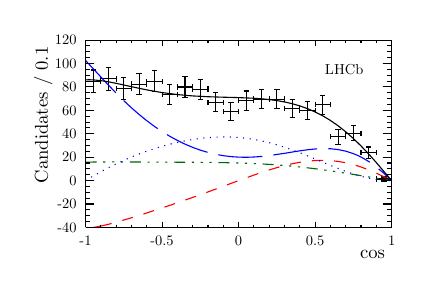
\begin{tikzpicture}
\pgfdeclareplotmark{cross} {
\pgfpathmoveto{\pgfpoint{-0.3\pgfplotmarksize}{\pgfplotmarksize}}
\pgfpathlineto{\pgfpoint{+0.3\pgfplotmarksize}{\pgfplotmarksize}}
\pgfpathlineto{\pgfpoint{+0.3\pgfplotmarksize}{0.3\pgfplotmarksize}}
\pgfpathlineto{\pgfpoint{+1\pgfplotmarksize}{0.3\pgfplotmarksize}}
\pgfpathlineto{\pgfpoint{+1\pgfplotmarksize}{-0.3\pgfplotmarksize}}
\pgfpathlineto{\pgfpoint{+0.3\pgfplotmarksize}{-0.3\pgfplotmarksize}}
\pgfpathlineto{\pgfpoint{+0.3\pgfplotmarksize}{-1.\pgfplotmarksize}}
\pgfpathlineto{\pgfpoint{-0.3\pgfplotmarksize}{-1.\pgfplotmarksize}}
\pgfpathlineto{\pgfpoint{-0.3\pgfplotmarksize}{-0.3\pgfplotmarksize}}
\pgfpathlineto{\pgfpoint{-1.\pgfplotmarksize}{-0.3\pgfplotmarksize}}
\pgfpathlineto{\pgfpoint{-1.\pgfplotmarksize}{0.3\pgfplotmarksize}}
\pgfpathlineto{\pgfpoint{-0.3\pgfplotmarksize}{0.3\pgfplotmarksize}}
\pgfpathclose
\pgfusepathqstroke
}
\pgfdeclareplotmark{cross*} {
\pgfpathmoveto{\pgfpoint{-0.3\pgfplotmarksize}{\pgfplotmarksize}}
\pgfpathlineto{\pgfpoint{+0.3\pgfplotmarksize}{\pgfplotmarksize}}
\pgfpathlineto{\pgfpoint{+0.3\pgfplotmarksize}{0.3\pgfplotmarksize}}
\pgfpathlineto{\pgfpoint{+1\pgfplotmarksize}{0.3\pgfplotmarksize}}
\pgfpathlineto{\pgfpoint{+1\pgfplotmarksize}{-0.3\pgfplotmarksize}}
\pgfpathlineto{\pgfpoint{+0.3\pgfplotmarksize}{-0.3\pgfplotmarksize}}
\pgfpathlineto{\pgfpoint{+0.3\pgfplotmarksize}{-1.\pgfplotmarksize}}
\pgfpathlineto{\pgfpoint{-0.3\pgfplotmarksize}{-1.\pgfplotmarksize}}
\pgfpathlineto{\pgfpoint{-0.3\pgfplotmarksize}{-0.3\pgfplotmarksize}}
\pgfpathlineto{\pgfpoint{-1.\pgfplotmarksize}{-0.3\pgfplotmarksize}}
\pgfpathlineto{\pgfpoint{-1.\pgfplotmarksize}{0.3\pgfplotmarksize}}
\pgfpathlineto{\pgfpoint{-0.3\pgfplotmarksize}{0.3\pgfplotmarksize}}
\pgfpathclose
\pgfusepathqfillstroke
}
\pgfdeclareplotmark{newstar} {
\pgfpathmoveto{\pgfqpoint{0pt}{\pgfplotmarksize}}
\pgfpathlineto{\pgfqpointpolar{44}{0.5\pgfplotmarksize}}
\pgfpathlineto{\pgfqpointpolar{18}{\pgfplotmarksize}}
\pgfpathlineto{\pgfqpointpolar{-20}{0.5\pgfplotmarksize}}
\pgfpathlineto{\pgfqpointpolar{-54}{\pgfplotmarksize}}
\pgfpathlineto{\pgfqpointpolar{-90}{0.5\pgfplotmarksize}}
\pgfpathlineto{\pgfqpointpolar{234}{\pgfplotmarksize}}
\pgfpathlineto{\pgfqpointpolar{198}{0.5\pgfplotmarksize}}
\pgfpathlineto{\pgfqpointpolar{162}{\pgfplotmarksize}}
\pgfpathlineto{\pgfqpointpolar{134}{0.5\pgfplotmarksize}}
\pgfpathclose
\pgfusepathqstroke
}
\pgfdeclareplotmark{newstar*} {
\pgfpathmoveto{\pgfqpoint{0pt}{\pgfplotmarksize}}
\pgfpathlineto{\pgfqpointpolar{44}{0.5\pgfplotmarksize}}
\pgfpathlineto{\pgfqpointpolar{18}{\pgfplotmarksize}}
\pgfpathlineto{\pgfqpointpolar{-20}{0.5\pgfplotmarksize}}
\pgfpathlineto{\pgfqpointpolar{-54}{\pgfplotmarksize}}
\pgfpathlineto{\pgfqpointpolar{-90}{0.5\pgfplotmarksize}}
\pgfpathlineto{\pgfqpointpolar{234}{\pgfplotmarksize}}
\pgfpathlineto{\pgfqpointpolar{198}{0.5\pgfplotmarksize}}
\pgfpathlineto{\pgfqpointpolar{162}{\pgfplotmarksize}}
\pgfpathlineto{\pgfqpointpolar{134}{0.5\pgfplotmarksize}}
\pgfpathclose
\pgfusepathqfillstroke
}
\definecolor{c}{rgb}{1,1,1};
\draw [color=c, fill=c] (0.1,3.20034) rectangle (4.9,6.21242);
\draw [color=c, fill=c] (0.772,3.68227) rectangle (4.66,6.06181);
\definecolor{c}{rgb}{0,0,0};
\draw [c] (0.772,3.68227) -- (0.772,6.06181) -- (4.66,6.06181) -- (4.66,3.68227) -- (0.772,3.68227);
\definecolor{c}{rgb}{1,1,1};
\draw [color=c, fill=c] (0.772,3.68227) rectangle (4.66,6.06181);
\definecolor{c}{rgb}{0,0,0};
\draw [c] (0.772,3.68227) -- (0.772,6.06181) -- (4.66,6.06181) -- (4.66,3.68227) -- (0.772,3.68227);
\draw [c,line width=0.4] (0.772,3.68227) -- (4.66,3.68227);
\draw [anchor= east] (4.66,3.34492) node[scale=0.672711, rotate=0]{$\cos\thetaK$};
\draw [c,line width=0.4] (0.772,3.75546) -- (0.772,3.68227);
\draw [c,line width=0.4] (0.9664,3.71887) -- (0.9664,3.68227);
\draw [c,line width=0.4] (1.1608,3.71887) -- (1.1608,3.68227);
\draw [c,line width=0.4] (1.3552,3.71887) -- (1.3552,3.68227);
\draw [c,line width=0.4] (1.5496,3.71887) -- (1.5496,3.68227);
\draw [c,line width=0.4] (1.744,3.75546) -- (1.744,3.68227);
\draw [c,line width=0.4] (1.9384,3.71887) -- (1.9384,3.68227);
\draw [c,line width=0.4] (2.1328,3.71887) -- (2.1328,3.68227);
\draw [c,line width=0.4] (2.3272,3.71887) -- (2.3272,3.68227);
\draw [c,line width=0.4] (2.5216,3.71887) -- (2.5216,3.68227);
\draw [c,line width=0.4] (2.716,3.75546) -- (2.716,3.68227);
\draw [c,line width=0.4] (2.9104,3.71887) -- (2.9104,3.68227);
\draw [c,line width=0.4] (3.1048,3.71887) -- (3.1048,3.68227);
\draw [c,line width=0.4] (3.2992,3.71887) -- (3.2992,3.68227);
\draw [c,line width=0.4] (3.4936,3.71887) -- (3.4936,3.68227);
\draw [c,line width=0.4] (3.688,3.75546) -- (3.688,3.68227);
\draw [c,line width=0.4] (3.8824,3.71887) -- (3.8824,3.68227);
\draw [c,line width=0.4] (4.0768,3.71887) -- (4.0768,3.68227);
\draw [c,line width=0.4] (4.2712,3.71887) -- (4.2712,3.68227);
\draw [c,line width=0.4] (4.4656,3.71887) -- (4.4656,3.68227);
\draw [c,line width=0.4] (4.66,3.75546) -- (4.66,3.68227);
\draw [anchor=base] (0.772,3.45937) node[scale=0.52322, rotate=0]{-1};
\draw [anchor=base] (1.744,3.45937) node[scale=0.52322, rotate=0]{-0.5};
\draw [anchor=base] (2.716,3.45937) node[scale=0.52322, rotate=0]{0};
\draw [anchor=base] (3.688,3.45937) node[scale=0.52322, rotate=0]{0.5};
\draw [anchor=base] (4.66,3.45937) node[scale=0.52322, rotate=0]{1};
\draw [c,line width=0.4] (0.772,6.06181) -- (4.66,6.06181);
\draw [c,line width=0.4] (0.772,5.98862) -- (0.772,6.06181);
\draw [c,line width=0.4] (0.9664,6.02522) -- (0.9664,6.06181);
\draw [c,line width=0.4] (1.1608,6.02522) -- (1.1608,6.06181);
\draw [c,line width=0.4] (1.3552,6.02522) -- (1.3552,6.06181);
\draw [c,line width=0.4] (1.5496,6.02522) -- (1.5496,6.06181);
\draw [c,line width=0.4] (1.744,5.98862) -- (1.744,6.06181);
\draw [c,line width=0.4] (1.9384,6.02522) -- (1.9384,6.06181);
\draw [c,line width=0.4] (2.1328,6.02522) -- (2.1328,6.06181);
\draw [c,line width=0.4] (2.3272,6.02522) -- (2.3272,6.06181);
\draw [c,line width=0.4] (2.5216,6.02522) -- (2.5216,6.06181);
\draw [c,line width=0.4] (2.716,5.98862) -- (2.716,6.06181);
\draw [c,line width=0.4] (2.9104,6.02522) -- (2.9104,6.06181);
\draw [c,line width=0.4] (3.1048,6.02522) -- (3.1048,6.06181);
\draw [c,line width=0.4] (3.2992,6.02522) -- (3.2992,6.06181);
\draw [c,line width=0.4] (3.4936,6.02522) -- (3.4936,6.06181);
\draw [c,line width=0.4] (3.688,5.98862) -- (3.688,6.06181);
\draw [c,line width=0.4] (3.8824,6.02522) -- (3.8824,6.06181);
\draw [c,line width=0.4] (4.0768,6.02522) -- (4.0768,6.06181);
\draw [c,line width=0.4] (4.2712,6.02522) -- (4.2712,6.06181);
\draw [c,line width=0.4] (4.4656,6.02522) -- (4.4656,6.06181);
\draw [c,line width=0.4] (4.66,5.98862) -- (4.66,6.06181);
\draw [c,line width=0.4] (0.772,3.68227) -- (0.772,6.06181);
\draw [anchor= east] (0.2344,6.06181) node[scale=0.672711, rotate=90]{Candidates / 0.1};
\draw [c,line width=0.4] (0.88576,3.68227) -- (0.772,3.68227);
\draw [c,line width=0.4] (0.82888,3.75663) -- (0.772,3.75663);
\draw [c,line width=0.4] (0.82888,3.83099) -- (0.772,3.83099);
\draw [c,line width=0.4] (0.82888,3.90535) -- (0.772,3.90535);
\draw [c,line width=0.4] (0.88576,3.97971) -- (0.772,3.97971);
\draw [c,line width=0.4] (0.82888,4.05407) -- (0.772,4.05407);
\draw [c,line width=0.4] (0.82888,4.12843) -- (0.772,4.12843);
\draw [c,line width=0.4] (0.82888,4.20279) -- (0.772,4.20279);
\draw [c,line width=0.4] (0.88576,4.27715) -- (0.772,4.27715);
\draw [c,line width=0.4] (0.82888,4.35152) -- (0.772,4.35152);
\draw [c,line width=0.4] (0.82888,4.42588) -- (0.772,4.42588);
\draw [c,line width=0.4] (0.82888,4.50024) -- (0.772,4.50024);
\draw [c,line width=0.4] (0.88576,4.5746) -- (0.772,4.5746);
\draw [c,line width=0.4] (0.82888,4.64896) -- (0.772,4.64896);
\draw [c,line width=0.4] (0.82888,4.72332) -- (0.772,4.72332);
\draw [c,line width=0.4] (0.82888,4.79768) -- (0.772,4.79768);
\draw [c,line width=0.4] (0.88576,4.87204) -- (0.772,4.87204);
\draw [c,line width=0.4] (0.82888,4.9464) -- (0.772,4.9464);
\draw [c,line width=0.4] (0.82888,5.02076) -- (0.772,5.02076);
\draw [c,line width=0.4] (0.82888,5.09512) -- (0.772,5.09512);
\draw [c,line width=0.4] (0.88576,5.16948) -- (0.772,5.16948);
\draw [c,line width=0.4] (0.82888,5.24384) -- (0.772,5.24384);
\draw [c,line width=0.4] (0.82888,5.3182) -- (0.772,5.3182);
\draw [c,line width=0.4] (0.82888,5.39257) -- (0.772,5.39257);
\draw [c,line width=0.4] (0.88576,5.46693) -- (0.772,5.46693);
\draw [c,line width=0.4] (0.82888,5.54129) -- (0.772,5.54129);
\draw [c,line width=0.4] (0.82888,5.61565) -- (0.772,5.61565);
\draw [c,line width=0.4] (0.82888,5.69001) -- (0.772,5.69001);
\draw [c,line width=0.4] (0.88576,5.76437) -- (0.772,5.76437);
\draw [c,line width=0.4] (0.82888,5.83873) -- (0.772,5.83873);
\draw [c,line width=0.4] (0.82888,5.91309) -- (0.772,5.91309);
\draw [c,line width=0.4] (0.82888,5.98745) -- (0.772,5.98745);
\draw [c,line width=0.4] (0.88576,6.06181) -- (0.772,6.06181);
\draw [anchor= east] (0.724,3.68227) node[scale=0.52322, rotate=0]{-40};
\draw [anchor= east] (0.724,3.97971) node[scale=0.52322, rotate=0]{-20};
\draw [anchor= east] (0.724,4.27715) node[scale=0.52322, rotate=0]{0};
\draw [anchor= east] (0.724,4.5746) node[scale=0.52322, rotate=0]{20};
\draw [anchor= east] (0.724,4.87204) node[scale=0.52322, rotate=0]{40};
\draw [anchor= east] (0.724,5.16948) node[scale=0.52322, rotate=0]{60};
\draw [anchor= east] (0.724,5.46693) node[scale=0.52322, rotate=0]{80};
\draw [anchor= east] (0.724,5.76437) node[scale=0.52322, rotate=0]{100};
\draw [anchor= east] (0.724,6.06181) node[scale=0.52322, rotate=0]{120};
\draw [c,line width=0.4] (4.66,3.68227) -- (4.66,6.06181);
\draw [c,line width=0.4] (4.54624,3.68227) -- (4.66,3.68227);
\draw [c,line width=0.4] (4.60312,3.75663) -- (4.66,3.75663);
\draw [c,line width=0.4] (4.60312,3.83099) -- (4.66,3.83099);
\draw [c,line width=0.4] (4.60312,3.90535) -- (4.66,3.90535);
\draw [c,line width=0.4] (4.54624,3.97971) -- (4.66,3.97971);
\draw [c,line width=0.4] (4.60312,4.05407) -- (4.66,4.05407);
\draw [c,line width=0.4] (4.60312,4.12843) -- (4.66,4.12843);
\draw [c,line width=0.4] (4.60312,4.20279) -- (4.66,4.20279);
\draw [c,line width=0.4] (4.54624,4.27715) -- (4.66,4.27715);
\draw [c,line width=0.4] (4.60312,4.35152) -- (4.66,4.35152);
\draw [c,line width=0.4] (4.60312,4.42588) -- (4.66,4.42588);
\draw [c,line width=0.4] (4.60312,4.50024) -- (4.66,4.50024);
\draw [c,line width=0.4] (4.54624,4.5746) -- (4.66,4.5746);
\draw [c,line width=0.4] (4.60312,4.64896) -- (4.66,4.64896);
\draw [c,line width=0.4] (4.60312,4.72332) -- (4.66,4.72332);
\draw [c,line width=0.4] (4.60312,4.79768) -- (4.66,4.79768);
\draw [c,line width=0.4] (4.54624,4.87204) -- (4.66,4.87204);
\draw [c,line width=0.4] (4.60312,4.9464) -- (4.66,4.9464);
\draw [c,line width=0.4] (4.60312,5.02076) -- (4.66,5.02076);
\draw [c,line width=0.4] (4.60312,5.09512) -- (4.66,5.09512);
\draw [c,line width=0.4] (4.54624,5.16948) -- (4.66,5.16948);
\draw [c,line width=0.4] (4.60312,5.24384) -- (4.66,5.24384);
\draw [c,line width=0.4] (4.60312,5.3182) -- (4.66,5.3182);
\draw [c,line width=0.4] (4.60312,5.39257) -- (4.66,5.39257);
\draw [c,line width=0.4] (4.54624,5.46693) -- (4.66,5.46693);
\draw [c,line width=0.4] (4.60312,5.54129) -- (4.66,5.54129);
\draw [c,line width=0.4] (4.60312,5.61565) -- (4.66,5.61565);
\draw [c,line width=0.4] (4.60312,5.69001) -- (4.66,5.69001);
\draw [c,line width=0.4] (4.54624,5.76437) -- (4.66,5.76437);
\draw [c,line width=0.4] (4.60312,5.83873) -- (4.66,5.83873);
\draw [c,line width=0.4] (4.60312,5.91309) -- (4.66,5.91309);
\draw [c,line width=0.4] (4.60312,5.98745) -- (4.66,5.98745);
\draw [c,line width=0.4] (4.54624,6.06181) -- (4.66,6.06181);
\draw [c] (0.8692,5.53998) -- (0.772,5.53998);
\draw [c] (0.772,5.50643) -- (0.772,5.57354);
\draw [c] (0.8692,5.53998) -- (0.9664,5.53998);
\draw [c] (0.9664,5.50643) -- (0.9664,5.57354);
\draw [c] (0.8692,5.53998) -- (0.8692,5.68166);
\draw [c] (0.835643,5.68166) -- (0.902757,5.68166);
\draw [c] (0.8692,5.53998) -- (0.8692,5.39831);
\draw [c] (0.835643,5.39831) -- (0.902757,5.39831);
\draw [c] (1.0636,5.56842) -- (0.9664,5.56842);
\draw [c] (0.9664,5.53486) -- (0.9664,5.60197);
\draw [c] (1.0636,5.56842) -- (1.1608,5.56842);
\draw [c] (1.1608,5.53486) -- (1.1608,5.60197);
\draw [c] (1.0636,5.56842) -- (1.0636,5.70972);
\draw [c] (1.03004,5.70972) -- (1.09716,5.70972);
\draw [c] (1.0636,5.56842) -- (1.0636,5.42711);
\draw [c] (1.03004,5.42711) -- (1.09716,5.42711);
\draw [c] (1.258,5.44696) -- (1.1608,5.44696);
\draw [c] (1.1608,5.4134) -- (1.1608,5.48052);
\draw [c] (1.258,5.44696) -- (1.3552,5.44696);
\draw [c] (1.3552,5.4134) -- (1.3552,5.48052);
\draw [c] (1.258,5.44696) -- (1.258,5.58349);
\draw [c] (1.22444,5.58349) -- (1.29156,5.58349);
\draw [c] (1.258,5.44696) -- (1.258,5.31043);
\draw [c] (1.22444,5.31043) -- (1.29156,5.31043);
\draw [c] (1.4524,5.50273) -- (1.3552,5.50273);
\draw [c] (1.3552,5.46918) -- (1.3552,5.53629);
\draw [c] (1.4524,5.50273) -- (1.5496,5.50273);
\draw [c] (1.5496,5.46918) -- (1.5496,5.53629);
\draw [c] (1.4524,5.50273) -- (1.4524,5.63754);
\draw [c] (1.41884,5.63754) -- (1.48596,5.63754);
\draw [c] (1.4524,5.50273) -- (1.4524,5.36793);
\draw [c] (1.41884,5.36793) -- (1.48596,5.36793);
\draw [c] (1.6468,5.53811) -- (1.5496,5.53811);
\draw [c] (1.5496,5.50455) -- (1.5496,5.57166);
\draw [c] (1.6468,5.53811) -- (1.744,5.53811);
\draw [c] (1.744,5.50455) -- (1.744,5.57166);
\draw [c] (1.6468,5.53811) -- (1.6468,5.67306);
\draw [c] (1.61324,5.67306) -- (1.68036,5.67306);
\draw [c] (1.6468,5.53811) -- (1.6468,5.40315);
\draw [c] (1.61324,5.40315) -- (1.68036,5.40315);
\draw [c] (1.8412,5.3681) -- (1.744,5.3681);
\draw [c] (1.744,5.33454) -- (1.744,5.40165);
\draw [c] (1.8412,5.3681) -- (1.9384,5.3681);
\draw [c] (1.9384,5.33454) -- (1.9384,5.40165);
\draw [c] (1.8412,5.3681) -- (1.8412,5.49512);
\draw [c] (1.80764,5.49512) -- (1.87476,5.49512);
\draw [c] (1.8412,5.3681) -- (1.8412,5.24107);
\draw [c] (1.80764,5.24107) -- (1.87476,5.24107);
\draw [c] (2.0356,5.4665) -- (1.9384,5.4665);
\draw [c] (1.9384,5.43295) -- (1.9384,5.50006);
\draw [c] (2.0356,5.4665) -- (2.1328,5.4665);
\draw [c] (2.1328,5.43295) -- (2.1328,5.50006);
\draw [c] (2.0356,5.4665) -- (2.0356,5.59827);
\draw [c] (2.00204,5.59827) -- (2.06916,5.59827);
\draw [c] (2.0356,5.4665) -- (2.0356,5.33473);
\draw [c] (2.00204,5.33473) -- (2.06916,5.33473);
\draw [c] (2.23,5.43953) -- (2.1328,5.43953);
\draw [c] (2.1328,5.40597) -- (2.1328,5.47309);
\draw [c] (2.23,5.43953) -- (2.3272,5.43953);
\draw [c] (2.3272,5.40597) -- (2.3272,5.47309);
\draw [c] (2.23,5.43953) -- (2.23,5.56678);
\draw [c] (2.19644,5.56678) -- (2.26356,5.56678);
\draw [c] (2.23,5.43953) -- (2.23,5.31228);
\draw [c] (2.19644,5.31228) -- (2.26356,5.31228);
\draw [c] (2.4244,5.2713) -- (2.3272,5.2713);
\draw [c] (2.3272,5.23774) -- (2.3272,5.30485);
\draw [c] (2.4244,5.2713) -- (2.5216,5.2713);
\draw [c] (2.5216,5.23774) -- (2.5216,5.30485);
\draw [c] (2.4244,5.2713) -- (2.4244,5.39227);
\draw [c] (2.39084,5.39227) -- (2.45796,5.39227);
\draw [c] (2.4244,5.2713) -- (2.4244,5.15033);
\draw [c] (2.39084,5.15033) -- (2.45796,5.15033);
\draw [c] (2.6188,5.15486) -- (2.5216,5.15486);
\draw [c] (2.5216,5.1213) -- (2.5216,5.18842);
\draw [c] (2.6188,5.15486) -- (2.716,5.15486);
\draw [c] (2.716,5.1213) -- (2.716,5.18842);
\draw [c] (2.6188,5.15486) -- (2.6188,5.26834);
\draw [c] (2.58524,5.26834) -- (2.65236,5.26834);
\draw [c] (2.6188,5.15486) -- (2.6188,5.04137);
\draw [c] (2.58524,5.04137) -- (2.65236,5.04137);
\draw [c] (2.8132,5.29357) -- (2.716,5.29357);
\draw [c] (2.716,5.26001) -- (2.716,5.32713);
\draw [c] (2.8132,5.29357) -- (2.9104,5.29357);
\draw [c] (2.9104,5.26001) -- (2.9104,5.32713);
\draw [c] (2.8132,5.29357) -- (2.8132,5.41525);
\draw [c] (2.77964,5.41525) -- (2.84676,5.41525);
\draw [c] (2.8132,5.29357) -- (2.8132,5.17189);
\draw [c] (2.77964,5.17189) -- (2.84676,5.17189);
\draw [c] (3.0076,5.31225) -- (2.9104,5.31225);
\draw [c] (2.9104,5.2787) -- (2.9104,5.34581);
\draw [c] (3.0076,5.31225) -- (3.1048,5.31225);
\draw [c] (3.1048,5.2787) -- (3.1048,5.34581);
\draw [c] (3.0076,5.31225) -- (3.0076,5.43309);
\draw [c] (2.97404,5.43309) -- (3.04116,5.43309);
\draw [c] (3.0076,5.31225) -- (3.0076,5.19142);
\draw [c] (2.97404,5.19142) -- (3.04116,5.19142);
\draw [c] (3.202,5.31224) -- (3.1048,5.31224);
\draw [c] (3.1048,5.27868) -- (3.1048,5.3458);
\draw [c] (3.202,5.31224) -- (3.2992,5.31224);
\draw [c] (3.2992,5.27868) -- (3.2992,5.3458);
\draw [c] (3.202,5.31224) -- (3.202,5.43256);
\draw [c] (3.16844,5.43256) -- (3.23556,5.43256);
\draw [c] (3.202,5.31224) -- (3.202,5.19192);
\draw [c] (3.16844,5.19192) -- (3.23556,5.19192);
\draw [c] (3.3964,5.19601) -- (3.2992,5.19601);
\draw [c] (3.2992,5.16245) -- (3.2992,5.22957);
\draw [c] (3.3964,5.19601) -- (3.4936,5.19601);
\draw [c] (3.4936,5.16245) -- (3.4936,5.22957);
\draw [c] (3.3964,5.19601) -- (3.3964,5.31245);
\draw [c] (3.36284,5.31245) -- (3.42996,5.31245);
\draw [c] (3.3964,5.19601) -- (3.3964,5.07958);
\draw [c] (3.36284,5.07958) -- (3.42996,5.07958);
\draw [c] (3.5908,5.16841) -- (3.4936,5.16841);
\draw [c] (3.4936,5.13485) -- (3.4936,5.20197);
\draw [c] (3.5908,5.16841) -- (3.688,5.16841);
\draw [c] (3.688,5.13485) -- (3.688,5.20197);
\draw [c] (3.5908,5.16841) -- (3.5908,5.28525);
\draw [c] (3.55724,5.28525) -- (3.62436,5.28525);
\draw [c] (3.5908,5.16841) -- (3.5908,5.05158);
\draw [c] (3.55724,5.05158) -- (3.62436,5.05158);
\draw [c] (3.7852,5.24155) -- (3.688,5.24155);
\draw [c] (3.688,5.208) -- (3.688,5.27511);
\draw [c] (3.7852,5.24155) -- (3.8824,5.24155);
\draw [c] (3.8824,5.208) -- (3.8824,5.27511);
\draw [c] (3.7852,5.24155) -- (3.7852,5.36086);
\draw [c] (3.75164,5.36086) -- (3.81876,5.36086);
\draw [c] (3.7852,5.24155) -- (3.7852,5.12225);
\draw [c] (3.75164,5.12225) -- (3.81876,5.12225);
\draw [c] (3.9796,4.83424) -- (3.8824,4.83424);
\draw [c] (3.8824,4.80068) -- (3.8824,4.86779);
\draw [c] (3.9796,4.83424) -- (4.0768,4.83424);
\draw [c] (4.0768,4.80068) -- (4.0768,4.86779);
\draw [c] (3.9796,4.83424) -- (3.9796,4.92924);
\draw [c] (3.94604,4.92924) -- (4.01316,4.92924);
\draw [c] (3.9796,4.83424) -- (3.9796,4.73924);
\draw [c] (3.94604,4.73924) -- (4.01316,4.73924);
\draw [c] (4.174,4.87912) -- (4.0768,4.87912);
\draw [c] (4.0768,4.84557) -- (4.0768,4.91268);
\draw [c] (4.174,4.87912) -- (4.2712,4.87912);
\draw [c] (4.2712,4.84557) -- (4.2712,4.91268);
\draw [c] (4.174,4.87912) -- (4.174,4.97502);
\draw [c] (4.14044,4.97502) -- (4.20756,4.97502);
\draw [c] (4.174,4.87912) -- (4.174,4.78323);
\draw [c] (4.14044,4.78323) -- (4.20756,4.78323);
\draw [c] (4.3684,4.63391) -- (4.2712,4.63391);
\draw [c] (4.2712,4.60035) -- (4.2712,4.66747);
\draw [c] (4.3684,4.63391) -- (4.4656,4.63391);
\draw [c] (4.4656,4.60035) -- (4.4656,4.66747);
\draw [c] (4.3684,4.63391) -- (4.3684,4.70429);
\draw [c] (4.33484,4.70429) -- (4.40196,4.70429);
\draw [c] (4.3684,4.63391) -- (4.3684,4.56353);
\draw [c] (4.33484,4.56353) -- (4.40196,4.56353);
\draw [c] (4.5628,4.29753) -- (4.4656,4.29753);
\draw [c] (4.4656,4.26397) -- (4.4656,4.33109);
\draw [c] (4.5628,4.29753) -- (4.66,4.29753);
\draw [c] (4.66,4.26397) -- (4.66,4.33109);
\draw [c] (4.5628,4.29753) -- (4.5628,4.32295);
\draw [c] (4.52924,4.32295) -- (4.59636,4.32295);
\draw [c] (4.5628,4.29753) -- (4.5628,4.27211);
\draw [c] (4.52924,4.27211) -- (4.59636,4.27211);
\foreach \P in
 {(0.8692,5.53998),(1.0636,5.56842),(1.258,5.44696),(1.4524,5.50273),(1.6468,5.53811),(1.8412,5.3681),(2.0356,5.4665),(2.23,5.43953),(2.4244,5.2713),(2.6188,5.15486),(2.8132,5.29357),(3.0076,5.31225),(3.202,5.31224),(3.3964,5.19601),(3.5908,5.16841),
(3.7852,5.24155),(3.9796,4.83424),(4.174,4.87912),(4.3684,4.63391),(4.5628,4.29753)}{\draw[mark options={color=c,fill=c},mark size=1.201201pt,mark=] plot coordinates {\P};}
\definecolor{c}{rgb}{1,0,0};
\draw [c,dash pattern=on 4pt off 4pt] (0.873342,3.68227) -- (0.9664,3.69993);
\draw [c,dash pattern=on 4pt off 4pt] (0.9664,3.69993) -- (1.0636,3.7225) -- (1.1608,3.74806) -- (1.3552,3.80497) -- (1.5496,3.86625) -- (1.744,3.92998) -- (1.9384,3.99564) -- (2.1328,4.06338) -- (2.3272,4.1333) -- (2.5216,4.20499) -- (2.716,4.27715)
 -- (2.9104,4.34749) -- (3.0076,4.38096) -- (3.1048,4.41264) -- (3.202,4.44198) -- (3.2992,4.46838) -- (3.3964,4.49122) -- (3.4936,4.50989) -- (3.5908,4.52378) -- (3.688,4.53231) -- (3.7852,4.53498) -- (3.8824,4.53134) -- (3.9796,4.52108) --
 (4.0768,4.50403) -- (4.174,4.4802) -- (4.2712,4.44982) -- (4.3684,4.41337) -- (4.4656,4.37163) -- (4.5628,4.32572) -- (4.66,4.27715) -- (4.66,4.27715) -- (4.66,4.27715);
\definecolor{c}{rgb}{0,0.4,0};
\draw [c,dash pattern=on 4pt off 2.4pt on 0.8pt off 2.4pt on 0.8pt off 2.4pt on 0.8pt off 2.4pt] (0.772,4.511) -- (0.772,4.511);
\draw [c,dash pattern=on 4pt off 2.4pt on 0.8pt off 2.4pt on 0.8pt off 2.4pt on 0.8pt off 2.4pt] (0.772,4.511) -- (0.8692,4.51284) -- (0.9664,4.51387) -- (1.1608,4.51432) -- (1.3552,4.51364) -- (1.5496,4.51264) -- (1.744,4.5117) -- (1.9384,4.51088)
 -- (2.1328,4.50991) -- (2.3272,4.50835) -- (2.5216,4.50557) -- (2.6188,4.50351) -- (2.716,4.50089) -- (2.8132,4.49762) -- (2.9104,4.49361) -- (3.0076,4.48879) -- (3.1048,4.48308) -- (3.202,4.47643) -- (3.2992,4.46878) -- (3.3964,4.46011) --
 (3.4936,4.45039) -- (3.5908,4.43962) -- (3.688,4.42783) -- (3.7852,4.41506) -- (3.8824,4.40138) -- (3.9796,4.38688) -- (4.0768,4.37168) -- (4.2712,4.33987) -- (4.4656,4.30761) -- (4.5628,4.29199) -- (4.66,4.27715) -- (4.66,4.27715) --
 (4.66,4.27715);
\definecolor{c}{rgb}{0,0,1};
\draw [c,dotted] (0.772,4.27715) -- (0.772,4.27715);
\draw [c,dotted] (0.772,4.27715) -- (0.8692,4.33452) -- (0.9664,4.38926) -- (1.0636,4.44099) -- (1.1608,4.4895) -- (1.258,4.53471) -- (1.3552,4.57663) -- (1.4524,4.6153) -- (1.5496,4.65081) -- (1.6468,4.68322) -- (1.744,4.71258) -- (1.8412,4.73891)
 -- (1.9384,4.76217) -- (2.0356,4.78232) -- (2.1328,4.79925) -- (2.23,4.81282) -- (2.3272,4.82288) -- (2.4244,4.82925) -- (2.5216,4.83174) -- (2.6188,4.8302) -- (2.716,4.82448) -- (2.8132,4.81447) -- (2.9104,4.80014) -- (3.0076,4.78149) --
 (3.1048,4.75863) -- (3.202,4.73176) -- (3.2992,4.70118) -- (3.3964,4.66728) -- (3.4936,4.63061) -- (3.5908,4.59178) -- (3.688,4.55154) -- (3.8824,4.47027) -- (3.9796,4.43117) -- (4.0768,4.39444) -- (4.174,4.36113) -- (4.2226,4.34607) --
 (4.2712,4.33225) -- (4.3198,4.31976) -- (4.3684,4.30872) -- (4.417,4.29922) -- (4.4656,4.29134) -- (4.5142,4.28516) -- (4.5628,4.28071) -- (4.6114,4.27804) -- (4.66,4.27715) -- (4.66,4.27715) -- (4.66,4.27715);
\draw [c,dash pattern=on 16pt off 4pt] (0.772,5.80367) -- (0.772,5.80367);
\draw [c,dash pattern=on 16pt off 4pt] (0.772,5.80367) -- (0.9664,5.59361) -- (1.0636,5.48951) -- (1.1608,5.38871) -- (1.258,5.29251) -- (1.3552,5.20174) -- (1.4524,5.11692) -- (1.5496,5.03835) -- (1.6468,4.96614) -- (1.744,4.9003) --
 (1.8412,4.84078) -- (1.9384,4.78749) -- (2.0356,4.74036) -- (2.1328,4.69928) -- (2.23,4.66418) -- (2.3272,4.63499) -- (2.4244,4.61162) -- (2.5216,4.59396) -- (2.6188,4.58188) -- (2.716,4.57517) -- (2.8132,4.57355) -- (2.9104,4.57664) --
 (3.0076,4.58393) -- (3.1048,4.59478) -- (3.2992,4.6238) -- (3.4936,4.65542) -- (3.5908,4.66894) -- (3.688,4.67892) -- (3.7852,4.68376) -- (3.8824,4.6818) -- (3.9796,4.67143) -- (4.0768,4.65115) -- (4.174,4.61963) -- (4.2226,4.59933) --
 (4.2712,4.57587) -- (4.3198,4.54921) -- (4.3684,4.51932) -- (4.417,4.48623) -- (4.4656,4.45001) -- (4.5628,4.3687) -- (4.66,4.27715) -- (4.66,4.27715) -- (4.66,4.27715);
\definecolor{c}{rgb}{0,0,0};
\draw [c] (0.772,5.55672) -- (0.772,5.55672);
\draw [c] (0.772,5.55672) -- (0.8206,5.55778) -- (0.8692,5.55621) -- (0.9664,5.54686) -- (1.0636,5.53152) -- (1.1608,5.51249) -- (1.3552,5.47008) -- (1.5496,5.42932) -- (1.744,5.39523) -- (1.9384,5.36972) -- (2.1328,5.35261) -- (2.3272,5.34235) --
 (2.5216,5.33639) -- (2.716,5.33133) -- (2.9104,5.32302) -- (3.0076,5.31614) -- (3.1048,5.30653) -- (3.202,5.29347) -- (3.2992,5.27621) -- (3.3964,5.25395) -- (3.4936,5.22591) -- (3.5908,5.19131) -- (3.688,5.14939) -- (3.7852,5.0995) --
 (3.8824,5.04106) -- (3.9796,4.97365) -- (4.0768,4.89707) -- (4.174,4.81137) -- (4.2712,4.71696) -- (4.3684,4.61466) -- (4.4656,4.50583) -- (4.66,4.27715) -- (4.66,4.27715) -- (4.66,4.27715);
\draw [c,line width=0.4] (0.772,3.68227) -- (4.66,3.68227);
\draw [c,line width=0.4] (0.772,3.75546) -- (0.772,3.68227);
\draw [c,line width=0.4] (0.9664,3.71887) -- (0.9664,3.68227);
\draw [c,line width=0.4] (1.1608,3.71887) -- (1.1608,3.68227);
\draw [c,line width=0.4] (1.3552,3.71887) -- (1.3552,3.68227);
\draw [c,line width=0.4] (1.5496,3.71887) -- (1.5496,3.68227);
\draw [c,line width=0.4] (1.744,3.75546) -- (1.744,3.68227);
\draw [c,line width=0.4] (1.9384,3.71887) -- (1.9384,3.68227);
\draw [c,line width=0.4] (2.1328,3.71887) -- (2.1328,3.68227);
\draw [c,line width=0.4] (2.3272,3.71887) -- (2.3272,3.68227);
\draw [c,line width=0.4] (2.5216,3.71887) -- (2.5216,3.68227);
\draw [c,line width=0.4] (2.716,3.75546) -- (2.716,3.68227);
\draw [c,line width=0.4] (2.9104,3.71887) -- (2.9104,3.68227);
\draw [c,line width=0.4] (3.1048,3.71887) -- (3.1048,3.68227);
\draw [c,line width=0.4] (3.2992,3.71887) -- (3.2992,3.68227);
\draw [c,line width=0.4] (3.4936,3.71887) -- (3.4936,3.68227);
\draw [c,line width=0.4] (3.688,3.75546) -- (3.688,3.68227);
\draw [c,line width=0.4] (3.8824,3.71887) -- (3.8824,3.68227);
\draw [c,line width=0.4] (4.0768,3.71887) -- (4.0768,3.68227);
\draw [c,line width=0.4] (4.2712,3.71887) -- (4.2712,3.68227);
\draw [c,line width=0.4] (4.4656,3.71887) -- (4.4656,3.68227);
\draw [c,line width=0.4] (4.66,3.75546) -- (4.66,3.68227);
\draw [c,line width=0.4] (0.772,6.06181) -- (4.66,6.06181);
\draw [c,line width=0.4] (0.772,5.98862) -- (0.772,6.06181);
\draw [c,line width=0.4] (0.9664,6.02522) -- (0.9664,6.06181);
\draw [c,line width=0.4] (1.1608,6.02522) -- (1.1608,6.06181);
\draw [c,line width=0.4] (1.3552,6.02522) -- (1.3552,6.06181);
\draw [c,line width=0.4] (1.5496,6.02522) -- (1.5496,6.06181);
\draw [c,line width=0.4] (1.744,5.98862) -- (1.744,6.06181);
\draw [c,line width=0.4] (1.9384,6.02522) -- (1.9384,6.06181);
\draw [c,line width=0.4] (2.1328,6.02522) -- (2.1328,6.06181);
\draw [c,line width=0.4] (2.3272,6.02522) -- (2.3272,6.06181);
\draw [c,line width=0.4] (2.5216,6.02522) -- (2.5216,6.06181);
\draw [c,line width=0.4] (2.716,5.98862) -- (2.716,6.06181);
\draw [c,line width=0.4] (2.9104,6.02522) -- (2.9104,6.06181);
\draw [c,line width=0.4] (3.1048,6.02522) -- (3.1048,6.06181);
\draw [c,line width=0.4] (3.2992,6.02522) -- (3.2992,6.06181);
\draw [c,line width=0.4] (3.4936,6.02522) -- (3.4936,6.06181);
\draw [c,line width=0.4] (3.688,5.98862) -- (3.688,6.06181);
\draw [c,line width=0.4] (3.8824,6.02522) -- (3.8824,6.06181);
\draw [c,line width=0.4] (4.0768,6.02522) -- (4.0768,6.06181);
\draw [c,line width=0.4] (4.2712,6.02522) -- (4.2712,6.06181);
\draw [c,line width=0.4] (4.4656,6.02522) -- (4.4656,6.06181);
\draw [c,line width=0.4] (4.66,5.98862) -- (4.66,6.06181);
\draw [c,line width=0.4] (0.772,3.68227) -- (0.772,6.06181);
\draw [c,line width=0.4] (0.88576,3.68227) -- (0.772,3.68227);
\draw [c,line width=0.4] (0.82888,3.75663) -- (0.772,3.75663);
\draw [c,line width=0.4] (0.82888,3.83099) -- (0.772,3.83099);
\draw [c,line width=0.4] (0.82888,3.90535) -- (0.772,3.90535);
\draw [c,line width=0.4] (0.88576,3.97971) -- (0.772,3.97971);
\draw [c,line width=0.4] (0.82888,4.05407) -- (0.772,4.05407);
\draw [c,line width=0.4] (0.82888,4.12843) -- (0.772,4.12843);
\draw [c,line width=0.4] (0.82888,4.20279) -- (0.772,4.20279);
\draw [c,line width=0.4] (0.88576,4.27715) -- (0.772,4.27715);
\draw [c,line width=0.4] (0.82888,4.35152) -- (0.772,4.35152);
\draw [c,line width=0.4] (0.82888,4.42588) -- (0.772,4.42588);
\draw [c,line width=0.4] (0.82888,4.50024) -- (0.772,4.50024);
\draw [c,line width=0.4] (0.88576,4.5746) -- (0.772,4.5746);
\draw [c,line width=0.4] (0.82888,4.64896) -- (0.772,4.64896);
\draw [c,line width=0.4] (0.82888,4.72332) -- (0.772,4.72332);
\draw [c,line width=0.4] (0.82888,4.79768) -- (0.772,4.79768);
\draw [c,line width=0.4] (0.88576,4.87204) -- (0.772,4.87204);
\draw [c,line width=0.4] (0.82888,4.9464) -- (0.772,4.9464);
\draw [c,line width=0.4] (0.82888,5.02076) -- (0.772,5.02076);
\draw [c,line width=0.4] (0.82888,5.09512) -- (0.772,5.09512);
\draw [c,line width=0.4] (0.88576,5.16948) -- (0.772,5.16948);
\draw [c,line width=0.4] (0.82888,5.24384) -- (0.772,5.24384);
\draw [c,line width=0.4] (0.82888,5.3182) -- (0.772,5.3182);
\draw [c,line width=0.4] (0.82888,5.39257) -- (0.772,5.39257);
\draw [c,line width=0.4] (0.88576,5.46693) -- (0.772,5.46693);
\draw [c,line width=0.4] (0.82888,5.54129) -- (0.772,5.54129);
\draw [c,line width=0.4] (0.82888,5.61565) -- (0.772,5.61565);
\draw [c,line width=0.4] (0.82888,5.69001) -- (0.772,5.69001);
\draw [c,line width=0.4] (0.88576,5.76437) -- (0.772,5.76437);
\draw [c,line width=0.4] (0.82888,5.83873) -- (0.772,5.83873);
\draw [c,line width=0.4] (0.82888,5.91309) -- (0.772,5.91309);
\draw [c,line width=0.4] (0.82888,5.98745) -- (0.772,5.98745);
\draw [c,line width=0.4] (0.88576,6.06181) -- (0.772,6.06181);
\draw [c,line width=0.4] (4.66,3.68227) -- (4.66,6.06181);
\draw [c,line width=0.4] (4.54624,3.68227) -- (4.66,3.68227);
\draw [c,line width=0.4] (4.60312,3.75663) -- (4.66,3.75663);
\draw [c,line width=0.4] (4.60312,3.83099) -- (4.66,3.83099);
\draw [c,line width=0.4] (4.60312,3.90535) -- (4.66,3.90535);
\draw [c,line width=0.4] (4.54624,3.97971) -- (4.66,3.97971);
\draw [c,line width=0.4] (4.60312,4.05407) -- (4.66,4.05407);
\draw [c,line width=0.4] (4.60312,4.12843) -- (4.66,4.12843);
\draw [c,line width=0.4] (4.60312,4.20279) -- (4.66,4.20279);
\draw [c,line width=0.4] (4.54624,4.27715) -- (4.66,4.27715);
\draw [c,line width=0.4] (4.60312,4.35152) -- (4.66,4.35152);
\draw [c,line width=0.4] (4.60312,4.42588) -- (4.66,4.42588);
\draw [c,line width=0.4] (4.60312,4.50024) -- (4.66,4.50024);
\draw [c,line width=0.4] (4.54624,4.5746) -- (4.66,4.5746);
\draw [c,line width=0.4] (4.60312,4.64896) -- (4.66,4.64896);
\draw [c,line width=0.4] (4.60312,4.72332) -- (4.66,4.72332);
\draw [c,line width=0.4] (4.60312,4.79768) -- (4.66,4.79768);
\draw [c,line width=0.4] (4.54624,4.87204) -- (4.66,4.87204);
\draw [c,line width=0.4] (4.60312,4.9464) -- (4.66,4.9464);
\draw [c,line width=0.4] (4.60312,5.02076) -- (4.66,5.02076);
\draw [c,line width=0.4] (4.60312,5.09512) -- (4.66,5.09512);
\draw [c,line width=0.4] (4.54624,5.16948) -- (4.66,5.16948);
\draw [c,line width=0.4] (4.60312,5.24384) -- (4.66,5.24384);
\draw [c,line width=0.4] (4.60312,5.3182) -- (4.66,5.3182);
\draw [c,line width=0.4] (4.60312,5.39257) -- (4.66,5.39257);
\draw [c,line width=0.4] (4.54624,5.46693) -- (4.66,5.46693);
\draw [c,line width=0.4] (4.60312,5.54129) -- (4.66,5.54129);
\draw [c,line width=0.4] (4.60312,5.61565) -- (4.66,5.61565);
\draw [c,line width=0.4] (4.60312,5.69001) -- (4.66,5.69001);
\draw [c,line width=0.4] (4.54624,5.76437) -- (4.66,5.76437);
\draw [c,line width=0.4] (4.60312,5.83873) -- (4.66,5.83873);
\draw [c,line width=0.4] (4.60312,5.91309) -- (4.66,5.91309);
\draw [c,line width=0.4] (4.60312,5.98745) -- (4.66,5.98745);
\draw [c,line width=0.4] (4.54624,6.06181) -- (4.66,6.06181);
\draw [anchor= west] (3.748,5.6853) node[scale=0.52322, rotate=0]{LHCb};
\end{tikzpicture}
}
    \caption{}
    \label{angPlot_ctk}
  \end{subfigure}%
  \hfill%
  \begin{subfigure}{0.5\textwidth}
    \tikzsetnextfilename{angPlot_helcosthetaL}
    \scalebox{1.3}{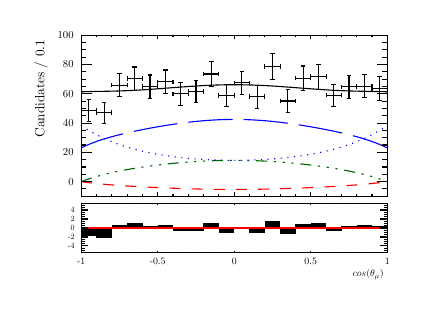
\begin{tikzpicture}
\pgfdeclareplotmark{cross} {
\pgfpathmoveto{\pgfpoint{-0.3\pgfplotmarksize}{\pgfplotmarksize}}
\pgfpathlineto{\pgfpoint{+0.3\pgfplotmarksize}{\pgfplotmarksize}}
\pgfpathlineto{\pgfpoint{+0.3\pgfplotmarksize}{0.3\pgfplotmarksize}}
\pgfpathlineto{\pgfpoint{+1\pgfplotmarksize}{0.3\pgfplotmarksize}}
\pgfpathlineto{\pgfpoint{+1\pgfplotmarksize}{-0.3\pgfplotmarksize}}
\pgfpathlineto{\pgfpoint{+0.3\pgfplotmarksize}{-0.3\pgfplotmarksize}}
\pgfpathlineto{\pgfpoint{+0.3\pgfplotmarksize}{-1.\pgfplotmarksize}}
\pgfpathlineto{\pgfpoint{-0.3\pgfplotmarksize}{-1.\pgfplotmarksize}}
\pgfpathlineto{\pgfpoint{-0.3\pgfplotmarksize}{-0.3\pgfplotmarksize}}
\pgfpathlineto{\pgfpoint{-1.\pgfplotmarksize}{-0.3\pgfplotmarksize}}
\pgfpathlineto{\pgfpoint{-1.\pgfplotmarksize}{0.3\pgfplotmarksize}}
\pgfpathlineto{\pgfpoint{-0.3\pgfplotmarksize}{0.3\pgfplotmarksize}}
\pgfpathclose
\pgfusepathqstroke
}
\pgfdeclareplotmark{cross*} {
\pgfpathmoveto{\pgfpoint{-0.3\pgfplotmarksize}{\pgfplotmarksize}}
\pgfpathlineto{\pgfpoint{+0.3\pgfplotmarksize}{\pgfplotmarksize}}
\pgfpathlineto{\pgfpoint{+0.3\pgfplotmarksize}{0.3\pgfplotmarksize}}
\pgfpathlineto{\pgfpoint{+1\pgfplotmarksize}{0.3\pgfplotmarksize}}
\pgfpathlineto{\pgfpoint{+1\pgfplotmarksize}{-0.3\pgfplotmarksize}}
\pgfpathlineto{\pgfpoint{+0.3\pgfplotmarksize}{-0.3\pgfplotmarksize}}
\pgfpathlineto{\pgfpoint{+0.3\pgfplotmarksize}{-1.\pgfplotmarksize}}
\pgfpathlineto{\pgfpoint{-0.3\pgfplotmarksize}{-1.\pgfplotmarksize}}
\pgfpathlineto{\pgfpoint{-0.3\pgfplotmarksize}{-0.3\pgfplotmarksize}}
\pgfpathlineto{\pgfpoint{-1.\pgfplotmarksize}{-0.3\pgfplotmarksize}}
\pgfpathlineto{\pgfpoint{-1.\pgfplotmarksize}{0.3\pgfplotmarksize}}
\pgfpathlineto{\pgfpoint{-0.3\pgfplotmarksize}{0.3\pgfplotmarksize}}
\pgfpathclose
\pgfusepathqfillstroke
}
\pgfdeclareplotmark{newstar} {
\pgfpathmoveto{\pgfqpoint{0pt}{\pgfplotmarksize}}
\pgfpathlineto{\pgfqpointpolar{44}{0.5\pgfplotmarksize}}
\pgfpathlineto{\pgfqpointpolar{18}{\pgfplotmarksize}}
\pgfpathlineto{\pgfqpointpolar{-20}{0.5\pgfplotmarksize}}
\pgfpathlineto{\pgfqpointpolar{-54}{\pgfplotmarksize}}
\pgfpathlineto{\pgfqpointpolar{-90}{0.5\pgfplotmarksize}}
\pgfpathlineto{\pgfqpointpolar{234}{\pgfplotmarksize}}
\pgfpathlineto{\pgfqpointpolar{198}{0.5\pgfplotmarksize}}
\pgfpathlineto{\pgfqpointpolar{162}{\pgfplotmarksize}}
\pgfpathlineto{\pgfqpointpolar{134}{0.5\pgfplotmarksize}}
\pgfpathclose
\pgfusepathqstroke
}
\pgfdeclareplotmark{newstar*} {
\pgfpathmoveto{\pgfqpoint{0pt}{\pgfplotmarksize}}
\pgfpathlineto{\pgfqpointpolar{44}{0.5\pgfplotmarksize}}
\pgfpathlineto{\pgfqpointpolar{18}{\pgfplotmarksize}}
\pgfpathlineto{\pgfqpointpolar{-20}{0.5\pgfplotmarksize}}
\pgfpathlineto{\pgfqpointpolar{-54}{\pgfplotmarksize}}
\pgfpathlineto{\pgfqpointpolar{-90}{0.5\pgfplotmarksize}}
\pgfpathlineto{\pgfqpointpolar{234}{\pgfplotmarksize}}
\pgfpathlineto{\pgfqpointpolar{198}{0.5\pgfplotmarksize}}
\pgfpathlineto{\pgfqpointpolar{162}{\pgfplotmarksize}}
\pgfpathlineto{\pgfqpointpolar{134}{0.5\pgfplotmarksize}}
\pgfpathclose
\pgfusepathqfillstroke
}
\definecolor{c}{rgb}{1,1,1};
\draw [color=c, fill=c] (5.1,3.47328) rectangle (9.9,6.74224);
\draw [color=c, fill=c] (5.1,4.51934) rectangle (9.9,6.74224);
\draw [color=c, fill=c] (5.772,4.60826) rectangle (9.66,6.65333);
\definecolor{c}{rgb}{0,0,0};
\draw [c] (5.772,4.60826) -- (5.772,6.65333) -- (9.66,6.65333) -- (9.66,4.60826) -- (5.772,4.60826);
\definecolor{c}{rgb}{1,1,1};
\draw [color=c, fill=c] (5.772,4.60826) rectangle (9.66,6.65333);
\definecolor{c}{rgb}{0,0,0};
\draw [c] (5.772,4.60826) -- (5.772,6.65333) -- (9.66,6.65333) -- (9.66,4.60826) -- (5.772,4.60826);
\draw [c,line width=0.4] (5.772,4.60826) -- (9.66,4.60826);
\draw [anchor= east] (9.66,4.36499) node[scale=0.352642, rotate=0]{$cos(\theta_{\mu})$};
\draw [c,line width=0.4] (5.772,4.66228) -- (5.772,4.60826);
\draw [c,line width=0.4] (5.9664,4.63527) -- (5.9664,4.60826);
\draw [c,line width=0.4] (6.1608,4.63527) -- (6.1608,4.60826);
\draw [c,line width=0.4] (6.3552,4.63527) -- (6.3552,4.60826);
\draw [c,line width=0.4] (6.5496,4.63527) -- (6.5496,4.60826);
\draw [c,line width=0.4] (6.744,4.66228) -- (6.744,4.60826);
\draw [c,line width=0.4] (6.9384,4.63527) -- (6.9384,4.60826);
\draw [c,line width=0.4] (7.1328,4.63527) -- (7.1328,4.60826);
\draw [c,line width=0.4] (7.3272,4.63527) -- (7.3272,4.60826);
\draw [c,line width=0.4] (7.5216,4.63527) -- (7.5216,4.60826);
\draw [c,line width=0.4] (7.716,4.66228) -- (7.716,4.60826);
\draw [c,line width=0.4] (7.9104,4.63527) -- (7.9104,4.60826);
\draw [c,line width=0.4] (8.1048,4.63527) -- (8.1048,4.60826);
\draw [c,line width=0.4] (8.2992,4.63527) -- (8.2992,4.60826);
\draw [c,line width=0.4] (8.4936,4.63527) -- (8.4936,4.60826);
\draw [c,line width=0.4] (8.688,4.66228) -- (8.688,4.60826);
\draw [c,line width=0.4] (8.8824,4.63527) -- (8.8824,4.60826);
\draw [c,line width=0.4] (9.0768,4.63527) -- (9.0768,4.60826);
\draw [c,line width=0.4] (9.2712,4.63527) -- (9.2712,4.60826);
\draw [c,line width=0.4] (9.4656,4.63527) -- (9.4656,4.60826);
\draw [c,line width=0.4] (9.66,4.66228) -- (9.66,4.60826);
\draw [anchor=base] (5.772,4.27927) node[scale=0.288525, rotate=0]{-1};
\draw [anchor=base] (6.744,4.27927) node[scale=0.288525, rotate=0]{-0.5};
\draw [anchor=base] (7.716,4.27927) node[scale=0.288525, rotate=0]{0};
\draw [anchor=base] (8.688,4.27927) node[scale=0.288525, rotate=0]{0.5};
\draw [anchor=base] (9.66,4.27927) node[scale=0.288525, rotate=0]{1};
\draw [c,line width=0.4] (5.772,6.65333) -- (9.66,6.65333);
\draw [c,line width=0.4] (5.772,6.59931) -- (5.772,6.65333);
\draw [c,line width=0.4] (5.9664,6.62632) -- (5.9664,6.65333);
\draw [c,line width=0.4] (6.1608,6.62632) -- (6.1608,6.65333);
\draw [c,line width=0.4] (6.3552,6.62632) -- (6.3552,6.65333);
\draw [c,line width=0.4] (6.5496,6.62632) -- (6.5496,6.65333);
\draw [c,line width=0.4] (6.744,6.59931) -- (6.744,6.65333);
\draw [c,line width=0.4] (6.9384,6.62632) -- (6.9384,6.65333);
\draw [c,line width=0.4] (7.1328,6.62632) -- (7.1328,6.65333);
\draw [c,line width=0.4] (7.3272,6.62632) -- (7.3272,6.65333);
\draw [c,line width=0.4] (7.5216,6.62632) -- (7.5216,6.65333);
\draw [c,line width=0.4] (7.716,6.59931) -- (7.716,6.65333);
\draw [c,line width=0.4] (7.9104,6.62632) -- (7.9104,6.65333);
\draw [c,line width=0.4] (8.1048,6.62632) -- (8.1048,6.65333);
\draw [c,line width=0.4] (8.2992,6.62632) -- (8.2992,6.65333);
\draw [c,line width=0.4] (8.4936,6.62632) -- (8.4936,6.65333);
\draw [c,line width=0.4] (8.688,6.59931) -- (8.688,6.65333);
\draw [c,line width=0.4] (8.8824,6.62632) -- (8.8824,6.65333);
\draw [c,line width=0.4] (9.0768,6.62632) -- (9.0768,6.65333);
\draw [c,line width=0.4] (9.2712,6.62632) -- (9.2712,6.65333);
\draw [c,line width=0.4] (9.4656,6.62632) -- (9.4656,6.65333);
\draw [c,line width=0.4] (9.66,6.59931) -- (9.66,6.65333);
\draw [c,line width=0.4] (5.772,4.60826) -- (5.772,6.65333);
\draw [anchor= east] (5.26128,6.65333) node[scale=0.480875, rotate=90]{Candidates / 0.1};
\draw [c,line width=0.4] (5.90448,4.79418) -- (5.772,4.79418);
\draw [c,line width=0.4] (5.83824,4.88713) -- (5.772,4.88713);
\draw [c,line width=0.4] (5.83824,4.98009) -- (5.772,4.98009);
\draw [c,line width=0.4] (5.83824,5.07305) -- (5.772,5.07305);
\draw [c,line width=0.4] (5.90448,5.16601) -- (5.772,5.16601);
\draw [c,line width=0.4] (5.83824,5.25896) -- (5.772,5.25896);
\draw [c,line width=0.4] (5.83824,5.35192) -- (5.772,5.35192);
\draw [c,line width=0.4] (5.83824,5.44488) -- (5.772,5.44488);
\draw [c,line width=0.4] (5.90448,5.53784) -- (5.772,5.53784);
\draw [c,line width=0.4] (5.83824,5.63079) -- (5.772,5.63079);
\draw [c,line width=0.4] (5.83824,5.72375) -- (5.772,5.72375);
\draw [c,line width=0.4] (5.83824,5.81671) -- (5.772,5.81671);
\draw [c,line width=0.4] (5.90448,5.90967) -- (5.772,5.90967);
\draw [c,line width=0.4] (5.83824,6.00262) -- (5.772,6.00262);
\draw [c,line width=0.4] (5.83824,6.09558) -- (5.772,6.09558);
\draw [c,line width=0.4] (5.83824,6.18854) -- (5.772,6.18854);
\draw [c,line width=0.4] (5.90448,6.2815) -- (5.772,6.2815);
\draw [c,line width=0.4] (5.83824,6.37445) -- (5.772,6.37445);
\draw [c,line width=0.4] (5.83824,6.46741) -- (5.772,6.46741);
\draw [c,line width=0.4] (5.83824,6.56037) -- (5.772,6.56037);
\draw [c,line width=0.4] (5.90448,6.65333) -- (5.772,6.65333);
\draw [c,line width=0.4] (5.90448,4.79418) -- (5.772,4.79418);
\draw [c,line width=0.4] (5.83824,4.70122) -- (5.772,4.70122);
\draw [anchor= east] (5.724,4.79418) node[scale=0.3847, rotate=0]{0};
\draw [anchor= east] (5.724,5.16601) node[scale=0.3847, rotate=0]{20};
\draw [anchor= east] (5.724,5.53784) node[scale=0.3847, rotate=0]{40};
\draw [anchor= east] (5.724,5.90967) node[scale=0.3847, rotate=0]{60};
\draw [anchor= east] (5.724,6.2815) node[scale=0.3847, rotate=0]{80};
\draw [anchor= east] (5.724,6.65333) node[scale=0.3847, rotate=0]{100};
\draw [c,line width=0.4] (9.66,4.60826) -- (9.66,6.65333);
\draw [c,line width=0.4] (9.52752,4.79418) -- (9.66,4.79418);
\draw [c,line width=0.4] (9.59376,4.88713) -- (9.66,4.88713);
\draw [c,line width=0.4] (9.59376,4.98009) -- (9.66,4.98009);
\draw [c,line width=0.4] (9.59376,5.07305) -- (9.66,5.07305);
\draw [c,line width=0.4] (9.52752,5.16601) -- (9.66,5.16601);
\draw [c,line width=0.4] (9.59376,5.25896) -- (9.66,5.25896);
\draw [c,line width=0.4] (9.59376,5.35192) -- (9.66,5.35192);
\draw [c,line width=0.4] (9.59376,5.44488) -- (9.66,5.44488);
\draw [c,line width=0.4] (9.52752,5.53784) -- (9.66,5.53784);
\draw [c,line width=0.4] (9.59376,5.63079) -- (9.66,5.63079);
\draw [c,line width=0.4] (9.59376,5.72375) -- (9.66,5.72375);
\draw [c,line width=0.4] (9.59376,5.81671) -- (9.66,5.81671);
\draw [c,line width=0.4] (9.52752,5.90967) -- (9.66,5.90967);
\draw [c,line width=0.4] (9.59376,6.00262) -- (9.66,6.00262);
\draw [c,line width=0.4] (9.59376,6.09558) -- (9.66,6.09558);
\draw [c,line width=0.4] (9.59376,6.18854) -- (9.66,6.18854);
\draw [c,line width=0.4] (9.52752,6.2815) -- (9.66,6.2815);
\draw [c,line width=0.4] (9.59376,6.37445) -- (9.66,6.37445);
\draw [c,line width=0.4] (9.59376,6.46741) -- (9.66,6.46741);
\draw [c,line width=0.4] (9.59376,6.56037) -- (9.66,6.56037);
\draw [c,line width=0.4] (9.52752,6.65333) -- (9.66,6.65333);
\draw [c,line width=0.4] (9.52752,4.79418) -- (9.66,4.79418);
\draw [c,line width=0.4] (9.59376,4.70122) -- (9.66,4.70122);
\draw [c] (5.8692,5.69832) -- (5.772,5.69832);
\draw [c] (5.772,5.66958) -- (5.772,5.72705);
\draw [c] (5.8692,5.69832) -- (5.9664,5.69832);
\draw [c] (5.9664,5.66958) -- (5.9664,5.72705);
\draw [c] (5.8692,5.69832) -- (5.8692,5.83611);
\draw [c] (5.84046,5.83611) -- (5.89794,5.83611);
\draw [c] (5.8692,5.69832) -- (5.8692,5.56052);
\draw [c] (5.84046,5.56052) -- (5.89794,5.56052);
\draw [c] (6.0636,5.66866) -- (5.9664,5.66866);
\draw [c] (5.9664,5.63992) -- (5.9664,5.69739);
\draw [c] (6.0636,5.66866) -- (6.1608,5.66866);
\draw [c] (6.1608,5.63992) -- (6.1608,5.69739);
\draw [c] (6.0636,5.66866) -- (6.0636,5.80277);
\draw [c] (6.03486,5.80277) -- (6.09234,5.80277);
\draw [c] (6.0636,5.66866) -- (6.0636,5.53454);
\draw [c] (6.03486,5.53454) -- (6.09234,5.53454);
\draw [c] (6.258,6.01966) -- (6.1608,6.01966);
\draw [c] (6.1608,5.99092) -- (6.1608,6.04839);
\draw [c] (6.258,6.01966) -- (6.3552,6.01966);
\draw [c] (6.3552,5.99092) -- (6.3552,6.04839);
\draw [c] (6.258,6.01966) -- (6.258,6.16538);
\draw [c] (6.22926,6.16538) -- (6.28674,6.16538);
\draw [c] (6.258,6.01966) -- (6.258,5.87394);
\draw [c] (6.22926,5.87394) -- (6.28674,5.87394);
\draw [c] (6.4524,6.10215) -- (6.3552,6.10215);
\draw [c] (6.3552,6.07341) -- (6.3552,6.13088);
\draw [c] (6.4524,6.10215) -- (6.5496,6.10215);
\draw [c] (6.5496,6.07341) -- (6.5496,6.13088);
\draw [c] (6.4524,6.10215) -- (6.4524,6.25033);
\draw [c] (6.42366,6.25033) -- (6.48114,6.25033);
\draw [c] (6.4524,6.10215) -- (6.4524,5.95397);
\draw [c] (6.42366,5.95397) -- (6.48114,5.95397);
\draw [c] (6.6468,5.99899) -- (6.5496,5.99899);
\draw [c] (6.5496,5.97026) -- (6.5496,6.02773);
\draw [c] (6.6468,5.99899) -- (6.744,5.99899);
\draw [c] (6.744,5.97026) -- (6.744,6.02773);
\draw [c] (6.6468,5.99899) -- (6.6468,6.14785);
\draw [c] (6.61806,6.14785) -- (6.67554,6.14785);
\draw [c] (6.6468,5.99899) -- (6.6468,5.85014);
\draw [c] (6.61806,5.85014) -- (6.67554,5.85014);
\draw [c] (6.8412,6.06) -- (6.744,6.06);
\draw [c] (6.744,6.03127) -- (6.744,6.08874);
\draw [c] (6.8412,6.06) -- (6.9384,6.06);
\draw [c] (6.9384,6.03127) -- (6.9384,6.08874);
\draw [c] (6.8412,6.06) -- (6.8412,6.21175);
\draw [c] (6.81246,6.21175) -- (6.86994,6.21175);
\draw [c] (6.8412,6.06) -- (6.8412,5.90826);
\draw [c] (6.81246,5.90826) -- (6.86994,5.90826);
\draw [c] (7.0356,5.90837) -- (6.9384,5.90837);
\draw [c] (6.9384,5.87963) -- (6.9384,5.9371);
\draw [c] (7.0356,5.90837) -- (7.1328,5.90837);
\draw [c] (7.1328,5.87963) -- (7.1328,5.9371);
\draw [c] (7.0356,5.90837) -- (7.0356,6.057);
\draw [c] (7.00686,6.057) -- (7.06434,6.057);
\draw [c] (7.0356,5.90837) -- (7.0356,5.75974);
\draw [c] (7.00686,5.75974) -- (7.06434,5.75974);
\draw [c] (7.23,5.93815) -- (7.1328,5.93815);
\draw [c] (7.1328,5.90942) -- (7.1328,5.96689);
\draw [c] (7.23,5.93815) -- (7.3272,5.93815);
\draw [c] (7.3272,5.90942) -- (7.3272,5.96689);
\draw [c] (7.23,5.93815) -- (7.23,6.08182);
\draw [c] (7.20126,6.08182) -- (7.25874,6.08182);
\draw [c] (7.23,5.93815) -- (7.23,5.79448);
\draw [c] (7.20126,5.79448) -- (7.25874,5.79448);
\draw [c] (7.4244,6.16023) -- (7.3272,6.16023);
\draw [c] (7.3272,6.13149) -- (7.3272,6.18896);
\draw [c] (7.4244,6.16023) -- (7.5216,6.16023);
\draw [c] (7.5216,6.13149) -- (7.5216,6.18896);
\draw [c] (7.4244,6.16023) -- (7.4244,6.31885);
\draw [c] (7.39566,6.31885) -- (7.45314,6.31885);
\draw [c] (7.4244,6.16023) -- (7.4244,6.0016);
\draw [c] (7.39566,6.0016) -- (7.45314,6.0016);
\draw [c] (7.6188,5.88814) -- (7.5216,5.88814);
\draw [c] (7.5216,5.8594) -- (7.5216,5.91687);
\draw [c] (7.6188,5.88814) -- (7.716,5.88814);
\draw [c] (7.716,5.8594) -- (7.716,5.91687);
\draw [c] (7.6188,5.88814) -- (7.6188,6.03093);
\draw [c] (7.59006,6.03093) -- (7.64754,6.03093);
\draw [c] (7.6188,5.88814) -- (7.6188,5.74535);
\draw [c] (7.59006,5.74535) -- (7.64754,5.74535);
\draw [c] (7.8132,6.04738) -- (7.716,6.04738);
\draw [c] (7.716,6.01865) -- (7.716,6.07612);
\draw [c] (7.8132,6.04738) -- (7.9104,6.04738);
\draw [c] (7.9104,6.01865) -- (7.9104,6.07612);
\draw [c] (7.8132,6.04738) -- (7.8132,6.19822);
\draw [c] (7.78446,6.19822) -- (7.84194,6.19822);
\draw [c] (7.8132,6.04738) -- (7.8132,5.89654);
\draw [c] (7.78446,5.89654) -- (7.84194,5.89654);
\draw [c] (8.0076,5.87178) -- (7.9104,5.87178);
\draw [c] (7.9104,5.84304) -- (7.9104,5.90051);
\draw [c] (8.0076,5.87178) -- (8.1048,5.87178);
\draw [c] (8.1048,5.84304) -- (8.1048,5.90051);
\draw [c] (8.0076,5.87178) -- (8.0076,6.01588);
\draw [c] (7.97886,6.01588) -- (8.03634,6.01588);
\draw [c] (8.0076,5.87178) -- (8.0076,5.72767);
\draw [c] (7.97886,5.72767) -- (8.03634,5.72767);
\draw [c] (8.202,6.25507) -- (8.1048,6.25507);
\draw [c] (8.1048,6.22634) -- (8.1048,6.28381);
\draw [c] (8.202,6.25507) -- (8.2992,6.25507);
\draw [c] (8.2992,6.22634) -- (8.2992,6.28381);
\draw [c] (8.202,6.25507) -- (8.202,6.41687);
\draw [c] (8.17326,6.41687) -- (8.23074,6.41687);
\draw [c] (8.202,6.25507) -- (8.202,6.09327);
\draw [c] (8.17326,6.09327) -- (8.23074,6.09327);
\draw [c] (8.3964,5.8178) -- (8.2992,5.8178);
\draw [c] (8.2992,5.78907) -- (8.2992,5.84654);
\draw [c] (8.3964,5.8178) -- (8.4936,5.8178);
\draw [c] (8.4936,5.78907) -- (8.4936,5.84654);
\draw [c] (8.3964,5.8178) -- (8.3964,5.96016);
\draw [c] (8.36766,5.96016) -- (8.42514,5.96016);
\draw [c] (8.3964,5.8178) -- (8.3964,5.67544);
\draw [c] (8.36766,5.67544) -- (8.42514,5.67544);
\draw [c] (8.5908,6.10753) -- (8.4936,6.10753);
\draw [c] (8.4936,6.0788) -- (8.4936,6.13627);
\draw [c] (8.5908,6.10753) -- (8.688,6.10753);
\draw [c] (8.688,6.0788) -- (8.688,6.13627);
\draw [c] (8.5908,6.10753) -- (8.5908,6.26187);
\draw [c] (8.56206,6.26187) -- (8.61954,6.26187);
\draw [c] (8.5908,6.10753) -- (8.5908,5.9532);
\draw [c] (8.56206,5.9532) -- (8.61954,5.9532);
\draw [c] (8.7852,6.12633) -- (8.688,6.12633);
\draw [c] (8.688,6.0976) -- (8.688,6.15507);
\draw [c] (8.7852,6.12633) -- (8.8824,6.12633);
\draw [c] (8.8824,6.0976) -- (8.8824,6.15507);
\draw [c] (8.7852,6.12633) -- (8.7852,6.28479);
\draw [c] (8.75646,6.28479) -- (8.81394,6.28479);
\draw [c] (8.7852,6.12633) -- (8.7852,5.96787);
\draw [c] (8.75646,5.96787) -- (8.81394,5.96787);
\draw [c] (8.9796,5.89177) -- (8.8824,5.89177);
\draw [c] (8.8824,5.86304) -- (8.8824,5.92051);
\draw [c] (8.9796,5.89177) -- (9.0768,5.89177);
\draw [c] (9.0768,5.86304) -- (9.0768,5.92051);
\draw [c] (8.9796,5.89177) -- (8.9796,6.03174);
\draw [c] (8.95086,6.03174) -- (9.00834,6.03174);
\draw [c] (8.9796,5.89177) -- (8.9796,5.7518);
\draw [c] (8.95086,5.7518) -- (9.00834,5.7518);
\draw [c] (9.174,5.9973) -- (9.0768,5.9973);
\draw [c] (9.0768,5.96856) -- (9.0768,6.02603);
\draw [c] (9.174,5.9973) -- (9.2712,5.9973);
\draw [c] (9.2712,5.96856) -- (9.2712,6.02603);
\draw [c] (9.174,5.9973) -- (9.174,6.14417);
\draw [c] (9.14526,6.14417) -- (9.20274,6.14417);
\draw [c] (9.174,5.9973) -- (9.174,5.85043);
\draw [c] (9.14526,5.85043) -- (9.20274,5.85043);
\draw [c] (9.3684,6.00548) -- (9.2712,6.00548);
\draw [c] (9.2712,5.97674) -- (9.2712,6.03421);
\draw [c] (9.3684,6.00548) -- (9.4656,6.00548);
\draw [c] (9.4656,5.97674) -- (9.4656,6.03421);
\draw [c] (9.3684,6.00548) -- (9.3684,6.15272);
\draw [c] (9.33966,6.15272) -- (9.39714,6.15272);
\draw [c] (9.3684,6.00548) -- (9.3684,5.85823);
\draw [c] (9.33966,5.85823) -- (9.39714,5.85823);
\draw [c] (9.5628,5.97486) -- (9.4656,5.97486);
\draw [c] (9.4656,5.94613) -- (9.4656,6.0036);
\draw [c] (9.5628,5.97486) -- (9.66,5.97486);
\draw [c] (9.66,5.94613) -- (9.66,6.0036);
\draw [c] (9.5628,5.97486) -- (9.5628,6.13107);
\draw [c] (9.53406,6.13107) -- (9.59154,6.13107);
\draw [c] (9.5628,5.97486) -- (9.5628,5.81865);
\draw [c] (9.53406,5.81865) -- (9.59154,5.81865);
\foreach \P in
 {(5.8692,5.69832),(6.0636,5.66866),(6.258,6.01966),(6.4524,6.10215),(6.6468,5.99899),(6.8412,6.06),(7.0356,5.90837),(7.23,5.93815),(7.4244,6.16023),(7.6188,5.88814),(7.8132,6.04738),(8.0076,5.87178),(8.202,6.25507),(8.3964,5.8178),(8.5908,6.10753),(
8.7852,6.12633),(8.9796,5.89177),(9.174,5.9973),(9.3684,6.00548),(9.5628,5.97486)}{\draw[mark options={color=c,fill=c},mark size=1.201201pt,mark=] plot coordinates {\P};}
\definecolor{c}{rgb}{1,0,0};
\draw [c,dash pattern=on 4pt off 4pt] (5.772,4.79418) -- (5.772,4.79418);
\draw [c,dash pattern=on 4pt off 4pt] (5.772,4.79418) -- (5.8206,4.78737) -- (5.8692,4.78112) -- (5.9178,4.77538) -- (5.9664,4.77009) -- (6.015,4.7652) -- (6.0636,4.76066) -- (6.1122,4.75644) -- (6.1608,4.75249) -- (6.2094,4.74878) -- (6.258,4.74529)
 -- (6.3552,4.73886) -- (6.4524,4.73303) -- (6.5496,4.7277) -- (6.6468,4.72278) -- (6.744,4.71823) -- (6.8412,4.71403) -- (6.9384,4.71017) -- (7.0356,4.70668) -- (7.1328,4.70358) -- (7.23,4.70088) -- (7.3272,4.69862) -- (7.4244,4.69683) --
 (7.5216,4.69553) -- (7.6188,4.69475) -- (7.716,4.69448) -- (7.8132,4.69475) -- (7.9104,4.69553) -- (8.0076,4.69683) -- (8.1048,4.69862) -- (8.202,4.70088) -- (8.2992,4.70358) -- (8.3964,4.70668) -- (8.4936,4.71017) -- (8.5908,4.71403) --
 (8.688,4.71823) -- (8.7852,4.72278) -- (8.8824,4.7277) -- (8.9796,4.73303) -- (9.0768,4.73886) -- (9.174,4.74529) -- (9.2226,4.74878) -- (9.2712,4.75249) -- (9.3198,4.75644) -- (9.3684,4.76066) -- (9.417,4.7652) -- (9.4656,4.77009) --
 (9.5142,4.77538) -- (9.5628,4.78112) -- (9.6114,4.78737) -- (9.66,4.79418) -- (9.66,4.79418) -- (9.66,4.79418);
\definecolor{c}{rgb}{0,0.4,0};
\draw [c,dash pattern=on 4pt off 2.4pt on 0.8pt off 2.4pt on 0.8pt off 2.4pt on 0.8pt off 2.4pt] (5.772,4.79418) -- (5.772,4.79418);
\draw [c,dash pattern=on 4pt off 2.4pt on 0.8pt off 2.4pt on 0.8pt off 2.4pt on 0.8pt off 2.4pt] (5.772,4.79418) -- (5.8206,4.81188) -- (5.8692,4.82839) -- (5.9178,4.84382) -- (5.9664,4.85825) -- (6.015,4.87178) -- (6.0636,4.88447) --
 (6.1122,4.89642) -- (6.1608,4.90767) -- (6.2094,4.91829) -- (6.258,4.92834) -- (6.3552,4.94686) -- (6.4524,4.96356) -- (6.5496,4.97867) -- (6.6468,4.99237) -- (6.744,5.00478) -- (6.8412,5.01598) -- (6.9384,5.02602) -- (7.0356,5.03492) --
 (7.1328,5.04269) -- (7.23,5.0493) -- (7.3272,5.05476) -- (7.4244,5.05903) -- (7.5216,5.0621) -- (7.6188,5.06395) -- (7.716,5.06456) -- (7.8132,5.06395) -- (7.9104,5.0621) -- (8.0076,5.05903) -- (8.1048,5.05476) -- (8.202,5.0493) -- (8.2992,5.04269)
 -- (8.3964,5.03492) -- (8.4936,5.02602) -- (8.5908,5.01598) -- (8.688,5.00478) -- (8.7852,4.99237) -- (8.8824,4.97867) -- (8.9796,4.96356) -- (9.0768,4.94686) -- (9.174,4.92834) -- (9.2226,4.91829) -- (9.2712,4.90767) -- (9.3198,4.89642) --
 (9.3684,4.88447) -- (9.417,4.87178) -- (9.4656,4.85825) -- (9.5142,4.84382) -- (9.5628,4.82839) -- (9.6114,4.81188) -- (9.66,4.79418) -- (9.66,4.79418) -- (9.66,4.79418);
\definecolor{c}{rgb}{0,0,1};
\draw [c,dotted] (5.772,5.50711) -- (5.772,5.50711);
\draw [c,dotted] (5.772,5.50711) -- (5.8206,5.47478) -- (5.8692,5.44458) -- (5.9178,5.41637) -- (5.9664,5.39003) -- (6.015,5.36543) -- (6.0636,5.34245) -- (6.1122,5.32097) -- (6.1608,5.30091) -- (6.2094,5.28215) -- (6.258,5.26463) -- (6.3066,5.24824)
 -- (6.3552,5.23293) -- (6.4038,5.21862) -- (6.4524,5.20523) -- (6.5496,5.18104) -- (6.6468,5.15994) -- (6.744,5.14157) -- (6.8412,5.12564) -- (6.9384,5.1119) -- (7.0356,5.10017) -- (7.1328,5.09027) -- (7.23,5.08209) -- (7.3272,5.07552) --
 (7.4244,5.07048) -- (7.5216,5.06691) -- (7.6188,5.06479) -- (7.716,5.06409) -- (7.8132,5.06479) -- (7.9104,5.06691) -- (8.0076,5.07048) -- (8.1048,5.07552) -- (8.202,5.08209) -- (8.2992,5.09027) -- (8.3964,5.10017) -- (8.4936,5.1119) --
 (8.5908,5.12564) -- (8.688,5.14157) -- (8.7852,5.15994) -- (8.8824,5.18104) -- (8.9796,5.20523) -- (9.0282,5.21862) -- (9.0768,5.23293) -- (9.1254,5.24824) -- (9.174,5.26463) -- (9.2226,5.28215) -- (9.2712,5.30091) -- (9.3198,5.32097) --
 (9.3684,5.34245) -- (9.417,5.36543) -- (9.4656,5.39003) -- (9.5142,5.41637) -- (9.5628,5.44458) -- (9.6114,5.47478) -- (9.66,5.50711) -- (9.66,5.50711) -- (9.66,5.50711);
\draw [c,dash pattern=on 16pt off 4pt] (5.772,5.22218) -- (5.772,5.22218);
\draw [c,dash pattern=on 16pt off 4pt] (5.772,5.22218) -- (5.8206,5.24505) -- (5.8692,5.26609) -- (5.9178,5.28551) -- (5.9664,5.30351) -- (6.015,5.32025) -- (6.0636,5.33589) -- (6.1122,5.35056) -- (6.1608,5.36438) -- (6.258,5.38988) --
 (6.3552,5.41308) -- (6.4524,5.43446) -- (6.5496,5.45437) -- (6.6468,5.473) -- (6.744,5.49046) -- (6.8412,5.50675) -- (6.9384,5.52182) -- (7.0356,5.53557) -- (7.1328,5.54788) -- (7.23,5.55861) -- (7.3272,5.56762) -- (7.4244,5.57478) --
 (7.5216,5.57997) -- (7.6188,5.58313) -- (7.716,5.58418) -- (7.8132,5.58313) -- (7.9104,5.57997) -- (8.0076,5.57478) -- (8.1048,5.56762) -- (8.202,5.55861) -- (8.2992,5.54788) -- (8.3964,5.53557) -- (8.4936,5.52182) -- (8.5908,5.50675) --
 (8.688,5.49046) -- (8.7852,5.473) -- (8.8824,5.45437) -- (8.9796,5.43446) -- (9.0768,5.41308) -- (9.174,5.38988) -- (9.2712,5.36438) -- (9.3198,5.35056) -- (9.3684,5.33589) -- (9.417,5.32025) -- (9.4656,5.30351) -- (9.5142,5.28551) --
 (9.5628,5.26609) -- (9.6114,5.24505) -- (9.66,5.22218) -- (9.66,5.22218) -- (9.66,5.22218);
\definecolor{c}{rgb}{0,0,0};
\draw [c] (5.772,5.93488) -- (5.772,5.93488);
\draw [c] (5.772,5.93488) -- (5.8206,5.93635) -- (5.8692,5.93751) -- (5.9664,5.93931) -- (6.0636,5.94098) -- (6.1608,5.94302) -- (6.2094,5.94428) -- (6.258,5.94576) -- (6.3066,5.94745) -- (6.3552,5.94938) -- (6.4038,5.95155) -- (6.4524,5.95395) --
 (6.501,5.95659) -- (6.5496,5.95944) -- (6.5982,5.9625) -- (6.6468,5.96573) -- (6.744,5.97265) -- (6.9384,5.98744) -- (7.0356,5.99482) -- (7.1328,6.00184) -- (7.1814,6.00514) -- (7.23,6.00826) -- (7.2786,6.01117) -- (7.3272,6.01385) --
 (7.3758,6.01627) -- (7.4244,6.01841) -- (7.473,6.02025) -- (7.5216,6.02179) -- (7.5702,6.02299) -- (7.6188,6.02386) -- (7.6674,6.02438) -- (7.716,6.02456) -- (7.7646,6.02438) -- (7.8132,6.02386) -- (7.8618,6.02299) -- (7.9104,6.02179) --
 (7.959,6.02025) -- (8.0076,6.01841) -- (8.0562,6.01627) -- (8.1048,6.01385) -- (8.1534,6.01117) -- (8.202,6.00826) -- (8.2506,6.00514) -- (8.2992,6.00184) -- (8.3964,5.99482) -- (8.4936,5.98744) -- (8.688,5.97265) -- (8.7852,5.96573) --
 (8.8338,5.9625) -- (8.8824,5.95944) -- (8.931,5.95659) -- (8.9796,5.95395) -- (9.0282,5.95155) -- (9.0768,5.94938) -- (9.1254,5.94745) -- (9.174,5.94576) -- (9.2226,5.94428) -- (9.2712,5.94302) -- (9.3684,5.94098) -- (9.4656,5.93931) --
 (9.5628,5.93751) -- (9.6114,5.93635) -- (9.66,5.93488) -- (9.66,5.93488) -- (9.66,5.93488);
\draw [c,line width=0.4] (5.772,4.60826) -- (9.66,4.60826);
\draw [c,line width=0.4] (5.772,4.66228) -- (5.772,4.60826);
\draw [c,line width=0.4] (5.9664,4.63527) -- (5.9664,4.60826);
\draw [c,line width=0.4] (6.1608,4.63527) -- (6.1608,4.60826);
\draw [c,line width=0.4] (6.3552,4.63527) -- (6.3552,4.60826);
\draw [c,line width=0.4] (6.5496,4.63527) -- (6.5496,4.60826);
\draw [c,line width=0.4] (6.744,4.66228) -- (6.744,4.60826);
\draw [c,line width=0.4] (6.9384,4.63527) -- (6.9384,4.60826);
\draw [c,line width=0.4] (7.1328,4.63527) -- (7.1328,4.60826);
\draw [c,line width=0.4] (7.3272,4.63527) -- (7.3272,4.60826);
\draw [c,line width=0.4] (7.5216,4.63527) -- (7.5216,4.60826);
\draw [c,line width=0.4] (7.716,4.66228) -- (7.716,4.60826);
\draw [c,line width=0.4] (7.9104,4.63527) -- (7.9104,4.60826);
\draw [c,line width=0.4] (8.1048,4.63527) -- (8.1048,4.60826);
\draw [c,line width=0.4] (8.2992,4.63527) -- (8.2992,4.60826);
\draw [c,line width=0.4] (8.4936,4.63527) -- (8.4936,4.60826);
\draw [c,line width=0.4] (8.688,4.66228) -- (8.688,4.60826);
\draw [c,line width=0.4] (8.8824,4.63527) -- (8.8824,4.60826);
\draw [c,line width=0.4] (9.0768,4.63527) -- (9.0768,4.60826);
\draw [c,line width=0.4] (9.2712,4.63527) -- (9.2712,4.60826);
\draw [c,line width=0.4] (9.4656,4.63527) -- (9.4656,4.60826);
\draw [c,line width=0.4] (9.66,4.66228) -- (9.66,4.60826);
\draw [c,line width=0.4] (5.772,6.65333) -- (9.66,6.65333);
\draw [c,line width=0.4] (5.772,6.59931) -- (5.772,6.65333);
\draw [c,line width=0.4] (5.9664,6.62632) -- (5.9664,6.65333);
\draw [c,line width=0.4] (6.1608,6.62632) -- (6.1608,6.65333);
\draw [c,line width=0.4] (6.3552,6.62632) -- (6.3552,6.65333);
\draw [c,line width=0.4] (6.5496,6.62632) -- (6.5496,6.65333);
\draw [c,line width=0.4] (6.744,6.59931) -- (6.744,6.65333);
\draw [c,line width=0.4] (6.9384,6.62632) -- (6.9384,6.65333);
\draw [c,line width=0.4] (7.1328,6.62632) -- (7.1328,6.65333);
\draw [c,line width=0.4] (7.3272,6.62632) -- (7.3272,6.65333);
\draw [c,line width=0.4] (7.5216,6.62632) -- (7.5216,6.65333);
\draw [c,line width=0.4] (7.716,6.59931) -- (7.716,6.65333);
\draw [c,line width=0.4] (7.9104,6.62632) -- (7.9104,6.65333);
\draw [c,line width=0.4] (8.1048,6.62632) -- (8.1048,6.65333);
\draw [c,line width=0.4] (8.2992,6.62632) -- (8.2992,6.65333);
\draw [c,line width=0.4] (8.4936,6.62632) -- (8.4936,6.65333);
\draw [c,line width=0.4] (8.688,6.59931) -- (8.688,6.65333);
\draw [c,line width=0.4] (8.8824,6.62632) -- (8.8824,6.65333);
\draw [c,line width=0.4] (9.0768,6.62632) -- (9.0768,6.65333);
\draw [c,line width=0.4] (9.2712,6.62632) -- (9.2712,6.65333);
\draw [c,line width=0.4] (9.4656,6.62632) -- (9.4656,6.65333);
\draw [c,line width=0.4] (9.66,6.59931) -- (9.66,6.65333);
\draw [c,line width=0.4] (5.772,4.60826) -- (5.772,6.65333);
\draw [c,line width=0.4] (5.90448,4.79418) -- (5.772,4.79418);
\draw [c,line width=0.4] (5.83824,4.88713) -- (5.772,4.88713);
\draw [c,line width=0.4] (5.83824,4.98009) -- (5.772,4.98009);
\draw [c,line width=0.4] (5.83824,5.07305) -- (5.772,5.07305);
\draw [c,line width=0.4] (5.90448,5.16601) -- (5.772,5.16601);
\draw [c,line width=0.4] (5.83824,5.25896) -- (5.772,5.25896);
\draw [c,line width=0.4] (5.83824,5.35192) -- (5.772,5.35192);
\draw [c,line width=0.4] (5.83824,5.44488) -- (5.772,5.44488);
\draw [c,line width=0.4] (5.90448,5.53784) -- (5.772,5.53784);
\draw [c,line width=0.4] (5.83824,5.63079) -- (5.772,5.63079);
\draw [c,line width=0.4] (5.83824,5.72375) -- (5.772,5.72375);
\draw [c,line width=0.4] (5.83824,5.81671) -- (5.772,5.81671);
\draw [c,line width=0.4] (5.90448,5.90967) -- (5.772,5.90967);
\draw [c,line width=0.4] (5.83824,6.00262) -- (5.772,6.00262);
\draw [c,line width=0.4] (5.83824,6.09558) -- (5.772,6.09558);
\draw [c,line width=0.4] (5.83824,6.18854) -- (5.772,6.18854);
\draw [c,line width=0.4] (5.90448,6.2815) -- (5.772,6.2815);
\draw [c,line width=0.4] (5.83824,6.37445) -- (5.772,6.37445);
\draw [c,line width=0.4] (5.83824,6.46741) -- (5.772,6.46741);
\draw [c,line width=0.4] (5.83824,6.56037) -- (5.772,6.56037);
\draw [c,line width=0.4] (5.90448,6.65333) -- (5.772,6.65333);
\draw [c,line width=0.4] (5.90448,4.79418) -- (5.772,4.79418);
\draw [c,line width=0.4] (5.83824,4.70122) -- (5.772,4.70122);
\draw [c,line width=0.4] (9.66,4.60826) -- (9.66,6.65333);
\draw [c,line width=0.4] (9.52752,4.79418) -- (9.66,4.79418);
\draw [c,line width=0.4] (9.59376,4.88713) -- (9.66,4.88713);
\draw [c,line width=0.4] (9.59376,4.98009) -- (9.66,4.98009);
\draw [c,line width=0.4] (9.59376,5.07305) -- (9.66,5.07305);
\draw [c,line width=0.4] (9.52752,5.16601) -- (9.66,5.16601);
\draw [c,line width=0.4] (9.59376,5.25896) -- (9.66,5.25896);
\draw [c,line width=0.4] (9.59376,5.35192) -- (9.66,5.35192);
\draw [c,line width=0.4] (9.59376,5.44488) -- (9.66,5.44488);
\draw [c,line width=0.4] (9.52752,5.53784) -- (9.66,5.53784);
\draw [c,line width=0.4] (9.59376,5.63079) -- (9.66,5.63079);
\draw [c,line width=0.4] (9.59376,5.72375) -- (9.66,5.72375);
\draw [c,line width=0.4] (9.59376,5.81671) -- (9.66,5.81671);
\draw [c,line width=0.4] (9.52752,5.90967) -- (9.66,5.90967);
\draw [c,line width=0.4] (9.59376,6.00262) -- (9.66,6.00262);
\draw [c,line width=0.4] (9.59376,6.09558) -- (9.66,6.09558);
\draw [c,line width=0.4] (9.59376,6.18854) -- (9.66,6.18854);
\draw [c,line width=0.4] (9.52752,6.2815) -- (9.66,6.2815);
\draw [c,line width=0.4] (9.59376,6.37445) -- (9.66,6.37445);
\draw [c,line width=0.4] (9.59376,6.46741) -- (9.66,6.46741);
\draw [c,line width=0.4] (9.59376,6.56037) -- (9.66,6.56037);
\draw [c,line width=0.4] (9.52752,6.65333) -- (9.66,6.65333);
\draw [c,line width=0.4] (9.52752,4.79418) -- (9.66,4.79418);
\draw [c,line width=0.4] (9.59376,4.70122) -- (9.66,4.70122);
\definecolor{c}{rgb}{1,1,1};
\draw [color=c, fill=c] (5.1,3.47328) rectangle (9.9,4.51934);
\draw [color=c, fill=c] (5.772,3.8917) rectangle (9.66,4.51934);
\definecolor{c}{rgb}{0,0,0};
\draw [c] (5.772,3.8917) -- (5.772,4.51934) -- (9.66,4.51934) -- (9.66,3.8917) -- (5.772,3.8917);
\definecolor{c}{rgb}{1,1,1};
\draw [color=c, fill=c] (5.772,3.8917) rectangle (9.66,4.51934);
\definecolor{c}{rgb}{0,0,0};
\draw [c] (5.772,3.8917) -- (5.772,4.51934) -- (9.66,4.51934) -- (9.66,3.8917) -- (5.772,3.8917);
\draw [c,line width=0.4] (5.772,3.8917) -- (9.66,3.8917);
\draw [anchor= east] (9.66,3.61554) node[scale=0.354947, rotate=0]{$cos(\theta_{\mu})$};
\draw [c,line width=0.4] (5.772,3.91712) -- (5.772,3.8917);
\draw [c,line width=0.4] (5.9664,3.90441) -- (5.9664,3.8917);
\draw [c,line width=0.4] (6.1608,3.90441) -- (6.1608,3.8917);
\draw [c,line width=0.4] (6.3552,3.90441) -- (6.3552,3.8917);
\draw [c,line width=0.4] (6.5496,3.90441) -- (6.5496,3.8917);
\draw [c,line width=0.4] (6.744,3.91712) -- (6.744,3.8917);
\draw [c,line width=0.4] (6.9384,3.90441) -- (6.9384,3.8917);
\draw [c,line width=0.4] (7.1328,3.90441) -- (7.1328,3.8917);
\draw [c,line width=0.4] (7.3272,3.90441) -- (7.3272,3.8917);
\draw [c,line width=0.4] (7.5216,3.90441) -- (7.5216,3.8917);
\draw [c,line width=0.4] (7.716,3.91712) -- (7.716,3.8917);
\draw [c,line width=0.4] (7.9104,3.90441) -- (7.9104,3.8917);
\draw [c,line width=0.4] (8.1048,3.90441) -- (8.1048,3.8917);
\draw [c,line width=0.4] (8.2992,3.90441) -- (8.2992,3.8917);
\draw [c,line width=0.4] (8.4936,3.90441) -- (8.4936,3.8917);
\draw [c,line width=0.4] (8.688,3.91712) -- (8.688,3.8917);
\draw [c,line width=0.4] (8.8824,3.90441) -- (8.8824,3.8917);
\draw [c,line width=0.4] (9.0768,3.90441) -- (9.0768,3.8917);
\draw [c,line width=0.4] (9.2712,3.90441) -- (9.2712,3.8917);
\draw [c,line width=0.4] (9.4656,3.90441) -- (9.4656,3.8917);
\draw [c,line width=0.4] (9.66,3.91712) -- (9.66,3.8917);
\draw [anchor=base] (5.772,3.74525) node[scale=0.354947, rotate=0]{-1};
\draw [anchor=base] (6.744,3.74525) node[scale=0.354947, rotate=0]{-0.5};
\draw [anchor=base] (7.716,3.74525) node[scale=0.354947, rotate=0]{0};
\draw [anchor=base] (8.688,3.74525) node[scale=0.354947, rotate=0]{0.5};
\draw [anchor=base] (9.66,3.74525) node[scale=0.354947, rotate=0]{1};
\draw [c,line width=0.4] (5.772,4.51934) -- (9.66,4.51934);
\draw [c,line width=0.4] (5.772,4.49393) -- (5.772,4.51934);
\draw [c,line width=0.4] (5.9664,4.50664) -- (5.9664,4.51934);
\draw [c,line width=0.4] (6.1608,4.50664) -- (6.1608,4.51934);
\draw [c,line width=0.4] (6.3552,4.50664) -- (6.3552,4.51934);
\draw [c,line width=0.4] (6.5496,4.50664) -- (6.5496,4.51934);
\draw [c,line width=0.4] (6.744,4.49393) -- (6.744,4.51934);
\draw [c,line width=0.4] (6.9384,4.50664) -- (6.9384,4.51934);
\draw [c,line width=0.4] (7.1328,4.50664) -- (7.1328,4.51934);
\draw [c,line width=0.4] (7.3272,4.50664) -- (7.3272,4.51934);
\draw [c,line width=0.4] (7.5216,4.50664) -- (7.5216,4.51934);
\draw [c,line width=0.4] (7.716,4.49393) -- (7.716,4.51934);
\draw [c,line width=0.4] (7.9104,4.50664) -- (7.9104,4.51934);
\draw [c,line width=0.4] (8.1048,4.50664) -- (8.1048,4.51934);
\draw [c,line width=0.4] (8.2992,4.50664) -- (8.2992,4.51934);
\draw [c,line width=0.4] (8.4936,4.50664) -- (8.4936,4.51934);
\draw [c,line width=0.4] (8.688,4.49393) -- (8.688,4.51934);
\draw [c,line width=0.4] (8.8824,4.50664) -- (8.8824,4.51934);
\draw [c,line width=0.4] (9.0768,4.50664) -- (9.0768,4.51934);
\draw [c,line width=0.4] (9.2712,4.50664) -- (9.2712,4.51934);
\draw [c,line width=0.4] (9.4656,4.50664) -- (9.4656,4.51934);
\draw [c,line width=0.4] (9.66,4.49393) -- (9.66,4.51934);
\draw [c,line width=0.4] (5.772,3.8917) -- (5.772,4.51934);
\draw [c,line width=0.4] (5.8584,3.97729) -- (5.772,3.97729);
\draw [c,line width=0.4] (5.8152,4.00582) -- (5.772,4.00582);
\draw [c,line width=0.4] (5.8152,4.03435) -- (5.772,4.03435);
\draw [c,line width=0.4] (5.8152,4.06288) -- (5.772,4.06288);
\draw [c,line width=0.4] (5.8584,4.09141) -- (5.772,4.09141);
\draw [c,line width=0.4] (5.8152,4.11994) -- (5.772,4.11994);
\draw [c,line width=0.4] (5.8152,4.14847) -- (5.772,4.14847);
\draw [c,line width=0.4] (5.8152,4.17699) -- (5.772,4.17699);
\draw [c,line width=0.4] (5.8584,4.20552) -- (5.772,4.20552);
\draw [c,line width=0.4] (5.8152,4.23405) -- (5.772,4.23405);
\draw [c,line width=0.4] (5.8152,4.26258) -- (5.772,4.26258);
\draw [c,line width=0.4] (5.8152,4.29111) -- (5.772,4.29111);
\draw [c,line width=0.4] (5.8584,4.31964) -- (5.772,4.31964);
\draw [c,line width=0.4] (5.8152,4.34817) -- (5.772,4.34817);
\draw [c,line width=0.4] (5.8152,4.3767) -- (5.772,4.3767);
\draw [c,line width=0.4] (5.8152,4.40523) -- (5.772,4.40523);
\draw [c,line width=0.4] (5.8584,4.43376) -- (5.772,4.43376);
\draw [c,line width=0.4] (5.8584,3.97729) -- (5.772,3.97729);
\draw [c,line width=0.4] (5.8152,3.94876) -- (5.772,3.94876);
\draw [c,line width=0.4] (5.8152,3.92023) -- (5.772,3.92023);
\draw [c,line width=0.4] (5.8152,3.8917) -- (5.772,3.8917);
\draw [c,line width=0.4] (5.8584,4.43376) -- (5.772,4.43376);
\draw [c,line width=0.4] (5.8152,4.46229) -- (5.772,4.46229);
\draw [c,line width=0.4] (5.8152,4.49082) -- (5.772,4.49082);
\draw [c,line width=0.4] (5.8152,4.51934) -- (5.772,4.51934);
\draw [anchor= east] (5.724,3.97729) node[scale=0.290411, rotate=0]{-4};
\draw [anchor= east] (5.724,4.09141) node[scale=0.290411, rotate=0]{-2};
\draw [anchor= east] (5.724,4.20552) node[scale=0.290411, rotate=0]{0};
\draw [anchor= east] (5.724,4.31964) node[scale=0.290411, rotate=0]{2};
\draw [anchor= east] (5.724,4.43376) node[scale=0.290411, rotate=0]{4};
\draw [c,line width=0.4] (9.66,3.8917) -- (9.66,4.51934);
\draw [c,line width=0.4] (9.5736,3.97729) -- (9.66,3.97729);
\draw [c,line width=0.4] (9.6168,4.00582) -- (9.66,4.00582);
\draw [c,line width=0.4] (9.6168,4.03435) -- (9.66,4.03435);
\draw [c,line width=0.4] (9.6168,4.06288) -- (9.66,4.06288);
\draw [c,line width=0.4] (9.5736,4.09141) -- (9.66,4.09141);
\draw [c,line width=0.4] (9.6168,4.11994) -- (9.66,4.11994);
\draw [c,line width=0.4] (9.6168,4.14847) -- (9.66,4.14847);
\draw [c,line width=0.4] (9.6168,4.17699) -- (9.66,4.17699);
\draw [c,line width=0.4] (9.5736,4.20552) -- (9.66,4.20552);
\draw [c,line width=0.4] (9.6168,4.23405) -- (9.66,4.23405);
\draw [c,line width=0.4] (9.6168,4.26258) -- (9.66,4.26258);
\draw [c,line width=0.4] (9.6168,4.29111) -- (9.66,4.29111);
\draw [c,line width=0.4] (9.5736,4.31964) -- (9.66,4.31964);
\draw [c,line width=0.4] (9.6168,4.34817) -- (9.66,4.34817);
\draw [c,line width=0.4] (9.6168,4.3767) -- (9.66,4.3767);
\draw [c,line width=0.4] (9.6168,4.40523) -- (9.66,4.40523);
\draw [c,line width=0.4] (9.5736,4.43376) -- (9.66,4.43376);
\draw [c,line width=0.4] (9.5736,3.97729) -- (9.66,3.97729);
\draw [c,line width=0.4] (9.6168,3.94876) -- (9.66,3.94876);
\draw [c,line width=0.4] (9.6168,3.92023) -- (9.66,3.92023);
\draw [c,line width=0.4] (9.6168,3.8917) -- (9.66,3.8917);
\draw [c,line width=0.4] (9.5736,4.43376) -- (9.66,4.43376);
\draw [c,line width=0.4] (9.6168,4.46229) -- (9.66,4.46229);
\draw [c,line width=0.4] (9.6168,4.49082) -- (9.66,4.49082);
\draw [c,line width=0.4] (9.6168,4.51934) -- (9.66,4.51934);
\draw [color=c, fill=c] (5.77686,4.20552) rectangle (5.96154,4.10648);
\draw [color=c, fill=c] (5.97126,4.20552) rectangle (6.15594,4.08967);
\draw [color=c, fill=c] (6.16566,4.20552) rectangle (6.35034,4.23446);
\draw [color=c, fill=c] (6.36006,4.20552) rectangle (6.54474,4.26259);
\draw [color=c, fill=c] (6.55446,4.20552) rectangle (6.73914,4.21827);
\draw [color=c, fill=c] (6.74886,4.20552) rectangle (6.93354,4.23559);
\draw [color=c, fill=c] (6.94326,4.20552) rectangle (7.12794,4.17234);
\draw [color=c, fill=c] (7.13766,4.20552) rectangle (7.32234,4.17768);
\draw [color=c, fill=c] (7.33206,4.20552) rectangle (7.51674,4.25654);
\draw [color=c, fill=c] (7.52646,4.20552) rectangle (7.71114,4.15129);
\draw [color=c, fill=c] (7.72086,4.20552) rectangle (7.90554,4.21442);
\draw [color=c, fill=c] (7.91526,4.20552) rectangle (8.09994,4.14746);
\draw [color=c, fill=c] (8.10966,4.20552) rectangle (8.29434,4.29256);
\draw [color=c, fill=c] (8.30406,4.20552) rectangle (8.48874,4.13457);
\draw [color=c, fill=c] (8.49846,4.20552) rectangle (8.68314,4.25266);
\draw [color=c, fill=c] (8.69286,4.20552) rectangle (8.87754,4.26335);
\draw [color=c, fill=c] (8.88726,4.20552) rectangle (9.07194,4.18018);
\draw [color=c, fill=c] (9.08166,4.20552) rectangle (9.26634,4.22555);
\draw [color=c, fill=c] (9.27606,4.20552) rectangle (9.46074,4.23052);
\draw [color=c, fill=c] (9.47046,4.20552) rectangle (9.65514,4.21917);
\definecolor{c}{rgb}{1,0,0};
\draw [c,line width=0.4] (5.772,4.20552) -- (9.66,4.20552);
\definecolor{c}{rgb}{0,0,0};
\draw [c,line width=0.4] (5.772,3.8917) -- (9.66,3.8917);
\draw [c,line width=0.4] (5.772,3.91712) -- (5.772,3.8917);
\draw [c,line width=0.4] (5.9664,3.90441) -- (5.9664,3.8917);
\draw [c,line width=0.4] (6.1608,3.90441) -- (6.1608,3.8917);
\draw [c,line width=0.4] (6.3552,3.90441) -- (6.3552,3.8917);
\draw [c,line width=0.4] (6.5496,3.90441) -- (6.5496,3.8917);
\draw [c,line width=0.4] (6.744,3.91712) -- (6.744,3.8917);
\draw [c,line width=0.4] (6.9384,3.90441) -- (6.9384,3.8917);
\draw [c,line width=0.4] (7.1328,3.90441) -- (7.1328,3.8917);
\draw [c,line width=0.4] (7.3272,3.90441) -- (7.3272,3.8917);
\draw [c,line width=0.4] (7.5216,3.90441) -- (7.5216,3.8917);
\draw [c,line width=0.4] (7.716,3.91712) -- (7.716,3.8917);
\draw [c,line width=0.4] (7.9104,3.90441) -- (7.9104,3.8917);
\draw [c,line width=0.4] (8.1048,3.90441) -- (8.1048,3.8917);
\draw [c,line width=0.4] (8.2992,3.90441) -- (8.2992,3.8917);
\draw [c,line width=0.4] (8.4936,3.90441) -- (8.4936,3.8917);
\draw [c,line width=0.4] (8.688,3.91712) -- (8.688,3.8917);
\draw [c,line width=0.4] (8.8824,3.90441) -- (8.8824,3.8917);
\draw [c,line width=0.4] (9.0768,3.90441) -- (9.0768,3.8917);
\draw [c,line width=0.4] (9.2712,3.90441) -- (9.2712,3.8917);
\draw [c,line width=0.4] (9.4656,3.90441) -- (9.4656,3.8917);
\draw [c,line width=0.4] (9.66,3.91712) -- (9.66,3.8917);
\draw [c,line width=0.4] (5.772,4.51934) -- (9.66,4.51934);
\draw [c,line width=0.4] (5.772,4.49393) -- (5.772,4.51934);
\draw [c,line width=0.4] (5.9664,4.50664) -- (5.9664,4.51934);
\draw [c,line width=0.4] (6.1608,4.50664) -- (6.1608,4.51934);
\draw [c,line width=0.4] (6.3552,4.50664) -- (6.3552,4.51934);
\draw [c,line width=0.4] (6.5496,4.50664) -- (6.5496,4.51934);
\draw [c,line width=0.4] (6.744,4.49393) -- (6.744,4.51934);
\draw [c,line width=0.4] (6.9384,4.50664) -- (6.9384,4.51934);
\draw [c,line width=0.4] (7.1328,4.50664) -- (7.1328,4.51934);
\draw [c,line width=0.4] (7.3272,4.50664) -- (7.3272,4.51934);
\draw [c,line width=0.4] (7.5216,4.50664) -- (7.5216,4.51934);
\draw [c,line width=0.4] (7.716,4.49393) -- (7.716,4.51934);
\draw [c,line width=0.4] (7.9104,4.50664) -- (7.9104,4.51934);
\draw [c,line width=0.4] (8.1048,4.50664) -- (8.1048,4.51934);
\draw [c,line width=0.4] (8.2992,4.50664) -- (8.2992,4.51934);
\draw [c,line width=0.4] (8.4936,4.50664) -- (8.4936,4.51934);
\draw [c,line width=0.4] (8.688,4.49393) -- (8.688,4.51934);
\draw [c,line width=0.4] (8.8824,4.50664) -- (8.8824,4.51934);
\draw [c,line width=0.4] (9.0768,4.50664) -- (9.0768,4.51934);
\draw [c,line width=0.4] (9.2712,4.50664) -- (9.2712,4.51934);
\draw [c,line width=0.4] (9.4656,4.50664) -- (9.4656,4.51934);
\draw [c,line width=0.4] (9.66,4.49393) -- (9.66,4.51934);
\draw [c,line width=0.4] (5.772,3.8917) -- (5.772,4.51934);
\draw [c,line width=0.4] (5.8584,3.97729) -- (5.772,3.97729);
\draw [c,line width=0.4] (5.8152,4.00582) -- (5.772,4.00582);
\draw [c,line width=0.4] (5.8152,4.03435) -- (5.772,4.03435);
\draw [c,line width=0.4] (5.8152,4.06288) -- (5.772,4.06288);
\draw [c,line width=0.4] (5.8584,4.09141) -- (5.772,4.09141);
\draw [c,line width=0.4] (5.8152,4.11994) -- (5.772,4.11994);
\draw [c,line width=0.4] (5.8152,4.14847) -- (5.772,4.14847);
\draw [c,line width=0.4] (5.8152,4.17699) -- (5.772,4.17699);
\draw [c,line width=0.4] (5.8584,4.20552) -- (5.772,4.20552);
\draw [c,line width=0.4] (5.8152,4.23405) -- (5.772,4.23405);
\draw [c,line width=0.4] (5.8152,4.26258) -- (5.772,4.26258);
\draw [c,line width=0.4] (5.8152,4.29111) -- (5.772,4.29111);
\draw [c,line width=0.4] (5.8584,4.31964) -- (5.772,4.31964);
\draw [c,line width=0.4] (5.8152,4.34817) -- (5.772,4.34817);
\draw [c,line width=0.4] (5.8152,4.3767) -- (5.772,4.3767);
\draw [c,line width=0.4] (5.8152,4.40523) -- (5.772,4.40523);
\draw [c,line width=0.4] (5.8584,4.43376) -- (5.772,4.43376);
\draw [c,line width=0.4] (5.8584,3.97729) -- (5.772,3.97729);
\draw [c,line width=0.4] (5.8152,3.94876) -- (5.772,3.94876);
\draw [c,line width=0.4] (5.8152,3.92023) -- (5.772,3.92023);
\draw [c,line width=0.4] (5.8152,3.8917) -- (5.772,3.8917);
\draw [c,line width=0.4] (5.8584,4.43376) -- (5.772,4.43376);
\draw [c,line width=0.4] (5.8152,4.46229) -- (5.772,4.46229);
\draw [c,line width=0.4] (5.8152,4.49082) -- (5.772,4.49082);
\draw [c,line width=0.4] (5.8152,4.51934) -- (5.772,4.51934);
\draw [c,line width=0.4] (9.66,3.8917) -- (9.66,4.51934);
\draw [c,line width=0.4] (9.5736,3.97729) -- (9.66,3.97729);
\draw [c,line width=0.4] (9.6168,4.00582) -- (9.66,4.00582);
\draw [c,line width=0.4] (9.6168,4.03435) -- (9.66,4.03435);
\draw [c,line width=0.4] (9.6168,4.06288) -- (9.66,4.06288);
\draw [c,line width=0.4] (9.5736,4.09141) -- (9.66,4.09141);
\draw [c,line width=0.4] (9.6168,4.11994) -- (9.66,4.11994);
\draw [c,line width=0.4] (9.6168,4.14847) -- (9.66,4.14847);
\draw [c,line width=0.4] (9.6168,4.17699) -- (9.66,4.17699);
\draw [c,line width=0.4] (9.5736,4.20552) -- (9.66,4.20552);
\draw [c,line width=0.4] (9.6168,4.23405) -- (9.66,4.23405);
\draw [c,line width=0.4] (9.6168,4.26258) -- (9.66,4.26258);
\draw [c,line width=0.4] (9.6168,4.29111) -- (9.66,4.29111);
\draw [c,line width=0.4] (9.5736,4.31964) -- (9.66,4.31964);
\draw [c,line width=0.4] (9.6168,4.34817) -- (9.66,4.34817);
\draw [c,line width=0.4] (9.6168,4.3767) -- (9.66,4.3767);
\draw [c,line width=0.4] (9.6168,4.40523) -- (9.66,4.40523);
\draw [c,line width=0.4] (9.5736,4.43376) -- (9.66,4.43376);
\draw [c,line width=0.4] (9.5736,3.97729) -- (9.66,3.97729);
\draw [c,line width=0.4] (9.6168,3.94876) -- (9.66,3.94876);
\draw [c,line width=0.4] (9.6168,3.92023) -- (9.66,3.92023);
\draw [c,line width=0.4] (9.6168,3.8917) -- (9.66,3.8917);
\draw [c,line width=0.4] (9.5736,4.43376) -- (9.66,4.43376);
\draw [c,line width=0.4] (9.6168,4.46229) -- (9.66,4.46229);
\draw [c,line width=0.4] (9.6168,4.49082) -- (9.66,4.49082);
\draw [c,line width=0.4] (9.6168,4.51934) -- (9.66,4.51934);
\end{tikzpicture}
}
    \caption{}
    \label{angPlot_ctl}
  \end{subfigure}
  \begin{subfigure}{0.5\textwidth}
    \tikzsetnextfilename{angPlot_helphi} 
    \scalebox{1.3}{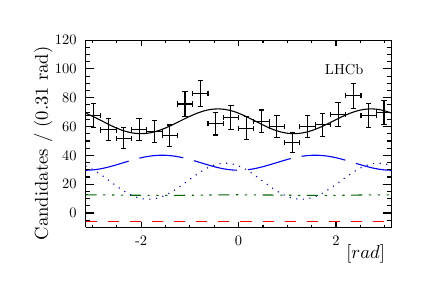
\begin{tikzpicture}
\pgfdeclareplotmark{cross} {
\pgfpathmoveto{\pgfpoint{-0.3\pgfplotmarksize}{\pgfplotmarksize}}
\pgfpathlineto{\pgfpoint{+0.3\pgfplotmarksize}{\pgfplotmarksize}}
\pgfpathlineto{\pgfpoint{+0.3\pgfplotmarksize}{0.3\pgfplotmarksize}}
\pgfpathlineto{\pgfpoint{+1\pgfplotmarksize}{0.3\pgfplotmarksize}}
\pgfpathlineto{\pgfpoint{+1\pgfplotmarksize}{-0.3\pgfplotmarksize}}
\pgfpathlineto{\pgfpoint{+0.3\pgfplotmarksize}{-0.3\pgfplotmarksize}}
\pgfpathlineto{\pgfpoint{+0.3\pgfplotmarksize}{-1.\pgfplotmarksize}}
\pgfpathlineto{\pgfpoint{-0.3\pgfplotmarksize}{-1.\pgfplotmarksize}}
\pgfpathlineto{\pgfpoint{-0.3\pgfplotmarksize}{-0.3\pgfplotmarksize}}
\pgfpathlineto{\pgfpoint{-1.\pgfplotmarksize}{-0.3\pgfplotmarksize}}
\pgfpathlineto{\pgfpoint{-1.\pgfplotmarksize}{0.3\pgfplotmarksize}}
\pgfpathlineto{\pgfpoint{-0.3\pgfplotmarksize}{0.3\pgfplotmarksize}}
\pgfpathclose
\pgfusepathqstroke
}
\pgfdeclareplotmark{cross*} {
\pgfpathmoveto{\pgfpoint{-0.3\pgfplotmarksize}{\pgfplotmarksize}}
\pgfpathlineto{\pgfpoint{+0.3\pgfplotmarksize}{\pgfplotmarksize}}
\pgfpathlineto{\pgfpoint{+0.3\pgfplotmarksize}{0.3\pgfplotmarksize}}
\pgfpathlineto{\pgfpoint{+1\pgfplotmarksize}{0.3\pgfplotmarksize}}
\pgfpathlineto{\pgfpoint{+1\pgfplotmarksize}{-0.3\pgfplotmarksize}}
\pgfpathlineto{\pgfpoint{+0.3\pgfplotmarksize}{-0.3\pgfplotmarksize}}
\pgfpathlineto{\pgfpoint{+0.3\pgfplotmarksize}{-1.\pgfplotmarksize}}
\pgfpathlineto{\pgfpoint{-0.3\pgfplotmarksize}{-1.\pgfplotmarksize}}
\pgfpathlineto{\pgfpoint{-0.3\pgfplotmarksize}{-0.3\pgfplotmarksize}}
\pgfpathlineto{\pgfpoint{-1.\pgfplotmarksize}{-0.3\pgfplotmarksize}}
\pgfpathlineto{\pgfpoint{-1.\pgfplotmarksize}{0.3\pgfplotmarksize}}
\pgfpathlineto{\pgfpoint{-0.3\pgfplotmarksize}{0.3\pgfplotmarksize}}
\pgfpathclose
\pgfusepathqfillstroke
}
\pgfdeclareplotmark{newstar} {
\pgfpathmoveto{\pgfqpoint{0pt}{\pgfplotmarksize}}
\pgfpathlineto{\pgfqpointpolar{44}{0.5\pgfplotmarksize}}
\pgfpathlineto{\pgfqpointpolar{18}{\pgfplotmarksize}}
\pgfpathlineto{\pgfqpointpolar{-20}{0.5\pgfplotmarksize}}
\pgfpathlineto{\pgfqpointpolar{-54}{\pgfplotmarksize}}
\pgfpathlineto{\pgfqpointpolar{-90}{0.5\pgfplotmarksize}}
\pgfpathlineto{\pgfqpointpolar{234}{\pgfplotmarksize}}
\pgfpathlineto{\pgfqpointpolar{198}{0.5\pgfplotmarksize}}
\pgfpathlineto{\pgfqpointpolar{162}{\pgfplotmarksize}}
\pgfpathlineto{\pgfqpointpolar{134}{0.5\pgfplotmarksize}}
\pgfpathclose
\pgfusepathqstroke
}
\pgfdeclareplotmark{newstar*} {
\pgfpathmoveto{\pgfqpoint{0pt}{\pgfplotmarksize}}
\pgfpathlineto{\pgfqpointpolar{44}{0.5\pgfplotmarksize}}
\pgfpathlineto{\pgfqpointpolar{18}{\pgfplotmarksize}}
\pgfpathlineto{\pgfqpointpolar{-20}{0.5\pgfplotmarksize}}
\pgfpathlineto{\pgfqpointpolar{-54}{\pgfplotmarksize}}
\pgfpathlineto{\pgfqpointpolar{-90}{0.5\pgfplotmarksize}}
\pgfpathlineto{\pgfqpointpolar{234}{\pgfplotmarksize}}
\pgfpathlineto{\pgfqpointpolar{198}{0.5\pgfplotmarksize}}
\pgfpathlineto{\pgfqpointpolar{162}{\pgfplotmarksize}}
\pgfpathlineto{\pgfqpointpolar{134}{0.5\pgfplotmarksize}}
\pgfpathclose
\pgfusepathqfillstroke
}
\definecolor{c}{rgb}{1,1,1};
\draw [color=c, fill=c] (0.1,0.0627517) rectangle (4.9,3.07483);
\draw [color=c, fill=c] (0.772,0.544685) rectangle (4.66,2.92423);
\definecolor{c}{rgb}{0,0,0};
\draw [c] (0.772,0.544685) -- (0.772,2.92423) -- (4.66,2.92423) -- (4.66,0.544685) -- (0.772,0.544685);
\definecolor{c}{rgb}{1,1,1};
\draw [color=c, fill=c] (0.772,0.544685) rectangle (4.66,2.92423);
\definecolor{c}{rgb}{0,0,0};
\draw [c] (0.772,0.544685) -- (0.772,2.92423) -- (4.66,2.92423) -- (4.66,0.544685) -- (0.772,0.544685);
\draw [c,line width=0.4] (0.772,0.544685) -- (4.66,0.544685);
\draw [anchor= east] (4.66,0.207332) node[scale=0.672711, rotate=0]{$\phihel [\text{rad}]$};
\draw [c,line width=0.4] (1.47841,0.617878) -- (1.47841,0.544685);
\draw [c,line width=0.4] (1.78781,0.581281) -- (1.78781,0.544685);
\draw [c,line width=0.4] (2.09721,0.581281) -- (2.09721,0.544685);
\draw [c,line width=0.4] (2.4066,0.581281) -- (2.4066,0.544685);
\draw [c,line width=0.4] (2.716,0.617878) -- (2.716,0.544685);
\draw [c,line width=0.4] (3.0254,0.581281) -- (3.0254,0.544685);
\draw [c,line width=0.4] (3.33479,0.581281) -- (3.33479,0.544685);
\draw [c,line width=0.4] (3.64419,0.581281) -- (3.64419,0.544685);
\draw [c,line width=0.4] (3.95359,0.617878) -- (3.95359,0.544685);
\draw [c,line width=0.4] (1.47841,0.617878) -- (1.47841,0.544685);
\draw [c,line width=0.4] (1.16901,0.581281) -- (1.16901,0.544685);
\draw [c,line width=0.4] (0.859617,0.581281) -- (0.859617,0.544685);
\draw [c,line width=0.4] (3.95359,0.617878) -- (3.95359,0.544685);
\draw [c,line width=0.4] (4.26299,0.581281) -- (4.26299,0.544685);
\draw [c,line width=0.4] (4.57238,0.581281) -- (4.57238,0.544685);
\draw [anchor=base] (1.47841,0.321791) node[scale=0.52322, rotate=0]{-2};
\draw [anchor=base] (2.716,0.321791) node[scale=0.52322, rotate=0]{0};
\draw [anchor=base] (3.95359,0.321791) node[scale=0.52322, rotate=0]{2};
\draw [c,line width=0.4] (0.772,2.92423) -- (4.66,2.92423);
\draw [c,line width=0.4] (1.47841,2.85103) -- (1.47841,2.92423);
\draw [c,line width=0.4] (1.78781,2.88763) -- (1.78781,2.92423);
\draw [c,line width=0.4] (2.09721,2.88763) -- (2.09721,2.92423);
\draw [c,line width=0.4] (2.4066,2.88763) -- (2.4066,2.92423);
\draw [c,line width=0.4] (2.716,2.85103) -- (2.716,2.92423);
\draw [c,line width=0.4] (3.0254,2.88763) -- (3.0254,2.92423);
\draw [c,line width=0.4] (3.33479,2.88763) -- (3.33479,2.92423);
\draw [c,line width=0.4] (3.64419,2.88763) -- (3.64419,2.92423);
\draw [c,line width=0.4] (3.95359,2.85103) -- (3.95359,2.92423);
\draw [c,line width=0.4] (1.47841,2.85103) -- (1.47841,2.92423);
\draw [c,line width=0.4] (1.16901,2.88763) -- (1.16901,2.92423);
\draw [c,line width=0.4] (0.859617,2.88763) -- (0.859617,2.92423);
\draw [c,line width=0.4] (3.95359,2.85103) -- (3.95359,2.92423);
\draw [c,line width=0.4] (4.26299,2.88763) -- (4.26299,2.92423);
\draw [c,line width=0.4] (4.57238,2.88763) -- (4.57238,2.92423);
\draw [c,line width=0.4] (0.772,0.544685) -- (0.772,2.92423);
\draw [anchor= east] (0.2344,2.92423) node[scale=0.672711, rotate=90]{Candidates / (0.31 rad)};
\draw [c,line width=0.4] (0.88576,0.727726) -- (0.772,0.727726);
\draw [c,line width=0.4] (0.82888,0.819247) -- (0.772,0.819247);
\draw [c,line width=0.4] (0.82888,0.910768) -- (0.772,0.910768);
\draw [c,line width=0.4] (0.82888,1.00229) -- (0.772,1.00229);
\draw [c,line width=0.4] (0.88576,1.09381) -- (0.772,1.09381);
\draw [c,line width=0.4] (0.82888,1.18533) -- (0.772,1.18533);
\draw [c,line width=0.4] (0.82888,1.27685) -- (0.772,1.27685);
\draw [c,line width=0.4] (0.82888,1.36837) -- (0.772,1.36837);
\draw [c,line width=0.4] (0.88576,1.45989) -- (0.772,1.45989);
\draw [c,line width=0.4] (0.82888,1.55141) -- (0.772,1.55141);
\draw [c,line width=0.4] (0.82888,1.64294) -- (0.772,1.64294);
\draw [c,line width=0.4] (0.82888,1.73446) -- (0.772,1.73446);
\draw [c,line width=0.4] (0.88576,1.82598) -- (0.772,1.82598);
\draw [c,line width=0.4] (0.82888,1.9175) -- (0.772,1.9175);
\draw [c,line width=0.4] (0.82888,2.00902) -- (0.772,2.00902);
\draw [c,line width=0.4] (0.82888,2.10054) -- (0.772,2.10054);
\draw [c,line width=0.4] (0.88576,2.19206) -- (0.772,2.19206);
\draw [c,line width=0.4] (0.82888,2.28358) -- (0.772,2.28358);
\draw [c,line width=0.4] (0.82888,2.3751) -- (0.772,2.3751);
\draw [c,line width=0.4] (0.82888,2.46662) -- (0.772,2.46662);
\draw [c,line width=0.4] (0.88576,2.55814) -- (0.772,2.55814);
\draw [c,line width=0.4] (0.82888,2.64967) -- (0.772,2.64967);
\draw [c,line width=0.4] (0.82888,2.74119) -- (0.772,2.74119);
\draw [c,line width=0.4] (0.82888,2.83271) -- (0.772,2.83271);
\draw [c,line width=0.4] (0.88576,2.92423) -- (0.772,2.92423);
\draw [c,line width=0.4] (0.88576,0.727726) -- (0.772,0.727726);
\draw [c,line width=0.4] (0.82888,0.636205) -- (0.772,0.636205);
\draw [c,line width=0.4] (0.82888,0.544685) -- (0.772,0.544685);
\draw [anchor= east] (0.724,0.727726) node[scale=0.52322, rotate=0]{0};
\draw [anchor= east] (0.724,1.09381) node[scale=0.52322, rotate=0]{20};
\draw [anchor= east] (0.724,1.45989) node[scale=0.52322, rotate=0]{40};
\draw [anchor= east] (0.724,1.82598) node[scale=0.52322, rotate=0]{60};
\draw [anchor= east] (0.724,2.19206) node[scale=0.52322, rotate=0]{80};
\draw [anchor= east] (0.724,2.55814) node[scale=0.52322, rotate=0]{100};
\draw [anchor= east] (0.724,2.92423) node[scale=0.52322, rotate=0]{120};
\draw [c,line width=0.4] (4.66,0.544685) -- (4.66,2.92423);
\draw [c,line width=0.4] (4.54624,0.727726) -- (4.66,0.727726);
\draw [c,line width=0.4] (4.60312,0.819247) -- (4.66,0.819247);
\draw [c,line width=0.4] (4.60312,0.910768) -- (4.66,0.910768);
\draw [c,line width=0.4] (4.60312,1.00229) -- (4.66,1.00229);
\draw [c,line width=0.4] (4.54624,1.09381) -- (4.66,1.09381);
\draw [c,line width=0.4] (4.60312,1.18533) -- (4.66,1.18533);
\draw [c,line width=0.4] (4.60312,1.27685) -- (4.66,1.27685);
\draw [c,line width=0.4] (4.60312,1.36837) -- (4.66,1.36837);
\draw [c,line width=0.4] (4.54624,1.45989) -- (4.66,1.45989);
\draw [c,line width=0.4] (4.60312,1.55141) -- (4.66,1.55141);
\draw [c,line width=0.4] (4.60312,1.64294) -- (4.66,1.64294);
\draw [c,line width=0.4] (4.60312,1.73446) -- (4.66,1.73446);
\draw [c,line width=0.4] (4.54624,1.82598) -- (4.66,1.82598);
\draw [c,line width=0.4] (4.60312,1.9175) -- (4.66,1.9175);
\draw [c,line width=0.4] (4.60312,2.00902) -- (4.66,2.00902);
\draw [c,line width=0.4] (4.60312,2.10054) -- (4.66,2.10054);
\draw [c,line width=0.4] (4.54624,2.19206) -- (4.66,2.19206);
\draw [c,line width=0.4] (4.60312,2.28358) -- (4.66,2.28358);
\draw [c,line width=0.4] (4.60312,2.3751) -- (4.66,2.3751);
\draw [c,line width=0.4] (4.60312,2.46662) -- (4.66,2.46662);
\draw [c,line width=0.4] (4.54624,2.55814) -- (4.66,2.55814);
\draw [c,line width=0.4] (4.60312,2.64967) -- (4.66,2.64967);
\draw [c,line width=0.4] (4.60312,2.74119) -- (4.66,2.74119);
\draw [c,line width=0.4] (4.60312,2.83271) -- (4.66,2.83271);
\draw [c,line width=0.4] (4.54624,2.92423) -- (4.66,2.92423);
\draw [c,line width=0.4] (4.54624,0.727726) -- (4.66,0.727726);
\draw [c,line width=0.4] (4.60312,0.636205) -- (4.66,0.636205);
\draw [c,line width=0.4] (4.60312,0.544685) -- (4.66,0.544685);
\draw [c] (0.8692,1.96341) -- (0.772,1.96341);
\draw [c] (0.772,1.92985) -- (0.772,1.99697);
\draw [c] (0.8692,1.96341) -- (0.9664,1.96341);
\draw [c] (0.9664,1.92985) -- (0.9664,1.99697);
\draw [c] (0.8692,1.96341) -- (0.8692,2.117);
\draw [c] (0.835643,2.117) -- (0.902757,2.117);
\draw [c] (0.8692,1.96341) -- (0.8692,1.80982);
\draw [c] (0.835643,1.80982) -- (0.902757,1.80982);
\draw [c] (1.0636,1.78392) -- (0.9664,1.78392);
\draw [c] (0.9664,1.75037) -- (0.9664,1.81748);
\draw [c] (1.0636,1.78392) -- (1.1608,1.78392);
\draw [c] (1.1608,1.75037) -- (1.1608,1.81748);
\draw [c] (1.0636,1.78392) -- (1.0636,1.92382);
\draw [c] (1.03004,1.92382) -- (1.09716,1.92382);
\draw [c] (1.0636,1.78392) -- (1.0636,1.64403);
\draw [c] (1.03004,1.64403) -- (1.09716,1.64403);
\draw [c] (1.258,1.67889) -- (1.1608,1.67889);
\draw [c] (1.1608,1.64533) -- (1.1608,1.71245);
\draw [c] (1.258,1.67889) -- (1.3552,1.67889);
\draw [c] (1.3552,1.64533) -- (1.3552,1.71245);
\draw [c] (1.258,1.67889) -- (1.258,1.81405);
\draw [c] (1.22444,1.81405) -- (1.29156,1.81405);
\draw [c] (1.258,1.67889) -- (1.258,1.54373);
\draw [c] (1.22444,1.54373) -- (1.29156,1.54373);
\draw [c] (1.4524,1.78673) -- (1.3552,1.78673);
\draw [c] (1.3552,1.75318) -- (1.3552,1.82029);
\draw [c] (1.4524,1.78673) -- (1.5496,1.78673);
\draw [c] (1.5496,1.75318) -- (1.5496,1.82029);
\draw [c] (1.4524,1.78673) -- (1.4524,1.92658);
\draw [c] (1.41884,1.92658) -- (1.48596,1.92658);
\draw [c] (1.4524,1.78673) -- (1.4524,1.64688);
\draw [c] (1.41884,1.64688) -- (1.48596,1.64688);
\draw [c] (1.6468,1.76304) -- (1.5496,1.76304);
\draw [c] (1.5496,1.72948) -- (1.5496,1.7966);
\draw [c] (1.6468,1.76304) -- (1.744,1.76304);
\draw [c] (1.744,1.72948) -- (1.744,1.7966);
\draw [c] (1.6468,1.76304) -- (1.6468,1.90055);
\draw [c] (1.61324,1.90055) -- (1.68036,1.90055);
\draw [c] (1.6468,1.76304) -- (1.6468,1.62553);
\draw [c] (1.61324,1.62553) -- (1.68036,1.62553);
\draw [c] (1.8412,1.70951) -- (1.744,1.70951);
\draw [c] (1.744,1.67595) -- (1.744,1.74306);
\draw [c] (1.8412,1.70951) -- (1.9384,1.70951);
\draw [c] (1.9384,1.67595) -- (1.9384,1.74306);
\draw [c] (1.8412,1.70951) -- (1.8412,1.84596);
\draw [c] (1.80764,1.84596) -- (1.87476,1.84596);
\draw [c] (1.8412,1.70951) -- (1.8412,1.57305);
\draw [c] (1.80764,1.57305) -- (1.87476,1.57305);
\draw [c] (2.0356,2.11235) -- (1.9384,2.11235);
\draw [c] (1.9384,2.07879) -- (1.9384,2.14591);
\draw [c] (2.0356,2.11235) -- (2.1328,2.11235);
\draw [c] (2.1328,2.07879) -- (2.1328,2.14591);
\draw [c] (2.0356,2.11235) -- (2.0356,2.26707);
\draw [c] (2.00204,2.26707) -- (2.06916,2.26707);
\draw [c] (2.0356,2.11235) -- (2.0356,1.95764);
\draw [c] (2.00204,1.95764) -- (2.06916,1.95764);
\draw [c] (2.23,2.24394) -- (2.1328,2.24394);
\draw [c] (2.1328,2.21038) -- (2.1328,2.2775);
\draw [c] (2.23,2.24394) -- (2.3272,2.24394);
\draw [c] (2.3272,2.21038) -- (2.3272,2.2775);
\draw [c] (2.23,2.24394) -- (2.23,2.40814);
\draw [c] (2.19644,2.40814) -- (2.26356,2.40814);
\draw [c] (2.23,2.24394) -- (2.23,2.07974);
\draw [c] (2.19644,2.07974) -- (2.26356,2.07974);
\draw [c] (2.4244,1.86354) -- (2.3272,1.86354);
\draw [c] (2.3272,1.82999) -- (2.3272,1.8971);
\draw [c] (2.4244,1.86354) -- (2.5216,1.86354);
\draw [c] (2.5216,1.82999) -- (2.5216,1.8971);
\draw [c] (2.4244,1.86354) -- (2.4244,2.00843);
\draw [c] (2.39084,2.00843) -- (2.45796,2.00843);
\draw [c] (2.4244,1.86354) -- (2.4244,1.71866);
\draw [c] (2.39084,1.71866) -- (2.45796,1.71866);
\draw [c] (2.6188,1.94512) -- (2.5216,1.94512);
\draw [c] (2.5216,1.91156) -- (2.5216,1.97867);
\draw [c] (2.6188,1.94512) -- (2.716,1.94512);
\draw [c] (2.716,1.91156) -- (2.716,1.97867);
\draw [c] (2.6188,1.94512) -- (2.6188,2.09682);
\draw [c] (2.58524,2.09682) -- (2.65236,2.09682);
\draw [c] (2.6188,1.94512) -- (2.6188,1.79341);
\draw [c] (2.58524,1.79341) -- (2.65236,1.79341);
\draw [c] (2.8132,1.80577) -- (2.716,1.80577);
\draw [c] (2.716,1.77221) -- (2.716,1.83932);
\draw [c] (2.8132,1.80577) -- (2.9104,1.80577);
\draw [c] (2.9104,1.77221) -- (2.9104,1.83932);
\draw [c] (2.8132,1.80577) -- (2.8132,1.94954);
\draw [c] (2.77964,1.94954) -- (2.84676,1.94954);
\draw [c] (2.8132,1.80577) -- (2.8132,1.66199);
\draw [c] (2.77964,1.66199) -- (2.84676,1.66199);
\draw [c] (3.0076,1.89231) -- (2.9104,1.89231);
\draw [c] (2.9104,1.85875) -- (2.9104,1.92586);
\draw [c] (3.0076,1.89231) -- (3.1048,1.89231);
\draw [c] (3.1048,1.85875) -- (3.1048,1.92586);
\draw [c] (3.0076,1.89231) -- (3.0076,2.03691);
\draw [c] (2.97404,2.03691) -- (3.04116,2.03691);
\draw [c] (3.0076,1.89231) -- (3.0076,1.74771);
\draw [c] (2.97404,1.74771) -- (3.04116,1.74771);
\draw [c] (3.202,1.83062) -- (3.1048,1.83062);
\draw [c] (3.1048,1.79706) -- (3.1048,1.86418);
\draw [c] (3.202,1.83062) -- (3.2992,1.83062);
\draw [c] (3.2992,1.79706) -- (3.2992,1.86418);
\draw [c] (3.202,1.83062) -- (3.202,1.97006);
\draw [c] (3.16844,1.97006) -- (3.23556,1.97006);
\draw [c] (3.202,1.83062) -- (3.202,1.69118);
\draw [c] (3.16844,1.69118) -- (3.23556,1.69118);
\draw [c] (3.3964,1.62415) -- (3.2992,1.62415);
\draw [c] (3.2992,1.5906) -- (3.2992,1.65771);
\draw [c] (3.3964,1.62415) -- (3.4936,1.62415);
\draw [c] (3.4936,1.5906) -- (3.4936,1.65771);
\draw [c] (3.3964,1.62415) -- (3.3964,1.75548);
\draw [c] (3.36284,1.75548) -- (3.42996,1.75548);
\draw [c] (3.3964,1.62415) -- (3.3964,1.49283);
\draw [c] (3.36284,1.49283) -- (3.42996,1.49283);
\draw [c] (3.5908,1.8249) -- (3.4936,1.8249);
\draw [c] (3.4936,1.79135) -- (3.4936,1.85846);
\draw [c] (3.5908,1.8249) -- (3.688,1.8249);
\draw [c] (3.688,1.79135) -- (3.688,1.85846);
\draw [c] (3.5908,1.8249) -- (3.5908,1.96821);
\draw [c] (3.55724,1.96821) -- (3.62436,1.96821);
\draw [c] (3.5908,1.8249) -- (3.5908,1.6816);
\draw [c] (3.55724,1.6816) -- (3.62436,1.6816);
\draw [c] (3.7852,1.84784) -- (3.688,1.84784);
\draw [c] (3.688,1.81429) -- (3.688,1.8814);
\draw [c] (3.7852,1.84784) -- (3.8824,1.84784);
\draw [c] (3.8824,1.81429) -- (3.8824,1.8814);
\draw [c] (3.7852,1.84784) -- (3.7852,1.99152);
\draw [c] (3.75164,1.99152) -- (3.81876,1.99152);
\draw [c] (3.7852,1.84784) -- (3.7852,1.70417);
\draw [c] (3.75164,1.70417) -- (3.81876,1.70417);
\draw [c] (3.9796,1.97861) -- (3.8824,1.97861);
\draw [c] (3.8824,1.94505) -- (3.8824,2.01217);
\draw [c] (3.9796,1.97861) -- (4.0768,1.97861);
\draw [c] (4.0768,1.94505) -- (4.0768,2.01217);
\draw [c] (3.9796,1.97861) -- (3.9796,2.12764);
\draw [c] (3.94604,2.12764) -- (4.01316,2.12764);
\draw [c] (3.9796,1.97861) -- (3.9796,1.82958);
\draw [c] (3.94604,1.82958) -- (4.01316,1.82958);
\draw [c] (4.174,2.21803) -- (4.0768,2.21803);
\draw [c] (4.0768,2.18447) -- (4.0768,2.25158);
\draw [c] (4.174,2.21803) -- (4.2712,2.21803);
\draw [c] (4.2712,2.18447) -- (4.2712,2.25158);
\draw [c] (4.174,2.21803) -- (4.174,2.37723);
\draw [c] (4.14044,2.37723) -- (4.20756,2.37723);
\draw [c] (4.174,2.21803) -- (4.174,2.05882);
\draw [c] (4.14044,2.05882) -- (4.20756,2.05882);
\draw [c] (4.3684,1.96615) -- (4.2712,1.96615);
\draw [c] (4.2712,1.93259) -- (4.2712,1.9997);
\draw [c] (4.3684,1.96615) -- (4.4656,1.96615);
\draw [c] (4.4656,1.93259) -- (4.4656,1.9997);
\draw [c] (4.3684,1.96615) -- (4.3684,2.11572);
\draw [c] (4.33484,2.11572) -- (4.40196,2.11572);
\draw [c] (4.3684,1.96615) -- (4.3684,1.81658);
\draw [c] (4.33484,1.81658) -- (4.40196,1.81658);
\draw [c] (4.5628,2.00459) -- (4.4656,2.00459);
\draw [c] (4.4656,1.97103) -- (4.4656,2.03814);
\draw [c] (4.5628,2.00459) -- (4.66,2.00459);
\draw [c] (4.66,1.97103) -- (4.66,2.03814);
\draw [c] (4.5628,2.00459) -- (4.5628,2.15785);
\draw [c] (4.52924,2.15785) -- (4.59636,2.15785);
\draw [c] (4.5628,2.00459) -- (4.5628,1.85132);
\draw [c] (4.52924,1.85132) -- (4.59636,1.85132);
\foreach \P in
 {(0.8692,1.96341),(1.0636,1.78392),(1.258,1.67889),(1.4524,1.78673),(1.6468,1.76304),(1.8412,1.70951),(2.0356,2.11235),(2.23,2.24394),(2.4244,1.86354),(2.6188,1.94512),(2.8132,1.80577),(3.0076,1.89231),(3.202,1.83062),(3.3964,1.62415),(3.5908,1.8249
),(3.7852,1.84784),(3.9796,1.97861),(4.174,2.21803),(4.3684,1.96615),(4.5628,2.00459)}{\draw[mark options={color=c,fill=c},mark size=1.201201pt,mark=] plot coordinates {\P};}
\definecolor{c}{rgb}{1,0,0};
\draw [c,dash pattern=on 4pt off 4pt] (0.772,0.622545) -- (0.772,0.622545);
\draw [c,dash pattern=on 4pt off 4pt] (0.772,0.622545) -- (0.9664,0.622545) -- (1.1608,0.622545) -- (1.3552,0.622545) -- (1.5496,0.622545) -- (1.744,0.622545) -- (1.9384,0.622545) -- (2.1328,0.622545) -- (2.3272,0.622545) -- (2.5216,0.622545) --
 (2.716,0.622545) -- (2.9104,0.622545) -- (3.1048,0.622545) -- (3.2992,0.622545) -- (3.4936,0.622545) -- (3.688,0.622545) -- (3.8824,0.622545) -- (4.0768,0.622545) -- (4.2712,0.622545) -- (4.4656,0.622545) -- (4.66,0.622545) -- (4.66,0.622545) --
 (4.66,0.622545);
\definecolor{c}{rgb}{0,0.4,0};
\draw [c,dash pattern=on 4pt off 2.4pt on 0.8pt off 2.4pt on 0.8pt off 2.4pt on 0.8pt off 2.4pt] (0.772,0.959345) -- (0.772,0.959345);
\draw [c,dash pattern=on 4pt off 2.4pt on 0.8pt off 2.4pt on 0.8pt off 2.4pt on 0.8pt off 2.4pt] (0.772,0.959345) -- (0.7963,0.959333) -- (0.8206,0.959297) -- (0.8449,0.959236) -- (0.8692,0.959152) -- (0.8935,0.959045) -- (0.9178,0.958916) --
 (0.9421,0.958765) -- (0.9664,0.958593) -- (0.9907,0.958401) -- (1.015,0.958191) -- (1.0393,0.957964) -- (1.0636,0.957721) -- (1.1122,0.957194) -- (1.1608,0.956623) -- (1.3552,0.954188) -- (1.4038,0.953617) -- (1.4524,0.953089) -- (1.4767,0.952847)
 -- (1.501,0.952619) -- (1.5253,0.952409) -- (1.5496,0.952218) -- (1.5739,0.952046) -- (1.5982,0.951895) -- (1.6225,0.951765) -- (1.6468,0.951658) -- (1.6711,0.951574) -- (1.6954,0.951514) -- (1.7197,0.951478) -- (1.744,0.951465) -- (1.7683,0.951478)
 -- (1.7926,0.951514) -- (1.8169,0.951574) -- (1.8412,0.951658) -- (1.8655,0.951765) -- (1.8898,0.951895) -- (1.9141,0.952046) -- (1.9384,0.952218) -- (1.9627,0.952409) -- (1.987,0.952619) -- (2.0113,0.952847) -- (2.0356,0.953089) --
 (2.0842,0.953617) -- (2.1328,0.954188) -- (2.3272,0.956623) -- (2.3758,0.957194) -- (2.4244,0.957721) -- (2.4487,0.957964) -- (2.473,0.958191) -- (2.4973,0.958401) -- (2.5216,0.958593) -- (2.5459,0.958765) -- (2.5702,0.958916) -- (2.5945,0.959045)
 -- (2.6188,0.959152) -- (2.6431,0.959236) -- (2.6674,0.959297) -- (2.6917,0.959333) -- (2.716,0.959345) -- (2.7403,0.959333) -- (2.7646,0.959297) -- (2.7889,0.959236) -- (2.8132,0.959152) -- (2.8375,0.959045) -- (2.8618,0.958916) --
 (2.8861,0.958765) -- (2.9104,0.958593) -- (2.9347,0.958401) -- (2.959,0.958191) -- (2.9833,0.957964) -- (3.0076,0.957721) -- (3.0562,0.957194) -- (3.1048,0.956623) -- (3.2992,0.954188) -- (3.3478,0.953617) -- (3.3964,0.953089) -- (3.4207,0.952847)
 -- (3.445,0.952619) -- (3.4693,0.952409) -- (3.4936,0.952218) -- (3.5179,0.952046) -- (3.5422,0.951895) -- (3.5665,0.951765) -- (3.5908,0.951658) -- (3.6151,0.951574) -- (3.6394,0.951514) -- (3.6637,0.951478) -- (3.688,0.951465) -- (3.7123,0.951478)
 -- (3.7366,0.951514) -- (3.7609,0.951574) -- (3.7852,0.951658) -- (3.8095,0.951765) -- (3.8338,0.951895) -- (3.8581,0.952046) -- (3.8824,0.952218) -- (3.9067,0.952409) -- (3.931,0.952619) -- (3.9553,0.952847) -- (3.9796,0.953089) --
 (4.0282,0.953617) -- (4.0768,0.954188) -- (4.2712,0.956623) -- (4.3198,0.957194) -- (4.3684,0.957721) -- (4.3927,0.957964) -- (4.417,0.958191) -- (4.4413,0.958401) -- (4.4656,0.958593) -- (4.4899,0.958765) -- (4.5142,0.958916) -- (4.5385,0.959045)
 -- (4.5628,0.959152) -- (4.5871,0.959236) -- (4.6114,0.959297) -- (4.6357,0.959333) -- (4.66,0.959345) -- (4.66,0.959345) -- (4.66,0.959345);
\definecolor{c}{rgb}{0,0,1};
\draw [c,dotted] (0.772,1.32623) -- (0.772,1.32623);
\draw [c,dotted] (0.772,1.32623) -- (0.7963,1.31602) -- (0.8206,1.30463) -- (0.8449,1.29213) -- (0.8692,1.27862) -- (0.9178,1.24888) -- (0.9664,1.2162) -- (1.015,1.18143) -- (1.0636,1.14547) -- (1.1608,1.07364) -- (1.2094,1.03959) -- (1.258,1.00791)
 -- (1.3066,0.979361) -- (1.3309,0.966474) -- (1.3552,0.954615) -- (1.3795,0.943851) -- (1.4038,0.934242) -- (1.4281,0.925843) -- (1.4524,0.918698) -- (1.4767,0.912845) -- (1.501,0.908316) -- (1.5253,0.905132) -- (1.5496,0.903309) --
 (1.5739,0.902852) -- (1.5982,0.903762) -- (1.6225,0.90603) -- (1.6468,0.909639) -- (1.6711,0.914568) -- (1.6954,0.920785) -- (1.7197,0.928253) -- (1.744,0.936928) -- (1.7683,0.946759) -- (1.7926,0.957689) -- (1.8169,0.969655) -- (1.8412,0.982587) --
 (1.8898,1.01105) -- (1.9384,1.04242) -- (1.987,1.07598) -- (2.0356,1.11095) -- (2.1328,1.18177) -- (2.1814,1.21591) -- (2.23,1.24809) -- (2.2786,1.27748) -- (2.3029,1.2909) -- (2.3272,1.30334) -- (2.3515,1.31473) -- (2.3758,1.32498) --
 (2.4001,1.33404) -- (2.4244,1.34183) -- (2.4487,1.34831) -- (2.473,1.35343) -- (2.4973,1.35714) -- (2.5216,1.35943) -- (2.5459,1.36028) -- (2.5702,1.35967) -- (2.5945,1.35761) -- (2.6188,1.35411) -- (2.6431,1.34918) -- (2.6674,1.34287) --
 (2.6917,1.3352) -- (2.716,1.32623) -- (2.7403,1.31602) -- (2.7646,1.30463) -- (2.7889,1.29213) -- (2.8132,1.27862) -- (2.8618,1.24888) -- (2.9104,1.2162) -- (2.959,1.18143) -- (3.0076,1.14547) -- (3.1048,1.07364) -- (3.1534,1.03959) --
 (3.202,1.00791) -- (3.2506,0.979361) -- (3.2749,0.966474) -- (3.2992,0.954615) -- (3.3235,0.943851) -- (3.3478,0.934242) -- (3.3721,0.925843) -- (3.3964,0.918698) -- (3.4207,0.912845) -- (3.445,0.908316) -- (3.4693,0.905132) -- (3.4936,0.903309) --
 (3.5179,0.902852) -- (3.5422,0.903762) -- (3.5665,0.90603) -- (3.5908,0.909639) -- (3.6151,0.914568) -- (3.6394,0.920785) -- (3.6637,0.928253) -- (3.688,0.936928) -- (3.7123,0.946759) -- (3.7366,0.957689) -- (3.7609,0.969655) -- (3.7852,0.982587) --
 (3.8338,1.01105) -- (3.8824,1.04242) -- (3.931,1.07598) -- (3.9796,1.11095) -- (4.0768,1.18177) -- (4.1254,1.21591) -- (4.174,1.24809) -- (4.2226,1.27748) -- (4.2469,1.2909) -- (4.2712,1.30334) -- (4.2955,1.31473) -- (4.3198,1.32498) --
 (4.3441,1.33404) -- (4.3684,1.34183) -- (4.3927,1.34831) -- (4.417,1.35343) -- (4.4413,1.35714) -- (4.4656,1.35943) -- (4.4899,1.36028) -- (4.5142,1.35967) -- (4.5385,1.35761) -- (4.5628,1.35411) -- (4.5871,1.34918) -- (4.6114,1.34287) --
 (4.6357,1.3352) -- (4.66,1.32623) -- (4.66,1.32623) -- (4.66,1.32623);
\draw [c,dash pattern=on 16pt off 4pt] (0.772,1.27147) -- (0.772,1.27147);
\draw [c,dash pattern=on 16pt off 4pt] (0.772,1.27147) -- (0.7963,1.27177) -- (0.8206,1.27269) -- (0.8449,1.2742) -- (0.8692,1.27631) -- (0.8935,1.279) -- (0.9178,1.28224) -- (0.9421,1.28602) -- (0.9664,1.29031) -- (0.9907,1.29508) -- (1.015,1.30031)
 -- (1.0636,1.31196) -- (1.1122,1.32496) -- (1.1608,1.33897) -- (1.3552,1.3978) -- (1.4038,1.41139) -- (1.4524,1.42385) -- (1.4767,1.42958) -- (1.501,1.43491) -- (1.5253,1.43984) -- (1.5496,1.44432) -- (1.5739,1.44833) -- (1.5982,1.45185) --
 (1.6225,1.45487) -- (1.6468,1.45736) -- (1.6711,1.45931) -- (1.6954,1.46071) -- (1.7197,1.46155) -- (1.744,1.46183) -- (1.7683,1.46155) -- (1.7926,1.46071) -- (1.8169,1.45931) -- (1.8412,1.45736) -- (1.8655,1.45487) -- (1.8898,1.45185) --
 (1.9141,1.44833) -- (1.9384,1.44432) -- (1.9627,1.43984) -- (1.987,1.43491) -- (2.0113,1.42958) -- (2.0356,1.42385) -- (2.0842,1.41139) -- (2.1328,1.3978) -- (2.3272,1.33897) -- (2.3758,1.32496) -- (2.4244,1.31196) -- (2.473,1.30031) --
 (2.4973,1.29508) -- (2.5216,1.29031) -- (2.5459,1.28602) -- (2.5702,1.28224) -- (2.5945,1.279) -- (2.6188,1.27631) -- (2.6431,1.2742) -- (2.6674,1.27269) -- (2.6917,1.27177) -- (2.716,1.27147) -- (2.7403,1.27177) -- (2.7646,1.27269) --
 (2.7889,1.2742) -- (2.8132,1.27631) -- (2.8375,1.279) -- (2.8618,1.28224) -- (2.8861,1.28602) -- (2.9104,1.29031) -- (2.9347,1.29508) -- (2.959,1.30031) -- (3.0076,1.31196) -- (3.0562,1.32496) -- (3.1048,1.33897) -- (3.2992,1.3978) --
 (3.3478,1.41139) -- (3.3964,1.42385) -- (3.4207,1.42958) -- (3.445,1.43491) -- (3.4693,1.43984) -- (3.4936,1.44432) -- (3.5179,1.44833) -- (3.5422,1.45185) -- (3.5665,1.45487) -- (3.5908,1.45736) -- (3.6151,1.45931) -- (3.6394,1.46071) --
 (3.6637,1.46155) -- (3.688,1.46183) -- (3.7123,1.46155) -- (3.7366,1.46071) -- (3.7609,1.45931) -- (3.7852,1.45736) -- (3.8095,1.45487) -- (3.8338,1.45185) -- (3.8581,1.44833) -- (3.8824,1.44432) -- (3.9067,1.43984) -- (3.931,1.43491) --
 (3.9553,1.42958) -- (3.9796,1.42385) -- (4.0282,1.41139) -- (4.0768,1.3978) -- (4.2712,1.33897) -- (4.3198,1.32496) -- (4.3684,1.31196) -- (4.417,1.30031) -- (4.4413,1.29508) -- (4.4656,1.29031) -- (4.4899,1.28602) -- (4.5142,1.28224) --
 (4.5385,1.279) -- (4.5628,1.27631) -- (4.5871,1.2742) -- (4.6114,1.27269) -- (4.6357,1.27177) -- (4.66,1.27147) -- (4.66,1.27147) -- (4.66,1.27147);
\definecolor{c}{rgb}{0,0,0};
\draw [c] (0.772,1.99565) -- (0.772,1.99565);
\draw [c] (0.772,1.99565) -- (0.8206,1.9754) -- (0.8692,1.95307) -- (0.9178,1.92922) -- (0.9664,1.90449) -- (1.0636,1.85491) -- (1.1122,1.83133) -- (1.1608,1.80935) -- (1.2094,1.78951) -- (1.2337,1.78054) -- (1.258,1.77228) -- (1.2823,1.76478) --
 (1.3066,1.75808) -- (1.3309,1.75222) -- (1.3552,1.74723) -- (1.3795,1.74313) -- (1.4038,1.73995) -- (1.4281,1.7377) -- (1.4524,1.73639) -- (1.4767,1.73603) -- (1.501,1.73662) -- (1.5253,1.73814) -- (1.5496,1.7406) -- (1.5739,1.74396) --
 (1.5982,1.74822) -- (1.6225,1.75333) -- (1.6468,1.75927) -- (1.6711,1.76601) -- (1.6954,1.7735) -- (1.7197,1.7817) -- (1.744,1.79056) -- (1.7926,1.81006) -- (1.8412,1.83154) -- (1.8898,1.8545) -- (1.9384,1.87841) -- (2.0356,1.92683) --
 (2.0842,1.95019) -- (2.1328,1.97223) -- (2.1814,1.9924) -- (2.2057,2.00162) -- (2.23,2.01019) -- (2.2543,2.01804) -- (2.2786,2.02514) -- (2.3029,2.03143) -- (2.3272,2.03686) -- (2.3515,2.0414) -- (2.3758,2.04502) -- (2.4001,2.0477) --
 (2.4244,2.0494) -- (2.4487,2.05013) -- (2.473,2.04986) -- (2.4973,2.0486) -- (2.5216,2.04635) -- (2.5459,2.04313) -- (2.5702,2.03895) -- (2.5945,2.03384) -- (2.6188,2.02784) -- (2.6431,2.02097) -- (2.6674,2.01328) -- (2.6917,2.00482) --
 (2.716,1.99565) -- (2.7646,1.9754) -- (2.8132,1.95307) -- (2.8618,1.92922) -- (2.9104,1.90449) -- (3.0076,1.85491) -- (3.0562,1.83133) -- (3.1048,1.80935) -- (3.1534,1.78951) -- (3.1777,1.78054) -- (3.202,1.77228) -- (3.2263,1.76478) --
 (3.2506,1.75808) -- (3.2749,1.75222) -- (3.2992,1.74723) -- (3.3235,1.74313) -- (3.3478,1.73995) -- (3.3721,1.7377) -- (3.3964,1.73639) -- (3.4207,1.73603) -- (3.445,1.73662) -- (3.4693,1.73814) -- (3.4936,1.7406) -- (3.5179,1.74396) --
 (3.5422,1.74822) -- (3.5665,1.75333) -- (3.5908,1.75927) -- (3.6151,1.76601) -- (3.6394,1.7735) -- (3.6637,1.7817) -- (3.688,1.79056) -- (3.7366,1.81006) -- (3.7852,1.83154) -- (3.8338,1.8545) -- (3.8824,1.87841) -- (3.9796,1.92683) --
 (4.0282,1.95019) -- (4.0768,1.97223) -- (4.1254,1.9924) -- (4.1497,2.00162) -- (4.174,2.01019) -- (4.1983,2.01804) -- (4.2226,2.02514) -- (4.2469,2.03143) -- (4.2712,2.03686) -- (4.2955,2.0414) -- (4.3198,2.04502) -- (4.3441,2.0477) --
 (4.3684,2.0494) -- (4.3927,2.05013) -- (4.417,2.04986) -- (4.4413,2.0486) -- (4.4656,2.04635) -- (4.4899,2.04313) -- (4.5142,2.03895) -- (4.5385,2.03384) -- (4.5628,2.02784) -- (4.5871,2.02097) -- (4.6114,2.01328) -- (4.6357,2.00482) --
 (4.66,1.99565) -- (4.66,1.99565) -- (4.66,1.99565);
\draw [c,line width=0.4] (0.772,0.544685) -- (4.66,0.544685);
\draw [c,line width=0.4] (1.47841,0.617878) -- (1.47841,0.544685);
\draw [c,line width=0.4] (1.78781,0.581281) -- (1.78781,0.544685);
\draw [c,line width=0.4] (2.09721,0.581281) -- (2.09721,0.544685);
\draw [c,line width=0.4] (2.4066,0.581281) -- (2.4066,0.544685);
\draw [c,line width=0.4] (2.716,0.617878) -- (2.716,0.544685);
\draw [c,line width=0.4] (3.0254,0.581281) -- (3.0254,0.544685);
\draw [c,line width=0.4] (3.33479,0.581281) -- (3.33479,0.544685);
\draw [c,line width=0.4] (3.64419,0.581281) -- (3.64419,0.544685);
\draw [c,line width=0.4] (3.95359,0.617878) -- (3.95359,0.544685);
\draw [c,line width=0.4] (1.47841,0.617878) -- (1.47841,0.544685);
\draw [c,line width=0.4] (1.16901,0.581281) -- (1.16901,0.544685);
\draw [c,line width=0.4] (0.859617,0.581281) -- (0.859617,0.544685);
\draw [c,line width=0.4] (3.95359,0.617878) -- (3.95359,0.544685);
\draw [c,line width=0.4] (4.26299,0.581281) -- (4.26299,0.544685);
\draw [c,line width=0.4] (4.57238,0.581281) -- (4.57238,0.544685);
\draw [c,line width=0.4] (0.772,2.92423) -- (4.66,2.92423);
\draw [c,line width=0.4] (1.47841,2.85103) -- (1.47841,2.92423);
\draw [c,line width=0.4] (1.78781,2.88763) -- (1.78781,2.92423);
\draw [c,line width=0.4] (2.09721,2.88763) -- (2.09721,2.92423);
\draw [c,line width=0.4] (2.4066,2.88763) -- (2.4066,2.92423);
\draw [c,line width=0.4] (2.716,2.85103) -- (2.716,2.92423);
\draw [c,line width=0.4] (3.0254,2.88763) -- (3.0254,2.92423);
\draw [c,line width=0.4] (3.33479,2.88763) -- (3.33479,2.92423);
\draw [c,line width=0.4] (3.64419,2.88763) -- (3.64419,2.92423);
\draw [c,line width=0.4] (3.95359,2.85103) -- (3.95359,2.92423);
\draw [c,line width=0.4] (1.47841,2.85103) -- (1.47841,2.92423);
\draw [c,line width=0.4] (1.16901,2.88763) -- (1.16901,2.92423);
\draw [c,line width=0.4] (0.859617,2.88763) -- (0.859617,2.92423);
\draw [c,line width=0.4] (3.95359,2.85103) -- (3.95359,2.92423);
\draw [c,line width=0.4] (4.26299,2.88763) -- (4.26299,2.92423);
\draw [c,line width=0.4] (4.57238,2.88763) -- (4.57238,2.92423);
\draw [c,line width=0.4] (0.772,0.544685) -- (0.772,2.92423);
\draw [c,line width=0.4] (0.88576,0.727726) -- (0.772,0.727726);
\draw [c,line width=0.4] (0.82888,0.819247) -- (0.772,0.819247);
\draw [c,line width=0.4] (0.82888,0.910768) -- (0.772,0.910768);
\draw [c,line width=0.4] (0.82888,1.00229) -- (0.772,1.00229);
\draw [c,line width=0.4] (0.88576,1.09381) -- (0.772,1.09381);
\draw [c,line width=0.4] (0.82888,1.18533) -- (0.772,1.18533);
\draw [c,line width=0.4] (0.82888,1.27685) -- (0.772,1.27685);
\draw [c,line width=0.4] (0.82888,1.36837) -- (0.772,1.36837);
\draw [c,line width=0.4] (0.88576,1.45989) -- (0.772,1.45989);
\draw [c,line width=0.4] (0.82888,1.55141) -- (0.772,1.55141);
\draw [c,line width=0.4] (0.82888,1.64294) -- (0.772,1.64294);
\draw [c,line width=0.4] (0.82888,1.73446) -- (0.772,1.73446);
\draw [c,line width=0.4] (0.88576,1.82598) -- (0.772,1.82598);
\draw [c,line width=0.4] (0.82888,1.9175) -- (0.772,1.9175);
\draw [c,line width=0.4] (0.82888,2.00902) -- (0.772,2.00902);
\draw [c,line width=0.4] (0.82888,2.10054) -- (0.772,2.10054);
\draw [c,line width=0.4] (0.88576,2.19206) -- (0.772,2.19206);
\draw [c,line width=0.4] (0.82888,2.28358) -- (0.772,2.28358);
\draw [c,line width=0.4] (0.82888,2.3751) -- (0.772,2.3751);
\draw [c,line width=0.4] (0.82888,2.46662) -- (0.772,2.46662);
\draw [c,line width=0.4] (0.88576,2.55814) -- (0.772,2.55814);
\draw [c,line width=0.4] (0.82888,2.64967) -- (0.772,2.64967);
\draw [c,line width=0.4] (0.82888,2.74119) -- (0.772,2.74119);
\draw [c,line width=0.4] (0.82888,2.83271) -- (0.772,2.83271);
\draw [c,line width=0.4] (0.88576,2.92423) -- (0.772,2.92423);
\draw [c,line width=0.4] (0.88576,0.727726) -- (0.772,0.727726);
\draw [c,line width=0.4] (0.82888,0.636205) -- (0.772,0.636205);
\draw [c,line width=0.4] (0.82888,0.544685) -- (0.772,0.544685);
\draw [c,line width=0.4] (4.66,0.544685) -- (4.66,2.92423);
\draw [c,line width=0.4] (4.54624,0.727726) -- (4.66,0.727726);
\draw [c,line width=0.4] (4.60312,0.819247) -- (4.66,0.819247);
\draw [c,line width=0.4] (4.60312,0.910768) -- (4.66,0.910768);
\draw [c,line width=0.4] (4.60312,1.00229) -- (4.66,1.00229);
\draw [c,line width=0.4] (4.54624,1.09381) -- (4.66,1.09381);
\draw [c,line width=0.4] (4.60312,1.18533) -- (4.66,1.18533);
\draw [c,line width=0.4] (4.60312,1.27685) -- (4.66,1.27685);
\draw [c,line width=0.4] (4.60312,1.36837) -- (4.66,1.36837);
\draw [c,line width=0.4] (4.54624,1.45989) -- (4.66,1.45989);
\draw [c,line width=0.4] (4.60312,1.55141) -- (4.66,1.55141);
\draw [c,line width=0.4] (4.60312,1.64294) -- (4.66,1.64294);
\draw [c,line width=0.4] (4.60312,1.73446) -- (4.66,1.73446);
\draw [c,line width=0.4] (4.54624,1.82598) -- (4.66,1.82598);
\draw [c,line width=0.4] (4.60312,1.9175) -- (4.66,1.9175);
\draw [c,line width=0.4] (4.60312,2.00902) -- (4.66,2.00902);
\draw [c,line width=0.4] (4.60312,2.10054) -- (4.66,2.10054);
\draw [c,line width=0.4] (4.54624,2.19206) -- (4.66,2.19206);
\draw [c,line width=0.4] (4.60312,2.28358) -- (4.66,2.28358);
\draw [c,line width=0.4] (4.60312,2.3751) -- (4.66,2.3751);
\draw [c,line width=0.4] (4.60312,2.46662) -- (4.66,2.46662);
\draw [c,line width=0.4] (4.54624,2.55814) -- (4.66,2.55814);
\draw [c,line width=0.4] (4.60312,2.64967) -- (4.66,2.64967);
\draw [c,line width=0.4] (4.60312,2.74119) -- (4.66,2.74119);
\draw [c,line width=0.4] (4.60312,2.83271) -- (4.66,2.83271);
\draw [c,line width=0.4] (4.54624,2.92423) -- (4.66,2.92423);
\draw [c,line width=0.4] (4.54624,0.727726) -- (4.66,0.727726);
\draw [c,line width=0.4] (4.60312,0.636205) -- (4.66,0.636205);
\draw [c,line width=0.4] (4.60312,0.544685) -- (4.66,0.544685);
\draw [anchor= west] (3.748,2.54772) node[scale=0.52322, rotate=0]{LHCb};
\end{tikzpicture}
}
    \caption{}
    \label{angPlot_phi}
  \end{subfigure}
  \caption{Fitted angular pdf projections on top of the \BsJpsiKst sWeighted data. 
           Black solid: total, blue dashed \pwave even, blue dotted \pwave odd plus \pwave self interference, 
           green dotted: \swave, red dotted dashed S-P interference. Notice the negative values of the \spwave interverence.
           Pull distributions are shown as well.}
  \label{angular_plot}
\end{center}
\end{figure}


\begin{table}[!h]
  \center
  \begin{tabular}{c c c}
    \hline
     parameter & value & statistical uncertainty \\
     \hline
     $             \Acp{0}$ & $-0.063$ & $(+0.063,-0.063)$ \\
     $     \Acp{\parallel}$ & $+0.155$ & $(+0.159,-0.157)$ \\
     $         \Acp{\perp}$ & $-0.087$ & $(+0.097,-0.097)$ \\
     $             \Acp{S}$ & $+0.129$ & $(+0.098,-0.097)$ \\
     \hline
     $              \fP{0}$ & $+0.481$ & $(+0.024,-0.025)$ \\
     $      \fP{\parallel}$ & $+0.183$ & $(+0.028,-0.027)$ \\
     $\ampPhase{\parallel}$ & $-2.766$ & $(+0.163,-0.166)$ \\
     $    \ampPhase{\perp}$ & $-0.067$ & $(+0.113,-0.116)$ \\
     \hline
     $              \fS{1}$ & $+0.567$ & $(+0.066,-0.077)$ \\
     $              \fS{2}$ & $+0.098$ & $(+0.034,-0.027)$ \\
     $              \fS{3}$ & $+0.045$ & $(+0.045,-0.030)$ \\
     $              \fS{4}$ & $+0.578$ & $(+0.111,-0.120)$ \\
     $          \deltaS{1}$ & $+0.265$ & $(+0.136,-0.131)$ \\
     $          \deltaS{2}$ & $-0.532$ & $(+0.229,-0.195)$ \\
     $          \deltaS{3}$ & $-1.682$ & $(+0.189,-0.240)$ \\
     $          \deltaS{4}$ & $-2.070$ & $(+0.142,-0.160)$ \\
    \hline
  \end{tabular}
  \caption{\small Best fit values of the parameters of intereset.}
  \label{bestFitResult}
\end{table}

%% \begin{figure}[h]
%%   \centering
%%   \begin{subfigure}{0.5\textwidth}
%%     \tikzsetnextfilename{pW_wave_yields}
%%     \scalebox{0.60}{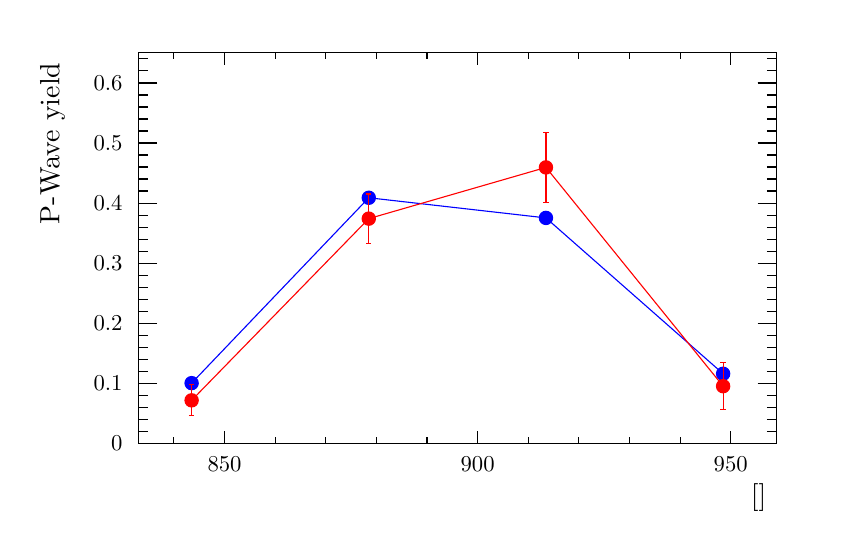
\begin{tikzpicture}
\pgfdeclareplotmark{cross} {
\pgfpathmoveto{\pgfpoint{-0.3\pgfplotmarksize}{\pgfplotmarksize}}
\pgfpathlineto{\pgfpoint{+0.3\pgfplotmarksize}{\pgfplotmarksize}}
\pgfpathlineto{\pgfpoint{+0.3\pgfplotmarksize}{0.3\pgfplotmarksize}}
\pgfpathlineto{\pgfpoint{+1\pgfplotmarksize}{0.3\pgfplotmarksize}}
\pgfpathlineto{\pgfpoint{+1\pgfplotmarksize}{-0.3\pgfplotmarksize}}
\pgfpathlineto{\pgfpoint{+0.3\pgfplotmarksize}{-0.3\pgfplotmarksize}}
\pgfpathlineto{\pgfpoint{+0.3\pgfplotmarksize}{-1.\pgfplotmarksize}}
\pgfpathlineto{\pgfpoint{-0.3\pgfplotmarksize}{-1.\pgfplotmarksize}}
\pgfpathlineto{\pgfpoint{-0.3\pgfplotmarksize}{-0.3\pgfplotmarksize}}
\pgfpathlineto{\pgfpoint{-1.\pgfplotmarksize}{-0.3\pgfplotmarksize}}
\pgfpathlineto{\pgfpoint{-1.\pgfplotmarksize}{0.3\pgfplotmarksize}}
\pgfpathlineto{\pgfpoint{-0.3\pgfplotmarksize}{0.3\pgfplotmarksize}}
\pgfpathclose
\pgfusepathqstroke
}
\pgfdeclareplotmark{cross*} {
\pgfpathmoveto{\pgfpoint{-0.3\pgfplotmarksize}{\pgfplotmarksize}}
\pgfpathlineto{\pgfpoint{+0.3\pgfplotmarksize}{\pgfplotmarksize}}
\pgfpathlineto{\pgfpoint{+0.3\pgfplotmarksize}{0.3\pgfplotmarksize}}
\pgfpathlineto{\pgfpoint{+1\pgfplotmarksize}{0.3\pgfplotmarksize}}
\pgfpathlineto{\pgfpoint{+1\pgfplotmarksize}{-0.3\pgfplotmarksize}}
\pgfpathlineto{\pgfpoint{+0.3\pgfplotmarksize}{-0.3\pgfplotmarksize}}
\pgfpathlineto{\pgfpoint{+0.3\pgfplotmarksize}{-1.\pgfplotmarksize}}
\pgfpathlineto{\pgfpoint{-0.3\pgfplotmarksize}{-1.\pgfplotmarksize}}
\pgfpathlineto{\pgfpoint{-0.3\pgfplotmarksize}{-0.3\pgfplotmarksize}}
\pgfpathlineto{\pgfpoint{-1.\pgfplotmarksize}{-0.3\pgfplotmarksize}}
\pgfpathlineto{\pgfpoint{-1.\pgfplotmarksize}{0.3\pgfplotmarksize}}
\pgfpathlineto{\pgfpoint{-0.3\pgfplotmarksize}{0.3\pgfplotmarksize}}
\pgfpathclose
\pgfusepathqfillstroke
}
\pgfdeclareplotmark{newstar} {
\pgfpathmoveto{\pgfqpoint{0pt}{\pgfplotmarksize}}
\pgfpathlineto{\pgfqpointpolar{44}{0.5\pgfplotmarksize}}
\pgfpathlineto{\pgfqpointpolar{18}{\pgfplotmarksize}}
\pgfpathlineto{\pgfqpointpolar{-20}{0.5\pgfplotmarksize}}
\pgfpathlineto{\pgfqpointpolar{-54}{\pgfplotmarksize}}
\pgfpathlineto{\pgfqpointpolar{-90}{0.5\pgfplotmarksize}}
\pgfpathlineto{\pgfqpointpolar{234}{\pgfplotmarksize}}
\pgfpathlineto{\pgfqpointpolar{198}{0.5\pgfplotmarksize}}
\pgfpathlineto{\pgfqpointpolar{162}{\pgfplotmarksize}}
\pgfpathlineto{\pgfqpointpolar{134}{0.5\pgfplotmarksize}}
\pgfpathclose
\pgfusepathqstroke
}
\pgfdeclareplotmark{newstar*} {
\pgfpathmoveto{\pgfqpoint{0pt}{\pgfplotmarksize}}
\pgfpathlineto{\pgfqpointpolar{44}{0.5\pgfplotmarksize}}
\pgfpathlineto{\pgfqpointpolar{18}{\pgfplotmarksize}}
\pgfpathlineto{\pgfqpointpolar{-20}{0.5\pgfplotmarksize}}
\pgfpathlineto{\pgfqpointpolar{-54}{\pgfplotmarksize}}
\pgfpathlineto{\pgfqpointpolar{-90}{0.5\pgfplotmarksize}}
\pgfpathlineto{\pgfqpointpolar{234}{\pgfplotmarksize}}
\pgfpathlineto{\pgfqpointpolar{198}{0.5\pgfplotmarksize}}
\pgfpathlineto{\pgfqpointpolar{162}{\pgfplotmarksize}}
\pgfpathlineto{\pgfqpointpolar{134}{0.5\pgfplotmarksize}}
\pgfpathclose
\pgfusepathqfillstroke
}
\definecolor{c}{rgb}{1,1,1};
\draw [color=c, fill=c] (0,0) rectangle (10,6.27517);
\draw [color=c, fill=c] (1.4,1.00403) rectangle (9.5,5.96141);
\definecolor{c}{rgb}{0,0,0};
\draw [c] (1.4,1.00403) -- (1.4,5.96141) -- (9.5,5.96141) -- (9.5,1.00403) -- (1.4,1.00403);
\draw [c,line width=0.4] (1.4,1.00403) -- (9.5,1.00403);
\draw [anchor= east] (9.5,0.317272) node[scale=1.00614, rotate=0]{$\mkpi [\mevc]$};
\draw [c,line width=0.4] (2.49286,1.15651) -- (2.49286,1.00403);
\draw [c,line width=0.4] (3.13571,1.08027) -- (3.13571,1.00403);
\draw [c,line width=0.4] (3.77857,1.08027) -- (3.77857,1.00403);
\draw [c,line width=0.4] (4.42143,1.08027) -- (4.42143,1.00403);
\draw [c,line width=0.4] (5.06429,1.08027) -- (5.06429,1.00403);
\draw [c,line width=0.4] (5.70714,1.15651) -- (5.70714,1.00403);
\draw [c,line width=0.4] (6.35,1.08027) -- (6.35,1.00403);
\draw [c,line width=0.4] (6.99286,1.08027) -- (6.99286,1.00403);
\draw [c,line width=0.4] (7.63571,1.08027) -- (7.63571,1.00403);
\draw [c,line width=0.4] (8.27857,1.08027) -- (8.27857,1.00403);
\draw [c,line width=0.4] (8.92143,1.15651) -- (8.92143,1.00403);
\draw [c,line width=0.4] (2.49286,1.15651) -- (2.49286,1.00403);
\draw [c,line width=0.4] (1.85,1.08027) -- (1.85,1.00403);
\draw [c,line width=0.4] (8.92143,1.15651) -- (8.92143,1.00403);
\draw [anchor=base] (2.49286,0.640067) node[scale=0.819821, rotate=0]{850};
\draw [anchor=base] (5.70714,0.640067) node[scale=0.819821, rotate=0]{900};
\draw [anchor=base] (8.92143,0.640067) node[scale=0.819821, rotate=0]{950};
\draw [c,line width=0.4] (1.4,5.96141) -- (9.5,5.96141);
\draw [c,line width=0.4] (2.49286,5.80892) -- (2.49286,5.96141);
\draw [c,line width=0.4] (3.13571,5.88517) -- (3.13571,5.96141);
\draw [c,line width=0.4] (3.77857,5.88517) -- (3.77857,5.96141);
\draw [c,line width=0.4] (4.42143,5.88517) -- (4.42143,5.96141);
\draw [c,line width=0.4] (5.06429,5.88517) -- (5.06429,5.96141);
\draw [c,line width=0.4] (5.70714,5.80892) -- (5.70714,5.96141);
\draw [c,line width=0.4] (6.35,5.88517) -- (6.35,5.96141);
\draw [c,line width=0.4] (6.99286,5.88517) -- (6.99286,5.96141);
\draw [c,line width=0.4] (7.63571,5.88517) -- (7.63571,5.96141);
\draw [c,line width=0.4] (8.27857,5.88517) -- (8.27857,5.96141);
\draw [c,line width=0.4] (8.92143,5.80892) -- (8.92143,5.96141);
\draw [c,line width=0.4] (2.49286,5.80892) -- (2.49286,5.96141);
\draw [c,line width=0.4] (1.85,5.88517) -- (1.85,5.96141);
\draw [c,line width=0.4] (8.92143,5.80892) -- (8.92143,5.96141);
\draw [c,line width=0.4] (1.4,1.00403) -- (1.4,5.96141);
\draw [anchor= east] (0.3056,5.96141) node[scale=1.00614, rotate=90]{P-Wave yield};
\draw [c,line width=0.4] (1.637,1.00403) -- (1.4,1.00403);
\draw [c,line width=0.4] (1.5185,1.15656) -- (1.4,1.15656);
\draw [c,line width=0.4] (1.5185,1.3091) -- (1.4,1.3091);
\draw [c,line width=0.4] (1.5185,1.46163) -- (1.4,1.46163);
\draw [c,line width=0.4] (1.5185,1.61417) -- (1.4,1.61417);
\draw [c,line width=0.4] (1.637,1.7667) -- (1.4,1.7667);
\draw [c,line width=0.4] (1.5185,1.91924) -- (1.4,1.91924);
\draw [c,line width=0.4] (1.5185,2.07177) -- (1.4,2.07177);
\draw [c,line width=0.4] (1.5185,2.22431) -- (1.4,2.22431);
\draw [c,line width=0.4] (1.5185,2.37684) -- (1.4,2.37684);
\draw [c,line width=0.4] (1.637,2.52938) -- (1.4,2.52938);
\draw [c,line width=0.4] (1.5185,2.68191) -- (1.4,2.68191);
\draw [c,line width=0.4] (1.5185,2.83444) -- (1.4,2.83444);
\draw [c,line width=0.4] (1.5185,2.98698) -- (1.4,2.98698);
\draw [c,line width=0.4] (1.5185,3.13951) -- (1.4,3.13951);
\draw [c,line width=0.4] (1.637,3.29205) -- (1.4,3.29205);
\draw [c,line width=0.4] (1.5185,3.44458) -- (1.4,3.44458);
\draw [c,line width=0.4] (1.5185,3.59712) -- (1.4,3.59712);
\draw [c,line width=0.4] (1.5185,3.74965) -- (1.4,3.74965);
\draw [c,line width=0.4] (1.5185,3.90219) -- (1.4,3.90219);
\draw [c,line width=0.4] (1.637,4.05472) -- (1.4,4.05472);
\draw [c,line width=0.4] (1.5185,4.20726) -- (1.4,4.20726);
\draw [c,line width=0.4] (1.5185,4.35979) -- (1.4,4.35979);
\draw [c,line width=0.4] (1.5185,4.51233) -- (1.4,4.51233);
\draw [c,line width=0.4] (1.5185,4.66486) -- (1.4,4.66486);
\draw [c,line width=0.4] (1.637,4.8174) -- (1.4,4.8174);
\draw [c,line width=0.4] (1.5185,4.96993) -- (1.4,4.96993);
\draw [c,line width=0.4] (1.5185,5.12247) -- (1.4,5.12247);
\draw [c,line width=0.4] (1.5185,5.275) -- (1.4,5.275);
\draw [c,line width=0.4] (1.5185,5.42754) -- (1.4,5.42754);
\draw [c,line width=0.4] (1.637,5.58007) -- (1.4,5.58007);
\draw [c,line width=0.4] (1.637,5.58007) -- (1.4,5.58007);
\draw [c,line width=0.4] (1.5185,5.73261) -- (1.4,5.73261);
\draw [c,line width=0.4] (1.5185,5.88514) -- (1.4,5.88514);
\draw [anchor= east] (1.3,1.00403) node[scale=0.819821, rotate=0]{0};
\draw [anchor= east] (1.3,1.7667) node[scale=0.819821, rotate=0]{0.1};
\draw [anchor= east] (1.3,2.52938) node[scale=0.819821, rotate=0]{0.2};
\draw [anchor= east] (1.3,3.29205) node[scale=0.819821, rotate=0]{0.3};
\draw [anchor= east] (1.3,4.05472) node[scale=0.819821, rotate=0]{0.4};
\draw [anchor= east] (1.3,4.8174) node[scale=0.819821, rotate=0]{0.5};
\draw [anchor= east] (1.3,5.58007) node[scale=0.819821, rotate=0]{0.6};
\draw [c,line width=0.4] (9.5,1.00403) -- (9.5,5.96141);
\draw [c,line width=0.4] (9.263,1.00403) -- (9.5,1.00403);
\draw [c,line width=0.4] (9.3815,1.15656) -- (9.5,1.15656);
\draw [c,line width=0.4] (9.3815,1.3091) -- (9.5,1.3091);
\draw [c,line width=0.4] (9.3815,1.46163) -- (9.5,1.46163);
\draw [c,line width=0.4] (9.3815,1.61417) -- (9.5,1.61417);
\draw [c,line width=0.4] (9.263,1.7667) -- (9.5,1.7667);
\draw [c,line width=0.4] (9.3815,1.91924) -- (9.5,1.91924);
\draw [c,line width=0.4] (9.3815,2.07177) -- (9.5,2.07177);
\draw [c,line width=0.4] (9.3815,2.22431) -- (9.5,2.22431);
\draw [c,line width=0.4] (9.3815,2.37684) -- (9.5,2.37684);
\draw [c,line width=0.4] (9.263,2.52938) -- (9.5,2.52938);
\draw [c,line width=0.4] (9.3815,2.68191) -- (9.5,2.68191);
\draw [c,line width=0.4] (9.3815,2.83444) -- (9.5,2.83444);
\draw [c,line width=0.4] (9.3815,2.98698) -- (9.5,2.98698);
\draw [c,line width=0.4] (9.3815,3.13951) -- (9.5,3.13951);
\draw [c,line width=0.4] (9.263,3.29205) -- (9.5,3.29205);
\draw [c,line width=0.4] (9.3815,3.44458) -- (9.5,3.44458);
\draw [c,line width=0.4] (9.3815,3.59712) -- (9.5,3.59712);
\draw [c,line width=0.4] (9.3815,3.74965) -- (9.5,3.74965);
\draw [c,line width=0.4] (9.3815,3.90219) -- (9.5,3.90219);
\draw [c,line width=0.4] (9.263,4.05472) -- (9.5,4.05472);
\draw [c,line width=0.4] (9.3815,4.20726) -- (9.5,4.20726);
\draw [c,line width=0.4] (9.3815,4.35979) -- (9.5,4.35979);
\draw [c,line width=0.4] (9.3815,4.51233) -- (9.5,4.51233);
\draw [c,line width=0.4] (9.3815,4.66486) -- (9.5,4.66486);
\draw [c,line width=0.4] (9.263,4.8174) -- (9.5,4.8174);
\draw [c,line width=0.4] (9.3815,4.96993) -- (9.5,4.96993);
\draw [c,line width=0.4] (9.3815,5.12247) -- (9.5,5.12247);
\draw [c,line width=0.4] (9.3815,5.275) -- (9.5,5.275);
\draw [c,line width=0.4] (9.3815,5.42754) -- (9.5,5.42754);
\draw [c,line width=0.4] (9.263,5.58007) -- (9.5,5.58007);
\draw [c,line width=0.4] (9.263,5.58007) -- (9.5,5.58007);
\draw [c,line width=0.4] (9.3815,5.73261) -- (9.5,5.73261);
\draw [c,line width=0.4] (9.3815,5.88514) -- (9.5,5.88514);
\definecolor{c}{rgb}{0,0,1};
\draw [c,line width=0.4] (2.075,1.76769) -- (4.325,4.12207) -- (6.575,3.86623) -- (8.825,1.88685);
\foreach \P in {(2.075,1.76769),(4.325,4.12207),(6.575,3.86623),(8.825,1.88685)}{\draw[mark options={color=c,fill=c},mark size=2.402402pt,mark=*] plot coordinates {\P};}
\draw [c,line width=0.4] (4.325,4.18919) -- (4.325,4.19843);
\draw [c,line width=0.4] (4.29144,4.19843) -- (4.35856,4.19843);
\draw [c,line width=0.4] (4.325,4.05496) -- (4.325,4.04571);
\draw [c,line width=0.4] (4.29144,4.04571) -- (4.35856,4.04571);
\definecolor{c}{rgb}{1,0,0};
\draw [c,line width=0.4] (2.075,1.61646) -- (2.075,1.74727);
\draw [c,line width=0.4] (2.04144,1.74727) -- (2.10856,1.74727);
\draw [c,line width=0.4] (2.075,1.48223) -- (2.075,1.35142);
\draw [c,line width=0.4] (2.04144,1.35142) -- (2.10856,1.35142);
\draw [c,line width=0.4] (4.325,3.92408) -- (4.325,4.17001);
\draw [c,line width=0.4] (4.29144,4.17001) -- (4.35856,4.17001);
\draw [c,line width=0.4] (4.325,3.78985) -- (4.325,3.54393);
\draw [c,line width=0.4] (4.29144,3.54393) -- (4.35856,3.54393);
\draw [c,line width=0.4] (6.575,4.57455) -- (6.575,4.95567);
\draw [c,line width=0.4] (6.54144,4.95567) -- (6.60856,4.95567);
\draw [c,line width=0.4] (6.575,4.44033) -- (6.575,4.05921);
\draw [c,line width=0.4] (6.54144,4.05921) -- (6.60856,4.05921);
\draw [c,line width=0.4] (8.825,1.79621) -- (8.825,2.02821);
\draw [c,line width=0.4] (8.79144,2.02821) -- (8.85856,2.02821);
\draw [c,line width=0.4] (8.825,1.66198) -- (8.825,1.42998);
\draw [c,line width=0.4] (8.79144,1.42998) -- (8.85856,1.42998);
\draw [c,line width=0.4] (2.075,1.54935) -- (4.325,3.85697) -- (6.575,4.50744) -- (8.825,1.7291);
\foreach \P in {(2.075,1.54935),(4.325,3.85697),(6.575,4.50744),(8.825,1.7291)}{\draw[mark options={color=c,fill=c},mark size=2.402402pt,mark=*] plot coordinates {\P};}
\end{tikzpicture}
}
%%     \caption{}
%%     \label{skase}
%%   \end{subfigure}%
%%   \hfill%
%%   \begin{subfigure}{0.5\textwidth}
%%     \tikzsetnextfilename{sW_wave_yields}
%%     \scalebox{0.60}{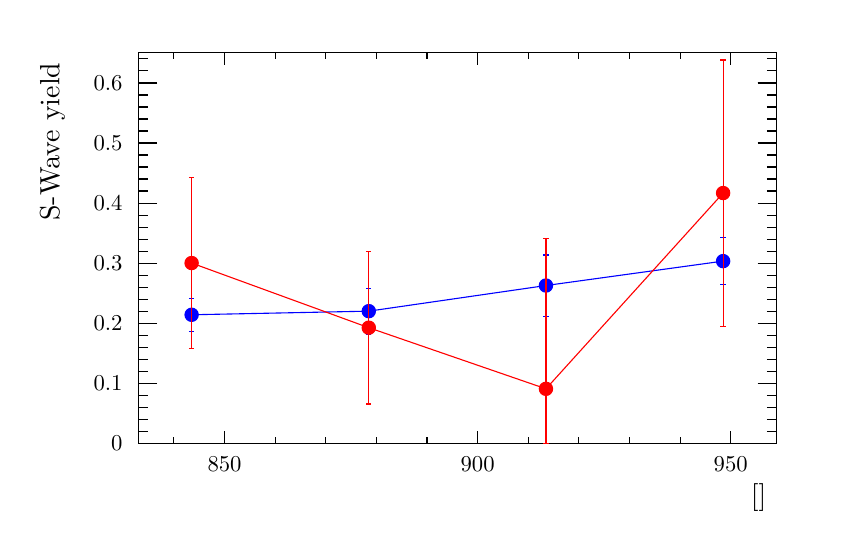
\begin{tikzpicture}
\pgfdeclareplotmark{cross} {
\pgfpathmoveto{\pgfpoint{-0.3\pgfplotmarksize}{\pgfplotmarksize}}
\pgfpathlineto{\pgfpoint{+0.3\pgfplotmarksize}{\pgfplotmarksize}}
\pgfpathlineto{\pgfpoint{+0.3\pgfplotmarksize}{0.3\pgfplotmarksize}}
\pgfpathlineto{\pgfpoint{+1\pgfplotmarksize}{0.3\pgfplotmarksize}}
\pgfpathlineto{\pgfpoint{+1\pgfplotmarksize}{-0.3\pgfplotmarksize}}
\pgfpathlineto{\pgfpoint{+0.3\pgfplotmarksize}{-0.3\pgfplotmarksize}}
\pgfpathlineto{\pgfpoint{+0.3\pgfplotmarksize}{-1.\pgfplotmarksize}}
\pgfpathlineto{\pgfpoint{-0.3\pgfplotmarksize}{-1.\pgfplotmarksize}}
\pgfpathlineto{\pgfpoint{-0.3\pgfplotmarksize}{-0.3\pgfplotmarksize}}
\pgfpathlineto{\pgfpoint{-1.\pgfplotmarksize}{-0.3\pgfplotmarksize}}
\pgfpathlineto{\pgfpoint{-1.\pgfplotmarksize}{0.3\pgfplotmarksize}}
\pgfpathlineto{\pgfpoint{-0.3\pgfplotmarksize}{0.3\pgfplotmarksize}}
\pgfpathclose
\pgfusepathqstroke
}
\pgfdeclareplotmark{cross*} {
\pgfpathmoveto{\pgfpoint{-0.3\pgfplotmarksize}{\pgfplotmarksize}}
\pgfpathlineto{\pgfpoint{+0.3\pgfplotmarksize}{\pgfplotmarksize}}
\pgfpathlineto{\pgfpoint{+0.3\pgfplotmarksize}{0.3\pgfplotmarksize}}
\pgfpathlineto{\pgfpoint{+1\pgfplotmarksize}{0.3\pgfplotmarksize}}
\pgfpathlineto{\pgfpoint{+1\pgfplotmarksize}{-0.3\pgfplotmarksize}}
\pgfpathlineto{\pgfpoint{+0.3\pgfplotmarksize}{-0.3\pgfplotmarksize}}
\pgfpathlineto{\pgfpoint{+0.3\pgfplotmarksize}{-1.\pgfplotmarksize}}
\pgfpathlineto{\pgfpoint{-0.3\pgfplotmarksize}{-1.\pgfplotmarksize}}
\pgfpathlineto{\pgfpoint{-0.3\pgfplotmarksize}{-0.3\pgfplotmarksize}}
\pgfpathlineto{\pgfpoint{-1.\pgfplotmarksize}{-0.3\pgfplotmarksize}}
\pgfpathlineto{\pgfpoint{-1.\pgfplotmarksize}{0.3\pgfplotmarksize}}
\pgfpathlineto{\pgfpoint{-0.3\pgfplotmarksize}{0.3\pgfplotmarksize}}
\pgfpathclose
\pgfusepathqfillstroke
}
\pgfdeclareplotmark{newstar} {
\pgfpathmoveto{\pgfqpoint{0pt}{\pgfplotmarksize}}
\pgfpathlineto{\pgfqpointpolar{44}{0.5\pgfplotmarksize}}
\pgfpathlineto{\pgfqpointpolar{18}{\pgfplotmarksize}}
\pgfpathlineto{\pgfqpointpolar{-20}{0.5\pgfplotmarksize}}
\pgfpathlineto{\pgfqpointpolar{-54}{\pgfplotmarksize}}
\pgfpathlineto{\pgfqpointpolar{-90}{0.5\pgfplotmarksize}}
\pgfpathlineto{\pgfqpointpolar{234}{\pgfplotmarksize}}
\pgfpathlineto{\pgfqpointpolar{198}{0.5\pgfplotmarksize}}
\pgfpathlineto{\pgfqpointpolar{162}{\pgfplotmarksize}}
\pgfpathlineto{\pgfqpointpolar{134}{0.5\pgfplotmarksize}}
\pgfpathclose
\pgfusepathqstroke
}
\pgfdeclareplotmark{newstar*} {
\pgfpathmoveto{\pgfqpoint{0pt}{\pgfplotmarksize}}
\pgfpathlineto{\pgfqpointpolar{44}{0.5\pgfplotmarksize}}
\pgfpathlineto{\pgfqpointpolar{18}{\pgfplotmarksize}}
\pgfpathlineto{\pgfqpointpolar{-20}{0.5\pgfplotmarksize}}
\pgfpathlineto{\pgfqpointpolar{-54}{\pgfplotmarksize}}
\pgfpathlineto{\pgfqpointpolar{-90}{0.5\pgfplotmarksize}}
\pgfpathlineto{\pgfqpointpolar{234}{\pgfplotmarksize}}
\pgfpathlineto{\pgfqpointpolar{198}{0.5\pgfplotmarksize}}
\pgfpathlineto{\pgfqpointpolar{162}{\pgfplotmarksize}}
\pgfpathlineto{\pgfqpointpolar{134}{0.5\pgfplotmarksize}}
\pgfpathclose
\pgfusepathqfillstroke
}
\definecolor{c}{rgb}{1,1,1};
\draw [color=c, fill=c] (0,0) rectangle (10,6.27517);
\draw [color=c, fill=c] (1.4,1.00403) rectangle (9.5,5.96141);
\definecolor{c}{rgb}{0,0,0};
\draw [c] (1.4,1.00403) -- (1.4,5.96141) -- (9.5,5.96141) -- (9.5,1.00403) -- (1.4,1.00403);
\draw [c,line width=0.4] (1.4,1.00403) -- (9.5,1.00403);
\draw [anchor= east] (9.5,0.317272) node[scale=1.00614, rotate=0]{$\mkpi [\mevc]$};
\draw [c,line width=0.4] (2.49286,1.15651) -- (2.49286,1.00403);
\draw [c,line width=0.4] (3.13571,1.08027) -- (3.13571,1.00403);
\draw [c,line width=0.4] (3.77857,1.08027) -- (3.77857,1.00403);
\draw [c,line width=0.4] (4.42143,1.08027) -- (4.42143,1.00403);
\draw [c,line width=0.4] (5.06429,1.08027) -- (5.06429,1.00403);
\draw [c,line width=0.4] (5.70714,1.15651) -- (5.70714,1.00403);
\draw [c,line width=0.4] (6.35,1.08027) -- (6.35,1.00403);
\draw [c,line width=0.4] (6.99286,1.08027) -- (6.99286,1.00403);
\draw [c,line width=0.4] (7.63571,1.08027) -- (7.63571,1.00403);
\draw [c,line width=0.4] (8.27857,1.08027) -- (8.27857,1.00403);
\draw [c,line width=0.4] (8.92143,1.15651) -- (8.92143,1.00403);
\draw [c,line width=0.4] (2.49286,1.15651) -- (2.49286,1.00403);
\draw [c,line width=0.4] (1.85,1.08027) -- (1.85,1.00403);
\draw [c,line width=0.4] (8.92143,1.15651) -- (8.92143,1.00403);
\draw [anchor=base] (2.49286,0.640067) node[scale=0.819821, rotate=0]{850};
\draw [anchor=base] (5.70714,0.640067) node[scale=0.819821, rotate=0]{900};
\draw [anchor=base] (8.92143,0.640067) node[scale=0.819821, rotate=0]{950};
\draw [c,line width=0.4] (1.4,5.96141) -- (9.5,5.96141);
\draw [c,line width=0.4] (2.49286,5.80892) -- (2.49286,5.96141);
\draw [c,line width=0.4] (3.13571,5.88517) -- (3.13571,5.96141);
\draw [c,line width=0.4] (3.77857,5.88517) -- (3.77857,5.96141);
\draw [c,line width=0.4] (4.42143,5.88517) -- (4.42143,5.96141);
\draw [c,line width=0.4] (5.06429,5.88517) -- (5.06429,5.96141);
\draw [c,line width=0.4] (5.70714,5.80892) -- (5.70714,5.96141);
\draw [c,line width=0.4] (6.35,5.88517) -- (6.35,5.96141);
\draw [c,line width=0.4] (6.99286,5.88517) -- (6.99286,5.96141);
\draw [c,line width=0.4] (7.63571,5.88517) -- (7.63571,5.96141);
\draw [c,line width=0.4] (8.27857,5.88517) -- (8.27857,5.96141);
\draw [c,line width=0.4] (8.92143,5.80892) -- (8.92143,5.96141);
\draw [c,line width=0.4] (2.49286,5.80892) -- (2.49286,5.96141);
\draw [c,line width=0.4] (1.85,5.88517) -- (1.85,5.96141);
\draw [c,line width=0.4] (8.92143,5.80892) -- (8.92143,5.96141);
\draw [c,line width=0.4] (1.4,1.00403) -- (1.4,5.96141);
\draw [anchor= east] (0.3056,5.96141) node[scale=1.00614, rotate=90]{S-Wave yield};
\draw [c,line width=0.4] (1.637,1.00403) -- (1.4,1.00403);
\draw [c,line width=0.4] (1.5185,1.15656) -- (1.4,1.15656);
\draw [c,line width=0.4] (1.5185,1.3091) -- (1.4,1.3091);
\draw [c,line width=0.4] (1.5185,1.46163) -- (1.4,1.46163);
\draw [c,line width=0.4] (1.5185,1.61417) -- (1.4,1.61417);
\draw [c,line width=0.4] (1.637,1.7667) -- (1.4,1.7667);
\draw [c,line width=0.4] (1.5185,1.91924) -- (1.4,1.91924);
\draw [c,line width=0.4] (1.5185,2.07177) -- (1.4,2.07177);
\draw [c,line width=0.4] (1.5185,2.22431) -- (1.4,2.22431);
\draw [c,line width=0.4] (1.5185,2.37684) -- (1.4,2.37684);
\draw [c,line width=0.4] (1.637,2.52938) -- (1.4,2.52938);
\draw [c,line width=0.4] (1.5185,2.68191) -- (1.4,2.68191);
\draw [c,line width=0.4] (1.5185,2.83444) -- (1.4,2.83444);
\draw [c,line width=0.4] (1.5185,2.98698) -- (1.4,2.98698);
\draw [c,line width=0.4] (1.5185,3.13951) -- (1.4,3.13951);
\draw [c,line width=0.4] (1.637,3.29205) -- (1.4,3.29205);
\draw [c,line width=0.4] (1.5185,3.44458) -- (1.4,3.44458);
\draw [c,line width=0.4] (1.5185,3.59712) -- (1.4,3.59712);
\draw [c,line width=0.4] (1.5185,3.74965) -- (1.4,3.74965);
\draw [c,line width=0.4] (1.5185,3.90219) -- (1.4,3.90219);
\draw [c,line width=0.4] (1.637,4.05472) -- (1.4,4.05472);
\draw [c,line width=0.4] (1.5185,4.20726) -- (1.4,4.20726);
\draw [c,line width=0.4] (1.5185,4.35979) -- (1.4,4.35979);
\draw [c,line width=0.4] (1.5185,4.51233) -- (1.4,4.51233);
\draw [c,line width=0.4] (1.5185,4.66486) -- (1.4,4.66486);
\draw [c,line width=0.4] (1.637,4.8174) -- (1.4,4.8174);
\draw [c,line width=0.4] (1.5185,4.96993) -- (1.4,4.96993);
\draw [c,line width=0.4] (1.5185,5.12247) -- (1.4,5.12247);
\draw [c,line width=0.4] (1.5185,5.275) -- (1.4,5.275);
\draw [c,line width=0.4] (1.5185,5.42754) -- (1.4,5.42754);
\draw [c,line width=0.4] (1.637,5.58007) -- (1.4,5.58007);
\draw [c,line width=0.4] (1.637,5.58007) -- (1.4,5.58007);
\draw [c,line width=0.4] (1.5185,5.73261) -- (1.4,5.73261);
\draw [c,line width=0.4] (1.5185,5.88514) -- (1.4,5.88514);
\draw [anchor= east] (1.3,1.00403) node[scale=0.819821, rotate=0]{0};
\draw [anchor= east] (1.3,1.7667) node[scale=0.819821, rotate=0]{0.1};
\draw [anchor= east] (1.3,2.52938) node[scale=0.819821, rotate=0]{0.2};
\draw [anchor= east] (1.3,3.29205) node[scale=0.819821, rotate=0]{0.3};
\draw [anchor= east] (1.3,4.05472) node[scale=0.819821, rotate=0]{0.4};
\draw [anchor= east] (1.3,4.8174) node[scale=0.819821, rotate=0]{0.5};
\draw [anchor= east] (1.3,5.58007) node[scale=0.819821, rotate=0]{0.6};
\draw [c,line width=0.4] (9.5,1.00403) -- (9.5,5.96141);
\draw [c,line width=0.4] (9.263,1.00403) -- (9.5,1.00403);
\draw [c,line width=0.4] (9.3815,1.15656) -- (9.5,1.15656);
\draw [c,line width=0.4] (9.3815,1.3091) -- (9.5,1.3091);
\draw [c,line width=0.4] (9.3815,1.46163) -- (9.5,1.46163);
\draw [c,line width=0.4] (9.3815,1.61417) -- (9.5,1.61417);
\draw [c,line width=0.4] (9.263,1.7667) -- (9.5,1.7667);
\draw [c,line width=0.4] (9.3815,1.91924) -- (9.5,1.91924);
\draw [c,line width=0.4] (9.3815,2.07177) -- (9.5,2.07177);
\draw [c,line width=0.4] (9.3815,2.22431) -- (9.5,2.22431);
\draw [c,line width=0.4] (9.3815,2.37684) -- (9.5,2.37684);
\draw [c,line width=0.4] (9.263,2.52938) -- (9.5,2.52938);
\draw [c,line width=0.4] (9.3815,2.68191) -- (9.5,2.68191);
\draw [c,line width=0.4] (9.3815,2.83444) -- (9.5,2.83444);
\draw [c,line width=0.4] (9.3815,2.98698) -- (9.5,2.98698);
\draw [c,line width=0.4] (9.3815,3.13951) -- (9.5,3.13951);
\draw [c,line width=0.4] (9.263,3.29205) -- (9.5,3.29205);
\draw [c,line width=0.4] (9.3815,3.44458) -- (9.5,3.44458);
\draw [c,line width=0.4] (9.3815,3.59712) -- (9.5,3.59712);
\draw [c,line width=0.4] (9.3815,3.74965) -- (9.5,3.74965);
\draw [c,line width=0.4] (9.3815,3.90219) -- (9.5,3.90219);
\draw [c,line width=0.4] (9.263,4.05472) -- (9.5,4.05472);
\draw [c,line width=0.4] (9.3815,4.20726) -- (9.5,4.20726);
\draw [c,line width=0.4] (9.3815,4.35979) -- (9.5,4.35979);
\draw [c,line width=0.4] (9.3815,4.51233) -- (9.5,4.51233);
\draw [c,line width=0.4] (9.3815,4.66486) -- (9.5,4.66486);
\draw [c,line width=0.4] (9.263,4.8174) -- (9.5,4.8174);
\draw [c,line width=0.4] (9.3815,4.96993) -- (9.5,4.96993);
\draw [c,line width=0.4] (9.3815,5.12247) -- (9.5,5.12247);
\draw [c,line width=0.4] (9.3815,5.275) -- (9.5,5.275);
\draw [c,line width=0.4] (9.3815,5.42754) -- (9.5,5.42754);
\draw [c,line width=0.4] (9.263,5.58007) -- (9.5,5.58007);
\draw [c,line width=0.4] (9.263,5.58007) -- (9.5,5.58007);
\draw [c,line width=0.4] (9.3815,5.73261) -- (9.5,5.73261);
\draw [c,line width=0.4] (9.3815,5.88514) -- (9.5,5.88514);
\definecolor{c}{rgb}{0,0,1};
\draw [c,line width=0.4] (2.075,2.63604) -- (4.325,2.68193) -- (6.575,3.00741) -- (8.825,3.31747);
\foreach \P in {(2.075,2.63604),(4.325,2.68193),(6.575,3.00741),(8.825,3.31747)}{\draw[mark options={color=c,fill=c},mark size=2.402402pt,mark=*] plot coordinates {\P};}
\draw [c,line width=0.4] (2.075,2.70315) -- (2.075,2.84806);
\draw [c,line width=0.4] (2.04144,2.84806) -- (2.10856,2.84806);
\draw [c,line width=0.4] (2.075,2.56892) -- (2.075,2.42402);
\draw [c,line width=0.4] (2.04144,2.42402) -- (2.10856,2.42402);
\draw [c,line width=0.4] (4.325,2.74904) -- (4.325,2.97344);
\draw [c,line width=0.4] (4.29144,2.97344) -- (4.35856,2.97344);
\draw [c,line width=0.4] (4.325,2.61481) -- (4.325,2.39042);
\draw [c,line width=0.4] (4.29144,2.39042) -- (4.35856,2.39042);
\draw [c,line width=0.4] (6.575,3.07452) -- (6.575,3.39535);
\draw [c,line width=0.4] (6.54144,3.39535) -- (6.60856,3.39535);
\draw [c,line width=0.4] (6.575,2.94029) -- (6.575,2.61946);
\draw [c,line width=0.4] (6.54144,2.61946) -- (6.60856,2.61946);
\draw [c,line width=0.4] (8.825,3.38459) -- (8.825,3.61574);
\draw [c,line width=0.4] (8.79144,3.61574) -- (8.85856,3.61574);
\draw [c,line width=0.4] (8.825,3.25036) -- (8.825,3.01921);
\draw [c,line width=0.4] (8.79144,3.01921) -- (8.85856,3.01921);
\definecolor{c}{rgb}{1,0,0};
\draw [c,line width=0.4] (2.075,3.36015) -- (2.075,4.38263);
\draw [c,line width=0.4] (2.04144,4.38263) -- (2.10856,4.38263);
\draw [c,line width=0.4] (2.075,3.22592) -- (2.075,2.20343);
\draw [c,line width=0.4] (2.04144,2.20343) -- (2.10856,2.20343);
\draw [c,line width=0.4] (4.325,2.53912) -- (4.325,3.44049);
\draw [c,line width=0.4] (4.29144,3.44049) -- (4.35856,3.44049);
\draw [c,line width=0.4] (4.325,2.4049) -- (4.325,1.50353);
\draw [c,line width=0.4] (4.29144,1.50353) -- (4.35856,1.50353);
\draw [c,line width=0.4] (6.575,1.76295) -- (6.575,3.60437);
\draw [c,line width=0.4] (6.54144,3.60437) -- (6.60856,3.60437);
\draw [c,line width=0.4] (6.575,1.62872) -- (6.575,1.00403);
\draw [c,line width=0.4] (6.54144,1.00403) -- (6.60856,1.00403);
\draw [c,line width=0.4] (8.825,4.24909) -- (8.825,5.87178);
\draw [c,line width=0.4] (8.79144,5.87178) -- (8.85856,5.87178);
\draw [c,line width=0.4] (8.825,4.11486) -- (8.825,2.49217);
\draw [c,line width=0.4] (8.79144,2.49217) -- (8.85856,2.49217);
\draw [c,line width=0.4] (2.075,3.29303) -- (4.325,2.47201) -- (6.575,1.69583) -- (8.825,4.18197);
\foreach \P in {(2.075,3.29303),(4.325,2.47201),(6.575,1.69583),(8.825,4.18197)}{\draw[mark options={color=c,fill=c},mark size=2.402402pt,mark=*] plot coordinates {\P};}
\end{tikzpicture}
}
%%     \caption{}
%%     \label{opasd}
%%   \end{subfigure}
%%   \begin{subfigure}{0.5\textwidth}
%%     \tikzsetnextfilename{phasesoffset_} 
%%     \scalebox{0.60}{\begin{tikzpicture}
\pgfdeclareplotmark{cross} {
\pgfpathmoveto{\pgfpoint{-0.3\pgfplotmarksize}{\pgfplotmarksize}}
\pgfpathlineto{\pgfpoint{+0.3\pgfplotmarksize}{\pgfplotmarksize}}
\pgfpathlineto{\pgfpoint{+0.3\pgfplotmarksize}{0.3\pgfplotmarksize}}
\pgfpathlineto{\pgfpoint{+1\pgfplotmarksize}{0.3\pgfplotmarksize}}
\pgfpathlineto{\pgfpoint{+1\pgfplotmarksize}{-0.3\pgfplotmarksize}}
\pgfpathlineto{\pgfpoint{+0.3\pgfplotmarksize}{-0.3\pgfplotmarksize}}
\pgfpathlineto{\pgfpoint{+0.3\pgfplotmarksize}{-1.\pgfplotmarksize}}
\pgfpathlineto{\pgfpoint{-0.3\pgfplotmarksize}{-1.\pgfplotmarksize}}
\pgfpathlineto{\pgfpoint{-0.3\pgfplotmarksize}{-0.3\pgfplotmarksize}}
\pgfpathlineto{\pgfpoint{-1.\pgfplotmarksize}{-0.3\pgfplotmarksize}}
\pgfpathlineto{\pgfpoint{-1.\pgfplotmarksize}{0.3\pgfplotmarksize}}
\pgfpathlineto{\pgfpoint{-0.3\pgfplotmarksize}{0.3\pgfplotmarksize}}
\pgfpathclose
\pgfusepathqstroke
}
\pgfdeclareplotmark{cross*} {
\pgfpathmoveto{\pgfpoint{-0.3\pgfplotmarksize}{\pgfplotmarksize}}
\pgfpathlineto{\pgfpoint{+0.3\pgfplotmarksize}{\pgfplotmarksize}}
\pgfpathlineto{\pgfpoint{+0.3\pgfplotmarksize}{0.3\pgfplotmarksize}}
\pgfpathlineto{\pgfpoint{+1\pgfplotmarksize}{0.3\pgfplotmarksize}}
\pgfpathlineto{\pgfpoint{+1\pgfplotmarksize}{-0.3\pgfplotmarksize}}
\pgfpathlineto{\pgfpoint{+0.3\pgfplotmarksize}{-0.3\pgfplotmarksize}}
\pgfpathlineto{\pgfpoint{+0.3\pgfplotmarksize}{-1.\pgfplotmarksize}}
\pgfpathlineto{\pgfpoint{-0.3\pgfplotmarksize}{-1.\pgfplotmarksize}}
\pgfpathlineto{\pgfpoint{-0.3\pgfplotmarksize}{-0.3\pgfplotmarksize}}
\pgfpathlineto{\pgfpoint{-1.\pgfplotmarksize}{-0.3\pgfplotmarksize}}
\pgfpathlineto{\pgfpoint{-1.\pgfplotmarksize}{0.3\pgfplotmarksize}}
\pgfpathlineto{\pgfpoint{-0.3\pgfplotmarksize}{0.3\pgfplotmarksize}}
\pgfpathclose
\pgfusepathqfillstroke
}
\pgfdeclareplotmark{newstar} {
\pgfpathmoveto{\pgfqpoint{0pt}{\pgfplotmarksize}}
\pgfpathlineto{\pgfqpointpolar{44}{0.5\pgfplotmarksize}}
\pgfpathlineto{\pgfqpointpolar{18}{\pgfplotmarksize}}
\pgfpathlineto{\pgfqpointpolar{-20}{0.5\pgfplotmarksize}}
\pgfpathlineto{\pgfqpointpolar{-54}{\pgfplotmarksize}}
\pgfpathlineto{\pgfqpointpolar{-90}{0.5\pgfplotmarksize}}
\pgfpathlineto{\pgfqpointpolar{234}{\pgfplotmarksize}}
\pgfpathlineto{\pgfqpointpolar{198}{0.5\pgfplotmarksize}}
\pgfpathlineto{\pgfqpointpolar{162}{\pgfplotmarksize}}
\pgfpathlineto{\pgfqpointpolar{134}{0.5\pgfplotmarksize}}
\pgfpathclose
\pgfusepathqstroke
}
\pgfdeclareplotmark{newstar*} {
\pgfpathmoveto{\pgfqpoint{0pt}{\pgfplotmarksize}}
\pgfpathlineto{\pgfqpointpolar{44}{0.5\pgfplotmarksize}}
\pgfpathlineto{\pgfqpointpolar{18}{\pgfplotmarksize}}
\pgfpathlineto{\pgfqpointpolar{-20}{0.5\pgfplotmarksize}}
\pgfpathlineto{\pgfqpointpolar{-54}{\pgfplotmarksize}}
\pgfpathlineto{\pgfqpointpolar{-90}{0.5\pgfplotmarksize}}
\pgfpathlineto{\pgfqpointpolar{234}{\pgfplotmarksize}}
\pgfpathlineto{\pgfqpointpolar{198}{0.5\pgfplotmarksize}}
\pgfpathlineto{\pgfqpointpolar{162}{\pgfplotmarksize}}
\pgfpathlineto{\pgfqpointpolar{134}{0.5\pgfplotmarksize}}
\pgfpathclose
\pgfusepathqfillstroke
}
\definecolor{c}{rgb}{1,1,1};
\draw [color=c, fill=c] (0,0) rectangle (10,6.27517);
\draw [color=c, fill=c] (1.4,1.00403) rectangle (9.5,5.96141);
\definecolor{c}{rgb}{0,0,0};
\draw [c] (1.4,1.00403) -- (1.4,5.96141) -- (9.5,5.96141) -- (9.5,1.00403) -- (1.4,1.00403);
\draw [c,line width=0.4] (1.4,1.00403) -- (9.5,1.00403);
\draw [anchor= east] (9.5,0.317272) node[scale=1.00614, rotate=0]{$\mkpi [\mevc]$};
\draw [c,line width=0.4] (2.49286,1.15651) -- (2.49286,1.00403);
\draw [c,line width=0.4] (3.13571,1.08027) -- (3.13571,1.00403);
\draw [c,line width=0.4] (3.77857,1.08027) -- (3.77857,1.00403);
\draw [c,line width=0.4] (4.42143,1.08027) -- (4.42143,1.00403);
\draw [c,line width=0.4] (5.06429,1.08027) -- (5.06429,1.00403);
\draw [c,line width=0.4] (5.70714,1.15651) -- (5.70714,1.00403);
\draw [c,line width=0.4] (6.35,1.08027) -- (6.35,1.00403);
\draw [c,line width=0.4] (6.99286,1.08027) -- (6.99286,1.00403);
\draw [c,line width=0.4] (7.63571,1.08027) -- (7.63571,1.00403);
\draw [c,line width=0.4] (8.27857,1.08027) -- (8.27857,1.00403);
\draw [c,line width=0.4] (8.92143,1.15651) -- (8.92143,1.00403);
\draw [c,line width=0.4] (2.49286,1.15651) -- (2.49286,1.00403);
\draw [c,line width=0.4] (1.85,1.08027) -- (1.85,1.00403);
\draw [c,line width=0.4] (8.92143,1.15651) -- (8.92143,1.00403);
\draw [anchor=base] (2.49286,0.640067) node[scale=0.819821, rotate=0]{850};
\draw [anchor=base] (5.70714,0.640067) node[scale=0.819821, rotate=0]{900};
\draw [anchor=base] (8.92143,0.640067) node[scale=0.819821, rotate=0]{950};
\draw [c,line width=0.4] (1.4,5.96141) -- (9.5,5.96141);
\draw [c,line width=0.4] (2.49286,5.80892) -- (2.49286,5.96141);
\draw [c,line width=0.4] (3.13571,5.88517) -- (3.13571,5.96141);
\draw [c,line width=0.4] (3.77857,5.88517) -- (3.77857,5.96141);
\draw [c,line width=0.4] (4.42143,5.88517) -- (4.42143,5.96141);
\draw [c,line width=0.4] (5.06429,5.88517) -- (5.06429,5.96141);
\draw [c,line width=0.4] (5.70714,5.80892) -- (5.70714,5.96141);
\draw [c,line width=0.4] (6.35,5.88517) -- (6.35,5.96141);
\draw [c,line width=0.4] (6.99286,5.88517) -- (6.99286,5.96141);
\draw [c,line width=0.4] (7.63571,5.88517) -- (7.63571,5.96141);
\draw [c,line width=0.4] (8.27857,5.88517) -- (8.27857,5.96141);
\draw [c,line width=0.4] (8.92143,5.80892) -- (8.92143,5.96141);
\draw [c,line width=0.4] (2.49286,5.80892) -- (2.49286,5.96141);
\draw [c,line width=0.4] (1.85,5.88517) -- (1.85,5.96141);
\draw [c,line width=0.4] (8.92143,5.80892) -- (8.92143,5.96141);
\draw [c,line width=0.4] (1.4,1.00403) -- (1.4,5.96141);
\draw [anchor= east] (0.3056,5.96141) node[scale=1.00614, rotate=90]{$\color{red}{\deltaS{\Bs}} , \color{blue}{\deltaS{\Bd}}$};
\draw [c,line width=0.4] (1.637,1.00403) -- (1.4,1.00403);
\draw [c,line width=0.4] (1.5185,1.12796) -- (1.4,1.12796);
\draw [c,line width=0.4] (1.5185,1.2519) -- (1.4,1.2519);
\draw [c,line width=0.4] (1.5185,1.37583) -- (1.4,1.37583);
\draw [c,line width=0.4] (1.5185,1.49977) -- (1.4,1.49977);
\draw [c,line width=0.4] (1.637,1.6237) -- (1.4,1.6237);
\draw [c,line width=0.4] (1.5185,1.74763) -- (1.4,1.74763);
\draw [c,line width=0.4] (1.5185,1.87157) -- (1.4,1.87157);
\draw [c,line width=0.4] (1.5185,1.9955) -- (1.4,1.9955);
\draw [c,line width=0.4] (1.5185,2.11944) -- (1.4,2.11944);
\draw [c,line width=0.4] (1.637,2.24337) -- (1.4,2.24337);
\draw [c,line width=0.4] (1.5185,2.36731) -- (1.4,2.36731);
\draw [c,line width=0.4] (1.5185,2.49124) -- (1.4,2.49124);
\draw [c,line width=0.4] (1.5185,2.61518) -- (1.4,2.61518);
\draw [c,line width=0.4] (1.5185,2.73911) -- (1.4,2.73911);
\draw [c,line width=0.4] (1.637,2.86305) -- (1.4,2.86305);
\draw [c,line width=0.4] (1.5185,2.98698) -- (1.4,2.98698);
\draw [c,line width=0.4] (1.5185,3.11091) -- (1.4,3.11091);
\draw [c,line width=0.4] (1.5185,3.23485) -- (1.4,3.23485);
\draw [c,line width=0.4] (1.5185,3.35878) -- (1.4,3.35878);
\draw [c,line width=0.4] (1.637,3.48272) -- (1.4,3.48272);
\draw [c,line width=0.4] (1.5185,3.60665) -- (1.4,3.60665);
\draw [c,line width=0.4] (1.5185,3.73059) -- (1.4,3.73059);
\draw [c,line width=0.4] (1.5185,3.85452) -- (1.4,3.85452);
\draw [c,line width=0.4] (1.5185,3.97846) -- (1.4,3.97846);
\draw [c,line width=0.4] (1.637,4.10239) -- (1.4,4.10239);
\draw [c,line width=0.4] (1.5185,4.22633) -- (1.4,4.22633);
\draw [c,line width=0.4] (1.5185,4.35026) -- (1.4,4.35026);
\draw [c,line width=0.4] (1.5185,4.47419) -- (1.4,4.47419);
\draw [c,line width=0.4] (1.5185,4.59813) -- (1.4,4.59813);
\draw [c,line width=0.4] (1.637,4.72206) -- (1.4,4.72206);
\draw [c,line width=0.4] (1.5185,4.846) -- (1.4,4.846);
\draw [c,line width=0.4] (1.5185,4.96993) -- (1.4,4.96993);
\draw [c,line width=0.4] (1.5185,5.09387) -- (1.4,5.09387);
\draw [c,line width=0.4] (1.5185,5.2178) -- (1.4,5.2178);
\draw [c,line width=0.4] (1.637,5.34174) -- (1.4,5.34174);
\draw [c,line width=0.4] (1.5185,5.46567) -- (1.4,5.46567);
\draw [c,line width=0.4] (1.5185,5.58961) -- (1.4,5.58961);
\draw [c,line width=0.4] (1.5185,5.71354) -- (1.4,5.71354);
\draw [c,line width=0.4] (1.5185,5.83747) -- (1.4,5.83747);
\draw [c,line width=0.4] (1.637,5.96141) -- (1.4,5.96141);
\draw [anchor= east] (1.3,1.00403) node[scale=0.819821, rotate=0]{-4};
\draw [anchor= east] (1.3,1.6237) node[scale=0.819821, rotate=0]{-3};
\draw [anchor= east] (1.3,2.24337) node[scale=0.819821, rotate=0]{-2};
\draw [anchor= east] (1.3,2.86305) node[scale=0.819821, rotate=0]{-1};
\draw [anchor= east] (1.3,3.48272) node[scale=0.819821, rotate=0]{0};
\draw [anchor= east] (1.3,4.10239) node[scale=0.819821, rotate=0]{1};
\draw [anchor= east] (1.3,4.72206) node[scale=0.819821, rotate=0]{2};
\draw [anchor= east] (1.3,5.34174) node[scale=0.819821, rotate=0]{3};
\draw [anchor= east] (1.3,5.96141) node[scale=0.819821, rotate=0]{4};
\draw [c,line width=0.4] (9.5,1.00403) -- (9.5,5.96141);
\draw [c,line width=0.4] (9.263,1.00403) -- (9.5,1.00403);
\draw [c,line width=0.4] (9.3815,1.12796) -- (9.5,1.12796);
\draw [c,line width=0.4] (9.3815,1.2519) -- (9.5,1.2519);
\draw [c,line width=0.4] (9.3815,1.37583) -- (9.5,1.37583);
\draw [c,line width=0.4] (9.3815,1.49977) -- (9.5,1.49977);
\draw [c,line width=0.4] (9.263,1.6237) -- (9.5,1.6237);
\draw [c,line width=0.4] (9.3815,1.74763) -- (9.5,1.74763);
\draw [c,line width=0.4] (9.3815,1.87157) -- (9.5,1.87157);
\draw [c,line width=0.4] (9.3815,1.9955) -- (9.5,1.9955);
\draw [c,line width=0.4] (9.3815,2.11944) -- (9.5,2.11944);
\draw [c,line width=0.4] (9.263,2.24337) -- (9.5,2.24337);
\draw [c,line width=0.4] (9.3815,2.36731) -- (9.5,2.36731);
\draw [c,line width=0.4] (9.3815,2.49124) -- (9.5,2.49124);
\draw [c,line width=0.4] (9.3815,2.61518) -- (9.5,2.61518);
\draw [c,line width=0.4] (9.3815,2.73911) -- (9.5,2.73911);
\draw [c,line width=0.4] (9.263,2.86305) -- (9.5,2.86305);
\draw [c,line width=0.4] (9.3815,2.98698) -- (9.5,2.98698);
\draw [c,line width=0.4] (9.3815,3.11091) -- (9.5,3.11091);
\draw [c,line width=0.4] (9.3815,3.23485) -- (9.5,3.23485);
\draw [c,line width=0.4] (9.3815,3.35878) -- (9.5,3.35878);
\draw [c,line width=0.4] (9.263,3.48272) -- (9.5,3.48272);
\draw [c,line width=0.4] (9.3815,3.60665) -- (9.5,3.60665);
\draw [c,line width=0.4] (9.3815,3.73059) -- (9.5,3.73059);
\draw [c,line width=0.4] (9.3815,3.85452) -- (9.5,3.85452);
\draw [c,line width=0.4] (9.3815,3.97846) -- (9.5,3.97846);
\draw [c,line width=0.4] (9.263,4.10239) -- (9.5,4.10239);
\draw [c,line width=0.4] (9.3815,4.22633) -- (9.5,4.22633);
\draw [c,line width=0.4] (9.3815,4.35026) -- (9.5,4.35026);
\draw [c,line width=0.4] (9.3815,4.47419) -- (9.5,4.47419);
\draw [c,line width=0.4] (9.3815,4.59813) -- (9.5,4.59813);
\draw [c,line width=0.4] (9.263,4.72206) -- (9.5,4.72206);
\draw [c,line width=0.4] (9.3815,4.846) -- (9.5,4.846);
\draw [c,line width=0.4] (9.3815,4.96993) -- (9.5,4.96993);
\draw [c,line width=0.4] (9.3815,5.09387) -- (9.5,5.09387);
\draw [c,line width=0.4] (9.3815,5.2178) -- (9.5,5.2178);
\draw [c,line width=0.4] (9.263,5.34174) -- (9.5,5.34174);
\draw [c,line width=0.4] (9.3815,5.46567) -- (9.5,5.46567);
\draw [c,line width=0.4] (9.3815,5.58961) -- (9.5,5.58961);
\draw [c,line width=0.4] (9.3815,5.71354) -- (9.5,5.71354);
\draw [c,line width=0.4] (9.3815,5.83747) -- (9.5,5.83747);
\draw [c,line width=0.4] (9.263,5.96141) -- (9.5,5.96141);
\definecolor{c}{rgb}{1,0,0};
\draw [c,line width=0.4] (2.075,3.48272) -- (4.325,2.91882) -- (6.575,2.41068) -- (8.825,2.16281);
\foreach \P in {(2.075,3.48272),(4.325,2.91882),(6.575,2.41068),(8.825,2.16281)}{\draw[mark options={color=c,fill=c},mark size=2.402402pt,mark=*] plot coordinates {\P};}
\draw [c,line width=0.4] (2.075,3.54983) -- (2.075,3.57567);
\draw [c,line width=0.4] (2.04144,3.57567) -- (2.10856,3.57567);
\draw [c,line width=0.4] (2.075,3.4156) -- (2.075,3.38977);
\draw [c,line width=0.4] (2.04144,3.38977) -- (2.10856,3.38977);
\draw [c,line width=0.4] (4.325,2.98593) -- (4.325,3.05514);
\draw [c,line width=0.4] (4.29144,3.05514) -- (4.35856,3.05514);
\draw [c,line width=0.4] (4.325,2.8517) -- (4.325,2.78249);
\draw [c,line width=0.4] (4.29144,2.78249) -- (4.35856,2.78249);
\draw [c,line width=0.4] (6.575,2.4778) -- (6.575,2.55941);
\draw [c,line width=0.4] (6.54144,2.55941) -- (6.60856,2.55941);
\draw [c,line width=0.4] (6.575,2.34357) -- (6.575,2.26196);
\draw [c,line width=0.4] (6.54144,2.26196) -- (6.60856,2.26196);
\draw [c,line width=0.4] (8.825,2.22993) -- (8.825,2.23718);
\draw [c,line width=0.4] (8.79144,2.23718) -- (8.85856,2.23718);
\draw [c,line width=0.4] (8.825,2.0957) -- (8.825,2.08845);
\draw [c,line width=0.4] (8.79144,2.08845) -- (8.85856,2.08845);
\definecolor{c}{rgb}{0,0,1};
\draw [c,line width=0.4] (2.075,3.48272) -- (4.325,3.09232) -- (6.575,2.5718) -- (8.825,2.36731);
\foreach \P in {(2.075,3.48272),(4.325,3.09232),(6.575,2.5718),(8.825,2.36731)}{\draw[mark options={color=c,fill=c},mark size=2.402402pt,mark=*] plot coordinates {\P};}
\end{tikzpicture}
}
%%     \caption{}
%%     \label{opa}
%%   \end{subfigure}%
%% \caption{\pwave and \swave trends of \BsJpsiKst \BdJpsiKst fractions and phases}
%% \end{figure}

%%%%%%%%%%%%%%%%%%%%%%%%%%%%%%%%%%%%%%%%%%%%%%%%%%%
\subsection{Systematic Uncertainties}
\label{systemics}
%%%%%%%%%%%%%%%%%%%%%%%%%%%%%%%%%%%%%%%%%%%%%%%%%%%
The different source of systematic uncertainties on the \Bs angular parameters, as well as on the branching fraction
are pesented int he curent section.

\subsubsection{Angular acceptance}
\label{systAngAcc}
The efficiency moments as described in \secref{Accceptance} are computed with a limited size simulation sample
and are thus their central values are subected to statistical fluctuations. To account for this limitation the
efficiency moments are allowed to float in the angular fit to the data with a multivariant gaussian constrain within $5$
standard deviations from their nominal value. The multivariant gaussian takes properly into acount their correlations.
In addition this systematic covers any potential difference in the acceptance between data and simulated sample
that has not been corrected by the iterative procedure described in \secref{Accceptance_Corrections}. Furthermore,
the constrain of \equref{eff_func_constr} used to force the acceptance positive assumes that the acceptance is zero
at $\cos\thetaK=1$ for any value of $(\cos\thetamu,\phihel)$. This assumption might not be exactly true. It could be
that the value of the acceptance at that point is very small but not zero. This systematic effect is accounted for
by adding a term\footnote{with the appropriate $\frac{1}{2\sqrt{\pi}}$ normalization} to \equref{eff_func_final} and allowing it to 
float in the above mentioned fit to the data. The differences in the prameters of intereset between the best fit 
of \tabref{bestFitResult} and the fit with the floating acceptanceis taken as a systematic uncertainty. 

\begin{table}[!h]
  \center
  \begin{tabular}{c c c c c c }
    \hline
                             & $\Acp{0}$  &  $\Acp{\parallel}$ &  $\Acp{\perp}$ & $\Acp{S}$ \\
    \hline
    Mass parameters and \Bd contamination & $            0.001$ & $            0.001$ & $                -$ & $            0.001$ \\ 
    \dwave contribution                   & $            0.002$ & $            0.015$ & $            0.002$ & $                -$ \\ 
    Mass---$\cos\thetamu$ correlations    & $            0.014$ & $^{+0.009}_{-0.012}$ & $            0.016$ & $^{+0.023}_{-0.029}$      \\
    Angular acceptance                    & $            0.003$ & $            0.003$ & $            0.002$ & $            0.001$ \\
    Peaking background                    & $^{+0.003}_{-0.004}$   & $^{+0.012}_{-0.004}$ & $            0.002$ & $            0.001$    \\
    $C_{SP}$ factors                       & $            0.001$ & $            0.002$ & $            0.002$ & $                -$ \\
    Fit bias                              & $            0.009$ & $            0.007$ & $            0.011$ & $            0.037$ \\
    \hline                                                                                                                          
    Total uncertainties                   & $^{+0.27}_{-0.28}$ & $            0.14$ & $^{+0.20}_{-0.21}$ & $^{+0.45}_{-0.48}$         \\
    \hline
  \end{tabular}
  \caption{\small Best fit values of the parameters of intereset.}
  \label{systematics_acp}
\end{table}

\subsubsection{$m(\Jpsi K^+\pi^-)$ mass model}
\label{systMassModel}
Not all the PDF parameters are free to vary in the mass fit to the data as described in \secref{Event_Selection}. 
These parameters are fixed to values taken from simulated events. 
In order to account for systematic uncertainties due to these fixed parameters, the mass fit is repeated 1000 times. In each fit
to the data the values of those fixed parameters are taken from a Gaussian distribution. The mean and width of the gaussian are
taken from a mass fit to the simulated data (this last fit is the one that those fixed parameters were estimated in the first palce.)
Correlations among those parameters are taken into account in this procedure. Lastly, for each one of the 1000 different mass fits
a new sets of \sWeights is computed and subsequently the angular fit is performed. The result is one gausian like distribution
for each of the angular parameters of interest. The one standard deviation interval of this distribution is assigned as a systematic to that paramter.

In addition, another systematic to account for event leakage from the $\Bd$ to the $\Bs$ peak is assigned. As mentioned in \secref{Event_Selection}
$\alpha$ is the parameter cotroling the tails of the mass peak and it is fixed during the mass fit to the data. Complementary to the treatment of 
the fixed paramters in the above paragraph, the paramter $\alpha$ of the $\Bd$ peak is further scrutinesd. Particularly the mass fit to the data
is repeated with $\alpha$ set to infinity and $\alpha$ floating. The first case, according to the Hypatia function, implies that any contribution
to the tails other than resolution is ignored. Those two mass fits yield two more set of \sWeights and two more angular fits. The difference in 
the value of the fitted angular paramters between those two case is assigned as a systematic.{{red} Confrim this with Simon. ANA note is not clear enough.}

\begin{table}[!h]
  \center
  \begin{tabular}{c c c c c c }
    \hline
                 & $\fP{0}$ & $\fP{\parallel}$ & $\ampPhase{\parallel}$ & $\ampPhase{\perp}$  \\                          
    \hline
    Mass parameters and \Bd contamination &   $                 -$ & $                 -$ & $                 -$ & $                 -$ \\
    \dwave contribution                   &   $             0.004$ & $             0.003$ & $                 -$ & $                 -$ \\
    Mass---$\cos\thetamu$ correlations    &   $             0.007$ & $             0.006$ & $             0.070$ & $^{+0.020}_{-0.040}$     \\
    Angular acceptance                    &   $             0.003$ & $             0.001$ & $             0.002$ & $             0.001$ \\
    Peaking background                    &   $^{+0.004}_{-0.003}$    & $             0.002$ & $             0.020$ & $             0.010$    \\
    $C_{SP}$ factors                       &  $                 -$  & $             0.001$ & $                 -$ & $                 -$  \\
    Fit bias                              &   $                 -$ & $                 -$ & $             0.004$ & $             0.018$ \\
    \hline                                                                                                                             
    Total uncertainties                   &   $^{+0.40}_{-0.37}$ & $^{+0.26}_{-0.27}$ & $^{+0.45}_{-0.44}$ & $^{+0.26}_{-0.39}$                     \\
    \hline
  \end{tabular}
  \caption{\small Best fit values of the parameters of intereset.}
  \label{systematics_pwave}
\end{table}

\subsubsection{Peaking backgrounds}
\label{systPeakBkg}
Peaking backgound estiamtes have an inpact on the mass fit and eventually on the computed set of \sWeights.
Those estimates are summarized in \tabref{peaking_bkg_yields}, where one can see that they come with a statisitcal uncertainty as well.
To account for tha last uncertainty  the estimates of all peaking backgorund species (\BsJpsiKK, \BsJpsipipi, \BdJpsipipi, and \LbJpsipK)
are swifted one at a time by 1 standard deviation. The result is a different set of \sWeights for each specie.
Susequenlty the angular fit is performed with that set of \sWeights. The difference in the angular parameters
between the last fit and the nominal angular fit is taken as a systematic uncertainty for the particular peaking background specie.
Individual contributions from all species to a certaina gular paramter are added in quadrature and assigned as a systematic.

\subsubsection{Correlations between mass and angles in the \sPlot context}
\label{systCorrs}
Correlations between the $\Bs$ invariant mass and the $\cos\thetamu$ angular distribution is taken into account
by performing the mass fit in 5 bins of $\cos\thetamu$. Since the choice of 5 bins is arbitrary the mass fit is
repeated in 3 and 6 $\cos\thetamu$ bins as well. The result is two more sets of sWeights. For each set the angular
fit is performed and the differences in each of the paramters of intereset are added in quadratures. The last quadratic
sum is assigned as systematic. 

\subsubsection{Fit bias}
\label{systFitBias}
Potenntial fit biases of the fitting procedure are addressed in \secref{Toy_Experiments_Study} and the corresponding 
results are reported in \tabref{pull_table}. The reported biases on the parameters of itnereset are assigned as a systematic uncertainty.

\begin{table}[!h]
  \center
  \begin{tabular}{c c c c c c }
    \hline
                 & $\fS{1}$ & $\fS{2}$ & $\fS{3}$ & $\fS{4}$  \\                          
    \hline
    Mass parameters and \Bd contamination &  $             0.001$ & $                 -$ & $                 -$ & $                 -$ \\               
    \dwave contribution                   &  $             0.010$ & $             0.005$ & $             0.008$ & $             0.002$ \\               
    Mass---$\cos\thetamu$ correlations    &  $^{+0.040}_{-0.028}$     & $             0.003$ & $             0.007$ & $             0.015$ \\           
    Angular acceptance                    &  $             0.000$ & $             0.000$ & $             0.000$ & $             0.003$ \\               
    Peaking background                    &  $             0.002$ & $^{+0.000}_{-0.001}$ & $                 -$     & $^{+0.002}_{-0.000}$     \\       
    $C_{SP}$ factors                       & $             0.002$ & $             0.001$ & $             0.002$ & $             0.001$ \\               
    Fit bias                              &  $             0.013$ & $             0.002$ & $                 -$ & $             0.002$ \\               
    \hline                                                                                                                                              
    Total uncertainties                   &  $^{+0.66}_{-0.43}$ & $^{+0.18}_{-0.23}$ & $^{+0.24}_{-0.36}$ & $^{+0.14}_{-0.13}$                      \\  
    \hline
  \end{tabular}
  \caption{\small Best fit values of the parameters of intereset.}
  \label{systematics_swave_frac}
\end{table}

\subsubsection{$C_{SP}$ factors}
\label{systCSP}
The choice of \swave and \pwave models affect the values of the \CSP factors, which they finally enter the angular fit via the \spwave 
interference terms of the angular \pdf, see \secref{Kpi_Invariant_mass}. The choice of those models has a small but measureble impact on the parameters of interest and it was made
such that the chossen models optimally describe the \mkpi distribution on data. A concervative systematic to the parameters of interest
is assigned by chosing the worst possible model and repeating the angular fit. The difference in the fitted parameters from the nominal
angular fit corresponds to the assigned systematic uncertainty.

\subsubsection{Nuisance \CP asymmetries}
\label{systDetProdAsymm}
Asymetries induced in the \Bs messon production and from detector imperfections as described in \secref{experimentalAssym},
directly affect the $\Acp{i}$ parameters of intereset, see \secref{cp_assymetries_and_total_decay_rate}. The estimated production
and detection asymetries are allowed to float in the final angular fit to the data with a guassian constrain. This way the impact 
of their uncertainties on the parameters of intereset is built in the likelihood function. Thus no seperate systematic is assigned.

\begin{table}[!h]
  \center
  \begin{tabular}{c c c c c c }
    \hline
                 & $\deltaS{1}$ & $\deltaS{2}$ & $\deltaS{3}$ & $\deltaS{4}$  \\                          
    \hline
    Mass parameters and \Bd contamination &  $^{+0.000}_{-0.010}$ & $                 -$ & $                 -$ & $                 -$     \\ 
    \dwave contribution                   &  $             0.020$ & $             0.030$ & $             0.080$ & $             0.040$ \\ 
    Mass---$\cos\thetamu$ correlations    &  $             0.050$ & $             0.020$ & $             0.032$ & $             0.010$ \\ 
    Angular acceptance                    &  $             0.003$ & $             0.004$ & $             0.036$ & $             0.005$ \\ 
    Peaking background                    &  $             0.010$ & $             0.010$ & $^{+0.030}_{-0.020}$     & $^{+0.070}_{-0.040}$     \\ 
    $C_{SP}$ factors                       &  $             0.010$ & $                 -$ & $                 -$ & $             0.001$ \\ 
    Fit bias                              &  $             0.074$ & $             0.011$ & $             0.031$ & $             0.014$ \\ 
    \hline                                                                                                                                             
    Total uncertainties                   &  $^{+0.68}_{-0.71}$ & $^{+0.17}_{-0.20}$ & $^{+0.54}_{-0.42}$ & $^{+0.58}_{-0.37}$                      \\ 
    \hline
  \end{tabular}
  \caption{\small Best fit values of the parameters of intereset.}
  \label{systematics_swave_phase}
\end{table}

\subsubsection{\dwave contribution}
\label{systCSP}
Any \dwave contribution to the considered \mkpi window is neglected in the current analysis.
However, in the offcial \lhcb result\cite{} {\color{red}fix the supid citation entry}of the same analysis \dwave contributions are taken into account.
Thus the systematic uncertainty qoted there is also assigned to the current analysis. 

\begin{table}
\begin{tabular}{ccc}
  \hline
  Source & $\frac{\BRof\BsJpsiKst}{\BRof\BdJpsiKst}$ & $\frac{\BRof\BsJpsiKst}{\BRof\BsJpsiPhi}$ \\
  \hline
  Statistical &0.14 & 0.20\\
  \fdfs & 0.17 & 0 \\
  Efficiency ratio & 0.039 & 0.054 \\
  %Peaking backgrounds effect on the yield & 0.013& 0.019\\
  Peaking backgrounds effect on the yield & 0.018& 0.025\\
  Angular corrections (syst)  & 0.092 & 0.070 \\
  %Mass fit model  & 0.024  & 0.037 \\
  %Fit bias & 0.0033 & 0.0063 \\
  Mass fit model  & 0.057  & 0.078 \\
  Fit bias & 0.0050 & 0.0068 \\
  %\Lambda(1520) & 0.037  & 0.048 \\
  \hline
  Quadratic sum & 0.18 (0.25 w/ \fdfs) & 0.23\\
  %Quadratic sum & 0.20 (0.12 w/ \fdfs) & 0.43\\
  \hline
\end{tabular}
\caption{Systematic uncertainties for the branching fraction measurements. Numbers are in units of $10^{-2}$.}
\label{syst_normalisation}
\end{table}

\subsubsection{Uncertainties from \fdfs, \BRof\BdJpsiKst, and \BRof\BsJpsiPhi}
The uncertainties from the external parameters \fdfs, \BRof\BdJpsiKst, and \BRof\BsJpsiPhi are 
taken as systematic for this analysis. They are added in quadrature to the estimation of 
\BRof\BsJpsiKst.

\subsubsection{Summary}
\label{systSummary}
All the above systematic uncertainties related to the angular parameters are sumarised from \tabref{systematics_acp}
to \tabref{systematics_swave_phase}. Two sources of systematics are found to be dominant. First the size of the Monte
Carlo sample used to estimate the normalisation weights of the angular acceptance; the correlation between the $\Bs$ invariant
mass and the cosine of the helicity angle \thetamu. The total uncertainties on the angular parameters remain largely dominated
by the statistical uncertainties. Furthermore, systematic uncertainties related to the branching fraction measurement
are shown in \tabref{syst_normalisation}.

%%%%%%%%%%%%%%%%%%%%%%%%%%%%%%%%%%%%%%%%%%%%%%%%%%%
\subsection{Likelihood scans}
\label{nllscans}
%%%%%%%%%%%%%%%%%%%%%%%%%%%%%%%%%%%%%%%%%%%%%%%%%%%

\begin{figure}[h]
  \centering
  \begin{subfigure}{0.5\textwidth}
    \tikzsetnextfilename{nll_ACP0}
    \scalebox{0.60}{\begin{tikzpicture}
\pgfdeclareplotmark{cross} {
\pgfpathmoveto{\pgfpoint{-0.3\pgfplotmarksize}{\pgfplotmarksize}}
\pgfpathlineto{\pgfpoint{+0.3\pgfplotmarksize}{\pgfplotmarksize}}
\pgfpathlineto{\pgfpoint{+0.3\pgfplotmarksize}{0.3\pgfplotmarksize}}
\pgfpathlineto{\pgfpoint{+1\pgfplotmarksize}{0.3\pgfplotmarksize}}
\pgfpathlineto{\pgfpoint{+1\pgfplotmarksize}{-0.3\pgfplotmarksize}}
\pgfpathlineto{\pgfpoint{+0.3\pgfplotmarksize}{-0.3\pgfplotmarksize}}
\pgfpathlineto{\pgfpoint{+0.3\pgfplotmarksize}{-1.\pgfplotmarksize}}
\pgfpathlineto{\pgfpoint{-0.3\pgfplotmarksize}{-1.\pgfplotmarksize}}
\pgfpathlineto{\pgfpoint{-0.3\pgfplotmarksize}{-0.3\pgfplotmarksize}}
\pgfpathlineto{\pgfpoint{-1.\pgfplotmarksize}{-0.3\pgfplotmarksize}}
\pgfpathlineto{\pgfpoint{-1.\pgfplotmarksize}{0.3\pgfplotmarksize}}
\pgfpathlineto{\pgfpoint{-0.3\pgfplotmarksize}{0.3\pgfplotmarksize}}
\pgfpathclose
\pgfusepathqstroke
}
\pgfdeclareplotmark{cross*} {
\pgfpathmoveto{\pgfpoint{-0.3\pgfplotmarksize}{\pgfplotmarksize}}
\pgfpathlineto{\pgfpoint{+0.3\pgfplotmarksize}{\pgfplotmarksize}}
\pgfpathlineto{\pgfpoint{+0.3\pgfplotmarksize}{0.3\pgfplotmarksize}}
\pgfpathlineto{\pgfpoint{+1\pgfplotmarksize}{0.3\pgfplotmarksize}}
\pgfpathlineto{\pgfpoint{+1\pgfplotmarksize}{-0.3\pgfplotmarksize}}
\pgfpathlineto{\pgfpoint{+0.3\pgfplotmarksize}{-0.3\pgfplotmarksize}}
\pgfpathlineto{\pgfpoint{+0.3\pgfplotmarksize}{-1.\pgfplotmarksize}}
\pgfpathlineto{\pgfpoint{-0.3\pgfplotmarksize}{-1.\pgfplotmarksize}}
\pgfpathlineto{\pgfpoint{-0.3\pgfplotmarksize}{-0.3\pgfplotmarksize}}
\pgfpathlineto{\pgfpoint{-1.\pgfplotmarksize}{-0.3\pgfplotmarksize}}
\pgfpathlineto{\pgfpoint{-1.\pgfplotmarksize}{0.3\pgfplotmarksize}}
\pgfpathlineto{\pgfpoint{-0.3\pgfplotmarksize}{0.3\pgfplotmarksize}}
\pgfpathclose
\pgfusepathqfillstroke
}
\pgfdeclareplotmark{newstar} {
\pgfpathmoveto{\pgfqpoint{0pt}{\pgfplotmarksize}}
\pgfpathlineto{\pgfqpointpolar{44}{0.5\pgfplotmarksize}}
\pgfpathlineto{\pgfqpointpolar{18}{\pgfplotmarksize}}
\pgfpathlineto{\pgfqpointpolar{-20}{0.5\pgfplotmarksize}}
\pgfpathlineto{\pgfqpointpolar{-54}{\pgfplotmarksize}}
\pgfpathlineto{\pgfqpointpolar{-90}{0.5\pgfplotmarksize}}
\pgfpathlineto{\pgfqpointpolar{234}{\pgfplotmarksize}}
\pgfpathlineto{\pgfqpointpolar{198}{0.5\pgfplotmarksize}}
\pgfpathlineto{\pgfqpointpolar{162}{\pgfplotmarksize}}
\pgfpathlineto{\pgfqpointpolar{134}{0.5\pgfplotmarksize}}
\pgfpathclose
\pgfusepathqstroke
}
\pgfdeclareplotmark{newstar*} {
\pgfpathmoveto{\pgfqpoint{0pt}{\pgfplotmarksize}}
\pgfpathlineto{\pgfqpointpolar{44}{0.5\pgfplotmarksize}}
\pgfpathlineto{\pgfqpointpolar{18}{\pgfplotmarksize}}
\pgfpathlineto{\pgfqpointpolar{-20}{0.5\pgfplotmarksize}}
\pgfpathlineto{\pgfqpointpolar{-54}{\pgfplotmarksize}}
\pgfpathlineto{\pgfqpointpolar{-90}{0.5\pgfplotmarksize}}
\pgfpathlineto{\pgfqpointpolar{234}{\pgfplotmarksize}}
\pgfpathlineto{\pgfqpointpolar{198}{0.5\pgfplotmarksize}}
\pgfpathlineto{\pgfqpointpolar{162}{\pgfplotmarksize}}
\pgfpathlineto{\pgfqpointpolar{134}{0.5\pgfplotmarksize}}
\pgfpathclose
\pgfusepathqfillstroke
}
\definecolor{c}{rgb}{1,1,1};
\draw [color=c, fill=c] (0,0) rectangle (10,6.27517);
\draw [color=c, fill=c] (1.4,1.00403) rectangle (9.5,5.96141);
\definecolor{c}{rgb}{0,0,0};
\draw [c] (1.4,1.00403) -- (1.4,5.96141) -- (9.5,5.96141) -- (9.5,1.00403) -- (1.4,1.00403);
\draw [c,line width=0.4] (1.4,1.00403) -- (9.5,1.00403);
\draw [anchor= east] (9.5,0.36145) node[scale=1.11794, rotate=0]{$A^{CP}_{0}$};
\draw [c,line width=0.4] (2.67234,1.15651) -- (2.67234,1.00403);
\draw [c,line width=0.4] (3.15854,1.08027) -- (3.15854,1.00403);
\draw [c,line width=0.4] (3.64474,1.08027) -- (3.64474,1.00403);
\draw [c,line width=0.4] (4.13095,1.08027) -- (4.13095,1.00403);
\draw [c,line width=0.4] (4.61715,1.15651) -- (4.61715,1.00403);
\draw [c,line width=0.4] (5.10335,1.08027) -- (5.10335,1.00403);
\draw [c,line width=0.4] (5.58956,1.08027) -- (5.58956,1.00403);
\draw [c,line width=0.4] (6.07576,1.08027) -- (6.07576,1.00403);
\draw [c,line width=0.4] (6.56196,1.15651) -- (6.56196,1.00403);
\draw [c,line width=0.4] (7.04816,1.08027) -- (7.04816,1.00403);
\draw [c,line width=0.4] (7.53437,1.08027) -- (7.53437,1.00403);
\draw [c,line width=0.4] (8.02057,1.08027) -- (8.02057,1.00403);
\draw [c,line width=0.4] (8.50677,1.15651) -- (8.50677,1.00403);
\draw [c,line width=0.4] (2.67234,1.15651) -- (2.67234,1.00403);
\draw [c,line width=0.4] (2.18614,1.08027) -- (2.18614,1.00403);
\draw [c,line width=0.4] (1.69993,1.08027) -- (1.69993,1.00403);
\draw [c,line width=0.4] (8.50677,1.15651) -- (8.50677,1.00403);
\draw [c,line width=0.4] (8.99297,1.08027) -- (8.99297,1.00403);
\draw [c,line width=0.4] (9.47918,1.08027) -- (9.47918,1.00403);
\draw [anchor=base] (2.67234,0.640067) node[scale=0.819821, rotate=0]{-0.2};
\draw [anchor=base] (4.61715,0.640067) node[scale=0.819821, rotate=0]{0};
\draw [anchor=base] (6.56196,0.640067) node[scale=0.819821, rotate=0]{0.2};
\draw [anchor=base] (8.50677,0.640067) node[scale=0.819821, rotate=0]{0.4};
\draw [c,line width=0.4] (1.4,1.00403) -- (1.4,5.96141);
\draw [anchor= east] (0.376,5.96141) node[scale=1.11794, rotate=90]{$\Delta\log(\text{L})$};
\draw [c,line width=0.4] (1.637,1.00403) -- (1.4,1.00403);
\draw [c,line width=0.4] (1.5185,1.20232) -- (1.4,1.20232);
\draw [c,line width=0.4] (1.5185,1.40062) -- (1.4,1.40062);
\draw [c,line width=0.4] (1.5185,1.59891) -- (1.4,1.59891);
\draw [c,line width=0.4] (1.5185,1.79721) -- (1.4,1.79721);
\draw [c,line width=0.4] (1.637,1.9955) -- (1.4,1.9955);
\draw [c,line width=0.4] (1.5185,2.1938) -- (1.4,2.1938);
\draw [c,line width=0.4] (1.5185,2.39209) -- (1.4,2.39209);
\draw [c,line width=0.4] (1.5185,2.59039) -- (1.4,2.59039);
\draw [c,line width=0.4] (1.5185,2.78868) -- (1.4,2.78868);
\draw [c,line width=0.4] (1.637,2.98698) -- (1.4,2.98698);
\draw [c,line width=0.4] (1.5185,3.18528) -- (1.4,3.18528);
\draw [c,line width=0.4] (1.5185,3.38357) -- (1.4,3.38357);
\draw [c,line width=0.4] (1.5185,3.58187) -- (1.4,3.58187);
\draw [c,line width=0.4] (1.5185,3.78016) -- (1.4,3.78016);
\draw [c,line width=0.4] (1.637,3.97846) -- (1.4,3.97846);
\draw [c,line width=0.4] (1.5185,4.17675) -- (1.4,4.17675);
\draw [c,line width=0.4] (1.5185,4.37505) -- (1.4,4.37505);
\draw [c,line width=0.4] (1.5185,4.57334) -- (1.4,4.57334);
\draw [c,line width=0.4] (1.5185,4.77164) -- (1.4,4.77164);
\draw [c,line width=0.4] (1.637,4.96993) -- (1.4,4.96993);
\draw [c,line width=0.4] (1.5185,5.16823) -- (1.4,5.16823);
\draw [c,line width=0.4] (1.5185,5.36652) -- (1.4,5.36652);
\draw [c,line width=0.4] (1.5185,5.56482) -- (1.4,5.56482);
\draw [c,line width=0.4] (1.5185,5.76311) -- (1.4,5.76311);
\draw [c,line width=0.4] (1.637,5.96141) -- (1.4,5.96141);
\draw [anchor= east] (1.3,1.00403) node[scale=0.819821, rotate=0]{0};
\draw [anchor= east] (1.3,1.9955) node[scale=0.819821, rotate=0]{1};
\draw [anchor= east] (1.3,2.98698) node[scale=0.819821, rotate=0]{2};
\draw [anchor= east] (1.3,3.97846) node[scale=0.819821, rotate=0]{3};
\draw [anchor= east] (1.3,4.96993) node[scale=0.819821, rotate=0]{4};
\draw [anchor= east] (1.3,5.96141) node[scale=0.819821, rotate=0]{5};
\draw [c,line width=0.4] (2.54121,5.96141) -- (2.54945,5.8152);
\draw [c,line width=0.4] (2.54945,5.8152) -- (2.56201,5.61012) -- (2.5751,5.41351) -- (2.58975,5.21319) -- (2.59455,5.15102) -- (2.61132,4.94538) -- (2.61399,4.91407) -- (2.63344,4.69711) -- (2.65289,4.4989) -- (2.67234,4.31534) -- (2.69179,4.14449)
 -- (2.71123,3.9848) -- (2.73068,3.83499) -- (2.75013,3.69406) -- (2.76958,3.56009) -- (2.79879,3.37399) -- (2.80848,3.31553) -- (2.82792,3.20247) -- (2.84737,3.09512) -- (2.86682,2.99165) -- (2.88627,2.89422) -- (2.92516,2.71219) --
 (2.94461,2.62709) -- (2.96406,2.54565) -- (3.00296,2.39293) -- (3.0224,2.32136) -- (3.0613,2.18608) -- (3.08075,2.12304) -- (3.1002,2.06253) -- (3.11964,2.00444) -- (3.13909,1.94866) -- (3.15854,1.89512) -- (3.17799,1.84373) -- (3.19744,1.79441) --
 (3.21689,1.74709) -- (3.23633,1.70169) -- (3.25578,1.65819) -- (3.27523,1.61546) -- (3.29468,1.57575) -- (3.31413,1.53764) -- (3.33357,1.50114) -- (3.37247,1.4328) -- (3.39192,1.40089) -- (3.41137,1.37038) -- (3.43081,1.34137) -- (3.45026,1.31374)
 -- (3.46971,1.28747) -- (3.48916,1.26253) -- (3.50861,1.23891) -- (3.52806,1.21653) -- (3.5475,1.19458) -- (3.56695,1.17488) -- (3.5864,1.15634) -- (3.60585,1.13893) -- (3.6253,1.12266) -- (3.64474,1.10748) -- (3.66419,1.09342) -- (3.68364,1.08044)
 -- (3.70309,1.06857) -- (3.72254,1.05769) -- (3.74198,1.04707) -- (3.76143,1.03851) -- (3.78088,1.0309) -- (3.80033,1.02416) -- (3.81978,1.0185) -- (3.83923,1.01377) -- (3.85867,1.00997) -- (3.87812,1.0071) -- (3.89757,1.00516) -- (3.91702,1.00403)
 -- (3.93647,1.00403) -- (3.95591,1.00482) -- (3.97536,1.00652) -- (3.99481,1.0091) -- (4.01426,1.01256) -- (4.03371,1.01687) -- (4.05315,1.02201) -- (4.0726,1.02794) -- (4.09205,1.03481) -- (4.1115,1.04234) -- (4.13095,1.05139) -- (4.15039,1.06078)
 -- (4.16984,1.07098) -- (4.18929,1.08198) -- (4.20874,1.09362) -- (4.22819,1.10606) -- (4.24764,1.11956) -- (4.26708,1.13349) -- (4.28653,1.14909) -- (4.30598,1.16482) -- (4.32543,1.18133) -- (4.34488,1.19859) -- (4.36432,1.21648) --
 (4.38377,1.23504) -- (4.40322,1.25489) -- (4.42267,1.27513) -- (4.44212,1.29613) -- (4.46156,1.31786) -- (4.48101,1.34028) -- (4.50046,1.3634) -- (4.51991,1.38694) -- (4.53936,1.4114) -- (4.5588,1.43693) -- (4.57825,1.46233) -- (4.5977,1.48889) --
 (4.61715,1.51675) -- (4.6366,1.54461) -- (4.65605,1.57273) -- (4.67549,1.60254) -- (4.69494,1.6324) -- (4.71439,1.66242) -- (4.73384,1.69413) -- (4.75329,1.72588) -- (4.77273,1.75782) -- (4.79218,1.79126) -- (4.81163,1.82516) -- (4.85053,1.89389) --
 (4.86998,1.92937) -- (4.88942,1.96546) -- (4.90887,2.00209) -- (4.92832,2.03926) -- (4.94777,2.07748) -- (4.96722,2.11572) -- (4.98666,2.15469) -- (5.00611,2.19406) -- (5.02556,2.23409) -- (5.04501,2.27467) -- (5.06446,2.3155) -- (5.0839,2.35708) --
 (5.10335,2.39886) -- (5.1228,2.44186) -- (5.14225,2.48486) -- (5.1617,2.52827) -- (5.18114,2.5716) -- (5.20059,2.61644) -- (5.22004,2.66146) -- (5.23949,2.7069) -- (5.25894,2.753) -- (5.27839,2.79845) -- (5.29783,2.84506) -- (5.33673,2.93975) --
 (5.35618,2.98846) -- (5.37563,3.03613) -- (5.39507,3.08558) -- (5.41452,3.13398) -- (5.43397,3.18393) -- (5.45342,3.23345) -- (5.47287,3.2833) -- (5.51176,3.38522) -- (5.53121,3.43632) -- (5.55066,3.48773) -- (5.57011,3.5387) -- (5.609,3.64359) --
 (5.62845,3.69602) -- (5.6479,3.74864) -- (5.70624,3.90878) -- (5.72569,3.96206) -- (5.74514,4.01574) -- (5.76459,4.07046) -- (5.80348,4.17918) -- (5.82293,4.23382) -- (5.84238,4.2885) -- (5.86183,4.34329) -- (5.88128,4.39811) -- (5.90072,4.45295) --
 (5.92017,4.50768) -- (5.92968,4.51777) -- (5.95723,4.52164) -- (5.95907,4.52483) -- (5.97852,4.57744) -- (5.99797,4.62963) -- (6.01741,4.68166) -- (6.03686,4.7335) -- (6.05631,4.78513) -- (6.07576,4.83648) -- (6.09521,4.88756) -- (6.11465,4.93832)
 -- (6.1341,4.98878) -- (6.15355,5.03889) -- (6.173,5.08864) -- (6.19245,5.13794) -- (6.21189,5.18704) -- (6.23134,5.23569) -- (6.25079,5.28399) -- (6.27024,5.33183) -- (6.28969,5.37944) -- (6.30913,5.42654) -- (6.34803,5.51956) -- (6.36748,5.56545)
 -- (6.38693,5.61091) -- (6.40638,5.65592) -- (6.42582,5.70049) -- (6.44527,5.74461) -- (6.46472,5.78901) -- (6.48417,5.83246) -- (6.50362,5.87514) -- (6.52306,5.91786) -- (6.54251,5.96018) -- (6.54308,5.96141);
\draw [c,dotted] (1.46609,1.49977) -- (1.54683,1.49977) -- (1.62757,1.49977) -- (1.70831,1.49977) -- (1.78906,1.49977) -- (1.8698,1.49977) -- (1.95054,1.49977) -- (2.03129,1.49977) -- (2.11203,1.49977) -- (2.19277,1.49977) -- (2.27351,1.49977) --
 (2.35426,1.49977) -- (2.435,1.49977) -- (2.51574,1.49977) -- (2.59649,1.49977) -- (2.67723,1.49977) -- (2.75797,1.49977) -- (2.83871,1.49977) -- (2.91946,1.49977) -- (3.0002,1.49977) -- (3.08094,1.49977) -- (3.16169,1.49977) -- (3.24243,1.49977) --
 (3.32317,1.49977) -- (3.40391,1.49977) -- (3.48466,1.49977) -- (3.5654,1.49977) -- (3.64614,1.49977) -- (3.72689,1.49977) -- (3.80763,1.49977) -- (3.88837,1.49977) -- (3.96911,1.49977) -- (4.04986,1.49977) -- (4.1306,1.49977) -- (4.21134,1.49977) --
 (4.29209,1.49977) -- (4.37283,1.49977) -- (4.45357,1.49977) -- (4.53431,1.49977) -- (4.61506,1.49977) -- (4.6958,1.49977) -- (4.77654,1.49977) -- (4.85729,1.49977) -- (4.93803,1.49977) -- (5.01877,1.49977) -- (5.09951,1.49977) -- (5.18026,1.49977)
 -- (5.261,1.49977) -- (5.34174,1.49977) -- (5.42249,1.49977);
\draw [c,dotted] (5.42249,1.49977) -- (5.50323,1.49977) -- (5.58397,1.49977) -- (5.66471,1.49977) -- (5.74546,1.49977) -- (5.8262,1.49977) -- (5.90694,1.49977) -- (5.98769,1.49977) -- (6.06843,1.49977) -- (6.14917,1.49977) -- (6.22991,1.49977) --
 (6.31066,1.49977) -- (6.3914,1.49977) -- (6.47214,1.49977) -- (6.55289,1.49977) -- (6.63363,1.49977) -- (6.71437,1.49977) -- (6.79511,1.49977) -- (6.87586,1.49977) -- (6.9566,1.49977) -- (7.03734,1.49977) -- (7.11809,1.49977) -- (7.19883,1.49977) --
 (7.27957,1.49977) -- (7.36031,1.49977) -- (7.44106,1.49977) -- (7.5218,1.49977) -- (7.60254,1.49977) -- (7.68329,1.49977) -- (7.76403,1.49977) -- (7.84477,1.49977) -- (7.92551,1.49977) -- (8.00626,1.49977) -- (8.087,1.49977) -- (8.16774,1.49977) --
 (8.24849,1.49977) -- (8.32923,1.49977) -- (8.40997,1.49977) -- (8.49071,1.49977) -- (8.57146,1.49977) -- (8.6522,1.49977) -- (8.73294,1.49977) -- (8.81369,1.49977) -- (8.89443,1.49977) -- (8.97517,1.49977) -- (9.05591,1.49977) -- (9.13666,1.49977)
 -- (9.2174,1.49977) -- (9.29814,1.49977) -- (9.37889,1.49977);
\draw [c,dotted] (9.37889,1.49977) -- (9.45963,1.49977);
\draw [c,dotted] (1.46609,2.98698) -- (1.54683,2.98698) -- (1.62757,2.98698) -- (1.70831,2.98698) -- (1.78906,2.98698) -- (1.8698,2.98698) -- (1.95054,2.98698) -- (2.03129,2.98698) -- (2.11203,2.98698) -- (2.19277,2.98698) -- (2.27351,2.98698) --
 (2.35426,2.98698) -- (2.435,2.98698) -- (2.51574,2.98698) -- (2.59649,2.98698) -- (2.67723,2.98698) -- (2.75797,2.98698) -- (2.83871,2.98698) -- (2.91946,2.98698) -- (3.0002,2.98698) -- (3.08094,2.98698) -- (3.16169,2.98698) -- (3.24243,2.98698) --
 (3.32317,2.98698) -- (3.40391,2.98698) -- (3.48466,2.98698) -- (3.5654,2.98698) -- (3.64614,2.98698) -- (3.72689,2.98698) -- (3.80763,2.98698) -- (3.88837,2.98698) -- (3.96911,2.98698) -- (4.04986,2.98698) -- (4.1306,2.98698) -- (4.21134,2.98698) --
 (4.29209,2.98698) -- (4.37283,2.98698) -- (4.45357,2.98698) -- (4.53431,2.98698) -- (4.61506,2.98698) -- (4.6958,2.98698) -- (4.77654,2.98698) -- (4.85729,2.98698) -- (4.93803,2.98698) -- (5.01877,2.98698) -- (5.09951,2.98698) -- (5.18026,2.98698)
 -- (5.261,2.98698) -- (5.34174,2.98698) -- (5.42249,2.98698);
\draw [c,dotted] (5.42249,2.98698) -- (5.50323,2.98698) -- (5.58397,2.98698) -- (5.66471,2.98698) -- (5.74546,2.98698) -- (5.8262,2.98698) -- (5.90694,2.98698) -- (5.98769,2.98698) -- (6.06843,2.98698) -- (6.14917,2.98698) -- (6.22991,2.98698) --
 (6.31066,2.98698) -- (6.3914,2.98698) -- (6.47214,2.98698) -- (6.55289,2.98698) -- (6.63363,2.98698) -- (6.71437,2.98698) -- (6.79511,2.98698) -- (6.87586,2.98698) -- (6.9566,2.98698) -- (7.03734,2.98698) -- (7.11809,2.98698) -- (7.19883,2.98698) --
 (7.27957,2.98698) -- (7.36031,2.98698) -- (7.44106,2.98698) -- (7.5218,2.98698) -- (7.60254,2.98698) -- (7.68329,2.98698) -- (7.76403,2.98698) -- (7.84477,2.98698) -- (7.92551,2.98698) -- (8.00626,2.98698) -- (8.087,2.98698) -- (8.16774,2.98698) --
 (8.24849,2.98698) -- (8.32923,2.98698) -- (8.40997,2.98698) -- (8.49071,2.98698) -- (8.57146,2.98698) -- (8.6522,2.98698) -- (8.73294,2.98698) -- (8.81369,2.98698) -- (8.89443,2.98698) -- (8.97517,2.98698) -- (9.05591,2.98698) -- (9.13666,2.98698)
 -- (9.2174,2.98698) -- (9.29814,2.98698) -- (9.37889,2.98698);
\draw [c,dotted] (9.37889,2.98698) -- (9.45963,2.98698);
\draw [c,dotted] (1.46609,5.46567) -- (1.54683,5.46567) -- (1.62757,5.46567) -- (1.70831,5.46567) -- (1.78906,5.46567) -- (1.8698,5.46567) -- (1.95054,5.46567) -- (2.03129,5.46567) -- (2.11203,5.46567) -- (2.19277,5.46567) -- (2.27351,5.46567) --
 (2.35426,5.46567) -- (2.435,5.46567) -- (2.51574,5.46567) -- (2.59649,5.46567) -- (2.67723,5.46567) -- (2.75797,5.46567) -- (2.83871,5.46567) -- (2.91946,5.46567) -- (3.0002,5.46567) -- (3.08094,5.46567) -- (3.16169,5.46567) -- (3.24243,5.46567) --
 (3.32317,5.46567) -- (3.40391,5.46567) -- (3.48466,5.46567) -- (3.5654,5.46567) -- (3.64614,5.46567) -- (3.72689,5.46567) -- (3.80763,5.46567) -- (3.88837,5.46567) -- (3.96911,5.46567) -- (4.04986,5.46567) -- (4.1306,5.46567) -- (4.21134,5.46567) --
 (4.29209,5.46567) -- (4.37283,5.46567) -- (4.45357,5.46567) -- (4.53431,5.46567) -- (4.61506,5.46567) -- (4.6958,5.46567) -- (4.77654,5.46567) -- (4.85729,5.46567) -- (4.93803,5.46567) -- (5.01877,5.46567) -- (5.09951,5.46567) -- (5.18026,5.46567)
 -- (5.261,5.46567) -- (5.34174,5.46567) -- (5.42249,5.46567);
\draw [c,dotted] (5.42249,5.46567) -- (5.50323,5.46567) -- (5.58397,5.46567) -- (5.66471,5.46567) -- (5.74546,5.46567) -- (5.8262,5.46567) -- (5.90694,5.46567) -- (5.98769,5.46567) -- (6.06843,5.46567) -- (6.14917,5.46567) -- (6.22991,5.46567) --
 (6.31066,5.46567) -- (6.3914,5.46567) -- (6.47214,5.46567) -- (6.55289,5.46567) -- (6.63363,5.46567) -- (6.71437,5.46567) -- (6.79511,5.46567) -- (6.87586,5.46567) -- (6.9566,5.46567) -- (7.03734,5.46567) -- (7.11809,5.46567) -- (7.19883,5.46567) --
 (7.27957,5.46567) -- (7.36031,5.46567) -- (7.44106,5.46567) -- (7.5218,5.46567) -- (7.60254,5.46567) -- (7.68329,5.46567) -- (7.76403,5.46567) -- (7.84477,5.46567) -- (7.92551,5.46567) -- (8.00626,5.46567) -- (8.087,5.46567) -- (8.16774,5.46567) --
 (8.24849,5.46567) -- (8.32923,5.46567) -- (8.40997,5.46567) -- (8.49071,5.46567) -- (8.57146,5.46567) -- (8.6522,5.46567) -- (8.73294,5.46567) -- (8.81369,5.46567) -- (8.89443,5.46567) -- (8.97517,5.46567) -- (9.05591,5.46567) -- (9.13666,5.46567)
 -- (9.2174,5.46567) -- (9.29814,5.46567) -- (9.37889,5.46567);
\draw [c,dotted] (9.37889,5.46567) -- (9.45963,5.46567);
\definecolor{c}{rgb}{1,0,0};
\draw [c,dotted] (2.0899,5.86276) -- (2.1272,5.66843) -- (2.1645,5.47806) -- (2.20181,5.29167) -- (2.23911,5.10924) -- (2.27642,4.93077) -- (2.31372,4.75627) -- (2.35103,4.58574) -- (2.38833,4.41917) -- (2.42564,4.25657) -- (2.46294,4.09793) --
 (2.50024,3.94326) -- (2.53755,3.79255) -- (2.57485,3.64582) -- (2.61216,3.50304) -- (2.64946,3.36424) -- (2.68677,3.2294) -- (2.72407,3.09852) -- (2.76138,2.97161) -- (2.79868,2.84867) -- (2.83598,2.72969) -- (2.87329,2.61468) -- (2.91059,2.50364)
 -- (2.9479,2.39656) -- (2.9852,2.29344) -- (3.02251,2.19429) -- (3.05981,2.09911) -- (3.09712,2.0079) -- (3.13442,1.92065) -- (3.17172,1.83736) -- (3.20903,1.75804) -- (3.24633,1.68269) -- (3.28364,1.61131) -- (3.32094,1.54389) -- (3.35825,1.48043)
 -- (3.39555,1.42094) -- (3.43286,1.36542) -- (3.47016,1.31386) -- (3.50746,1.26627) -- (3.54477,1.22265) -- (3.58207,1.18299) -- (3.61938,1.1473) -- (3.65668,1.11557) -- (3.69399,1.08781) -- (3.73129,1.06401) -- (3.7686,1.04418) -- (3.8059,1.02832)
 -- (3.8432,1.01642) -- (3.88051,1.00849) -- (3.91781,1.00403);
\draw [c,dotted] (3.91781,1.00403) -- (3.95512,1.00403) -- (3.99242,1.00849) -- (4.02973,1.01642) -- (4.06703,1.02832) -- (4.10434,1.04418) -- (4.14164,1.06401) -- (4.17894,1.08781) -- (4.21625,1.11557) -- (4.25355,1.1473) -- (4.29086,1.18299) --
 (4.32816,1.22265) -- (4.36547,1.26627) -- (4.40277,1.31386) -- (4.44008,1.36542) -- (4.47738,1.42094) -- (4.51468,1.48043) -- (4.55199,1.54389) -- (4.58929,1.61131) -- (4.6266,1.68269) -- (4.6639,1.75804) -- (4.70121,1.83736) -- (4.73851,1.92065) --
 (4.77582,2.0079) -- (4.81312,2.09911) -- (4.85042,2.19429) -- (4.88773,2.29344) -- (4.92503,2.39656) -- (4.96234,2.50364) -- (4.99964,2.61468) -- (5.03695,2.72969) -- (5.07425,2.84867) -- (5.11156,2.97161) -- (5.14886,3.09852) -- (5.18616,3.2294) --
 (5.22347,3.36424) -- (5.26077,3.50304) -- (5.29808,3.64582) -- (5.33538,3.79255) -- (5.37269,3.94326) -- (5.40999,4.09793) -- (5.4473,4.25657) -- (5.4846,4.41917) -- (5.5219,4.58574) -- (5.55921,4.75627) -- (5.59651,4.93077) -- (5.63382,5.10924) --
 (5.67112,5.29167) -- (5.70843,5.47806) -- (5.74573,5.66843);
\draw [c,dotted] (5.74573,5.66843) -- (5.78304,5.86276);
\draw [anchor=base west] (9.6,1.38054) node[scale=0.708027, rotate=0]{$1\sigma$};
\draw [anchor=base west] (9.6,2.88658) node[scale=0.708027, rotate=0]{$2\sigma$};
\draw [anchor=base west] (9.6,5.33389) node[scale=0.708027, rotate=0]{$3\sigma$};
\end{tikzpicture}
}
    \caption{}
    \label{nll_ACP0}
  \end{subfigure}%
  \hfill%
  \begin{subfigure}{0.5\textwidth}
    \tikzsetnextfilename{nll_ACPperp}
    \scalebox{0.60}{\begin{tikzpicture}
\pgfdeclareplotmark{cross} {
\pgfpathmoveto{\pgfpoint{-0.3\pgfplotmarksize}{\pgfplotmarksize}}
\pgfpathlineto{\pgfpoint{+0.3\pgfplotmarksize}{\pgfplotmarksize}}
\pgfpathlineto{\pgfpoint{+0.3\pgfplotmarksize}{0.3\pgfplotmarksize}}
\pgfpathlineto{\pgfpoint{+1\pgfplotmarksize}{0.3\pgfplotmarksize}}
\pgfpathlineto{\pgfpoint{+1\pgfplotmarksize}{-0.3\pgfplotmarksize}}
\pgfpathlineto{\pgfpoint{+0.3\pgfplotmarksize}{-0.3\pgfplotmarksize}}
\pgfpathlineto{\pgfpoint{+0.3\pgfplotmarksize}{-1.\pgfplotmarksize}}
\pgfpathlineto{\pgfpoint{-0.3\pgfplotmarksize}{-1.\pgfplotmarksize}}
\pgfpathlineto{\pgfpoint{-0.3\pgfplotmarksize}{-0.3\pgfplotmarksize}}
\pgfpathlineto{\pgfpoint{-1.\pgfplotmarksize}{-0.3\pgfplotmarksize}}
\pgfpathlineto{\pgfpoint{-1.\pgfplotmarksize}{0.3\pgfplotmarksize}}
\pgfpathlineto{\pgfpoint{-0.3\pgfplotmarksize}{0.3\pgfplotmarksize}}
\pgfpathclose
\pgfusepathqstroke
}
\pgfdeclareplotmark{cross*} {
\pgfpathmoveto{\pgfpoint{-0.3\pgfplotmarksize}{\pgfplotmarksize}}
\pgfpathlineto{\pgfpoint{+0.3\pgfplotmarksize}{\pgfplotmarksize}}
\pgfpathlineto{\pgfpoint{+0.3\pgfplotmarksize}{0.3\pgfplotmarksize}}
\pgfpathlineto{\pgfpoint{+1\pgfplotmarksize}{0.3\pgfplotmarksize}}
\pgfpathlineto{\pgfpoint{+1\pgfplotmarksize}{-0.3\pgfplotmarksize}}
\pgfpathlineto{\pgfpoint{+0.3\pgfplotmarksize}{-0.3\pgfplotmarksize}}
\pgfpathlineto{\pgfpoint{+0.3\pgfplotmarksize}{-1.\pgfplotmarksize}}
\pgfpathlineto{\pgfpoint{-0.3\pgfplotmarksize}{-1.\pgfplotmarksize}}
\pgfpathlineto{\pgfpoint{-0.3\pgfplotmarksize}{-0.3\pgfplotmarksize}}
\pgfpathlineto{\pgfpoint{-1.\pgfplotmarksize}{-0.3\pgfplotmarksize}}
\pgfpathlineto{\pgfpoint{-1.\pgfplotmarksize}{0.3\pgfplotmarksize}}
\pgfpathlineto{\pgfpoint{-0.3\pgfplotmarksize}{0.3\pgfplotmarksize}}
\pgfpathclose
\pgfusepathqfillstroke
}
\pgfdeclareplotmark{newstar} {
\pgfpathmoveto{\pgfqpoint{0pt}{\pgfplotmarksize}}
\pgfpathlineto{\pgfqpointpolar{44}{0.5\pgfplotmarksize}}
\pgfpathlineto{\pgfqpointpolar{18}{\pgfplotmarksize}}
\pgfpathlineto{\pgfqpointpolar{-20}{0.5\pgfplotmarksize}}
\pgfpathlineto{\pgfqpointpolar{-54}{\pgfplotmarksize}}
\pgfpathlineto{\pgfqpointpolar{-90}{0.5\pgfplotmarksize}}
\pgfpathlineto{\pgfqpointpolar{234}{\pgfplotmarksize}}
\pgfpathlineto{\pgfqpointpolar{198}{0.5\pgfplotmarksize}}
\pgfpathlineto{\pgfqpointpolar{162}{\pgfplotmarksize}}
\pgfpathlineto{\pgfqpointpolar{134}{0.5\pgfplotmarksize}}
\pgfpathclose
\pgfusepathqstroke
}
\pgfdeclareplotmark{newstar*} {
\pgfpathmoveto{\pgfqpoint{0pt}{\pgfplotmarksize}}
\pgfpathlineto{\pgfqpointpolar{44}{0.5\pgfplotmarksize}}
\pgfpathlineto{\pgfqpointpolar{18}{\pgfplotmarksize}}
\pgfpathlineto{\pgfqpointpolar{-20}{0.5\pgfplotmarksize}}
\pgfpathlineto{\pgfqpointpolar{-54}{\pgfplotmarksize}}
\pgfpathlineto{\pgfqpointpolar{-90}{0.5\pgfplotmarksize}}
\pgfpathlineto{\pgfqpointpolar{234}{\pgfplotmarksize}}
\pgfpathlineto{\pgfqpointpolar{198}{0.5\pgfplotmarksize}}
\pgfpathlineto{\pgfqpointpolar{162}{\pgfplotmarksize}}
\pgfpathlineto{\pgfqpointpolar{134}{0.5\pgfplotmarksize}}
\pgfpathclose
\pgfusepathqfillstroke
}
\definecolor{c}{rgb}{1,1,1};
\draw [color=c, fill=c] (0,0) rectangle (10,6.27517);
\draw [color=c, fill=c] (1.4,1.00403) rectangle (9.5,5.96141);
\definecolor{c}{rgb}{0,0,0};
\draw [c] (1.4,1.00403) -- (1.4,5.96141) -- (9.5,5.96141) -- (9.5,1.00403) -- (1.4,1.00403);
\draw [c,line width=0.4] (1.4,1.00403) -- (9.5,1.00403);
\draw [anchor= east] (9.5,0.36145) node[scale=1.11794, rotate=0]{$A^{CP}_{\perp}$};
\draw [c,line width=0.4] (1.4083,1.15651) -- (1.4083,1.00403);
\draw [c,line width=0.4] (2.21621,1.08027) -- (2.21621,1.00403);
\draw [c,line width=0.4] (3.02412,1.08027) -- (3.02412,1.00403);
\draw [c,line width=0.4] (3.83203,1.08027) -- (3.83203,1.00403);
\draw [c,line width=0.4] (4.63994,1.08027) -- (4.63994,1.00403);
\draw [c,line width=0.4] (5.44785,1.15651) -- (5.44785,1.00403);
\draw [c,line width=0.4] (6.25576,1.08027) -- (6.25576,1.00403);
\draw [c,line width=0.4] (7.06367,1.08027) -- (7.06367,1.00403);
\draw [c,line width=0.4] (7.87158,1.08027) -- (7.87158,1.00403);
\draw [c,line width=0.4] (8.67949,1.08027) -- (8.67949,1.00403);
\draw [c,line width=0.4] (9.4874,1.15651) -- (9.4874,1.00403);
\draw [c,line width=0.4] (1.4083,1.15651) -- (1.4083,1.00403);
\draw [c,line width=0.4] (9.4874,1.15651) -- (9.4874,1.00403);
\draw [anchor=base] (1.4083,0.640067) node[scale=0.819821, rotate=0]{-0.5};
\draw [anchor=base] (5.44785,0.640067) node[scale=0.819821, rotate=0]{0};
\draw [anchor=base] (9.4874,0.640067) node[scale=0.819821, rotate=0]{0.5};
\draw [c,line width=0.4] (1.4,1.00403) -- (1.4,5.96141);
\draw [anchor= east] (0.376,5.96141) node[scale=1.11794, rotate=90]{$\Delta\log(\text{L})$};
\draw [c,line width=0.4] (1.637,1.00403) -- (1.4,1.00403);
\draw [c,line width=0.4] (1.5185,1.20232) -- (1.4,1.20232);
\draw [c,line width=0.4] (1.5185,1.40062) -- (1.4,1.40062);
\draw [c,line width=0.4] (1.5185,1.59891) -- (1.4,1.59891);
\draw [c,line width=0.4] (1.5185,1.79721) -- (1.4,1.79721);
\draw [c,line width=0.4] (1.637,1.9955) -- (1.4,1.9955);
\draw [c,line width=0.4] (1.5185,2.1938) -- (1.4,2.1938);
\draw [c,line width=0.4] (1.5185,2.39209) -- (1.4,2.39209);
\draw [c,line width=0.4] (1.5185,2.59039) -- (1.4,2.59039);
\draw [c,line width=0.4] (1.5185,2.78868) -- (1.4,2.78868);
\draw [c,line width=0.4] (1.637,2.98698) -- (1.4,2.98698);
\draw [c,line width=0.4] (1.5185,3.18528) -- (1.4,3.18528);
\draw [c,line width=0.4] (1.5185,3.38357) -- (1.4,3.38357);
\draw [c,line width=0.4] (1.5185,3.58187) -- (1.4,3.58187);
\draw [c,line width=0.4] (1.5185,3.78016) -- (1.4,3.78016);
\draw [c,line width=0.4] (1.637,3.97846) -- (1.4,3.97846);
\draw [c,line width=0.4] (1.5185,4.17675) -- (1.4,4.17675);
\draw [c,line width=0.4] (1.5185,4.37505) -- (1.4,4.37505);
\draw [c,line width=0.4] (1.5185,4.57334) -- (1.4,4.57334);
\draw [c,line width=0.4] (1.5185,4.77164) -- (1.4,4.77164);
\draw [c,line width=0.4] (1.637,4.96993) -- (1.4,4.96993);
\draw [c,line width=0.4] (1.5185,5.16823) -- (1.4,5.16823);
\draw [c,line width=0.4] (1.5185,5.36652) -- (1.4,5.36652);
\draw [c,line width=0.4] (1.5185,5.56482) -- (1.4,5.56482);
\draw [c,line width=0.4] (1.5185,5.76311) -- (1.4,5.76311);
\draw [c,line width=0.4] (1.637,5.96141) -- (1.4,5.96141);
\draw [anchor= east] (1.3,1.00403) node[scale=0.819821, rotate=0]{0};
\draw [anchor= east] (1.3,1.9955) node[scale=0.819821, rotate=0]{1};
\draw [anchor= east] (1.3,2.98698) node[scale=0.819821, rotate=0]{2};
\draw [anchor= east] (1.3,3.97846) node[scale=0.819821, rotate=0]{3};
\draw [anchor= east] (1.3,4.96993) node[scale=0.819821, rotate=0]{4};
\draw [anchor= east] (1.3,5.96141) node[scale=0.819821, rotate=0]{5};
\draw [c,line width=0.4] (1.95484,5.96141) -- (1.95768,5.95077);
\draw [c,line width=0.4] (1.95768,5.95077) -- (1.97384,5.89073) -- (1.99,5.83116) -- (2.00615,5.77205) -- (2.02231,5.7124) -- (2.03847,5.65424) -- (2.07079,5.53928) -- (2.08695,5.48247) -- (2.1031,5.4261) -- (2.11926,5.37018) -- (2.13542,5.31468) --
 (2.15158,5.25964) -- (2.16774,5.20503) -- (2.18389,5.15085) -- (2.20005,5.0971) -- (2.21621,5.04378) -- (2.23237,4.99088) -- (2.24853,4.93841) -- (2.26469,4.88636) -- (2.28084,4.83473) -- (2.31316,4.73273) -- (2.32932,4.68235) -- (2.34548,4.63238)
 -- (2.36163,4.58282) -- (2.37779,4.53367) -- (2.39395,4.48492) -- (2.41011,4.43658) -- (2.42627,4.38896) -- (2.44243,4.3404) -- (2.45858,4.2933) -- (2.47474,4.24659) -- (2.4909,4.20028) -- (2.50706,4.15435) -- (2.52322,4.10881) -- (2.53938,4.06366)
 -- (2.55553,4.01889) -- (2.57169,3.97451) -- (2.58785,3.93051) -- (2.60401,3.88689) -- (2.62017,3.84365) -- (2.63632,3.80079) -- (2.65248,3.7583) -- (2.66864,3.71619) -- (2.6848,3.67445) -- (2.70096,3.63308) -- (2.71712,3.59209) -- (2.73327,3.55146)
 -- (2.74943,3.5112) -- (2.76559,3.4713) -- (2.78175,3.43177) -- (2.79791,3.3926) -- (2.81406,3.35379) -- (2.84638,3.27726) -- (2.86254,3.23953) -- (2.8787,3.20216) -- (2.89486,3.16514) -- (2.91101,3.12847) -- (2.92717,3.09215) -- (2.94333,3.05619)
 -- (2.95949,3.02058) -- (2.97565,2.98531) -- (2.9918,2.95039) -- (3.00796,2.91581) -- (3.02412,2.88158) -- (3.04028,2.84769) -- (3.05644,2.81415) -- (3.0726,2.78094) -- (3.08875,2.74808) -- (3.10491,2.71555) -- (3.12107,2.68336) -- (3.13723,2.6515)
 -- (3.15339,2.61998) -- (3.16954,2.58879) -- (3.1857,2.55793) -- (3.20186,2.52753) -- (3.21802,2.49733) -- (3.23418,2.46746) -- (3.25034,2.43792) -- (3.26649,2.4087) -- (3.28265,2.37883) -- (3.29881,2.35031) -- (3.31497,2.32212) -- (3.33113,2.29425)
 -- (3.34729,2.2667) -- (3.36344,2.23946) -- (3.39576,2.18595) -- (3.41192,2.15967) -- (3.42808,2.1337) -- (3.44423,2.10805) -- (3.46039,2.08271) -- (3.47655,2.05768) -- (3.49271,2.03297) -- (3.50887,2.00856) -- (3.52503,1.98447) -- (3.54118,1.96069)
 -- (3.55734,1.93721) -- (3.5735,1.91404) -- (3.58966,1.89118) -- (3.60582,1.86863) -- (3.63813,1.82443) -- (3.65429,1.80279) -- (3.67045,1.78145) -- (3.68661,1.76042) -- (3.70277,1.73969) -- (3.71892,1.71925) -- (3.73508,1.69912) --
 (3.75124,1.67929) -- (3.7674,1.65976) -- (3.78356,1.64052) -- (3.79972,1.62158) -- (3.81587,1.60294) -- (3.83203,1.5846) -- (3.84819,1.56655) -- (3.86435,1.5488) -- (3.88051,1.53134) -- (3.89666,1.51418) -- (3.92898,1.48073) -- (3.94514,1.46444) --
 (3.9613,1.44845) -- (3.97746,1.43274) -- (3.99361,1.41733) -- (4.00977,1.40221) -- (4.02593,1.38737) -- (4.04209,1.37283) -- (4.05825,1.35857) -- (4.0744,1.3446) -- (4.10672,1.31752) -- (4.12288,1.30441) -- (4.13904,1.29159) -- (4.1552,1.27905) --
 (4.17135,1.2668) -- (4.18751,1.25483) -- (4.20367,1.24314) -- (4.21983,1.23176) -- (4.23599,1.22064) -- (4.25214,1.20883) -- (4.2683,1.19836) -- (4.28446,1.18817) -- (4.30062,1.17825) -- (4.31678,1.16861) -- (4.34909,1.15015) -- (4.36525,1.14134) --
 (4.38141,1.1328) -- (4.39757,1.12454) -- (4.41373,1.11655) -- (4.42988,1.10883) -- (4.44604,1.1014) -- (4.4622,1.09423) -- (4.47836,1.08734) -- (4.49452,1.08073) -- (4.51068,1.07439) -- (4.52683,1.06832) -- (4.54299,1.06253) -- (4.55915,1.05701) --
 (4.57531,1.05176) -- (4.59147,1.04679) -- (4.60763,1.04209) -- (4.62378,1.03767) -- (4.63994,1.03352) -- (4.6561,1.02964) -- (4.67226,1.02604) -- (4.68842,1.02271) -- (4.72073,1.01687) -- (4.73689,1.01435) -- (4.75305,1.01212) -- (4.76921,1.01015)
 -- (4.78537,1.00846) -- (4.80152,1.00704) -- (4.81768,1.00589) -- (4.83384,1.00502) -- (4.85,1.00403) -- (4.86616,1.00403) -- (4.88231,1.00403) -- (4.89847,1.00403) -- (4.91463,1.00473) -- (4.93079,1.00549) -- (4.94695,1.00652) -- (4.96311,1.00782)
 -- (4.97926,1.00939) -- (4.99542,1.01124) -- (5.01158,1.01336) -- (5.02774,1.01574) -- (5.0439,1.0184) -- (5.06005,1.02133) -- (5.07621,1.02453) -- (5.09237,1.02801) -- (5.10853,1.03175) -- (5.12469,1.03576) -- (5.14085,1.04004) -- (5.157,1.04459)
 -- (5.17316,1.04941) -- (5.18932,1.0545) -- (5.20548,1.05986) -- (5.22164,1.06549) -- (5.23779,1.07139) -- (5.25395,1.07755) -- (5.27011,1.08398) -- (5.28627,1.09068) -- (5.30243,1.09765) -- (5.31859,1.10488) -- (5.33474,1.11238) -- (5.3509,1.12014)
 -- (5.38322,1.13646) -- (5.39938,1.14502) -- (5.41554,1.15384) -- (5.43169,1.16384) -- (5.44785,1.17331) -- (5.46401,1.18305) -- (5.48017,1.19306) -- (5.49633,1.20335) -- (5.51248,1.21391) -- (5.52864,1.22474) -- (5.5448,1.23585) --
 (5.56096,1.24724) -- (5.57712,1.2589) -- (5.59328,1.27083) -- (5.60943,1.28304) -- (5.62559,1.29553) -- (5.64175,1.30829) -- (5.65791,1.32133) -- (5.67407,1.33464) -- (5.69022,1.34823) -- (5.70638,1.3621) -- (5.72254,1.37625) -- (5.75486,1.40537) --
 (5.77102,1.42035) -- (5.78717,1.4356) -- (5.80333,1.45114) -- (5.81949,1.46695) -- (5.83565,1.48305) -- (5.85181,1.49942) -- (5.86797,1.51607) -- (5.88412,1.533) -- (5.90028,1.55021) -- (5.91644,1.5677) -- (5.9326,1.58548) -- (5.94876,1.60353) --
 (5.96491,1.62186) -- (5.98107,1.64048) -- (5.99723,1.65938) -- (6.02955,1.69802) -- (6.04571,1.71777) -- (6.06186,1.73779) -- (6.07802,1.7581) -- (6.09418,1.7787) -- (6.11034,1.79957) -- (6.1265,1.82073) -- (6.14265,1.84283) -- (6.15881,1.86462) --
 (6.17497,1.88671) -- (6.19113,1.90909) -- (6.22345,1.95471) -- (6.2396,1.97796) -- (6.25576,2.0015) -- (6.27192,2.02534) -- (6.28808,2.04947) -- (6.30424,2.0739) -- (6.32039,2.09862) -- (6.33655,2.12364) -- (6.35271,2.14895) -- (6.36887,2.17456) --
 (6.38503,2.20047) -- (6.40119,2.22668) -- (6.41734,2.25319) -- (6.4335,2.28) -- (6.44966,2.3071) -- (6.46582,2.33451) -- (6.48198,2.36223) -- (6.49814,2.39024) -- (6.53045,2.44718) -- (6.54661,2.47611) -- (6.56277,2.50535) -- (6.57893,2.53489) --
 (6.59508,2.56474) -- (6.61124,2.59489) -- (6.6274,2.62536) -- (6.64356,2.65613) -- (6.65972,2.68722) -- (6.67588,2.71861) -- (6.69203,2.75032) -- (6.70819,2.78234) -- (6.72435,2.81467) -- (6.74051,2.84731) -- (6.75667,2.88027) -- (6.77282,2.91355)
 -- (6.78898,2.94804) -- (6.80514,2.98202) -- (6.8213,3.01633) -- (6.83746,3.05095) -- (6.85362,3.08591) -- (6.86977,3.12119) -- (6.88593,3.15679) -- (6.91825,3.22899) -- (6.93441,3.26558) -- (6.95056,3.30251) -- (6.96672,3.33977) --
 (6.98288,3.37736) -- (6.99904,3.41529) -- (7.0152,3.45355) -- (7.03136,3.49216) -- (7.04751,3.5311) -- (7.06367,3.57038) -- (7.07983,3.61) -- (7.09599,3.64996) -- (7.11215,3.69027) -- (7.1283,3.73092) -- (7.14446,3.77192) -- (7.16062,3.81327) --
 (7.17678,3.85496) -- (7.19294,3.89701) -- (7.2091,3.9394) -- (7.22525,3.98215) -- (7.24141,4.02526) -- (7.25757,4.06872) -- (7.27373,4.11255) -- (7.28989,4.15673) -- (7.30605,4.20127) -- (7.3222,4.24617) -- (7.33836,4.29144) -- (7.35452,4.33706) --
 (7.37068,4.38306) -- (7.38684,4.43016) -- (7.40299,4.47695) -- (7.41915,4.52412) -- (7.43531,4.57166) -- (7.46763,4.66789) -- (7.48379,4.71657) -- (7.49994,4.76564) -- (7.5161,4.81509) -- (7.53226,4.86494) -- (7.54842,4.91517) -- (7.56458,4.96579)
 -- (7.58073,5.01681) -- (7.59689,5.06822) -- (7.61305,5.12003) -- (7.62921,5.17224) -- (7.64537,5.22488) -- (7.66153,5.2779) -- (7.67768,5.33133) -- (7.69384,5.38516) -- (7.71,5.4394) -- (7.72616,5.49405) -- (7.74232,5.54912) -- (7.75847,5.60461) --
 (7.77463,5.66051) -- (7.79079,5.71684) -- (7.80695,5.77359) -- (7.83927,5.88837) -- (7.85542,5.94641) -- (7.85957,5.96141);
\draw [c,dotted] (1.4405,1.49977) -- (1.5215,1.49977) -- (1.6025,1.49977) -- (1.6835,1.49977) -- (1.7645,1.49977) -- (1.8455,1.49977) -- (1.9265,1.49977) -- (2.0075,1.49977) -- (2.0885,1.49977) -- (2.1695,1.49977) -- (2.2505,1.49977) --
 (2.3315,1.49977) -- (2.4125,1.49977) -- (2.4935,1.49977) -- (2.5745,1.49977) -- (2.6555,1.49977) -- (2.7365,1.49977) -- (2.8175,1.49977) -- (2.8985,1.49977) -- (2.9795,1.49977) -- (3.0605,1.49977) -- (3.1415,1.49977) -- (3.2225,1.49977) --
 (3.3035,1.49977) -- (3.3845,1.49977) -- (3.4655,1.49977) -- (3.5465,1.49977) -- (3.6275,1.49977) -- (3.7085,1.49977) -- (3.7895,1.49977) -- (3.8705,1.49977) -- (3.9515,1.49977) -- (4.0325,1.49977) -- (4.1135,1.49977) -- (4.1945,1.49977) --
 (4.2755,1.49977) -- (4.3565,1.49977) -- (4.4375,1.49977) -- (4.5185,1.49977) -- (4.5995,1.49977) -- (4.6805,1.49977) -- (4.7615,1.49977) -- (4.8425,1.49977) -- (4.9235,1.49977) -- (5.0045,1.49977) -- (5.0855,1.49977) -- (5.1665,1.49977) --
 (5.2475,1.49977) -- (5.3285,1.49977) -- (5.4095,1.49977);
\draw [c,dotted] (5.4095,1.49977) -- (5.4905,1.49977) -- (5.5715,1.49977) -- (5.6525,1.49977) -- (5.7335,1.49977) -- (5.8145,1.49977) -- (5.8955,1.49977) -- (5.9765,1.49977) -- (6.0575,1.49977) -- (6.1385,1.49977) -- (6.2195,1.49977) --
 (6.3005,1.49977) -- (6.3815,1.49977) -- (6.4625,1.49977) -- (6.5435,1.49977) -- (6.6245,1.49977) -- (6.7055,1.49977) -- (6.7865,1.49977) -- (6.8675,1.49977) -- (6.9485,1.49977) -- (7.0295,1.49977) -- (7.1105,1.49977) -- (7.1915,1.49977) --
 (7.2725,1.49977) -- (7.3535,1.49977) -- (7.4345,1.49977) -- (7.5155,1.49977) -- (7.5965,1.49977) -- (7.6775,1.49977) -- (7.7585,1.49977) -- (7.8395,1.49977) -- (7.9205,1.49977) -- (8.0015,1.49977) -- (8.0825,1.49977) -- (8.1635,1.49977) --
 (8.2445,1.49977) -- (8.3255,1.49977) -- (8.4065,1.49977) -- (8.4875,1.49977) -- (8.5685,1.49977) -- (8.6495,1.49977) -- (8.7305,1.49977) -- (8.8115,1.49977) -- (8.8925,1.49977) -- (8.9735,1.49977) -- (9.0545,1.49977) -- (9.1355,1.49977) --
 (9.2165,1.49977) -- (9.2975,1.49977) -- (9.3785,1.49977);
\draw [c,dotted] (9.3785,1.49977) -- (9.4595,1.49977);
\draw [c,dotted] (1.4405,2.98698) -- (1.5215,2.98698) -- (1.6025,2.98698) -- (1.6835,2.98698) -- (1.7645,2.98698) -- (1.8455,2.98698) -- (1.9265,2.98698) -- (2.0075,2.98698) -- (2.0885,2.98698) -- (2.1695,2.98698) -- (2.2505,2.98698) --
 (2.3315,2.98698) -- (2.4125,2.98698) -- (2.4935,2.98698) -- (2.5745,2.98698) -- (2.6555,2.98698) -- (2.7365,2.98698) -- (2.8175,2.98698) -- (2.8985,2.98698) -- (2.9795,2.98698) -- (3.0605,2.98698) -- (3.1415,2.98698) -- (3.2225,2.98698) --
 (3.3035,2.98698) -- (3.3845,2.98698) -- (3.4655,2.98698) -- (3.5465,2.98698) -- (3.6275,2.98698) -- (3.7085,2.98698) -- (3.7895,2.98698) -- (3.8705,2.98698) -- (3.9515,2.98698) -- (4.0325,2.98698) -- (4.1135,2.98698) -- (4.1945,2.98698) --
 (4.2755,2.98698) -- (4.3565,2.98698) -- (4.4375,2.98698) -- (4.5185,2.98698) -- (4.5995,2.98698) -- (4.6805,2.98698) -- (4.7615,2.98698) -- (4.8425,2.98698) -- (4.9235,2.98698) -- (5.0045,2.98698) -- (5.0855,2.98698) -- (5.1665,2.98698) --
 (5.2475,2.98698) -- (5.3285,2.98698) -- (5.4095,2.98698);
\draw [c,dotted] (5.4095,2.98698) -- (5.4905,2.98698) -- (5.5715,2.98698) -- (5.6525,2.98698) -- (5.7335,2.98698) -- (5.8145,2.98698) -- (5.8955,2.98698) -- (5.9765,2.98698) -- (6.0575,2.98698) -- (6.1385,2.98698) -- (6.2195,2.98698) --
 (6.3005,2.98698) -- (6.3815,2.98698) -- (6.4625,2.98698) -- (6.5435,2.98698) -- (6.6245,2.98698) -- (6.7055,2.98698) -- (6.7865,2.98698) -- (6.8675,2.98698) -- (6.9485,2.98698) -- (7.0295,2.98698) -- (7.1105,2.98698) -- (7.1915,2.98698) --
 (7.2725,2.98698) -- (7.3535,2.98698) -- (7.4345,2.98698) -- (7.5155,2.98698) -- (7.5965,2.98698) -- (7.6775,2.98698) -- (7.7585,2.98698) -- (7.8395,2.98698) -- (7.9205,2.98698) -- (8.0015,2.98698) -- (8.0825,2.98698) -- (8.1635,2.98698) --
 (8.2445,2.98698) -- (8.3255,2.98698) -- (8.4065,2.98698) -- (8.4875,2.98698) -- (8.5685,2.98698) -- (8.6495,2.98698) -- (8.7305,2.98698) -- (8.8115,2.98698) -- (8.8925,2.98698) -- (8.9735,2.98698) -- (9.0545,2.98698) -- (9.1355,2.98698) --
 (9.2165,2.98698) -- (9.2975,2.98698) -- (9.3785,2.98698);
\draw [c,dotted] (9.3785,2.98698) -- (9.4595,2.98698);
\draw [c,dotted] (1.4405,5.46567) -- (1.5215,5.46567) -- (1.6025,5.46567) -- (1.6835,5.46567) -- (1.7645,5.46567) -- (1.8455,5.46567) -- (1.9265,5.46567) -- (2.0075,5.46567) -- (2.0885,5.46567) -- (2.1695,5.46567) -- (2.2505,5.46567) --
 (2.3315,5.46567) -- (2.4125,5.46567) -- (2.4935,5.46567) -- (2.5745,5.46567) -- (2.6555,5.46567) -- (2.7365,5.46567) -- (2.8175,5.46567) -- (2.8985,5.46567) -- (2.9795,5.46567) -- (3.0605,5.46567) -- (3.1415,5.46567) -- (3.2225,5.46567) --
 (3.3035,5.46567) -- (3.3845,5.46567) -- (3.4655,5.46567) -- (3.5465,5.46567) -- (3.6275,5.46567) -- (3.7085,5.46567) -- (3.7895,5.46567) -- (3.8705,5.46567) -- (3.9515,5.46567) -- (4.0325,5.46567) -- (4.1135,5.46567) -- (4.1945,5.46567) --
 (4.2755,5.46567) -- (4.3565,5.46567) -- (4.4375,5.46567) -- (4.5185,5.46567) -- (4.5995,5.46567) -- (4.6805,5.46567) -- (4.7615,5.46567) -- (4.8425,5.46567) -- (4.9235,5.46567) -- (5.0045,5.46567) -- (5.0855,5.46567) -- (5.1665,5.46567) --
 (5.2475,5.46567) -- (5.3285,5.46567) -- (5.4095,5.46567);
\draw [c,dotted] (5.4095,5.46567) -- (5.4905,5.46567) -- (5.5715,5.46567) -- (5.6525,5.46567) -- (5.7335,5.46567) -- (5.8145,5.46567) -- (5.8955,5.46567) -- (5.9765,5.46567) -- (6.0575,5.46567) -- (6.1385,5.46567) -- (6.2195,5.46567) --
 (6.3005,5.46567) -- (6.3815,5.46567) -- (6.4625,5.46567) -- (6.5435,5.46567) -- (6.6245,5.46567) -- (6.7055,5.46567) -- (6.7865,5.46567) -- (6.8675,5.46567) -- (6.9485,5.46567) -- (7.0295,5.46567) -- (7.1105,5.46567) -- (7.1915,5.46567) --
 (7.2725,5.46567) -- (7.3535,5.46567) -- (7.4345,5.46567) -- (7.5155,5.46567) -- (7.5965,5.46567) -- (7.6775,5.46567) -- (7.7585,5.46567) -- (7.8395,5.46567) -- (7.9205,5.46567) -- (8.0015,5.46567) -- (8.0825,5.46567) -- (8.1635,5.46567) --
 (8.2445,5.46567) -- (8.3255,5.46567) -- (8.4065,5.46567) -- (8.4875,5.46567) -- (8.5685,5.46567) -- (8.6495,5.46567) -- (8.7305,5.46567) -- (8.8115,5.46567) -- (8.8925,5.46567) -- (8.9735,5.46567) -- (9.0545,5.46567) -- (9.1355,5.46567) --
 (9.2165,5.46567) -- (9.2975,5.46567) -- (9.3785,5.46567);
\draw [c,dotted] (9.3785,5.46567) -- (9.4595,5.46567);
\definecolor{c}{rgb}{1,0,0};
\draw [c,dotted] (2.48095,5.86276) -- (2.52946,5.66843) -- (2.57797,5.47806) -- (2.62649,5.29167) -- (2.675,5.10924) -- (2.72351,4.93077) -- (2.77202,4.75627) -- (2.82054,4.58574) -- (2.86905,4.41917) -- (2.91756,4.25657) -- (2.96607,4.09793) --
 (3.01459,3.94326) -- (3.0631,3.79255) -- (3.11161,3.64582) -- (3.16012,3.50304) -- (3.20864,3.36424) -- (3.25715,3.2294) -- (3.30566,3.09852) -- (3.35417,2.97161) -- (3.40269,2.84867) -- (3.4512,2.72969) -- (3.49971,2.61468) -- (3.54822,2.50364) --
 (3.59674,2.39656) -- (3.64525,2.29344) -- (3.69376,2.19429) -- (3.74227,2.09911) -- (3.79079,2.0079) -- (3.8393,1.92065) -- (3.88781,1.83736) -- (3.93632,1.75804) -- (3.98483,1.68269) -- (4.03335,1.61131) -- (4.08186,1.54389) -- (4.13037,1.48043) --
 (4.17888,1.42094) -- (4.2274,1.36542) -- (4.27591,1.31386) -- (4.32442,1.26627) -- (4.37293,1.22265) -- (4.42145,1.18299) -- (4.46996,1.1473) -- (4.51847,1.11557) -- (4.56698,1.08781) -- (4.6155,1.06401) -- (4.66401,1.04418) -- (4.71252,1.02832) --
 (4.76103,1.01642) -- (4.80955,1.00849) -- (4.85806,1.00403);
\draw [c,dotted] (4.85806,1.00403) -- (4.90657,1.00452) -- (4.95508,1.00849) -- (5.0036,1.01642) -- (5.05211,1.02832) -- (5.10062,1.04418) -- (5.14913,1.06401) -- (5.19765,1.08781) -- (5.24616,1.11557) -- (5.29467,1.1473) -- (5.34318,1.18299) --
 (5.3917,1.22265) -- (5.44021,1.26627) -- (5.48872,1.31386) -- (5.53723,1.36542) -- (5.58574,1.42094) -- (5.63426,1.48043) -- (5.68277,1.54389) -- (5.73128,1.61131) -- (5.77979,1.68269) -- (5.82831,1.75804) -- (5.87682,1.83736) -- (5.92533,1.92065)
 -- (5.97384,2.0079) -- (6.02236,2.09911) -- (6.07087,2.19429) -- (6.11938,2.29344) -- (6.16789,2.39656) -- (6.21641,2.50364) -- (6.26492,2.61468) -- (6.31343,2.72969) -- (6.36194,2.84867) -- (6.41046,2.97161) -- (6.45897,3.09852) -- (6.50748,3.2294)
 -- (6.55599,3.36424) -- (6.60451,3.50304) -- (6.65302,3.64582) -- (6.70153,3.79255) -- (6.75004,3.94326) -- (6.79855,4.09793) -- (6.84707,4.25657) -- (6.89558,4.41917) -- (6.94409,4.58574) -- (6.9926,4.75627) -- (7.04112,4.93077) --
 (7.08963,5.10924) -- (7.13814,5.29167) -- (7.18665,5.47806) -- (7.23517,5.66843);
\draw [c,dotted] (7.23517,5.66843) -- (7.28368,5.86276);
\draw [anchor=base west] (9.6,1.38054) node[scale=0.708027, rotate=0]{$1\sigma$};
\draw [anchor=base west] (9.6,2.88658) node[scale=0.708027, rotate=0]{$2\sigma$};
\draw [anchor=base west] (9.6,5.33389) node[scale=0.708027, rotate=0]{$3\sigma$};
\end{tikzpicture}
}
    \caption{}
    \label{nll_ACPperp}
  \end{subfigure}
  \begin{subfigure}{0.5\textwidth}
    \tikzsetnextfilename{nll_ACPpar} 
    \scalebox{0.60}{\begin{tikzpicture}
\pgfdeclareplotmark{cross} {
\pgfpathmoveto{\pgfpoint{-0.3\pgfplotmarksize}{\pgfplotmarksize}}
\pgfpathlineto{\pgfpoint{+0.3\pgfplotmarksize}{\pgfplotmarksize}}
\pgfpathlineto{\pgfpoint{+0.3\pgfplotmarksize}{0.3\pgfplotmarksize}}
\pgfpathlineto{\pgfpoint{+1\pgfplotmarksize}{0.3\pgfplotmarksize}}
\pgfpathlineto{\pgfpoint{+1\pgfplotmarksize}{-0.3\pgfplotmarksize}}
\pgfpathlineto{\pgfpoint{+0.3\pgfplotmarksize}{-0.3\pgfplotmarksize}}
\pgfpathlineto{\pgfpoint{+0.3\pgfplotmarksize}{-1.\pgfplotmarksize}}
\pgfpathlineto{\pgfpoint{-0.3\pgfplotmarksize}{-1.\pgfplotmarksize}}
\pgfpathlineto{\pgfpoint{-0.3\pgfplotmarksize}{-0.3\pgfplotmarksize}}
\pgfpathlineto{\pgfpoint{-1.\pgfplotmarksize}{-0.3\pgfplotmarksize}}
\pgfpathlineto{\pgfpoint{-1.\pgfplotmarksize}{0.3\pgfplotmarksize}}
\pgfpathlineto{\pgfpoint{-0.3\pgfplotmarksize}{0.3\pgfplotmarksize}}
\pgfpathclose
\pgfusepathqstroke
}
\pgfdeclareplotmark{cross*} {
\pgfpathmoveto{\pgfpoint{-0.3\pgfplotmarksize}{\pgfplotmarksize}}
\pgfpathlineto{\pgfpoint{+0.3\pgfplotmarksize}{\pgfplotmarksize}}
\pgfpathlineto{\pgfpoint{+0.3\pgfplotmarksize}{0.3\pgfplotmarksize}}
\pgfpathlineto{\pgfpoint{+1\pgfplotmarksize}{0.3\pgfplotmarksize}}
\pgfpathlineto{\pgfpoint{+1\pgfplotmarksize}{-0.3\pgfplotmarksize}}
\pgfpathlineto{\pgfpoint{+0.3\pgfplotmarksize}{-0.3\pgfplotmarksize}}
\pgfpathlineto{\pgfpoint{+0.3\pgfplotmarksize}{-1.\pgfplotmarksize}}
\pgfpathlineto{\pgfpoint{-0.3\pgfplotmarksize}{-1.\pgfplotmarksize}}
\pgfpathlineto{\pgfpoint{-0.3\pgfplotmarksize}{-0.3\pgfplotmarksize}}
\pgfpathlineto{\pgfpoint{-1.\pgfplotmarksize}{-0.3\pgfplotmarksize}}
\pgfpathlineto{\pgfpoint{-1.\pgfplotmarksize}{0.3\pgfplotmarksize}}
\pgfpathlineto{\pgfpoint{-0.3\pgfplotmarksize}{0.3\pgfplotmarksize}}
\pgfpathclose
\pgfusepathqfillstroke
}
\pgfdeclareplotmark{newstar} {
\pgfpathmoveto{\pgfqpoint{0pt}{\pgfplotmarksize}}
\pgfpathlineto{\pgfqpointpolar{44}{0.5\pgfplotmarksize}}
\pgfpathlineto{\pgfqpointpolar{18}{\pgfplotmarksize}}
\pgfpathlineto{\pgfqpointpolar{-20}{0.5\pgfplotmarksize}}
\pgfpathlineto{\pgfqpointpolar{-54}{\pgfplotmarksize}}
\pgfpathlineto{\pgfqpointpolar{-90}{0.5\pgfplotmarksize}}
\pgfpathlineto{\pgfqpointpolar{234}{\pgfplotmarksize}}
\pgfpathlineto{\pgfqpointpolar{198}{0.5\pgfplotmarksize}}
\pgfpathlineto{\pgfqpointpolar{162}{\pgfplotmarksize}}
\pgfpathlineto{\pgfqpointpolar{134}{0.5\pgfplotmarksize}}
\pgfpathclose
\pgfusepathqstroke
}
\pgfdeclareplotmark{newstar*} {
\pgfpathmoveto{\pgfqpoint{0pt}{\pgfplotmarksize}}
\pgfpathlineto{\pgfqpointpolar{44}{0.5\pgfplotmarksize}}
\pgfpathlineto{\pgfqpointpolar{18}{\pgfplotmarksize}}
\pgfpathlineto{\pgfqpointpolar{-20}{0.5\pgfplotmarksize}}
\pgfpathlineto{\pgfqpointpolar{-54}{\pgfplotmarksize}}
\pgfpathlineto{\pgfqpointpolar{-90}{0.5\pgfplotmarksize}}
\pgfpathlineto{\pgfqpointpolar{234}{\pgfplotmarksize}}
\pgfpathlineto{\pgfqpointpolar{198}{0.5\pgfplotmarksize}}
\pgfpathlineto{\pgfqpointpolar{162}{\pgfplotmarksize}}
\pgfpathlineto{\pgfqpointpolar{134}{0.5\pgfplotmarksize}}
\pgfpathclose
\pgfusepathqfillstroke
}
\definecolor{c}{rgb}{1,1,1};
\draw [color=c, fill=c] (0,0) rectangle (10,6.24161);
\draw [color=c, fill=c] (1.4,0.998658) rectangle (9.5,5.92953);
\definecolor{c}{rgb}{0,0,0};
\draw [c] (1.4,0.998658) -- (1.4,5.92953) -- (9.5,5.92953) -- (9.5,0.998658) -- (1.4,0.998658);
\draw [c,line width=0.4] (1.4,0.998658) -- (9.5,0.998658);
\draw [anchor= east] (9.5,0.359517) node[scale=1.11794, rotate=0]{$A^{CP}_{\parallel}$};
\draw [c,line width=0.4] (2.92405,1.15033) -- (2.92405,0.998658);
\draw [c,line width=0.4] (3.42904,1.07449) -- (3.42904,0.998658);
\draw [c,line width=0.4] (3.93403,1.07449) -- (3.93403,0.998658);
\draw [c,line width=0.4] (4.43902,1.07449) -- (4.43902,0.998658);
\draw [c,line width=0.4] (4.94401,1.07449) -- (4.94401,0.998658);
\draw [c,line width=0.4] (5.449,1.15033) -- (5.449,0.998658);
\draw [c,line width=0.4] (5.95399,1.07449) -- (5.95399,0.998658);
\draw [c,line width=0.4] (6.45897,1.07449) -- (6.45897,0.998658);
\draw [c,line width=0.4] (6.96396,1.07449) -- (6.96396,0.998658);
\draw [c,line width=0.4] (7.46895,1.07449) -- (7.46895,0.998658);
\draw [c,line width=0.4] (7.97394,1.15033) -- (7.97394,0.998658);
\draw [c,line width=0.4] (2.92405,1.15033) -- (2.92405,0.998658);
\draw [c,line width=0.4] (2.41906,1.07449) -- (2.41906,0.998658);
\draw [c,line width=0.4] (1.91407,1.07449) -- (1.91407,0.998658);
\draw [c,line width=0.4] (1.40908,1.07449) -- (1.40908,0.998658);
\draw [c,line width=0.4] (7.97394,1.15033) -- (7.97394,0.998658);
\draw [c,line width=0.4] (8.47893,1.07449) -- (8.47893,0.998658);
\draw [c,line width=0.4] (8.98392,1.07449) -- (8.98392,0.998658);
\draw [c,line width=0.4] (9.48891,1.07449) -- (9.48891,0.998658);
\draw [anchor=base] (2.92405,0.636644) node[scale=0.819821, rotate=0]{-0.5};
\draw [anchor=base] (5.449,0.636644) node[scale=0.819821, rotate=0]{0};
\draw [anchor=base] (7.97394,0.636644) node[scale=0.819821, rotate=0]{0.5};
\draw [c,line width=0.4] (1.4,0.998658) -- (1.4,5.92953);
\draw [anchor= east] (0.376,5.92953) node[scale=1.11794, rotate=90]{$\Delta\log(\text{L})$};
\draw [c,line width=0.4] (1.637,0.998658) -- (1.4,0.998658);
\draw [c,line width=0.4] (1.5185,1.19589) -- (1.4,1.19589);
\draw [c,line width=0.4] (1.5185,1.39313) -- (1.4,1.39313);
\draw [c,line width=0.4] (1.5185,1.59036) -- (1.4,1.59036);
\draw [c,line width=0.4] (1.5185,1.7876) -- (1.4,1.7876);
\draw [c,line width=0.4] (1.637,1.98483) -- (1.4,1.98483);
\draw [c,line width=0.4] (1.5185,2.18207) -- (1.4,2.18207);
\draw [c,line width=0.4] (1.5185,2.3793) -- (1.4,2.3793);
\draw [c,line width=0.4] (1.5185,2.57654) -- (1.4,2.57654);
\draw [c,line width=0.4] (1.5185,2.77377) -- (1.4,2.77377);
\draw [c,line width=0.4] (1.637,2.97101) -- (1.4,2.97101);
\draw [c,line width=0.4] (1.5185,3.16824) -- (1.4,3.16824);
\draw [c,line width=0.4] (1.5185,3.36548) -- (1.4,3.36548);
\draw [c,line width=0.4] (1.5185,3.56271) -- (1.4,3.56271);
\draw [c,line width=0.4] (1.5185,3.75995) -- (1.4,3.75995);
\draw [c,line width=0.4] (1.637,3.95718) -- (1.4,3.95718);
\draw [c,line width=0.4] (1.5185,4.15442) -- (1.4,4.15442);
\draw [c,line width=0.4] (1.5185,4.35165) -- (1.4,4.35165);
\draw [c,line width=0.4] (1.5185,4.54889) -- (1.4,4.54889);
\draw [c,line width=0.4] (1.5185,4.74612) -- (1.4,4.74612);
\draw [c,line width=0.4] (1.637,4.94336) -- (1.4,4.94336);
\draw [c,line width=0.4] (1.5185,5.14059) -- (1.4,5.14059);
\draw [c,line width=0.4] (1.5185,5.33783) -- (1.4,5.33783);
\draw [c,line width=0.4] (1.5185,5.53506) -- (1.4,5.53506);
\draw [c,line width=0.4] (1.5185,5.7323) -- (1.4,5.7323);
\draw [c,line width=0.4] (1.637,5.92953) -- (1.4,5.92953);
\draw [anchor= east] (1.3,0.998658) node[scale=0.819821, rotate=0]{0};
\draw [anchor= east] (1.3,1.98483) node[scale=0.819821, rotate=0]{1};
\draw [anchor= east] (1.3,2.97101) node[scale=0.819821, rotate=0]{2};
\draw [anchor= east] (1.3,3.95718) node[scale=0.819821, rotate=0]{3};
\draw [anchor= east] (1.3,4.94336) node[scale=0.819821, rotate=0]{4};
\draw [anchor= east] (1.3,5.92953) node[scale=0.819821, rotate=0]{5};
\draw [c,line width=0.4] (2.89744,5.92953) -- (2.90385,5.90684);
\draw [c,line width=0.4] (2.90385,5.90684) -- (2.91395,5.87133) -- (2.92405,5.83601) -- (2.93415,5.80089) -- (2.94425,5.76596) -- (2.95435,5.73123) -- (2.96445,5.6967) -- (2.97455,5.66236) -- (2.98465,5.62822) -- (2.99475,5.59427) -- (3.00485,5.5605)
 -- (3.01495,5.52693) -- (3.02505,5.49355) -- (3.03515,5.46036) -- (3.04525,5.42735) -- (3.05535,5.39453) -- (3.06545,5.3619) -- (3.07555,5.32945) -- (3.08565,5.29718) -- (3.09575,5.2651) -- (3.10585,5.23319) -- (3.11595,5.20147) -- (3.12605,5.16992)
 -- (3.13615,5.13856) -- (3.14624,5.10736) -- (3.15634,5.07635) -- (3.16644,5.04551) -- (3.17654,5.01484) -- (3.18664,4.98435) -- (3.19674,4.95403) -- (3.20684,4.92388) -- (3.21694,4.8939) -- (3.22704,4.86409) -- (3.23714,4.83444) --
 (3.24724,4.80497) -- (3.25734,4.77566) -- (3.26744,4.74651) -- (3.27754,4.71753) -- (3.28764,4.68871) -- (3.29774,4.66005) -- (3.30784,4.63156) -- (3.31794,4.60322) -- (3.32804,4.57505) -- (3.33814,4.54703) -- (3.34824,4.51917) -- (3.35834,4.49147)
 -- (3.36844,4.46392) -- (3.37854,4.43653) -- (3.38864,4.40929) -- (3.39874,4.38221) -- (3.40884,4.35529) -- (3.41894,4.32851) -- (3.42904,4.30188) -- (3.43914,4.2754) -- (3.44924,4.24907) -- (3.45934,4.22289) -- (3.46944,4.19686) --
 (3.47954,4.17097) -- (3.48964,4.14523) -- (3.49974,4.11963) -- (3.50984,4.09418) -- (3.51994,4.06887) -- (3.53004,4.0437) -- (3.54014,4.01868) -- (3.55024,3.99379) -- (3.56034,3.96905) -- (3.57044,3.94445) -- (3.58054,3.91998) -- (3.59064,3.89566)
 -- (3.60074,3.87147) -- (3.61084,3.84741) -- (3.62093,3.8235) -- (3.63103,3.79972) -- (3.64113,3.77607) -- (3.65123,3.75256) -- (3.66133,3.72918) -- (3.67143,3.70593) -- (3.68153,3.68282) -- (3.69163,3.65984) -- (3.70173,3.63698) --
 (3.71183,3.61426) -- (3.72193,3.59167) -- (3.73203,3.5692) -- (3.74213,3.54686) -- (3.75223,3.52465) -- (3.76233,3.50257) -- (3.77243,3.48061) -- (3.78253,3.45878) -- (3.79263,3.43707) -- (3.80273,3.41549) -- (3.81283,3.39403) -- (3.82293,3.37269)
 -- (3.83303,3.35148) -- (3.84313,3.33038) -- (3.85323,3.30941) -- (3.86333,3.28856) -- (3.87343,3.26783) -- (3.88353,3.24722) -- (3.89363,3.22673) -- (3.90373,3.20635) -- (3.91383,3.1861) -- (3.92393,3.16596) -- (3.93403,3.14594) --
 (3.94413,3.12603) -- (3.95423,3.10624) -- (3.96433,3.08656) -- (3.97443,3.067) -- (3.98453,3.04755) -- (3.99463,3.02822) -- (4.00473,3.009) -- (4.01483,2.98989) -- (4.02493,2.9709) -- (4.03503,2.95201) -- (4.04513,2.93324) -- (4.05523,2.91458) --
 (4.06533,2.89603) -- (4.07543,2.87759) -- (4.08553,2.85925) -- (4.09562,2.84103) -- (4.10572,2.82291) -- (4.11582,2.8049) -- (4.12592,2.787) -- (4.13602,2.7692) -- (4.14612,2.75151) -- (4.15622,2.73393) -- (4.16632,2.71645) -- (4.17642,2.69908) --
 (4.18652,2.68181) -- (4.19662,2.66465) -- (4.20672,2.64758) -- (4.21682,2.63063) -- (4.22692,2.61377) -- (4.23702,2.59702) -- (4.24712,2.58037) -- (4.25722,2.56321) -- (4.26732,2.54679) -- (4.27742,2.53047) -- (4.28752,2.51425) -- (4.29762,2.49813)
 -- (4.30772,2.4821) -- (4.31782,2.46618) -- (4.32792,2.45035) -- (4.33802,2.43462) -- (4.34812,2.41899) -- (4.35822,2.40346) -- (4.36832,2.38802) -- (4.37842,2.37268) -- (4.38852,2.35744) -- (4.39862,2.34229) -- (4.40872,2.32724) --
 (4.41882,2.31229) -- (4.42892,2.29742) -- (4.43902,2.28266) -- (4.44912,2.26799) -- (4.45922,2.25341) -- (4.46932,2.23892) -- (4.47942,2.22453) -- (4.48952,2.21024) -- (4.49962,2.19603) -- (4.50972,2.18192) -- (4.51982,2.1679) -- (4.52992,2.15397)
 -- (4.54002,2.14014) -- (4.55012,2.12639) -- (4.56021,2.11274) -- (4.57031,2.09918) -- (4.58041,2.08571) -- (4.59051,2.07233) -- (4.60061,2.05904) -- (4.61071,2.04584) -- (4.62081,2.03273) -- (4.63091,2.01971) -- (4.64101,2.00678) --
 (4.65111,1.99393) -- (4.66121,1.98118) -- (4.67131,1.96851) -- (4.68141,1.95594) -- (4.69151,1.94345) -- (4.70161,1.93105) -- (4.71171,1.91873) -- (4.72181,1.90651) -- (4.73191,1.89437) -- (4.74201,1.88232) -- (4.75211,1.87035) -- (4.76221,1.85847)
 -- (4.77231,1.84668) -- (4.78241,1.83497) -- (4.79251,1.82335) -- (4.80261,1.81182) -- (4.81271,1.80037) -- (4.82281,1.78901) -- (4.83291,1.77773) -- (4.84301,1.76654) -- (4.85311,1.75543) -- (4.86321,1.7444) -- (4.87331,1.73346) --
 (4.88341,1.72261) -- (4.89351,1.71184) -- (4.90361,1.70115) -- (4.91371,1.69055) -- (4.92381,1.68003) -- (4.93391,1.66959) -- (4.94401,1.65924) -- (4.95411,1.64897) -- (4.96421,1.63878) -- (4.97431,1.62868) -- (4.98441,1.61866) -- (4.99451,1.60872)
 -- (5.00461,1.59886) -- (5.01471,1.58909) -- (5.02481,1.5794) -- (5.0349,1.56979) -- (5.045,1.56026) -- (5.0551,1.55081) -- (5.0652,1.54145) -- (5.0753,1.53217) -- (5.0854,1.52297) -- (5.0955,1.51385) -- (5.1056,1.50481) -- (5.1157,1.49585) --
 (5.1258,1.48698) -- (5.1359,1.47818) -- (5.146,1.46947) -- (5.1561,1.46083) -- (5.1662,1.45228) -- (5.1763,1.44381) -- (5.1864,1.43541) -- (5.1965,1.42624) -- (5.2066,1.41805) -- (5.2167,1.40993) -- (5.2268,1.40189) -- (5.2369,1.39393) --
 (5.247,1.38605) -- (5.2571,1.37825) -- (5.2672,1.37053) -- (5.2773,1.36289) -- (5.2874,1.35532) -- (5.2975,1.34784) -- (5.3076,1.34043) -- (5.3177,1.3331) -- (5.3278,1.32585) -- (5.3379,1.31868) -- (5.348,1.31159) -- (5.3581,1.30457) --
 (5.3682,1.29764) -- (5.3783,1.29078) -- (5.3884,1.284) -- (5.3985,1.2773) -- (5.4086,1.27068) -- (5.4187,1.26414) -- (5.4288,1.25767) -- (5.4389,1.25129) -- (5.449,1.24498) -- (5.4591,1.23875) -- (5.4692,1.2326) -- (5.4793,1.22653) --
 (5.4894,1.22053) -- (5.4995,1.21462) -- (5.50959,1.20878) -- (5.51969,1.20303) -- (5.52979,1.19735) -- (5.53989,1.19175) -- (5.54999,1.18623) -- (5.56009,1.18078) -- (5.57019,1.17542) -- (5.58029,1.17013) -- (5.59039,1.16493) -- (5.60049,1.1598) --
 (5.61059,1.15475) -- (5.62069,1.14978) -- (5.63079,1.14489) -- (5.64089,1.14008) -- (5.65099,1.13534) -- (5.66109,1.13069) -- (5.67119,1.12611) -- (5.68129,1.12162) -- (5.69139,1.1172) -- (5.70149,1.11286) -- (5.71159,1.10861) -- (5.72169,1.10443)
 -- (5.73179,1.10033) -- (5.74189,1.09631) -- (5.75199,1.09237) -- (5.76209,1.08851) -- (5.77219,1.08473) -- (5.78229,1.08103) -- (5.79239,1.0774) -- (5.80249,1.07386) -- (5.81259,1.0704) -- (5.82269,1.06702) -- (5.83279,1.06372) -- (5.84289,1.0605)
 -- (5.85299,1.05736) -- (5.86309,1.0543) -- (5.87319,1.05132) -- (5.88329,1.04842) -- (5.89339,1.0456) -- (5.90349,1.04287) -- (5.91359,1.04021) -- (5.92369,1.03763) -- (5.93379,1.03514) -- (5.94389,1.03273) -- (5.95399,1.0304) -- (5.96409,1.02815)
 -- (5.97418,1.02598) -- (5.98428,1.02389) -- (5.99438,1.02189) -- (6.00448,1.01996) -- (6.01458,1.01812) -- (6.02468,1.01636) -- (6.03478,1.01469) -- (6.04488,1.01309) -- (6.05498,1.01158) -- (6.06508,1.01015) -- (6.07518,1.00881) --
 (6.08528,1.00754) -- (6.09538,1.00636) -- (6.10548,1.00527) -- (6.11558,1.00425) -- (6.12568,1.00332) -- (6.13578,1.00248) -- (6.14588,1.00172) -- (6.15598,1.00104) -- (6.16608,1.00044) -- (6.17618,0.999935) -- (6.18628,0.99951) -- (6.19638,0.99917)
 -- (6.20648,0.998658) -- (6.21658,0.998658) -- (6.22668,0.998658) -- (6.23678,0.998658) -- (6.24688,0.998658) -- (6.25698,0.998658) -- (6.26708,0.999171) -- (6.27718,0.999513) -- (6.28728,0.999942) -- (6.29738,1.00046) -- (6.30748,1.00106) --
 (6.31758,1.00175) -- (6.32768,1.00252) -- (6.33778,1.00339) -- (6.34788,1.00434) -- (6.35798,1.00537) -- (6.36808,1.0065) -- (6.37818,1.00771) -- (6.38828,1.00901) -- (6.39838,1.0104) -- (6.40848,1.01188) -- (6.41858,1.01345) -- (6.42868,1.01511) --
 (6.43878,1.01685) -- (6.44887,1.01869) -- (6.45897,1.02061) -- (6.46907,1.02262) -- (6.47917,1.02473) -- (6.48927,1.02692) -- (6.49937,1.02921) -- (6.50947,1.03158) -- (6.51957,1.03405) -- (6.52967,1.03661) -- (6.53977,1.03926) -- (6.54987,1.042) --
 (6.55997,1.04483) -- (6.57007,1.04776) -- (6.58017,1.05078) -- (6.59027,1.05389) -- (6.60037,1.05709) -- (6.61047,1.06039) -- (6.62057,1.06378) -- (6.63067,1.06726) -- (6.64077,1.07084) -- (6.65087,1.07451) -- (6.66097,1.07828) -- (6.67107,1.08214)
 -- (6.68117,1.08609) -- (6.69127,1.09014) -- (6.70137,1.09429) -- (6.71147,1.09854) -- (6.72157,1.10287) -- (6.73167,1.10731) -- (6.74177,1.11184) -- (6.75187,1.11647) -- (6.76197,1.1212) -- (6.77207,1.12602) -- (6.78217,1.13094) --
 (6.79227,1.13596) -- (6.80237,1.14108) -- (6.81247,1.1463) -- (6.82257,1.15162) -- (6.83267,1.15703) -- (6.84277,1.16255) -- (6.85287,1.16816) -- (6.86297,1.17388) -- (6.87307,1.1797) -- (6.88317,1.18561) -- (6.89327,1.19163) -- (6.90337,1.19775) --
 (6.91347,1.20398) -- (6.92356,1.2103) -- (6.93366,1.21673) -- (6.94376,1.22326) -- (6.95386,1.22989) -- (6.96396,1.23663) -- (6.97406,1.24347) -- (6.98416,1.25041) -- (6.99426,1.25746) -- (7.00436,1.26462) -- (7.01446,1.27188) -- (7.02456,1.27924)
 -- (7.03466,1.28672) -- (7.04476,1.29429) -- (7.05486,1.30198) -- (7.06496,1.30977) -- (7.07506,1.31767) -- (7.08516,1.32568) -- (7.09526,1.33379) -- (7.10536,1.34202) -- (7.11546,1.35035) -- (7.12556,1.35879) -- (7.13566,1.36734) --
 (7.14576,1.37601) -- (7.15586,1.38478) -- (7.16596,1.39366) -- (7.17606,1.40266) -- (7.18616,1.41176) -- (7.19626,1.42098) -- (7.20636,1.4303) -- (7.21646,1.43975) -- (7.22656,1.44931) -- (7.23666,1.45898) -- (7.24676,1.46877) -- (7.25686,1.47867)
 -- (7.26696,1.48869) -- (7.27706,1.49882) -- (7.28716,1.50906) -- (7.29726,1.51943) -- (7.30736,1.52991) -- (7.31746,1.5405) -- (7.32756,1.55121) -- (7.33766,1.56205) -- (7.34776,1.573) -- (7.35786,1.58407) -- (7.36796,1.59525) -- (7.37806,1.60656)
 -- (7.38815,1.61799) -- (7.39825,1.6305) -- (7.40835,1.6422) -- (7.41845,1.65403) -- (7.42855,1.66598) -- (7.43865,1.67805) -- (7.44875,1.69025) -- (7.45885,1.70257) -- (7.46895,1.71502) -- (7.47905,1.72759) -- (7.48915,1.74028) -- (7.49925,1.75311)
 -- (7.50935,1.76606) -- (7.51945,1.77914) -- (7.52955,1.79235) -- (7.53965,1.80568) -- (7.54975,1.81915) -- (7.55985,1.83274) -- (7.56995,1.84646) -- (7.58005,1.86032) -- (7.59015,1.8743) -- (7.60025,1.88842) -- (7.61035,1.90267) --
 (7.62045,1.91705) -- (7.63055,1.93157) -- (7.64065,1.94622) -- (7.65075,1.96101) -- (7.66085,1.97593) -- (7.67095,1.99099) -- (7.68105,2.00618) -- (7.69115,2.02151) -- (7.70125,2.03698) -- (7.71135,2.05258) -- (7.72145,2.06833) -- (7.73155,2.08421)
 -- (7.74165,2.10023) -- (7.75175,2.1164) -- (7.76185,2.1327) -- (7.77195,2.14915) -- (7.78205,2.16573) -- (7.79215,2.18247) -- (7.80225,2.19934) -- (7.81235,2.21636) -- (7.82245,2.23352) -- (7.83255,2.25083) -- (7.84265,2.26829) -- (7.85275,2.28589)
 -- (7.86284,2.30364) -- (7.87294,2.32154) -- (7.88304,2.33958) -- (7.89314,2.35778) -- (7.90324,2.37613) -- (7.91334,2.39462) -- (7.92344,2.41327) -- (7.93354,2.43207) -- (7.94364,2.45103) -- (7.95374,2.47013) -- (7.96384,2.4894) --
 (7.97394,2.50881) -- (7.98404,2.52838) -- (7.99414,2.54811) -- (8.00424,2.568) -- (8.01434,2.58804) -- (8.02444,2.60824) -- (8.03454,2.62861) -- (8.04464,2.64913) -- (8.05474,2.66981) -- (8.06484,2.69066) -- (8.07494,2.71166) -- (8.08504,2.73283) --
 (8.09514,2.75417) -- (8.10524,2.77567) -- (8.11534,2.79733) -- (8.12544,2.81916) -- (8.13554,2.84116) -- (8.14564,2.86333) -- (8.15574,2.88566) -- (8.16584,2.90817) -- (8.17594,2.93084) -- (8.18604,2.95369) -- (8.19614,2.97671) -- (8.20624,2.9999)
 -- (8.21634,3.02327) -- (8.22644,3.04681) -- (8.23654,3.07052) -- (8.24664,3.09442) -- (8.25674,3.11849) -- (8.26684,3.14274) -- (8.27694,3.16716) -- (8.28704,3.19177) -- (8.29714,3.21656) -- (8.30724,3.24153) -- (8.31734,3.26668) --
 (8.32743,3.29202) -- (8.33753,3.31754) -- (8.34763,3.34325) -- (8.35773,3.36915) -- (8.36783,3.39523) -- (8.37793,3.4215) -- (8.38803,3.44796) -- (8.39813,3.47462) -- (8.40823,3.50146) -- (8.41833,3.52849) -- (8.42843,3.55572) -- (8.43853,3.58315)
 -- (8.44863,3.61077) -- (8.45873,3.63859) -- (8.46883,3.6666) -- (8.47893,3.69482) -- (8.48903,3.72323) -- (8.49913,3.75185) -- (8.50923,3.78067) -- (8.51933,3.80969) -- (8.52943,3.83891) -- (8.53953,3.86835) -- (8.54963,3.89798) --
 (8.55973,3.92783) -- (8.56983,3.95789) -- (8.57993,3.98815) -- (8.59003,4.01863) -- (8.60013,4.04932) -- (8.61023,4.08023) -- (8.62033,4.11135) -- (8.63043,4.14268) -- (8.64053,4.17424) -- (8.65063,4.20601) -- (8.66073,4.238) -- (8.67083,4.27022) --
 (8.68093,4.30266) -- (8.69103,4.33532) -- (8.70113,4.36821) -- (8.71123,4.40132) -- (8.72133,4.43466) -- (8.73143,4.46823) -- (8.74153,4.50204) -- (8.75163,4.53607) -- (8.76173,4.57034) -- (8.77183,4.60484) -- (8.78193,4.63959) -- (8.79203,4.67545)
 -- (8.80212,4.71069) -- (8.81222,4.74617) -- (8.82232,4.78189) -- (8.83242,4.81786) -- (8.84252,4.85408) -- (8.85262,4.89054) -- (8.86272,4.92725) -- (8.87282,4.96422) -- (8.88292,5.00143) -- (8.89302,5.0389) -- (8.90312,5.07663) --
 (8.91322,5.11462) -- (8.92332,5.15286) -- (8.93342,5.19136) -- (8.94352,5.23013) -- (8.95362,5.26916) -- (8.96372,5.30846) -- (8.97382,5.34803) -- (8.98392,5.38787) -- (8.99402,5.42798) -- (9.00412,5.46836) -- (9.01422,5.50902) -- (9.02432,5.54996)
 -- (9.03442,5.59118) -- (9.04452,5.63268) -- (9.05462,5.67446) -- (9.06472,5.71653) -- (9.07482,5.75889) -- (9.08492,5.80153) -- (9.09502,5.84447) -- (9.10512,5.8877) -- (9.11482,5.92953);
\draw [c,dotted] (1.4405,1.49174) -- (1.5215,1.49174) -- (1.6025,1.49174) -- (1.6835,1.49174) -- (1.7645,1.49174) -- (1.8455,1.49174) -- (1.9265,1.49174) -- (2.0075,1.49174) -- (2.0885,1.49174) -- (2.1695,1.49174) -- (2.2505,1.49174) --
 (2.3315,1.49174) -- (2.4125,1.49174) -- (2.4935,1.49174) -- (2.5745,1.49174) -- (2.6555,1.49174) -- (2.7365,1.49174) -- (2.8175,1.49174) -- (2.8985,1.49174) -- (2.9795,1.49174) -- (3.0605,1.49174) -- (3.1415,1.49174) -- (3.2225,1.49174) --
 (3.3035,1.49174) -- (3.3845,1.49174) -- (3.4655,1.49174) -- (3.5465,1.49174) -- (3.6275,1.49174) -- (3.7085,1.49174) -- (3.7895,1.49174) -- (3.8705,1.49174) -- (3.9515,1.49174) -- (4.0325,1.49174) -- (4.1135,1.49174) -- (4.1945,1.49174) --
 (4.2755,1.49174) -- (4.3565,1.49174) -- (4.4375,1.49174) -- (4.5185,1.49174) -- (4.5995,1.49174) -- (4.6805,1.49174) -- (4.7615,1.49174) -- (4.8425,1.49174) -- (4.9235,1.49174) -- (5.0045,1.49174) -- (5.0855,1.49174) -- (5.1665,1.49174) --
 (5.2475,1.49174) -- (5.3285,1.49174) -- (5.4095,1.49174);
\draw [c,dotted] (5.4095,1.49174) -- (5.4905,1.49174) -- (5.5715,1.49174) -- (5.6525,1.49174) -- (5.7335,1.49174) -- (5.8145,1.49174) -- (5.8955,1.49174) -- (5.9765,1.49174) -- (6.0575,1.49174) -- (6.1385,1.49174) -- (6.2195,1.49174) --
 (6.3005,1.49174) -- (6.3815,1.49174) -- (6.4625,1.49174) -- (6.5435,1.49174) -- (6.6245,1.49174) -- (6.7055,1.49174) -- (6.7865,1.49174) -- (6.8675,1.49174) -- (6.9485,1.49174) -- (7.0295,1.49174) -- (7.1105,1.49174) -- (7.1915,1.49174) --
 (7.2725,1.49174) -- (7.3535,1.49174) -- (7.4345,1.49174) -- (7.5155,1.49174) -- (7.5965,1.49174) -- (7.6775,1.49174) -- (7.7585,1.49174) -- (7.8395,1.49174) -- (7.9205,1.49174) -- (8.0015,1.49174) -- (8.0825,1.49174) -- (8.1635,1.49174) --
 (8.2445,1.49174) -- (8.3255,1.49174) -- (8.4065,1.49174) -- (8.4875,1.49174) -- (8.5685,1.49174) -- (8.6495,1.49174) -- (8.7305,1.49174) -- (8.8115,1.49174) -- (8.8925,1.49174) -- (8.9735,1.49174) -- (9.0545,1.49174) -- (9.1355,1.49174) --
 (9.2165,1.49174) -- (9.2975,1.49174) -- (9.3785,1.49174);
\draw [c,dotted] (9.3785,1.49174) -- (9.4595,1.49174);
\draw [c,dotted] (1.4405,2.97101) -- (1.5215,2.97101) -- (1.6025,2.97101) -- (1.6835,2.97101) -- (1.7645,2.97101) -- (1.8455,2.97101) -- (1.9265,2.97101) -- (2.0075,2.97101) -- (2.0885,2.97101) -- (2.1695,2.97101) -- (2.2505,2.97101) --
 (2.3315,2.97101) -- (2.4125,2.97101) -- (2.4935,2.97101) -- (2.5745,2.97101) -- (2.6555,2.97101) -- (2.7365,2.97101) -- (2.8175,2.97101) -- (2.8985,2.97101) -- (2.9795,2.97101) -- (3.0605,2.97101) -- (3.1415,2.97101) -- (3.2225,2.97101) --
 (3.3035,2.97101) -- (3.3845,2.97101) -- (3.4655,2.97101) -- (3.5465,2.97101) -- (3.6275,2.97101) -- (3.7085,2.97101) -- (3.7895,2.97101) -- (3.8705,2.97101) -- (3.9515,2.97101) -- (4.0325,2.97101) -- (4.1135,2.97101) -- (4.1945,2.97101) --
 (4.2755,2.97101) -- (4.3565,2.97101) -- (4.4375,2.97101) -- (4.5185,2.97101) -- (4.5995,2.97101) -- (4.6805,2.97101) -- (4.7615,2.97101) -- (4.8425,2.97101) -- (4.9235,2.97101) -- (5.0045,2.97101) -- (5.0855,2.97101) -- (5.1665,2.97101) --
 (5.2475,2.97101) -- (5.3285,2.97101) -- (5.4095,2.97101);
\draw [c,dotted] (5.4095,2.97101) -- (5.4905,2.97101) -- (5.5715,2.97101) -- (5.6525,2.97101) -- (5.7335,2.97101) -- (5.8145,2.97101) -- (5.8955,2.97101) -- (5.9765,2.97101) -- (6.0575,2.97101) -- (6.1385,2.97101) -- (6.2195,2.97101) --
 (6.3005,2.97101) -- (6.3815,2.97101) -- (6.4625,2.97101) -- (6.5435,2.97101) -- (6.6245,2.97101) -- (6.7055,2.97101) -- (6.7865,2.97101) -- (6.8675,2.97101) -- (6.9485,2.97101) -- (7.0295,2.97101) -- (7.1105,2.97101) -- (7.1915,2.97101) --
 (7.2725,2.97101) -- (7.3535,2.97101) -- (7.4345,2.97101) -- (7.5155,2.97101) -- (7.5965,2.97101) -- (7.6775,2.97101) -- (7.7585,2.97101) -- (7.8395,2.97101) -- (7.9205,2.97101) -- (8.0015,2.97101) -- (8.0825,2.97101) -- (8.1635,2.97101) --
 (8.2445,2.97101) -- (8.3255,2.97101) -- (8.4065,2.97101) -- (8.4875,2.97101) -- (8.5685,2.97101) -- (8.6495,2.97101) -- (8.7305,2.97101) -- (8.8115,2.97101) -- (8.8925,2.97101) -- (8.9735,2.97101) -- (9.0545,2.97101) -- (9.1355,2.97101) --
 (9.2165,2.97101) -- (9.2975,2.97101) -- (9.3785,2.97101);
\draw [c,dotted] (9.3785,2.97101) -- (9.4595,2.97101);
\draw [c,dotted] (1.4405,5.43644) -- (1.5215,5.43644) -- (1.6025,5.43644) -- (1.6835,5.43644) -- (1.7645,5.43644) -- (1.8455,5.43644) -- (1.9265,5.43644) -- (2.0075,5.43644) -- (2.0885,5.43644) -- (2.1695,5.43644) -- (2.2505,5.43644) --
 (2.3315,5.43644) -- (2.4125,5.43644) -- (2.4935,5.43644) -- (2.5745,5.43644) -- (2.6555,5.43644) -- (2.7365,5.43644) -- (2.8175,5.43644) -- (2.8985,5.43644) -- (2.9795,5.43644) -- (3.0605,5.43644) -- (3.1415,5.43644) -- (3.2225,5.43644) --
 (3.3035,5.43644) -- (3.3845,5.43644) -- (3.4655,5.43644) -- (3.5465,5.43644) -- (3.6275,5.43644) -- (3.7085,5.43644) -- (3.7895,5.43644) -- (3.8705,5.43644) -- (3.9515,5.43644) -- (4.0325,5.43644) -- (4.1135,5.43644) -- (4.1945,5.43644) --
 (4.2755,5.43644) -- (4.3565,5.43644) -- (4.4375,5.43644) -- (4.5185,5.43644) -- (4.5995,5.43644) -- (4.6805,5.43644) -- (4.7615,5.43644) -- (4.8425,5.43644) -- (4.9235,5.43644) -- (5.0045,5.43644) -- (5.0855,5.43644) -- (5.1665,5.43644) --
 (5.2475,5.43644) -- (5.3285,5.43644) -- (5.4095,5.43644);
\draw [c,dotted] (5.4095,5.43644) -- (5.4905,5.43644) -- (5.5715,5.43644) -- (5.6525,5.43644) -- (5.7335,5.43644) -- (5.8145,5.43644) -- (5.8955,5.43644) -- (5.9765,5.43644) -- (6.0575,5.43644) -- (6.1385,5.43644) -- (6.2195,5.43644) --
 (6.3005,5.43644) -- (6.3815,5.43644) -- (6.4625,5.43644) -- (6.5435,5.43644) -- (6.6245,5.43644) -- (6.7055,5.43644) -- (6.7865,5.43644) -- (6.8675,5.43644) -- (6.9485,5.43644) -- (7.0295,5.43644) -- (7.1105,5.43644) -- (7.1915,5.43644) --
 (7.2725,5.43644) -- (7.3535,5.43644) -- (7.4345,5.43644) -- (7.5155,5.43644) -- (7.5965,5.43644) -- (7.6775,5.43644) -- (7.7585,5.43644) -- (7.8395,5.43644) -- (7.9205,5.43644) -- (8.0015,5.43644) -- (8.0825,5.43644) -- (8.1635,5.43644) --
 (8.2445,5.43644) -- (8.3255,5.43644) -- (8.4065,5.43644) -- (8.4875,5.43644) -- (8.5685,5.43644) -- (8.6495,5.43644) -- (8.7305,5.43644) -- (8.8115,5.43644) -- (8.8925,5.43644) -- (8.9735,5.43644) -- (9.0545,5.43644) -- (9.1355,5.43644) --
 (9.2165,5.43644) -- (9.2975,5.43644) -- (9.3785,5.43644);
\draw [c,dotted] (9.3785,5.43644) -- (9.4595,5.43644);
\definecolor{c}{rgb}{1,0,0};
\draw [c,dotted] (3.78742,5.83141) -- (3.83691,5.63812) -- (3.88639,5.44877) -- (3.93587,5.26337) -- (3.98535,5.08191) -- (4.03483,4.9044) -- (4.08432,4.73083) -- (4.1338,4.56121) -- (4.18328,4.39554) -- (4.23276,4.2338) -- (4.28224,4.07601) --
 (4.33173,3.92217) -- (4.38121,3.77227) -- (4.43069,3.62632) -- (4.48017,3.48431) -- (4.52965,3.34625) -- (4.57913,3.21213) -- (4.62862,3.08195) -- (4.6781,2.95572) -- (4.72758,2.83344) -- (4.77706,2.71509) -- (4.82654,2.6007) -- (4.87603,2.49025) --
 (4.92551,2.38374) -- (4.97499,2.28118) -- (5.02447,2.18256) -- (5.07395,2.08789) -- (5.12344,1.99716) -- (5.17292,1.91038) -- (5.2224,1.82754) -- (5.27188,1.74864) -- (5.32136,1.67369) -- (5.37085,1.60269) -- (5.42033,1.53563) -- (5.46981,1.47251)
 -- (5.51929,1.41334) -- (5.56877,1.35812) -- (5.61826,1.30684) -- (5.66774,1.2595) -- (5.71722,1.21611) -- (5.7667,1.17666) -- (5.81618,1.14116) -- (5.86566,1.1096) -- (5.91515,1.08199) -- (5.96463,1.05832) -- (6.01411,1.0386) -- (6.06359,1.02282)
 -- (6.11307,1.01098) -- (6.16256,1.0031) -- (6.21204,0.998658);
\draw [c,dotted] (6.21204,0.998658) -- (6.26152,0.999151) -- (6.311,1.0031) -- (6.36048,1.01098) -- (6.40997,1.02282) -- (6.45945,1.0386) -- (6.50893,1.05832) -- (6.55841,1.08199) -- (6.60789,1.1096) -- (6.65738,1.14116) -- (6.70686,1.17666) --
 (6.75634,1.21611) -- (6.80582,1.2595) -- (6.8553,1.30684) -- (6.90479,1.35812) -- (6.95427,1.41334) -- (7.00375,1.47251) -- (7.05323,1.53563) -- (7.10271,1.60269) -- (7.15219,1.67369) -- (7.20168,1.74864) -- (7.25116,1.82754) -- (7.30064,1.91038) --
 (7.35012,1.99716) -- (7.3996,2.08789) -- (7.44909,2.18256) -- (7.49857,2.28118) -- (7.54805,2.38374) -- (7.59753,2.49025) -- (7.64701,2.6007) -- (7.6965,2.71509) -- (7.74598,2.83344) -- (7.79546,2.95572) -- (7.84494,3.08195) -- (7.89442,3.21213) --
 (7.94391,3.34625) -- (7.99339,3.48431) -- (8.04287,3.62632) -- (8.09235,3.77227) -- (8.14183,3.92217) -- (8.19132,4.07601) -- (8.2408,4.2338) -- (8.29028,4.39554) -- (8.33976,4.56121) -- (8.38924,4.73083) -- (8.43873,4.9044) -- (8.48821,5.08191) --
 (8.53769,5.26337) -- (8.58717,5.44877) -- (8.63665,5.63812);
\draw [c,dotted] (8.63665,5.63812) -- (8.68614,5.83141);
\draw [anchor=base west] (9.6,1.37315) node[scale=0.708027, rotate=0]{$1\sigma$};
\draw [anchor=base west] (9.6,2.87114) node[scale=0.708027, rotate=0]{$2\sigma$};
\draw [anchor=base west] (9.6,5.30537) node[scale=0.708027, rotate=0]{$3\sigma$};
\end{tikzpicture}
}
    \caption{}
    \label{nll_ACPpar}
  \end{subfigure}%
  \hfill%
  \begin{subfigure}{0.5\textwidth}
    \tikzsetnextfilename{nll_ACPS} 
    \scalebox{0.60}{\begin{tikzpicture}
\pgfdeclareplotmark{cross} {
\pgfpathmoveto{\pgfpoint{-0.3\pgfplotmarksize}{\pgfplotmarksize}}
\pgfpathlineto{\pgfpoint{+0.3\pgfplotmarksize}{\pgfplotmarksize}}
\pgfpathlineto{\pgfpoint{+0.3\pgfplotmarksize}{0.3\pgfplotmarksize}}
\pgfpathlineto{\pgfpoint{+1\pgfplotmarksize}{0.3\pgfplotmarksize}}
\pgfpathlineto{\pgfpoint{+1\pgfplotmarksize}{-0.3\pgfplotmarksize}}
\pgfpathlineto{\pgfpoint{+0.3\pgfplotmarksize}{-0.3\pgfplotmarksize}}
\pgfpathlineto{\pgfpoint{+0.3\pgfplotmarksize}{-1.\pgfplotmarksize}}
\pgfpathlineto{\pgfpoint{-0.3\pgfplotmarksize}{-1.\pgfplotmarksize}}
\pgfpathlineto{\pgfpoint{-0.3\pgfplotmarksize}{-0.3\pgfplotmarksize}}
\pgfpathlineto{\pgfpoint{-1.\pgfplotmarksize}{-0.3\pgfplotmarksize}}
\pgfpathlineto{\pgfpoint{-1.\pgfplotmarksize}{0.3\pgfplotmarksize}}
\pgfpathlineto{\pgfpoint{-0.3\pgfplotmarksize}{0.3\pgfplotmarksize}}
\pgfpathclose
\pgfusepathqstroke
}
\pgfdeclareplotmark{cross*} {
\pgfpathmoveto{\pgfpoint{-0.3\pgfplotmarksize}{\pgfplotmarksize}}
\pgfpathlineto{\pgfpoint{+0.3\pgfplotmarksize}{\pgfplotmarksize}}
\pgfpathlineto{\pgfpoint{+0.3\pgfplotmarksize}{0.3\pgfplotmarksize}}
\pgfpathlineto{\pgfpoint{+1\pgfplotmarksize}{0.3\pgfplotmarksize}}
\pgfpathlineto{\pgfpoint{+1\pgfplotmarksize}{-0.3\pgfplotmarksize}}
\pgfpathlineto{\pgfpoint{+0.3\pgfplotmarksize}{-0.3\pgfplotmarksize}}
\pgfpathlineto{\pgfpoint{+0.3\pgfplotmarksize}{-1.\pgfplotmarksize}}
\pgfpathlineto{\pgfpoint{-0.3\pgfplotmarksize}{-1.\pgfplotmarksize}}
\pgfpathlineto{\pgfpoint{-0.3\pgfplotmarksize}{-0.3\pgfplotmarksize}}
\pgfpathlineto{\pgfpoint{-1.\pgfplotmarksize}{-0.3\pgfplotmarksize}}
\pgfpathlineto{\pgfpoint{-1.\pgfplotmarksize}{0.3\pgfplotmarksize}}
\pgfpathlineto{\pgfpoint{-0.3\pgfplotmarksize}{0.3\pgfplotmarksize}}
\pgfpathclose
\pgfusepathqfillstroke
}
\pgfdeclareplotmark{newstar} {
\pgfpathmoveto{\pgfqpoint{0pt}{\pgfplotmarksize}}
\pgfpathlineto{\pgfqpointpolar{44}{0.5\pgfplotmarksize}}
\pgfpathlineto{\pgfqpointpolar{18}{\pgfplotmarksize}}
\pgfpathlineto{\pgfqpointpolar{-20}{0.5\pgfplotmarksize}}
\pgfpathlineto{\pgfqpointpolar{-54}{\pgfplotmarksize}}
\pgfpathlineto{\pgfqpointpolar{-90}{0.5\pgfplotmarksize}}
\pgfpathlineto{\pgfqpointpolar{234}{\pgfplotmarksize}}
\pgfpathlineto{\pgfqpointpolar{198}{0.5\pgfplotmarksize}}
\pgfpathlineto{\pgfqpointpolar{162}{\pgfplotmarksize}}
\pgfpathlineto{\pgfqpointpolar{134}{0.5\pgfplotmarksize}}
\pgfpathclose
\pgfusepathqstroke
}
\pgfdeclareplotmark{newstar*} {
\pgfpathmoveto{\pgfqpoint{0pt}{\pgfplotmarksize}}
\pgfpathlineto{\pgfqpointpolar{44}{0.5\pgfplotmarksize}}
\pgfpathlineto{\pgfqpointpolar{18}{\pgfplotmarksize}}
\pgfpathlineto{\pgfqpointpolar{-20}{0.5\pgfplotmarksize}}
\pgfpathlineto{\pgfqpointpolar{-54}{\pgfplotmarksize}}
\pgfpathlineto{\pgfqpointpolar{-90}{0.5\pgfplotmarksize}}
\pgfpathlineto{\pgfqpointpolar{234}{\pgfplotmarksize}}
\pgfpathlineto{\pgfqpointpolar{198}{0.5\pgfplotmarksize}}
\pgfpathlineto{\pgfqpointpolar{162}{\pgfplotmarksize}}
\pgfpathlineto{\pgfqpointpolar{134}{0.5\pgfplotmarksize}}
\pgfpathclose
\pgfusepathqfillstroke
}
\definecolor{c}{rgb}{1,1,1};
\draw [color=c, fill=c] (0,0) rectangle (10,6.27517);
\draw [color=c, fill=c] (1.4,1.00403) rectangle (9.5,5.96141);
\definecolor{c}{rgb}{0,0,0};
\draw [c] (1.4,1.00403) -- (1.4,5.96141) -- (9.5,5.96141) -- (9.5,1.00403) -- (1.4,1.00403);
\draw [c,line width=0.4] (1.4,1.00403) -- (9.5,1.00403);
\draw [anchor= east] (9.5,0.36145) node[scale=1.11794, rotate=0]{$A^{CP}_{S}$};
\draw [c,line width=0.4] (1.40216,1.15651) -- (1.40216,1.00403);
\draw [c,line width=0.4] (1.94151,1.08027) -- (1.94151,1.00403);
\draw [c,line width=0.4] (2.48087,1.08027) -- (2.48087,1.00403);
\draw [c,line width=0.4] (3.02022,1.08027) -- (3.02022,1.00403);
\draw [c,line width=0.4] (3.55958,1.08027) -- (3.55958,1.00403);
\draw [c,line width=0.4] (4.09893,1.15651) -- (4.09893,1.00403);
\draw [c,line width=0.4] (4.63829,1.08027) -- (4.63829,1.00403);
\draw [c,line width=0.4] (5.17764,1.08027) -- (5.17764,1.00403);
\draw [c,line width=0.4] (5.717,1.08027) -- (5.717,1.00403);
\draw [c,line width=0.4] (6.25635,1.08027) -- (6.25635,1.00403);
\draw [c,line width=0.4] (6.79571,1.15651) -- (6.79571,1.00403);
\draw [c,line width=0.4] (7.33506,1.08027) -- (7.33506,1.00403);
\draw [c,line width=0.4] (7.87442,1.08027) -- (7.87442,1.00403);
\draw [c,line width=0.4] (8.41378,1.08027) -- (8.41378,1.00403);
\draw [c,line width=0.4] (8.95313,1.08027) -- (8.95313,1.00403);
\draw [c,line width=0.4] (9.49249,1.15651) -- (9.49249,1.00403);
\draw [c,line width=0.4] (1.40216,1.15651) -- (1.40216,1.00403);
\draw [c,line width=0.4] (9.49249,1.15651) -- (9.49249,1.00403);
\draw [anchor=base] (1.40216,0.640067) node[scale=0.819821, rotate=0]{-0.5};
\draw [anchor=base] (4.09893,0.640067) node[scale=0.819821, rotate=0]{0};
\draw [anchor=base] (6.79571,0.640067) node[scale=0.819821, rotate=0]{0.5};
\draw [anchor=base] (9.49249,0.640067) node[scale=0.819821, rotate=0]{1};
\draw [c,line width=0.4] (1.4,1.00403) -- (1.4,5.96141);
\draw [anchor= east] (0.376,5.96141) node[scale=1.11794, rotate=90]{$\Delta\log(\text{L})$};
\draw [c,line width=0.4] (1.637,1.00403) -- (1.4,1.00403);
\draw [c,line width=0.4] (1.5185,1.20232) -- (1.4,1.20232);
\draw [c,line width=0.4] (1.5185,1.40062) -- (1.4,1.40062);
\draw [c,line width=0.4] (1.5185,1.59891) -- (1.4,1.59891);
\draw [c,line width=0.4] (1.5185,1.79721) -- (1.4,1.79721);
\draw [c,line width=0.4] (1.637,1.9955) -- (1.4,1.9955);
\draw [c,line width=0.4] (1.5185,2.1938) -- (1.4,2.1938);
\draw [c,line width=0.4] (1.5185,2.39209) -- (1.4,2.39209);
\draw [c,line width=0.4] (1.5185,2.59039) -- (1.4,2.59039);
\draw [c,line width=0.4] (1.5185,2.78868) -- (1.4,2.78868);
\draw [c,line width=0.4] (1.637,2.98698) -- (1.4,2.98698);
\draw [c,line width=0.4] (1.5185,3.18528) -- (1.4,3.18528);
\draw [c,line width=0.4] (1.5185,3.38357) -- (1.4,3.38357);
\draw [c,line width=0.4] (1.5185,3.58187) -- (1.4,3.58187);
\draw [c,line width=0.4] (1.5185,3.78016) -- (1.4,3.78016);
\draw [c,line width=0.4] (1.637,3.97846) -- (1.4,3.97846);
\draw [c,line width=0.4] (1.5185,4.17675) -- (1.4,4.17675);
\draw [c,line width=0.4] (1.5185,4.37505) -- (1.4,4.37505);
\draw [c,line width=0.4] (1.5185,4.57334) -- (1.4,4.57334);
\draw [c,line width=0.4] (1.5185,4.77164) -- (1.4,4.77164);
\draw [c,line width=0.4] (1.637,4.96993) -- (1.4,4.96993);
\draw [c,line width=0.4] (1.5185,5.16823) -- (1.4,5.16823);
\draw [c,line width=0.4] (1.5185,5.36652) -- (1.4,5.36652);
\draw [c,line width=0.4] (1.5185,5.56482) -- (1.4,5.56482);
\draw [c,line width=0.4] (1.5185,5.76311) -- (1.4,5.76311);
\draw [c,line width=0.4] (1.637,5.96141) -- (1.4,5.96141);
\draw [anchor= east] (1.3,1.00403) node[scale=0.819821, rotate=0]{0};
\draw [anchor= east] (1.3,1.9955) node[scale=0.819821, rotate=0]{1};
\draw [anchor= east] (1.3,2.98698) node[scale=0.819821, rotate=0]{2};
\draw [anchor= east] (1.3,3.97846) node[scale=0.819821, rotate=0]{3};
\draw [anchor= east] (1.3,4.96993) node[scale=0.819821, rotate=0]{4};
\draw [anchor= east] (1.3,5.96141) node[scale=0.819821, rotate=0]{5};
\draw [c,line width=0.4] (2.12673,5.96141) -- (2.13568,5.9139);
\draw [c,line width=0.4] (2.13568,5.9139) -- (2.14647,5.85714) -- (2.15726,5.80085) -- (2.16804,5.74503) -- (2.17883,5.68967) -- (2.18962,5.63478) -- (2.2004,5.58036) -- (2.21119,5.52639) -- (2.22198,5.47289) -- (2.23277,5.41984) -- (2.24355,5.36725)
 -- (2.25434,5.31511) -- (2.26513,5.26342) -- (2.27591,5.21219) -- (2.2867,5.1614) -- (2.29749,5.11106) -- (2.30828,5.06116) -- (2.31906,5.0117) -- (2.32985,4.96269) -- (2.34064,4.91411) -- (2.35142,4.86597) -- (2.36221,4.81826) -- (2.373,4.77098) --
 (2.38378,4.72413) -- (2.39457,4.67771) -- (2.40536,4.63172) -- (2.41615,4.58615) -- (2.42693,4.541) -- (2.43772,4.49627) -- (2.44851,4.45195) -- (2.45929,4.40805) -- (2.47008,4.36457) -- (2.48087,4.32149) -- (2.49166,4.27883) -- (2.50244,4.23656) --
 (2.51323,4.19471) -- (2.52402,4.15325) -- (2.5348,4.1122) -- (2.54559,4.07154) -- (2.55638,4.03128) -- (2.56717,3.9914) -- (2.57795,3.95192) -- (2.58874,3.91283) -- (2.59953,3.87413) -- (2.61031,3.83581) -- (2.6211,3.79787) -- (2.63189,3.76031) --
 (2.64268,3.72312) -- (2.65346,3.68631) -- (2.66425,3.64988) -- (2.67504,3.61381) -- (2.68582,3.57813) -- (2.69661,3.54182) -- (2.7074,3.50695) -- (2.71818,3.4724) -- (2.72897,3.4382) -- (2.73976,3.40436) -- (2.75055,3.37086) -- (2.76133,3.33772) --
 (2.77212,3.30492) -- (2.78291,3.27246) -- (2.79369,3.24035) -- (2.80448,3.20857) -- (2.81527,3.17713) -- (2.82606,3.14603) -- (2.83684,3.11526) -- (2.84763,3.08482) -- (2.85842,3.0547) -- (2.8692,3.02491) -- (2.87999,2.99545) -- (2.89078,2.9663) --
 (2.90157,2.93748) -- (2.91235,2.90897) -- (2.92314,2.88077) -- (2.93393,2.85289) -- (2.94471,2.82531) -- (2.9555,2.79805) -- (2.96629,2.77108) -- (2.97708,2.74442) -- (2.98786,2.71806) -- (2.99865,2.692) -- (3.00944,2.66623) -- (3.02022,2.64076) --
 (3.03101,2.61557) -- (3.0418,2.59068) -- (3.05259,2.56606) -- (3.06337,2.54174) -- (3.07416,2.51769) -- (3.08495,2.49392) -- (3.09573,2.47043) -- (3.10652,2.44722) -- (3.11731,2.42427) -- (3.12809,2.4016) -- (3.13888,2.37919) -- (3.14967,2.35705) --
 (3.16046,2.33517) -- (3.17124,2.31355) -- (3.18203,2.29219) -- (3.19282,2.27108) -- (3.2036,2.25023) -- (3.21439,2.22963) -- (3.22518,2.20928) -- (3.23597,2.18917) -- (3.24675,2.16931) -- (3.25754,2.14969) -- (3.26833,2.13031) -- (3.27911,2.11118)
 -- (3.2899,2.09227) -- (3.30069,2.0736) -- (3.31148,2.05516) -- (3.32226,2.03696) -- (3.33305,2.01897) -- (3.34384,2.00122) -- (3.35462,1.98368) -- (3.36541,1.96637) -- (3.3762,1.94927) -- (3.38699,1.93239) -- (3.39777,1.91573) -- (3.40856,1.89928)
 -- (3.41935,1.88303) -- (3.43013,1.867) -- (3.44092,1.85118) -- (3.45171,1.83555) -- (3.4625,1.82013) -- (3.47328,1.80491) -- (3.48407,1.78989) -- (3.49486,1.77506) -- (3.50564,1.76043) -- (3.51643,1.74599) -- (3.52722,1.73175) -- (3.538,1.71769) --
 (3.54879,1.70381) -- (3.55958,1.69012) -- (3.57037,1.67662) -- (3.58115,1.66329) -- (3.59194,1.65015) -- (3.60273,1.63718) -- (3.61351,1.62439) -- (3.6243,1.61177) -- (3.63509,1.59933) -- (3.64588,1.58705) -- (3.65666,1.57495) -- (3.66745,1.56301)
 -- (3.67824,1.55124) -- (3.68902,1.53963) -- (3.69981,1.52818) -- (3.7106,1.51691) -- (3.72139,1.50578) -- (3.73217,1.49481) -- (3.74296,1.48399) -- (3.75375,1.47333) -- (3.76453,1.46183) -- (3.77532,1.4515) -- (3.78611,1.44133) -- (3.7969,1.4313)
 -- (3.80768,1.42141) -- (3.81847,1.41168) -- (3.82926,1.40208) -- (3.84004,1.39263) -- (3.85083,1.38332) -- (3.86162,1.37415) -- (3.87241,1.36511) -- (3.88319,1.35621) -- (3.89398,1.34745) -- (3.90477,1.33882) -- (3.91555,1.33032) --
 (3.92634,1.32196) -- (3.93713,1.31372) -- (3.94791,1.30561) -- (3.9587,1.29763) -- (3.96949,1.28978) -- (3.98028,1.28205) -- (3.99106,1.27445) -- (4.00185,1.26697) -- (4.01264,1.25961) -- (4.02342,1.25237) -- (4.03421,1.24525) -- (4.045,1.23824) --
 (4.05579,1.23136) -- (4.06657,1.22459) -- (4.07736,1.21794) -- (4.08815,1.2114) -- (4.09893,1.20498) -- (4.10972,1.19867) -- (4.12051,1.19247) -- (4.1313,1.18638) -- (4.14208,1.1804) -- (4.15287,1.17453) -- (4.16366,1.16877) -- (4.17444,1.16311) --
 (4.18523,1.15757) -- (4.19602,1.15213) -- (4.20681,1.14679) -- (4.21759,1.14156) -- (4.22838,1.13644) -- (4.23917,1.13141) -- (4.24995,1.12649) -- (4.26074,1.12168) -- (4.27153,1.11696) -- (4.28231,1.11234) -- (4.2931,1.10783) -- (4.30389,1.10341)
 -- (4.31468,1.0991) -- (4.32546,1.09488) -- (4.33625,1.09077) -- (4.34704,1.08675) -- (4.35782,1.08282) -- (4.36861,1.079) -- (4.3794,1.07527) -- (4.39019,1.07164) -- (4.40097,1.06811) -- (4.41176,1.06467) -- (4.42255,1.06132) -- (4.43333,1.05808)
 -- (4.44412,1.05492) -- (4.45491,1.05187) -- (4.4657,1.0489) -- (4.47648,1.04603) -- (4.48727,1.04326) -- (4.49806,1.04058) -- (4.50884,1.038) -- (4.51963,1.0355) -- (4.53042,1.03311) -- (4.54121,1.0308) -- (4.55199,1.0286) -- (4.56278,1.02648) --
 (4.57357,1.02446) -- (4.58435,1.02253) -- (4.59514,1.0207) -- (4.60593,1.01896) -- (4.61671,1.01732) -- (4.6275,1.01577) -- (4.63829,1.01431) -- (4.64908,1.01295) -- (4.65986,1.01169) -- (4.67065,1.01052) -- (4.68144,1.00945) -- (4.69222,1.00847) --
 (4.70301,1.00759) -- (4.7138,1.0068) -- (4.72459,1.00611) -- (4.73537,1.00552) -- (4.74616,1.00502) -- (4.75695,1.00463) -- (4.76773,1.00403) -- (4.77852,1.00403) -- (4.78931,1.00403) -- (4.79473,1.0052) -- (4.8001,1.00403) -- (4.81088,1.00403) --
 (4.82167,1.00403) -- (4.83246,1.00463) -- (4.84324,1.00503) -- (4.85403,1.00553) -- (4.86482,1.00614) -- (4.87561,1.00685) -- (4.88639,1.00766) -- (4.89718,1.00858) -- (4.90797,1.00961) -- (4.91875,1.01074) -- (4.92954,1.01197) -- (4.94033,1.01332)
 -- (4.95112,1.01477) -- (4.9619,1.01633) -- (4.97269,1.018) -- (4.98348,1.01978) -- (4.99426,1.02167) -- (5.00505,1.02368) -- (5.01584,1.0258) -- (5.02663,1.02803) -- (5.03741,1.03037) -- (5.0482,1.03283) -- (5.05899,1.03541) -- (5.06977,1.0381) --
 (5.08056,1.04091) -- (5.09135,1.04384) -- (5.10213,1.04689) -- (5.11292,1.05006) -- (5.12371,1.05336) -- (5.1345,1.05677) -- (5.14528,1.06031) -- (5.15607,1.06397) -- (5.16686,1.06776) -- (5.17764,1.07168) -- (5.18843,1.07572) -- (5.19922,1.07989)
 -- (5.21001,1.08419) -- (5.22079,1.08862) -- (5.23158,1.09319) -- (5.24237,1.09788) -- (5.25315,1.10271) -- (5.26394,1.10768) -- (5.27473,1.11278) -- (5.28552,1.11802) -- (5.2963,1.12339) -- (5.30709,1.12891) -- (5.31788,1.13456) --
 (5.32866,1.14036) -- (5.33945,1.14629) -- (5.35024,1.15237) -- (5.36103,1.1586) -- (5.37181,1.16497) -- (5.3826,1.17149) -- (5.39339,1.17816) -- (5.40417,1.18497) -- (5.41496,1.19194) -- (5.42575,1.19905) -- (5.43653,1.20632) -- (5.44732,1.21374) --
 (5.45811,1.22132) -- (5.4689,1.22905) -- (5.47968,1.23694) -- (5.49047,1.24498) -- (5.50126,1.25319) -- (5.51204,1.26155) -- (5.52283,1.27008) -- (5.53362,1.27876) -- (5.54441,1.28761) -- (5.55519,1.29663) -- (5.56598,1.30581) -- (5.57677,1.31516)
 -- (5.58755,1.32467) -- (5.59834,1.33436) -- (5.60913,1.34504) -- (5.61992,1.35512) -- (5.6307,1.36538) -- (5.64149,1.37581) -- (5.65228,1.38642) -- (5.66306,1.39721) -- (5.67385,1.40818) -- (5.68464,1.41934) -- (5.69543,1.43067) --
 (5.70621,1.44219) -- (5.717,1.45389) -- (5.72779,1.46578) -- (5.73857,1.47785) -- (5.74936,1.49012) -- (5.76015,1.50257) -- (5.77094,1.51522) -- (5.78172,1.52806) -- (5.79251,1.54109) -- (5.8033,1.55432) -- (5.81408,1.56774) -- (5.82487,1.58136) --
 (5.83566,1.59518) -- (5.84644,1.6092) -- (5.85723,1.62342) -- (5.86802,1.63784) -- (5.87881,1.65247) -- (5.88959,1.6673) -- (5.90038,1.68234) -- (5.91117,1.69759) -- (5.92195,1.71304) -- (5.93274,1.7287) -- (5.94353,1.74458) -- (5.95432,1.76067) --
 (5.9651,1.77697) -- (5.97589,1.79349) -- (5.98668,1.81022) -- (5.99746,1.82717) -- (6.00825,1.84434) -- (6.01904,1.86173) -- (6.02983,1.87935) -- (6.04061,1.89718) -- (6.0514,1.91524) -- (6.06219,1.93353) -- (6.07297,1.95204) -- (6.08376,1.97078) --
 (6.09455,1.98975) -- (6.10534,2.00895) -- (6.11612,2.02839) -- (6.12691,2.04806) -- (6.1377,2.06796) -- (6.14848,2.0881) -- (6.15927,2.10848) -- (6.17006,2.12909) -- (6.18084,2.14995) -- (6.19163,2.17105) -- (6.20242,2.19239) -- (6.21321,2.21398) --
 (6.22399,2.23582) -- (6.23478,2.2579) -- (6.24557,2.28023) -- (6.25635,2.30281) -- (6.26714,2.32564) -- (6.27793,2.34873) -- (6.28872,2.37207) -- (6.2995,2.39567) -- (6.31029,2.41953) -- (6.32108,2.44365) -- (6.33186,2.46803) -- (6.34265,2.49267) --
 (6.35344,2.51757) -- (6.36423,2.54274) -- (6.37501,2.56818) -- (6.3858,2.59388) -- (6.39659,2.61986) -- (6.40737,2.64611) -- (6.41816,2.67263) -- (6.42895,2.69943) -- (6.43974,2.7265) -- (6.45052,2.75386) -- (6.46131,2.78149) -- (6.4721,2.80941) --
 (6.48288,2.8376) -- (6.49367,2.86609) -- (6.50446,2.89486) -- (6.51525,2.92392) -- (6.52603,2.95327) -- (6.53682,2.98291) -- (6.54761,3.01284) -- (6.55839,3.04307) -- (6.56918,3.0736) -- (6.57997,3.10443) -- (6.59075,3.13556) -- (6.60154,3.16699) --
 (6.61233,3.19873) -- (6.62312,3.23077) -- (6.6339,3.26312) -- (6.64469,3.29578) -- (6.65548,3.32876) -- (6.66626,3.36204) -- (6.67705,3.39565) -- (6.68784,3.42957) -- (6.69863,3.46381) -- (6.70941,3.49838) -- (6.7202,3.53327) -- (6.73099,3.56848) --
 (6.74177,3.60485) -- (6.75256,3.64076) -- (6.76335,3.677) -- (6.77414,3.71357) -- (6.78492,3.75049) -- (6.79571,3.78774) -- (6.8065,3.82533) -- (6.81728,3.86327) -- (6.82807,3.90156) -- (6.83886,3.94019) -- (6.84965,3.97918) -- (6.86043,4.01852) --
 (6.87122,4.05822) -- (6.88201,4.09827) -- (6.89279,4.13869) -- (6.90358,4.17947) -- (6.91437,4.22062) -- (6.92516,4.26213) -- (6.93594,4.30402) -- (6.94673,4.34628) -- (6.95752,4.38891) -- (6.9683,4.43193) -- (6.97909,4.47533) -- (6.98988,4.51911)
 -- (7.00066,4.56327) -- (7.01145,4.60783) -- (7.02224,4.65278) -- (7.03303,4.69812) -- (7.04381,4.74387) -- (7.0546,4.79001) -- (7.06539,4.83655) -- (7.07617,4.88351) -- (7.08696,4.93087) -- (7.09775,4.97864) -- (7.10854,5.02683) --
 (7.11932,5.07544) -- (7.13011,5.12447) -- (7.1409,5.17393) -- (7.15168,5.22381) -- (7.16247,5.27412) -- (7.17326,5.32487) -- (7.18405,5.37606) -- (7.19483,5.42768) -- (7.20562,5.47975) -- (7.21641,5.53227) -- (7.22719,5.58523) -- (7.23798,5.63866)
 -- (7.24877,5.69253) -- (7.25956,5.74687) -- (7.27034,5.80168) -- (7.28113,5.85695) -- (7.29192,5.9127) -- (7.30126,5.96141);
\draw [c,dotted] (1.4405,1.49977) -- (1.5215,1.49977) -- (1.6025,1.49977) -- (1.6835,1.49977) -- (1.7645,1.49977) -- (1.8455,1.49977) -- (1.9265,1.49977) -- (2.0075,1.49977) -- (2.0885,1.49977) -- (2.1695,1.49977) -- (2.2505,1.49977) --
 (2.3315,1.49977) -- (2.4125,1.49977) -- (2.4935,1.49977) -- (2.5745,1.49977) -- (2.6555,1.49977) -- (2.7365,1.49977) -- (2.8175,1.49977) -- (2.8985,1.49977) -- (2.9795,1.49977) -- (3.0605,1.49977) -- (3.1415,1.49977) -- (3.2225,1.49977) --
 (3.3035,1.49977) -- (3.3845,1.49977) -- (3.4655,1.49977) -- (3.5465,1.49977) -- (3.6275,1.49977) -- (3.7085,1.49977) -- (3.7895,1.49977) -- (3.8705,1.49977) -- (3.9515,1.49977) -- (4.0325,1.49977) -- (4.1135,1.49977) -- (4.1945,1.49977) --
 (4.2755,1.49977) -- (4.3565,1.49977) -- (4.4375,1.49977) -- (4.5185,1.49977) -- (4.5995,1.49977) -- (4.6805,1.49977) -- (4.7615,1.49977) -- (4.8425,1.49977) -- (4.9235,1.49977) -- (5.0045,1.49977) -- (5.0855,1.49977) -- (5.1665,1.49977) --
 (5.2475,1.49977) -- (5.3285,1.49977) -- (5.4095,1.49977);
\draw [c,dotted] (5.4095,1.49977) -- (5.4905,1.49977) -- (5.5715,1.49977) -- (5.6525,1.49977) -- (5.7335,1.49977) -- (5.8145,1.49977) -- (5.8955,1.49977) -- (5.9765,1.49977) -- (6.0575,1.49977) -- (6.1385,1.49977) -- (6.2195,1.49977) --
 (6.3005,1.49977) -- (6.3815,1.49977) -- (6.4625,1.49977) -- (6.5435,1.49977) -- (6.6245,1.49977) -- (6.7055,1.49977) -- (6.7865,1.49977) -- (6.8675,1.49977) -- (6.9485,1.49977) -- (7.0295,1.49977) -- (7.1105,1.49977) -- (7.1915,1.49977) --
 (7.2725,1.49977) -- (7.3535,1.49977) -- (7.4345,1.49977) -- (7.5155,1.49977) -- (7.5965,1.49977) -- (7.6775,1.49977) -- (7.7585,1.49977) -- (7.8395,1.49977) -- (7.9205,1.49977) -- (8.0015,1.49977) -- (8.0825,1.49977) -- (8.1635,1.49977) --
 (8.2445,1.49977) -- (8.3255,1.49977) -- (8.4065,1.49977) -- (8.4875,1.49977) -- (8.5685,1.49977) -- (8.6495,1.49977) -- (8.7305,1.49977) -- (8.8115,1.49977) -- (8.8925,1.49977) -- (8.9735,1.49977) -- (9.0545,1.49977) -- (9.1355,1.49977) --
 (9.2165,1.49977) -- (9.2975,1.49977) -- (9.3785,1.49977);
\draw [c,dotted] (9.3785,1.49977) -- (9.4595,1.49977);
\draw [c,dotted] (1.4405,2.98698) -- (1.5215,2.98698) -- (1.6025,2.98698) -- (1.6835,2.98698) -- (1.7645,2.98698) -- (1.8455,2.98698) -- (1.9265,2.98698) -- (2.0075,2.98698) -- (2.0885,2.98698) -- (2.1695,2.98698) -- (2.2505,2.98698) --
 (2.3315,2.98698) -- (2.4125,2.98698) -- (2.4935,2.98698) -- (2.5745,2.98698) -- (2.6555,2.98698) -- (2.7365,2.98698) -- (2.8175,2.98698) -- (2.8985,2.98698) -- (2.9795,2.98698) -- (3.0605,2.98698) -- (3.1415,2.98698) -- (3.2225,2.98698) --
 (3.3035,2.98698) -- (3.3845,2.98698) -- (3.4655,2.98698) -- (3.5465,2.98698) -- (3.6275,2.98698) -- (3.7085,2.98698) -- (3.7895,2.98698) -- (3.8705,2.98698) -- (3.9515,2.98698) -- (4.0325,2.98698) -- (4.1135,2.98698) -- (4.1945,2.98698) --
 (4.2755,2.98698) -- (4.3565,2.98698) -- (4.4375,2.98698) -- (4.5185,2.98698) -- (4.5995,2.98698) -- (4.6805,2.98698) -- (4.7615,2.98698) -- (4.8425,2.98698) -- (4.9235,2.98698) -- (5.0045,2.98698) -- (5.0855,2.98698) -- (5.1665,2.98698) --
 (5.2475,2.98698) -- (5.3285,2.98698) -- (5.4095,2.98698);
\draw [c,dotted] (5.4095,2.98698) -- (5.4905,2.98698) -- (5.5715,2.98698) -- (5.6525,2.98698) -- (5.7335,2.98698) -- (5.8145,2.98698) -- (5.8955,2.98698) -- (5.9765,2.98698) -- (6.0575,2.98698) -- (6.1385,2.98698) -- (6.2195,2.98698) --
 (6.3005,2.98698) -- (6.3815,2.98698) -- (6.4625,2.98698) -- (6.5435,2.98698) -- (6.6245,2.98698) -- (6.7055,2.98698) -- (6.7865,2.98698) -- (6.8675,2.98698) -- (6.9485,2.98698) -- (7.0295,2.98698) -- (7.1105,2.98698) -- (7.1915,2.98698) --
 (7.2725,2.98698) -- (7.3535,2.98698) -- (7.4345,2.98698) -- (7.5155,2.98698) -- (7.5965,2.98698) -- (7.6775,2.98698) -- (7.7585,2.98698) -- (7.8395,2.98698) -- (7.9205,2.98698) -- (8.0015,2.98698) -- (8.0825,2.98698) -- (8.1635,2.98698) --
 (8.2445,2.98698) -- (8.3255,2.98698) -- (8.4065,2.98698) -- (8.4875,2.98698) -- (8.5685,2.98698) -- (8.6495,2.98698) -- (8.7305,2.98698) -- (8.8115,2.98698) -- (8.8925,2.98698) -- (8.9735,2.98698) -- (9.0545,2.98698) -- (9.1355,2.98698) --
 (9.2165,2.98698) -- (9.2975,2.98698) -- (9.3785,2.98698);
\draw [c,dotted] (9.3785,2.98698) -- (9.4595,2.98698);
\draw [c,dotted] (1.4405,5.46567) -- (1.5215,5.46567) -- (1.6025,5.46567) -- (1.6835,5.46567) -- (1.7645,5.46567) -- (1.8455,5.46567) -- (1.9265,5.46567) -- (2.0075,5.46567) -- (2.0885,5.46567) -- (2.1695,5.46567) -- (2.2505,5.46567) --
 (2.3315,5.46567) -- (2.4125,5.46567) -- (2.4935,5.46567) -- (2.5745,5.46567) -- (2.6555,5.46567) -- (2.7365,5.46567) -- (2.8175,5.46567) -- (2.8985,5.46567) -- (2.9795,5.46567) -- (3.0605,5.46567) -- (3.1415,5.46567) -- (3.2225,5.46567) --
 (3.3035,5.46567) -- (3.3845,5.46567) -- (3.4655,5.46567) -- (3.5465,5.46567) -- (3.6275,5.46567) -- (3.7085,5.46567) -- (3.7895,5.46567) -- (3.8705,5.46567) -- (3.9515,5.46567) -- (4.0325,5.46567) -- (4.1135,5.46567) -- (4.1945,5.46567) --
 (4.2755,5.46567) -- (4.3565,5.46567) -- (4.4375,5.46567) -- (4.5185,5.46567) -- (4.5995,5.46567) -- (4.6805,5.46567) -- (4.7615,5.46567) -- (4.8425,5.46567) -- (4.9235,5.46567) -- (5.0045,5.46567) -- (5.0855,5.46567) -- (5.1665,5.46567) --
 (5.2475,5.46567) -- (5.3285,5.46567) -- (5.4095,5.46567);
\draw [c,dotted] (5.4095,5.46567) -- (5.4905,5.46567) -- (5.5715,5.46567) -- (5.6525,5.46567) -- (5.7335,5.46567) -- (5.8145,5.46567) -- (5.8955,5.46567) -- (5.9765,5.46567) -- (6.0575,5.46567) -- (6.1385,5.46567) -- (6.2195,5.46567) --
 (6.3005,5.46567) -- (6.3815,5.46567) -- (6.4625,5.46567) -- (6.5435,5.46567) -- (6.6245,5.46567) -- (6.7055,5.46567) -- (6.7865,5.46567) -- (6.8675,5.46567) -- (6.9485,5.46567) -- (7.0295,5.46567) -- (7.1105,5.46567) -- (7.1915,5.46567) --
 (7.2725,5.46567) -- (7.3535,5.46567) -- (7.4345,5.46567) -- (7.5155,5.46567) -- (7.5965,5.46567) -- (7.6775,5.46567) -- (7.7585,5.46567) -- (7.8395,5.46567) -- (7.9205,5.46567) -- (8.0015,5.46567) -- (8.0825,5.46567) -- (8.1635,5.46567) --
 (8.2445,5.46567) -- (8.3255,5.46567) -- (8.4065,5.46567) -- (8.4875,5.46567) -- (8.5685,5.46567) -- (8.6495,5.46567) -- (8.7305,5.46567) -- (8.8115,5.46567) -- (8.8925,5.46567) -- (8.9735,5.46567) -- (9.0545,5.46567) -- (9.1355,5.46567) --
 (9.2165,5.46567) -- (9.2975,5.46567) -- (9.3785,5.46567);
\draw [c,dotted] (9.3785,5.46567) -- (9.4595,5.46567);
\definecolor{c}{rgb}{1,0,0};
\draw [c,dotted] (3.166,5.86276) -- (3.19902,5.66843) -- (3.23203,5.47806) -- (3.26504,5.29167) -- (3.29805,5.10924) -- (3.33106,4.93077) -- (3.36408,4.75627) -- (3.39709,4.58574) -- (3.4301,4.41917) -- (3.46311,4.25657) -- (3.49612,4.09793) --
 (3.52914,3.94326) -- (3.56215,3.79255) -- (3.59516,3.64582) -- (3.62817,3.50304) -- (3.66118,3.36424) -- (3.6942,3.2294) -- (3.72721,3.09852) -- (3.76022,2.97161) -- (3.79323,2.84867) -- (3.82624,2.72969) -- (3.85925,2.61468) -- (3.89227,2.50364) --
 (3.92528,2.39656) -- (3.95829,2.29344) -- (3.9913,2.19429) -- (4.02431,2.09911) -- (4.05733,2.0079) -- (4.09034,1.92065) -- (4.12335,1.83736) -- (4.15636,1.75804) -- (4.18937,1.68269) -- (4.22239,1.61131) -- (4.2554,1.54389) -- (4.28841,1.48043) --
 (4.32142,1.42094) -- (4.35443,1.36542) -- (4.38745,1.31386) -- (4.42046,1.26627) -- (4.45347,1.22265) -- (4.48648,1.18299) -- (4.51949,1.1473) -- (4.55251,1.11557) -- (4.58552,1.08781) -- (4.61853,1.06401) -- (4.65154,1.04418) -- (4.68455,1.02832)
 -- (4.71757,1.01642) -- (4.75058,1.00849) -- (4.78359,1.00403);
\draw [c,dotted] (4.78359,1.00403) -- (4.8166,1.00403) -- (4.84961,1.00849) -- (4.88263,1.01642) -- (4.91564,1.02832) -- (4.94865,1.04418) -- (4.98166,1.06401) -- (5.01467,1.08781) -- (5.04769,1.11557) -- (5.0807,1.1473) -- (5.11371,1.18299) --
 (5.14672,1.22265) -- (5.17973,1.26627) -- (5.21275,1.31386) -- (5.24576,1.36542) -- (5.27877,1.42094) -- (5.31178,1.48043) -- (5.34479,1.54389) -- (5.37781,1.61131) -- (5.41082,1.68269) -- (5.44383,1.75804) -- (5.47684,1.83736) -- (5.50985,1.92065)
 -- (5.54286,2.0079) -- (5.57588,2.09911) -- (5.60889,2.19429) -- (5.6419,2.29344) -- (5.67491,2.39656) -- (5.70792,2.50364) -- (5.74094,2.61468) -- (5.77395,2.72969) -- (5.80696,2.84867) -- (5.83997,2.97161) -- (5.87298,3.09852) -- (5.906,3.2294) --
 (5.93901,3.36424) -- (5.97202,3.50304) -- (6.00503,3.64582) -- (6.03804,3.79255) -- (6.07106,3.94326) -- (6.10407,4.09793) -- (6.13708,4.25657) -- (6.17009,4.41917) -- (6.2031,4.58574) -- (6.23612,4.75627) -- (6.26913,4.93077) -- (6.30214,5.10924)
 -- (6.33515,5.29167) -- (6.36816,5.47806) -- (6.40118,5.66843);
\draw [c,dotted] (6.40118,5.66843) -- (6.43419,5.86276);
\draw [anchor=base west] (9.6,1.38054) node[scale=0.708027, rotate=0]{$1\sigma$};
\draw [anchor=base west] (9.6,2.88658) node[scale=0.708027, rotate=0]{$2\sigma$};
\draw [anchor=base west] (9.6,5.33389) node[scale=0.708027, rotate=0]{$3\sigma$};
\end{tikzpicture}
}
    \caption{}
    \label{nll_ACPS}
  \end{subfigure}
\caption{Pofile likeliood scans of \Acp{} parameters of interest. The black line corresponds to the profile likeliood
         function projected over the corresponding parameter. The red curve is a parabola, with a symmetric gaussian 
         error. No peculiar structure is observed appart from the non gaussian nature of the parameters}
\end{figure}

The likelihood function presented in \secref{Simutaneous_Likelihood_fit} is revisited in the current subsection.
This time it is visualied in order to gain more confidence that the fit result presented in \secref{Parameters_of_Interest}
comes indeed from a valid minimum of the likeliood function. One can easiy get a good estimate on the shape of the function
by expanding it as a Tylor series around the 
minimum \footnote{The constant term of the
expantion is irrelevant to the position of the minimum as it moves the value of the likelihood function vertically. Whereas
the first derivative is zero by definition.}. Assuming that the data sample $\vec{x}$ in \equref{likelihood} is large enough
and also that the variables $\vec{p}$ in the same equation are gaussian in nature, then one can easily find out that the 
taylor expansion of the negative logarithm of \equref{likelihood} projected over one parameter $\mu$ out of $\vec{p}$ has a
parabolic shape as shown in \equref{likelihood_exp}
 
\begin{equation}
\ln L(\mu;\vec{x}) \simeq \frac{1}{2} \; s^2, \;\;\; \text{with} \;\;\; s = \parenthesis{\frac{\mu-\hat{\mu}}{\sigma_{\mu}}}.
\label{likelihood_exp}
\end{equation}

\noindent Where $\hat{\mu}$ is the value of $\mu$ at the minumum and $\sigma_{\mu}$ is the statistical uncertainty associated
to $\mu$. The last equation is called {\it profile likelihood}.

\begin{figure}[h]
  \centering
  \begin{subfigure}{0.5\textwidth}
    \tikzsetnextfilename{nll_f0}
    \scalebox{0.60}{\begin{tikzpicture}
\pgfdeclareplotmark{cross} {
\pgfpathmoveto{\pgfpoint{-0.3\pgfplotmarksize}{\pgfplotmarksize}}
\pgfpathlineto{\pgfpoint{+0.3\pgfplotmarksize}{\pgfplotmarksize}}
\pgfpathlineto{\pgfpoint{+0.3\pgfplotmarksize}{0.3\pgfplotmarksize}}
\pgfpathlineto{\pgfpoint{+1\pgfplotmarksize}{0.3\pgfplotmarksize}}
\pgfpathlineto{\pgfpoint{+1\pgfplotmarksize}{-0.3\pgfplotmarksize}}
\pgfpathlineto{\pgfpoint{+0.3\pgfplotmarksize}{-0.3\pgfplotmarksize}}
\pgfpathlineto{\pgfpoint{+0.3\pgfplotmarksize}{-1.\pgfplotmarksize}}
\pgfpathlineto{\pgfpoint{-0.3\pgfplotmarksize}{-1.\pgfplotmarksize}}
\pgfpathlineto{\pgfpoint{-0.3\pgfplotmarksize}{-0.3\pgfplotmarksize}}
\pgfpathlineto{\pgfpoint{-1.\pgfplotmarksize}{-0.3\pgfplotmarksize}}
\pgfpathlineto{\pgfpoint{-1.\pgfplotmarksize}{0.3\pgfplotmarksize}}
\pgfpathlineto{\pgfpoint{-0.3\pgfplotmarksize}{0.3\pgfplotmarksize}}
\pgfpathclose
\pgfusepathqstroke
}
\pgfdeclareplotmark{cross*} {
\pgfpathmoveto{\pgfpoint{-0.3\pgfplotmarksize}{\pgfplotmarksize}}
\pgfpathlineto{\pgfpoint{+0.3\pgfplotmarksize}{\pgfplotmarksize}}
\pgfpathlineto{\pgfpoint{+0.3\pgfplotmarksize}{0.3\pgfplotmarksize}}
\pgfpathlineto{\pgfpoint{+1\pgfplotmarksize}{0.3\pgfplotmarksize}}
\pgfpathlineto{\pgfpoint{+1\pgfplotmarksize}{-0.3\pgfplotmarksize}}
\pgfpathlineto{\pgfpoint{+0.3\pgfplotmarksize}{-0.3\pgfplotmarksize}}
\pgfpathlineto{\pgfpoint{+0.3\pgfplotmarksize}{-1.\pgfplotmarksize}}
\pgfpathlineto{\pgfpoint{-0.3\pgfplotmarksize}{-1.\pgfplotmarksize}}
\pgfpathlineto{\pgfpoint{-0.3\pgfplotmarksize}{-0.3\pgfplotmarksize}}
\pgfpathlineto{\pgfpoint{-1.\pgfplotmarksize}{-0.3\pgfplotmarksize}}
\pgfpathlineto{\pgfpoint{-1.\pgfplotmarksize}{0.3\pgfplotmarksize}}
\pgfpathlineto{\pgfpoint{-0.3\pgfplotmarksize}{0.3\pgfplotmarksize}}
\pgfpathclose
\pgfusepathqfillstroke
}
\pgfdeclareplotmark{newstar} {
\pgfpathmoveto{\pgfqpoint{0pt}{\pgfplotmarksize}}
\pgfpathlineto{\pgfqpointpolar{44}{0.5\pgfplotmarksize}}
\pgfpathlineto{\pgfqpointpolar{18}{\pgfplotmarksize}}
\pgfpathlineto{\pgfqpointpolar{-20}{0.5\pgfplotmarksize}}
\pgfpathlineto{\pgfqpointpolar{-54}{\pgfplotmarksize}}
\pgfpathlineto{\pgfqpointpolar{-90}{0.5\pgfplotmarksize}}
\pgfpathlineto{\pgfqpointpolar{234}{\pgfplotmarksize}}
\pgfpathlineto{\pgfqpointpolar{198}{0.5\pgfplotmarksize}}
\pgfpathlineto{\pgfqpointpolar{162}{\pgfplotmarksize}}
\pgfpathlineto{\pgfqpointpolar{134}{0.5\pgfplotmarksize}}
\pgfpathclose
\pgfusepathqstroke
}
\pgfdeclareplotmark{newstar*} {
\pgfpathmoveto{\pgfqpoint{0pt}{\pgfplotmarksize}}
\pgfpathlineto{\pgfqpointpolar{44}{0.5\pgfplotmarksize}}
\pgfpathlineto{\pgfqpointpolar{18}{\pgfplotmarksize}}
\pgfpathlineto{\pgfqpointpolar{-20}{0.5\pgfplotmarksize}}
\pgfpathlineto{\pgfqpointpolar{-54}{\pgfplotmarksize}}
\pgfpathlineto{\pgfqpointpolar{-90}{0.5\pgfplotmarksize}}
\pgfpathlineto{\pgfqpointpolar{234}{\pgfplotmarksize}}
\pgfpathlineto{\pgfqpointpolar{198}{0.5\pgfplotmarksize}}
\pgfpathlineto{\pgfqpointpolar{162}{\pgfplotmarksize}}
\pgfpathlineto{\pgfqpointpolar{134}{0.5\pgfplotmarksize}}
\pgfpathclose
\pgfusepathqfillstroke
}
\definecolor{c}{rgb}{1,1,1};
\draw [color=c, fill=c] (0,0) rectangle (10,6.27517);
\draw [color=c, fill=c] (1.4,1.00403) rectangle (9.5,5.96141);
\definecolor{c}{rgb}{0,0,0};
\draw [c] (1.4,1.00403) -- (1.4,5.96141) -- (9.5,5.96141) -- (9.5,1.00403) -- (1.4,1.00403);
\draw [c,line width=0.4] (1.4,1.00403) -- (9.5,1.00403);
\draw [anchor= east] (9.5,0.36145) node[scale=1.11794, rotate=0]{$f_{0}^{}$};
\draw [c,line width=0.4] (1.40201,1.15651) -- (1.40201,1.00403);
\draw [c,line width=0.4] (1.80677,1.08027) -- (1.80677,1.00403);
\draw [c,line width=0.4] (2.21153,1.08027) -- (2.21153,1.00403);
\draw [c,line width=0.4] (2.61629,1.08027) -- (2.61629,1.00403);
\draw [c,line width=0.4] (3.02105,1.08027) -- (3.02105,1.00403);
\draw [c,line width=0.4] (3.42582,1.15651) -- (3.42582,1.00403);
\draw [c,line width=0.4] (3.83058,1.08027) -- (3.83058,1.00403);
\draw [c,line width=0.4] (4.23534,1.08027) -- (4.23534,1.00403);
\draw [c,line width=0.4] (4.6401,1.08027) -- (4.6401,1.00403);
\draw [c,line width=0.4] (5.04486,1.08027) -- (5.04486,1.00403);
\draw [c,line width=0.4] (5.44963,1.15651) -- (5.44963,1.00403);
\draw [c,line width=0.4] (5.85439,1.08027) -- (5.85439,1.00403);
\draw [c,line width=0.4] (6.25915,1.08027) -- (6.25915,1.00403);
\draw [c,line width=0.4] (6.66391,1.08027) -- (6.66391,1.00403);
\draw [c,line width=0.4] (7.06867,1.08027) -- (7.06867,1.00403);
\draw [c,line width=0.4] (7.47343,1.15651) -- (7.47343,1.00403);
\draw [c,line width=0.4] (7.8782,1.08027) -- (7.8782,1.00403);
\draw [c,line width=0.4] (8.28296,1.08027) -- (8.28296,1.00403);
\draw [c,line width=0.4] (8.68772,1.08027) -- (8.68772,1.00403);
\draw [c,line width=0.4] (9.09248,1.08027) -- (9.09248,1.00403);
\draw [c,line width=0.4] (9.49724,1.15651) -- (9.49724,1.00403);
\draw [c,line width=0.4] (1.40201,1.15651) -- (1.40201,1.00403);
\draw [c,line width=0.4] (9.49724,1.15651) -- (9.49724,1.00403);
\draw [anchor=base] (1.40201,0.640067) node[scale=0.819821, rotate=0]{0.3};
\draw [anchor=base] (3.42582,0.640067) node[scale=0.819821, rotate=0]{0.4};
\draw [anchor=base] (5.44963,0.640067) node[scale=0.819821, rotate=0]{0.5};
\draw [anchor=base] (7.47343,0.640067) node[scale=0.819821, rotate=0]{0.6};
\draw [anchor=base] (9.49724,0.640067) node[scale=0.819821, rotate=0]{0.7};
\draw [c,line width=0.4] (1.4,1.00403) -- (1.4,5.96141);
\draw [anchor= east] (0.376,5.96141) node[scale=1.11794, rotate=90]{$\Delta\log(\text{L})$};
\draw [c,line width=0.4] (1.637,1.00403) -- (1.4,1.00403);
\draw [c,line width=0.4] (1.5185,1.20232) -- (1.4,1.20232);
\draw [c,line width=0.4] (1.5185,1.40062) -- (1.4,1.40062);
\draw [c,line width=0.4] (1.5185,1.59891) -- (1.4,1.59891);
\draw [c,line width=0.4] (1.5185,1.79721) -- (1.4,1.79721);
\draw [c,line width=0.4] (1.637,1.9955) -- (1.4,1.9955);
\draw [c,line width=0.4] (1.5185,2.1938) -- (1.4,2.1938);
\draw [c,line width=0.4] (1.5185,2.39209) -- (1.4,2.39209);
\draw [c,line width=0.4] (1.5185,2.59039) -- (1.4,2.59039);
\draw [c,line width=0.4] (1.5185,2.78868) -- (1.4,2.78868);
\draw [c,line width=0.4] (1.637,2.98698) -- (1.4,2.98698);
\draw [c,line width=0.4] (1.5185,3.18528) -- (1.4,3.18528);
\draw [c,line width=0.4] (1.5185,3.38357) -- (1.4,3.38357);
\draw [c,line width=0.4] (1.5185,3.58187) -- (1.4,3.58187);
\draw [c,line width=0.4] (1.5185,3.78016) -- (1.4,3.78016);
\draw [c,line width=0.4] (1.637,3.97846) -- (1.4,3.97846);
\draw [c,line width=0.4] (1.5185,4.17675) -- (1.4,4.17675);
\draw [c,line width=0.4] (1.5185,4.37505) -- (1.4,4.37505);
\draw [c,line width=0.4] (1.5185,4.57334) -- (1.4,4.57334);
\draw [c,line width=0.4] (1.5185,4.77164) -- (1.4,4.77164);
\draw [c,line width=0.4] (1.637,4.96993) -- (1.4,4.96993);
\draw [c,line width=0.4] (1.5185,5.16823) -- (1.4,5.16823);
\draw [c,line width=0.4] (1.5185,5.36652) -- (1.4,5.36652);
\draw [c,line width=0.4] (1.5185,5.56482) -- (1.4,5.56482);
\draw [c,line width=0.4] (1.5185,5.76311) -- (1.4,5.76311);
\draw [c,line width=0.4] (1.637,5.96141) -- (1.4,5.96141);
\draw [anchor= east] (1.3,1.00403) node[scale=0.819821, rotate=0]{0};
\draw [anchor= east] (1.3,1.9955) node[scale=0.819821, rotate=0]{1};
\draw [anchor= east] (1.3,2.98698) node[scale=0.819821, rotate=0]{2};
\draw [anchor= east] (1.3,3.97846) node[scale=0.819821, rotate=0]{3};
\draw [anchor= east] (1.3,4.96993) node[scale=0.819821, rotate=0]{4};
\draw [anchor= east] (1.3,5.96141) node[scale=0.819821, rotate=0]{5};
\draw [c,line width=0.4] (2.46345,5.96141) -- (2.47463,5.91499);
\draw [c,line width=0.4] (2.47463,5.91499) -- (2.49486,5.83288) -- (2.5151,5.75158) -- (2.53534,5.67111) -- (2.55558,5.59145) -- (2.57582,5.5126) -- (2.59605,5.43456) -- (2.61629,5.35733) -- (2.63653,5.2809) -- (2.65677,5.20527) -- (2.67701,5.13043)
 -- (2.69724,5.05638) -- (2.71748,4.98311) -- (2.73772,4.91062) -- (2.75796,4.83891) -- (2.7782,4.76797) -- (2.79843,4.69779) -- (2.81867,4.62838) -- (2.83891,4.55972) -- (2.85915,4.49182) -- (2.87939,4.42466) -- (2.89963,4.35826) --
 (2.91986,4.29259) -- (2.9401,4.22766) -- (2.96034,4.16347) -- (2.98058,4.10001) -- (3.00082,4.03738) -- (3.02105,3.97536) -- (3.04129,3.91406) -- (3.06153,3.85347) -- (3.08177,3.7936) -- (3.10201,3.73444) -- (3.12224,3.67498) -- (3.14248,3.61731) --
 (3.16272,3.56033) -- (3.18296,3.50405) -- (3.2032,3.44846) -- (3.22343,3.39356) -- (3.24367,3.33934) -- (3.26391,3.2858) -- (3.28415,3.23294) -- (3.30439,3.18076) -- (3.32463,3.12925) -- (3.34486,3.07841) -- (3.3651,3.02823) -- (3.38534,2.97873) --
 (3.40558,2.92989) -- (3.42582,2.8817) -- (3.44605,2.83434) -- (3.46629,2.78744) -- (3.48653,2.74019) -- (3.50677,2.6947) -- (3.52701,2.64985) -- (3.54724,2.60565) -- (3.56748,2.56208) -- (3.58772,2.51914) -- (3.60796,2.47684) -- (3.6282,2.43517) --
 (3.64844,2.39413) -- (3.66867,2.35373) -- (3.68891,2.31395) -- (3.70915,2.27479) -- (3.72939,2.23625) -- (3.74963,2.19835) -- (3.76986,2.16106) -- (3.7901,2.1244) -- (3.81034,2.08835) -- (3.83058,2.05291) -- (3.85082,2.01809) -- (3.87105,1.98399) --
 (3.89129,1.95038) -- (3.91153,1.91738) -- (3.93177,1.88499) -- (3.95201,1.85321) -- (3.97224,1.82109) -- (3.99248,1.79061) -- (4.01272,1.76072) -- (4.03296,1.73142) -- (4.0532,1.70271) -- (4.07344,1.6746) -- (4.09367,1.64708) -- (4.11391,1.62015) --
 (4.13415,1.59381) -- (4.15439,1.56806) -- (4.17463,1.5429) -- (4.19486,1.51832) -- (4.2151,1.49433) -- (4.23534,1.47092) -- (4.25558,1.4481) -- (4.27582,1.42585) -- (4.29605,1.40419) -- (4.31629,1.38311) -- (4.33653,1.36261) -- (4.35677,1.34268) --
 (4.37701,1.32333) -- (4.39724,1.30456) -- (4.41748,1.28642) -- (4.43772,1.26879) -- (4.45796,1.25083) -- (4.4782,1.23445) -- (4.49844,1.21864) -- (4.51867,1.20339) -- (4.53891,1.18871) -- (4.55915,1.17458) -- (4.57939,1.16103) -- (4.59963,1.14803)
 -- (4.61986,1.1356) -- (4.6401,1.12372) -- (4.66034,1.11241) -- (4.68058,1.10167) -- (4.70082,1.09148) -- (4.72105,1.08186) -- (4.74129,1.07279) -- (4.76153,1.06429) -- (4.78177,1.05635) -- (4.80201,1.04896) -- (4.82224,1.04214) -- (4.84248,1.03588)
 -- (4.86272,1.03019) -- (4.88296,1.02505) -- (4.9032,1.02047) -- (4.92344,1.01645) -- (4.94367,1.01299) -- (4.96391,1.0101) -- (4.98415,1.00776) -- (5.00439,1.00599) -- (5.02463,1.00477) -- (5.04486,1.00403) -- (5.05818,1.00518) -- (5.0651,1.00403)
 -- (5.08534,1.00403) -- (5.10558,1.00552) -- (5.12582,1.00711) -- (5.14605,1.00926) -- (5.16629,1.01197) -- (5.18653,1.01524) -- (5.20677,1.01907) -- (5.22701,1.02346) -- (5.24724,1.02841) -- (5.26748,1.03392) -- (5.28772,1.03998) --
 (5.30796,1.04661) -- (5.3282,1.05379) -- (5.34843,1.06152) -- (5.36867,1.06982) -- (5.38891,1.07866) -- (5.40915,1.08806) -- (5.42939,1.09801) -- (5.44963,1.1085) -- (5.46986,1.11955) -- (5.4901,1.13183) -- (5.51034,1.14412) -- (5.53058,1.15698) --
 (5.55082,1.1704) -- (5.57105,1.1844) -- (5.59129,1.19897) -- (5.61153,1.21411) -- (5.63177,1.22981) -- (5.65201,1.24609) -- (5.67224,1.26295) -- (5.69248,1.28037) -- (5.71272,1.29837) -- (5.73296,1.31695) -- (5.7532,1.3361) -- (5.77343,1.35582) --
 (5.79367,1.37612) -- (5.81391,1.39704) -- (5.83415,1.4185) -- (5.85439,1.44055) -- (5.87463,1.46317) -- (5.89486,1.48638) -- (5.9151,1.51017) -- (5.93534,1.53454) -- (5.95558,1.5595) -- (5.97582,1.58504) -- (5.99605,1.61116) -- (6.01629,1.63869) --
 (6.03653,1.6661) -- (6.05677,1.69411) -- (6.07701,1.72273) -- (6.09724,1.75194) -- (6.11748,1.78177) -- (6.13772,1.8122) -- (6.15796,1.84324) -- (6.1782,1.87489) -- (6.19843,1.90715) -- (6.21867,1.94003) -- (6.23891,1.97354) -- (6.25915,2.00765) --
 (6.27939,2.04239) -- (6.29963,2.07775) -- (6.31986,2.11374) -- (6.3401,2.15036) -- (6.36034,2.1876) -- (6.38058,2.22548) -- (6.40082,2.264) -- (6.42105,2.30315) -- (6.44129,2.34294) -- (6.46153,2.38338) -- (6.48177,2.42446) -- (6.50201,2.46619) --
 (6.52224,2.50856) -- (6.54248,2.55162) -- (6.56272,2.59534) -- (6.58296,2.63969) -- (6.6032,2.68542) -- (6.62344,2.73117) -- (6.64367,2.7776) -- (6.66391,2.8247) -- (6.68415,2.87248) -- (6.70439,2.92093) -- (6.72463,2.97006) -- (6.74486,3.01989) --
 (6.7651,3.07039) -- (6.78534,3.12157) -- (6.80558,3.17346) -- (6.82582,3.22605) -- (6.84605,3.2794) -- (6.86629,3.33404) -- (6.88653,3.38887) -- (6.90677,3.44441) -- (6.92701,3.50068) -- (6.94724,3.55768) -- (6.96748,3.61541) -- (6.98772,3.67391) --
 (7.00796,3.73318) -- (7.0282,3.79319) -- (7.04843,3.85396) -- (7.06867,3.91551) -- (7.08891,3.97787) -- (7.10915,4.04057) -- (7.12939,4.10486) -- (7.14963,4.16954) -- (7.16986,4.23473) -- (7.1901,4.30127) -- (7.21034,4.36823) -- (7.23058,4.43621) --
 (7.25082,4.50489) -- (7.27105,4.57439) -- (7.29129,4.64472) -- (7.31153,4.71589) -- (7.33177,4.78786) -- (7.35201,4.86072) -- (7.37224,4.93445) -- (7.39248,5.00905) -- (7.41272,5.08448) -- (7.43296,5.1608) -- (7.4532,5.23801) -- (7.47344,5.31613) --
 (7.49367,5.39511) -- (7.51391,5.47498) -- (7.53415,5.55583) -- (7.55439,5.63756) -- (7.57463,5.72029) -- (7.59486,5.80392) -- (7.6151,5.88848) -- (7.63236,5.96141);
\draw [c,line width=0.4] (8.25616,5.96141) -- (8.25683,5.89304);
\draw [c,line width=0.4] (8.25683,5.89304) -- (8.25773,5.81459) -- (8.2585,5.7588) -- (8.25931,5.71082) -- (8.26011,5.67417) -- (8.26099,5.64681) -- (8.26175,5.6337) -- (8.26255,5.63061) -- (8.26272,5.63136) -- (8.26352,5.64162);
\draw [c,line width=0.4] (8.26352,5.64162) -- (8.26433,5.66291) -- (8.26513,5.69518) -- (8.26604,5.74487) -- (8.26691,5.80617) -- (8.26776,5.87798) -- (8.26858,5.95947) -- (8.2686,5.96141);
\draw [c,dotted] (1.4405,1.49977) -- (1.5215,1.49977) -- (1.6025,1.49977) -- (1.6835,1.49977) -- (1.7645,1.49977) -- (1.8455,1.49977) -- (1.9265,1.49977) -- (2.0075,1.49977) -- (2.0885,1.49977) -- (2.1695,1.49977) -- (2.2505,1.49977) --
 (2.3315,1.49977) -- (2.4125,1.49977) -- (2.4935,1.49977) -- (2.5745,1.49977) -- (2.6555,1.49977) -- (2.7365,1.49977) -- (2.8175,1.49977) -- (2.8985,1.49977) -- (2.9795,1.49977) -- (3.0605,1.49977) -- (3.1415,1.49977) -- (3.2225,1.49977) --
 (3.3035,1.49977) -- (3.3845,1.49977) -- (3.4655,1.49977) -- (3.5465,1.49977) -- (3.6275,1.49977) -- (3.7085,1.49977) -- (3.7895,1.49977) -- (3.8705,1.49977) -- (3.9515,1.49977) -- (4.0325,1.49977) -- (4.1135,1.49977) -- (4.1945,1.49977) --
 (4.2755,1.49977) -- (4.3565,1.49977) -- (4.4375,1.49977) -- (4.5185,1.49977) -- (4.5995,1.49977) -- (4.6805,1.49977) -- (4.7615,1.49977) -- (4.8425,1.49977) -- (4.9235,1.49977) -- (5.0045,1.49977) -- (5.0855,1.49977) -- (5.1665,1.49977) --
 (5.2475,1.49977) -- (5.3285,1.49977) -- (5.4095,1.49977);
\draw [c,dotted] (5.4095,1.49977) -- (5.4905,1.49977) -- (5.5715,1.49977) -- (5.6525,1.49977) -- (5.7335,1.49977) -- (5.8145,1.49977) -- (5.8955,1.49977) -- (5.9765,1.49977) -- (6.0575,1.49977) -- (6.1385,1.49977) -- (6.2195,1.49977) --
 (6.3005,1.49977) -- (6.3815,1.49977) -- (6.4625,1.49977) -- (6.5435,1.49977) -- (6.6245,1.49977) -- (6.7055,1.49977) -- (6.7865,1.49977) -- (6.8675,1.49977) -- (6.9485,1.49977) -- (7.0295,1.49977) -- (7.1105,1.49977) -- (7.1915,1.49977) --
 (7.2725,1.49977) -- (7.3535,1.49977) -- (7.4345,1.49977) -- (7.5155,1.49977) -- (7.5965,1.49977) -- (7.6775,1.49977) -- (7.7585,1.49977) -- (7.8395,1.49977) -- (7.9205,1.49977) -- (8.0015,1.49977) -- (8.0825,1.49977) -- (8.1635,1.49977) --
 (8.2445,1.49977) -- (8.3255,1.49977) -- (8.4065,1.49977) -- (8.4875,1.49977) -- (8.5685,1.49977) -- (8.6495,1.49977) -- (8.7305,1.49977) -- (8.8115,1.49977) -- (8.8925,1.49977) -- (8.9735,1.49977) -- (9.0545,1.49977) -- (9.1355,1.49977) --
 (9.2165,1.49977) -- (9.2975,1.49977) -- (9.3785,1.49977);
\draw [c,dotted] (9.3785,1.49977) -- (9.4595,1.49977);
\draw [c,dotted] (1.4405,2.98698) -- (1.5215,2.98698) -- (1.6025,2.98698) -- (1.6835,2.98698) -- (1.7645,2.98698) -- (1.8455,2.98698) -- (1.9265,2.98698) -- (2.0075,2.98698) -- (2.0885,2.98698) -- (2.1695,2.98698) -- (2.2505,2.98698) --
 (2.3315,2.98698) -- (2.4125,2.98698) -- (2.4935,2.98698) -- (2.5745,2.98698) -- (2.6555,2.98698) -- (2.7365,2.98698) -- (2.8175,2.98698) -- (2.8985,2.98698) -- (2.9795,2.98698) -- (3.0605,2.98698) -- (3.1415,2.98698) -- (3.2225,2.98698) --
 (3.3035,2.98698) -- (3.3845,2.98698) -- (3.4655,2.98698) -- (3.5465,2.98698) -- (3.6275,2.98698) -- (3.7085,2.98698) -- (3.7895,2.98698) -- (3.8705,2.98698) -- (3.9515,2.98698) -- (4.0325,2.98698) -- (4.1135,2.98698) -- (4.1945,2.98698) --
 (4.2755,2.98698) -- (4.3565,2.98698) -- (4.4375,2.98698) -- (4.5185,2.98698) -- (4.5995,2.98698) -- (4.6805,2.98698) -- (4.7615,2.98698) -- (4.8425,2.98698) -- (4.9235,2.98698) -- (5.0045,2.98698) -- (5.0855,2.98698) -- (5.1665,2.98698) --
 (5.2475,2.98698) -- (5.3285,2.98698) -- (5.4095,2.98698);
\draw [c,dotted] (5.4095,2.98698) -- (5.4905,2.98698) -- (5.5715,2.98698) -- (5.6525,2.98698) -- (5.7335,2.98698) -- (5.8145,2.98698) -- (5.8955,2.98698) -- (5.9765,2.98698) -- (6.0575,2.98698) -- (6.1385,2.98698) -- (6.2195,2.98698) --
 (6.3005,2.98698) -- (6.3815,2.98698) -- (6.4625,2.98698) -- (6.5435,2.98698) -- (6.6245,2.98698) -- (6.7055,2.98698) -- (6.7865,2.98698) -- (6.8675,2.98698) -- (6.9485,2.98698) -- (7.0295,2.98698) -- (7.1105,2.98698) -- (7.1915,2.98698) --
 (7.2725,2.98698) -- (7.3535,2.98698) -- (7.4345,2.98698) -- (7.5155,2.98698) -- (7.5965,2.98698) -- (7.6775,2.98698) -- (7.7585,2.98698) -- (7.8395,2.98698) -- (7.9205,2.98698) -- (8.0015,2.98698) -- (8.0825,2.98698) -- (8.1635,2.98698) --
 (8.2445,2.98698) -- (8.3255,2.98698) -- (8.4065,2.98698) -- (8.4875,2.98698) -- (8.5685,2.98698) -- (8.6495,2.98698) -- (8.7305,2.98698) -- (8.8115,2.98698) -- (8.8925,2.98698) -- (8.9735,2.98698) -- (9.0545,2.98698) -- (9.1355,2.98698) --
 (9.2165,2.98698) -- (9.2975,2.98698) -- (9.3785,2.98698);
\draw [c,dotted] (9.3785,2.98698) -- (9.4595,2.98698);
\draw [c,dotted] (1.4405,5.46567) -- (1.5215,5.46567) -- (1.6025,5.46567) -- (1.6835,5.46567) -- (1.7645,5.46567) -- (1.8455,5.46567) -- (1.9265,5.46567) -- (2.0075,5.46567) -- (2.0885,5.46567) -- (2.1695,5.46567) -- (2.2505,5.46567) --
 (2.3315,5.46567) -- (2.4125,5.46567) -- (2.4935,5.46567) -- (2.5745,5.46567) -- (2.6555,5.46567) -- (2.7365,5.46567) -- (2.8175,5.46567) -- (2.8985,5.46567) -- (2.9795,5.46567) -- (3.0605,5.46567) -- (3.1415,5.46567) -- (3.2225,5.46567) --
 (3.3035,5.46567) -- (3.3845,5.46567) -- (3.4655,5.46567) -- (3.5465,5.46567) -- (3.6275,5.46567) -- (3.7085,5.46567) -- (3.7895,5.46567) -- (3.8705,5.46567) -- (3.9515,5.46567) -- (4.0325,5.46567) -- (4.1135,5.46567) -- (4.1945,5.46567) --
 (4.2755,5.46567) -- (4.3565,5.46567) -- (4.4375,5.46567) -- (4.5185,5.46567) -- (4.5995,5.46567) -- (4.6805,5.46567) -- (4.7615,5.46567) -- (4.8425,5.46567) -- (4.9235,5.46567) -- (5.0045,5.46567) -- (5.0855,5.46567) -- (5.1665,5.46567) --
 (5.2475,5.46567) -- (5.3285,5.46567) -- (5.4095,5.46567);
\draw [c,dotted] (5.4095,5.46567) -- (5.4905,5.46567) -- (5.5715,5.46567) -- (5.6525,5.46567) -- (5.7335,5.46567) -- (5.8145,5.46567) -- (5.8955,5.46567) -- (5.9765,5.46567) -- (6.0575,5.46567) -- (6.1385,5.46567) -- (6.2195,5.46567) --
 (6.3005,5.46567) -- (6.3815,5.46567) -- (6.4625,5.46567) -- (6.5435,5.46567) -- (6.6245,5.46567) -- (6.7055,5.46567) -- (6.7865,5.46567) -- (6.8675,5.46567) -- (6.9485,5.46567) -- (7.0295,5.46567) -- (7.1105,5.46567) -- (7.1915,5.46567) --
 (7.2725,5.46567) -- (7.3535,5.46567) -- (7.4345,5.46567) -- (7.5155,5.46567) -- (7.5965,5.46567) -- (7.6775,5.46567) -- (7.7585,5.46567) -- (7.8395,5.46567) -- (7.9205,5.46567) -- (8.0015,5.46567) -- (8.0825,5.46567) -- (8.1635,5.46567) --
 (8.2445,5.46567) -- (8.3255,5.46567) -- (8.4065,5.46567) -- (8.4875,5.46567) -- (8.5685,5.46567) -- (8.6495,5.46567) -- (8.7305,5.46567) -- (8.8115,5.46567) -- (8.8925,5.46567) -- (8.9735,5.46567) -- (9.0545,5.46567) -- (9.1355,5.46567) --
 (9.2165,5.46567) -- (9.2975,5.46567) -- (9.3785,5.46567);
\draw [c,dotted] (9.3785,5.46567) -- (9.4595,5.46567);
\definecolor{c}{rgb}{1,0,0};
\draw [c,dotted] (3.51194,5.86276) -- (3.54318,5.66843) -- (3.57442,5.47806) -- (3.60565,5.29167) -- (3.63689,5.10924) -- (3.66813,4.93077) -- (3.69937,4.75627) -- (3.7306,4.58574) -- (3.76184,4.41917) -- (3.79308,4.25657) -- (3.82431,4.09793) --
 (3.85555,3.94326) -- (3.88679,3.79255) -- (3.91803,3.64582) -- (3.94926,3.50304) -- (3.9805,3.36424) -- (4.01174,3.2294) -- (4.04297,3.09852) -- (4.07421,2.97161) -- (4.10545,2.84867) -- (4.13669,2.72969) -- (4.16792,2.61468) -- (4.19916,2.50364) --
 (4.2304,2.39656) -- (4.26164,2.29344) -- (4.29287,2.19429) -- (4.32411,2.09911) -- (4.35535,2.0079) -- (4.38658,1.92065) -- (4.41782,1.83736) -- (4.44906,1.75804) -- (4.4803,1.68269) -- (4.51153,1.61131) -- (4.54277,1.54389) -- (4.57401,1.48043) --
 (4.60524,1.42094) -- (4.63648,1.36542) -- (4.66772,1.31386) -- (4.69896,1.26627) -- (4.73019,1.22265) -- (4.76143,1.18299) -- (4.79267,1.1473) -- (4.8239,1.11557) -- (4.85514,1.08781) -- (4.88638,1.06401) -- (4.91762,1.04418) -- (4.94885,1.02832) --
 (4.98009,1.01642) -- (5.01133,1.00849) -- (5.04256,1.00452);
\draw [c,dotted] (5.04256,1.00452) -- (5.0738,1.00403) -- (5.10504,1.00849) -- (5.13628,1.01642) -- (5.16751,1.02832) -- (5.19875,1.04418) -- (5.22999,1.06401) -- (5.26123,1.08781) -- (5.29246,1.11557) -- (5.3237,1.1473) -- (5.35494,1.18299) --
 (5.38617,1.22265) -- (5.41741,1.26627) -- (5.44865,1.31386) -- (5.47989,1.36542) -- (5.51112,1.42094) -- (5.54236,1.48043) -- (5.5736,1.54389) -- (5.60483,1.61131) -- (5.63607,1.68269) -- (5.66731,1.75804) -- (5.69855,1.83736) -- (5.72978,1.92065)
 -- (5.76102,2.0079) -- (5.79226,2.09911) -- (5.82349,2.19429) -- (5.85473,2.29344) -- (5.88597,2.39656) -- (5.91721,2.50364) -- (5.94844,2.61468) -- (5.97968,2.72969) -- (6.01092,2.84867) -- (6.04215,2.97161) -- (6.07339,3.09852) -- (6.10463,3.2294)
 -- (6.13587,3.36424) -- (6.1671,3.50304) -- (6.19834,3.64582) -- (6.22958,3.79255) -- (6.26081,3.94326) -- (6.29205,4.09793) -- (6.32329,4.25657) -- (6.35453,4.41917) -- (6.38576,4.58574) -- (6.417,4.75627) -- (6.44824,4.93077) -- (6.47948,5.10924)
 -- (6.51071,5.29167) -- (6.54195,5.47806) -- (6.57319,5.66843);
\draw [c,dotted] (6.57319,5.66843) -- (6.60442,5.86276);
\draw [anchor=base west] (9.6,1.38054) node[scale=0.708027, rotate=0]{$1\sigma$};
\draw [anchor=base west] (9.6,2.88658) node[scale=0.708027, rotate=0]{$2\sigma$};
\draw [anchor=base west] (9.6,5.33389) node[scale=0.708027, rotate=0]{$3\sigma$};
\end{tikzpicture}
}
    \caption{}
    \label{nll_f0}
  \end{subfigure}%
  \hfill%
  \begin{subfigure}{0.5\textwidth}
    \tikzsetnextfilename{nll_fpar}
    \scalebox{0.60}{\begin{tikzpicture}
\pgfdeclareplotmark{cross} {
\pgfpathmoveto{\pgfpoint{-0.3\pgfplotmarksize}{\pgfplotmarksize}}
\pgfpathlineto{\pgfpoint{+0.3\pgfplotmarksize}{\pgfplotmarksize}}
\pgfpathlineto{\pgfpoint{+0.3\pgfplotmarksize}{0.3\pgfplotmarksize}}
\pgfpathlineto{\pgfpoint{+1\pgfplotmarksize}{0.3\pgfplotmarksize}}
\pgfpathlineto{\pgfpoint{+1\pgfplotmarksize}{-0.3\pgfplotmarksize}}
\pgfpathlineto{\pgfpoint{+0.3\pgfplotmarksize}{-0.3\pgfplotmarksize}}
\pgfpathlineto{\pgfpoint{+0.3\pgfplotmarksize}{-1.\pgfplotmarksize}}
\pgfpathlineto{\pgfpoint{-0.3\pgfplotmarksize}{-1.\pgfplotmarksize}}
\pgfpathlineto{\pgfpoint{-0.3\pgfplotmarksize}{-0.3\pgfplotmarksize}}
\pgfpathlineto{\pgfpoint{-1.\pgfplotmarksize}{-0.3\pgfplotmarksize}}
\pgfpathlineto{\pgfpoint{-1.\pgfplotmarksize}{0.3\pgfplotmarksize}}
\pgfpathlineto{\pgfpoint{-0.3\pgfplotmarksize}{0.3\pgfplotmarksize}}
\pgfpathclose
\pgfusepathqstroke
}
\pgfdeclareplotmark{cross*} {
\pgfpathmoveto{\pgfpoint{-0.3\pgfplotmarksize}{\pgfplotmarksize}}
\pgfpathlineto{\pgfpoint{+0.3\pgfplotmarksize}{\pgfplotmarksize}}
\pgfpathlineto{\pgfpoint{+0.3\pgfplotmarksize}{0.3\pgfplotmarksize}}
\pgfpathlineto{\pgfpoint{+1\pgfplotmarksize}{0.3\pgfplotmarksize}}
\pgfpathlineto{\pgfpoint{+1\pgfplotmarksize}{-0.3\pgfplotmarksize}}
\pgfpathlineto{\pgfpoint{+0.3\pgfplotmarksize}{-0.3\pgfplotmarksize}}
\pgfpathlineto{\pgfpoint{+0.3\pgfplotmarksize}{-1.\pgfplotmarksize}}
\pgfpathlineto{\pgfpoint{-0.3\pgfplotmarksize}{-1.\pgfplotmarksize}}
\pgfpathlineto{\pgfpoint{-0.3\pgfplotmarksize}{-0.3\pgfplotmarksize}}
\pgfpathlineto{\pgfpoint{-1.\pgfplotmarksize}{-0.3\pgfplotmarksize}}
\pgfpathlineto{\pgfpoint{-1.\pgfplotmarksize}{0.3\pgfplotmarksize}}
\pgfpathlineto{\pgfpoint{-0.3\pgfplotmarksize}{0.3\pgfplotmarksize}}
\pgfpathclose
\pgfusepathqfillstroke
}
\pgfdeclareplotmark{newstar} {
\pgfpathmoveto{\pgfqpoint{0pt}{\pgfplotmarksize}}
\pgfpathlineto{\pgfqpointpolar{44}{0.5\pgfplotmarksize}}
\pgfpathlineto{\pgfqpointpolar{18}{\pgfplotmarksize}}
\pgfpathlineto{\pgfqpointpolar{-20}{0.5\pgfplotmarksize}}
\pgfpathlineto{\pgfqpointpolar{-54}{\pgfplotmarksize}}
\pgfpathlineto{\pgfqpointpolar{-90}{0.5\pgfplotmarksize}}
\pgfpathlineto{\pgfqpointpolar{234}{\pgfplotmarksize}}
\pgfpathlineto{\pgfqpointpolar{198}{0.5\pgfplotmarksize}}
\pgfpathlineto{\pgfqpointpolar{162}{\pgfplotmarksize}}
\pgfpathlineto{\pgfqpointpolar{134}{0.5\pgfplotmarksize}}
\pgfpathclose
\pgfusepathqstroke
}
\pgfdeclareplotmark{newstar*} {
\pgfpathmoveto{\pgfqpoint{0pt}{\pgfplotmarksize}}
\pgfpathlineto{\pgfqpointpolar{44}{0.5\pgfplotmarksize}}
\pgfpathlineto{\pgfqpointpolar{18}{\pgfplotmarksize}}
\pgfpathlineto{\pgfqpointpolar{-20}{0.5\pgfplotmarksize}}
\pgfpathlineto{\pgfqpointpolar{-54}{\pgfplotmarksize}}
\pgfpathlineto{\pgfqpointpolar{-90}{0.5\pgfplotmarksize}}
\pgfpathlineto{\pgfqpointpolar{234}{\pgfplotmarksize}}
\pgfpathlineto{\pgfqpointpolar{198}{0.5\pgfplotmarksize}}
\pgfpathlineto{\pgfqpointpolar{162}{\pgfplotmarksize}}
\pgfpathlineto{\pgfqpointpolar{134}{0.5\pgfplotmarksize}}
\pgfpathclose
\pgfusepathqfillstroke
}
\definecolor{c}{rgb}{1,1,1};
\draw [color=c, fill=c] (0,0) rectangle (10,6.24161);
\draw [color=c, fill=c] (1.4,0.998658) rectangle (9.5,5.92953);
\definecolor{c}{rgb}{0,0,0};
\draw [c] (1.4,0.998658) -- (1.4,5.92953) -- (9.5,5.92953) -- (9.5,0.998658) -- (1.4,0.998658);
\draw [c,line width=0.4] (1.4,0.998658) -- (9.5,0.998658);
\draw [anchor= east] (9.5,0.359517) node[scale=1.11794, rotate=0]{$f_{\parallel}^{2}$};
\draw [c,line width=0.4] (1.4,1.15033) -- (1.4,0.998658);
\draw [c,line width=0.4] (1.80467,1.07449) -- (1.80467,0.998658);
\draw [c,line width=0.4] (2.20933,1.07449) -- (2.20933,0.998658);
\draw [c,line width=0.4] (2.614,1.07449) -- (2.614,0.998658);
\draw [c,line width=0.4] (3.01867,1.07449) -- (3.01867,0.998658);
\draw [c,line width=0.4] (3.42333,1.15033) -- (3.42333,0.998658);
\draw [c,line width=0.4] (3.828,1.07449) -- (3.828,0.998658);
\draw [c,line width=0.4] (4.23266,1.07449) -- (4.23266,0.998658);
\draw [c,line width=0.4] (4.63733,1.07449) -- (4.63733,0.998658);
\draw [c,line width=0.4] (5.042,1.07449) -- (5.042,0.998658);
\draw [c,line width=0.4] (5.44666,1.15033) -- (5.44666,0.998658);
\draw [c,line width=0.4] (5.85133,1.07449) -- (5.85133,0.998658);
\draw [c,line width=0.4] (6.256,1.07449) -- (6.256,0.998658);
\draw [c,line width=0.4] (6.66066,1.07449) -- (6.66066,0.998658);
\draw [c,line width=0.4] (7.06533,1.07449) -- (7.06533,0.998658);
\draw [c,line width=0.4] (7.46999,1.15033) -- (7.46999,0.998658);
\draw [c,line width=0.4] (7.87466,1.07449) -- (7.87466,0.998658);
\draw [c,line width=0.4] (8.27933,1.07449) -- (8.27933,0.998658);
\draw [c,line width=0.4] (8.68399,1.07449) -- (8.68399,0.998658);
\draw [c,line width=0.4] (9.08866,1.07449) -- (9.08866,0.998658);
\draw [c,line width=0.4] (9.49333,1.15033) -- (9.49333,0.998658);
\draw [c,line width=0.4] (9.49333,1.15033) -- (9.49333,0.998658);
\draw [anchor=base] (1.4,0.636644) node[scale=0.819821, rotate=0]{0};
\draw [anchor=base] (3.42333,0.636644) node[scale=0.819821, rotate=0]{0.1};
\draw [anchor=base] (5.44666,0.636644) node[scale=0.819821, rotate=0]{0.2};
\draw [anchor=base] (7.46999,0.636644) node[scale=0.819821, rotate=0]{0.3};
\draw [anchor=base] (9.49333,0.636644) node[scale=0.819821, rotate=0]{0.4};
\draw [c,line width=0.4] (1.4,0.998658) -- (1.4,5.92953);
\draw [anchor= east] (0.376,5.92953) node[scale=1.11794, rotate=90]{$\Delta\log(\text{L})$};
\draw [c,line width=0.4] (1.637,0.998658) -- (1.4,0.998658);
\draw [c,line width=0.4] (1.5185,1.19589) -- (1.4,1.19589);
\draw [c,line width=0.4] (1.5185,1.39313) -- (1.4,1.39313);
\draw [c,line width=0.4] (1.5185,1.59036) -- (1.4,1.59036);
\draw [c,line width=0.4] (1.5185,1.7876) -- (1.4,1.7876);
\draw [c,line width=0.4] (1.637,1.98483) -- (1.4,1.98483);
\draw [c,line width=0.4] (1.5185,2.18207) -- (1.4,2.18207);
\draw [c,line width=0.4] (1.5185,2.3793) -- (1.4,2.3793);
\draw [c,line width=0.4] (1.5185,2.57654) -- (1.4,2.57654);
\draw [c,line width=0.4] (1.5185,2.77377) -- (1.4,2.77377);
\draw [c,line width=0.4] (1.637,2.97101) -- (1.4,2.97101);
\draw [c,line width=0.4] (1.5185,3.16824) -- (1.4,3.16824);
\draw [c,line width=0.4] (1.5185,3.36548) -- (1.4,3.36548);
\draw [c,line width=0.4] (1.5185,3.56271) -- (1.4,3.56271);
\draw [c,line width=0.4] (1.5185,3.75995) -- (1.4,3.75995);
\draw [c,line width=0.4] (1.637,3.95718) -- (1.4,3.95718);
\draw [c,line width=0.4] (1.5185,4.15442) -- (1.4,4.15442);
\draw [c,line width=0.4] (1.5185,4.35165) -- (1.4,4.35165);
\draw [c,line width=0.4] (1.5185,4.54889) -- (1.4,4.54889);
\draw [c,line width=0.4] (1.5185,4.74612) -- (1.4,4.74612);
\draw [c,line width=0.4] (1.637,4.94336) -- (1.4,4.94336);
\draw [c,line width=0.4] (1.5185,5.14059) -- (1.4,5.14059);
\draw [c,line width=0.4] (1.5185,5.33783) -- (1.4,5.33783);
\draw [c,line width=0.4] (1.5185,5.53506) -- (1.4,5.53506);
\draw [c,line width=0.4] (1.5185,5.7323) -- (1.4,5.7323);
\draw [c,line width=0.4] (1.637,5.92953) -- (1.4,5.92953);
\draw [anchor= east] (1.3,0.998658) node[scale=0.819821, rotate=0]{0};
\draw [anchor= east] (1.3,1.98483) node[scale=0.819821, rotate=0]{1};
\draw [anchor= east] (1.3,2.97101) node[scale=0.819821, rotate=0]{2};
\draw [anchor= east] (1.3,3.95718) node[scale=0.819821, rotate=0]{3};
\draw [anchor= east] (1.3,4.94336) node[scale=0.819821, rotate=0]{4};
\draw [anchor= east] (1.3,5.92953) node[scale=0.819821, rotate=0]{5};
\draw [c,line width=0.4] (1.52556,5.92953) -- (1.54163,5.8049);
\draw [c,line width=0.4] (1.54163,5.8049) -- (1.56187,5.65941) -- (1.5821,5.52539) -- (1.60233,5.40065) -- (1.62257,5.285) -- (1.6428,5.17482) -- (1.66303,5.07248) -- (1.68327,4.97588) -- (1.7035,4.88433) -- (1.72373,4.7977) -- (1.74397,4.71515) --
 (1.7642,4.63677) -- (1.78443,4.56192) -- (1.80467,4.49012) -- (1.8249,4.42064) -- (1.84513,4.3544) -- (1.86537,4.29048) -- (1.8856,4.22874) -- (1.90583,4.16899) -- (1.92607,4.11109) -- (1.9463,4.05439) -- (1.96653,3.99993) -- (1.98677,3.94696) --
 (2.007,3.89538) -- (2.02723,3.84512) -- (2.04747,3.79612) -- (2.0677,3.7483) -- (2.08793,3.7016) -- (2.10817,3.65533) -- (2.1284,3.61064) -- (2.14863,3.56712) -- (2.16887,3.52449) -- (2.1891,3.48271) -- (2.20933,3.44177) -- (2.22957,3.40161) --
 (2.2498,3.3622) -- (2.27003,3.32353) -- (2.29027,3.28556) -- (2.3105,3.24827) -- (2.33073,3.21094) -- (2.35097,3.17502) -- (2.3712,3.13969) -- (2.39143,3.10493) -- (2.41167,3.07073) -- (2.4319,3.03706) -- (2.45213,3.00391) -- (2.47237,2.97126) --
 (2.4926,2.9391) -- (2.51283,2.90742) -- (2.53307,2.87619) -- (2.5533,2.8454) -- (2.57353,2.81504) -- (2.59377,2.7851) -- (2.614,2.75468) -- (2.63423,2.72561) -- (2.65447,2.69695) -- (2.6747,2.66863) -- (2.69493,2.64066) -- (2.71517,2.61304) --
 (2.7354,2.58575) -- (2.75563,2.5588) -- (2.77587,2.53217) -- (2.7961,2.50586) -- (2.81633,2.47986) -- (2.83657,2.45416) -- (2.8568,2.42876) -- (2.87703,2.40365) -- (2.89727,2.37883) -- (2.9175,2.35429) -- (2.93773,2.33001) -- (2.95797,2.30601) --
 (2.9782,2.28228) -- (2.99843,2.2588) -- (3.01867,2.23558) -- (3.0389,2.21261) -- (3.05913,2.18988) -- (3.07937,2.1674) -- (3.0996,2.14516) -- (3.11983,2.12316) -- (3.14007,2.10139) -- (3.1603,2.07985) -- (3.18053,2.05853) -- (3.20077,2.03745) --
 (3.221,2.01658) -- (3.24123,1.99594) -- (3.26146,1.97551) -- (3.2817,1.9553) -- (3.30193,1.93531) -- (3.32216,1.91553) -- (3.3424,1.89596) -- (3.36263,1.87659) -- (3.38286,1.85744) -- (3.4031,1.83849) -- (3.42333,1.81975) -- (3.44356,1.80121) --
 (3.4638,1.78288) -- (3.48403,1.76475) -- (3.50426,1.74682) -- (3.5245,1.72909) -- (3.54473,1.71157) -- (3.56496,1.69424) -- (3.5852,1.67711) -- (3.60543,1.66018) -- (3.62566,1.64345) -- (3.6459,1.62692) -- (3.66613,1.61059) -- (3.68636,1.59446) --
 (3.7066,1.57852) -- (3.72683,1.56278) -- (3.74706,1.54631) -- (3.7673,1.53102) -- (3.78753,1.51593) -- (3.80776,1.50103) -- (3.828,1.48634) -- (3.84823,1.47184) -- (3.86846,1.45753) -- (3.8887,1.44343) -- (3.90893,1.42952) -- (3.92916,1.41582) --
 (3.9494,1.40231) -- (3.96963,1.389) -- (3.98986,1.3759) -- (4.0101,1.363) -- (4.03033,1.35029) -- (4.05056,1.3378) -- (4.0708,1.32551) -- (4.09103,1.31342) -- (4.11126,1.30154) -- (4.1315,1.28986) -- (4.15173,1.2784) -- (4.17196,1.26714) --
 (4.1922,1.25609) -- (4.21243,1.24526) -- (4.23266,1.23463) -- (4.2529,1.22422) -- (4.27313,1.21403) -- (4.29336,1.20405) -- (4.3136,1.19428) -- (4.33383,1.18474) -- (4.35406,1.17541) -- (4.3743,1.16631) -- (4.39453,1.15742) -- (4.41476,1.14876) --
 (4.435,1.14033) -- (4.45523,1.13212) -- (4.47546,1.12414) -- (4.4957,1.11639) -- (4.51593,1.10887) -- (4.53616,1.10158) -- (4.5564,1.09452) -- (4.57663,1.0877) -- (4.59686,1.08112) -- (4.6171,1.07477) -- (4.63733,1.06867) -- (4.65756,1.0628) --
 (4.6778,1.05718) -- (4.69803,1.05181) -- (4.71826,1.04668) -- (4.7385,1.0418) -- (4.75873,1.03717) -- (4.77896,1.03279) -- (4.7992,1.02867) -- (4.81943,1.0248) -- (4.83966,1.02119) -- (4.8599,1.01784) -- (4.88013,1.01476) -- (4.90036,1.01193) --
 (4.9206,1.00938) -- (4.94083,1.00709) -- (4.96106,1.00506) -- (4.9813,1.00332) -- (5.00153,1.00184) -- (5.02176,1.00064) -- (5.042,0.999725) -- (5.06223,0.998658) -- (5.08246,0.998658) -- (5.1027,0.998658) -- (5.12293,0.998658) -- (5.14316,0.999379)
 -- (5.1634,1.00018) -- (5.18363,1.00127) -- (5.20386,1.00266) -- (5.2241,1.00435) -- (5.24433,1.00634) -- (5.26456,1.00863) -- (5.2848,1.01123) -- (5.30503,1.01414) -- (5.32526,1.01736) -- (5.3455,1.0209) -- (5.36573,1.02475) -- (5.38596,1.02892) --
 (5.4062,1.03342) -- (5.42643,1.03824) -- (5.44666,1.04339) -- (5.4669,1.04886) -- (5.48713,1.05468) -- (5.50736,1.06083) -- (5.5276,1.06732) -- (5.54783,1.07415) -- (5.56806,1.08132) -- (5.5883,1.08885) -- (5.60853,1.09673) -- (5.62876,1.10496) --
 (5.649,1.11355) -- (5.66923,1.1225) -- (5.68946,1.13181) -- (5.7097,1.1415) -- (5.72993,1.15155) -- (5.75016,1.16198) -- (5.7704,1.17278) -- (5.79063,1.18397) -- (5.81086,1.19554) -- (5.8311,1.2075) -- (5.85133,1.21985) -- (5.87156,1.2326) --
 (5.8918,1.24575) -- (5.91203,1.25929) -- (5.93226,1.27325) -- (5.9525,1.28762) -- (5.97273,1.3024) -- (5.99296,1.31759) -- (6.0132,1.33321) -- (6.03343,1.34926) -- (6.05366,1.36574) -- (6.0739,1.38265) -- (6.09413,1.4) -- (6.11436,1.4178) --
 (6.1346,1.43604) -- (6.15483,1.45473) -- (6.17506,1.47388) -- (6.1953,1.49349) -- (6.21553,1.51356) -- (6.23576,1.53512) -- (6.256,1.55623) -- (6.27623,1.57783) -- (6.29646,1.59991) -- (6.3167,1.62249) -- (6.33693,1.64558) -- (6.35716,1.66917) --
 (6.3774,1.69328) -- (6.39763,1.71791) -- (6.41786,1.74306) -- (6.4381,1.76874) -- (6.45833,1.79496) -- (6.47856,1.82172) -- (6.4988,1.84903) -- (6.51903,1.8769) -- (6.53926,1.90533) -- (6.55949,1.93433) -- (6.57973,1.96391) -- (6.59996,1.99407) --
 (6.62019,2.02482) -- (6.64043,2.05617) -- (6.66066,2.08813) -- (6.6809,2.12069) -- (6.70113,2.15388) -- (6.72136,2.1877) -- (6.74159,2.22216) -- (6.76183,2.25726) -- (6.78206,2.29301) -- (6.80229,2.32943) -- (6.82253,2.36652) -- (6.84276,2.4043) --
 (6.863,2.44276) -- (6.88323,2.48193) -- (6.90346,2.52181) -- (6.9237,2.56241) -- (6.94393,2.60464) -- (6.96416,2.6468) -- (6.98439,2.68974) -- (7.00463,2.73344) -- (7.02486,2.77794) -- (7.04509,2.82323) -- (7.06533,2.86934) -- (7.08556,2.91627) --
 (7.10579,2.96404) -- (7.12603,3.01266) -- (7.14626,3.06216) -- (7.16649,3.11254) -- (7.18673,3.16381) -- (7.20696,3.216) -- (7.22719,3.26912) -- (7.24743,3.32319) -- (7.26766,3.37822) -- (7.28789,3.43422) -- (7.30813,3.49122) -- (7.32836,3.54924) --
 (7.34859,3.60829) -- (7.36883,3.66839) -- (7.38906,3.72955) -- (7.40929,3.79198) -- (7.42953,3.85538) -- (7.44976,3.9207) -- (7.46999,3.98651) -- (7.49023,4.05346) -- (7.51046,4.12166) -- (7.53069,4.1911) -- (7.55093,4.26182) -- (7.57116,4.33385) --
 (7.59139,4.40716) -- (7.61163,4.48162) -- (7.63186,4.55736) -- (7.65209,4.63508) -- (7.67233,4.71375) -- (7.69256,4.79383) -- (7.71279,4.87535) -- (7.73303,4.95835) -- (7.75326,5.04283) -- (7.77349,5.12882) -- (7.79373,5.21633) -- (7.81396,5.30541)
 -- (7.83419,5.39609) -- (7.85443,5.48837) -- (7.87466,5.58215) -- (7.89489,5.67745) -- (7.91513,5.77456) -- (7.93536,5.87326) -- (7.9467,5.92953);
\draw [c,dotted] (1.4405,1.49174) -- (1.5215,1.49174) -- (1.6025,1.49174) -- (1.6835,1.49174) -- (1.7645,1.49174) -- (1.8455,1.49174) -- (1.9265,1.49174) -- (2.0075,1.49174) -- (2.0885,1.49174) -- (2.1695,1.49174) -- (2.2505,1.49174) --
 (2.3315,1.49174) -- (2.4125,1.49174) -- (2.4935,1.49174) -- (2.5745,1.49174) -- (2.6555,1.49174) -- (2.7365,1.49174) -- (2.8175,1.49174) -- (2.8985,1.49174) -- (2.9795,1.49174) -- (3.0605,1.49174) -- (3.1415,1.49174) -- (3.2225,1.49174) --
 (3.3035,1.49174) -- (3.3845,1.49174) -- (3.4655,1.49174) -- (3.5465,1.49174) -- (3.6275,1.49174) -- (3.7085,1.49174) -- (3.7895,1.49174) -- (3.8705,1.49174) -- (3.9515,1.49174) -- (4.0325,1.49174) -- (4.1135,1.49174) -- (4.1945,1.49174) --
 (4.2755,1.49174) -- (4.3565,1.49174) -- (4.4375,1.49174) -- (4.5185,1.49174) -- (4.5995,1.49174) -- (4.6805,1.49174) -- (4.7615,1.49174) -- (4.8425,1.49174) -- (4.9235,1.49174) -- (5.0045,1.49174) -- (5.0855,1.49174) -- (5.1665,1.49174) --
 (5.2475,1.49174) -- (5.3285,1.49174) -- (5.4095,1.49174);
\draw [c,dotted] (5.4095,1.49174) -- (5.4905,1.49174) -- (5.5715,1.49174) -- (5.6525,1.49174) -- (5.7335,1.49174) -- (5.8145,1.49174) -- (5.8955,1.49174) -- (5.9765,1.49174) -- (6.0575,1.49174) -- (6.1385,1.49174) -- (6.2195,1.49174) --
 (6.3005,1.49174) -- (6.3815,1.49174) -- (6.4625,1.49174) -- (6.5435,1.49174) -- (6.6245,1.49174) -- (6.7055,1.49174) -- (6.7865,1.49174) -- (6.8675,1.49174) -- (6.9485,1.49174) -- (7.0295,1.49174) -- (7.1105,1.49174) -- (7.1915,1.49174) --
 (7.2725,1.49174) -- (7.3535,1.49174) -- (7.4345,1.49174) -- (7.5155,1.49174) -- (7.5965,1.49174) -- (7.6775,1.49174) -- (7.7585,1.49174) -- (7.8395,1.49174) -- (7.9205,1.49174) -- (8.0015,1.49174) -- (8.0825,1.49174) -- (8.1635,1.49174) --
 (8.2445,1.49174) -- (8.3255,1.49174) -- (8.4065,1.49174) -- (8.4875,1.49174) -- (8.5685,1.49174) -- (8.6495,1.49174) -- (8.7305,1.49174) -- (8.8115,1.49174) -- (8.8925,1.49174) -- (8.9735,1.49174) -- (9.0545,1.49174) -- (9.1355,1.49174) --
 (9.2165,1.49174) -- (9.2975,1.49174) -- (9.3785,1.49174);
\draw [c,dotted] (9.3785,1.49174) -- (9.4595,1.49174);
\draw [c,dotted] (1.4405,2.97101) -- (1.5215,2.97101) -- (1.6025,2.97101) -- (1.6835,2.97101) -- (1.7645,2.97101) -- (1.8455,2.97101) -- (1.9265,2.97101) -- (2.0075,2.97101) -- (2.0885,2.97101) -- (2.1695,2.97101) -- (2.2505,2.97101) --
 (2.3315,2.97101) -- (2.4125,2.97101) -- (2.4935,2.97101) -- (2.5745,2.97101) -- (2.6555,2.97101) -- (2.7365,2.97101) -- (2.8175,2.97101) -- (2.8985,2.97101) -- (2.9795,2.97101) -- (3.0605,2.97101) -- (3.1415,2.97101) -- (3.2225,2.97101) --
 (3.3035,2.97101) -- (3.3845,2.97101) -- (3.4655,2.97101) -- (3.5465,2.97101) -- (3.6275,2.97101) -- (3.7085,2.97101) -- (3.7895,2.97101) -- (3.8705,2.97101) -- (3.9515,2.97101) -- (4.0325,2.97101) -- (4.1135,2.97101) -- (4.1945,2.97101) --
 (4.2755,2.97101) -- (4.3565,2.97101) -- (4.4375,2.97101) -- (4.5185,2.97101) -- (4.5995,2.97101) -- (4.6805,2.97101) -- (4.7615,2.97101) -- (4.8425,2.97101) -- (4.9235,2.97101) -- (5.0045,2.97101) -- (5.0855,2.97101) -- (5.1665,2.97101) --
 (5.2475,2.97101) -- (5.3285,2.97101) -- (5.4095,2.97101);
\draw [c,dotted] (5.4095,2.97101) -- (5.4905,2.97101) -- (5.5715,2.97101) -- (5.6525,2.97101) -- (5.7335,2.97101) -- (5.8145,2.97101) -- (5.8955,2.97101) -- (5.9765,2.97101) -- (6.0575,2.97101) -- (6.1385,2.97101) -- (6.2195,2.97101) --
 (6.3005,2.97101) -- (6.3815,2.97101) -- (6.4625,2.97101) -- (6.5435,2.97101) -- (6.6245,2.97101) -- (6.7055,2.97101) -- (6.7865,2.97101) -- (6.8675,2.97101) -- (6.9485,2.97101) -- (7.0295,2.97101) -- (7.1105,2.97101) -- (7.1915,2.97101) --
 (7.2725,2.97101) -- (7.3535,2.97101) -- (7.4345,2.97101) -- (7.5155,2.97101) -- (7.5965,2.97101) -- (7.6775,2.97101) -- (7.7585,2.97101) -- (7.8395,2.97101) -- (7.9205,2.97101) -- (8.0015,2.97101) -- (8.0825,2.97101) -- (8.1635,2.97101) --
 (8.2445,2.97101) -- (8.3255,2.97101) -- (8.4065,2.97101) -- (8.4875,2.97101) -- (8.5685,2.97101) -- (8.6495,2.97101) -- (8.7305,2.97101) -- (8.8115,2.97101) -- (8.8925,2.97101) -- (8.9735,2.97101) -- (9.0545,2.97101) -- (9.1355,2.97101) --
 (9.2165,2.97101) -- (9.2975,2.97101) -- (9.3785,2.97101);
\draw [c,dotted] (9.3785,2.97101) -- (9.4595,2.97101);
\draw [c,dotted] (1.4405,5.43644) -- (1.5215,5.43644) -- (1.6025,5.43644) -- (1.6835,5.43644) -- (1.7645,5.43644) -- (1.8455,5.43644) -- (1.9265,5.43644) -- (2.0075,5.43644) -- (2.0885,5.43644) -- (2.1695,5.43644) -- (2.2505,5.43644) --
 (2.3315,5.43644) -- (2.4125,5.43644) -- (2.4935,5.43644) -- (2.5745,5.43644) -- (2.6555,5.43644) -- (2.7365,5.43644) -- (2.8175,5.43644) -- (2.8985,5.43644) -- (2.9795,5.43644) -- (3.0605,5.43644) -- (3.1415,5.43644) -- (3.2225,5.43644) --
 (3.3035,5.43644) -- (3.3845,5.43644) -- (3.4655,5.43644) -- (3.5465,5.43644) -- (3.6275,5.43644) -- (3.7085,5.43644) -- (3.7895,5.43644) -- (3.8705,5.43644) -- (3.9515,5.43644) -- (4.0325,5.43644) -- (4.1135,5.43644) -- (4.1945,5.43644) --
 (4.2755,5.43644) -- (4.3565,5.43644) -- (4.4375,5.43644) -- (4.5185,5.43644) -- (4.5995,5.43644) -- (4.6805,5.43644) -- (4.7615,5.43644) -- (4.8425,5.43644) -- (4.9235,5.43644) -- (5.0045,5.43644) -- (5.0855,5.43644) -- (5.1665,5.43644) --
 (5.2475,5.43644) -- (5.3285,5.43644) -- (5.4095,5.43644);
\draw [c,dotted] (5.4095,5.43644) -- (5.4905,5.43644) -- (5.5715,5.43644) -- (5.6525,5.43644) -- (5.7335,5.43644) -- (5.8145,5.43644) -- (5.8955,5.43644) -- (5.9765,5.43644) -- (6.0575,5.43644) -- (6.1385,5.43644) -- (6.2195,5.43644) --
 (6.3005,5.43644) -- (6.3815,5.43644) -- (6.4625,5.43644) -- (6.5435,5.43644) -- (6.6245,5.43644) -- (6.7055,5.43644) -- (6.7865,5.43644) -- (6.8675,5.43644) -- (6.9485,5.43644) -- (7.0295,5.43644) -- (7.1105,5.43644) -- (7.1915,5.43644) --
 (7.2725,5.43644) -- (7.3535,5.43644) -- (7.4345,5.43644) -- (7.5155,5.43644) -- (7.5965,5.43644) -- (7.6775,5.43644) -- (7.7585,5.43644) -- (7.8395,5.43644) -- (7.9205,5.43644) -- (8.0015,5.43644) -- (8.0825,5.43644) -- (8.1635,5.43644) --
 (8.2445,5.43644) -- (8.3255,5.43644) -- (8.4065,5.43644) -- (8.4875,5.43644) -- (8.5685,5.43644) -- (8.6495,5.43644) -- (8.7305,5.43644) -- (8.8115,5.43644) -- (8.8925,5.43644) -- (8.9735,5.43644) -- (9.0545,5.43644) -- (9.1355,5.43644) --
 (9.2165,5.43644) -- (9.2975,5.43644) -- (9.3785,5.43644);
\draw [c,dotted] (9.3785,5.43644) -- (9.4595,5.43644);
\definecolor{c}{rgb}{1,0,0};
\draw [c,dotted] (3.38196,5.83141) -- (3.41672,5.63812) -- (3.45148,5.44877) -- (3.48624,5.26337) -- (3.52101,5.08191) -- (3.55577,4.9044) -- (3.59053,4.73083) -- (3.62529,4.56121) -- (3.66006,4.39554) -- (3.69482,4.2338) -- (3.72958,4.07601) --
 (3.76434,3.92217) -- (3.79911,3.77227) -- (3.83387,3.62632) -- (3.86863,3.48431) -- (3.90339,3.34625) -- (3.93816,3.21213) -- (3.97292,3.08195) -- (4.00768,2.95572) -- (4.04244,2.83344) -- (4.0772,2.71509) -- (4.11197,2.6007) -- (4.14673,2.49025) --
 (4.18149,2.38374) -- (4.21625,2.28118) -- (4.25102,2.18256) -- (4.28578,2.08789) -- (4.32054,1.99716) -- (4.3553,1.91038) -- (4.39007,1.82754) -- (4.42483,1.74864) -- (4.45959,1.67369) -- (4.49435,1.60269) -- (4.52912,1.53563) -- (4.56388,1.47251)
 -- (4.59864,1.41334) -- (4.6334,1.35812) -- (4.66817,1.30684) -- (4.70293,1.2595) -- (4.73769,1.21611) -- (4.77245,1.17666) -- (4.80722,1.14116) -- (4.84198,1.1096) -- (4.87674,1.08199) -- (4.9115,1.05832) -- (4.94627,1.0386) -- (4.98103,1.02282) --
 (5.01579,1.01098) -- (5.05055,1.0031) -- (5.08532,0.998658);
\draw [c,dotted] (5.08532,0.998658) -- (5.12008,0.998658) -- (5.15484,1.0031) -- (5.1896,1.01098) -- (5.22437,1.02282) -- (5.25913,1.0386) -- (5.29389,1.05832) -- (5.32865,1.08199) -- (5.36341,1.1096) -- (5.39818,1.14116) -- (5.43294,1.17666) --
 (5.4677,1.21611) -- (5.50246,1.2595) -- (5.53723,1.30684) -- (5.57199,1.35812) -- (5.60675,1.41334) -- (5.64151,1.47251) -- (5.67628,1.53563) -- (5.71104,1.60269) -- (5.7458,1.67369) -- (5.78056,1.74864) -- (5.81533,1.82754) -- (5.85009,1.91038) --
 (5.88485,1.99716) -- (5.91961,2.08789) -- (5.95438,2.18256) -- (5.98914,2.28118) -- (6.0239,2.38374) -- (6.05866,2.49025) -- (6.09343,2.6007) -- (6.12819,2.71509) -- (6.16295,2.83344) -- (6.19771,2.95572) -- (6.23248,3.08195) -- (6.26724,3.21213) --
 (6.302,3.34625) -- (6.33676,3.48431) -- (6.37153,3.62632) -- (6.40629,3.77227) -- (6.44105,3.92217) -- (6.47581,4.07601) -- (6.51057,4.2338) -- (6.54534,4.39554) -- (6.5801,4.56121) -- (6.61486,4.73083) -- (6.64962,4.9044) -- (6.68439,5.08191) --
 (6.71915,5.26337) -- (6.75391,5.44877) -- (6.78867,5.63812);
\draw [c,dotted] (6.78867,5.63812) -- (6.82344,5.83141);
\draw [anchor=base west] (9.6,1.37315) node[scale=0.708027, rotate=0]{$1\sigma$};
\draw [anchor=base west] (9.6,2.87114) node[scale=0.708027, rotate=0]{$2\sigma$};
\draw [anchor=base west] (9.6,5.30537) node[scale=0.708027, rotate=0]{$3\sigma$};
\end{tikzpicture}
}
    \caption{}
    \label{nll_fpar}
  \end{subfigure}
  \begin{subfigure}{0.5\textwidth}
    \tikzsetnextfilename{nll_AparPhase} 
    \scalebox{0.60}{\begin{tikzpicture}
\pgfdeclareplotmark{cross} {
\pgfpathmoveto{\pgfpoint{-0.3\pgfplotmarksize}{\pgfplotmarksize}}
\pgfpathlineto{\pgfpoint{+0.3\pgfplotmarksize}{\pgfplotmarksize}}
\pgfpathlineto{\pgfpoint{+0.3\pgfplotmarksize}{0.3\pgfplotmarksize}}
\pgfpathlineto{\pgfpoint{+1\pgfplotmarksize}{0.3\pgfplotmarksize}}
\pgfpathlineto{\pgfpoint{+1\pgfplotmarksize}{-0.3\pgfplotmarksize}}
\pgfpathlineto{\pgfpoint{+0.3\pgfplotmarksize}{-0.3\pgfplotmarksize}}
\pgfpathlineto{\pgfpoint{+0.3\pgfplotmarksize}{-1.\pgfplotmarksize}}
\pgfpathlineto{\pgfpoint{-0.3\pgfplotmarksize}{-1.\pgfplotmarksize}}
\pgfpathlineto{\pgfpoint{-0.3\pgfplotmarksize}{-0.3\pgfplotmarksize}}
\pgfpathlineto{\pgfpoint{-1.\pgfplotmarksize}{-0.3\pgfplotmarksize}}
\pgfpathlineto{\pgfpoint{-1.\pgfplotmarksize}{0.3\pgfplotmarksize}}
\pgfpathlineto{\pgfpoint{-0.3\pgfplotmarksize}{0.3\pgfplotmarksize}}
\pgfpathclose
\pgfusepathqstroke
}
\pgfdeclareplotmark{cross*} {
\pgfpathmoveto{\pgfpoint{-0.3\pgfplotmarksize}{\pgfplotmarksize}}
\pgfpathlineto{\pgfpoint{+0.3\pgfplotmarksize}{\pgfplotmarksize}}
\pgfpathlineto{\pgfpoint{+0.3\pgfplotmarksize}{0.3\pgfplotmarksize}}
\pgfpathlineto{\pgfpoint{+1\pgfplotmarksize}{0.3\pgfplotmarksize}}
\pgfpathlineto{\pgfpoint{+1\pgfplotmarksize}{-0.3\pgfplotmarksize}}
\pgfpathlineto{\pgfpoint{+0.3\pgfplotmarksize}{-0.3\pgfplotmarksize}}
\pgfpathlineto{\pgfpoint{+0.3\pgfplotmarksize}{-1.\pgfplotmarksize}}
\pgfpathlineto{\pgfpoint{-0.3\pgfplotmarksize}{-1.\pgfplotmarksize}}
\pgfpathlineto{\pgfpoint{-0.3\pgfplotmarksize}{-0.3\pgfplotmarksize}}
\pgfpathlineto{\pgfpoint{-1.\pgfplotmarksize}{-0.3\pgfplotmarksize}}
\pgfpathlineto{\pgfpoint{-1.\pgfplotmarksize}{0.3\pgfplotmarksize}}
\pgfpathlineto{\pgfpoint{-0.3\pgfplotmarksize}{0.3\pgfplotmarksize}}
\pgfpathclose
\pgfusepathqfillstroke
}
\pgfdeclareplotmark{newstar} {
\pgfpathmoveto{\pgfqpoint{0pt}{\pgfplotmarksize}}
\pgfpathlineto{\pgfqpointpolar{44}{0.5\pgfplotmarksize}}
\pgfpathlineto{\pgfqpointpolar{18}{\pgfplotmarksize}}
\pgfpathlineto{\pgfqpointpolar{-20}{0.5\pgfplotmarksize}}
\pgfpathlineto{\pgfqpointpolar{-54}{\pgfplotmarksize}}
\pgfpathlineto{\pgfqpointpolar{-90}{0.5\pgfplotmarksize}}
\pgfpathlineto{\pgfqpointpolar{234}{\pgfplotmarksize}}
\pgfpathlineto{\pgfqpointpolar{198}{0.5\pgfplotmarksize}}
\pgfpathlineto{\pgfqpointpolar{162}{\pgfplotmarksize}}
\pgfpathlineto{\pgfqpointpolar{134}{0.5\pgfplotmarksize}}
\pgfpathclose
\pgfusepathqstroke
}
\pgfdeclareplotmark{newstar*} {
\pgfpathmoveto{\pgfqpoint{0pt}{\pgfplotmarksize}}
\pgfpathlineto{\pgfqpointpolar{44}{0.5\pgfplotmarksize}}
\pgfpathlineto{\pgfqpointpolar{18}{\pgfplotmarksize}}
\pgfpathlineto{\pgfqpointpolar{-20}{0.5\pgfplotmarksize}}
\pgfpathlineto{\pgfqpointpolar{-54}{\pgfplotmarksize}}
\pgfpathlineto{\pgfqpointpolar{-90}{0.5\pgfplotmarksize}}
\pgfpathlineto{\pgfqpointpolar{234}{\pgfplotmarksize}}
\pgfpathlineto{\pgfqpointpolar{198}{0.5\pgfplotmarksize}}
\pgfpathlineto{\pgfqpointpolar{162}{\pgfplotmarksize}}
\pgfpathlineto{\pgfqpointpolar{134}{0.5\pgfplotmarksize}}
\pgfpathclose
\pgfusepathqfillstroke
}
\definecolor{c}{rgb}{1,1,1};
\draw [color=c, fill=c] (0,0) rectangle (10,6.27517);
\draw [color=c, fill=c] (1.4,1.00403) rectangle (9.5,5.96141);
\definecolor{c}{rgb}{0,0,0};
\draw [c] (1.4,1.00403) -- (1.4,5.96141) -- (9.5,5.96141) -- (9.5,1.00403) -- (1.4,1.00403);
\draw [c,line width=0.4] (1.4,1.00403) -- (9.5,1.00403);
\draw [anchor= east] (9.5,0.36145) node[scale=1.11794, rotate=0]{$\delta_{\parallel}$};
\draw [c,line width=0.4] (1.40618,1.15651) -- (1.40618,1.00403);
\draw [c,line width=0.4] (2.14076,1.08027) -- (2.14076,1.00403);
\draw [c,line width=0.4] (2.87534,1.08027) -- (2.87534,1.00403);
\draw [c,line width=0.4] (3.60992,1.08027) -- (3.60992,1.00403);
\draw [c,line width=0.4] (4.3445,1.08027) -- (4.3445,1.00403);
\draw [c,line width=0.4] (5.07908,1.15651) -- (5.07908,1.00403);
\draw [c,line width=0.4] (5.81366,1.08027) -- (5.81366,1.00403);
\draw [c,line width=0.4] (6.54825,1.08027) -- (6.54825,1.00403);
\draw [c,line width=0.4] (7.28283,1.08027) -- (7.28283,1.00403);
\draw [c,line width=0.4] (8.01741,1.08027) -- (8.01741,1.00403);
\draw [c,line width=0.4] (8.75199,1.15651) -- (8.75199,1.00403);
\draw [c,line width=0.4] (1.40618,1.15651) -- (1.40618,1.00403);
\draw [c,line width=0.4] (8.75199,1.15651) -- (8.75199,1.00403);
\draw [c,line width=0.4] (9.48657,1.08027) -- (9.48657,1.00403);
\draw [anchor=base] (1.40618,0.640067) node[scale=0.819821, rotate=0]{-5};
\draw [anchor=base] (5.07908,0.640067) node[scale=0.819821, rotate=0]{0};
\draw [anchor=base] (8.75199,0.640067) node[scale=0.819821, rotate=0]{5};
\draw [c,line width=0.4] (1.4,1.00403) -- (1.4,5.96141);
\draw [anchor= east] (0.376,5.96141) node[scale=1.11794, rotate=90]{$\Delta\log(\text{L})$};
\draw [c,line width=0.4] (1.637,1.00403) -- (1.4,1.00403);
\draw [c,line width=0.4] (1.5185,1.20232) -- (1.4,1.20232);
\draw [c,line width=0.4] (1.5185,1.40062) -- (1.4,1.40062);
\draw [c,line width=0.4] (1.5185,1.59891) -- (1.4,1.59891);
\draw [c,line width=0.4] (1.5185,1.79721) -- (1.4,1.79721);
\draw [c,line width=0.4] (1.637,1.9955) -- (1.4,1.9955);
\draw [c,line width=0.4] (1.5185,2.1938) -- (1.4,2.1938);
\draw [c,line width=0.4] (1.5185,2.39209) -- (1.4,2.39209);
\draw [c,line width=0.4] (1.5185,2.59039) -- (1.4,2.59039);
\draw [c,line width=0.4] (1.5185,2.78868) -- (1.4,2.78868);
\draw [c,line width=0.4] (1.637,2.98698) -- (1.4,2.98698);
\draw [c,line width=0.4] (1.5185,3.18528) -- (1.4,3.18528);
\draw [c,line width=0.4] (1.5185,3.38357) -- (1.4,3.38357);
\draw [c,line width=0.4] (1.5185,3.58187) -- (1.4,3.58187);
\draw [c,line width=0.4] (1.5185,3.78016) -- (1.4,3.78016);
\draw [c,line width=0.4] (1.637,3.97846) -- (1.4,3.97846);
\draw [c,line width=0.4] (1.5185,4.17675) -- (1.4,4.17675);
\draw [c,line width=0.4] (1.5185,4.37505) -- (1.4,4.37505);
\draw [c,line width=0.4] (1.5185,4.57334) -- (1.4,4.57334);
\draw [c,line width=0.4] (1.5185,4.77164) -- (1.4,4.77164);
\draw [c,line width=0.4] (1.637,4.96993) -- (1.4,4.96993);
\draw [c,line width=0.4] (1.5185,5.16823) -- (1.4,5.16823);
\draw [c,line width=0.4] (1.5185,5.36652) -- (1.4,5.36652);
\draw [c,line width=0.4] (1.5185,5.56482) -- (1.4,5.56482);
\draw [c,line width=0.4] (1.5185,5.76311) -- (1.4,5.76311);
\draw [c,line width=0.4] (1.637,5.96141) -- (1.4,5.96141);
\draw [anchor= east] (1.3,1.00403) node[scale=0.819821, rotate=0]{0};
\draw [anchor= east] (1.3,1.9955) node[scale=0.819821, rotate=0]{1};
\draw [anchor= east] (1.3,2.98698) node[scale=0.819821, rotate=0]{2};
\draw [anchor= east] (1.3,3.97846) node[scale=0.819821, rotate=0]{3};
\draw [anchor= east] (1.3,4.96993) node[scale=0.819821, rotate=0]{4};
\draw [anchor= east] (1.3,5.96141) node[scale=0.819821, rotate=0]{5};
\draw [c,line width=0.4] (2.66921,5.96141) -- (2.67701,5.74483);
\draw [c,line width=0.4] (2.67701,5.74483) -- (2.68655,5.48703) -- (2.6961,5.23664) -- (2.70565,4.99366) -- (2.7152,4.75812) -- (2.72475,4.53) -- (2.7343,4.30932) -- (2.74385,4.09608) -- (2.7534,3.89025) -- (2.76295,3.69184) -- (2.7725,3.50084) --
 (2.78205,3.31722) -- (2.7916,3.14024) -- (2.80115,2.97151) -- (2.82025,2.65586) -- (2.8298,2.5089) -- (2.83935,2.36914) -- (2.8489,2.23654) -- (2.85845,2.11108) -- (2.868,1.99271) -- (2.87755,1.88138) -- (2.8871,1.77704) -- (2.89664,1.67964) --
 (2.91574,1.50543) -- (2.92529,1.42773) -- (2.94439,1.29423) -- (2.96349,1.18673) -- (2.97304,1.14254) -- (2.98259,1.10463) -- (2.99214,1.07291) -- (3.00169,1.0473) -- (3.01124,1.0277) -- (3.02079,1.01403) -- (3.03989,1.00403) -- (3.04944,1.00749) --
 (3.05899,1.01645) -- (3.06854,1.03078) -- (3.07809,1.05037) -- (3.08764,1.07509) -- (3.09719,1.1048) -- (3.10673,1.13938) -- (3.11628,1.17869) -- (3.12583,1.22258) -- (3.13538,1.27091) -- (3.14493,1.32353) -- (3.15448,1.38028) -- (3.16403,1.44211)
 -- (3.17358,1.50702) -- (3.18313,1.57566) -- (3.19268,1.64788) -- (3.20223,1.72352) -- (3.21178,1.80242) -- (3.22133,1.8844) -- (3.23088,1.96932) -- (3.24043,2.05699) -- (3.24998,2.14725) -- (3.25953,2.23992) -- (3.26908,2.33484) --
 (3.27863,2.43183) -- (3.28818,2.53072) -- (3.29773,2.63133) -- (3.30728,2.73348) -- (3.31682,2.837) -- (3.32637,2.94172) -- (3.33592,3.04744) -- (3.34547,3.154) -- (3.35502,3.26119) -- (3.36457,3.36883) -- (3.37412,3.47784) -- (3.38367,3.586) --
 (3.39322,3.69419) -- (3.40277,3.80209) -- (3.41232,3.90951) -- (3.42187,4.01623) -- (3.43142,4.12307) -- (3.44097,4.22803) -- (3.45052,4.33173) -- (3.46007,4.43389) -- (3.46962,4.53421) -- (3.48872,4.72917) -- (3.49827,4.8231) -- (3.50782,4.91467)
 -- (3.51737,5.00311) -- (3.52692,5.08892) -- (3.53646,5.17126) -- (3.54601,5.24997) -- (3.55556,5.32557) -- (3.56511,5.39694) -- (3.57466,5.46491) -- (3.58421,5.52856) -- (3.59376,5.58769) -- (3.60331,5.64326) -- (3.61286,5.69403) --
 (3.62241,5.74049) -- (3.63196,5.78234) -- (3.64151,5.81965) -- (3.65106,5.85231) -- (3.66061,5.88055) -- (3.67016,5.90424) -- (3.67971,5.92321) -- (3.68926,5.93845) -- (3.69881,5.94917) -- (3.70836,5.9558) -- (3.71791,5.95869) -- (3.72746,5.95776)
 -- (3.737,5.95366) -- (3.74655,5.94625) -- (3.7561,5.93622) -- (3.76565,5.92472) -- (3.7752,5.91099) -- (3.78475,5.89606) -- (3.7943,5.88223) -- (3.80385,5.86855) -- (3.8134,5.85853) -- (3.82295,5.85534) -- (3.82941,5.87764) -- (3.83588,5.91986) --
 (3.8402,5.96141);
\draw [c,line width=0.4] (3.97182,5.96141) -- (3.97306,5.92258);
\draw [c,line width=0.4] (3.97306,5.92258) -- (3.9743,5.88965) -- (3.97574,5.85865) -- (3.97674,5.84324) -- (3.97783,5.83316) -- (3.9791,5.82863) -- (3.98082,5.831) -- (3.98429,5.84439) -- (3.98529,5.84541) -- (3.9915,5.84706) -- (3.99484,5.85028) --
 (4.00292,5.86308) -- (4.00439,5.86597) -- (4.01394,5.88829) -- (4.02349,5.91613) -- (4.03304,5.94682) -- (4.03729,5.96141);
\draw [c,line width=0.4] (7.28473,5.96141) -- (7.28944,5.8294);
\draw [c,line width=0.4] (7.28944,5.8294) -- (7.29899,5.56922) -- (7.30854,5.31644) -- (7.31809,5.07108) -- (7.32764,4.83314) -- (7.33718,4.60263) -- (7.34673,4.37956) -- (7.35628,4.16392) -- (7.36583,3.9557) -- (7.37538,3.75491) -- (7.38493,3.56152)
 -- (7.39448,3.37553) -- (7.41083,3.07367) -- (7.41358,3.02504) -- (7.42313,2.86124) -- (7.43268,2.70471) -- (7.44223,2.55542) -- (7.45178,2.41335) -- (7.46133,2.27845) -- (7.47088,2.1507) -- (7.48043,2.03005) -- (7.48998,1.91646) --
 (7.50908,1.71025) -- (7.51863,1.61752) -- (7.52818,1.53163) -- (7.53773,1.45168) -- (7.54728,1.37953) -- (7.56637,1.2549) -- (7.57592,1.2023) -- (7.58547,1.15608) -- (7.59502,1.11615) -- (7.60457,1.08245) -- (7.61412,1.05488) -- (7.62367,1.03336) --
 (7.63322,1.01779) -- (7.65232,1.00403) -- (7.66187,1.00577) -- (7.67142,1.01297) -- (7.68097,1.02559) -- (7.69052,1.0435) -- (7.70007,1.06658) -- (7.70962,1.0947) -- (7.71917,1.12773) -- (7.72872,1.16553) -- (7.73827,1.20796) -- (7.74782,1.25488) --
 (7.75737,1.30613) -- (7.76691,1.36157) -- (7.77646,1.42203) -- (7.78601,1.48571) -- (7.79556,1.55316) -- (7.80511,1.62425) -- (7.81466,1.69881) -- (7.82421,1.77667) -- (7.83376,1.85768) -- (7.84331,1.94167) -- (7.85286,2.02847) -- (7.86241,2.11792)
 -- (7.87196,2.20984) -- (7.88151,2.30405) -- (7.89106,2.40039) -- (7.90061,2.49869) -- (7.91016,2.59876) -- (7.91971,2.70044) -- (7.92926,2.80354) -- (7.93881,2.90789) -- (7.94836,3.01331) -- (7.95791,3.11961) -- (7.96746,3.22663) --
 (7.97701,3.33414) -- (7.98655,3.44299) -- (7.9961,3.55115) -- (8.00565,3.65938) -- (8.0152,3.7674) -- (8.02475,3.875) -- (8.0343,3.98196) -- (8.04385,4.08806) -- (8.0534,4.19436) -- (8.06295,4.2985) -- (8.0725,4.40119) -- (8.08205,4.50213) --
 (8.0916,4.60105) -- (8.10115,4.6981) -- (8.1107,4.79329) -- (8.12025,4.88555) -- (8.1298,4.97493) -- (8.13935,5.0617) -- (8.1489,5.14512) -- (8.15845,5.2248) -- (8.168,5.30156) -- (8.17755,5.37456) -- (8.19664,5.50852) -- (8.20619,5.56935) --
 (8.21574,5.62601) -- (8.22529,5.67815) -- (8.23484,5.726) -- (8.24439,5.76932) -- (8.25394,5.80814) -- (8.26349,5.84232) -- (8.27304,5.87199) -- (8.28259,5.8971) -- (8.29214,5.91753) -- (8.30169,5.93408) -- (8.31124,5.94613) -- (8.32079,5.95408) --
 (8.33034,5.95816) -- (8.33989,5.95851) -- (8.34944,5.9551) -- (8.35899,5.94921) -- (8.36854,5.94022) -- (8.37809,5.92889) -- (8.38764,5.91553) -- (8.39719,5.90093) -- (8.40673,5.887) -- (8.41628,5.87316) -- (8.42583,5.86183) -- (8.43538,5.85499) --
 (8.4433,5.84563) -- (8.44493,5.86362) -- (8.44738,5.91139) -- (8.44918,5.96141);
\draw [c,line width=0.4] (8.58599,5.96141) -- (8.58632,5.94454);
\draw [c,line width=0.4] (8.58632,5.94454) -- (8.58721,5.90521) -- (8.58818,5.86856) -- (8.58885,5.8482) -- (8.58957,5.83235) -- (8.59037,5.82124) -- (8.59126,5.81542) -- (8.59228,5.81543) -- (8.59375,5.82379) -- (8.59627,5.84375) --
 (8.59738,5.84782) -- (8.59773,5.8478) -- (8.60328,5.84573) -- (8.60728,5.84758) -- (8.61452,5.8562) -- (8.61682,5.86003) -- (8.62637,5.88038) -- (8.63592,5.9066) -- (8.64547,5.93677) -- (8.65283,5.96141);
\draw [c,dotted] (1.4405,1.49977) -- (1.5215,1.49977) -- (1.6025,1.49977) -- (1.6835,1.49977) -- (1.7645,1.49977) -- (1.8455,1.49977) -- (1.9265,1.49977) -- (2.0075,1.49977) -- (2.0885,1.49977) -- (2.1695,1.49977) -- (2.2505,1.49977) --
 (2.3315,1.49977) -- (2.4125,1.49977) -- (2.4935,1.49977) -- (2.5745,1.49977) -- (2.6555,1.49977) -- (2.7365,1.49977) -- (2.8175,1.49977) -- (2.8985,1.49977) -- (2.9795,1.49977) -- (3.0605,1.49977) -- (3.1415,1.49977) -- (3.2225,1.49977) --
 (3.3035,1.49977) -- (3.3845,1.49977) -- (3.4655,1.49977) -- (3.5465,1.49977) -- (3.6275,1.49977) -- (3.7085,1.49977) -- (3.7895,1.49977) -- (3.8705,1.49977) -- (3.9515,1.49977) -- (4.0325,1.49977) -- (4.1135,1.49977) -- (4.1945,1.49977) --
 (4.2755,1.49977) -- (4.3565,1.49977) -- (4.4375,1.49977) -- (4.5185,1.49977) -- (4.5995,1.49977) -- (4.6805,1.49977) -- (4.7615,1.49977) -- (4.8425,1.49977) -- (4.9235,1.49977) -- (5.0045,1.49977) -- (5.0855,1.49977) -- (5.1665,1.49977) --
 (5.2475,1.49977) -- (5.3285,1.49977) -- (5.4095,1.49977);
\draw [c,dotted] (5.4095,1.49977) -- (5.4905,1.49977) -- (5.5715,1.49977) -- (5.6525,1.49977) -- (5.7335,1.49977) -- (5.8145,1.49977) -- (5.8955,1.49977) -- (5.9765,1.49977) -- (6.0575,1.49977) -- (6.1385,1.49977) -- (6.2195,1.49977) --
 (6.3005,1.49977) -- (6.3815,1.49977) -- (6.4625,1.49977) -- (6.5435,1.49977) -- (6.6245,1.49977) -- (6.7055,1.49977) -- (6.7865,1.49977) -- (6.8675,1.49977) -- (6.9485,1.49977) -- (7.0295,1.49977) -- (7.1105,1.49977) -- (7.1915,1.49977) --
 (7.2725,1.49977) -- (7.3535,1.49977) -- (7.4345,1.49977) -- (7.5155,1.49977) -- (7.5965,1.49977) -- (7.6775,1.49977) -- (7.7585,1.49977) -- (7.8395,1.49977) -- (7.9205,1.49977) -- (8.0015,1.49977) -- (8.0825,1.49977) -- (8.1635,1.49977) --
 (8.2445,1.49977) -- (8.3255,1.49977) -- (8.4065,1.49977) -- (8.4875,1.49977) -- (8.5685,1.49977) -- (8.6495,1.49977) -- (8.7305,1.49977) -- (8.8115,1.49977) -- (8.8925,1.49977) -- (8.9735,1.49977) -- (9.0545,1.49977) -- (9.1355,1.49977) --
 (9.2165,1.49977) -- (9.2975,1.49977) -- (9.3785,1.49977);
\draw [c,dotted] (9.3785,1.49977) -- (9.4595,1.49977);
\draw [c,dotted] (1.4405,2.98698) -- (1.5215,2.98698) -- (1.6025,2.98698) -- (1.6835,2.98698) -- (1.7645,2.98698) -- (1.8455,2.98698) -- (1.9265,2.98698) -- (2.0075,2.98698) -- (2.0885,2.98698) -- (2.1695,2.98698) -- (2.2505,2.98698) --
 (2.3315,2.98698) -- (2.4125,2.98698) -- (2.4935,2.98698) -- (2.5745,2.98698) -- (2.6555,2.98698) -- (2.7365,2.98698) -- (2.8175,2.98698) -- (2.8985,2.98698) -- (2.9795,2.98698) -- (3.0605,2.98698) -- (3.1415,2.98698) -- (3.2225,2.98698) --
 (3.3035,2.98698) -- (3.3845,2.98698) -- (3.4655,2.98698) -- (3.5465,2.98698) -- (3.6275,2.98698) -- (3.7085,2.98698) -- (3.7895,2.98698) -- (3.8705,2.98698) -- (3.9515,2.98698) -- (4.0325,2.98698) -- (4.1135,2.98698) -- (4.1945,2.98698) --
 (4.2755,2.98698) -- (4.3565,2.98698) -- (4.4375,2.98698) -- (4.5185,2.98698) -- (4.5995,2.98698) -- (4.6805,2.98698) -- (4.7615,2.98698) -- (4.8425,2.98698) -- (4.9235,2.98698) -- (5.0045,2.98698) -- (5.0855,2.98698) -- (5.1665,2.98698) --
 (5.2475,2.98698) -- (5.3285,2.98698) -- (5.4095,2.98698);
\draw [c,dotted] (5.4095,2.98698) -- (5.4905,2.98698) -- (5.5715,2.98698) -- (5.6525,2.98698) -- (5.7335,2.98698) -- (5.8145,2.98698) -- (5.8955,2.98698) -- (5.9765,2.98698) -- (6.0575,2.98698) -- (6.1385,2.98698) -- (6.2195,2.98698) --
 (6.3005,2.98698) -- (6.3815,2.98698) -- (6.4625,2.98698) -- (6.5435,2.98698) -- (6.6245,2.98698) -- (6.7055,2.98698) -- (6.7865,2.98698) -- (6.8675,2.98698) -- (6.9485,2.98698) -- (7.0295,2.98698) -- (7.1105,2.98698) -- (7.1915,2.98698) --
 (7.2725,2.98698) -- (7.3535,2.98698) -- (7.4345,2.98698) -- (7.5155,2.98698) -- (7.5965,2.98698) -- (7.6775,2.98698) -- (7.7585,2.98698) -- (7.8395,2.98698) -- (7.9205,2.98698) -- (8.0015,2.98698) -- (8.0825,2.98698) -- (8.1635,2.98698) --
 (8.2445,2.98698) -- (8.3255,2.98698) -- (8.4065,2.98698) -- (8.4875,2.98698) -- (8.5685,2.98698) -- (8.6495,2.98698) -- (8.7305,2.98698) -- (8.8115,2.98698) -- (8.8925,2.98698) -- (8.9735,2.98698) -- (9.0545,2.98698) -- (9.1355,2.98698) --
 (9.2165,2.98698) -- (9.2975,2.98698) -- (9.3785,2.98698);
\draw [c,dotted] (9.3785,2.98698) -- (9.4595,2.98698);
\draw [c,dotted] (1.4405,5.46567) -- (1.5215,5.46567) -- (1.6025,5.46567) -- (1.6835,5.46567) -- (1.7645,5.46567) -- (1.8455,5.46567) -- (1.9265,5.46567) -- (2.0075,5.46567) -- (2.0885,5.46567) -- (2.1695,5.46567) -- (2.2505,5.46567) --
 (2.3315,5.46567) -- (2.4125,5.46567) -- (2.4935,5.46567) -- (2.5745,5.46567) -- (2.6555,5.46567) -- (2.7365,5.46567) -- (2.8175,5.46567) -- (2.8985,5.46567) -- (2.9795,5.46567) -- (3.0605,5.46567) -- (3.1415,5.46567) -- (3.2225,5.46567) --
 (3.3035,5.46567) -- (3.3845,5.46567) -- (3.4655,5.46567) -- (3.5465,5.46567) -- (3.6275,5.46567) -- (3.7085,5.46567) -- (3.7895,5.46567) -- (3.8705,5.46567) -- (3.9515,5.46567) -- (4.0325,5.46567) -- (4.1135,5.46567) -- (4.1945,5.46567) --
 (4.2755,5.46567) -- (4.3565,5.46567) -- (4.4375,5.46567) -- (4.5185,5.46567) -- (4.5995,5.46567) -- (4.6805,5.46567) -- (4.7615,5.46567) -- (4.8425,5.46567) -- (4.9235,5.46567) -- (5.0045,5.46567) -- (5.0855,5.46567) -- (5.1665,5.46567) --
 (5.2475,5.46567) -- (5.3285,5.46567) -- (5.4095,5.46567);
\draw [c,dotted] (5.4095,5.46567) -- (5.4905,5.46567) -- (5.5715,5.46567) -- (5.6525,5.46567) -- (5.7335,5.46567) -- (5.8145,5.46567) -- (5.8955,5.46567) -- (5.9765,5.46567) -- (6.0575,5.46567) -- (6.1385,5.46567) -- (6.2195,5.46567) --
 (6.3005,5.46567) -- (6.3815,5.46567) -- (6.4625,5.46567) -- (6.5435,5.46567) -- (6.6245,5.46567) -- (6.7055,5.46567) -- (6.7865,5.46567) -- (6.8675,5.46567) -- (6.9485,5.46567) -- (7.0295,5.46567) -- (7.1105,5.46567) -- (7.1915,5.46567) --
 (7.2725,5.46567) -- (7.3535,5.46567) -- (7.4345,5.46567) -- (7.5155,5.46567) -- (7.5965,5.46567) -- (7.6775,5.46567) -- (7.7585,5.46567) -- (7.8395,5.46567) -- (7.9205,5.46567) -- (8.0015,5.46567) -- (8.0825,5.46567) -- (8.1635,5.46567) --
 (8.2445,5.46567) -- (8.3255,5.46567) -- (8.4065,5.46567) -- (8.4875,5.46567) -- (8.5685,5.46567) -- (8.6495,5.46567) -- (8.7305,5.46567) -- (8.8115,5.46567) -- (8.8925,5.46567) -- (8.9735,5.46567) -- (9.0545,5.46567) -- (9.1355,5.46567) --
 (9.2165,5.46567) -- (9.2975,5.46567) -- (9.3785,5.46567);
\draw [c,dotted] (9.3785,5.46567) -- (9.4595,5.46567);
\definecolor{c}{rgb}{1,0,0};
\draw [c,dotted] (2.66825,5.86276) -- (2.67576,5.66843) -- (2.68327,5.47806) -- (2.69077,5.29167) -- (2.69828,5.10924) -- (2.70579,4.93077) -- (2.7133,4.75627) -- (2.7208,4.58574) -- (2.72831,4.41917) -- (2.73582,4.25657) -- (2.74333,4.09793) --
 (2.75084,3.94326) -- (2.75834,3.79255) -- (2.76585,3.64582) -- (2.77336,3.50304) -- (2.78087,3.36424) -- (2.78838,3.2294) -- (2.79588,3.09852) -- (2.80339,2.97161) -- (2.8109,2.84867) -- (2.81841,2.72969) -- (2.82591,2.61468) -- (2.83342,2.50364) --
 (2.84093,2.39656) -- (2.84844,2.29344) -- (2.85595,2.19429) -- (2.86345,2.09911) -- (2.87096,2.0079) -- (2.87847,1.92065) -- (2.88598,1.83736) -- (2.89349,1.75804) -- (2.90099,1.68269) -- (2.9085,1.61131) -- (2.91601,1.54389) -- (2.92352,1.48043) --
 (2.93102,1.42094) -- (2.93853,1.36542) -- (2.94604,1.31386) -- (2.95355,1.26627) -- (2.96106,1.22265) -- (2.96856,1.18299) -- (2.97607,1.1473) -- (2.98358,1.11557) -- (2.99109,1.08781) -- (2.99859,1.06401) -- (3.0061,1.04418) -- (3.01361,1.02832) --
 (3.02112,1.01642) -- (3.02863,1.00849) -- (3.03613,1.00403);
\draw [c,dotted] (3.03613,1.00403) -- (3.04364,1.00452) -- (3.05115,1.00849) -- (3.05866,1.01642) -- (3.06617,1.02832) -- (3.07367,1.04418) -- (3.08118,1.06401) -- (3.08869,1.08781) -- (3.0962,1.11557) -- (3.1037,1.1473) -- (3.11121,1.18299) --
 (3.11872,1.22265) -- (3.12623,1.26627) -- (3.13374,1.31386) -- (3.14124,1.36542) -- (3.14875,1.42094) -- (3.15626,1.48043) -- (3.16377,1.54389) -- (3.17127,1.61131) -- (3.17878,1.68269) -- (3.18629,1.75804) -- (3.1938,1.83736) -- (3.20131,1.92065)
 -- (3.20881,2.0079) -- (3.21632,2.09911) -- (3.22383,2.19429) -- (3.23134,2.29344) -- (3.23885,2.39656) -- (3.24635,2.50364) -- (3.25386,2.61468) -- (3.26137,2.72969) -- (3.26888,2.84867) -- (3.27638,2.97161) -- (3.28389,3.09852) -- (3.2914,3.2294)
 -- (3.29891,3.36424) -- (3.30642,3.50304) -- (3.31392,3.64582) -- (3.32143,3.79255) -- (3.32894,3.94326) -- (3.33645,4.09793) -- (3.34396,4.25657) -- (3.35146,4.41917) -- (3.35897,4.58574) -- (3.36648,4.75627) -- (3.37399,4.93077) --
 (3.38149,5.10924) -- (3.389,5.29167) -- (3.39651,5.47806) -- (3.40402,5.66843);
\draw [c,dotted] (3.40402,5.66843) -- (3.41153,5.86276);
\draw [anchor=base west] (9.6,1.38054) node[scale=0.708027, rotate=0]{$1\sigma$};
\draw [anchor=base west] (9.6,2.88658) node[scale=0.708027, rotate=0]{$2\sigma$};
\draw [anchor=base west] (9.6,5.33389) node[scale=0.708027, rotate=0]{$3\sigma$};
\end{tikzpicture}
}
    \caption{}
    \label{nll_AparPhase}
  \end{subfigure}%
  \hfill%
  \begin{subfigure}{0.5\textwidth}
    \tikzsetnextfilename{nll_AperpPhase} 
    \scalebox{0.60}{\begin{tikzpicture}
\pgfdeclareplotmark{cross} {
\pgfpathmoveto{\pgfpoint{-0.3\pgfplotmarksize}{\pgfplotmarksize}}
\pgfpathlineto{\pgfpoint{+0.3\pgfplotmarksize}{\pgfplotmarksize}}
\pgfpathlineto{\pgfpoint{+0.3\pgfplotmarksize}{0.3\pgfplotmarksize}}
\pgfpathlineto{\pgfpoint{+1\pgfplotmarksize}{0.3\pgfplotmarksize}}
\pgfpathlineto{\pgfpoint{+1\pgfplotmarksize}{-0.3\pgfplotmarksize}}
\pgfpathlineto{\pgfpoint{+0.3\pgfplotmarksize}{-0.3\pgfplotmarksize}}
\pgfpathlineto{\pgfpoint{+0.3\pgfplotmarksize}{-1.\pgfplotmarksize}}
\pgfpathlineto{\pgfpoint{-0.3\pgfplotmarksize}{-1.\pgfplotmarksize}}
\pgfpathlineto{\pgfpoint{-0.3\pgfplotmarksize}{-0.3\pgfplotmarksize}}
\pgfpathlineto{\pgfpoint{-1.\pgfplotmarksize}{-0.3\pgfplotmarksize}}
\pgfpathlineto{\pgfpoint{-1.\pgfplotmarksize}{0.3\pgfplotmarksize}}
\pgfpathlineto{\pgfpoint{-0.3\pgfplotmarksize}{0.3\pgfplotmarksize}}
\pgfpathclose
\pgfusepathqstroke
}
\pgfdeclareplotmark{cross*} {
\pgfpathmoveto{\pgfpoint{-0.3\pgfplotmarksize}{\pgfplotmarksize}}
\pgfpathlineto{\pgfpoint{+0.3\pgfplotmarksize}{\pgfplotmarksize}}
\pgfpathlineto{\pgfpoint{+0.3\pgfplotmarksize}{0.3\pgfplotmarksize}}
\pgfpathlineto{\pgfpoint{+1\pgfplotmarksize}{0.3\pgfplotmarksize}}
\pgfpathlineto{\pgfpoint{+1\pgfplotmarksize}{-0.3\pgfplotmarksize}}
\pgfpathlineto{\pgfpoint{+0.3\pgfplotmarksize}{-0.3\pgfplotmarksize}}
\pgfpathlineto{\pgfpoint{+0.3\pgfplotmarksize}{-1.\pgfplotmarksize}}
\pgfpathlineto{\pgfpoint{-0.3\pgfplotmarksize}{-1.\pgfplotmarksize}}
\pgfpathlineto{\pgfpoint{-0.3\pgfplotmarksize}{-0.3\pgfplotmarksize}}
\pgfpathlineto{\pgfpoint{-1.\pgfplotmarksize}{-0.3\pgfplotmarksize}}
\pgfpathlineto{\pgfpoint{-1.\pgfplotmarksize}{0.3\pgfplotmarksize}}
\pgfpathlineto{\pgfpoint{-0.3\pgfplotmarksize}{0.3\pgfplotmarksize}}
\pgfpathclose
\pgfusepathqfillstroke
}
\pgfdeclareplotmark{newstar} {
\pgfpathmoveto{\pgfqpoint{0pt}{\pgfplotmarksize}}
\pgfpathlineto{\pgfqpointpolar{44}{0.5\pgfplotmarksize}}
\pgfpathlineto{\pgfqpointpolar{18}{\pgfplotmarksize}}
\pgfpathlineto{\pgfqpointpolar{-20}{0.5\pgfplotmarksize}}
\pgfpathlineto{\pgfqpointpolar{-54}{\pgfplotmarksize}}
\pgfpathlineto{\pgfqpointpolar{-90}{0.5\pgfplotmarksize}}
\pgfpathlineto{\pgfqpointpolar{234}{\pgfplotmarksize}}
\pgfpathlineto{\pgfqpointpolar{198}{0.5\pgfplotmarksize}}
\pgfpathlineto{\pgfqpointpolar{162}{\pgfplotmarksize}}
\pgfpathlineto{\pgfqpointpolar{134}{0.5\pgfplotmarksize}}
\pgfpathclose
\pgfusepathqstroke
}
\pgfdeclareplotmark{newstar*} {
\pgfpathmoveto{\pgfqpoint{0pt}{\pgfplotmarksize}}
\pgfpathlineto{\pgfqpointpolar{44}{0.5\pgfplotmarksize}}
\pgfpathlineto{\pgfqpointpolar{18}{\pgfplotmarksize}}
\pgfpathlineto{\pgfqpointpolar{-20}{0.5\pgfplotmarksize}}
\pgfpathlineto{\pgfqpointpolar{-54}{\pgfplotmarksize}}
\pgfpathlineto{\pgfqpointpolar{-90}{0.5\pgfplotmarksize}}
\pgfpathlineto{\pgfqpointpolar{234}{\pgfplotmarksize}}
\pgfpathlineto{\pgfqpointpolar{198}{0.5\pgfplotmarksize}}
\pgfpathlineto{\pgfqpointpolar{162}{\pgfplotmarksize}}
\pgfpathlineto{\pgfqpointpolar{134}{0.5\pgfplotmarksize}}
\pgfpathclose
\pgfusepathqfillstroke
}
\definecolor{c}{rgb}{1,1,1};
\draw [color=c, fill=c] (0,0) rectangle (10,6.27517);
\draw [color=c, fill=c] (1.4,1.00403) rectangle (9.5,5.96141);
\definecolor{c}{rgb}{0,0,0};
\draw [c] (1.4,1.00403) -- (1.4,5.96141) -- (9.5,5.96141) -- (9.5,1.00403) -- (1.4,1.00403);
\draw [c,line width=0.4] (1.4,1.00403) -- (9.5,1.00403);
\draw [anchor= east] (9.5,0.36145) node[scale=1.11794, rotate=0]{$\delta_{\perp}$};
\draw [c,line width=0.4] (3.84605,1.15651) -- (3.84605,1.00403);
\draw [c,line width=0.4] (4.64443,1.08027) -- (4.64443,1.00403);
\draw [c,line width=0.4] (5.44281,1.08027) -- (5.44281,1.00403);
\draw [c,line width=0.4] (6.2412,1.08027) -- (6.2412,1.00403);
\draw [c,line width=0.4] (7.03958,1.08027) -- (7.03958,1.00403);
\draw [c,line width=0.4] (7.83796,1.15651) -- (7.83796,1.00403);
\draw [c,line width=0.4] (3.84605,1.15651) -- (3.84605,1.00403);
\draw [c,line width=0.4] (3.04767,1.08027) -- (3.04767,1.00403);
\draw [c,line width=0.4] (2.24929,1.08027) -- (2.24929,1.00403);
\draw [c,line width=0.4] (1.4509,1.08027) -- (1.4509,1.00403);
\draw [c,line width=0.4] (7.83796,1.15651) -- (7.83796,1.00403);
\draw [c,line width=0.4] (8.63634,1.08027) -- (8.63634,1.00403);
\draw [c,line width=0.4] (9.43472,1.08027) -- (9.43472,1.00403);
\draw [anchor=base] (3.84605,0.640067) node[scale=0.819821, rotate=0]{0};
\draw [anchor=base] (7.83796,0.640067) node[scale=0.819821, rotate=0]{5};
\draw [c,line width=0.4] (1.4,1.00403) -- (1.4,5.96141);
\draw [anchor= east] (0.376,5.96141) node[scale=1.11794, rotate=90]{$\Delta\log(\text{L})$};
\draw [c,line width=0.4] (1.637,1.00403) -- (1.4,1.00403);
\draw [c,line width=0.4] (1.5185,1.2519) -- (1.4,1.2519);
\draw [c,line width=0.4] (1.5185,1.49977) -- (1.4,1.49977);
\draw [c,line width=0.4] (1.5185,1.74763) -- (1.4,1.74763);
\draw [c,line width=0.4] (1.5185,1.9955) -- (1.4,1.9955);
\draw [c,line width=0.4] (1.637,2.24337) -- (1.4,2.24337);
\draw [c,line width=0.4] (1.5185,2.49124) -- (1.4,2.49124);
\draw [c,line width=0.4] (1.5185,2.73911) -- (1.4,2.73911);
\draw [c,line width=0.4] (1.5185,2.98698) -- (1.4,2.98698);
\draw [c,line width=0.4] (1.5185,3.23485) -- (1.4,3.23485);
\draw [c,line width=0.4] (1.637,3.48272) -- (1.4,3.48272);
\draw [c,line width=0.4] (1.5185,3.73059) -- (1.4,3.73059);
\draw [c,line width=0.4] (1.5185,3.97846) -- (1.4,3.97846);
\draw [c,line width=0.4] (1.5185,4.22633) -- (1.4,4.22633);
\draw [c,line width=0.4] (1.5185,4.47419) -- (1.4,4.47419);
\draw [c,line width=0.4] (1.637,4.72206) -- (1.4,4.72206);
\draw [c,line width=0.4] (1.5185,4.96993) -- (1.4,4.96993);
\draw [c,line width=0.4] (1.5185,5.2178) -- (1.4,5.2178);
\draw [c,line width=0.4] (1.5185,5.46567) -- (1.4,5.46567);
\draw [c,line width=0.4] (1.5185,5.71354) -- (1.4,5.71354);
\draw [c,line width=0.4] (1.637,5.96141) -- (1.4,5.96141);
\draw [anchor= east] (1.3,1.00403) node[scale=0.819821, rotate=0]{0};
\draw [anchor= east] (1.3,2.24337) node[scale=0.819821, rotate=0]{5};
\draw [anchor= east] (1.3,3.48272) node[scale=0.819821, rotate=0]{10};
\draw [anchor= east] (1.3,4.72206) node[scale=0.819821, rotate=0]{15};
\draw [anchor= east] (1.3,5.96141) node[scale=0.819821, rotate=0]{20};
\draw [c,line width=0.4] (1.95979,5.96141) -- (1.98181,5.848);
\draw [c,line width=0.4] (1.98181,5.848) -- (2.00977,5.73132) -- (2.03734,5.64292) -- (2.05768,5.59462) -- (2.08484,5.5542) -- (2.11552,5.54063) -- (2.14685,5.55719) -- (2.16945,5.58542) -- (2.19738,5.6432) -- (2.23086,5.74486) -- (2.28122,5.93401)
 -- (2.28771,5.96141);
\draw [c,line width=0.4] (3.1794,5.96141) -- (3.20547,5.56752);
\draw [c,line width=0.4] (3.20547,5.56752) -- (3.23534,5.13396) -- (3.26457,4.72667) -- (3.28718,4.4231) -- (3.32282,3.96201) -- (3.34951,3.63216) -- (3.37302,3.35599) -- (3.39896,3.06991) -- (3.42503,2.80207) -- (3.45349,2.53021) -- (3.47759,2.3171)
 -- (3.50288,2.11059) -- (3.51073,2.05008) -- (3.53612,1.86619) -- (3.56479,1.67967) -- (3.58923,1.5383) -- (3.61507,1.40615) -- (3.6225,1.37144) -- (3.64833,1.26217) -- (3.67688,1.16203) -- (3.7011,1.09427) -- (3.72658,1.04016) -- (3.73428,1.02731)
 -- (3.75328,1.00403);
\draw [c,line width=0.4] (3.83153,1.00403) -- (3.83697,1.00896);
\draw [c,line width=0.4] (3.83697,1.00896) -- (3.84605,1.02162) -- (3.8715,1.06919) -- (3.89975,1.14306) -- (3.92283,1.22059) -- (3.94654,1.31701) -- (3.95782,1.36906) -- (3.98252,1.49608) -- (4.00665,1.63749) -- (4.02965,1.78905) --
 (4.05179,1.95121) -- (4.0696,2.09378) -- (4.09316,2.29834) -- (4.11638,2.51727) -- (4.13924,2.75057) -- (4.16027,2.98143) -- (4.18137,3.2294) -- (4.2042,3.51576) -- (4.22652,3.81358) -- (4.24945,4.13835) -- (4.26996,4.44553) -- (4.29314,4.81225) --
 (4.31501,5.17705) -- (4.33672,5.55734) -- (4.35871,5.96141);
\draw [c,line width=0.4] (6.98379,5.96141) -- (6.98602,5.94809);
\draw [c,line width=0.4] (6.98602,5.94809) -- (7.00156,5.8644) -- (7.01479,5.80052) -- (7.02967,5.73676) -- (7.04444,5.68187) -- (7.05957,5.63437) -- (7.07368,5.59801) -- (7.08748,5.56984) -- (7.10083,5.55047) -- (7.11598,5.53831) --
 (7.12895,5.53543) -- (7.14466,5.54024) -- (7.16381,5.5568) -- (7.18301,5.58315) -- (7.19925,5.6115) -- (7.21643,5.6479) -- (7.23408,5.69362) -- (7.25165,5.74753) -- (7.27135,5.81793) -- (7.28804,5.88583) -- (7.30471,5.96141);
\draw [c,line width=0.4] (8.19567,5.96141) -- (8.20522,5.82265);
\draw [c,line width=0.4] (8.20522,5.82265) -- (8.28236,4.712) -- (8.30828,4.35884) -- (8.31699,4.24476) -- (8.35281,3.79204) -- (8.38006,3.46505) -- (8.40492,3.18292) -- (8.42876,2.92929) -- (8.4559,2.66073) -- (8.48463,2.39792) -- (8.50997,2.18467)
 -- (8.53657,1.97969) -- (8.54054,1.95077) -- (8.56729,1.76719) -- (8.59617,1.59092) -- (8.62182,1.45326) -- (8.65231,1.31249) -- (8.6795,1.20769) -- (8.70823,1.11832) -- (8.73358,1.05796) -- (8.76408,1.00857) -- (8.76947,1.00403);
\draw [c,line width=0.4] (8.84828,1.00403) -- (8.87035,1.03421);
\draw [c,line width=0.4] (8.87035,1.03421) -- (8.87586,1.04428) -- (8.90256,1.1049) -- (8.93089,1.19097) -- (8.95477,1.28184) -- (8.97969,1.3953) -- (8.98763,1.43559) -- (9.01353,1.57989) -- (9.04172,1.7597) -- (9.06479,1.92559) -- (9.0885,2.11448)
 -- (9.0994,2.20789) -- (9.12412,2.43402) -- (9.14831,2.67447) -- (9.17137,2.92233) -- (9.19367,3.1801) -- (9.21118,3.39536) -- (9.23736,3.73856) -- (9.26066,4.06472) -- (9.28365,4.40595) -- (9.30629,4.76072) -- (9.32295,5.0339);
\draw [c,dotted] (1.4405,1.12796) -- (1.5215,1.12796) -- (1.6025,1.12796) -- (1.6835,1.12796) -- (1.7645,1.12796) -- (1.8455,1.12796) -- (1.9265,1.12796) -- (2.0075,1.12796) -- (2.0885,1.12796) -- (2.1695,1.12796) -- (2.2505,1.12796) --
 (2.3315,1.12796) -- (2.4125,1.12796) -- (2.4935,1.12796) -- (2.5745,1.12796) -- (2.6555,1.12796) -- (2.7365,1.12796) -- (2.8175,1.12796) -- (2.8985,1.12796) -- (2.9795,1.12796) -- (3.0605,1.12796) -- (3.1415,1.12796) -- (3.2225,1.12796) --
 (3.3035,1.12796) -- (3.3845,1.12796) -- (3.4655,1.12796) -- (3.5465,1.12796) -- (3.6275,1.12796) -- (3.7085,1.12796) -- (3.7895,1.12796) -- (3.8705,1.12796) -- (3.9515,1.12796) -- (4.0325,1.12796) -- (4.1135,1.12796) -- (4.1945,1.12796) --
 (4.2755,1.12796) -- (4.3565,1.12796) -- (4.4375,1.12796) -- (4.5185,1.12796) -- (4.5995,1.12796) -- (4.6805,1.12796) -- (4.7615,1.12796) -- (4.8425,1.12796) -- (4.9235,1.12796) -- (5.0045,1.12796) -- (5.0855,1.12796) -- (5.1665,1.12796) --
 (5.2475,1.12796) -- (5.3285,1.12796) -- (5.4095,1.12796);
\draw [c,dotted] (5.4095,1.12796) -- (5.4905,1.12796) -- (5.5715,1.12796) -- (5.6525,1.12796) -- (5.7335,1.12796) -- (5.8145,1.12796) -- (5.8955,1.12796) -- (5.9765,1.12796) -- (6.0575,1.12796) -- (6.1385,1.12796) -- (6.2195,1.12796) --
 (6.3005,1.12796) -- (6.3815,1.12796) -- (6.4625,1.12796) -- (6.5435,1.12796) -- (6.6245,1.12796) -- (6.7055,1.12796) -- (6.7865,1.12796) -- (6.8675,1.12796) -- (6.9485,1.12796) -- (7.0295,1.12796) -- (7.1105,1.12796) -- (7.1915,1.12796) --
 (7.2725,1.12796) -- (7.3535,1.12796) -- (7.4345,1.12796) -- (7.5155,1.12796) -- (7.5965,1.12796) -- (7.6775,1.12796) -- (7.7585,1.12796) -- (7.8395,1.12796) -- (7.9205,1.12796) -- (8.0015,1.12796) -- (8.0825,1.12796) -- (8.1635,1.12796) --
 (8.2445,1.12796) -- (8.3255,1.12796) -- (8.4065,1.12796) -- (8.4875,1.12796) -- (8.5685,1.12796) -- (8.6495,1.12796) -- (8.7305,1.12796) -- (8.8115,1.12796) -- (8.8925,1.12796) -- (8.9735,1.12796) -- (9.0545,1.12796) -- (9.1355,1.12796) --
 (9.2165,1.12796) -- (9.2975,1.12796) -- (9.3785,1.12796);
\draw [c,dotted] (9.3785,1.12796) -- (9.4595,1.12796);
\draw [c,dotted] (1.4405,1.49977) -- (1.5215,1.49977) -- (1.6025,1.49977) -- (1.6835,1.49977) -- (1.7645,1.49977) -- (1.8455,1.49977) -- (1.9265,1.49977) -- (2.0075,1.49977) -- (2.0885,1.49977) -- (2.1695,1.49977) -- (2.2505,1.49977) --
 (2.3315,1.49977) -- (2.4125,1.49977) -- (2.4935,1.49977) -- (2.5745,1.49977) -- (2.6555,1.49977) -- (2.7365,1.49977) -- (2.8175,1.49977) -- (2.8985,1.49977) -- (2.9795,1.49977) -- (3.0605,1.49977) -- (3.1415,1.49977) -- (3.2225,1.49977) --
 (3.3035,1.49977) -- (3.3845,1.49977) -- (3.4655,1.49977) -- (3.5465,1.49977) -- (3.6275,1.49977) -- (3.7085,1.49977) -- (3.7895,1.49977) -- (3.8705,1.49977) -- (3.9515,1.49977) -- (4.0325,1.49977) -- (4.1135,1.49977) -- (4.1945,1.49977) --
 (4.2755,1.49977) -- (4.3565,1.49977) -- (4.4375,1.49977) -- (4.5185,1.49977) -- (4.5995,1.49977) -- (4.6805,1.49977) -- (4.7615,1.49977) -- (4.8425,1.49977) -- (4.9235,1.49977) -- (5.0045,1.49977) -- (5.0855,1.49977) -- (5.1665,1.49977) --
 (5.2475,1.49977) -- (5.3285,1.49977) -- (5.4095,1.49977);
\draw [c,dotted] (5.4095,1.49977) -- (5.4905,1.49977) -- (5.5715,1.49977) -- (5.6525,1.49977) -- (5.7335,1.49977) -- (5.8145,1.49977) -- (5.8955,1.49977) -- (5.9765,1.49977) -- (6.0575,1.49977) -- (6.1385,1.49977) -- (6.2195,1.49977) --
 (6.3005,1.49977) -- (6.3815,1.49977) -- (6.4625,1.49977) -- (6.5435,1.49977) -- (6.6245,1.49977) -- (6.7055,1.49977) -- (6.7865,1.49977) -- (6.8675,1.49977) -- (6.9485,1.49977) -- (7.0295,1.49977) -- (7.1105,1.49977) -- (7.1915,1.49977) --
 (7.2725,1.49977) -- (7.3535,1.49977) -- (7.4345,1.49977) -- (7.5155,1.49977) -- (7.5965,1.49977) -- (7.6775,1.49977) -- (7.7585,1.49977) -- (7.8395,1.49977) -- (7.9205,1.49977) -- (8.0015,1.49977) -- (8.0825,1.49977) -- (8.1635,1.49977) --
 (8.2445,1.49977) -- (8.3255,1.49977) -- (8.4065,1.49977) -- (8.4875,1.49977) -- (8.5685,1.49977) -- (8.6495,1.49977) -- (8.7305,1.49977) -- (8.8115,1.49977) -- (8.8925,1.49977) -- (8.9735,1.49977) -- (9.0545,1.49977) -- (9.1355,1.49977) --
 (9.2165,1.49977) -- (9.2975,1.49977) -- (9.3785,1.49977);
\draw [c,dotted] (9.3785,1.49977) -- (9.4595,1.49977);
\draw [c,dotted] (1.4405,2.11944) -- (1.5215,2.11944) -- (1.6025,2.11944) -- (1.6835,2.11944) -- (1.7645,2.11944) -- (1.8455,2.11944) -- (1.9265,2.11944) -- (2.0075,2.11944) -- (2.0885,2.11944) -- (2.1695,2.11944) -- (2.2505,2.11944) --
 (2.3315,2.11944) -- (2.4125,2.11944) -- (2.4935,2.11944) -- (2.5745,2.11944) -- (2.6555,2.11944) -- (2.7365,2.11944) -- (2.8175,2.11944) -- (2.8985,2.11944) -- (2.9795,2.11944) -- (3.0605,2.11944) -- (3.1415,2.11944) -- (3.2225,2.11944) --
 (3.3035,2.11944) -- (3.3845,2.11944) -- (3.4655,2.11944) -- (3.5465,2.11944) -- (3.6275,2.11944) -- (3.7085,2.11944) -- (3.7895,2.11944) -- (3.8705,2.11944) -- (3.9515,2.11944) -- (4.0325,2.11944) -- (4.1135,2.11944) -- (4.1945,2.11944) --
 (4.2755,2.11944) -- (4.3565,2.11944) -- (4.4375,2.11944) -- (4.5185,2.11944) -- (4.5995,2.11944) -- (4.6805,2.11944) -- (4.7615,2.11944) -- (4.8425,2.11944) -- (4.9235,2.11944) -- (5.0045,2.11944) -- (5.0855,2.11944) -- (5.1665,2.11944) --
 (5.2475,2.11944) -- (5.3285,2.11944) -- (5.4095,2.11944);
\draw [c,dotted] (5.4095,2.11944) -- (5.4905,2.11944) -- (5.5715,2.11944) -- (5.6525,2.11944) -- (5.7335,2.11944) -- (5.8145,2.11944) -- (5.8955,2.11944) -- (5.9765,2.11944) -- (6.0575,2.11944) -- (6.1385,2.11944) -- (6.2195,2.11944) --
 (6.3005,2.11944) -- (6.3815,2.11944) -- (6.4625,2.11944) -- (6.5435,2.11944) -- (6.6245,2.11944) -- (6.7055,2.11944) -- (6.7865,2.11944) -- (6.8675,2.11944) -- (6.9485,2.11944) -- (7.0295,2.11944) -- (7.1105,2.11944) -- (7.1915,2.11944) --
 (7.2725,2.11944) -- (7.3535,2.11944) -- (7.4345,2.11944) -- (7.5155,2.11944) -- (7.5965,2.11944) -- (7.6775,2.11944) -- (7.7585,2.11944) -- (7.8395,2.11944) -- (7.9205,2.11944) -- (8.0015,2.11944) -- (8.0825,2.11944) -- (8.1635,2.11944) --
 (8.2445,2.11944) -- (8.3255,2.11944) -- (8.4065,2.11944) -- (8.4875,2.11944) -- (8.5685,2.11944) -- (8.6495,2.11944) -- (8.7305,2.11944) -- (8.8115,2.11944) -- (8.8925,2.11944) -- (8.9735,2.11944) -- (9.0545,2.11944) -- (9.1355,2.11944) --
 (9.2165,2.11944) -- (9.2975,2.11944) -- (9.3785,2.11944);
\draw [c,dotted] (9.3785,2.11944) -- (9.4595,2.11944);
\draw [anchor=base west] (9.6,1.38054) node[scale=0.708027, rotate=0]{$1\sigma$};
\draw [anchor=base west] (9.6,2.88658) node[scale=0.708027, rotate=0]{$2\sigma$};
\draw [anchor=base west] (9.6,5.33389) node[scale=0.708027, rotate=0]{$3\sigma$};
\end{tikzpicture}
}
    \caption{}
    \label{nll_AperpPhase}
  \end{subfigure}
\caption{Pofile likeliood scans of \pwave releated parameters of interest. The black line corresponds to the profile likeliood
         function projected over the corresponding parameter. The red curve is a parabola, with a symmetric gaussian 
         error. No peculiar structure is observed for the \pwave fractions appart from the non gaussian nature of the parameters.
         Whereas the phases clearly show the existance of the doulble minimum related to the symmetry of the fitted \pdf 
         explained in \secref{TheBsJpsiKstDecay} {\color{red} Do not forget to mention this}.
         Also $\ampPhase{\parallel}$ appears to heve other local minima at above $3\sigma$ and as such are neglected, since only
         global minima are relevant to the likelihood parameter estiamtion. }
\end{figure}

Based on the above mentioned assumptions two important conclusions can be drawn given a profile likelihood plot. First the non 
gaussian nature of a parameter of intereset can be visualised by how much the corresponding profile likelihood diviates from
a perfect parabola. Non perfect parabola is mainly an indication of low sample 
size\footnote{Also a bad looking profile likelihood with spikes and discontinuities is a very good indication that the \pdf
used to build the likelihood is problematic. For example a bad mistake in the implementaion can cause discontinuities in the
profile likelihood plot.}. Second, \equref{likelihood_exp} serves as an alternative method of estimating the statistical uncertainty
of a parameter of interest given a profile likelihood plot. Spesifically $s$ number of standard deviations are defined from the two 
points where \equref{likelihood_exp} intersects the profile likelihood function (for the desired value of $s$) and projecting to 
the horizontal 
axis\footnote{Complex as it might seem to be the above become apparent in the profile likelihood plots that follow in the current subsection}. 

\begin{figure}[!h]
  \centering
  \begin{subfigure}{0.5\textwidth}
    \tikzsetnextfilename{nll_ASMag2_bin1}
    \scalebox{0.60}{\begin{tikzpicture}
\pgfdeclareplotmark{cross} {
\pgfpathmoveto{\pgfpoint{-0.3\pgfplotmarksize}{\pgfplotmarksize}}
\pgfpathlineto{\pgfpoint{+0.3\pgfplotmarksize}{\pgfplotmarksize}}
\pgfpathlineto{\pgfpoint{+0.3\pgfplotmarksize}{0.3\pgfplotmarksize}}
\pgfpathlineto{\pgfpoint{+1\pgfplotmarksize}{0.3\pgfplotmarksize}}
\pgfpathlineto{\pgfpoint{+1\pgfplotmarksize}{-0.3\pgfplotmarksize}}
\pgfpathlineto{\pgfpoint{+0.3\pgfplotmarksize}{-0.3\pgfplotmarksize}}
\pgfpathlineto{\pgfpoint{+0.3\pgfplotmarksize}{-1.\pgfplotmarksize}}
\pgfpathlineto{\pgfpoint{-0.3\pgfplotmarksize}{-1.\pgfplotmarksize}}
\pgfpathlineto{\pgfpoint{-0.3\pgfplotmarksize}{-0.3\pgfplotmarksize}}
\pgfpathlineto{\pgfpoint{-1.\pgfplotmarksize}{-0.3\pgfplotmarksize}}
\pgfpathlineto{\pgfpoint{-1.\pgfplotmarksize}{0.3\pgfplotmarksize}}
\pgfpathlineto{\pgfpoint{-0.3\pgfplotmarksize}{0.3\pgfplotmarksize}}
\pgfpathclose
\pgfusepathqstroke
}
\pgfdeclareplotmark{cross*} {
\pgfpathmoveto{\pgfpoint{-0.3\pgfplotmarksize}{\pgfplotmarksize}}
\pgfpathlineto{\pgfpoint{+0.3\pgfplotmarksize}{\pgfplotmarksize}}
\pgfpathlineto{\pgfpoint{+0.3\pgfplotmarksize}{0.3\pgfplotmarksize}}
\pgfpathlineto{\pgfpoint{+1\pgfplotmarksize}{0.3\pgfplotmarksize}}
\pgfpathlineto{\pgfpoint{+1\pgfplotmarksize}{-0.3\pgfplotmarksize}}
\pgfpathlineto{\pgfpoint{+0.3\pgfplotmarksize}{-0.3\pgfplotmarksize}}
\pgfpathlineto{\pgfpoint{+0.3\pgfplotmarksize}{-1.\pgfplotmarksize}}
\pgfpathlineto{\pgfpoint{-0.3\pgfplotmarksize}{-1.\pgfplotmarksize}}
\pgfpathlineto{\pgfpoint{-0.3\pgfplotmarksize}{-0.3\pgfplotmarksize}}
\pgfpathlineto{\pgfpoint{-1.\pgfplotmarksize}{-0.3\pgfplotmarksize}}
\pgfpathlineto{\pgfpoint{-1.\pgfplotmarksize}{0.3\pgfplotmarksize}}
\pgfpathlineto{\pgfpoint{-0.3\pgfplotmarksize}{0.3\pgfplotmarksize}}
\pgfpathclose
\pgfusepathqfillstroke
}
\pgfdeclareplotmark{newstar} {
\pgfpathmoveto{\pgfqpoint{0pt}{\pgfplotmarksize}}
\pgfpathlineto{\pgfqpointpolar{44}{0.5\pgfplotmarksize}}
\pgfpathlineto{\pgfqpointpolar{18}{\pgfplotmarksize}}
\pgfpathlineto{\pgfqpointpolar{-20}{0.5\pgfplotmarksize}}
\pgfpathlineto{\pgfqpointpolar{-54}{\pgfplotmarksize}}
\pgfpathlineto{\pgfqpointpolar{-90}{0.5\pgfplotmarksize}}
\pgfpathlineto{\pgfqpointpolar{234}{\pgfplotmarksize}}
\pgfpathlineto{\pgfqpointpolar{198}{0.5\pgfplotmarksize}}
\pgfpathlineto{\pgfqpointpolar{162}{\pgfplotmarksize}}
\pgfpathlineto{\pgfqpointpolar{134}{0.5\pgfplotmarksize}}
\pgfpathclose
\pgfusepathqstroke
}
\pgfdeclareplotmark{newstar*} {
\pgfpathmoveto{\pgfqpoint{0pt}{\pgfplotmarksize}}
\pgfpathlineto{\pgfqpointpolar{44}{0.5\pgfplotmarksize}}
\pgfpathlineto{\pgfqpointpolar{18}{\pgfplotmarksize}}
\pgfpathlineto{\pgfqpointpolar{-20}{0.5\pgfplotmarksize}}
\pgfpathlineto{\pgfqpointpolar{-54}{\pgfplotmarksize}}
\pgfpathlineto{\pgfqpointpolar{-90}{0.5\pgfplotmarksize}}
\pgfpathlineto{\pgfqpointpolar{234}{\pgfplotmarksize}}
\pgfpathlineto{\pgfqpointpolar{198}{0.5\pgfplotmarksize}}
\pgfpathlineto{\pgfqpointpolar{162}{\pgfplotmarksize}}
\pgfpathlineto{\pgfqpointpolar{134}{0.5\pgfplotmarksize}}
\pgfpathclose
\pgfusepathqfillstroke
}
\definecolor{c}{rgb}{1,1,1};
\draw [color=c, fill=c] (0,0) rectangle (10,6.27517);
\draw [color=c, fill=c] (1.4,1.00403) rectangle (9.5,5.96141);
\definecolor{c}{rgb}{0,0,0};
\draw [c] (1.4,1.00403) -- (1.4,5.96141) -- (9.5,5.96141) -- (9.5,1.00403) -- (1.4,1.00403);
\draw [c,line width=0.4] (1.4,1.00403) -- (9.5,1.00403);
\draw [anchor= east] (9.5,0.36145) node[scale=1.11794, rotate=0]{$f_{S}^{1}$};
\draw [c,line width=0.4] (1.4,1.15651) -- (1.4,1.00403);
\draw [c,line width=0.4] (2.20919,1.08027) -- (2.20919,1.00403);
\draw [c,line width=0.4] (3.01837,1.08027) -- (3.01837,1.00403);
\draw [c,line width=0.4] (3.82756,1.08027) -- (3.82756,1.00403);
\draw [c,line width=0.4] (4.63674,1.08027) -- (4.63674,1.00403);
\draw [c,line width=0.4] (5.44593,1.15651) -- (5.44593,1.00403);
\draw [c,line width=0.4] (6.25511,1.08027) -- (6.25511,1.00403);
\draw [c,line width=0.4] (7.0643,1.08027) -- (7.0643,1.00403);
\draw [c,line width=0.4] (7.87348,1.08027) -- (7.87348,1.00403);
\draw [c,line width=0.4] (8.68267,1.08027) -- (8.68267,1.00403);
\draw [c,line width=0.4] (9.49185,1.15651) -- (9.49185,1.00403);
\draw [c,line width=0.4] (9.49185,1.15651) -- (9.49185,1.00403);
\draw [anchor=base] (1.4,0.640067) node[scale=0.819821, rotate=0]{0};
\draw [anchor=base] (5.44593,0.640067) node[scale=0.819821, rotate=0]{0.5};
\draw [anchor=base] (9.49185,0.640067) node[scale=0.819821, rotate=0]{1};
\draw [c,line width=0.4] (1.4,1.00403) -- (1.4,5.96141);
\draw [anchor= east] (0.376,5.96141) node[scale=1.11794, rotate=90]{$\Delta\log(\text{L})$};
\draw [c,line width=0.4] (1.637,1.00403) -- (1.4,1.00403);
\draw [c,line width=0.4] (1.5185,1.20232) -- (1.4,1.20232);
\draw [c,line width=0.4] (1.5185,1.40062) -- (1.4,1.40062);
\draw [c,line width=0.4] (1.5185,1.59891) -- (1.4,1.59891);
\draw [c,line width=0.4] (1.5185,1.79721) -- (1.4,1.79721);
\draw [c,line width=0.4] (1.637,1.9955) -- (1.4,1.9955);
\draw [c,line width=0.4] (1.5185,2.1938) -- (1.4,2.1938);
\draw [c,line width=0.4] (1.5185,2.39209) -- (1.4,2.39209);
\draw [c,line width=0.4] (1.5185,2.59039) -- (1.4,2.59039);
\draw [c,line width=0.4] (1.5185,2.78868) -- (1.4,2.78868);
\draw [c,line width=0.4] (1.637,2.98698) -- (1.4,2.98698);
\draw [c,line width=0.4] (1.5185,3.18528) -- (1.4,3.18528);
\draw [c,line width=0.4] (1.5185,3.38357) -- (1.4,3.38357);
\draw [c,line width=0.4] (1.5185,3.58187) -- (1.4,3.58187);
\draw [c,line width=0.4] (1.5185,3.78016) -- (1.4,3.78016);
\draw [c,line width=0.4] (1.637,3.97846) -- (1.4,3.97846);
\draw [c,line width=0.4] (1.5185,4.17675) -- (1.4,4.17675);
\draw [c,line width=0.4] (1.5185,4.37505) -- (1.4,4.37505);
\draw [c,line width=0.4] (1.5185,4.57334) -- (1.4,4.57334);
\draw [c,line width=0.4] (1.5185,4.77164) -- (1.4,4.77164);
\draw [c,line width=0.4] (1.637,4.96993) -- (1.4,4.96993);
\draw [c,line width=0.4] (1.5185,5.16823) -- (1.4,5.16823);
\draw [c,line width=0.4] (1.5185,5.36652) -- (1.4,5.36652);
\draw [c,line width=0.4] (1.5185,5.56482) -- (1.4,5.56482);
\draw [c,line width=0.4] (1.5185,5.76311) -- (1.4,5.76311);
\draw [c,line width=0.4] (1.637,5.96141) -- (1.4,5.96141);
\draw [anchor= east] (1.3,1.00403) node[scale=0.819821, rotate=0]{0};
\draw [anchor= east] (1.3,1.9955) node[scale=0.819821, rotate=0]{1};
\draw [anchor= east] (1.3,2.98698) node[scale=0.819821, rotate=0]{2};
\draw [anchor= east] (1.3,3.97846) node[scale=0.819821, rotate=0]{3};
\draw [anchor= east] (1.3,4.96993) node[scale=0.819821, rotate=0]{4};
\draw [anchor= east] (1.3,5.96141) node[scale=0.819821, rotate=0]{5};
\draw [c,line width=0.4] (1.40809,2.47692) -- (1.41472,2.44534) -- (1.41618,2.43928) -- (1.42428,2.41008) -- (1.43237,2.38527) -- (1.44046,2.36328) -- (1.44855,2.34329) -- (1.45664,2.32484) -- (1.46473,2.3076) -- (1.47283,2.29136) --
 (1.48092,2.27597) -- (1.48901,2.26129) -- (1.4971,2.24724) -- (1.50519,2.23374) -- (1.51329,2.22074) -- (1.52138,2.20817) -- (1.52947,2.19601) -- (1.53756,2.18421) -- (1.54565,2.17275) -- (1.55375,2.1616) -- (1.56184,2.15073) -- (1.56993,2.14013) --
 (1.57802,2.12977) -- (1.58611,2.11965) -- (1.5942,2.10975) -- (1.6023,2.10005) -- (1.61039,2.09055) -- (1.61848,2.08123) -- (1.62657,2.07208) -- (1.63466,2.06311) -- (1.64276,2.05428) -- (1.65085,2.04561) -- (1.65894,2.03709) -- (1.66703,2.0287) --
 (1.67512,2.02045) -- (1.68321,2.01232) -- (1.69131,2.00431) -- (1.6994,1.99643) -- (1.70749,1.98864) -- (1.71558,1.98098) -- (1.72367,1.97342) -- (1.73177,1.96596) -- (1.73986,1.9586) -- (1.74795,1.95134) -- (1.75604,1.94416) -- (1.76413,1.93708) --
 (1.77223,1.93009) -- (1.78032,1.92318) -- (1.78841,1.91635) -- (1.7965,1.9096) -- (1.80459,1.90293) -- (1.81268,1.89633) -- (1.82078,1.88981) -- (1.82887,1.88336) -- (1.83696,1.87698) -- (1.84505,1.87066) -- (1.85314,1.86442) -- (1.86124,1.85824) --
 (1.86933,1.85212) -- (1.87742,1.84607) -- (1.88551,1.84007) -- (1.8936,1.83414) -- (1.90169,1.82826) -- (1.90979,1.82244) -- (1.91788,1.81668) -- (1.92597,1.81097) -- (1.93406,1.80531) -- (1.94215,1.79971) -- (1.95025,1.79416) -- (1.95834,1.78866)
 -- (1.96643,1.7832) -- (1.97452,1.7778) -- (1.98261,1.77245) -- (1.99071,1.76714) -- (1.9988,1.76188) -- (2.00689,1.75666) -- (2.01498,1.75149) -- (2.02307,1.74636) -- (2.03116,1.74128) -- (2.03926,1.73624) -- (2.04735,1.73124) -- (2.05544,1.72628)
 -- (2.06353,1.72136) -- (2.07162,1.71648) -- (2.07972,1.71164) -- (2.08781,1.70684) -- (2.0959,1.70208) -- (2.10399,1.69736) -- (2.11208,1.69267) -- (2.12017,1.68802) -- (2.12827,1.68341) -- (2.13636,1.67883) -- (2.14445,1.67428) --
 (2.15254,1.66978) -- (2.16063,1.6653) -- (2.16873,1.66086) -- (2.17682,1.65646) -- (2.18491,1.65209) -- (2.193,1.64676) -- (2.20109,1.64247) -- (2.20919,1.6382) -- (2.21728,1.63397) -- (2.22537,1.62977) -- (2.23346,1.6256) -- (2.24155,1.62146) --
 (2.24964,1.61735) -- (2.25774,1.61327) -- (2.26583,1.60921) -- (2.27392,1.60519) -- (2.28201,1.6012) -- (2.2901,1.59723) -- (2.2982,1.5933) -- (2.30629,1.58939) -- (2.31438,1.58551) -- (2.32247,1.58165) -- (2.33056,1.57783) -- (2.33865,1.57403) --
 (2.34675,1.57026) -- (2.35484,1.56651) -- (2.36293,1.56279) -- (2.37102,1.5591) -- (2.37911,1.55543) -- (2.38721,1.55179) -- (2.3953,1.54817) -- (2.40339,1.54458) -- (2.41148,1.54101) -- (2.41957,1.53747) -- (2.42767,1.53395) -- (2.43576,1.53046) --
 (2.44385,1.52699) -- (2.45194,1.52355) -- (2.46003,1.52013) -- (2.46812,1.51673) -- (2.47622,1.51336) -- (2.48431,1.51001) -- (2.4924,1.50668) -- (2.50049,1.50338) -- (2.50858,1.5001) -- (2.51668,1.49684) -- (2.52477,1.4936) -- (2.53286,1.49039) --
 (2.54095,1.4872) -- (2.54904,1.48403) -- (2.55714,1.48089) -- (2.56523,1.47776) -- (2.57332,1.47466) -- (2.58141,1.47158) -- (2.5895,1.46853) -- (2.59759,1.46549) -- (2.60569,1.46247) -- (2.61378,1.45948) -- (2.62187,1.45651) -- (2.62996,1.45356) --
 (2.63805,1.45063) -- (2.64615,1.44772) -- (2.65424,1.44483) -- (2.66233,1.44196) -- (2.67042,1.43911) -- (2.67851,1.43629) -- (2.6866,1.43348) -- (2.6947,1.43069) -- (2.70279,1.42793) -- (2.71088,1.42518) -- (2.71897,1.42246) -- (2.72706,1.41975) --
 (2.73516,1.41707) -- (2.74325,1.4144) -- (2.75134,1.41175) -- (2.75943,1.40913) -- (2.76752,1.40652) -- (2.77561,1.40393) -- (2.78371,1.40137) -- (2.7918,1.39882) -- (2.79989,1.39629) -- (2.80798,1.39378) -- (2.81607,1.39129) -- (2.82417,1.38882) --
 (2.83226,1.38637) -- (2.84035,1.38393) -- (2.84844,1.38152) -- (2.85653,1.37913) -- (2.86463,1.37675) -- (2.87272,1.37439) -- (2.88081,1.37205) -- (2.8889,1.36973) -- (2.89699,1.36743) -- (2.90508,1.36515) -- (2.91318,1.36289) -- (2.92127,1.36064)
 -- (2.92936,1.35841) -- (2.93745,1.35621) -- (2.94554,1.35401) -- (2.95364,1.35184) -- (2.96173,1.34969) -- (2.96982,1.34755) -- (2.97791,1.34544) -- (2.986,1.34334) -- (2.9941,1.34125) -- (3.00219,1.33919) -- (3.01028,1.33715) -- (3.01837,1.33512)
 -- (3.02646,1.33311) -- (3.03455,1.33112) -- (3.04265,1.32914) -- (3.05074,1.32719) -- (3.05883,1.32525) -- (3.06692,1.32333) -- (3.07501,1.32142) -- (3.08311,1.31954) -- (3.0912,1.31767) -- (3.09929,1.31582) -- (3.10738,1.31398) --
 (3.11547,1.31217) -- (3.12356,1.31037) -- (3.13166,1.30859) -- (3.13975,1.30682) -- (3.14784,1.30507) -- (3.15593,1.30334) -- (3.16402,1.30163) -- (3.17212,1.29993) -- (3.18021,1.29826) -- (3.1883,1.29659) -- (3.19639,1.29495) -- (3.20448,1.29332)
 -- (3.21258,1.29171) -- (3.22067,1.29011) -- (3.22876,1.28854) -- (3.23685,1.28698) -- (3.24494,1.28543) -- (3.25303,1.2839) -- (3.26113,1.28239) -- (3.26922,1.2809) -- (3.27731,1.27942) -- (3.2854,1.27796) -- (3.29349,1.27651) -- (3.30159,1.27508)
 -- (3.30968,1.27367) -- (3.31777,1.27228) -- (3.32586,1.27089) -- (3.33395,1.26953) -- (3.34204,1.26818) -- (3.35014,1.26685) -- (3.35823,1.26553) -- (3.36632,1.26423) -- (3.37441,1.26295) -- (3.3825,1.26168) -- (3.3906,1.26043) -- (3.39869,1.25919)
 -- (3.40678,1.25797) -- (3.41487,1.25676) -- (3.42296,1.25557) -- (3.43106,1.2544) -- (3.43915,1.25324) -- (3.44724,1.25209) -- (3.45533,1.25096) -- (3.46342,1.24985) -- (3.47151,1.24875) -- (3.47961,1.24767) -- (3.4877,1.2466) -- (3.49579,1.24554)
 -- (3.50388,1.24451) -- (3.51197,1.24348) -- (3.52007,1.24247) -- (3.52816,1.24148) -- (3.53625,1.2405) -- (3.54434,1.23953) -- (3.55243,1.23858) -- (3.56052,1.23764) -- (3.56862,1.23672) -- (3.57671,1.23581) -- (3.5848,1.23491) -- (3.59289,1.23403)
 -- (3.60098,1.23316) -- (3.60908,1.23231) -- (3.61717,1.23147) -- (3.62526,1.23064) -- (3.63335,1.22983) -- (3.64144,1.22903) -- (3.64954,1.22825) -- (3.65763,1.22747) -- (3.66572,1.22671) -- (3.67381,1.22597) -- (3.6819,1.22523) --
 (3.68999,1.22451) -- (3.69809,1.2238) -- (3.70618,1.22311) -- (3.71427,1.22243) -- (3.72236,1.22175) -- (3.73045,1.2211) -- (3.73855,1.22045) -- (3.74664,1.21982) -- (3.75473,1.21919) -- (3.76282,1.21858) -- (3.77091,1.21798) -- (3.779,1.2174) --
 (3.7871,1.21682) -- (3.79519,1.21625) -- (3.80328,1.2157) -- (3.81137,1.21516) -- (3.81946,1.21463) -- (3.82756,1.21411) -- (3.83565,1.21359) -- (3.84374,1.21309) -- (3.85183,1.21261) -- (3.85992,1.21213) -- (3.86802,1.21166) -- (3.87611,1.2112) --
 (3.8842,1.21075) -- (3.89229,1.21031) -- (3.90038,1.20988) -- (3.90847,1.20946) -- (3.91657,1.20904) -- (3.92466,1.20864) -- (3.93275,1.20825) -- (3.94084,1.20786) -- (3.94893,1.20748) -- (3.95703,1.20711) -- (3.96512,1.20675) -- (3.97321,1.2064) --
 (3.9813,1.20606) -- (3.98939,1.20572) -- (3.99748,1.20539) -- (4.00558,1.20507) -- (4.01367,1.20475) -- (4.02176,1.20444) -- (4.02985,1.20414) -- (4.03794,1.20385) -- (4.04604,1.20356) -- (4.05413,1.20328) -- (4.06222,1.203) -- (4.07031,1.20273) --
 (4.0784,1.20246) -- (4.08649,1.20221) -- (4.09459,1.20195) -- (4.10268,1.2017) -- (4.11077,1.20146) -- (4.11886,1.20122) -- (4.12695,1.20098) -- (4.13505,1.20075) -- (4.14314,1.20052) -- (4.15123,1.2003) -- (4.15932,1.20008) -- (4.16741,1.19986) --
 (4.17551,1.19965) -- (4.1836,1.19944) -- (4.19169,1.19923) -- (4.19978,1.19903) -- (4.20787,1.19882) -- (4.21596,1.19862) -- (4.22406,1.19842) -- (4.23215,1.19823) -- (4.24024,1.19803) -- (4.24833,1.19783) -- (4.25642,1.19764) -- (4.26452,1.19745)
 -- (4.27261,1.19725) -- (4.2807,1.19706) -- (4.28879,1.19687) -- (4.29688,1.19667) -- (4.30498,1.19648) -- (4.31307,1.19629) -- (4.32116,1.19609) -- (4.32925,1.19589) -- (4.33734,1.1957) -- (4.34543,1.1955) -- (4.35353,1.19529) -- (4.36162,1.19509)
 -- (4.36971,1.19488) -- (4.3778,1.19467) -- (4.38589,1.19446) -- (4.39399,1.19425) -- (4.40208,1.19403) -- (4.41017,1.1938) -- (4.41826,1.19358) -- (4.42635,1.19335) -- (4.43444,1.19311) -- (4.44254,1.19287) -- (4.45063,1.19263) -- (4.45872,1.19238)
 -- (4.46681,1.19212) -- (4.4749,1.19186) -- (4.483,1.19159) -- (4.49109,1.19132) -- (4.49918,1.19104) -- (4.50727,1.19076) -- (4.51536,1.19046) -- (4.52346,1.19016) -- (4.53155,1.18986) -- (4.53964,1.18954) -- (4.54773,1.18922) -- (4.55582,1.18889)
 -- (4.56391,1.18855) -- (4.57201,1.1882) -- (4.5801,1.18784) -- (4.58819,1.18748) -- (4.59628,1.1871) -- (4.60437,1.18672) -- (4.61247,1.18632) -- (4.62056,1.18592) -- (4.62865,1.1855) -- (4.63674,1.18508) -- (4.64483,1.18464) -- (4.65293,1.1842) --
 (4.66102,1.18374) -- (4.66911,1.18327) -- (4.6772,1.18279) -- (4.68529,1.1823) -- (4.69338,1.18179) -- (4.70148,1.18128) -- (4.70957,1.18075) -- (4.71766,1.18021) -- (4.72575,1.17966) -- (4.73384,1.17909) -- (4.74194,1.17851) -- (4.75003,1.17792) --
 (4.75812,1.17731) -- (4.76621,1.17669) -- (4.7743,1.17606) -- (4.78239,1.17541) -- (4.79049,1.17475) -- (4.79858,1.17408) -- (4.80667,1.17339) -- (4.81476,1.17268) -- (4.82285,1.17196) -- (4.83095,1.17123) -- (4.83904,1.17048) -- (4.84713,1.16972)
 -- (4.85522,1.16894) -- (4.86331,1.16815) -- (4.8714,1.16734) -- (4.8795,1.16652) -- (4.88759,1.16568) -- (4.89568,1.16482) -- (4.90377,1.16395) -- (4.91186,1.16306) -- (4.91996,1.16216) -- (4.92805,1.16124) -- (4.93614,1.16031) -- (4.94423,1.15936)
 -- (4.95232,1.15839) -- (4.96042,1.15741) -- (4.96851,1.15642) -- (4.9766,1.1554) -- (4.98469,1.15437) -- (4.99278,1.15333) -- (5.00087,1.15227) -- (5.00897,1.15119) -- (5.01706,1.1501) -- (5.02515,1.14899) -- (5.03324,1.14786) -- (5.04133,1.14672)
 -- (5.04943,1.14557) -- (5.05752,1.1444) -- (5.06561,1.14321) -- (5.0737,1.14201) -- (5.08179,1.14079) -- (5.08988,1.13956) -- (5.09798,1.13832) -- (5.10607,1.13706) -- (5.11416,1.13578) -- (5.12225,1.13449) -- (5.13034,1.13319) -- (5.13844,1.13187)
 -- (5.14653,1.13053) -- (5.15462,1.12919) -- (5.16271,1.12783) -- (5.1708,1.12646) -- (5.1789,1.12507) -- (5.18699,1.12367) -- (5.19508,1.12226) -- (5.20317,1.12084) -- (5.21126,1.11941) -- (5.21935,1.11796) -- (5.22745,1.1165) -- (5.23554,1.11503)
 -- (5.24363,1.11355) -- (5.25172,1.11207) -- (5.25981,1.11057) -- (5.26791,1.10906) -- (5.276,1.10754) -- (5.28409,1.10601) -- (5.29218,1.10448) -- (5.30027,1.10294) -- (5.30836,1.10139) -- (5.31646,1.09983) -- (5.32455,1.09826) -- (5.33264,1.09669)
 -- (5.34073,1.09512) -- (5.34882,1.09353) -- (5.35692,1.09195) -- (5.36501,1.09036) -- (5.3731,1.08876) -- (5.38119,1.08716) -- (5.38928,1.08556) -- (5.39738,1.08396) -- (5.40547,1.08235) -- (5.41356,1.08075) -- (5.42165,1.07914) --
 (5.42974,1.07753) -- (5.43783,1.07593) -- (5.44593,1.07432) -- (5.45402,1.07272) -- (5.46211,1.07112) -- (5.4702,1.06952) -- (5.47829,1.06792) -- (5.48639,1.06633) -- (5.49448,1.06475) -- (5.50257,1.06316) -- (5.51066,1.06159) -- (5.51875,1.06002)
 -- (5.52684,1.05846) -- (5.53494,1.05691) -- (5.54303,1.05536) -- (5.55112,1.05383) -- (5.55921,1.0523) -- (5.5673,1.05079) -- (5.5754,1.04928) -- (5.58349,1.04779) -- (5.59158,1.04631) -- (5.59967,1.04485) -- (5.60776,1.0434) -- (5.61586,1.04196)
 -- (5.62395,1.04054) -- (5.63204,1.03914) -- (5.64013,1.03775) -- (5.64822,1.03638) -- (5.65631,1.03503) -- (5.66441,1.0337) -- (5.6725,1.03239) -- (5.68059,1.0311) -- (5.68868,1.02983) -- (5.69677,1.02858) -- (5.70487,1.02735) -- (5.71296,1.02615)
 -- (5.72105,1.02497) -- (5.72914,1.02382) -- (5.73723,1.02269) -- (5.74533,1.02159) -- (5.75342,1.02052) -- (5.76151,1.01947) -- (5.7696,1.01845) -- (5.77769,1.01746) -- (5.78578,1.0165) -- (5.79388,1.01558) -- (5.80197,1.01468) -- (5.81006,1.01381)
 -- (5.81815,1.01298) -- (5.82624,1.01218) -- (5.83434,1.01141) -- (5.84243,1.01068) -- (5.85052,1.00998) -- (5.85861,1.00932) -- (5.8667,1.00869) -- (5.87479,1.0081) -- (5.88289,1.00755) -- (5.89098,1.00704) -- (5.89907,1.00656) -- (5.90716,1.00612)
 -- (5.91525,1.00573) -- (5.92335,1.00537) -- (5.93144,1.00506) -- (5.93953,1.00478) -- (5.94762,1.00455) -- (5.95571,1.00403) -- (5.96381,1.00403) -- (5.9719,1.00403) -- (5.97999,1.00403) -- (5.98598,1.00598) -- (5.98713,1.00521) --
 (5.98808,1.00403) -- (5.98808,1.00403);
\draw [c,line width=0.4] (5.99617,1.00403) -- (5.99617,1.00403);
\draw [c,line width=0.4] (5.99617,1.00403) -- (6.00426,1.00403) -- (6.01236,1.00403) -- (6.02045,1.00403) -- (6.02854,1.00462) -- (6.03663,1.00487) -- (6.04472,1.00517) -- (6.05282,1.00552) -- (6.06091,1.00592) -- (6.069,1.00637) -- (6.07709,1.00686)
 -- (6.08518,1.0074) -- (6.09327,1.00799) -- (6.10137,1.00863) -- (6.10946,1.00932) -- (6.11755,1.01006) -- (6.12564,1.01085) -- (6.13373,1.01168) -- (6.14183,1.01257) -- (6.14992,1.01351) -- (6.15801,1.0145) -- (6.1661,1.01554) -- (6.17419,1.01664)
 -- (6.18229,1.01778) -- (6.19038,1.01898) -- (6.19847,1.02023) -- (6.20656,1.02153) -- (6.21465,1.02288) -- (6.22274,1.02429) -- (6.23084,1.02575) -- (6.23893,1.02726) -- (6.24702,1.02883) -- (6.25511,1.03045) -- (6.2632,1.03213) -- (6.2713,1.03386)
 -- (6.27939,1.03565) -- (6.28748,1.03749) -- (6.29557,1.03938) -- (6.30366,1.04133) -- (6.31175,1.04334) -- (6.31985,1.0454) -- (6.32794,1.04752) -- (6.33603,1.0497) -- (6.34412,1.05193) -- (6.35221,1.05422) -- (6.36031,1.05656) -- (6.3684,1.05897)
 -- (6.37649,1.06143) -- (6.38458,1.06394) -- (6.39267,1.06652) -- (6.40076,1.06915) -- (6.40886,1.07184) -- (6.41695,1.07459) -- (6.42504,1.0774) -- (6.43313,1.08026) -- (6.44122,1.08319) -- (6.44932,1.08617) -- (6.45741,1.0892) -- (6.4655,1.0923)
 -- (6.47359,1.09545) -- (6.48168,1.09865) -- (6.48978,1.10192) -- (6.49787,1.10523) -- (6.50596,1.10861) -- (6.51405,1.11203) -- (6.52214,1.11551) -- (6.53023,1.11905) -- (6.53833,1.12263) -- (6.54642,1.12627) -- (6.55451,1.12995) --
 (6.5626,1.13368) -- (6.57069,1.13746) -- (6.57879,1.14129) -- (6.58688,1.14516) -- (6.59497,1.14907) -- (6.60306,1.15302) -- (6.61115,1.157) -- (6.61925,1.16103) -- (6.62734,1.16508) -- (6.63543,1.16917) -- (6.64352,1.17329) -- (6.65161,1.17743) --
 (6.6597,1.1816) -- (6.6678,1.18578) -- (6.67589,1.18999) -- (6.68398,1.1942) -- (6.69207,1.19843) -- (6.70016,1.20266) -- (6.70826,1.2069) -- (6.71635,1.21113) -- (6.72444,1.21536) -- (6.73253,1.21959) -- (6.74062,1.2238) -- (6.74871,1.22898) --
 (6.75681,1.23325) -- (6.7649,1.2375) -- (6.77299,1.24173) -- (6.78108,1.24593) -- (6.78917,1.2501) -- (6.79727,1.25424) -- (6.80536,1.25833) -- (6.81345,1.26239) -- (6.82154,1.26639) -- (6.82963,1.27035) -- (6.83773,1.27424) -- (6.84582,1.27808) --
 (6.85391,1.28185) -- (6.862,1.28554) -- (6.87009,1.28917) -- (6.87818,1.29272) -- (6.88628,1.29618) -- (6.89437,1.29956) -- (6.90246,1.30286) -- (6.91055,1.30606) -- (6.91864,1.30916) -- (6.92674,1.31217) -- (6.93483,1.31507) -- (6.94292,1.31785) --
 (6.95101,1.32055) -- (6.9591,1.32314) -- (6.9672,1.32562) -- (6.97529,1.328) -- (6.98338,1.33026) -- (6.99147,1.33241) -- (6.99956,1.33446) -- (7.00765,1.33639) -- (7.01575,1.33821) -- (7.02384,1.33992) -- (7.03193,1.34152) -- (7.04002,1.34302) --
 (7.04811,1.34441) -- (7.05621,1.3457) -- (7.0643,1.34688) -- (7.07239,1.34797) -- (7.08048,1.34895) -- (7.08857,1.34985) -- (7.09666,1.35065) -- (7.10476,1.35136) -- (7.11285,1.35199) -- (7.12094,1.35253) -- (7.12903,1.353) -- (7.13712,1.35339) --
 (7.14522,1.3537) -- (7.15331,1.35395) -- (7.1614,1.35413) -- (7.16949,1.35425) -- (7.17758,1.35431) -- (7.18567,1.35431) -- (7.19377,1.35427) -- (7.20186,1.35417) -- (7.20995,1.35403) -- (7.21804,1.35385) -- (7.22613,1.35362) -- (7.23423,1.35336) --
 (7.24232,1.35307) -- (7.25041,1.35276) -- (7.2585,1.3524) -- (7.26659,1.35203) -- (7.27469,1.35163) -- (7.28278,1.35121) -- (7.29087,1.35077) -- (7.29896,1.35032) -- (7.30705,1.34985) -- (7.31514,1.34938) -- (7.32324,1.34889) -- (7.33133,1.3484) --
 (7.33942,1.3479) -- (7.34751,1.3474) -- (7.3556,1.3469) -- (7.3637,1.34641) -- (7.37179,1.34591) -- (7.37988,1.34542) -- (7.38797,1.34493) -- (7.39606,1.34445) -- (7.40415,1.34398) -- (7.41225,1.34351) -- (7.42034,1.34306) -- (7.42843,1.34262) --
 (7.43652,1.3422) -- (7.44461,1.34178) -- (7.45271,1.34139) -- (7.4608,1.34101) -- (7.46889,1.34065) -- (7.47698,1.3403) -- (7.48507,1.33998) -- (7.49317,1.33967) -- (7.50126,1.33939) -- (7.50935,1.33913) -- (7.51744,1.33889) -- (7.52553,1.33867) --
 (7.53362,1.33848) -- (7.54172,1.33832) -- (7.54981,1.33817) -- (7.5579,1.33806) -- (7.56599,1.33699) -- (7.57408,1.33696) -- (7.58218,1.33695) -- (7.59027,1.33697) -- (7.59836,1.33701) -- (7.60645,1.33709) -- (7.61454,1.33719) -- (7.62263,1.33731)
 -- (7.63073,1.33747) -- (7.63882,1.33765) -- (7.64691,1.33787) -- (7.655,1.33811) -- (7.66309,1.33838) -- (7.67119,1.33867) -- (7.67928,1.339) -- (7.68737,1.33936) -- (7.69546,1.33975) -- (7.70355,1.34016) -- (7.71165,1.34061) -- (7.71974,1.34108)
 -- (7.72783,1.34159) -- (7.73592,1.34212) -- (7.74401,1.34268) -- (7.7521,1.34328) -- (7.7602,1.3439) -- (7.76829,1.34455) -- (7.77638,1.34523) -- (7.78447,1.34594) -- (7.79256,1.34668) -- (7.80066,1.34745) -- (7.80875,1.34825) -- (7.81684,1.34908)
 -- (7.82493,1.34993) -- (7.83302,1.35082) -- (7.84111,1.35173) -- (7.84921,1.35267) -- (7.8573,1.35364) -- (7.86539,1.35463) -- (7.87348,1.35565) -- (7.88157,1.3567) -- (7.88967,1.35778) -- (7.89776,1.35888) -- (7.90585,1.36001) -- (7.91394,1.36116)
 -- (7.92203,1.36234) -- (7.93013,1.36355) -- (7.93822,1.36478) -- (7.94631,1.36604) -- (7.9544,1.36732) -- (7.96249,1.36862) -- (7.97058,1.36995) -- (7.97868,1.3713) -- (7.98677,1.37267) -- (7.99486,1.37407) -- (8.00295,1.37549) -- (8.01104,1.37693)
 -- (8.01914,1.37839) -- (8.02723,1.37988) -- (8.03532,1.38138) -- (8.04341,1.38291) -- (8.0515,1.38446) -- (8.0596,1.38602) -- (8.06769,1.38761) -- (8.07578,1.38922) -- (8.08387,1.39084) -- (8.09196,1.39248) -- (8.10005,1.39414) -- (8.10815,1.39582)
 -- (8.11624,1.39752) -- (8.12433,1.39923) -- (8.13242,1.40096) -- (8.14051,1.40271) -- (8.14861,1.40447) -- (8.1567,1.40624) -- (8.16479,1.40804) -- (8.17288,1.40984) -- (8.18097,1.41167) -- (8.18906,1.4135) -- (8.19716,1.41535) -- (8.20525,1.41721)
 -- (8.21334,1.41909) -- (8.22143,1.42097) -- (8.22952,1.42287) -- (8.23762,1.42479) -- (8.24571,1.42671) -- (8.2538,1.42864) -- (8.26189,1.43059) -- (8.26998,1.43254) -- (8.27808,1.43451) -- (8.28617,1.43648) -- (8.29426,1.43847) --
 (8.30235,1.44046) -- (8.31044,1.44246) -- (8.31853,1.44547) -- (8.32663,1.44751) -- (8.33472,1.44955) -- (8.34281,1.4516) -- (8.3509,1.45365) -- (8.35899,1.45571) -- (8.36709,1.45778) -- (8.37518,1.45986) -- (8.38327,1.46194) -- (8.39136,1.46402) --
 (8.39945,1.46611) -- (8.40755,1.46821) -- (8.41564,1.47031) -- (8.42373,1.47242) -- (8.43182,1.47452) -- (8.43991,1.47664) -- (8.448,1.47875) -- (8.4561,1.48087) -- (8.46419,1.48299) -- (8.47228,1.48511) -- (8.48037,1.48724) -- (8.48846,1.48936) --
 (8.49656,1.49149) -- (8.50465,1.49362) -- (8.51274,1.49575) -- (8.52083,1.49788) -- (8.52892,1.50001) -- (8.53701,1.50215) -- (8.54511,1.50428) -- (8.5532,1.50641) -- (8.56129,1.50854) -- (8.56938,1.51067) -- (8.57747,1.5128) -- (8.58557,1.51493) --
 (8.59366,1.51705) -- (8.60175,1.51918) -- (8.60984,1.5213) -- (8.61793,1.52342) -- (8.62603,1.52554) -- (8.63412,1.52766) -- (8.64221,1.52977) -- (8.6503,1.53188) -- (8.65839,1.53399) -- (8.66648,1.53609) -- (8.67458,1.5382) -- (8.68267,1.54029) --
 (8.69076,1.54239) -- (8.69885,1.54448) -- (8.70694,1.54656) -- (8.71504,1.54865) -- (8.72313,1.55072) -- (8.73122,1.5528) -- (8.73931,1.55487) -- (8.7474,1.55693) -- (8.75549,1.559) -- (8.76359,1.56105) -- (8.77168,1.5631) -- (8.77977,1.56515) --
 (8.78786,1.56719) -- (8.79595,1.56923) -- (8.80405,1.57127) -- (8.81214,1.57329) -- (8.82023,1.57532) -- (8.82832,1.57734) -- (8.83641,1.57935) -- (8.84451,1.58136) -- (8.8526,1.58337) -- (8.86069,1.58537) -- (8.86878,1.58737) -- (8.87687,1.58936)
 -- (8.88496,1.59135) -- (8.89306,1.59334) -- (8.90115,1.59532) -- (8.90924,1.5973) -- (8.91733,1.59928) -- (8.92542,1.60125) -- (8.93352,1.60322) -- (8.94161,1.60519) -- (8.9497,1.60715) -- (8.95779,1.60912) -- (8.96588,1.61108) -- (8.97397,1.61304)
 -- (8.98207,1.615) -- (8.99016,1.61696) -- (8.99825,1.61892) -- (9.00634,1.62088) -- (9.01443,1.62284) -- (9.02252,1.6248) -- (9.03062,1.62676) -- (9.03871,1.62873) -- (9.0468,1.63069) -- (9.05489,1.63266) -- (9.06299,1.63463) -- (9.07108,1.6366) --
 (9.07917,1.63858) -- (9.08726,1.64056) -- (9.09535,1.64254) -- (9.10344,1.64452) -- (9.11154,1.64651) -- (9.11963,1.64849) -- (9.12772,1.65048) -- (9.13581,1.65247) -- (9.1439,1.65445) -- (9.152,1.65644) -- (9.16009,1.65841) -- (9.16818,1.66038) --
 (9.17627,1.66234) -- (9.18436,1.66429) -- (9.19245,1.66621) -- (9.20055,1.66811) -- (9.20864,1.66997) -- (9.21673,1.6718) -- (9.22482,1.67358) -- (9.23291,1.6753) -- (9.24101,1.67694) -- (9.2491,1.6785) -- (9.25719,1.67994) -- (9.26528,1.68126) --
 (9.27337,1.68243) -- (9.28146,1.68341) -- (9.28956,1.68417) -- (9.29765,1.68467) -- (9.30574,1.68487) -- (9.31383,1.6847) -- (9.32192,1.6841) -- (9.33002,1.683) -- (9.33811,1.68131) -- (9.3462,1.67892) -- (9.35429,1.67571) -- (9.36238,1.67154) --
 (9.37048,1.66624) -- (9.37857,1.65963) -- (9.38666,1.65148) -- (9.39475,1.64154) -- (9.40284,1.62953) -- (9.41093,1.61512) -- (9.41903,1.59795) -- (9.42712,1.5776) -- (9.43521,1.55362) -- (9.4433,1.5255) -- (9.45139,1.49264) -- (9.45949,1.45426) --
 (9.46758,1.40924) -- (9.47567,1.35441) -- (9.48244,1.29901) -- (9.48376,1.28677);
\draw [c,dotted] (1.4405,1.49977) -- (1.5215,1.49977) -- (1.6025,1.49977) -- (1.6835,1.49977) -- (1.7645,1.49977) -- (1.8455,1.49977) -- (1.9265,1.49977) -- (2.0075,1.49977) -- (2.0885,1.49977) -- (2.1695,1.49977) -- (2.2505,1.49977) --
 (2.3315,1.49977) -- (2.4125,1.49977) -- (2.4935,1.49977) -- (2.5745,1.49977) -- (2.6555,1.49977) -- (2.7365,1.49977) -- (2.8175,1.49977) -- (2.8985,1.49977) -- (2.9795,1.49977) -- (3.0605,1.49977) -- (3.1415,1.49977) -- (3.2225,1.49977) --
 (3.3035,1.49977) -- (3.3845,1.49977) -- (3.4655,1.49977) -- (3.5465,1.49977) -- (3.6275,1.49977) -- (3.7085,1.49977) -- (3.7895,1.49977) -- (3.8705,1.49977) -- (3.9515,1.49977) -- (4.0325,1.49977) -- (4.1135,1.49977) -- (4.1945,1.49977) --
 (4.2755,1.49977) -- (4.3565,1.49977) -- (4.4375,1.49977) -- (4.5185,1.49977) -- (4.5995,1.49977) -- (4.6805,1.49977) -- (4.7615,1.49977) -- (4.8425,1.49977) -- (4.9235,1.49977) -- (5.0045,1.49977) -- (5.0855,1.49977) -- (5.1665,1.49977) --
 (5.2475,1.49977) -- (5.3285,1.49977) -- (5.4095,1.49977);
\draw [c,dotted] (5.4095,1.49977) -- (5.4905,1.49977) -- (5.5715,1.49977) -- (5.6525,1.49977) -- (5.7335,1.49977) -- (5.8145,1.49977) -- (5.8955,1.49977) -- (5.9765,1.49977) -- (6.0575,1.49977) -- (6.1385,1.49977) -- (6.2195,1.49977) --
 (6.3005,1.49977) -- (6.3815,1.49977) -- (6.4625,1.49977) -- (6.5435,1.49977) -- (6.6245,1.49977) -- (6.7055,1.49977) -- (6.7865,1.49977) -- (6.8675,1.49977) -- (6.9485,1.49977) -- (7.0295,1.49977) -- (7.1105,1.49977) -- (7.1915,1.49977) --
 (7.2725,1.49977) -- (7.3535,1.49977) -- (7.4345,1.49977) -- (7.5155,1.49977) -- (7.5965,1.49977) -- (7.6775,1.49977) -- (7.7585,1.49977) -- (7.8395,1.49977) -- (7.9205,1.49977) -- (8.0015,1.49977) -- (8.0825,1.49977) -- (8.1635,1.49977) --
 (8.2445,1.49977) -- (8.3255,1.49977) -- (8.4065,1.49977) -- (8.4875,1.49977) -- (8.5685,1.49977) -- (8.6495,1.49977) -- (8.7305,1.49977) -- (8.8115,1.49977) -- (8.8925,1.49977) -- (8.9735,1.49977) -- (9.0545,1.49977) -- (9.1355,1.49977) --
 (9.2165,1.49977) -- (9.2975,1.49977) -- (9.3785,1.49977);
\draw [c,dotted] (9.3785,1.49977) -- (9.4595,1.49977);
\draw [c,dotted] (1.4405,2.98698) -- (1.5215,2.98698) -- (1.6025,2.98698) -- (1.6835,2.98698) -- (1.7645,2.98698) -- (1.8455,2.98698) -- (1.9265,2.98698) -- (2.0075,2.98698) -- (2.0885,2.98698) -- (2.1695,2.98698) -- (2.2505,2.98698) --
 (2.3315,2.98698) -- (2.4125,2.98698) -- (2.4935,2.98698) -- (2.5745,2.98698) -- (2.6555,2.98698) -- (2.7365,2.98698) -- (2.8175,2.98698) -- (2.8985,2.98698) -- (2.9795,2.98698) -- (3.0605,2.98698) -- (3.1415,2.98698) -- (3.2225,2.98698) --
 (3.3035,2.98698) -- (3.3845,2.98698) -- (3.4655,2.98698) -- (3.5465,2.98698) -- (3.6275,2.98698) -- (3.7085,2.98698) -- (3.7895,2.98698) -- (3.8705,2.98698) -- (3.9515,2.98698) -- (4.0325,2.98698) -- (4.1135,2.98698) -- (4.1945,2.98698) --
 (4.2755,2.98698) -- (4.3565,2.98698) -- (4.4375,2.98698) -- (4.5185,2.98698) -- (4.5995,2.98698) -- (4.6805,2.98698) -- (4.7615,2.98698) -- (4.8425,2.98698) -- (4.9235,2.98698) -- (5.0045,2.98698) -- (5.0855,2.98698) -- (5.1665,2.98698) --
 (5.2475,2.98698) -- (5.3285,2.98698) -- (5.4095,2.98698);
\draw [c,dotted] (5.4095,2.98698) -- (5.4905,2.98698) -- (5.5715,2.98698) -- (5.6525,2.98698) -- (5.7335,2.98698) -- (5.8145,2.98698) -- (5.8955,2.98698) -- (5.9765,2.98698) -- (6.0575,2.98698) -- (6.1385,2.98698) -- (6.2195,2.98698) --
 (6.3005,2.98698) -- (6.3815,2.98698) -- (6.4625,2.98698) -- (6.5435,2.98698) -- (6.6245,2.98698) -- (6.7055,2.98698) -- (6.7865,2.98698) -- (6.8675,2.98698) -- (6.9485,2.98698) -- (7.0295,2.98698) -- (7.1105,2.98698) -- (7.1915,2.98698) --
 (7.2725,2.98698) -- (7.3535,2.98698) -- (7.4345,2.98698) -- (7.5155,2.98698) -- (7.5965,2.98698) -- (7.6775,2.98698) -- (7.7585,2.98698) -- (7.8395,2.98698) -- (7.9205,2.98698) -- (8.0015,2.98698) -- (8.0825,2.98698) -- (8.1635,2.98698) --
 (8.2445,2.98698) -- (8.3255,2.98698) -- (8.4065,2.98698) -- (8.4875,2.98698) -- (8.5685,2.98698) -- (8.6495,2.98698) -- (8.7305,2.98698) -- (8.8115,2.98698) -- (8.8925,2.98698) -- (8.9735,2.98698) -- (9.0545,2.98698) -- (9.1355,2.98698) --
 (9.2165,2.98698) -- (9.2975,2.98698) -- (9.3785,2.98698);
\draw [c,dotted] (9.3785,2.98698) -- (9.4595,2.98698);
\draw [c,dotted] (1.4405,5.46567) -- (1.5215,5.46567) -- (1.6025,5.46567) -- (1.6835,5.46567) -- (1.7645,5.46567) -- (1.8455,5.46567) -- (1.9265,5.46567) -- (2.0075,5.46567) -- (2.0885,5.46567) -- (2.1695,5.46567) -- (2.2505,5.46567) --
 (2.3315,5.46567) -- (2.4125,5.46567) -- (2.4935,5.46567) -- (2.5745,5.46567) -- (2.6555,5.46567) -- (2.7365,5.46567) -- (2.8175,5.46567) -- (2.8985,5.46567) -- (2.9795,5.46567) -- (3.0605,5.46567) -- (3.1415,5.46567) -- (3.2225,5.46567) --
 (3.3035,5.46567) -- (3.3845,5.46567) -- (3.4655,5.46567) -- (3.5465,5.46567) -- (3.6275,5.46567) -- (3.7085,5.46567) -- (3.7895,5.46567) -- (3.8705,5.46567) -- (3.9515,5.46567) -- (4.0325,5.46567) -- (4.1135,5.46567) -- (4.1945,5.46567) --
 (4.2755,5.46567) -- (4.3565,5.46567) -- (4.4375,5.46567) -- (4.5185,5.46567) -- (4.5995,5.46567) -- (4.6805,5.46567) -- (4.7615,5.46567) -- (4.8425,5.46567) -- (4.9235,5.46567) -- (5.0045,5.46567) -- (5.0855,5.46567) -- (5.1665,5.46567) --
 (5.2475,5.46567) -- (5.3285,5.46567) -- (5.4095,5.46567);
\draw [c,dotted] (5.4095,5.46567) -- (5.4905,5.46567) -- (5.5715,5.46567) -- (5.6525,5.46567) -- (5.7335,5.46567) -- (5.8145,5.46567) -- (5.8955,5.46567) -- (5.9765,5.46567) -- (6.0575,5.46567) -- (6.1385,5.46567) -- (6.2195,5.46567) --
 (6.3005,5.46567) -- (6.3815,5.46567) -- (6.4625,5.46567) -- (6.5435,5.46567) -- (6.6245,5.46567) -- (6.7055,5.46567) -- (6.7865,5.46567) -- (6.8675,5.46567) -- (6.9485,5.46567) -- (7.0295,5.46567) -- (7.1105,5.46567) -- (7.1915,5.46567) --
 (7.2725,5.46567) -- (7.3535,5.46567) -- (7.4345,5.46567) -- (7.5155,5.46567) -- (7.5965,5.46567) -- (7.6775,5.46567) -- (7.7585,5.46567) -- (7.8395,5.46567) -- (7.9205,5.46567) -- (8.0015,5.46567) -- (8.0825,5.46567) -- (8.1635,5.46567) --
 (8.2445,5.46567) -- (8.3255,5.46567) -- (8.4065,5.46567) -- (8.4875,5.46567) -- (8.5685,5.46567) -- (8.6495,5.46567) -- (8.7305,5.46567) -- (8.8115,5.46567) -- (8.8925,5.46567) -- (8.9735,5.46567) -- (9.0545,5.46567) -- (9.1355,5.46567) --
 (9.2165,5.46567) -- (9.2975,5.46567) -- (9.3785,5.46567);
\draw [c,dotted] (9.3785,5.46567) -- (9.4595,5.46567);
\definecolor{c}{rgb}{1,0,0};
\draw [c,dotted] (4.20601,5.86276) -- (4.24201,5.66843) -- (4.27802,5.47806) -- (4.31402,5.29167) -- (4.35002,5.10924) -- (4.38602,4.93077) -- (4.42202,4.75627) -- (4.45802,4.58574) -- (4.49402,4.41917) -- (4.53003,4.25657) -- (4.56603,4.09793) --
 (4.60203,3.94326) -- (4.63803,3.79255) -- (4.67403,3.64582) -- (4.71003,3.50304) -- (4.74603,3.36424) -- (4.78203,3.2294) -- (4.81804,3.09852) -- (4.85404,2.97161) -- (4.89004,2.84867) -- (4.92604,2.72969) -- (4.96204,2.61468) -- (4.99804,2.50364)
 -- (5.03404,2.39656) -- (5.07005,2.29344) -- (5.10605,2.19429) -- (5.14205,2.09911) -- (5.17805,2.0079) -- (5.21405,1.92065) -- (5.25005,1.83736) -- (5.28605,1.75804) -- (5.32206,1.68269) -- (5.35806,1.61131) -- (5.39406,1.54389) --
 (5.43006,1.48043) -- (5.46606,1.42094) -- (5.50206,1.36542) -- (5.53806,1.31386) -- (5.57406,1.26627) -- (5.61007,1.22265) -- (5.64607,1.18299) -- (5.68207,1.1473) -- (5.71807,1.11557) -- (5.75407,1.08781) -- (5.79007,1.06401) -- (5.82607,1.04418)
 -- (5.86208,1.02832) -- (5.89808,1.01642) -- (5.93408,1.00849) -- (5.97008,1.00452);
\draw [c,dotted] (5.97008,1.00452) -- (6.00608,1.00452) -- (6.04208,1.00849) -- (6.07808,1.01642) -- (6.11409,1.02832) -- (6.15009,1.04418) -- (6.18609,1.06401) -- (6.22209,1.08781) -- (6.25809,1.11557) -- (6.29409,1.1473) -- (6.33009,1.18299) --
 (6.3661,1.22265) -- (6.4021,1.26627) -- (6.4381,1.31386) -- (6.4741,1.36542) -- (6.5101,1.42094) -- (6.5461,1.48043) -- (6.5821,1.54389) -- (6.6181,1.61131) -- (6.65411,1.68269) -- (6.69011,1.75804) -- (6.72611,1.83736) -- (6.76211,1.92065) --
 (6.79811,2.0079) -- (6.83411,2.09911) -- (6.87011,2.19429) -- (6.90612,2.29344) -- (6.94212,2.39656) -- (6.97812,2.50364) -- (7.01412,2.61468) -- (7.05012,2.72969) -- (7.08612,2.84867) -- (7.12212,2.97161) -- (7.15813,3.09852) -- (7.19413,3.2294) --
 (7.23013,3.36424) -- (7.26613,3.50304) -- (7.30213,3.64582) -- (7.33813,3.79255) -- (7.37413,3.94326) -- (7.41014,4.09793) -- (7.44614,4.25657) -- (7.48214,4.41917) -- (7.51814,4.58574) -- (7.55414,4.75627) -- (7.59014,4.93077) -- (7.62614,5.10924)
 -- (7.66214,5.29167) -- (7.69815,5.47806) -- (7.73415,5.66843);
\draw [c,dotted] (7.73415,5.66843) -- (7.77015,5.86276);
\draw [anchor=base west] (9.6,1.38054) node[scale=0.708027, rotate=0]{$1\sigma$};
\draw [anchor=base west] (9.6,2.88658) node[scale=0.708027, rotate=0]{$2\sigma$};
\draw [anchor=base west] (9.6,5.33389) node[scale=0.708027, rotate=0]{$3\sigma$};
\end{tikzpicture}
}
    \caption{}
    \label{nll_ASMag2_bin1}
  \end{subfigure}%
  \hfill%
  \begin{subfigure}{0.5\textwidth}
    \tikzsetnextfilename{nll_ASPhase_bin1}
    \scalebox{0.60}{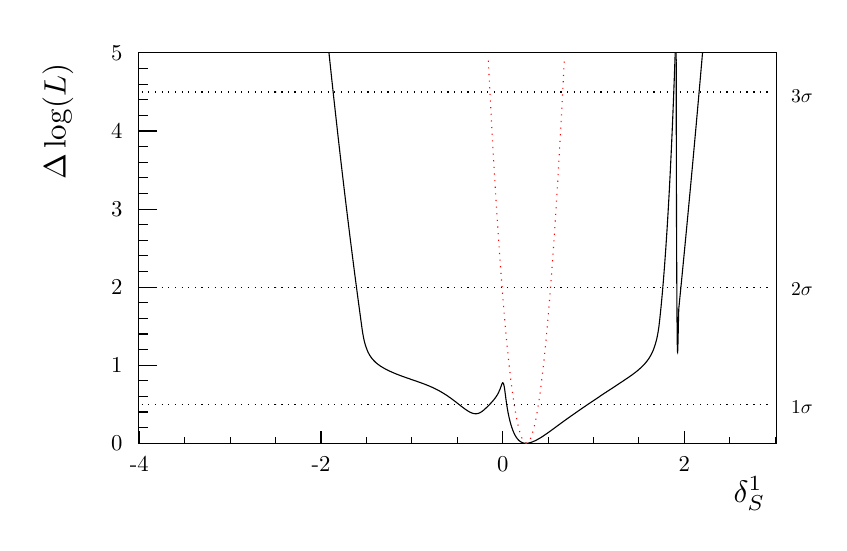
\begin{tikzpicture}
\pgfdeclareplotmark{cross} {
\pgfpathmoveto{\pgfpoint{-0.3\pgfplotmarksize}{\pgfplotmarksize}}
\pgfpathlineto{\pgfpoint{+0.3\pgfplotmarksize}{\pgfplotmarksize}}
\pgfpathlineto{\pgfpoint{+0.3\pgfplotmarksize}{0.3\pgfplotmarksize}}
\pgfpathlineto{\pgfpoint{+1\pgfplotmarksize}{0.3\pgfplotmarksize}}
\pgfpathlineto{\pgfpoint{+1\pgfplotmarksize}{-0.3\pgfplotmarksize}}
\pgfpathlineto{\pgfpoint{+0.3\pgfplotmarksize}{-0.3\pgfplotmarksize}}
\pgfpathlineto{\pgfpoint{+0.3\pgfplotmarksize}{-1.\pgfplotmarksize}}
\pgfpathlineto{\pgfpoint{-0.3\pgfplotmarksize}{-1.\pgfplotmarksize}}
\pgfpathlineto{\pgfpoint{-0.3\pgfplotmarksize}{-0.3\pgfplotmarksize}}
\pgfpathlineto{\pgfpoint{-1.\pgfplotmarksize}{-0.3\pgfplotmarksize}}
\pgfpathlineto{\pgfpoint{-1.\pgfplotmarksize}{0.3\pgfplotmarksize}}
\pgfpathlineto{\pgfpoint{-0.3\pgfplotmarksize}{0.3\pgfplotmarksize}}
\pgfpathclose
\pgfusepathqstroke
}
\pgfdeclareplotmark{cross*} {
\pgfpathmoveto{\pgfpoint{-0.3\pgfplotmarksize}{\pgfplotmarksize}}
\pgfpathlineto{\pgfpoint{+0.3\pgfplotmarksize}{\pgfplotmarksize}}
\pgfpathlineto{\pgfpoint{+0.3\pgfplotmarksize}{0.3\pgfplotmarksize}}
\pgfpathlineto{\pgfpoint{+1\pgfplotmarksize}{0.3\pgfplotmarksize}}
\pgfpathlineto{\pgfpoint{+1\pgfplotmarksize}{-0.3\pgfplotmarksize}}
\pgfpathlineto{\pgfpoint{+0.3\pgfplotmarksize}{-0.3\pgfplotmarksize}}
\pgfpathlineto{\pgfpoint{+0.3\pgfplotmarksize}{-1.\pgfplotmarksize}}
\pgfpathlineto{\pgfpoint{-0.3\pgfplotmarksize}{-1.\pgfplotmarksize}}
\pgfpathlineto{\pgfpoint{-0.3\pgfplotmarksize}{-0.3\pgfplotmarksize}}
\pgfpathlineto{\pgfpoint{-1.\pgfplotmarksize}{-0.3\pgfplotmarksize}}
\pgfpathlineto{\pgfpoint{-1.\pgfplotmarksize}{0.3\pgfplotmarksize}}
\pgfpathlineto{\pgfpoint{-0.3\pgfplotmarksize}{0.3\pgfplotmarksize}}
\pgfpathclose
\pgfusepathqfillstroke
}
\pgfdeclareplotmark{newstar} {
\pgfpathmoveto{\pgfqpoint{0pt}{\pgfplotmarksize}}
\pgfpathlineto{\pgfqpointpolar{44}{0.5\pgfplotmarksize}}
\pgfpathlineto{\pgfqpointpolar{18}{\pgfplotmarksize}}
\pgfpathlineto{\pgfqpointpolar{-20}{0.5\pgfplotmarksize}}
\pgfpathlineto{\pgfqpointpolar{-54}{\pgfplotmarksize}}
\pgfpathlineto{\pgfqpointpolar{-90}{0.5\pgfplotmarksize}}
\pgfpathlineto{\pgfqpointpolar{234}{\pgfplotmarksize}}
\pgfpathlineto{\pgfqpointpolar{198}{0.5\pgfplotmarksize}}
\pgfpathlineto{\pgfqpointpolar{162}{\pgfplotmarksize}}
\pgfpathlineto{\pgfqpointpolar{134}{0.5\pgfplotmarksize}}
\pgfpathclose
\pgfusepathqstroke
}
\pgfdeclareplotmark{newstar*} {
\pgfpathmoveto{\pgfqpoint{0pt}{\pgfplotmarksize}}
\pgfpathlineto{\pgfqpointpolar{44}{0.5\pgfplotmarksize}}
\pgfpathlineto{\pgfqpointpolar{18}{\pgfplotmarksize}}
\pgfpathlineto{\pgfqpointpolar{-20}{0.5\pgfplotmarksize}}
\pgfpathlineto{\pgfqpointpolar{-54}{\pgfplotmarksize}}
\pgfpathlineto{\pgfqpointpolar{-90}{0.5\pgfplotmarksize}}
\pgfpathlineto{\pgfqpointpolar{234}{\pgfplotmarksize}}
\pgfpathlineto{\pgfqpointpolar{198}{0.5\pgfplotmarksize}}
\pgfpathlineto{\pgfqpointpolar{162}{\pgfplotmarksize}}
\pgfpathlineto{\pgfqpointpolar{134}{0.5\pgfplotmarksize}}
\pgfpathclose
\pgfusepathqfillstroke
}
\definecolor{c}{rgb}{1,1,1};
\draw [color=c, fill=c] (0,0) rectangle (10,6.27517);
\draw [color=c, fill=c] (1.4,1.00403) rectangle (9.5,5.96141);
\definecolor{c}{rgb}{0,0,0};
\draw [c] (1.4,1.00403) -- (1.4,5.96141) -- (9.5,5.96141) -- (9.5,1.00403) -- (1.4,1.00403);
\draw [c,line width=0.4] (1.4,1.00403) -- (9.5,1.00403);
\draw [anchor= east] (9.5,0.36145) node[scale=1.11794, rotate=0]{$\delta_{S}^{1}$};
\draw [c,line width=0.4] (1.41142,1.15651) -- (1.41142,1.00403);
\draw [c,line width=0.4] (1.98818,1.08027) -- (1.98818,1.00403);
\draw [c,line width=0.4] (2.56495,1.08027) -- (2.56495,1.00403);
\draw [c,line width=0.4] (3.14171,1.08027) -- (3.14171,1.00403);
\draw [c,line width=0.4] (3.71848,1.15651) -- (3.71848,1.00403);
\draw [c,line width=0.4] (4.29524,1.08027) -- (4.29524,1.00403);
\draw [c,line width=0.4] (4.87201,1.08027) -- (4.87201,1.00403);
\draw [c,line width=0.4] (5.44877,1.08027) -- (5.44877,1.00403);
\draw [c,line width=0.4] (6.02554,1.15651) -- (6.02554,1.00403);
\draw [c,line width=0.4] (6.6023,1.08027) -- (6.6023,1.00403);
\draw [c,line width=0.4] (7.17907,1.08027) -- (7.17907,1.00403);
\draw [c,line width=0.4] (7.75583,1.08027) -- (7.75583,1.00403);
\draw [c,line width=0.4] (8.3326,1.15651) -- (8.3326,1.00403);
\draw [c,line width=0.4] (1.41142,1.15651) -- (1.41142,1.00403);
\draw [c,line width=0.4] (8.3326,1.15651) -- (8.3326,1.00403);
\draw [c,line width=0.4] (8.90936,1.08027) -- (8.90936,1.00403);
\draw [c,line width=0.4] (9.48613,1.08027) -- (9.48613,1.00403);
\draw [anchor=base] (1.41142,0.640067) node[scale=0.819821, rotate=0]{-4};
\draw [anchor=base] (3.71848,0.640067) node[scale=0.819821, rotate=0]{-2};
\draw [anchor=base] (6.02554,0.640067) node[scale=0.819821, rotate=0]{0};
\draw [anchor=base] (8.3326,0.640067) node[scale=0.819821, rotate=0]{2};
\draw [c,line width=0.4] (1.4,1.00403) -- (1.4,5.96141);
\draw [anchor= east] (0.376,5.96141) node[scale=1.11794, rotate=90]{$\Delta\log(\text{L})$};
\draw [c,line width=0.4] (1.637,1.00403) -- (1.4,1.00403);
\draw [c,line width=0.4] (1.5185,1.20232) -- (1.4,1.20232);
\draw [c,line width=0.4] (1.5185,1.40062) -- (1.4,1.40062);
\draw [c,line width=0.4] (1.5185,1.59891) -- (1.4,1.59891);
\draw [c,line width=0.4] (1.5185,1.79721) -- (1.4,1.79721);
\draw [c,line width=0.4] (1.637,1.9955) -- (1.4,1.9955);
\draw [c,line width=0.4] (1.5185,2.1938) -- (1.4,2.1938);
\draw [c,line width=0.4] (1.5185,2.39209) -- (1.4,2.39209);
\draw [c,line width=0.4] (1.5185,2.59039) -- (1.4,2.59039);
\draw [c,line width=0.4] (1.5185,2.78868) -- (1.4,2.78868);
\draw [c,line width=0.4] (1.637,2.98698) -- (1.4,2.98698);
\draw [c,line width=0.4] (1.5185,3.18528) -- (1.4,3.18528);
\draw [c,line width=0.4] (1.5185,3.38357) -- (1.4,3.38357);
\draw [c,line width=0.4] (1.5185,3.58187) -- (1.4,3.58187);
\draw [c,line width=0.4] (1.5185,3.78016) -- (1.4,3.78016);
\draw [c,line width=0.4] (1.637,3.97846) -- (1.4,3.97846);
\draw [c,line width=0.4] (1.5185,4.17675) -- (1.4,4.17675);
\draw [c,line width=0.4] (1.5185,4.37505) -- (1.4,4.37505);
\draw [c,line width=0.4] (1.5185,4.57334) -- (1.4,4.57334);
\draw [c,line width=0.4] (1.5185,4.77164) -- (1.4,4.77164);
\draw [c,line width=0.4] (1.637,4.96993) -- (1.4,4.96993);
\draw [c,line width=0.4] (1.5185,5.16823) -- (1.4,5.16823);
\draw [c,line width=0.4] (1.5185,5.36652) -- (1.4,5.36652);
\draw [c,line width=0.4] (1.5185,5.56482) -- (1.4,5.56482);
\draw [c,line width=0.4] (1.5185,5.76311) -- (1.4,5.76311);
\draw [c,line width=0.4] (1.637,5.96141) -- (1.4,5.96141);
\draw [anchor= east] (1.3,1.00403) node[scale=0.819821, rotate=0]{0};
\draw [anchor= east] (1.3,1.9955) node[scale=0.819821, rotate=0]{1};
\draw [anchor= east] (1.3,2.98698) node[scale=0.819821, rotate=0]{2};
\draw [anchor= east] (1.3,3.97846) node[scale=0.819821, rotate=0]{3};
\draw [anchor= east] (1.3,4.96993) node[scale=0.819821, rotate=0]{4};
\draw [anchor= east] (1.3,5.96141) node[scale=0.819821, rotate=0]{5};
\draw [c,line width=0.4] (3.81954,5.96141) -- (3.8223,5.93501);
\draw [c,line width=0.4] (3.8223,5.93501) -- (3.83383,5.82555) -- (3.84537,5.71692) -- (3.8569,5.60886) -- (3.86844,5.50184) -- (3.87997,5.39563) -- (3.90304,5.18578) -- (3.91458,5.08214) -- (3.92612,4.97923) -- (3.93765,4.87723) -- (3.94919,4.77578)
 -- (3.96072,4.67509) -- (3.97226,4.57515) -- (3.98379,4.47594) -- (3.99533,4.37769) -- (4.00686,4.27998) -- (4.0184,4.1829) -- (4.02993,4.08697) -- (4.053,3.89705) -- (4.06454,3.80273) -- (4.07607,3.70963) -- (4.08761,3.61698) -- (4.09914,3.52504)
 -- (4.11068,3.43418) -- (4.12222,3.34367) -- (4.13375,3.25375) -- (4.14529,3.16451) -- (4.15682,3.0762) -- (4.16836,2.98837) -- (4.17989,2.90116) -- (4.19143,2.81424) -- (4.2145,2.64345) -- (4.22603,2.55842) -- (4.23757,2.47361) -- (4.2491,2.39679)
 -- (4.26064,2.33474) -- (4.27217,2.2852) -- (4.28371,2.24448) -- (4.30678,2.18085) -- (4.31832,2.15596) -- (4.32985,2.13422) -- (4.34139,2.11503) -- (4.35292,2.09793) -- (4.36446,2.08255) -- (4.37599,2.06861) -- (4.38753,2.05589) --
 (4.39906,2.04418) -- (4.4106,2.03257) -- (4.42213,2.02251) -- (4.4452,2.00421) -- (4.45674,1.99582) -- (4.46827,1.98785) -- (4.47981,1.98025) -- (4.49134,1.97299) -- (4.50288,1.96603) -- (4.51442,1.95933) -- (4.52595,1.95288) -- (4.53749,1.94664) --
 (4.54902,1.9406) -- (4.57209,1.92906) -- (4.58363,1.92352) -- (4.59516,1.91812) -- (4.6067,1.91285) -- (4.61823,1.9077) -- (4.62977,1.90266) -- (4.6413,1.89773) -- (4.65284,1.89289) -- (4.66437,1.88814) -- (4.67591,1.88348) -- (4.68744,1.8789) --
 (4.69898,1.87438) -- (4.72205,1.86556) -- (4.73359,1.86123) -- (4.74512,1.85696) -- (4.75666,1.85274) -- (4.76819,1.84857) -- (4.77973,1.84443) -- (4.79126,1.84033) -- (4.8028,1.83627) -- (4.81433,1.83223) -- (4.82587,1.82821) -- (4.8374,1.82422) --
 (4.84894,1.82024) -- (4.86047,1.81627) -- (4.87201,1.81231) -- (4.88354,1.80835) -- (4.89508,1.80438) -- (4.90662,1.80041) -- (4.91815,1.79643) -- (4.92969,1.79243) -- (4.94122,1.78841) -- (4.95276,1.78436) -- (4.96429,1.78028) -- (4.98736,1.772) --
 (4.9989,1.7678) -- (5.01043,1.76353) -- (5.02197,1.75922) -- (5.0335,1.75483) -- (5.04504,1.75037) -- (5.05657,1.74583) -- (5.06811,1.74121) -- (5.07965,1.7365) -- (5.09118,1.73171) -- (5.10272,1.7268) -- (5.12579,1.71666) -- (5.13732,1.71142) --
 (5.14886,1.70605) -- (5.16039,1.70055) -- (5.17193,1.69491) -- (5.18346,1.68914) -- (5.195,1.68321) -- (5.20653,1.67714) -- (5.21807,1.67092) -- (5.2296,1.66454) -- (5.24114,1.658) -- (5.25267,1.65129) -- (5.26421,1.64443) -- (5.28728,1.6302) --
 (5.29882,1.62284) -- (5.31035,1.61532) -- (5.32189,1.60763) -- (5.33342,1.59979) -- (5.34496,1.59179) -- (5.36803,1.57537) -- (5.37956,1.56695) -- (5.3911,1.5584) -- (5.40263,1.54975) -- (5.41417,1.54099) -- (5.4257,1.53214) -- (5.43724,1.52322) --
 (5.44877,1.51425) -- (5.46031,1.50523) -- (5.47185,1.49621) -- (5.48338,1.4872) -- (5.49492,1.47822) -- (5.50645,1.46932) -- (5.51799,1.46052) -- (5.52952,1.45186) -- (5.54106,1.44339) -- (5.55259,1.43514) -- (5.56413,1.42718) -- (5.5872,1.41236) --
 (5.59873,1.40563) -- (5.61027,1.39946) -- (5.6218,1.39392) -- (5.63334,1.38911) -- (5.64487,1.38513) -- (5.65641,1.38205) -- (5.66795,1.37999) -- (5.67948,1.37902) -- (5.69102,1.37923) -- (5.70255,1.38066) -- (5.71409,1.38336) -- (5.72562,1.38734)
 -- (5.73716,1.39256) -- (5.74869,1.39898) -- (5.76023,1.40649) -- (5.77176,1.41498) -- (5.7833,1.42431) -- (5.79483,1.43432) -- (5.80637,1.44487) -- (5.8179,1.4558) -- (5.82944,1.46704) -- (5.84097,1.47851) -- (5.85251,1.49017) -- (5.86405,1.50204)
 -- (5.87558,1.51417) -- (5.88712,1.52665) -- (5.89865,1.53958) -- (5.91019,1.55313) -- (5.92172,1.5675) -- (5.93326,1.58294) -- (5.94479,1.59936) -- (5.95633,1.61761) -- (5.96786,1.63764) -- (5.99093,1.68841) -- (6.00247,1.72034) -- (6.014,1.75253)
 -- (6.02348,1.77091) -- (6.02554,1.77226) -- (6.03313,1.76767) -- (6.03708,1.75881) -- (6.04484,1.72599) -- (6.04861,1.7043) -- (6.06015,1.61702) -- (6.07168,1.52954) -- (6.08322,1.4537) -- (6.09475,1.3897) -- (6.10629,1.33414) -- (6.11782,1.28591)
 -- (6.12936,1.24367) -- (6.14089,1.20665) -- (6.15243,1.17416) -- (6.16396,1.14567) -- (6.1755,1.12024) -- (6.18703,1.0988) -- (6.19857,1.08017) -- (6.2101,1.06412) -- (6.22164,1.05045) -- (6.23318,1.03895) -- (6.24471,1.0294) -- (6.25625,1.02165)
 -- (6.26778,1.0155) -- (6.27932,1.01081) -- (6.29085,1.00744) -- (6.30239,1.00527) -- (6.31392,1.00403) -- (6.32546,1.00403) -- (6.33699,1.00476) -- (6.34853,1.00627) -- (6.36006,1.00849) -- (6.3716,1.01133) -- (6.38313,1.01473) -- (6.39467,1.01864)
 -- (6.4062,1.023) -- (6.41774,1.02775) -- (6.42928,1.03287) -- (6.44081,1.03832) -- (6.45235,1.04406) -- (6.46388,1.05005) -- (6.47542,1.05628) -- (6.49849,1.06979) -- (6.51002,1.07672) -- (6.52156,1.08381) -- (6.53309,1.09107) -- (6.54463,1.09924)
 -- (6.55616,1.10691) -- (6.5677,1.11472) -- (6.57923,1.12264) -- (6.59077,1.13067) -- (6.6023,1.13879) -- (6.61384,1.147) -- (6.62538,1.15528) -- (6.63691,1.16362) -- (6.64845,1.17201) -- (6.65998,1.18044) -- (6.67152,1.18891) -- (6.68305,1.1974) --
 (6.69459,1.20591) -- (6.70612,1.21443) -- (6.71766,1.22295) -- (6.72919,1.23146) -- (6.74073,1.23997) -- (6.75226,1.24847) -- (6.7638,1.25694) -- (6.77533,1.26531) -- (6.78687,1.27372) -- (6.7984,1.2821) -- (6.80994,1.29046) -- (6.83301,1.30706) --
 (6.84455,1.31532) -- (6.85608,1.32354) -- (6.86762,1.33174) -- (6.87915,1.3399) -- (6.89069,1.34803) -- (6.90222,1.35614) -- (6.91376,1.36422) -- (6.92529,1.37229) -- (6.93683,1.38034) -- (6.94836,1.38838) -- (6.9599,1.3964) -- (6.97143,1.40442) --
 (6.98297,1.41243) -- (6.9945,1.42045) -- (7.00604,1.42845) -- (7.02911,1.44443) -- (7.04065,1.45239) -- (7.05218,1.46031) -- (7.06372,1.46817) -- (7.07525,1.47594) -- (7.09832,1.49176) -- (7.10986,1.49958) -- (7.12139,1.5074) -- (7.13293,1.5152) --
 (7.14446,1.52299) -- (7.156,1.53077) -- (7.16753,1.53854) -- (7.17907,1.54628) -- (7.1906,1.55401) -- (7.20214,1.5617) -- (7.21368,1.56936) -- (7.23675,1.58456) -- (7.24828,1.59211) -- (7.25982,1.60057) -- (7.27135,1.60827) -- (7.28289,1.61596) --
 (7.29442,1.62328) -- (7.30596,1.63118) -- (7.31749,1.63893) -- (7.32903,1.64653) -- (7.34056,1.6539) -- (7.3521,1.66186) -- (7.36363,1.66947) -- (7.3867,1.68379) -- (7.39824,1.69142) -- (7.40978,1.69907) -- (7.42131,1.70671) -- (7.43285,1.71436) --
 (7.44438,1.722) -- (7.45592,1.72963) -- (7.46745,1.73725) -- (7.47899,1.74485) -- (7.49052,1.75243) -- (7.50206,1.76002) -- (7.52513,1.77526) -- (7.53666,1.78279) -- (7.5482,1.7901) -- (7.55973,1.79831) -- (7.57127,1.806) -- (7.58281,1.81346) --
 (7.59434,1.82152) -- (7.60588,1.82934) -- (7.61741,1.83655) -- (7.62895,1.84498) -- (7.64048,1.85319) -- (7.65202,1.86116) -- (7.67509,1.87761) -- (7.68662,1.88623) -- (7.69816,1.89522) -- (7.70969,1.9039) -- (7.72123,1.9131) -- (7.73276,1.92235) --
 (7.75583,1.94106) -- (7.76737,1.9517) -- (7.77891,1.96211) -- (7.79044,1.97226) -- (7.80198,1.98424) -- (7.81351,1.99571) -- (7.82505,2.00787) -- (7.83658,2.02136) -- (7.85965,2.04963) -- (7.87119,2.06545) -- (7.88272,2.08203) -- (7.89426,2.10056)
 -- (7.90579,2.12044) -- (7.91733,2.1423) -- (7.92886,2.16648) -- (7.9404,2.19367) -- (7.96347,2.25978) -- (7.9805,2.32304) -- (7.98654,2.3501) -- (7.99808,2.40999) -- (8.00961,2.48489) -- (8.02115,2.58592) -- (8.03663,2.73501) -- (8.05188,2.89755)
 -- (8.06698,3.07445) -- (8.08199,3.26682) -- (8.09694,3.47568) -- (8.1118,3.70143) -- (8.12647,3.9432) -- (8.14078,4.19859) -- (8.15576,4.48834) -- (8.1681,4.74612) -- (8.18118,5.03994) -- (8.19367,5.34273) -- (8.20625,5.67227) -- (8.21647,5.96141);
\draw [c,line width=0.4] (8.22904,5.96141) -- (8.22913,5.85045);
\draw [c,line width=0.4] (8.22913,5.85045) -- (8.22937,5.61918) -- (8.22967,5.39466) -- (8.23001,5.17589) -- (8.23038,4.96188) -- (8.23081,4.75165) -- (8.23128,4.54437) -- (8.2318,4.33952) -- (8.23237,4.13713) -- (8.23299,3.93802) -- (8.23365,3.744)
 -- (8.23436,3.55755) -- (8.23516,3.3665) -- (8.23588,3.2115) -- (8.23669,3.05066) -- (8.23753,2.90095) -- (8.23844,2.75334) -- (8.23928,2.63222) -- (8.24018,2.51474) -- (8.24032,2.49811) -- (8.24102,2.41941) -- (8.24175,2.35127) -- (8.24251,2.29357)
 -- (8.24329,2.24624) -- (8.2441,2.20929) -- (8.24505,2.1803) -- (8.24601,2.16496) -- (8.24699,2.16192) -- (8.24803,2.17086) -- (8.24918,2.19288) -- (8.25049,2.23106) -- (8.25204,2.28991) -- (8.25448,2.40031) -- (8.25784,2.55911) -- (8.25961,2.63237)
 -- (8.26092,2.67712) -- (8.26206,2.70676) -- (8.26321,2.72613) -- (8.26339,2.72809) -- (8.27492,2.8445) -- (8.28646,2.96115) -- (8.29799,3.07811) -- (8.30953,3.19598) -- (8.32106,3.31466) -- (8.3326,3.43381) -- (8.34414,3.55362) -- (8.35567,3.67422)
 -- (8.36721,3.79505) -- (8.37874,3.91678) -- (8.39028,4.03912) -- (8.40181,4.16223) -- (8.41335,4.28601) -- (8.42488,4.41023) -- (8.43642,4.53546) -- (8.44795,4.66127) -- (8.45949,4.78741) -- (8.47102,4.91495) -- (8.48256,5.04294) --
 (8.50563,5.30175) -- (8.51716,5.43187) -- (8.5287,5.56269) -- (8.54024,5.69425) -- (8.55177,5.82653) -- (8.56331,5.95947) -- (8.56347,5.96141);
\draw [c,dotted] (1.4405,1.49977) -- (1.5215,1.49977) -- (1.6025,1.49977) -- (1.6835,1.49977) -- (1.7645,1.49977) -- (1.8455,1.49977) -- (1.9265,1.49977) -- (2.0075,1.49977) -- (2.0885,1.49977) -- (2.1695,1.49977) -- (2.2505,1.49977) --
 (2.3315,1.49977) -- (2.4125,1.49977) -- (2.4935,1.49977) -- (2.5745,1.49977) -- (2.6555,1.49977) -- (2.7365,1.49977) -- (2.8175,1.49977) -- (2.8985,1.49977) -- (2.9795,1.49977) -- (3.0605,1.49977) -- (3.1415,1.49977) -- (3.2225,1.49977) --
 (3.3035,1.49977) -- (3.3845,1.49977) -- (3.4655,1.49977) -- (3.5465,1.49977) -- (3.6275,1.49977) -- (3.7085,1.49977) -- (3.7895,1.49977) -- (3.8705,1.49977) -- (3.9515,1.49977) -- (4.0325,1.49977) -- (4.1135,1.49977) -- (4.1945,1.49977) --
 (4.2755,1.49977) -- (4.3565,1.49977) -- (4.4375,1.49977) -- (4.5185,1.49977) -- (4.5995,1.49977) -- (4.6805,1.49977) -- (4.7615,1.49977) -- (4.8425,1.49977) -- (4.9235,1.49977) -- (5.0045,1.49977) -- (5.0855,1.49977) -- (5.1665,1.49977) --
 (5.2475,1.49977) -- (5.3285,1.49977) -- (5.4095,1.49977);
\draw [c,dotted] (5.4095,1.49977) -- (5.4905,1.49977) -- (5.5715,1.49977) -- (5.6525,1.49977) -- (5.7335,1.49977) -- (5.8145,1.49977) -- (5.8955,1.49977) -- (5.9765,1.49977) -- (6.0575,1.49977) -- (6.1385,1.49977) -- (6.2195,1.49977) --
 (6.3005,1.49977) -- (6.3815,1.49977) -- (6.4625,1.49977) -- (6.5435,1.49977) -- (6.6245,1.49977) -- (6.7055,1.49977) -- (6.7865,1.49977) -- (6.8675,1.49977) -- (6.9485,1.49977) -- (7.0295,1.49977) -- (7.1105,1.49977) -- (7.1915,1.49977) --
 (7.2725,1.49977) -- (7.3535,1.49977) -- (7.4345,1.49977) -- (7.5155,1.49977) -- (7.5965,1.49977) -- (7.6775,1.49977) -- (7.7585,1.49977) -- (7.8395,1.49977) -- (7.9205,1.49977) -- (8.0015,1.49977) -- (8.0825,1.49977) -- (8.1635,1.49977) --
 (8.2445,1.49977) -- (8.3255,1.49977) -- (8.4065,1.49977) -- (8.4875,1.49977) -- (8.5685,1.49977) -- (8.6495,1.49977) -- (8.7305,1.49977) -- (8.8115,1.49977) -- (8.8925,1.49977) -- (8.9735,1.49977) -- (9.0545,1.49977) -- (9.1355,1.49977) --
 (9.2165,1.49977) -- (9.2975,1.49977) -- (9.3785,1.49977);
\draw [c,dotted] (9.3785,1.49977) -- (9.4595,1.49977);
\draw [c,dotted] (1.4405,2.98698) -- (1.5215,2.98698) -- (1.6025,2.98698) -- (1.6835,2.98698) -- (1.7645,2.98698) -- (1.8455,2.98698) -- (1.9265,2.98698) -- (2.0075,2.98698) -- (2.0885,2.98698) -- (2.1695,2.98698) -- (2.2505,2.98698) --
 (2.3315,2.98698) -- (2.4125,2.98698) -- (2.4935,2.98698) -- (2.5745,2.98698) -- (2.6555,2.98698) -- (2.7365,2.98698) -- (2.8175,2.98698) -- (2.8985,2.98698) -- (2.9795,2.98698) -- (3.0605,2.98698) -- (3.1415,2.98698) -- (3.2225,2.98698) --
 (3.3035,2.98698) -- (3.3845,2.98698) -- (3.4655,2.98698) -- (3.5465,2.98698) -- (3.6275,2.98698) -- (3.7085,2.98698) -- (3.7895,2.98698) -- (3.8705,2.98698) -- (3.9515,2.98698) -- (4.0325,2.98698) -- (4.1135,2.98698) -- (4.1945,2.98698) --
 (4.2755,2.98698) -- (4.3565,2.98698) -- (4.4375,2.98698) -- (4.5185,2.98698) -- (4.5995,2.98698) -- (4.6805,2.98698) -- (4.7615,2.98698) -- (4.8425,2.98698) -- (4.9235,2.98698) -- (5.0045,2.98698) -- (5.0855,2.98698) -- (5.1665,2.98698) --
 (5.2475,2.98698) -- (5.3285,2.98698) -- (5.4095,2.98698);
\draw [c,dotted] (5.4095,2.98698) -- (5.4905,2.98698) -- (5.5715,2.98698) -- (5.6525,2.98698) -- (5.7335,2.98698) -- (5.8145,2.98698) -- (5.8955,2.98698) -- (5.9765,2.98698) -- (6.0575,2.98698) -- (6.1385,2.98698) -- (6.2195,2.98698) --
 (6.3005,2.98698) -- (6.3815,2.98698) -- (6.4625,2.98698) -- (6.5435,2.98698) -- (6.6245,2.98698) -- (6.7055,2.98698) -- (6.7865,2.98698) -- (6.8675,2.98698) -- (6.9485,2.98698) -- (7.0295,2.98698) -- (7.1105,2.98698) -- (7.1915,2.98698) --
 (7.2725,2.98698) -- (7.3535,2.98698) -- (7.4345,2.98698) -- (7.5155,2.98698) -- (7.5965,2.98698) -- (7.6775,2.98698) -- (7.7585,2.98698) -- (7.8395,2.98698) -- (7.9205,2.98698) -- (8.0015,2.98698) -- (8.0825,2.98698) -- (8.1635,2.98698) --
 (8.2445,2.98698) -- (8.3255,2.98698) -- (8.4065,2.98698) -- (8.4875,2.98698) -- (8.5685,2.98698) -- (8.6495,2.98698) -- (8.7305,2.98698) -- (8.8115,2.98698) -- (8.8925,2.98698) -- (8.9735,2.98698) -- (9.0545,2.98698) -- (9.1355,2.98698) --
 (9.2165,2.98698) -- (9.2975,2.98698) -- (9.3785,2.98698);
\draw [c,dotted] (9.3785,2.98698) -- (9.4595,2.98698);
\draw [c,dotted] (1.4405,5.46567) -- (1.5215,5.46567) -- (1.6025,5.46567) -- (1.6835,5.46567) -- (1.7645,5.46567) -- (1.8455,5.46567) -- (1.9265,5.46567) -- (2.0075,5.46567) -- (2.0885,5.46567) -- (2.1695,5.46567) -- (2.2505,5.46567) --
 (2.3315,5.46567) -- (2.4125,5.46567) -- (2.4935,5.46567) -- (2.5745,5.46567) -- (2.6555,5.46567) -- (2.7365,5.46567) -- (2.8175,5.46567) -- (2.8985,5.46567) -- (2.9795,5.46567) -- (3.0605,5.46567) -- (3.1415,5.46567) -- (3.2225,5.46567) --
 (3.3035,5.46567) -- (3.3845,5.46567) -- (3.4655,5.46567) -- (3.5465,5.46567) -- (3.6275,5.46567) -- (3.7085,5.46567) -- (3.7895,5.46567) -- (3.8705,5.46567) -- (3.9515,5.46567) -- (4.0325,5.46567) -- (4.1135,5.46567) -- (4.1945,5.46567) --
 (4.2755,5.46567) -- (4.3565,5.46567) -- (4.4375,5.46567) -- (4.5185,5.46567) -- (4.5995,5.46567) -- (4.6805,5.46567) -- (4.7615,5.46567) -- (4.8425,5.46567) -- (4.9235,5.46567) -- (5.0045,5.46567) -- (5.0855,5.46567) -- (5.1665,5.46567) --
 (5.2475,5.46567) -- (5.3285,5.46567) -- (5.4095,5.46567);
\draw [c,dotted] (5.4095,5.46567) -- (5.4905,5.46567) -- (5.5715,5.46567) -- (5.6525,5.46567) -- (5.7335,5.46567) -- (5.8145,5.46567) -- (5.8955,5.46567) -- (5.9765,5.46567) -- (6.0575,5.46567) -- (6.1385,5.46567) -- (6.2195,5.46567) --
 (6.3005,5.46567) -- (6.3815,5.46567) -- (6.4625,5.46567) -- (6.5435,5.46567) -- (6.6245,5.46567) -- (6.7055,5.46567) -- (6.7865,5.46567) -- (6.8675,5.46567) -- (6.9485,5.46567) -- (7.0295,5.46567) -- (7.1105,5.46567) -- (7.1915,5.46567) --
 (7.2725,5.46567) -- (7.3535,5.46567) -- (7.4345,5.46567) -- (7.5155,5.46567) -- (7.5965,5.46567) -- (7.6775,5.46567) -- (7.7585,5.46567) -- (7.8395,5.46567) -- (7.9205,5.46567) -- (8.0015,5.46567) -- (8.0825,5.46567) -- (8.1635,5.46567) --
 (8.2445,5.46567) -- (8.3255,5.46567) -- (8.4065,5.46567) -- (8.4875,5.46567) -- (8.5685,5.46567) -- (8.6495,5.46567) -- (8.7305,5.46567) -- (8.8115,5.46567) -- (8.8925,5.46567) -- (8.9735,5.46567) -- (9.0545,5.46567) -- (9.1355,5.46567) --
 (9.2165,5.46567) -- (9.2975,5.46567) -- (9.3785,5.46567);
\draw [c,dotted] (9.3785,5.46567) -- (9.4595,5.46567);
\definecolor{c}{rgb}{1,0,0};
\draw [c,dotted] (5.84318,5.86276) -- (5.85293,5.66843) -- (5.86267,5.47806) -- (5.87241,5.29167) -- (5.88216,5.10924) -- (5.8919,4.93077) -- (5.90164,4.75627) -- (5.91138,4.58574) -- (5.92113,4.41917) -- (5.93087,4.25657) -- (5.94061,4.09793) --
 (5.95036,3.94326) -- (5.9601,3.79255) -- (5.96984,3.64582) -- (5.97959,3.50304) -- (5.98933,3.36424) -- (5.99907,3.2294) -- (6.00881,3.09852) -- (6.01856,2.97161) -- (6.0283,2.84867) -- (6.03804,2.72969) -- (6.04779,2.61468) -- (6.05753,2.50364) --
 (6.06727,2.39656) -- (6.07701,2.29344) -- (6.08676,2.19429) -- (6.0965,2.09911) -- (6.10624,2.0079) -- (6.11599,1.92065) -- (6.12573,1.83736) -- (6.13547,1.75804) -- (6.14521,1.68269) -- (6.15496,1.61131) -- (6.1647,1.54389) -- (6.17444,1.48043) --
 (6.18419,1.42094) -- (6.19393,1.36542) -- (6.20367,1.31386) -- (6.21341,1.26627) -- (6.22316,1.22265) -- (6.2329,1.18299) -- (6.24264,1.1473) -- (6.25239,1.11557) -- (6.26213,1.08781) -- (6.27187,1.06401) -- (6.28161,1.04418) -- (6.29136,1.02832) --
 (6.3011,1.01642) -- (6.31084,1.00849) -- (6.32059,1.00403);
\draw [c,dotted] (6.32059,1.00403) -- (6.33033,1.00452) -- (6.34007,1.00849) -- (6.34981,1.01642) -- (6.35956,1.02832) -- (6.3693,1.04418) -- (6.37904,1.06401) -- (6.38879,1.08781) -- (6.39853,1.11557) -- (6.40827,1.1473) -- (6.41802,1.18299) --
 (6.42776,1.22265) -- (6.4375,1.26627) -- (6.44724,1.31386) -- (6.45699,1.36542) -- (6.46673,1.42094) -- (6.47647,1.48043) -- (6.48622,1.54389) -- (6.49596,1.61131) -- (6.5057,1.68269) -- (6.51544,1.75804) -- (6.52519,1.83736) -- (6.53493,1.92065) --
 (6.54467,2.0079) -- (6.55442,2.09911) -- (6.56416,2.19429) -- (6.5739,2.29344) -- (6.58364,2.39656) -- (6.59339,2.50364) -- (6.60313,2.61468) -- (6.61287,2.72969) -- (6.62262,2.84867) -- (6.63236,2.97161) -- (6.6421,3.09852) -- (6.65184,3.2294) --
 (6.66159,3.36424) -- (6.67133,3.50304) -- (6.68107,3.64582) -- (6.69082,3.79255) -- (6.70056,3.94326) -- (6.7103,4.09793) -- (6.72004,4.25657) -- (6.72979,4.41917) -- (6.73953,4.58574) -- (6.74927,4.75627) -- (6.75902,4.93077) -- (6.76876,5.10924)
 -- (6.7785,5.29167) -- (6.78824,5.47806) -- (6.79799,5.66843);
\draw [c,dotted] (6.79799,5.66843) -- (6.80773,5.86276);
\draw [anchor=base west] (9.6,1.38054) node[scale=0.708027, rotate=0]{$1\sigma$};
\draw [anchor=base west] (9.6,2.88658) node[scale=0.708027, rotate=0]{$2\sigma$};
\draw [anchor=base west] (9.6,5.33389) node[scale=0.708027, rotate=0]{$3\sigma$};
\end{tikzpicture}
}
    \caption{}
    \label{nll_ASPhase_bin1}
  \end{subfigure}
  \begin{subfigure}{0.5\textwidth}
    \tikzsetnextfilename{nll_ASMag2_bin2} 
    \scalebox{0.60}{\begin{tikzpicture}
\pgfdeclareplotmark{cross} {
\pgfpathmoveto{\pgfpoint{-0.3\pgfplotmarksize}{\pgfplotmarksize}}
\pgfpathlineto{\pgfpoint{+0.3\pgfplotmarksize}{\pgfplotmarksize}}
\pgfpathlineto{\pgfpoint{+0.3\pgfplotmarksize}{0.3\pgfplotmarksize}}
\pgfpathlineto{\pgfpoint{+1\pgfplotmarksize}{0.3\pgfplotmarksize}}
\pgfpathlineto{\pgfpoint{+1\pgfplotmarksize}{-0.3\pgfplotmarksize}}
\pgfpathlineto{\pgfpoint{+0.3\pgfplotmarksize}{-0.3\pgfplotmarksize}}
\pgfpathlineto{\pgfpoint{+0.3\pgfplotmarksize}{-1.\pgfplotmarksize}}
\pgfpathlineto{\pgfpoint{-0.3\pgfplotmarksize}{-1.\pgfplotmarksize}}
\pgfpathlineto{\pgfpoint{-0.3\pgfplotmarksize}{-0.3\pgfplotmarksize}}
\pgfpathlineto{\pgfpoint{-1.\pgfplotmarksize}{-0.3\pgfplotmarksize}}
\pgfpathlineto{\pgfpoint{-1.\pgfplotmarksize}{0.3\pgfplotmarksize}}
\pgfpathlineto{\pgfpoint{-0.3\pgfplotmarksize}{0.3\pgfplotmarksize}}
\pgfpathclose
\pgfusepathqstroke
}
\pgfdeclareplotmark{cross*} {
\pgfpathmoveto{\pgfpoint{-0.3\pgfplotmarksize}{\pgfplotmarksize}}
\pgfpathlineto{\pgfpoint{+0.3\pgfplotmarksize}{\pgfplotmarksize}}
\pgfpathlineto{\pgfpoint{+0.3\pgfplotmarksize}{0.3\pgfplotmarksize}}
\pgfpathlineto{\pgfpoint{+1\pgfplotmarksize}{0.3\pgfplotmarksize}}
\pgfpathlineto{\pgfpoint{+1\pgfplotmarksize}{-0.3\pgfplotmarksize}}
\pgfpathlineto{\pgfpoint{+0.3\pgfplotmarksize}{-0.3\pgfplotmarksize}}
\pgfpathlineto{\pgfpoint{+0.3\pgfplotmarksize}{-1.\pgfplotmarksize}}
\pgfpathlineto{\pgfpoint{-0.3\pgfplotmarksize}{-1.\pgfplotmarksize}}
\pgfpathlineto{\pgfpoint{-0.3\pgfplotmarksize}{-0.3\pgfplotmarksize}}
\pgfpathlineto{\pgfpoint{-1.\pgfplotmarksize}{-0.3\pgfplotmarksize}}
\pgfpathlineto{\pgfpoint{-1.\pgfplotmarksize}{0.3\pgfplotmarksize}}
\pgfpathlineto{\pgfpoint{-0.3\pgfplotmarksize}{0.3\pgfplotmarksize}}
\pgfpathclose
\pgfusepathqfillstroke
}
\pgfdeclareplotmark{newstar} {
\pgfpathmoveto{\pgfqpoint{0pt}{\pgfplotmarksize}}
\pgfpathlineto{\pgfqpointpolar{44}{0.5\pgfplotmarksize}}
\pgfpathlineto{\pgfqpointpolar{18}{\pgfplotmarksize}}
\pgfpathlineto{\pgfqpointpolar{-20}{0.5\pgfplotmarksize}}
\pgfpathlineto{\pgfqpointpolar{-54}{\pgfplotmarksize}}
\pgfpathlineto{\pgfqpointpolar{-90}{0.5\pgfplotmarksize}}
\pgfpathlineto{\pgfqpointpolar{234}{\pgfplotmarksize}}
\pgfpathlineto{\pgfqpointpolar{198}{0.5\pgfplotmarksize}}
\pgfpathlineto{\pgfqpointpolar{162}{\pgfplotmarksize}}
\pgfpathlineto{\pgfqpointpolar{134}{0.5\pgfplotmarksize}}
\pgfpathclose
\pgfusepathqstroke
}
\pgfdeclareplotmark{newstar*} {
\pgfpathmoveto{\pgfqpoint{0pt}{\pgfplotmarksize}}
\pgfpathlineto{\pgfqpointpolar{44}{0.5\pgfplotmarksize}}
\pgfpathlineto{\pgfqpointpolar{18}{\pgfplotmarksize}}
\pgfpathlineto{\pgfqpointpolar{-20}{0.5\pgfplotmarksize}}
\pgfpathlineto{\pgfqpointpolar{-54}{\pgfplotmarksize}}
\pgfpathlineto{\pgfqpointpolar{-90}{0.5\pgfplotmarksize}}
\pgfpathlineto{\pgfqpointpolar{234}{\pgfplotmarksize}}
\pgfpathlineto{\pgfqpointpolar{198}{0.5\pgfplotmarksize}}
\pgfpathlineto{\pgfqpointpolar{162}{\pgfplotmarksize}}
\pgfpathlineto{\pgfqpointpolar{134}{0.5\pgfplotmarksize}}
\pgfpathclose
\pgfusepathqfillstroke
}
\definecolor{c}{rgb}{1,1,1};
\draw [color=c, fill=c] (0,0) rectangle (10,6.27517);
\draw [color=c, fill=c] (1.4,1.00403) rectangle (9.5,5.96141);
\definecolor{c}{rgb}{0,0,0};
\draw [c] (1.4,1.00403) -- (1.4,5.96141) -- (9.5,5.96141) -- (9.5,1.00403) -- (1.4,1.00403);
\draw [c,line width=0.4] (1.4,1.00403) -- (9.5,1.00403);
\draw [anchor= east] (9.5,0.200805) node[scale=1.37879, rotate=0]{$f_{S}^{2}$};
\draw [c,line width=0.4] (1.4,1.15651) -- (1.4,1.00403);
\draw [c,line width=0.4] (1.80913,1.08027) -- (1.80913,1.00403);
\draw [c,line width=0.4] (2.21826,1.08027) -- (2.21826,1.00403);
\draw [c,line width=0.4] (2.62739,1.08027) -- (2.62739,1.00403);
\draw [c,line width=0.4] (3.03651,1.15651) -- (3.03651,1.00403);
\draw [c,line width=0.4] (3.44564,1.08027) -- (3.44564,1.00403);
\draw [c,line width=0.4] (3.85477,1.08027) -- (3.85477,1.00403);
\draw [c,line width=0.4] (4.2639,1.08027) -- (4.2639,1.00403);
\draw [c,line width=0.4] (4.67303,1.15651) -- (4.67303,1.00403);
\draw [c,line width=0.4] (5.08216,1.08027) -- (5.08216,1.00403);
\draw [c,line width=0.4] (5.49129,1.08027) -- (5.49129,1.00403);
\draw [c,line width=0.4] (5.90041,1.08027) -- (5.90041,1.00403);
\draw [c,line width=0.4] (6.30954,1.15651) -- (6.30954,1.00403);
\draw [c,line width=0.4] (6.71867,1.08027) -- (6.71867,1.00403);
\draw [c,line width=0.4] (7.1278,1.08027) -- (7.1278,1.00403);
\draw [c,line width=0.4] (7.53693,1.08027) -- (7.53693,1.00403);
\draw [c,line width=0.4] (7.94606,1.15651) -- (7.94606,1.00403);
\draw [c,line width=0.4] (7.94606,1.15651) -- (7.94606,1.00403);
\draw [c,line width=0.4] (8.35519,1.08027) -- (8.35519,1.00403);
\draw [c,line width=0.4] (8.76431,1.08027) -- (8.76431,1.00403);
\draw [c,line width=0.4] (9.17344,1.08027) -- (9.17344,1.00403);
\draw [anchor=base] (1.4,0.602416) node[scale=1.11794, rotate=0]{0};
\draw [anchor=base] (3.03651,0.602416) node[scale=1.11794, rotate=0]{0.2};
\draw [anchor=base] (4.67303,0.602416) node[scale=1.11794, rotate=0]{0.4};
\draw [anchor=base] (6.30954,0.602416) node[scale=1.11794, rotate=0]{0.6};
\draw [anchor=base] (7.94606,0.602416) node[scale=1.11794, rotate=0]{0.8};
\draw [c,line width=0.4] (1.4,1.00403) -- (1.4,5.96141);
\draw [anchor= east] (0.28,5.96141) node[scale=1.37879, rotate=90]{$-\Delta\ln{L}$};
\draw [c,line width=0.4] (1.637,1.00403) -- (1.4,1.00403);
\draw [c,line width=0.4] (1.637,1.9955) -- (1.4,1.9955);
\draw [c,line width=0.4] (1.637,2.98698) -- (1.4,2.98698);
\draw [c,line width=0.4] (1.637,3.97846) -- (1.4,3.97846);
\draw [c,line width=0.4] (1.637,4.96993) -- (1.4,4.96993);
\draw [c,line width=0.4] (1.637,5.96141) -- (1.4,5.96141);
\draw [anchor= east] (1.4,1.00403) node[scale=1.11794, rotate=0]{0};
\draw [anchor= east] (1.4,1.9955) node[scale=1.11794, rotate=0]{1};
\draw [anchor= east] (1.4,2.98698) node[scale=1.11794, rotate=0]{2};
\draw [anchor= east] (1.4,3.97846) node[scale=1.11794, rotate=0]{3};
\draw [anchor= east] (1.4,4.96993) node[scale=1.11794, rotate=0]{4};
\draw [anchor= east] (1.4,5.96141) node[scale=1.11794, rotate=0]{5};
\draw [c,line width=0.4] (1.40736,3.14706) -- (1.41473,3.0632) -- (1.42209,2.99809) -- (1.42946,2.94251) -- (1.43682,2.89293) -- (1.44419,2.84756) -- (1.45155,2.80531) -- (1.45891,2.76549) -- (1.46628,2.72765) -- (1.47364,2.69142) --
 (1.48101,2.65656) -- (1.48837,2.62286) -- (1.49574,2.59017) -- (1.5031,2.55837) -- (1.51046,2.52735) -- (1.51783,2.49702) -- (1.52519,2.46733) -- (1.53256,2.4382) -- (1.53992,2.40959) -- (1.54729,2.38146) -- (1.55465,2.35377) -- (1.56201,2.32648) --
 (1.56938,2.29957) -- (1.57674,2.27302) -- (1.58411,2.2468) -- (1.59147,2.2209) -- (1.59884,2.1953) -- (1.6062,2.16998) -- (1.61357,2.14494) -- (1.62093,2.12016) -- (1.62829,2.09563) -- (1.63566,2.07135) -- (1.64302,2.04731) -- (1.65039,2.0235) --
 (1.65775,1.99992) -- (1.66512,1.97656) -- (1.67248,1.95342) -- (1.67984,1.9305) -- (1.68721,1.90779) -- (1.69457,1.8853) -- (1.70194,1.86301) -- (1.7093,1.84094) -- (1.71667,1.81908) -- (1.72403,1.79744) -- (1.73139,1.776) -- (1.73876,1.75478) --
 (1.74612,1.73377) -- (1.75349,1.71298) -- (1.76085,1.6924) -- (1.76822,1.67204) -- (1.77558,1.65191) -- (1.78294,1.632) -- (1.79031,1.61232) -- (1.79767,1.59287) -- (1.80504,1.57365) -- (1.8124,1.55467) -- (1.81977,1.53593) -- (1.82713,1.51743) --
 (1.83449,1.49919) -- (1.84186,1.48119) -- (1.84922,1.46345) -- (1.85659,1.445) -- (1.86395,1.42784) -- (1.87132,1.41095) -- (1.87868,1.39434) -- (1.88604,1.378) -- (1.89341,1.36194) -- (1.90077,1.34617) -- (1.90814,1.3313) -- (1.9155,1.31607) --
 (1.92287,1.30114) -- (1.93023,1.28651) -- (1.93759,1.2722) -- (1.94496,1.25821) -- (1.95232,1.24454) -- (1.95969,1.23119) -- (1.96705,1.21818) -- (1.97442,1.2055) -- (1.98178,1.19223) -- (1.98915,1.18034) -- (1.99651,1.16879) -- (2.00387,1.15759) --
 (2.01124,1.14674) -- (2.0186,1.13626) -- (2.02597,1.12613) -- (2.03333,1.11638) -- (2.0407,1.107) -- (2.04806,1.098) -- (2.05542,1.08938) -- (2.06279,1.08114) -- (2.07015,1.0733) -- (2.07752,1.06586) -- (2.08488,1.05881) -- (2.09225,1.05218) --
 (2.09961,1.04595) -- (2.10697,1.04013) -- (2.11434,1.03474) -- (2.1217,1.02977) -- (2.12907,1.02522) -- (2.13643,1.0211) -- (2.1438,1.01742) -- (2.15116,1.01418) -- (2.15852,1.01137) -- (2.16589,1.00902) -- (2.17325,1.00711) -- (2.18062,1.00565) --
 (2.18798,1.00465) -- (2.19535,1.00403) -- (2.20033,1.00519) -- (2.20271,1.00403) -- (2.21007,1.00403) -- (2.21744,1.00526) -- (2.2248,1.00658) -- (2.23217,1.00837) -- (2.23953,1.01063) -- (2.2469,1.01337) -- (2.25426,1.01659) -- (2.26162,1.02028) --
 (2.26899,1.02446) -- (2.27635,1.02912) -- (2.28372,1.03426) -- (2.29108,1.03989) -- (2.29845,1.046) -- (2.30581,1.0526) -- (2.31317,1.05969) -- (2.32054,1.06726) -- (2.3279,1.07532) -- (2.33527,1.08386) -- (2.34263,1.09289) -- (2.35,1.10241) --
 (2.35736,1.11298) -- (2.36473,1.12359) -- (2.37209,1.13471) -- (2.37945,1.14633) -- (2.38682,1.15845) -- (2.39418,1.17108) -- (2.40155,1.18422) -- (2.40891,1.19786) -- (2.41628,1.21202) -- (2.42364,1.22668) -- (2.431,1.24185) -- (2.43837,1.25753) --
 (2.44573,1.27372) -- (2.4531,1.29042) -- (2.46046,1.30764) -- (2.46783,1.32536) -- (2.47519,1.3436) -- (2.48255,1.36235) -- (2.48992,1.38161) -- (2.49728,1.40139) -- (2.50465,1.42167) -- (2.51201,1.44331) -- (2.51938,1.4647) -- (2.52674,1.48659) --
 (2.5341,1.50901) -- (2.54147,1.53194) -- (2.54883,1.55539) -- (2.5562,1.57935) -- (2.56356,1.60383) -- (2.57093,1.62882) -- (2.57829,1.65434) -- (2.58565,1.68036) -- (2.59302,1.70691) -- (2.60038,1.73397) -- (2.60775,1.76154) -- (2.61511,1.78963) --
 (2.62248,1.81823) -- (2.62984,1.84735) -- (2.6372,1.87698) -- (2.64457,1.90712) -- (2.65193,1.93778) -- (2.6593,1.96895) -- (2.66666,2.00064) -- (2.67403,2.03283) -- (2.68139,2.06553) -- (2.68875,2.09875) -- (2.69612,2.13248) -- (2.70348,2.16671) --
 (2.71085,2.20145) -- (2.71821,2.23671) -- (2.72558,2.27247) -- (2.73294,2.30873) -- (2.74031,2.34551) -- (2.74767,2.38277) -- (2.75503,2.42056) -- (2.7624,2.45885) -- (2.76976,2.49764) -- (2.77713,2.53693) -- (2.78449,2.57673) -- (2.79186,2.61703)
 -- (2.79922,2.65782) -- (2.80658,2.69912) -- (2.81395,2.74092) -- (2.82131,2.78321) -- (2.82868,2.82601) -- (2.83604,2.86929) -- (2.84341,2.91308) -- (2.85077,2.95736) -- (2.85813,3.00213) -- (2.8655,3.04739) -- (2.87286,3.09315) --
 (2.88023,3.13939) -- (2.88759,3.18613) -- (2.89496,3.23336) -- (2.90232,3.28107) -- (2.90968,3.32927) -- (2.91705,3.37795) -- (2.92441,3.42713) -- (2.93178,3.47678) -- (2.93914,3.52692) -- (2.94651,3.57754) -- (2.95387,3.62864) -- (2.96123,3.68022)
 -- (2.9686,3.73227) -- (2.97596,3.78481) -- (2.98333,3.83782) -- (2.99069,3.89131) -- (2.99806,3.94527) -- (3.00542,3.9997) -- (3.01278,4.05461) -- (3.02015,4.10999) -- (3.02751,4.16583) -- (3.03488,4.22215) -- (3.04224,4.27893) -- (3.04961,4.33618)
 -- (3.05697,4.39389) -- (3.06433,4.45207) -- (3.0717,4.51071) -- (3.07906,4.56981) -- (3.08643,4.62937) -- (3.09379,4.68939) -- (3.10116,4.74987) -- (3.10852,4.8108) -- (3.11589,4.87219) -- (3.12325,4.93403) -- (3.13061,4.99633) -- (3.13798,5.05907)
 -- (3.14534,5.12227) -- (3.15271,5.18591) -- (3.16007,5.25) -- (3.16744,5.31454) -- (3.1748,5.37953) -- (3.18216,5.44495) -- (3.18953,5.51082) -- (3.19689,5.57713) -- (3.20426,5.64388) -- (3.21162,5.71106) -- (3.21899,5.77869) -- (3.22635,5.84675)
 -- (3.23371,5.91524) -- (3.23865,5.96141);
\draw [c,dotted] (1.44046,1.49977) -- (1.52138,1.49977) -- (1.6023,1.49977) -- (1.68322,1.49977) -- (1.76414,1.49977) -- (1.84505,1.49977) -- (1.92597,1.49977) -- (2.00689,1.49977) -- (2.08781,1.49977) -- (2.16873,1.49977) -- (2.24965,1.49977) --
 (2.33057,1.49977) -- (2.41149,1.49977) -- (2.49241,1.49977) -- (2.57333,1.49977) -- (2.65425,1.49977) -- (2.73516,1.49977) -- (2.81608,1.49977) -- (2.897,1.49977) -- (2.97792,1.49977) -- (3.05884,1.49977) -- (3.13976,1.49977) -- (3.22068,1.49977) --
 (3.3016,1.49977) -- (3.38252,1.49977) -- (3.46344,1.49977) -- (3.54436,1.49977) -- (3.62527,1.49977) -- (3.70619,1.49977) -- (3.78711,1.49977) -- (3.86803,1.49977) -- (3.94895,1.49977) -- (4.02987,1.49977) -- (4.11079,1.49977) -- (4.19171,1.49977)
 -- (4.27263,1.49977) -- (4.35355,1.49977) -- (4.43447,1.49977) -- (4.51538,1.49977) -- (4.5963,1.49977) -- (4.67722,1.49977) -- (4.75814,1.49977) -- (4.83906,1.49977) -- (4.91998,1.49977) -- (5.0009,1.49977) -- (5.08182,1.49977) -- (5.16274,1.49977)
 -- (5.24366,1.49977) -- (5.32458,1.49977) -- (5.40549,1.49977);
\draw [c,dotted] (5.40549,1.49977) -- (5.48641,1.49977) -- (5.56733,1.49977) -- (5.64825,1.49977) -- (5.72917,1.49977) -- (5.81009,1.49977) -- (5.89101,1.49977) -- (5.97193,1.49977) -- (6.05285,1.49977) -- (6.13377,1.49977) -- (6.21469,1.49977) --
 (6.2956,1.49977) -- (6.37652,1.49977) -- (6.45744,1.49977) -- (6.53836,1.49977) -- (6.61928,1.49977) -- (6.7002,1.49977) -- (6.78112,1.49977) -- (6.86204,1.49977) -- (6.94296,1.49977) -- (7.02388,1.49977) -- (7.10479,1.49977) -- (7.18571,1.49977) --
 (7.26663,1.49977) -- (7.34755,1.49977) -- (7.42847,1.49977) -- (7.50939,1.49977) -- (7.59031,1.49977) -- (7.67123,1.49977) -- (7.75215,1.49977) -- (7.83307,1.49977) -- (7.91399,1.49977) -- (7.9949,1.49977) -- (8.07582,1.49977) -- (8.15674,1.49977)
 -- (8.23766,1.49977) -- (8.31858,1.49977) -- (8.3995,1.49977) -- (8.48042,1.49977) -- (8.56134,1.49977) -- (8.64226,1.49977) -- (8.72318,1.49977) -- (8.8041,1.49977) -- (8.88501,1.49977) -- (8.96593,1.49977) -- (9.04685,1.49977) -- (9.12777,1.49977)
 -- (9.20869,1.49977) -- (9.28961,1.49977) -- (9.37053,1.49977);
\draw [c,dotted] (9.37053,1.49977) -- (9.45145,1.49977);
\draw [c,dotted] (1.44046,2.98698) -- (1.52138,2.98698) -- (1.6023,2.98698) -- (1.68322,2.98698) -- (1.76414,2.98698) -- (1.84505,2.98698) -- (1.92597,2.98698) -- (2.00689,2.98698) -- (2.08781,2.98698) -- (2.16873,2.98698) -- (2.24965,2.98698) --
 (2.33057,2.98698) -- (2.41149,2.98698) -- (2.49241,2.98698) -- (2.57333,2.98698) -- (2.65425,2.98698) -- (2.73516,2.98698) -- (2.81608,2.98698) -- (2.897,2.98698) -- (2.97792,2.98698) -- (3.05884,2.98698) -- (3.13976,2.98698) -- (3.22068,2.98698) --
 (3.3016,2.98698) -- (3.38252,2.98698) -- (3.46344,2.98698) -- (3.54436,2.98698) -- (3.62527,2.98698) -- (3.70619,2.98698) -- (3.78711,2.98698) -- (3.86803,2.98698) -- (3.94895,2.98698) -- (4.02987,2.98698) -- (4.11079,2.98698) -- (4.19171,2.98698)
 -- (4.27263,2.98698) -- (4.35355,2.98698) -- (4.43447,2.98698) -- (4.51538,2.98698) -- (4.5963,2.98698) -- (4.67722,2.98698) -- (4.75814,2.98698) -- (4.83906,2.98698) -- (4.91998,2.98698) -- (5.0009,2.98698) -- (5.08182,2.98698) -- (5.16274,2.98698)
 -- (5.24366,2.98698) -- (5.32458,2.98698) -- (5.40549,2.98698);
\draw [c,dotted] (5.40549,2.98698) -- (5.48641,2.98698) -- (5.56733,2.98698) -- (5.64825,2.98698) -- (5.72917,2.98698) -- (5.81009,2.98698) -- (5.89101,2.98698) -- (5.97193,2.98698) -- (6.05285,2.98698) -- (6.13377,2.98698) -- (6.21469,2.98698) --
 (6.2956,2.98698) -- (6.37652,2.98698) -- (6.45744,2.98698) -- (6.53836,2.98698) -- (6.61928,2.98698) -- (6.7002,2.98698) -- (6.78112,2.98698) -- (6.86204,2.98698) -- (6.94296,2.98698) -- (7.02388,2.98698) -- (7.10479,2.98698) -- (7.18571,2.98698) --
 (7.26663,2.98698) -- (7.34755,2.98698) -- (7.42847,2.98698) -- (7.50939,2.98698) -- (7.59031,2.98698) -- (7.67123,2.98698) -- (7.75215,2.98698) -- (7.83307,2.98698) -- (7.91399,2.98698) -- (7.9949,2.98698) -- (8.07582,2.98698) -- (8.15674,2.98698)
 -- (8.23766,2.98698) -- (8.31858,2.98698) -- (8.3995,2.98698) -- (8.48042,2.98698) -- (8.56134,2.98698) -- (8.64226,2.98698) -- (8.72318,2.98698) -- (8.8041,2.98698) -- (8.88501,2.98698) -- (8.96593,2.98698) -- (9.04685,2.98698) -- (9.12777,2.98698)
 -- (9.20869,2.98698) -- (9.28961,2.98698) -- (9.37053,2.98698);
\draw [c,dotted] (9.37053,2.98698) -- (9.45145,2.98698);
\draw [c,dotted] (1.44046,5.46567) -- (1.52138,5.46567) -- (1.6023,5.46567) -- (1.68322,5.46567) -- (1.76414,5.46567) -- (1.84505,5.46567) -- (1.92597,5.46567) -- (2.00689,5.46567) -- (2.08781,5.46567) -- (2.16873,5.46567) -- (2.24965,5.46567) --
 (2.33057,5.46567) -- (2.41149,5.46567) -- (2.49241,5.46567) -- (2.57333,5.46567) -- (2.65425,5.46567) -- (2.73516,5.46567) -- (2.81608,5.46567) -- (2.897,5.46567) -- (2.97792,5.46567) -- (3.05884,5.46567) -- (3.13976,5.46567) -- (3.22068,5.46567) --
 (3.3016,5.46567) -- (3.38252,5.46567) -- (3.46344,5.46567) -- (3.54436,5.46567) -- (3.62527,5.46567) -- (3.70619,5.46567) -- (3.78711,5.46567) -- (3.86803,5.46567) -- (3.94895,5.46567) -- (4.02987,5.46567) -- (4.11079,5.46567) -- (4.19171,5.46567)
 -- (4.27263,5.46567) -- (4.35355,5.46567) -- (4.43447,5.46567) -- (4.51538,5.46567) -- (4.5963,5.46567) -- (4.67722,5.46567) -- (4.75814,5.46567) -- (4.83906,5.46567) -- (4.91998,5.46567) -- (5.0009,5.46567) -- (5.08182,5.46567) -- (5.16274,5.46567)
 -- (5.24366,5.46567) -- (5.32458,5.46567) -- (5.40549,5.46567);
\draw [c,dotted] (5.40549,5.46567) -- (5.48641,5.46567) -- (5.56733,5.46567) -- (5.64825,5.46567) -- (5.72917,5.46567) -- (5.81009,5.46567) -- (5.89101,5.46567) -- (5.97193,5.46567) -- (6.05285,5.46567) -- (6.13377,5.46567) -- (6.21469,5.46567) --
 (6.2956,5.46567) -- (6.37652,5.46567) -- (6.45744,5.46567) -- (6.53836,5.46567) -- (6.61928,5.46567) -- (6.7002,5.46567) -- (6.78112,5.46567) -- (6.86204,5.46567) -- (6.94296,5.46567) -- (7.02388,5.46567) -- (7.10479,5.46567) -- (7.18571,5.46567) --
 (7.26663,5.46567) -- (7.34755,5.46567) -- (7.42847,5.46567) -- (7.50939,5.46567) -- (7.59031,5.46567) -- (7.67123,5.46567) -- (7.75215,5.46567) -- (7.83307,5.46567) -- (7.91399,5.46567) -- (7.9949,5.46567) -- (8.07582,5.46567) -- (8.15674,5.46567)
 -- (8.23766,5.46567) -- (8.31858,5.46567) -- (8.3995,5.46567) -- (8.48042,5.46567) -- (8.56134,5.46567) -- (8.64226,5.46567) -- (8.72318,5.46567) -- (8.8041,5.46567) -- (8.88501,5.46567) -- (8.96593,5.46567) -- (9.04685,5.46567) -- (9.12777,5.46567)
 -- (9.20869,5.46567) -- (9.28961,5.46567) -- (9.37053,5.46567);
\draw [c,dotted] (9.37053,5.46567) -- (9.45145,5.46567);
\definecolor{c}{rgb}{1,0,0};
\draw [c,dotted] (1.42508,5.86276) -- (1.44075,5.66843) -- (1.45641,5.47806) -- (1.47207,5.29167) -- (1.48773,5.10924) -- (1.50339,4.93077) -- (1.51905,4.75627) -- (1.53472,4.58574) -- (1.55038,4.41917) -- (1.56604,4.25657) -- (1.5817,4.09793) --
 (1.59736,3.94326) -- (1.61302,3.79255) -- (1.62869,3.64582) -- (1.64435,3.50304) -- (1.66001,3.36424) -- (1.67567,3.2294) -- (1.69133,3.09852) -- (1.70699,2.97161) -- (1.72265,2.84867) -- (1.73832,2.72969) -- (1.75398,2.61468) -- (1.76964,2.50364)
 -- (1.7853,2.39656) -- (1.80096,2.29344) -- (1.81662,2.19429) -- (1.83229,2.09911) -- (1.84795,2.0079) -- (1.86361,1.92065) -- (1.87927,1.83736) -- (1.89493,1.75804) -- (1.91059,1.68269) -- (1.92625,1.61131) -- (1.94192,1.54389) -- (1.95758,1.48043)
 -- (1.97324,1.42094) -- (1.9889,1.36542) -- (2.00456,1.31386) -- (2.02022,1.26627) -- (2.03589,1.22265) -- (2.05155,1.18299) -- (2.06721,1.1473) -- (2.08287,1.11557) -- (2.09853,1.08781) -- (2.11419,1.06401) -- (2.12986,1.04418) -- (2.14552,1.02832)
 -- (2.16118,1.01642) -- (2.17684,1.00849) -- (2.1925,1.00452);
\draw [c,dotted] (2.1925,1.00452) -- (2.20816,1.00403) -- (2.22382,1.00849) -- (2.23949,1.01642) -- (2.25515,1.02832) -- (2.27081,1.04418) -- (2.28647,1.06401) -- (2.30213,1.08781) -- (2.31779,1.11557) -- (2.33346,1.1473) -- (2.34912,1.18299) --
 (2.36478,1.22265) -- (2.38044,1.26627) -- (2.3961,1.31386) -- (2.41176,1.36542) -- (2.42742,1.42094) -- (2.44309,1.48043) -- (2.45875,1.54389) -- (2.47441,1.61131) -- (2.49007,1.68269) -- (2.50573,1.75804) -- (2.52139,1.83736) -- (2.53706,1.92065)
 -- (2.55272,2.0079) -- (2.56838,2.09911) -- (2.58404,2.19429) -- (2.5997,2.29344) -- (2.61536,2.39656) -- (2.63102,2.50364) -- (2.64669,2.61468) -- (2.66235,2.72969) -- (2.67801,2.84867) -- (2.69367,2.97161) -- (2.70933,3.09852) -- (2.72499,3.2294)
 -- (2.74066,3.36424) -- (2.75632,3.50304) -- (2.77198,3.64582) -- (2.78764,3.79255) -- (2.8033,3.94326) -- (2.81896,4.09793) -- (2.83463,4.25657) -- (2.85029,4.41917) -- (2.86595,4.58574) -- (2.88161,4.75627) -- (2.89727,4.93077) --
 (2.91293,5.10924) -- (2.92859,5.29167) -- (2.94426,5.47806) -- (2.95992,5.66843);
\draw [c,dotted] (2.95992,5.66843) -- (2.97558,5.86276);
\draw [anchor=base west] (9.6,1.38054) node[scale=1.11794, rotate=0]{$1\sigma$};
\draw [anchor=base west] (9.6,2.88658) node[scale=1.11794, rotate=0]{$2\sigma$};
\draw [anchor=base west] (9.6,5.33389) node[scale=1.11794, rotate=0]{$3\sigma$};
\end{tikzpicture}
}
    \caption{}
    \label{nll_ASMag2_bin1}
  \end{subfigure}%
  \hfill%
  \begin{subfigure}{0.5\textwidth}
    \tikzsetnextfilename{nll_ASPhase_bin2} 
    \scalebox{0.60}{\begin{tikzpicture}
\pgfdeclareplotmark{cross} {
\pgfpathmoveto{\pgfpoint{-0.3\pgfplotmarksize}{\pgfplotmarksize}}
\pgfpathlineto{\pgfpoint{+0.3\pgfplotmarksize}{\pgfplotmarksize}}
\pgfpathlineto{\pgfpoint{+0.3\pgfplotmarksize}{0.3\pgfplotmarksize}}
\pgfpathlineto{\pgfpoint{+1\pgfplotmarksize}{0.3\pgfplotmarksize}}
\pgfpathlineto{\pgfpoint{+1\pgfplotmarksize}{-0.3\pgfplotmarksize}}
\pgfpathlineto{\pgfpoint{+0.3\pgfplotmarksize}{-0.3\pgfplotmarksize}}
\pgfpathlineto{\pgfpoint{+0.3\pgfplotmarksize}{-1.\pgfplotmarksize}}
\pgfpathlineto{\pgfpoint{-0.3\pgfplotmarksize}{-1.\pgfplotmarksize}}
\pgfpathlineto{\pgfpoint{-0.3\pgfplotmarksize}{-0.3\pgfplotmarksize}}
\pgfpathlineto{\pgfpoint{-1.\pgfplotmarksize}{-0.3\pgfplotmarksize}}
\pgfpathlineto{\pgfpoint{-1.\pgfplotmarksize}{0.3\pgfplotmarksize}}
\pgfpathlineto{\pgfpoint{-0.3\pgfplotmarksize}{0.3\pgfplotmarksize}}
\pgfpathclose
\pgfusepathqstroke
}
\pgfdeclareplotmark{cross*} {
\pgfpathmoveto{\pgfpoint{-0.3\pgfplotmarksize}{\pgfplotmarksize}}
\pgfpathlineto{\pgfpoint{+0.3\pgfplotmarksize}{\pgfplotmarksize}}
\pgfpathlineto{\pgfpoint{+0.3\pgfplotmarksize}{0.3\pgfplotmarksize}}
\pgfpathlineto{\pgfpoint{+1\pgfplotmarksize}{0.3\pgfplotmarksize}}
\pgfpathlineto{\pgfpoint{+1\pgfplotmarksize}{-0.3\pgfplotmarksize}}
\pgfpathlineto{\pgfpoint{+0.3\pgfplotmarksize}{-0.3\pgfplotmarksize}}
\pgfpathlineto{\pgfpoint{+0.3\pgfplotmarksize}{-1.\pgfplotmarksize}}
\pgfpathlineto{\pgfpoint{-0.3\pgfplotmarksize}{-1.\pgfplotmarksize}}
\pgfpathlineto{\pgfpoint{-0.3\pgfplotmarksize}{-0.3\pgfplotmarksize}}
\pgfpathlineto{\pgfpoint{-1.\pgfplotmarksize}{-0.3\pgfplotmarksize}}
\pgfpathlineto{\pgfpoint{-1.\pgfplotmarksize}{0.3\pgfplotmarksize}}
\pgfpathlineto{\pgfpoint{-0.3\pgfplotmarksize}{0.3\pgfplotmarksize}}
\pgfpathclose
\pgfusepathqfillstroke
}
\pgfdeclareplotmark{newstar} {
\pgfpathmoveto{\pgfqpoint{0pt}{\pgfplotmarksize}}
\pgfpathlineto{\pgfqpointpolar{44}{0.5\pgfplotmarksize}}
\pgfpathlineto{\pgfqpointpolar{18}{\pgfplotmarksize}}
\pgfpathlineto{\pgfqpointpolar{-20}{0.5\pgfplotmarksize}}
\pgfpathlineto{\pgfqpointpolar{-54}{\pgfplotmarksize}}
\pgfpathlineto{\pgfqpointpolar{-90}{0.5\pgfplotmarksize}}
\pgfpathlineto{\pgfqpointpolar{234}{\pgfplotmarksize}}
\pgfpathlineto{\pgfqpointpolar{198}{0.5\pgfplotmarksize}}
\pgfpathlineto{\pgfqpointpolar{162}{\pgfplotmarksize}}
\pgfpathlineto{\pgfqpointpolar{134}{0.5\pgfplotmarksize}}
\pgfpathclose
\pgfusepathqstroke
}
\pgfdeclareplotmark{newstar*} {
\pgfpathmoveto{\pgfqpoint{0pt}{\pgfplotmarksize}}
\pgfpathlineto{\pgfqpointpolar{44}{0.5\pgfplotmarksize}}
\pgfpathlineto{\pgfqpointpolar{18}{\pgfplotmarksize}}
\pgfpathlineto{\pgfqpointpolar{-20}{0.5\pgfplotmarksize}}
\pgfpathlineto{\pgfqpointpolar{-54}{\pgfplotmarksize}}
\pgfpathlineto{\pgfqpointpolar{-90}{0.5\pgfplotmarksize}}
\pgfpathlineto{\pgfqpointpolar{234}{\pgfplotmarksize}}
\pgfpathlineto{\pgfqpointpolar{198}{0.5\pgfplotmarksize}}
\pgfpathlineto{\pgfqpointpolar{162}{\pgfplotmarksize}}
\pgfpathlineto{\pgfqpointpolar{134}{0.5\pgfplotmarksize}}
\pgfpathclose
\pgfusepathqfillstroke
}
\definecolor{c}{rgb}{1,1,1};
\draw [color=c, fill=c] (0,0) rectangle (10,6.27517);
\draw [color=c, fill=c] (1.4,1.00403) rectangle (9.5,5.96141);
\definecolor{c}{rgb}{0,0,0};
\draw [c] (1.4,1.00403) -- (1.4,5.96141) -- (9.5,5.96141) -- (9.5,1.00403) -- (1.4,1.00403);
\draw [c,line width=0.4] (1.4,1.00403) -- (9.5,1.00403);
\draw [anchor= east] (9.5,0.36145) node[scale=1.11794, rotate=0]{$\delta_{S}^{2}$};
\draw [c,line width=0.4] (2.75624,1.15651) -- (2.75624,1.00403);
\draw [c,line width=0.4] (3.43052,1.08027) -- (3.43052,1.00403);
\draw [c,line width=0.4] (4.1048,1.08027) -- (4.1048,1.00403);
\draw [c,line width=0.4] (4.77909,1.08027) -- (4.77909,1.00403);
\draw [c,line width=0.4] (5.45337,1.15651) -- (5.45337,1.00403);
\draw [c,line width=0.4] (6.12766,1.08027) -- (6.12766,1.00403);
\draw [c,line width=0.4] (6.80194,1.08027) -- (6.80194,1.00403);
\draw [c,line width=0.4] (7.47622,1.08027) -- (7.47622,1.00403);
\draw [c,line width=0.4] (8.15051,1.15651) -- (8.15051,1.00403);
\draw [c,line width=0.4] (2.75624,1.15651) -- (2.75624,1.00403);
\draw [c,line width=0.4] (2.08195,1.08027) -- (2.08195,1.00403);
\draw [c,line width=0.4] (1.40767,1.08027) -- (1.40767,1.00403);
\draw [c,line width=0.4] (8.15051,1.15651) -- (8.15051,1.00403);
\draw [c,line width=0.4] (8.82479,1.08027) -- (8.82479,1.00403);
\draw [c,line width=0.4] (9.49907,1.08027) -- (9.49907,1.00403);
\draw [anchor=base] (2.75624,0.640067) node[scale=0.819821, rotate=0]{-2};
\draw [anchor=base] (5.45337,0.640067) node[scale=0.819821, rotate=0]{0};
\draw [anchor=base] (8.15051,0.640067) node[scale=0.819821, rotate=0]{2};
\draw [c,line width=0.4] (1.4,1.00403) -- (1.4,5.96141);
\draw [anchor= east] (0.376,5.96141) node[scale=1.11794, rotate=90]{$\Delta\log(\text{L})$};
\draw [c,line width=0.4] (1.637,1.00403) -- (1.4,1.00403);
\draw [c,line width=0.4] (1.5185,1.20232) -- (1.4,1.20232);
\draw [c,line width=0.4] (1.5185,1.40062) -- (1.4,1.40062);
\draw [c,line width=0.4] (1.5185,1.59891) -- (1.4,1.59891);
\draw [c,line width=0.4] (1.5185,1.79721) -- (1.4,1.79721);
\draw [c,line width=0.4] (1.637,1.9955) -- (1.4,1.9955);
\draw [c,line width=0.4] (1.5185,2.1938) -- (1.4,2.1938);
\draw [c,line width=0.4] (1.5185,2.39209) -- (1.4,2.39209);
\draw [c,line width=0.4] (1.5185,2.59039) -- (1.4,2.59039);
\draw [c,line width=0.4] (1.5185,2.78868) -- (1.4,2.78868);
\draw [c,line width=0.4] (1.637,2.98698) -- (1.4,2.98698);
\draw [c,line width=0.4] (1.5185,3.18528) -- (1.4,3.18528);
\draw [c,line width=0.4] (1.5185,3.38357) -- (1.4,3.38357);
\draw [c,line width=0.4] (1.5185,3.58187) -- (1.4,3.58187);
\draw [c,line width=0.4] (1.5185,3.78016) -- (1.4,3.78016);
\draw [c,line width=0.4] (1.637,3.97846) -- (1.4,3.97846);
\draw [c,line width=0.4] (1.5185,4.17675) -- (1.4,4.17675);
\draw [c,line width=0.4] (1.5185,4.37505) -- (1.4,4.37505);
\draw [c,line width=0.4] (1.5185,4.57334) -- (1.4,4.57334);
\draw [c,line width=0.4] (1.5185,4.77164) -- (1.4,4.77164);
\draw [c,line width=0.4] (1.637,4.96993) -- (1.4,4.96993);
\draw [c,line width=0.4] (1.5185,5.16823) -- (1.4,5.16823);
\draw [c,line width=0.4] (1.5185,5.36652) -- (1.4,5.36652);
\draw [c,line width=0.4] (1.5185,5.56482) -- (1.4,5.56482);
\draw [c,line width=0.4] (1.5185,5.76311) -- (1.4,5.76311);
\draw [c,line width=0.4] (1.637,5.96141) -- (1.4,5.96141);
\draw [anchor= east] (1.3,1.00403) node[scale=0.819821, rotate=0]{0};
\draw [anchor= east] (1.3,1.9955) node[scale=0.819821, rotate=0]{1};
\draw [anchor= east] (1.3,2.98698) node[scale=0.819821, rotate=0]{2};
\draw [anchor= east] (1.3,3.97846) node[scale=0.819821, rotate=0]{3};
\draw [anchor= east] (1.3,4.96993) node[scale=0.819821, rotate=0]{4};
\draw [anchor= east] (1.3,5.96141) node[scale=0.819821, rotate=0]{5};
\draw [c,line width=0.4] (3.28176,5.96141) -- (3.28218,5.95225);
\draw [c,line width=0.4] (3.28218,5.95225) -- (3.28892,5.81063) -- (3.29566,5.67367) -- (3.30241,5.54128) -- (3.30915,5.41258) -- (3.31589,5.28924) -- (3.32264,5.17019) -- (3.32938,5.05539) -- (3.33612,4.94471) -- (3.34286,4.83807) --
 (3.34961,4.73539) -- (3.35635,4.63657) -- (3.36309,4.54154) -- (3.36984,4.45024) -- (3.37658,4.36251) -- (3.38332,4.2783) -- (3.39006,4.1975) -- (3.39681,4.12003) -- (3.40355,4.04581) -- (3.41029,3.97473) -- (3.41704,3.90671) -- (3.42378,3.84166) --
 (3.43052,3.7795) -- (3.43726,3.72012) -- (3.44401,3.66342) -- (3.45075,3.60936) -- (3.45749,3.55783) -- (3.46424,3.50874) -- (3.47098,3.46203) -- (3.47772,3.41757) -- (3.48446,3.37531) -- (3.49121,3.33516) -- (3.49795,3.29704) -- (3.50469,3.26088)
 -- (3.51143,3.22659) -- (3.51818,3.1941) -- (3.52492,3.16333) -- (3.53166,3.13422) -- (3.53841,3.10669) -- (3.54515,3.08067) -- (3.55189,3.05609) -- (3.55863,3.03288) -- (3.56538,3.01098) -- (3.57212,2.99033) -- (3.57886,2.97085) -- (3.58561,2.9525)
 -- (3.59235,2.9352) -- (3.59909,2.9189) -- (3.60583,2.90355) -- (3.61258,2.88908) -- (3.61932,2.87546) -- (3.62606,2.86261) -- (3.63281,2.85049) -- (3.63955,2.83906) -- (3.64629,2.82826) -- (3.65303,2.81805) -- (3.65978,2.80838) -- (3.66652,2.79921)
 -- (3.67326,2.79049) -- (3.68001,2.7822) -- (3.68675,2.77428) -- (3.69349,2.7667) -- (3.70023,2.75943) -- (3.70698,2.75242) -- (3.71372,2.74565) -- (3.72046,2.73908) -- (3.72721,2.73269) -- (3.73395,2.72643) -- (3.74069,2.72029) -- (3.74743,2.71424)
 -- (3.75418,2.70824) -- (3.76092,2.70228) -- (3.76766,2.69633) -- (3.77441,2.69037) -- (3.78115,2.68438) -- (3.78789,2.67833) -- (3.79463,2.67221) -- (3.80138,2.666) -- (3.80812,2.65969) -- (3.81486,2.65324) -- (3.82161,2.64666) -- (3.82835,2.63992)
 -- (3.83509,2.63302) -- (3.84183,2.62593) -- (3.84858,2.61866) -- (3.85532,2.61118) -- (3.86206,2.60349) -- (3.86881,2.59558) -- (3.87555,2.58743) -- (3.88229,2.57905) -- (3.88903,2.57043) -- (3.89578,2.56156) -- (3.90252,2.55243) --
 (3.90926,2.54304) -- (3.916,2.53339) -- (3.92275,2.52348) -- (3.92949,2.51329) -- (3.93623,2.50283) -- (3.94298,2.4921) -- (3.94972,2.4811) -- (3.95646,2.46982) -- (3.9632,2.45827) -- (3.96995,2.44645) -- (3.97669,2.43436) -- (3.98343,2.42199) --
 (3.99018,2.40936) -- (3.99692,2.39647) -- (4.00366,2.38332) -- (4.0104,2.36991) -- (4.01715,2.35624) -- (4.02389,2.34233) -- (4.03063,2.32817) -- (4.03738,2.31378) -- (4.04412,2.29915) -- (4.05086,2.2843) -- (4.0576,2.26922) -- (4.06435,2.25393) --
 (4.07109,2.23843) -- (4.07783,2.22273) -- (4.08458,2.20684) -- (4.09132,2.19076) -- (4.09806,2.1745) -- (4.1048,2.15807) -- (4.11155,2.14148) -- (4.11829,2.12474) -- (4.12503,2.10784) -- (4.13178,2.09081) -- (4.13852,2.07365) -- (4.14526,2.05637) --
 (4.152,2.03898) -- (4.15875,2.02149) -- (4.16549,2.0039) -- (4.17223,1.98623) -- (4.17898,1.96848) -- (4.18572,1.95067) -- (4.19246,1.9328) -- (4.1992,1.91488) -- (4.20595,1.89692) -- (4.21269,1.87894) -- (4.21943,1.86094) -- (4.22618,1.84292) --
 (4.23292,1.82491) -- (4.23966,1.8069) -- (4.2464,1.78892) -- (4.25315,1.77096) -- (4.25989,1.75211) -- (4.26663,1.7343) -- (4.27338,1.71654) -- (4.28012,1.69884) -- (4.28686,1.6812) -- (4.2936,1.66365) -- (4.30035,1.64618) -- (4.30709,1.62881) --
 (4.31383,1.61154) -- (4.32058,1.59438) -- (4.32732,1.57735) -- (4.33406,1.56044) -- (4.3408,1.54368) -- (4.34755,1.52706) -- (4.35429,1.51059) -- (4.36103,1.49428) -- (4.36777,1.47814) -- (4.37452,1.46218) -- (4.38126,1.4464) -- (4.388,1.43082) --
 (4.39475,1.41543) -- (4.40149,1.40025) -- (4.40823,1.38528) -- (4.41497,1.37053) -- (4.42172,1.356) -- (4.42846,1.34171) -- (4.4352,1.32765) -- (4.44195,1.31383) -- (4.44869,1.30027) -- (4.45543,1.28695) -- (4.46217,1.2739) -- (4.46892,1.26111) --
 (4.47566,1.2486) -- (4.4824,1.23635) -- (4.48915,1.22439) -- (4.49589,1.21271) -- (4.50263,1.20132) -- (4.50937,1.19022) -- (4.51612,1.17942) -- (4.52286,1.16891) -- (4.5296,1.15871) -- (4.53635,1.14882) -- (4.54309,1.13924) -- (4.54983,1.12997) --
 (4.55657,1.12101) -- (4.56332,1.11237) -- (4.57006,1.10406) -- (4.5768,1.09607) -- (4.58355,1.0884) -- (4.59029,1.08106) -- (4.59703,1.07405) -- (4.60377,1.06737) -- (4.61052,1.06102) -- (4.61726,1.055) -- (4.624,1.04932) -- (4.63075,1.04397) --
 (4.63749,1.03896) -- (4.64423,1.03428) -- (4.65097,1.02994) -- (4.65772,1.02594) -- (4.66446,1.02228) -- (4.6712,1.01895) -- (4.67795,1.01595) -- (4.68469,1.0133) -- (4.69143,1.01097) -- (4.69817,1.00899) -- (4.70492,1.00733) -- (4.71166,1.00601) --
 (4.7184,1.00502) -- (4.72515,1.00403) -- (4.73189,1.00403) -- (4.73536,1.00517) -- (4.73863,1.00403) -- (4.74537,1.00403) -- (4.75212,1.00499) -- (4.75886,1.00595) -- (4.7656,1.00724) -- (4.77235,1.00884) -- (4.77909,1.01075) -- (4.78583,1.01298) --
 (4.79257,1.01551) -- (4.79932,1.01835) -- (4.80606,1.02149) -- (4.8128,1.02493) -- (4.81954,1.02867) -- (4.82629,1.0327) -- (4.83303,1.03702) -- (4.83977,1.04163) -- (4.84652,1.04652) -- (4.85326,1.05169) -- (4.86,1.05713) -- (4.86674,1.06285) --
 (4.87349,1.06883) -- (4.88023,1.07507) -- (4.88697,1.08157) -- (4.89372,1.08833) -- (4.90046,1.09534) -- (4.9072,1.10259) -- (4.91394,1.11008) -- (4.92069,1.11781) -- (4.92743,1.12577) -- (4.93417,1.13396) -- (4.94092,1.14236) -- (4.94766,1.15099)
 -- (4.9544,1.15983) -- (4.96114,1.16887) -- (4.96789,1.17812) -- (4.97463,1.18756) -- (4.98137,1.19719) -- (4.98812,1.20701) -- (4.99486,1.21701) -- (5.0016,1.22718) -- (5.00834,1.23753) -- (5.01509,1.24804) -- (5.02183,1.2587) -- (5.02857,1.26953)
 -- (5.03532,1.2805) -- (5.04206,1.29161) -- (5.0488,1.30286) -- (5.05554,1.31424) -- (5.06229,1.32575) -- (5.06903,1.33737) -- (5.07577,1.34911) -- (5.08252,1.36096) -- (5.08926,1.37292) -- (5.096,1.38497) -- (5.10274,1.39711) -- (5.10949,1.40934)
 -- (5.11623,1.42165) -- (5.12297,1.43404) -- (5.12972,1.44649) -- (5.13646,1.45901) -- (5.1432,1.47159) -- (5.14994,1.48422) -- (5.15669,1.4969) -- (5.16343,1.50962) -- (5.17017,1.52237) -- (5.17692,1.53516) -- (5.18366,1.54797) -- (5.1904,1.5608)
 -- (5.19714,1.57365) -- (5.20389,1.5865) -- (5.21063,1.59936) -- (5.21737,1.61222) -- (5.22411,1.62507) -- (5.23086,1.63791) -- (5.2376,1.65073) -- (5.24434,1.66354) -- (5.25109,1.67631) -- (5.25783,1.68906) -- (5.26457,1.70176) -- (5.27132,1.71543)
 -- (5.27806,1.72809) -- (5.2848,1.7407) -- (5.29154,1.75326) -- (5.29829,1.76576) -- (5.30503,1.77819) -- (5.31177,1.79055) -- (5.31851,1.80285) -- (5.32526,1.81506) -- (5.332,1.8272) -- (5.33874,1.83925) -- (5.34549,1.85121) -- (5.35223,1.86308) --
 (5.35897,1.87485) -- (5.36571,1.88652) -- (5.37246,1.89808) -- (5.3792,1.90954) -- (5.38594,1.92089) -- (5.39269,1.93212) -- (5.39943,1.94323) -- (5.40617,1.95422) -- (5.41291,1.96508) -- (5.41966,1.97582) -- (5.4264,1.98642) -- (5.43314,1.99689) --
 (5.43989,2.00722) -- (5.44663,2.01742) -- (5.45337,2.02747) -- (5.46011,2.03737) -- (5.46686,2.04713) -- (5.4736,2.05674) -- (5.48034,2.0662) -- (5.48709,2.0755) -- (5.49383,2.08465) -- (5.50057,2.09363) -- (5.50731,2.10246) -- (5.51406,2.11113) --
 (5.5208,2.11963) -- (5.52754,2.12797) -- (5.53429,2.13614) -- (5.54103,2.14415) -- (5.54777,2.15198) -- (5.55451,2.15965) -- (5.56126,2.16714) -- (5.568,2.17447) -- (5.57474,2.18162) -- (5.58149,2.18859) -- (5.58823,2.1954) -- (5.59497,2.20202) --
 (5.60171,2.20848) -- (5.60846,2.21475) -- (5.6152,2.22086) -- (5.62194,2.22678) -- (5.62868,2.23253) -- (5.63543,2.23811) -- (5.64217,2.24351) -- (5.64891,2.24873) -- (5.65566,2.25378) -- (5.6624,2.25866) -- (5.66914,2.26336) -- (5.67589,2.26789) --
 (5.68263,2.27224) -- (5.68937,2.27643) -- (5.69611,2.28044) -- (5.70286,2.28429) -- (5.7096,2.28797) -- (5.71634,2.29148) -- (5.72308,2.29482) -- (5.72983,2.298) -- (5.73657,2.30102) -- (5.74331,2.30387) -- (5.75006,2.30657) -- (5.7568,2.30911) --
 (5.76354,2.31149) -- (5.77028,2.31372) -- (5.77703,2.31579) -- (5.78377,2.31772) -- (5.79051,2.3195) -- (5.79726,2.32113) -- (5.804,2.32262) -- (5.81074,2.32397) -- (5.81748,2.32518) -- (5.82423,2.32625) -- (5.83097,2.32719) -- (5.83771,2.328) --
 (5.84446,2.32868) -- (5.8512,2.32923) -- (5.85794,2.32965) -- (5.86468,2.32997) -- (5.87143,2.33016) -- (5.87817,2.33025) -- (5.88491,2.33022) -- (5.89166,2.33008) -- (5.8984,2.32984) -- (5.90514,2.3295) -- (5.91188,2.32906) -- (5.91863,2.32852) --
 (5.92537,2.3279) -- (5.93211,2.32719) -- (5.93886,2.32639) -- (5.9456,2.32551) -- (5.95234,2.32456) -- (5.95908,2.32353) -- (5.96583,2.32243) -- (5.97257,2.32126) -- (5.97931,2.32004) -- (5.98606,2.31875) -- (5.9928,2.31741) -- (5.99954,2.31601) --
 (6.00628,2.31457) -- (6.01303,2.31309) -- (6.01977,2.31157) -- (6.02651,2.31001) -- (6.03326,2.30842) -- (6.04,2.3068) -- (6.04674,2.30516) -- (6.05348,2.30349) -- (6.06023,2.30181) -- (6.06697,2.30012) -- (6.07371,2.29842) -- (6.08046,2.29672) --
 (6.0872,2.29502) -- (6.09394,2.29332) -- (6.10068,2.29163) -- (6.10743,2.28995) -- (6.11417,2.28829) -- (6.12091,2.28665) -- (6.12766,2.28504) -- (6.1344,2.28345) -- (6.14114,2.2819) -- (6.14788,2.28038) -- (6.15463,2.27892) -- (6.16137,2.27749) --
 (6.16811,2.27611) -- (6.17485,2.27478) -- (6.1816,2.27352) -- (6.18834,2.27231) -- (6.19508,2.27117) -- (6.20183,2.2701) -- (6.20857,2.2691) -- (6.21531,2.26819) -- (6.22205,2.26735) -- (6.2288,2.2666) -- (6.23554,2.26594) -- (6.24228,2.26538) --
 (6.24903,2.26491) -- (6.25577,2.26455) -- (6.26251,2.26429) -- (6.26925,2.26414) -- (6.276,2.26411) -- (6.28274,2.26419) -- (6.28948,2.2644) -- (6.29623,2.26473) -- (6.30297,2.26519) -- (6.30971,2.26579) -- (6.31645,2.26653) -- (6.3232,2.2674) --
 (6.32994,2.26843) -- (6.33668,2.2696) -- (6.34343,2.27092) -- (6.35017,2.27241) -- (6.35691,2.27405) -- (6.36365,2.27586) -- (6.3704,2.27784) -- (6.37714,2.27998) -- (6.38388,2.28231) -- (6.39063,2.28482) -- (6.39737,2.28751) -- (6.40411,2.29039) --
 (6.41085,2.29345) -- (6.4176,2.29672) -- (6.42434,2.30018) -- (6.43108,2.30385) -- (6.43783,2.30773) -- (6.44457,2.31181) -- (6.45131,2.31611) -- (6.45805,2.32063) -- (6.4648,2.32537) -- (6.47154,2.33033) -- (6.47828,2.33553) -- (6.48503,2.34096) --
 (6.49177,2.34663) -- (6.49851,2.35254) -- (6.50525,2.35869) -- (6.512,2.3651) -- (6.51874,2.37176) -- (6.52548,2.37868) -- (6.53223,2.38586) -- (6.53897,2.39331) -- (6.54571,2.40103) -- (6.55245,2.40902) -- (6.5592,2.4173) -- (6.56594,2.42585) --
 (6.57268,2.4347) -- (6.57942,2.44384) -- (6.58617,2.45328) -- (6.59291,2.46302) -- (6.59965,2.47307) -- (6.6064,2.48343) -- (6.61314,2.49411) -- (6.61988,2.50512) -- (6.62663,2.51645) -- (6.63337,2.52812) -- (6.64011,2.54012) -- (6.64685,2.55247) --
 (6.6536,2.56518) -- (6.66034,2.57824) -- (6.66708,2.59166) -- (6.67382,2.60546) -- (6.68057,2.61963) -- (6.68731,2.63418) -- (6.69405,2.64912) -- (6.7008,2.66447) -- (6.70754,2.68021) -- (6.71428,2.69637) -- (6.72102,2.71295) -- (6.72777,2.72996) --
 (6.73451,2.74741) -- (6.74125,2.7653) -- (6.748,2.78365) -- (6.75474,2.80246) -- (6.76148,2.82174) -- (6.76822,2.84151) -- (6.77497,2.86177) -- (6.78171,2.88254) -- (6.78845,2.90382) -- (6.7952,2.92563) -- (6.80194,2.94798) -- (6.80868,2.97088) --
 (6.81542,2.99435) -- (6.82217,3.01839) -- (6.82891,3.04302) -- (6.83565,3.06826) -- (6.8424,3.09412) -- (6.84914,3.12061) -- (6.85588,3.14775) -- (6.86262,3.17557) -- (6.86937,3.20406) -- (6.87611,3.23326) -- (6.88285,3.26318) -- (6.8896,3.29384) --
 (6.89634,3.32526) -- (6.90308,3.35745) -- (6.90982,3.39045) -- (6.91657,3.42428) -- (6.92331,3.45894) -- (6.93005,3.49448) -- (6.9368,3.53092) -- (6.94354,3.56827) -- (6.95028,3.60656) -- (6.95702,3.64583) -- (6.96377,3.68611) -- (6.97051,3.72834)
 -- (6.97725,3.77076) -- (6.98399,3.81427) -- (6.99074,3.85892) -- (6.99748,3.90473) -- (7.00422,3.95175) -- (7.01097,4) -- (7.01771,4.04953) -- (7.02445,4.10038) -- (7.0312,4.15258) -- (7.03794,4.20618) -- (7.04468,4.26123) -- (7.05142,4.31777) --
 (7.05817,4.37585) -- (7.06491,4.43551) -- (7.07165,4.49681) -- (7.07839,4.5598) -- (7.08514,4.62454) -- (7.09188,4.69107) -- (7.09862,4.75947) -- (7.10537,4.82978) -- (7.11211,4.90207) -- (7.11885,4.97641) -- (7.12559,5.05286) -- (7.13234,5.13148)
 -- (7.13908,5.21235) -- (7.14582,5.29554) -- (7.15257,5.38112) -- (7.15931,5.46918) -- (7.16605,5.55977) -- (7.17279,5.653) -- (7.17954,5.74894) -- (7.18628,5.84767) -- (7.19302,5.94928) -- (7.19381,5.96141);
\draw [c,dotted] (1.4405,1.49977) -- (1.5215,1.49977) -- (1.6025,1.49977) -- (1.6835,1.49977) -- (1.7645,1.49977) -- (1.8455,1.49977) -- (1.9265,1.49977) -- (2.0075,1.49977) -- (2.0885,1.49977) -- (2.1695,1.49977) -- (2.2505,1.49977) --
 (2.3315,1.49977) -- (2.4125,1.49977) -- (2.4935,1.49977) -- (2.5745,1.49977) -- (2.6555,1.49977) -- (2.7365,1.49977) -- (2.8175,1.49977) -- (2.8985,1.49977) -- (2.9795,1.49977) -- (3.0605,1.49977) -- (3.1415,1.49977) -- (3.2225,1.49977) --
 (3.3035,1.49977) -- (3.3845,1.49977) -- (3.4655,1.49977) -- (3.5465,1.49977) -- (3.6275,1.49977) -- (3.7085,1.49977) -- (3.7895,1.49977) -- (3.8705,1.49977) -- (3.9515,1.49977) -- (4.0325,1.49977) -- (4.1135,1.49977) -- (4.1945,1.49977) --
 (4.2755,1.49977) -- (4.3565,1.49977) -- (4.4375,1.49977) -- (4.5185,1.49977) -- (4.5995,1.49977) -- (4.6805,1.49977) -- (4.7615,1.49977) -- (4.8425,1.49977) -- (4.9235,1.49977) -- (5.0045,1.49977) -- (5.0855,1.49977) -- (5.1665,1.49977) --
 (5.2475,1.49977) -- (5.3285,1.49977) -- (5.4095,1.49977);
\draw [c,dotted] (5.4095,1.49977) -- (5.4905,1.49977) -- (5.5715,1.49977) -- (5.6525,1.49977) -- (5.7335,1.49977) -- (5.8145,1.49977) -- (5.8955,1.49977) -- (5.9765,1.49977) -- (6.0575,1.49977) -- (6.1385,1.49977) -- (6.2195,1.49977) --
 (6.3005,1.49977) -- (6.3815,1.49977) -- (6.4625,1.49977) -- (6.5435,1.49977) -- (6.6245,1.49977) -- (6.7055,1.49977) -- (6.7865,1.49977) -- (6.8675,1.49977) -- (6.9485,1.49977) -- (7.0295,1.49977) -- (7.1105,1.49977) -- (7.1915,1.49977) --
 (7.2725,1.49977) -- (7.3535,1.49977) -- (7.4345,1.49977) -- (7.5155,1.49977) -- (7.5965,1.49977) -- (7.6775,1.49977) -- (7.7585,1.49977) -- (7.8395,1.49977) -- (7.9205,1.49977) -- (8.0015,1.49977) -- (8.0825,1.49977) -- (8.1635,1.49977) --
 (8.2445,1.49977) -- (8.3255,1.49977) -- (8.4065,1.49977) -- (8.4875,1.49977) -- (8.5685,1.49977) -- (8.6495,1.49977) -- (8.7305,1.49977) -- (8.8115,1.49977) -- (8.8925,1.49977) -- (8.9735,1.49977) -- (9.0545,1.49977) -- (9.1355,1.49977) --
 (9.2165,1.49977) -- (9.2975,1.49977) -- (9.3785,1.49977);
\draw [c,dotted] (9.3785,1.49977) -- (9.4595,1.49977);
\draw [c,dotted] (1.4405,2.98698) -- (1.5215,2.98698) -- (1.6025,2.98698) -- (1.6835,2.98698) -- (1.7645,2.98698) -- (1.8455,2.98698) -- (1.9265,2.98698) -- (2.0075,2.98698) -- (2.0885,2.98698) -- (2.1695,2.98698) -- (2.2505,2.98698) --
 (2.3315,2.98698) -- (2.4125,2.98698) -- (2.4935,2.98698) -- (2.5745,2.98698) -- (2.6555,2.98698) -- (2.7365,2.98698) -- (2.8175,2.98698) -- (2.8985,2.98698) -- (2.9795,2.98698) -- (3.0605,2.98698) -- (3.1415,2.98698) -- (3.2225,2.98698) --
 (3.3035,2.98698) -- (3.3845,2.98698) -- (3.4655,2.98698) -- (3.5465,2.98698) -- (3.6275,2.98698) -- (3.7085,2.98698) -- (3.7895,2.98698) -- (3.8705,2.98698) -- (3.9515,2.98698) -- (4.0325,2.98698) -- (4.1135,2.98698) -- (4.1945,2.98698) --
 (4.2755,2.98698) -- (4.3565,2.98698) -- (4.4375,2.98698) -- (4.5185,2.98698) -- (4.5995,2.98698) -- (4.6805,2.98698) -- (4.7615,2.98698) -- (4.8425,2.98698) -- (4.9235,2.98698) -- (5.0045,2.98698) -- (5.0855,2.98698) -- (5.1665,2.98698) --
 (5.2475,2.98698) -- (5.3285,2.98698) -- (5.4095,2.98698);
\draw [c,dotted] (5.4095,2.98698) -- (5.4905,2.98698) -- (5.5715,2.98698) -- (5.6525,2.98698) -- (5.7335,2.98698) -- (5.8145,2.98698) -- (5.8955,2.98698) -- (5.9765,2.98698) -- (6.0575,2.98698) -- (6.1385,2.98698) -- (6.2195,2.98698) --
 (6.3005,2.98698) -- (6.3815,2.98698) -- (6.4625,2.98698) -- (6.5435,2.98698) -- (6.6245,2.98698) -- (6.7055,2.98698) -- (6.7865,2.98698) -- (6.8675,2.98698) -- (6.9485,2.98698) -- (7.0295,2.98698) -- (7.1105,2.98698) -- (7.1915,2.98698) --
 (7.2725,2.98698) -- (7.3535,2.98698) -- (7.4345,2.98698) -- (7.5155,2.98698) -- (7.5965,2.98698) -- (7.6775,2.98698) -- (7.7585,2.98698) -- (7.8395,2.98698) -- (7.9205,2.98698) -- (8.0015,2.98698) -- (8.0825,2.98698) -- (8.1635,2.98698) --
 (8.2445,2.98698) -- (8.3255,2.98698) -- (8.4065,2.98698) -- (8.4875,2.98698) -- (8.5685,2.98698) -- (8.6495,2.98698) -- (8.7305,2.98698) -- (8.8115,2.98698) -- (8.8925,2.98698) -- (8.9735,2.98698) -- (9.0545,2.98698) -- (9.1355,2.98698) --
 (9.2165,2.98698) -- (9.2975,2.98698) -- (9.3785,2.98698);
\draw [c,dotted] (9.3785,2.98698) -- (9.4595,2.98698);
\draw [c,dotted] (1.4405,5.46567) -- (1.5215,5.46567) -- (1.6025,5.46567) -- (1.6835,5.46567) -- (1.7645,5.46567) -- (1.8455,5.46567) -- (1.9265,5.46567) -- (2.0075,5.46567) -- (2.0885,5.46567) -- (2.1695,5.46567) -- (2.2505,5.46567) --
 (2.3315,5.46567) -- (2.4125,5.46567) -- (2.4935,5.46567) -- (2.5745,5.46567) -- (2.6555,5.46567) -- (2.7365,5.46567) -- (2.8175,5.46567) -- (2.8985,5.46567) -- (2.9795,5.46567) -- (3.0605,5.46567) -- (3.1415,5.46567) -- (3.2225,5.46567) --
 (3.3035,5.46567) -- (3.3845,5.46567) -- (3.4655,5.46567) -- (3.5465,5.46567) -- (3.6275,5.46567) -- (3.7085,5.46567) -- (3.7895,5.46567) -- (3.8705,5.46567) -- (3.9515,5.46567) -- (4.0325,5.46567) -- (4.1135,5.46567) -- (4.1945,5.46567) --
 (4.2755,5.46567) -- (4.3565,5.46567) -- (4.4375,5.46567) -- (4.5185,5.46567) -- (4.5995,5.46567) -- (4.6805,5.46567) -- (4.7615,5.46567) -- (4.8425,5.46567) -- (4.9235,5.46567) -- (5.0045,5.46567) -- (5.0855,5.46567) -- (5.1665,5.46567) --
 (5.2475,5.46567) -- (5.3285,5.46567) -- (5.4095,5.46567);
\draw [c,dotted] (5.4095,5.46567) -- (5.4905,5.46567) -- (5.5715,5.46567) -- (5.6525,5.46567) -- (5.7335,5.46567) -- (5.8145,5.46567) -- (5.8955,5.46567) -- (5.9765,5.46567) -- (6.0575,5.46567) -- (6.1385,5.46567) -- (6.2195,5.46567) --
 (6.3005,5.46567) -- (6.3815,5.46567) -- (6.4625,5.46567) -- (6.5435,5.46567) -- (6.6245,5.46567) -- (6.7055,5.46567) -- (6.7865,5.46567) -- (6.8675,5.46567) -- (6.9485,5.46567) -- (7.0295,5.46567) -- (7.1105,5.46567) -- (7.1915,5.46567) --
 (7.2725,5.46567) -- (7.3535,5.46567) -- (7.4345,5.46567) -- (7.5155,5.46567) -- (7.5965,5.46567) -- (7.6775,5.46567) -- (7.7585,5.46567) -- (7.8395,5.46567) -- (7.9205,5.46567) -- (8.0015,5.46567) -- (8.0825,5.46567) -- (8.1635,5.46567) --
 (8.2445,5.46567) -- (8.3255,5.46567) -- (8.4065,5.46567) -- (8.4875,5.46567) -- (8.5685,5.46567) -- (8.6495,5.46567) -- (8.7305,5.46567) -- (8.8115,5.46567) -- (8.8925,5.46567) -- (8.9735,5.46567) -- (9.0545,5.46567) -- (9.1355,5.46567) --
 (9.2165,5.46567) -- (9.2975,5.46567) -- (9.3785,5.46567);
\draw [c,dotted] (9.3785,5.46567) -- (9.4595,5.46567);
\definecolor{c}{rgb}{1,0,0};
\draw [c,dotted] (3.85427,5.86276) -- (3.87213,5.66843) -- (3.89,5.47806) -- (3.90787,5.29167) -- (3.92573,5.10924) -- (3.9436,4.93077) -- (3.96146,4.75627) -- (3.97933,4.58574) -- (3.99719,4.41917) -- (4.01506,4.25657) -- (4.03293,4.09793) --
 (4.05079,3.94326) -- (4.06866,3.79255) -- (4.08652,3.64582) -- (4.10439,3.50304) -- (4.12226,3.36424) -- (4.14012,3.2294) -- (4.15799,3.09852) -- (4.17585,2.97161) -- (4.19372,2.84867) -- (4.21159,2.72969) -- (4.22945,2.61468) -- (4.24732,2.50364)
 -- (4.26518,2.39656) -- (4.28305,2.29344) -- (4.30092,2.19429) -- (4.31878,2.09911) -- (4.33665,2.0079) -- (4.35451,1.92065) -- (4.37238,1.83736) -- (4.39025,1.75804) -- (4.40811,1.68269) -- (4.42598,1.61131) -- (4.44384,1.54389) --
 (4.46171,1.48043) -- (4.47957,1.42094) -- (4.49744,1.36542) -- (4.51531,1.31386) -- (4.53317,1.26627) -- (4.55104,1.22265) -- (4.5689,1.18299) -- (4.58677,1.1473) -- (4.60464,1.11557) -- (4.6225,1.08781) -- (4.64037,1.06401) -- (4.65823,1.04418) --
 (4.6761,1.02832) -- (4.69397,1.01642) -- (4.71183,1.00849) -- (4.7297,1.00452);
\draw [c,dotted] (4.7297,1.00452) -- (4.74756,1.00452) -- (4.76543,1.00849) -- (4.7833,1.01642) -- (4.80116,1.02832) -- (4.81903,1.04418) -- (4.83689,1.06401) -- (4.85476,1.08781) -- (4.87263,1.11557) -- (4.89049,1.1473) -- (4.90836,1.18299) --
 (4.92622,1.22265) -- (4.94409,1.26627) -- (4.96196,1.31386) -- (4.97982,1.36542) -- (4.99769,1.42094) -- (5.01555,1.48043) -- (5.03342,1.54389) -- (5.05128,1.61131) -- (5.06915,1.68269) -- (5.08702,1.75804) -- (5.10488,1.83736) -- (5.12275,1.92065)
 -- (5.14061,2.0079) -- (5.15848,2.09911) -- (5.17635,2.19429) -- (5.19421,2.29344) -- (5.21208,2.39656) -- (5.22994,2.50364) -- (5.24781,2.61468) -- (5.26568,2.72969) -- (5.28354,2.84867) -- (5.30141,2.97161) -- (5.31927,3.09852) -- (5.33714,3.2294)
 -- (5.35501,3.36424) -- (5.37287,3.50304) -- (5.39074,3.64582) -- (5.4086,3.79255) -- (5.42647,3.94326) -- (5.44434,4.09793) -- (5.4622,4.25657) -- (5.48007,4.41917) -- (5.49793,4.58574) -- (5.5158,4.75627) -- (5.53366,4.93077) -- (5.55153,5.10924)
 -- (5.5694,5.29167) -- (5.58726,5.47806) -- (5.60513,5.66843);
\draw [c,dotted] (5.60513,5.66843) -- (5.62299,5.86276);
\draw [anchor=base west] (9.6,1.38054) node[scale=0.708027, rotate=0]{$1\sigma$};
\draw [anchor=base west] (9.6,2.88658) node[scale=0.708027, rotate=0]{$2\sigma$};
\draw [anchor=base west] (9.6,5.33389) node[scale=0.708027, rotate=0]{$3\sigma$};
\end{tikzpicture}
}
    \caption{}
    \label{nll_ASPhase_bin3}
  \end{subfigure}
  \begin{subfigure}{0.5\textwidth}
    \tikzsetnextfilename{nll_ASMag2_bin3}
    \scalebox{0.60}{\begin{tikzpicture}
\pgfdeclareplotmark{cross} {
\pgfpathmoveto{\pgfpoint{-0.3\pgfplotmarksize}{\pgfplotmarksize}}
\pgfpathlineto{\pgfpoint{+0.3\pgfplotmarksize}{\pgfplotmarksize}}
\pgfpathlineto{\pgfpoint{+0.3\pgfplotmarksize}{0.3\pgfplotmarksize}}
\pgfpathlineto{\pgfpoint{+1\pgfplotmarksize}{0.3\pgfplotmarksize}}
\pgfpathlineto{\pgfpoint{+1\pgfplotmarksize}{-0.3\pgfplotmarksize}}
\pgfpathlineto{\pgfpoint{+0.3\pgfplotmarksize}{-0.3\pgfplotmarksize}}
\pgfpathlineto{\pgfpoint{+0.3\pgfplotmarksize}{-1.\pgfplotmarksize}}
\pgfpathlineto{\pgfpoint{-0.3\pgfplotmarksize}{-1.\pgfplotmarksize}}
\pgfpathlineto{\pgfpoint{-0.3\pgfplotmarksize}{-0.3\pgfplotmarksize}}
\pgfpathlineto{\pgfpoint{-1.\pgfplotmarksize}{-0.3\pgfplotmarksize}}
\pgfpathlineto{\pgfpoint{-1.\pgfplotmarksize}{0.3\pgfplotmarksize}}
\pgfpathlineto{\pgfpoint{-0.3\pgfplotmarksize}{0.3\pgfplotmarksize}}
\pgfpathclose
\pgfusepathqstroke
}
\pgfdeclareplotmark{cross*} {
\pgfpathmoveto{\pgfpoint{-0.3\pgfplotmarksize}{\pgfplotmarksize}}
\pgfpathlineto{\pgfpoint{+0.3\pgfplotmarksize}{\pgfplotmarksize}}
\pgfpathlineto{\pgfpoint{+0.3\pgfplotmarksize}{0.3\pgfplotmarksize}}
\pgfpathlineto{\pgfpoint{+1\pgfplotmarksize}{0.3\pgfplotmarksize}}
\pgfpathlineto{\pgfpoint{+1\pgfplotmarksize}{-0.3\pgfplotmarksize}}
\pgfpathlineto{\pgfpoint{+0.3\pgfplotmarksize}{-0.3\pgfplotmarksize}}
\pgfpathlineto{\pgfpoint{+0.3\pgfplotmarksize}{-1.\pgfplotmarksize}}
\pgfpathlineto{\pgfpoint{-0.3\pgfplotmarksize}{-1.\pgfplotmarksize}}
\pgfpathlineto{\pgfpoint{-0.3\pgfplotmarksize}{-0.3\pgfplotmarksize}}
\pgfpathlineto{\pgfpoint{-1.\pgfplotmarksize}{-0.3\pgfplotmarksize}}
\pgfpathlineto{\pgfpoint{-1.\pgfplotmarksize}{0.3\pgfplotmarksize}}
\pgfpathlineto{\pgfpoint{-0.3\pgfplotmarksize}{0.3\pgfplotmarksize}}
\pgfpathclose
\pgfusepathqfillstroke
}
\pgfdeclareplotmark{newstar} {
\pgfpathmoveto{\pgfqpoint{0pt}{\pgfplotmarksize}}
\pgfpathlineto{\pgfqpointpolar{44}{0.5\pgfplotmarksize}}
\pgfpathlineto{\pgfqpointpolar{18}{\pgfplotmarksize}}
\pgfpathlineto{\pgfqpointpolar{-20}{0.5\pgfplotmarksize}}
\pgfpathlineto{\pgfqpointpolar{-54}{\pgfplotmarksize}}
\pgfpathlineto{\pgfqpointpolar{-90}{0.5\pgfplotmarksize}}
\pgfpathlineto{\pgfqpointpolar{234}{\pgfplotmarksize}}
\pgfpathlineto{\pgfqpointpolar{198}{0.5\pgfplotmarksize}}
\pgfpathlineto{\pgfqpointpolar{162}{\pgfplotmarksize}}
\pgfpathlineto{\pgfqpointpolar{134}{0.5\pgfplotmarksize}}
\pgfpathclose
\pgfusepathqstroke
}
\pgfdeclareplotmark{newstar*} {
\pgfpathmoveto{\pgfqpoint{0pt}{\pgfplotmarksize}}
\pgfpathlineto{\pgfqpointpolar{44}{0.5\pgfplotmarksize}}
\pgfpathlineto{\pgfqpointpolar{18}{\pgfplotmarksize}}
\pgfpathlineto{\pgfqpointpolar{-20}{0.5\pgfplotmarksize}}
\pgfpathlineto{\pgfqpointpolar{-54}{\pgfplotmarksize}}
\pgfpathlineto{\pgfqpointpolar{-90}{0.5\pgfplotmarksize}}
\pgfpathlineto{\pgfqpointpolar{234}{\pgfplotmarksize}}
\pgfpathlineto{\pgfqpointpolar{198}{0.5\pgfplotmarksize}}
\pgfpathlineto{\pgfqpointpolar{162}{\pgfplotmarksize}}
\pgfpathlineto{\pgfqpointpolar{134}{0.5\pgfplotmarksize}}
\pgfpathclose
\pgfusepathqfillstroke
}
\definecolor{c}{rgb}{1,1,1};
\draw [color=c, fill=c] (0,0) rectangle (10,6.27517);
\draw [color=c, fill=c] (1.4,1.00403) rectangle (9.5,5.96141);
\definecolor{c}{rgb}{0,0,0};
\draw [c] (1.4,1.00403) -- (1.4,5.96141) -- (9.5,5.96141) -- (9.5,1.00403) -- (1.4,1.00403);
\draw [c,line width=0.4] (1.4,1.00403) -- (9.5,1.00403);
\draw [anchor= east] (9.5,0.36145) node[scale=1.11794, rotate=0]{$f_{S}^{3}$};
\draw [c,line width=0.4] (1.4,1.15651) -- (1.4,1.00403);
\draw [c,line width=0.4] (1.80951,1.08027) -- (1.80951,1.00403);
\draw [c,line width=0.4] (2.21902,1.08027) -- (2.21902,1.00403);
\draw [c,line width=0.4] (2.62852,1.08027) -- (2.62852,1.00403);
\draw [c,line width=0.4] (3.03803,1.15651) -- (3.03803,1.00403);
\draw [c,line width=0.4] (3.44754,1.08027) -- (3.44754,1.00403);
\draw [c,line width=0.4] (3.85705,1.08027) -- (3.85705,1.00403);
\draw [c,line width=0.4] (4.26656,1.08027) -- (4.26656,1.00403);
\draw [c,line width=0.4] (4.67606,1.15651) -- (4.67606,1.00403);
\draw [c,line width=0.4] (5.08557,1.08027) -- (5.08557,1.00403);
\draw [c,line width=0.4] (5.49508,1.08027) -- (5.49508,1.00403);
\draw [c,line width=0.4] (5.90459,1.08027) -- (5.90459,1.00403);
\draw [c,line width=0.4] (6.31409,1.15651) -- (6.31409,1.00403);
\draw [c,line width=0.4] (6.7236,1.08027) -- (6.7236,1.00403);
\draw [c,line width=0.4] (7.13311,1.08027) -- (7.13311,1.00403);
\draw [c,line width=0.4] (7.54262,1.08027) -- (7.54262,1.00403);
\draw [c,line width=0.4] (7.95213,1.15651) -- (7.95213,1.00403);
\draw [c,line width=0.4] (7.95213,1.15651) -- (7.95213,1.00403);
\draw [c,line width=0.4] (8.36163,1.08027) -- (8.36163,1.00403);
\draw [c,line width=0.4] (8.77114,1.08027) -- (8.77114,1.00403);
\draw [c,line width=0.4] (9.18065,1.08027) -- (9.18065,1.00403);
\draw [anchor=base] (1.4,0.640067) node[scale=0.819821, rotate=0]{0};
\draw [anchor=base] (3.03803,0.640067) node[scale=0.819821, rotate=0]{0.2};
\draw [anchor=base] (4.67606,0.640067) node[scale=0.819821, rotate=0]{0.4};
\draw [anchor=base] (6.31409,0.640067) node[scale=0.819821, rotate=0]{0.6};
\draw [anchor=base] (7.95213,0.640067) node[scale=0.819821, rotate=0]{0.8};
\draw [c,line width=0.4] (1.4,1.00403) -- (1.4,5.96141);
\draw [anchor= east] (0.376,5.96141) node[scale=1.11794, rotate=90]{$\Delta\log(\text{L})$};
\draw [c,line width=0.4] (1.637,1.00403) -- (1.4,1.00403);
\draw [c,line width=0.4] (1.5185,1.20232) -- (1.4,1.20232);
\draw [c,line width=0.4] (1.5185,1.40062) -- (1.4,1.40062);
\draw [c,line width=0.4] (1.5185,1.59891) -- (1.4,1.59891);
\draw [c,line width=0.4] (1.5185,1.79721) -- (1.4,1.79721);
\draw [c,line width=0.4] (1.637,1.9955) -- (1.4,1.9955);
\draw [c,line width=0.4] (1.5185,2.1938) -- (1.4,2.1938);
\draw [c,line width=0.4] (1.5185,2.39209) -- (1.4,2.39209);
\draw [c,line width=0.4] (1.5185,2.59039) -- (1.4,2.59039);
\draw [c,line width=0.4] (1.5185,2.78868) -- (1.4,2.78868);
\draw [c,line width=0.4] (1.637,2.98698) -- (1.4,2.98698);
\draw [c,line width=0.4] (1.5185,3.18528) -- (1.4,3.18528);
\draw [c,line width=0.4] (1.5185,3.38357) -- (1.4,3.38357);
\draw [c,line width=0.4] (1.5185,3.58187) -- (1.4,3.58187);
\draw [c,line width=0.4] (1.5185,3.78016) -- (1.4,3.78016);
\draw [c,line width=0.4] (1.637,3.97846) -- (1.4,3.97846);
\draw [c,line width=0.4] (1.5185,4.17675) -- (1.4,4.17675);
\draw [c,line width=0.4] (1.5185,4.37505) -- (1.4,4.37505);
\draw [c,line width=0.4] (1.5185,4.57334) -- (1.4,4.57334);
\draw [c,line width=0.4] (1.5185,4.77164) -- (1.4,4.77164);
\draw [c,line width=0.4] (1.637,4.96993) -- (1.4,4.96993);
\draw [c,line width=0.4] (1.5185,5.16823) -- (1.4,5.16823);
\draw [c,line width=0.4] (1.5185,5.36652) -- (1.4,5.36652);
\draw [c,line width=0.4] (1.5185,5.56482) -- (1.4,5.56482);
\draw [c,line width=0.4] (1.5185,5.76311) -- (1.4,5.76311);
\draw [c,line width=0.4] (1.637,5.96141) -- (1.4,5.96141);
\draw [anchor= east] (1.3,1.00403) node[scale=0.819821, rotate=0]{0};
\draw [anchor= east] (1.3,1.9955) node[scale=0.819821, rotate=0]{1};
\draw [anchor= east] (1.3,2.98698) node[scale=0.819821, rotate=0]{2};
\draw [anchor= east] (1.3,3.97846) node[scale=0.819821, rotate=0]{3};
\draw [anchor= east] (1.3,4.96993) node[scale=0.819821, rotate=0]{4};
\draw [anchor= east] (1.3,5.96141) node[scale=0.819821, rotate=0]{5};
\draw [c,line width=0.4] (1.47371,1.08365) -- (1.54742,1.04174) -- (1.62113,1.019) -- (1.69485,1.00747) -- (1.76856,1.00403) -- (1.84227,1.00687) -- (1.91598,1.01484) -- (1.98969,1.02716) -- (2.0634,1.04327) -- (2.13711,1.06276) -- (2.21083,1.08528)
 -- (2.28454,1.11058) -- (2.35825,1.13846) -- (2.43196,1.16967) -- (2.50567,1.20251) -- (2.57938,1.23753) -- (2.65309,1.27465) -- (2.72681,1.31379) -- (2.80052,1.35489) -- (2.87423,1.39791) -- (2.94794,1.44284) -- (3.02165,1.48966) --
 (3.09536,1.53838) -- (3.16907,1.58902) -- (3.24279,1.64161) -- (3.3165,1.69619) -- (3.39021,1.75281) -- (3.46392,1.81155) -- (3.53763,1.87246) -- (3.61134,1.93564) -- (3.68505,2.00115) -- (3.75877,2.0691) -- (3.83248,2.13956) -- (3.90619,2.21264) --
 (3.9799,2.28841) -- (4.05361,2.36696) -- (4.12732,2.44838) -- (4.20103,2.53274) -- (4.27475,2.6212) -- (4.34846,2.71186) -- (4.42217,2.80568) -- (4.49588,2.90271) -- (4.56959,3.003) -- (4.6433,3.10656) -- (4.71701,3.21341) -- (4.79073,3.32356) --
 (4.86444,3.437) -- (4.93815,3.55372) -- (5.01186,3.67367) -- (5.08557,3.79683) -- (5.15928,3.92408) -- (5.23299,4.05374) -- (5.3067,4.1865) -- (5.38042,4.32227) -- (5.45413,4.46099) -- (5.52784,4.60259) -- (5.60155,4.74693) -- (5.67526,4.8939) --
 (5.74897,5.04352) -- (5.82269,5.19545) -- (5.8964,5.3509) -- (5.97011,5.50769) -- (6.04382,5.66644) -- (6.11753,5.82799) -- (6.17796,5.96141);
\draw [c,dotted] (1.4401,1.49977) -- (1.5203,1.49977) -- (1.6005,1.49977) -- (1.68069,1.49977) -- (1.76089,1.49977) -- (1.84109,1.49977) -- (1.92129,1.49977) -- (2.00149,1.49977) -- (2.08168,1.49977) -- (2.16188,1.49977) -- (2.24208,1.49977) --
 (2.32228,1.49977) -- (2.40248,1.49977) -- (2.48267,1.49977) -- (2.56287,1.49977) -- (2.64307,1.49977) -- (2.72327,1.49977) -- (2.80347,1.49977) -- (2.88366,1.49977) -- (2.96386,1.49977) -- (3.04406,1.49977) -- (3.12426,1.49977) -- (3.20446,1.49977)
 -- (3.28465,1.49977) -- (3.36485,1.49977) -- (3.44505,1.49977) -- (3.52525,1.49977) -- (3.60545,1.49977) -- (3.68564,1.49977) -- (3.76584,1.49977) -- (3.84604,1.49977) -- (3.92624,1.49977) -- (4.00644,1.49977) -- (4.08663,1.49977) --
 (4.16683,1.49977) -- (4.24703,1.49977) -- (4.32723,1.49977) -- (4.40743,1.49977) -- (4.48762,1.49977) -- (4.56782,1.49977) -- (4.64802,1.49977) -- (4.72822,1.49977) -- (4.80842,1.49977) -- (4.88861,1.49977) -- (4.96881,1.49977) -- (5.04901,1.49977)
 -- (5.12921,1.49977) -- (5.20941,1.49977) -- (5.2896,1.49977) -- (5.3698,1.49977);
\draw [c,dotted] (5.3698,1.49977) -- (5.45,1.49977) -- (5.5302,1.49977) -- (5.6104,1.49977) -- (5.69059,1.49977) -- (5.77079,1.49977) -- (5.85099,1.49977) -- (5.93119,1.49977) -- (6.01139,1.49977) -- (6.09158,1.49977) -- (6.17178,1.49977) --
 (6.25198,1.49977) -- (6.33218,1.49977) -- (6.41238,1.49977) -- (6.49257,1.49977) -- (6.57277,1.49977) -- (6.65297,1.49977) -- (6.73317,1.49977) -- (6.81337,1.49977) -- (6.89356,1.49977) -- (6.97376,1.49977) -- (7.05396,1.49977) -- (7.13416,1.49977)
 -- (7.21436,1.49977) -- (7.29455,1.49977) -- (7.37475,1.49977) -- (7.45495,1.49977) -- (7.53515,1.49977) -- (7.61535,1.49977) -- (7.69554,1.49977) -- (7.77574,1.49977) -- (7.85594,1.49977) -- (7.93614,1.49977) -- (8.01634,1.49977) --
 (8.09653,1.49977) -- (8.17673,1.49977) -- (8.25693,1.49977) -- (8.33713,1.49977) -- (8.41733,1.49977) -- (8.49753,1.49977) -- (8.57772,1.49977) -- (8.65792,1.49977) -- (8.73812,1.49977) -- (8.81832,1.49977) -- (8.89851,1.49977) -- (8.97871,1.49977)
 -- (9.05891,1.49977) -- (9.13911,1.49977) -- (9.21931,1.49977) -- (9.29951,1.49977);
\draw [c,dotted] (9.29951,1.49977) -- (9.3797,1.49977);
\draw [c,dotted] (1.4401,2.98698) -- (1.5203,2.98698) -- (1.6005,2.98698) -- (1.68069,2.98698) -- (1.76089,2.98698) -- (1.84109,2.98698) -- (1.92129,2.98698) -- (2.00149,2.98698) -- (2.08168,2.98698) -- (2.16188,2.98698) -- (2.24208,2.98698) --
 (2.32228,2.98698) -- (2.40248,2.98698) -- (2.48267,2.98698) -- (2.56287,2.98698) -- (2.64307,2.98698) -- (2.72327,2.98698) -- (2.80347,2.98698) -- (2.88366,2.98698) -- (2.96386,2.98698) -- (3.04406,2.98698) -- (3.12426,2.98698) -- (3.20446,2.98698)
 -- (3.28465,2.98698) -- (3.36485,2.98698) -- (3.44505,2.98698) -- (3.52525,2.98698) -- (3.60545,2.98698) -- (3.68564,2.98698) -- (3.76584,2.98698) -- (3.84604,2.98698) -- (3.92624,2.98698) -- (4.00644,2.98698) -- (4.08663,2.98698) --
 (4.16683,2.98698) -- (4.24703,2.98698) -- (4.32723,2.98698) -- (4.40743,2.98698) -- (4.48762,2.98698) -- (4.56782,2.98698) -- (4.64802,2.98698) -- (4.72822,2.98698) -- (4.80842,2.98698) -- (4.88861,2.98698) -- (4.96881,2.98698) -- (5.04901,2.98698)
 -- (5.12921,2.98698) -- (5.20941,2.98698) -- (5.2896,2.98698) -- (5.3698,2.98698);
\draw [c,dotted] (5.3698,2.98698) -- (5.45,2.98698) -- (5.5302,2.98698) -- (5.6104,2.98698) -- (5.69059,2.98698) -- (5.77079,2.98698) -- (5.85099,2.98698) -- (5.93119,2.98698) -- (6.01139,2.98698) -- (6.09158,2.98698) -- (6.17178,2.98698) --
 (6.25198,2.98698) -- (6.33218,2.98698) -- (6.41238,2.98698) -- (6.49257,2.98698) -- (6.57277,2.98698) -- (6.65297,2.98698) -- (6.73317,2.98698) -- (6.81337,2.98698) -- (6.89356,2.98698) -- (6.97376,2.98698) -- (7.05396,2.98698) -- (7.13416,2.98698)
 -- (7.21436,2.98698) -- (7.29455,2.98698) -- (7.37475,2.98698) -- (7.45495,2.98698) -- (7.53515,2.98698) -- (7.61535,2.98698) -- (7.69554,2.98698) -- (7.77574,2.98698) -- (7.85594,2.98698) -- (7.93614,2.98698) -- (8.01634,2.98698) --
 (8.09653,2.98698) -- (8.17673,2.98698) -- (8.25693,2.98698) -- (8.33713,2.98698) -- (8.41733,2.98698) -- (8.49753,2.98698) -- (8.57772,2.98698) -- (8.65792,2.98698) -- (8.73812,2.98698) -- (8.81832,2.98698) -- (8.89851,2.98698) -- (8.97871,2.98698)
 -- (9.05891,2.98698) -- (9.13911,2.98698) -- (9.21931,2.98698) -- (9.29951,2.98698);
\draw [c,dotted] (9.29951,2.98698) -- (9.3797,2.98698);
\draw [c,dotted] (1.4401,5.46567) -- (1.5203,5.46567) -- (1.6005,5.46567) -- (1.68069,5.46567) -- (1.76089,5.46567) -- (1.84109,5.46567) -- (1.92129,5.46567) -- (2.00149,5.46567) -- (2.08168,5.46567) -- (2.16188,5.46567) -- (2.24208,5.46567) --
 (2.32228,5.46567) -- (2.40248,5.46567) -- (2.48267,5.46567) -- (2.56287,5.46567) -- (2.64307,5.46567) -- (2.72327,5.46567) -- (2.80347,5.46567) -- (2.88366,5.46567) -- (2.96386,5.46567) -- (3.04406,5.46567) -- (3.12426,5.46567) -- (3.20446,5.46567)
 -- (3.28465,5.46567) -- (3.36485,5.46567) -- (3.44505,5.46567) -- (3.52525,5.46567) -- (3.60545,5.46567) -- (3.68564,5.46567) -- (3.76584,5.46567) -- (3.84604,5.46567) -- (3.92624,5.46567) -- (4.00644,5.46567) -- (4.08663,5.46567) --
 (4.16683,5.46567) -- (4.24703,5.46567) -- (4.32723,5.46567) -- (4.40743,5.46567) -- (4.48762,5.46567) -- (4.56782,5.46567) -- (4.64802,5.46567) -- (4.72822,5.46567) -- (4.80842,5.46567) -- (4.88861,5.46567) -- (4.96881,5.46567) -- (5.04901,5.46567)
 -- (5.12921,5.46567) -- (5.20941,5.46567) -- (5.2896,5.46567) -- (5.3698,5.46567);
\draw [c,dotted] (5.3698,5.46567) -- (5.45,5.46567) -- (5.5302,5.46567) -- (5.6104,5.46567) -- (5.69059,5.46567) -- (5.77079,5.46567) -- (5.85099,5.46567) -- (5.93119,5.46567) -- (6.01139,5.46567) -- (6.09158,5.46567) -- (6.17178,5.46567) --
 (6.25198,5.46567) -- (6.33218,5.46567) -- (6.41238,5.46567) -- (6.49257,5.46567) -- (6.57277,5.46567) -- (6.65297,5.46567) -- (6.73317,5.46567) -- (6.81337,5.46567) -- (6.89356,5.46567) -- (6.97376,5.46567) -- (7.05396,5.46567) -- (7.13416,5.46567)
 -- (7.21436,5.46567) -- (7.29455,5.46567) -- (7.37475,5.46567) -- (7.45495,5.46567) -- (7.53515,5.46567) -- (7.61535,5.46567) -- (7.69554,5.46567) -- (7.77574,5.46567) -- (7.85594,5.46567) -- (7.93614,5.46567) -- (8.01634,5.46567) --
 (8.09653,5.46567) -- (8.17673,5.46567) -- (8.25693,5.46567) -- (8.33713,5.46567) -- (8.41733,5.46567) -- (8.49753,5.46567) -- (8.57772,5.46567) -- (8.65792,5.46567) -- (8.73812,5.46567) -- (8.81832,5.46567) -- (8.89851,5.46567) -- (8.97871,5.46567)
 -- (9.05891,5.46567) -- (9.13911,5.46567) -- (9.21931,5.46567) -- (9.29951,5.46567);
\draw [c,dotted] (9.29951,5.46567) -- (9.3797,5.46567);
\definecolor{c}{rgb}{1,0,0};
\draw [c,dotted] (1.40674,1.68046) -- (1.42022,1.63099) -- (1.4337,1.5834) -- (1.44718,1.53769) -- (1.46066,1.49386) -- (1.47414,1.45191) -- (1.48762,1.41183) -- (1.5011,1.37363) -- (1.51458,1.33731) -- (1.52807,1.30287) -- (1.54155,1.27031) --
 (1.55503,1.23962) -- (1.56851,1.21081) -- (1.58199,1.18388) -- (1.59547,1.15883) -- (1.60895,1.13566) -- (1.62243,1.11436) -- (1.63591,1.09494) -- (1.64939,1.0774) -- (1.66287,1.06174) -- (1.67635,1.04796) -- (1.68983,1.03605) -- (1.70331,1.02602)
 -- (1.71679,1.01787) -- (1.73027,1.0116) -- (1.74375,1.00721) -- (1.75723,1.00469) -- (1.77072,1.00403) -- (1.7842,1.00529) -- (1.79768,1.00841) -- (1.81116,1.0134) -- (1.82464,1.02028) -- (1.83812,1.02903) -- (1.8516,1.03966) -- (1.86508,1.05217)
 -- (1.87856,1.06655) -- (1.89204,1.08282) -- (1.90552,1.10096) -- (1.919,1.12098) -- (1.93248,1.14287) -- (1.94596,1.16665) -- (1.95944,1.1923) -- (1.97292,1.21983) -- (1.9864,1.24924) -- (1.99989,1.28053) -- (2.01337,1.3137) -- (2.02685,1.34874) --
 (2.04033,1.38566) -- (2.05381,1.42446) -- (2.06729,1.46514);
\draw [c,dotted] (2.06729,1.46514) -- (2.08077,1.50769) -- (2.09425,1.55212) -- (2.10773,1.59844) -- (2.12121,1.64663) -- (2.13469,1.69669) -- (2.14817,1.74864) -- (2.16165,1.80246) -- (2.17513,1.85816) -- (2.18861,1.91574) -- (2.20209,1.9752) --
 (2.21557,2.03653) -- (2.22905,2.09975) -- (2.24254,2.16484) -- (2.25602,2.2318) -- (2.2695,2.30065) -- (2.28298,2.37138) -- (2.29646,2.44398) -- (2.30994,2.51846) -- (2.32342,2.59482) -- (2.3369,2.67306) -- (2.35038,2.75317) -- (2.36386,2.83516) --
 (2.37734,2.91903) -- (2.39082,3.00478) -- (2.4043,3.09241) -- (2.41778,3.18191) -- (2.43126,3.2733) -- (2.44474,3.36656) -- (2.45822,3.4617) -- (2.4717,3.55871) -- (2.48519,3.65761) -- (2.49867,3.75838) -- (2.51215,3.86103) -- (2.52563,3.96556) --
 (2.53911,4.07196) -- (2.55259,4.18025) -- (2.56607,4.29041) -- (2.57955,4.40245) -- (2.59303,4.51637) -- (2.60651,4.63217) -- (2.61999,4.74984) -- (2.63347,4.86939) -- (2.64695,4.99082) -- (2.66043,5.11413) -- (2.67391,5.23932) -- (2.68739,5.36638)
 -- (2.70087,5.49532) -- (2.71435,5.62614) -- (2.72784,5.75884);
\draw [c,dotted] (2.72784,5.75884) -- (2.74132,5.89342);
\draw [anchor=base west] (9.6,1.38054) node[scale=0.708027, rotate=0]{$1\sigma$};
\draw [anchor=base west] (9.6,2.88658) node[scale=0.708027, rotate=0]{$2\sigma$};
\draw [anchor=base west] (9.6,5.33389) node[scale=0.708027, rotate=0]{$3\sigma$};
\end{tikzpicture}
}
    \caption{}
    \label{nll_ASMag2_bin3}
  \end{subfigure}%
  \hfill%
  \begin{subfigure}{0.5\textwidth}
    \tikzsetnextfilename{nll_ASPhase_bin3}
    \scalebox{0.60}{\begin{tikzpicture}
\pgfdeclareplotmark{cross} {
\pgfpathmoveto{\pgfpoint{-0.3\pgfplotmarksize}{\pgfplotmarksize}}
\pgfpathlineto{\pgfpoint{+0.3\pgfplotmarksize}{\pgfplotmarksize}}
\pgfpathlineto{\pgfpoint{+0.3\pgfplotmarksize}{0.3\pgfplotmarksize}}
\pgfpathlineto{\pgfpoint{+1\pgfplotmarksize}{0.3\pgfplotmarksize}}
\pgfpathlineto{\pgfpoint{+1\pgfplotmarksize}{-0.3\pgfplotmarksize}}
\pgfpathlineto{\pgfpoint{+0.3\pgfplotmarksize}{-0.3\pgfplotmarksize}}
\pgfpathlineto{\pgfpoint{+0.3\pgfplotmarksize}{-1.\pgfplotmarksize}}
\pgfpathlineto{\pgfpoint{-0.3\pgfplotmarksize}{-1.\pgfplotmarksize}}
\pgfpathlineto{\pgfpoint{-0.3\pgfplotmarksize}{-0.3\pgfplotmarksize}}
\pgfpathlineto{\pgfpoint{-1.\pgfplotmarksize}{-0.3\pgfplotmarksize}}
\pgfpathlineto{\pgfpoint{-1.\pgfplotmarksize}{0.3\pgfplotmarksize}}
\pgfpathlineto{\pgfpoint{-0.3\pgfplotmarksize}{0.3\pgfplotmarksize}}
\pgfpathclose
\pgfusepathqstroke
}
\pgfdeclareplotmark{cross*} {
\pgfpathmoveto{\pgfpoint{-0.3\pgfplotmarksize}{\pgfplotmarksize}}
\pgfpathlineto{\pgfpoint{+0.3\pgfplotmarksize}{\pgfplotmarksize}}
\pgfpathlineto{\pgfpoint{+0.3\pgfplotmarksize}{0.3\pgfplotmarksize}}
\pgfpathlineto{\pgfpoint{+1\pgfplotmarksize}{0.3\pgfplotmarksize}}
\pgfpathlineto{\pgfpoint{+1\pgfplotmarksize}{-0.3\pgfplotmarksize}}
\pgfpathlineto{\pgfpoint{+0.3\pgfplotmarksize}{-0.3\pgfplotmarksize}}
\pgfpathlineto{\pgfpoint{+0.3\pgfplotmarksize}{-1.\pgfplotmarksize}}
\pgfpathlineto{\pgfpoint{-0.3\pgfplotmarksize}{-1.\pgfplotmarksize}}
\pgfpathlineto{\pgfpoint{-0.3\pgfplotmarksize}{-0.3\pgfplotmarksize}}
\pgfpathlineto{\pgfpoint{-1.\pgfplotmarksize}{-0.3\pgfplotmarksize}}
\pgfpathlineto{\pgfpoint{-1.\pgfplotmarksize}{0.3\pgfplotmarksize}}
\pgfpathlineto{\pgfpoint{-0.3\pgfplotmarksize}{0.3\pgfplotmarksize}}
\pgfpathclose
\pgfusepathqfillstroke
}
\pgfdeclareplotmark{newstar} {
\pgfpathmoveto{\pgfqpoint{0pt}{\pgfplotmarksize}}
\pgfpathlineto{\pgfqpointpolar{44}{0.5\pgfplotmarksize}}
\pgfpathlineto{\pgfqpointpolar{18}{\pgfplotmarksize}}
\pgfpathlineto{\pgfqpointpolar{-20}{0.5\pgfplotmarksize}}
\pgfpathlineto{\pgfqpointpolar{-54}{\pgfplotmarksize}}
\pgfpathlineto{\pgfqpointpolar{-90}{0.5\pgfplotmarksize}}
\pgfpathlineto{\pgfqpointpolar{234}{\pgfplotmarksize}}
\pgfpathlineto{\pgfqpointpolar{198}{0.5\pgfplotmarksize}}
\pgfpathlineto{\pgfqpointpolar{162}{\pgfplotmarksize}}
\pgfpathlineto{\pgfqpointpolar{134}{0.5\pgfplotmarksize}}
\pgfpathclose
\pgfusepathqstroke
}
\pgfdeclareplotmark{newstar*} {
\pgfpathmoveto{\pgfqpoint{0pt}{\pgfplotmarksize}}
\pgfpathlineto{\pgfqpointpolar{44}{0.5\pgfplotmarksize}}
\pgfpathlineto{\pgfqpointpolar{18}{\pgfplotmarksize}}
\pgfpathlineto{\pgfqpointpolar{-20}{0.5\pgfplotmarksize}}
\pgfpathlineto{\pgfqpointpolar{-54}{\pgfplotmarksize}}
\pgfpathlineto{\pgfqpointpolar{-90}{0.5\pgfplotmarksize}}
\pgfpathlineto{\pgfqpointpolar{234}{\pgfplotmarksize}}
\pgfpathlineto{\pgfqpointpolar{198}{0.5\pgfplotmarksize}}
\pgfpathlineto{\pgfqpointpolar{162}{\pgfplotmarksize}}
\pgfpathlineto{\pgfqpointpolar{134}{0.5\pgfplotmarksize}}
\pgfpathclose
\pgfusepathqfillstroke
}
\definecolor{c}{rgb}{1,1,1};
\draw [color=c, fill=c] (0,0) rectangle (10,6.27517);
\draw [color=c, fill=c] (1.4,1.00403) rectangle (9.5,5.96141);
\definecolor{c}{rgb}{0,0,0};
\draw [c] (1.4,1.00403) -- (1.4,5.96141) -- (9.5,5.96141) -- (9.5,1.00403) -- (1.4,1.00403);
\draw [c,line width=0.4] (1.4,1.00403) -- (9.5,1.00403);
\draw [anchor= east] (9.5,0.36145) node[scale=1.11794, rotate=0]{$\delta_{S}^{3}$};
\draw [c,line width=0.4] (2.75613,1.15651) -- (2.75613,1.00403);
\draw [c,line width=0.4] (3.43044,1.08027) -- (3.43044,1.00403);
\draw [c,line width=0.4] (4.10475,1.08027) -- (4.10475,1.00403);
\draw [c,line width=0.4] (4.77906,1.08027) -- (4.77906,1.00403);
\draw [c,line width=0.4] (5.45337,1.15651) -- (5.45337,1.00403);
\draw [c,line width=0.4] (6.12768,1.08027) -- (6.12768,1.00403);
\draw [c,line width=0.4] (6.80199,1.08027) -- (6.80199,1.00403);
\draw [c,line width=0.4] (7.47631,1.08027) -- (7.47631,1.00403);
\draw [c,line width=0.4] (8.15062,1.15651) -- (8.15062,1.00403);
\draw [c,line width=0.4] (2.75613,1.15651) -- (2.75613,1.00403);
\draw [c,line width=0.4] (2.08182,1.08027) -- (2.08182,1.00403);
\draw [c,line width=0.4] (1.4075,1.08027) -- (1.4075,1.00403);
\draw [c,line width=0.4] (8.15062,1.15651) -- (8.15062,1.00403);
\draw [c,line width=0.4] (8.82493,1.08027) -- (8.82493,1.00403);
\draw [c,line width=0.4] (9.49924,1.08027) -- (9.49924,1.00403);
\draw [anchor=base] (2.75613,0.640067) node[scale=0.819821, rotate=0]{-2};
\draw [anchor=base] (5.45337,0.640067) node[scale=0.819821, rotate=0]{0};
\draw [anchor=base] (8.15062,0.640067) node[scale=0.819821, rotate=0]{2};
\draw [c,line width=0.4] (1.4,1.00403) -- (1.4,5.96141);
\draw [anchor= east] (0.376,5.96141) node[scale=1.11794, rotate=90]{$\Delta\log(\text{L})$};
\draw [c,line width=0.4] (1.637,1.00403) -- (1.4,1.00403);
\draw [c,line width=0.4] (1.5185,1.20232) -- (1.4,1.20232);
\draw [c,line width=0.4] (1.5185,1.40062) -- (1.4,1.40062);
\draw [c,line width=0.4] (1.5185,1.59891) -- (1.4,1.59891);
\draw [c,line width=0.4] (1.5185,1.79721) -- (1.4,1.79721);
\draw [c,line width=0.4] (1.637,1.9955) -- (1.4,1.9955);
\draw [c,line width=0.4] (1.5185,2.1938) -- (1.4,2.1938);
\draw [c,line width=0.4] (1.5185,2.39209) -- (1.4,2.39209);
\draw [c,line width=0.4] (1.5185,2.59039) -- (1.4,2.59039);
\draw [c,line width=0.4] (1.5185,2.78868) -- (1.4,2.78868);
\draw [c,line width=0.4] (1.637,2.98698) -- (1.4,2.98698);
\draw [c,line width=0.4] (1.5185,3.18528) -- (1.4,3.18528);
\draw [c,line width=0.4] (1.5185,3.38357) -- (1.4,3.38357);
\draw [c,line width=0.4] (1.5185,3.58187) -- (1.4,3.58187);
\draw [c,line width=0.4] (1.5185,3.78016) -- (1.4,3.78016);
\draw [c,line width=0.4] (1.637,3.97846) -- (1.4,3.97846);
\draw [c,line width=0.4] (1.5185,4.17675) -- (1.4,4.17675);
\draw [c,line width=0.4] (1.5185,4.37505) -- (1.4,4.37505);
\draw [c,line width=0.4] (1.5185,4.57334) -- (1.4,4.57334);
\draw [c,line width=0.4] (1.5185,4.77164) -- (1.4,4.77164);
\draw [c,line width=0.4] (1.637,4.96993) -- (1.4,4.96993);
\draw [c,line width=0.4] (1.5185,5.16823) -- (1.4,5.16823);
\draw [c,line width=0.4] (1.5185,5.36652) -- (1.4,5.36652);
\draw [c,line width=0.4] (1.5185,5.56482) -- (1.4,5.56482);
\draw [c,line width=0.4] (1.5185,5.76311) -- (1.4,5.76311);
\draw [c,line width=0.4] (1.637,5.96141) -- (1.4,5.96141);
\draw [anchor= east] (1.3,1.00403) node[scale=0.819821, rotate=0]{0};
\draw [anchor= east] (1.3,1.9955) node[scale=0.819821, rotate=0]{1};
\draw [anchor= east] (1.3,2.98698) node[scale=0.819821, rotate=0]{2};
\draw [anchor= east] (1.3,3.97846) node[scale=0.819821, rotate=0]{3};
\draw [anchor= east] (1.3,4.96993) node[scale=0.819821, rotate=0]{4};
\draw [anchor= east] (1.3,5.96141) node[scale=0.819821, rotate=0]{5};
\draw [c,line width=0.4] (2.10839,5.96141) -- (2.10879,5.95809);
\draw [c,line width=0.4] (2.10879,5.95809) -- (2.11553,5.90182) -- (2.12227,5.84559) -- (2.12902,5.78941) -- (2.13576,5.73327) -- (2.1425,5.67719) -- (2.14925,5.62117) -- (2.15599,5.56521) -- (2.16273,5.50933) -- (2.16948,5.45353) --
 (2.17622,5.39782) -- (2.18296,5.3422) -- (2.1897,5.28668) -- (2.19645,5.23127) -- (2.20319,5.17597) -- (2.20993,5.12078) -- (2.21668,5.06573) -- (2.22342,5.01081) -- (2.23016,4.95602) -- (2.23691,4.90138) -- (2.24365,4.8469) -- (2.25039,4.79257) --
 (2.25714,4.73841) -- (2.26388,4.68442) -- (2.27062,4.6306) -- (2.27737,4.57698) -- (2.28411,4.52354) -- (2.29085,4.4703) -- (2.29759,4.41727) -- (2.30434,4.36445) -- (2.31108,4.31185) -- (2.31782,4.25947) -- (2.32457,4.20732) -- (2.33131,4.15541) --
 (2.33805,4.10375) -- (2.3448,4.05233) -- (2.35154,4.00117) -- (2.35828,3.95028) -- (2.36503,3.89966) -- (2.37177,3.84931) -- (2.37851,3.79925) -- (2.38525,3.74947) -- (2.392,3.69999) -- (2.39874,3.65082) -- (2.40548,3.60195) -- (2.41223,3.5534) --
 (2.41897,3.50517) -- (2.42571,3.45727) -- (2.43246,3.40971) -- (2.4392,3.36248) -- (2.44594,3.3156) -- (2.45269,3.26908) -- (2.45943,3.22291) -- (2.46617,3.17711) -- (2.47292,3.13168) -- (2.47966,3.08663) -- (2.4864,3.04197) -- (2.49314,2.99769) --
 (2.49989,2.95381) -- (2.50663,2.91033) -- (2.51337,2.86725) -- (2.52012,2.82459) -- (2.52686,2.78235) -- (2.5336,2.74054) -- (2.54035,2.69915) -- (2.54709,2.6582) -- (2.55383,2.61769) -- (2.56058,2.57763) -- (2.56732,2.53802) -- (2.57406,2.49887) --
 (2.58081,2.46017) -- (2.58755,2.42195) -- (2.59429,2.3842) -- (2.60103,2.34692) -- (2.60778,2.31013) -- (2.61452,2.27382) -- (2.62126,2.23801) -- (2.62801,2.20268) -- (2.63475,2.16786) -- (2.64149,2.13355) -- (2.64824,2.09974) -- (2.65498,2.06644)
 -- (2.66172,2.03366) -- (2.66847,2.00139) -- (2.67521,1.96965) -- (2.68195,1.93844) -- (2.6887,1.90776) -- (2.69544,1.87761) -- (2.70218,1.84799) -- (2.70892,1.81891) -- (2.71567,1.79037) -- (2.72241,1.76238) -- (2.72915,1.73493) -- (2.7359,1.70802)
 -- (2.74264,1.68167) -- (2.74938,1.65586) -- (2.75613,1.6306) -- (2.76287,1.6059) -- (2.76961,1.58175) -- (2.77636,1.55816) -- (2.7831,1.53511) -- (2.78984,1.51262) -- (2.79659,1.49069) -- (2.80333,1.46931) -- (2.81007,1.44848) -- (2.81681,1.4282)
 -- (2.82356,1.40848) -- (2.8303,1.3893) -- (2.83704,1.37067) -- (2.84379,1.35258) -- (2.85053,1.3342) -- (2.85727,1.31729) -- (2.86402,1.30089) -- (2.87076,1.28504) -- (2.8775,1.2697) -- (2.88425,1.25488) -- (2.89099,1.24057) -- (2.89773,1.22678) --
 (2.90447,1.21349) -- (2.91122,1.20069) -- (2.91796,1.1884) -- (2.9247,1.17659) -- (2.93145,1.16527) -- (2.93819,1.15442) -- (2.94493,1.14405) -- (2.95168,1.13413) -- (2.95842,1.12468) -- (2.96516,1.11567) -- (2.97191,1.1071) -- (2.97865,1.09896) --
 (2.98539,1.09124) -- (2.99214,1.08394) -- (2.99888,1.07704) -- (3.00562,1.07053) -- (3.01236,1.06441) -- (3.01911,1.05866) -- (3.02585,1.05328) -- (3.03259,1.04825) -- (3.03934,1.04356) -- (3.04608,1.0392) -- (3.05282,1.03517) -- (3.05957,1.03144)
 -- (3.06631,1.02801) -- (3.07305,1.02486) -- (3.0798,1.02199) -- (3.08654,1.01938) -- (3.09328,1.01703) -- (3.10003,1.01491) -- (3.10677,1.01302) -- (3.11351,1.01134) -- (3.12025,1.00987) -- (3.127,1.00859) -- (3.13374,1.0075) -- (3.14048,1.00657)
 -- (3.14723,1.00581) -- (3.15397,1.0052) -- (3.16071,1.00472) -- (3.16746,1.00403) -- (3.1742,1.00403) -- (3.18094,1.00403) -- (3.18495,1.00521) -- (3.18769,1.00403) -- (3.19443,1.00403) -- (3.20117,1.00403) -- (3.20792,1.00453) -- (3.21466,1.00485)
 -- (3.2214,1.00524) -- (3.22814,1.00569) -- (3.23489,1.00619) -- (3.24163,1.00674) -- (3.24837,1.00734) -- (3.25512,1.00799) -- (3.26186,1.00868) -- (3.2686,1.00941) -- (3.27535,1.01018) -- (3.28209,1.01099) -- (3.28883,1.01184) -- (3.29558,1.01273)
 -- (3.30232,1.01367) -- (3.30906,1.01466) -- (3.3158,1.01571) -- (3.32255,1.01681) -- (3.32929,1.01798) -- (3.33603,1.01922) -- (3.34278,1.02054) -- (3.34952,1.02195) -- (3.35626,1.02345) -- (3.36301,1.02507) -- (3.36975,1.0268) -- (3.37649,1.02867)
 -- (3.38324,1.03068) -- (3.38998,1.03286) -- (3.39672,1.0352) -- (3.40347,1.03774) -- (3.41021,1.04048) -- (3.41695,1.04344) -- (3.42369,1.04665) -- (3.43044,1.05011) -- (3.43718,1.05385) -- (3.44392,1.05789) -- (3.45067,1.06224) --
 (3.45741,1.06693) -- (3.46415,1.07199) -- (3.4709,1.07742) -- (3.47764,1.08325) -- (3.48438,1.08951) -- (3.49113,1.09622) -- (3.49787,1.10339) -- (3.50461,1.11106) -- (3.51135,1.11925) -- (3.5181,1.12798) -- (3.52484,1.13726) -- (3.53158,1.14714) --
 (3.53833,1.15762) -- (3.54507,1.16874) -- (3.55181,1.18051) -- (3.55856,1.19295) -- (3.5653,1.2061) -- (3.57204,1.21997) -- (3.57879,1.23458) -- (3.58553,1.24996) -- (3.59227,1.26612) -- (3.59902,1.28309) -- (3.60576,1.30088) -- (3.6125,1.31952) --
 (3.61924,1.33902) -- (3.62599,1.3594) -- (3.63273,1.38067) -- (3.63947,1.40286) -- (3.64622,1.42597) -- (3.65296,1.45005) -- (3.6597,1.47507) -- (3.66645,1.50107) -- (3.67319,1.52805) -- (3.67993,1.55702) -- (3.68668,1.58611) -- (3.69342,1.61622) --
 (3.70016,1.64738) -- (3.70691,1.67958) -- (3.71365,1.71283) -- (3.72039,1.74714) -- (3.72713,1.78253) -- (3.73388,1.81898) -- (3.74062,1.85652) -- (3.74736,1.89514) -- (3.75411,1.93485) -- (3.76085,1.97564) -- (3.76759,2.01753) -- (3.77434,2.06053)
 -- (3.78108,2.10461) -- (3.78782,2.14979) -- (3.79457,2.19606) -- (3.80131,2.24343) -- (3.80805,2.29189) -- (3.8148,2.34144) -- (3.82154,2.39209) -- (3.82828,2.44381) -- (3.83502,2.49662) -- (3.84177,2.55051) -- (3.84851,2.60547) --
 (3.85525,2.66151) -- (3.862,2.7186) -- (3.86874,2.77675) -- (3.87548,2.83596) -- (3.88223,2.89621) -- (3.88897,2.9575) -- (3.89571,3.01982) -- (3.90246,3.08316) -- (3.9092,3.14752) -- (3.91594,3.2129) -- (3.92268,3.27927) -- (3.92943,3.3466) --
 (3.93617,3.41495) -- (3.94291,3.48428) -- (3.94966,3.55457) -- (3.9564,3.62581) -- (3.96314,3.69801) -- (3.96989,3.77115) -- (3.97663,3.84521) -- (3.98337,3.9202) -- (3.99012,3.99609) -- (3.99686,4.07289) -- (4.0036,4.15057) -- (4.01035,4.22914) --
 (4.01709,4.30857) -- (4.02383,4.38887) -- (4.03057,4.47001) -- (4.03732,4.552) -- (4.04406,4.63481) -- (4.0508,4.71844) -- (4.05755,4.80288) -- (4.06429,4.88812) -- (4.07103,4.97415) -- (4.07778,5.06095) -- (4.08452,5.14852) -- (4.09126,5.23684) --
 (4.09801,5.32591) -- (4.10475,5.41571) -- (4.11149,5.50623) -- (4.11824,5.59747) -- (4.12498,5.68941) -- (4.13172,5.78205) -- (4.13846,5.87536) -- (4.14464,5.96141);
\draw [c,dotted] (1.4405,1.49977) -- (1.5215,1.49977) -- (1.6025,1.49977) -- (1.6835,1.49977) -- (1.7645,1.49977) -- (1.8455,1.49977) -- (1.9265,1.49977) -- (2.0075,1.49977) -- (2.0885,1.49977) -- (2.1695,1.49977) -- (2.2505,1.49977) --
 (2.3315,1.49977) -- (2.4125,1.49977) -- (2.4935,1.49977) -- (2.5745,1.49977) -- (2.6555,1.49977) -- (2.7365,1.49977) -- (2.8175,1.49977) -- (2.8985,1.49977) -- (2.9795,1.49977) -- (3.0605,1.49977) -- (3.1415,1.49977) -- (3.2225,1.49977) --
 (3.3035,1.49977) -- (3.3845,1.49977) -- (3.4655,1.49977) -- (3.5465,1.49977) -- (3.6275,1.49977) -- (3.7085,1.49977) -- (3.7895,1.49977) -- (3.8705,1.49977) -- (3.9515,1.49977) -- (4.0325,1.49977) -- (4.1135,1.49977) -- (4.1945,1.49977) --
 (4.2755,1.49977) -- (4.3565,1.49977) -- (4.4375,1.49977) -- (4.5185,1.49977) -- (4.5995,1.49977) -- (4.6805,1.49977) -- (4.7615,1.49977) -- (4.8425,1.49977) -- (4.9235,1.49977) -- (5.0045,1.49977) -- (5.0855,1.49977) -- (5.1665,1.49977) --
 (5.2475,1.49977) -- (5.3285,1.49977) -- (5.4095,1.49977);
\draw [c,dotted] (5.4095,1.49977) -- (5.4905,1.49977) -- (5.5715,1.49977) -- (5.6525,1.49977) -- (5.7335,1.49977) -- (5.8145,1.49977) -- (5.8955,1.49977) -- (5.9765,1.49977) -- (6.0575,1.49977) -- (6.1385,1.49977) -- (6.2195,1.49977) --
 (6.3005,1.49977) -- (6.3815,1.49977) -- (6.4625,1.49977) -- (6.5435,1.49977) -- (6.6245,1.49977) -- (6.7055,1.49977) -- (6.7865,1.49977) -- (6.8675,1.49977) -- (6.9485,1.49977) -- (7.0295,1.49977) -- (7.1105,1.49977) -- (7.1915,1.49977) --
 (7.2725,1.49977) -- (7.3535,1.49977) -- (7.4345,1.49977) -- (7.5155,1.49977) -- (7.5965,1.49977) -- (7.6775,1.49977) -- (7.7585,1.49977) -- (7.8395,1.49977) -- (7.9205,1.49977) -- (8.0015,1.49977) -- (8.0825,1.49977) -- (8.1635,1.49977) --
 (8.2445,1.49977) -- (8.3255,1.49977) -- (8.4065,1.49977) -- (8.4875,1.49977) -- (8.5685,1.49977) -- (8.6495,1.49977) -- (8.7305,1.49977) -- (8.8115,1.49977) -- (8.8925,1.49977) -- (8.9735,1.49977) -- (9.0545,1.49977) -- (9.1355,1.49977) --
 (9.2165,1.49977) -- (9.2975,1.49977) -- (9.3785,1.49977);
\draw [c,dotted] (9.3785,1.49977) -- (9.4595,1.49977);
\draw [c,dotted] (1.4405,2.98698) -- (1.5215,2.98698) -- (1.6025,2.98698) -- (1.6835,2.98698) -- (1.7645,2.98698) -- (1.8455,2.98698) -- (1.9265,2.98698) -- (2.0075,2.98698) -- (2.0885,2.98698) -- (2.1695,2.98698) -- (2.2505,2.98698) --
 (2.3315,2.98698) -- (2.4125,2.98698) -- (2.4935,2.98698) -- (2.5745,2.98698) -- (2.6555,2.98698) -- (2.7365,2.98698) -- (2.8175,2.98698) -- (2.8985,2.98698) -- (2.9795,2.98698) -- (3.0605,2.98698) -- (3.1415,2.98698) -- (3.2225,2.98698) --
 (3.3035,2.98698) -- (3.3845,2.98698) -- (3.4655,2.98698) -- (3.5465,2.98698) -- (3.6275,2.98698) -- (3.7085,2.98698) -- (3.7895,2.98698) -- (3.8705,2.98698) -- (3.9515,2.98698) -- (4.0325,2.98698) -- (4.1135,2.98698) -- (4.1945,2.98698) --
 (4.2755,2.98698) -- (4.3565,2.98698) -- (4.4375,2.98698) -- (4.5185,2.98698) -- (4.5995,2.98698) -- (4.6805,2.98698) -- (4.7615,2.98698) -- (4.8425,2.98698) -- (4.9235,2.98698) -- (5.0045,2.98698) -- (5.0855,2.98698) -- (5.1665,2.98698) --
 (5.2475,2.98698) -- (5.3285,2.98698) -- (5.4095,2.98698);
\draw [c,dotted] (5.4095,2.98698) -- (5.4905,2.98698) -- (5.5715,2.98698) -- (5.6525,2.98698) -- (5.7335,2.98698) -- (5.8145,2.98698) -- (5.8955,2.98698) -- (5.9765,2.98698) -- (6.0575,2.98698) -- (6.1385,2.98698) -- (6.2195,2.98698) --
 (6.3005,2.98698) -- (6.3815,2.98698) -- (6.4625,2.98698) -- (6.5435,2.98698) -- (6.6245,2.98698) -- (6.7055,2.98698) -- (6.7865,2.98698) -- (6.8675,2.98698) -- (6.9485,2.98698) -- (7.0295,2.98698) -- (7.1105,2.98698) -- (7.1915,2.98698) --
 (7.2725,2.98698) -- (7.3535,2.98698) -- (7.4345,2.98698) -- (7.5155,2.98698) -- (7.5965,2.98698) -- (7.6775,2.98698) -- (7.7585,2.98698) -- (7.8395,2.98698) -- (7.9205,2.98698) -- (8.0015,2.98698) -- (8.0825,2.98698) -- (8.1635,2.98698) --
 (8.2445,2.98698) -- (8.3255,2.98698) -- (8.4065,2.98698) -- (8.4875,2.98698) -- (8.5685,2.98698) -- (8.6495,2.98698) -- (8.7305,2.98698) -- (8.8115,2.98698) -- (8.8925,2.98698) -- (8.9735,2.98698) -- (9.0545,2.98698) -- (9.1355,2.98698) --
 (9.2165,2.98698) -- (9.2975,2.98698) -- (9.3785,2.98698);
\draw [c,dotted] (9.3785,2.98698) -- (9.4595,2.98698);
\draw [c,dotted] (1.4405,5.46567) -- (1.5215,5.46567) -- (1.6025,5.46567) -- (1.6835,5.46567) -- (1.7645,5.46567) -- (1.8455,5.46567) -- (1.9265,5.46567) -- (2.0075,5.46567) -- (2.0885,5.46567) -- (2.1695,5.46567) -- (2.2505,5.46567) --
 (2.3315,5.46567) -- (2.4125,5.46567) -- (2.4935,5.46567) -- (2.5745,5.46567) -- (2.6555,5.46567) -- (2.7365,5.46567) -- (2.8175,5.46567) -- (2.8985,5.46567) -- (2.9795,5.46567) -- (3.0605,5.46567) -- (3.1415,5.46567) -- (3.2225,5.46567) --
 (3.3035,5.46567) -- (3.3845,5.46567) -- (3.4655,5.46567) -- (3.5465,5.46567) -- (3.6275,5.46567) -- (3.7085,5.46567) -- (3.7895,5.46567) -- (3.8705,5.46567) -- (3.9515,5.46567) -- (4.0325,5.46567) -- (4.1135,5.46567) -- (4.1945,5.46567) --
 (4.2755,5.46567) -- (4.3565,5.46567) -- (4.4375,5.46567) -- (4.5185,5.46567) -- (4.5995,5.46567) -- (4.6805,5.46567) -- (4.7615,5.46567) -- (4.8425,5.46567) -- (4.9235,5.46567) -- (5.0045,5.46567) -- (5.0855,5.46567) -- (5.1665,5.46567) --
 (5.2475,5.46567) -- (5.3285,5.46567) -- (5.4095,5.46567);
\draw [c,dotted] (5.4095,5.46567) -- (5.4905,5.46567) -- (5.5715,5.46567) -- (5.6525,5.46567) -- (5.7335,5.46567) -- (5.8145,5.46567) -- (5.8955,5.46567) -- (5.9765,5.46567) -- (6.0575,5.46567) -- (6.1385,5.46567) -- (6.2195,5.46567) --
 (6.3005,5.46567) -- (6.3815,5.46567) -- (6.4625,5.46567) -- (6.5435,5.46567) -- (6.6245,5.46567) -- (6.7055,5.46567) -- (6.7865,5.46567) -- (6.8675,5.46567) -- (6.9485,5.46567) -- (7.0295,5.46567) -- (7.1105,5.46567) -- (7.1915,5.46567) --
 (7.2725,5.46567) -- (7.3535,5.46567) -- (7.4345,5.46567) -- (7.5155,5.46567) -- (7.5965,5.46567) -- (7.6775,5.46567) -- (7.7585,5.46567) -- (7.8395,5.46567) -- (7.9205,5.46567) -- (8.0015,5.46567) -- (8.0825,5.46567) -- (8.1635,5.46567) --
 (8.2445,5.46567) -- (8.3255,5.46567) -- (8.4065,5.46567) -- (8.4875,5.46567) -- (8.5685,5.46567) -- (8.6495,5.46567) -- (8.7305,5.46567) -- (8.8115,5.46567) -- (8.8925,5.46567) -- (8.9735,5.46567) -- (9.0545,5.46567) -- (9.1355,5.46567) --
 (9.2165,5.46567) -- (9.2975,5.46567) -- (9.3785,5.46567);
\draw [c,dotted] (9.3785,5.46567) -- (9.4595,5.46567);
\definecolor{c}{rgb}{1,0,0};
\draw [c,dotted] (2.37059,5.86276) -- (2.38704,5.66843) -- (2.4035,5.47806) -- (2.41995,5.29167) -- (2.4364,5.10924) -- (2.45285,4.93077) -- (2.4693,4.75627) -- (2.48575,4.58574) -- (2.50221,4.41917) -- (2.51866,4.25657) -- (2.53511,4.09793) --
 (2.55156,3.94326) -- (2.56801,3.79255) -- (2.58446,3.64582) -- (2.60092,3.50304) -- (2.61737,3.36424) -- (2.63382,3.2294) -- (2.65027,3.09852) -- (2.66672,2.97161) -- (2.68317,2.84867) -- (2.69962,2.72969) -- (2.71608,2.61468) -- (2.73253,2.50364)
 -- (2.74898,2.39656) -- (2.76543,2.29344) -- (2.78188,2.19429) -- (2.79833,2.09911) -- (2.81479,2.0079) -- (2.83124,1.92065) -- (2.84769,1.83736) -- (2.86414,1.75804) -- (2.88059,1.68269) -- (2.89704,1.61131) -- (2.9135,1.54389) -- (2.92995,1.48043)
 -- (2.9464,1.42094) -- (2.96285,1.36542) -- (2.9793,1.31386) -- (2.99575,1.26627) -- (3.01221,1.22265) -- (3.02866,1.18299) -- (3.04511,1.1473) -- (3.06156,1.11557) -- (3.07801,1.08781) -- (3.09446,1.06401) -- (3.11091,1.04418) -- (3.12737,1.02832)
 -- (3.14382,1.01642) -- (3.16027,1.00849) -- (3.17672,1.00452);
\draw [c,dotted] (3.17672,1.00452) -- (3.19317,1.00403) -- (3.20962,1.00849) -- (3.22608,1.01642) -- (3.24253,1.02832) -- (3.25898,1.04418) -- (3.27543,1.06401) -- (3.29188,1.08781) -- (3.30833,1.11557) -- (3.32479,1.1473) -- (3.34124,1.18299) --
 (3.35769,1.22265) -- (3.37414,1.26627) -- (3.39059,1.31386) -- (3.40704,1.36542) -- (3.4235,1.42094) -- (3.43995,1.48043) -- (3.4564,1.54389) -- (3.47285,1.61131) -- (3.4893,1.68269) -- (3.50575,1.75804) -- (3.5222,1.83736) -- (3.53866,1.92065) --
 (3.55511,2.0079) -- (3.57156,2.09911) -- (3.58801,2.19429) -- (3.60446,2.29344) -- (3.62091,2.39656) -- (3.63737,2.50364) -- (3.65382,2.61468) -- (3.67027,2.72969) -- (3.68672,2.84867) -- (3.70317,2.97161) -- (3.71962,3.09852) -- (3.73608,3.2294) --
 (3.75253,3.36424) -- (3.76898,3.50304) -- (3.78543,3.64582) -- (3.80188,3.79255) -- (3.81833,3.94326) -- (3.83478,4.09793) -- (3.85124,4.25657) -- (3.86769,4.41917) -- (3.88414,4.58574) -- (3.90059,4.75627) -- (3.91704,4.93077) -- (3.93349,5.10924)
 -- (3.94995,5.29167) -- (3.9664,5.47806) -- (3.98285,5.66843);
\draw [c,dotted] (3.98285,5.66843) -- (3.9993,5.86276);
\draw [anchor=base west] (9.6,1.38054) node[scale=0.708027, rotate=0]{$1\sigma$};
\draw [anchor=base west] (9.6,2.88658) node[scale=0.708027, rotate=0]{$2\sigma$};
\draw [anchor=base west] (9.6,5.33389) node[scale=0.708027, rotate=0]{$3\sigma$};
\end{tikzpicture}
}
    \caption{}
    \label{nll_ASPhase_bin3}
  \end{subfigure}
  \begin{subfigure}{0.5\textwidth}
    \tikzsetnextfilename{nll_ASMag2_bin4} 
    \scalebox{0.60}{\begin{tikzpicture}
\pgfdeclareplotmark{cross} {
\pgfpathmoveto{\pgfpoint{-0.3\pgfplotmarksize}{\pgfplotmarksize}}
\pgfpathlineto{\pgfpoint{+0.3\pgfplotmarksize}{\pgfplotmarksize}}
\pgfpathlineto{\pgfpoint{+0.3\pgfplotmarksize}{0.3\pgfplotmarksize}}
\pgfpathlineto{\pgfpoint{+1\pgfplotmarksize}{0.3\pgfplotmarksize}}
\pgfpathlineto{\pgfpoint{+1\pgfplotmarksize}{-0.3\pgfplotmarksize}}
\pgfpathlineto{\pgfpoint{+0.3\pgfplotmarksize}{-0.3\pgfplotmarksize}}
\pgfpathlineto{\pgfpoint{+0.3\pgfplotmarksize}{-1.\pgfplotmarksize}}
\pgfpathlineto{\pgfpoint{-0.3\pgfplotmarksize}{-1.\pgfplotmarksize}}
\pgfpathlineto{\pgfpoint{-0.3\pgfplotmarksize}{-0.3\pgfplotmarksize}}
\pgfpathlineto{\pgfpoint{-1.\pgfplotmarksize}{-0.3\pgfplotmarksize}}
\pgfpathlineto{\pgfpoint{-1.\pgfplotmarksize}{0.3\pgfplotmarksize}}
\pgfpathlineto{\pgfpoint{-0.3\pgfplotmarksize}{0.3\pgfplotmarksize}}
\pgfpathclose
\pgfusepathqstroke
}
\pgfdeclareplotmark{cross*} {
\pgfpathmoveto{\pgfpoint{-0.3\pgfplotmarksize}{\pgfplotmarksize}}
\pgfpathlineto{\pgfpoint{+0.3\pgfplotmarksize}{\pgfplotmarksize}}
\pgfpathlineto{\pgfpoint{+0.3\pgfplotmarksize}{0.3\pgfplotmarksize}}
\pgfpathlineto{\pgfpoint{+1\pgfplotmarksize}{0.3\pgfplotmarksize}}
\pgfpathlineto{\pgfpoint{+1\pgfplotmarksize}{-0.3\pgfplotmarksize}}
\pgfpathlineto{\pgfpoint{+0.3\pgfplotmarksize}{-0.3\pgfplotmarksize}}
\pgfpathlineto{\pgfpoint{+0.3\pgfplotmarksize}{-1.\pgfplotmarksize}}
\pgfpathlineto{\pgfpoint{-0.3\pgfplotmarksize}{-1.\pgfplotmarksize}}
\pgfpathlineto{\pgfpoint{-0.3\pgfplotmarksize}{-0.3\pgfplotmarksize}}
\pgfpathlineto{\pgfpoint{-1.\pgfplotmarksize}{-0.3\pgfplotmarksize}}
\pgfpathlineto{\pgfpoint{-1.\pgfplotmarksize}{0.3\pgfplotmarksize}}
\pgfpathlineto{\pgfpoint{-0.3\pgfplotmarksize}{0.3\pgfplotmarksize}}
\pgfpathclose
\pgfusepathqfillstroke
}
\pgfdeclareplotmark{newstar} {
\pgfpathmoveto{\pgfqpoint{0pt}{\pgfplotmarksize}}
\pgfpathlineto{\pgfqpointpolar{44}{0.5\pgfplotmarksize}}
\pgfpathlineto{\pgfqpointpolar{18}{\pgfplotmarksize}}
\pgfpathlineto{\pgfqpointpolar{-20}{0.5\pgfplotmarksize}}
\pgfpathlineto{\pgfqpointpolar{-54}{\pgfplotmarksize}}
\pgfpathlineto{\pgfqpointpolar{-90}{0.5\pgfplotmarksize}}
\pgfpathlineto{\pgfqpointpolar{234}{\pgfplotmarksize}}
\pgfpathlineto{\pgfqpointpolar{198}{0.5\pgfplotmarksize}}
\pgfpathlineto{\pgfqpointpolar{162}{\pgfplotmarksize}}
\pgfpathlineto{\pgfqpointpolar{134}{0.5\pgfplotmarksize}}
\pgfpathclose
\pgfusepathqstroke
}
\pgfdeclareplotmark{newstar*} {
\pgfpathmoveto{\pgfqpoint{0pt}{\pgfplotmarksize}}
\pgfpathlineto{\pgfqpointpolar{44}{0.5\pgfplotmarksize}}
\pgfpathlineto{\pgfqpointpolar{18}{\pgfplotmarksize}}
\pgfpathlineto{\pgfqpointpolar{-20}{0.5\pgfplotmarksize}}
\pgfpathlineto{\pgfqpointpolar{-54}{\pgfplotmarksize}}
\pgfpathlineto{\pgfqpointpolar{-90}{0.5\pgfplotmarksize}}
\pgfpathlineto{\pgfqpointpolar{234}{\pgfplotmarksize}}
\pgfpathlineto{\pgfqpointpolar{198}{0.5\pgfplotmarksize}}
\pgfpathlineto{\pgfqpointpolar{162}{\pgfplotmarksize}}
\pgfpathlineto{\pgfqpointpolar{134}{0.5\pgfplotmarksize}}
\pgfpathclose
\pgfusepathqfillstroke
}
\definecolor{c}{rgb}{1,1,1};
\draw [color=c, fill=c] (0,0) rectangle (10,6.27517);
\draw [color=c, fill=c] (1.4,1.00403) rectangle (9.5,5.96141);
\definecolor{c}{rgb}{0,0,0};
\draw [c] (1.4,1.00403) -- (1.4,5.96141) -- (9.5,5.96141) -- (9.5,1.00403) -- (1.4,1.00403);
\draw [c,line width=0.4] (1.4,1.00403) -- (9.5,1.00403);
\draw [anchor= east] (9.5,0.36145) node[scale=1.11794, rotate=0]{$f_{S}^{4}$};
\draw [c,line width=0.4] (1.4,1.15651) -- (1.4,1.00403);
\draw [c,line width=0.4] (1.80951,1.08027) -- (1.80951,1.00403);
\draw [c,line width=0.4] (2.21902,1.08027) -- (2.21902,1.00403);
\draw [c,line width=0.4] (2.62852,1.08027) -- (2.62852,1.00403);
\draw [c,line width=0.4] (3.03803,1.15651) -- (3.03803,1.00403);
\draw [c,line width=0.4] (3.44754,1.08027) -- (3.44754,1.00403);
\draw [c,line width=0.4] (3.85705,1.08027) -- (3.85705,1.00403);
\draw [c,line width=0.4] (4.26656,1.08027) -- (4.26656,1.00403);
\draw [c,line width=0.4] (4.67606,1.15651) -- (4.67606,1.00403);
\draw [c,line width=0.4] (5.08557,1.08027) -- (5.08557,1.00403);
\draw [c,line width=0.4] (5.49508,1.08027) -- (5.49508,1.00403);
\draw [c,line width=0.4] (5.90459,1.08027) -- (5.90459,1.00403);
\draw [c,line width=0.4] (6.31409,1.15651) -- (6.31409,1.00403);
\draw [c,line width=0.4] (6.7236,1.08027) -- (6.7236,1.00403);
\draw [c,line width=0.4] (7.13311,1.08027) -- (7.13311,1.00403);
\draw [c,line width=0.4] (7.54262,1.08027) -- (7.54262,1.00403);
\draw [c,line width=0.4] (7.95213,1.15651) -- (7.95213,1.00403);
\draw [c,line width=0.4] (7.95213,1.15651) -- (7.95213,1.00403);
\draw [c,line width=0.4] (8.36163,1.08027) -- (8.36163,1.00403);
\draw [c,line width=0.4] (8.77114,1.08027) -- (8.77114,1.00403);
\draw [c,line width=0.4] (9.18065,1.08027) -- (9.18065,1.00403);
\draw [anchor=base] (1.4,0.640067) node[scale=0.819821, rotate=0]{0};
\draw [anchor=base] (3.03803,0.640067) node[scale=0.819821, rotate=0]{0.2};
\draw [anchor=base] (4.67606,0.640067) node[scale=0.819821, rotate=0]{0.4};
\draw [anchor=base] (6.31409,0.640067) node[scale=0.819821, rotate=0]{0.6};
\draw [anchor=base] (7.95213,0.640067) node[scale=0.819821, rotate=0]{0.8};
\draw [c,line width=0.4] (1.4,1.00403) -- (1.4,5.96141);
\draw [anchor= east] (0.376,5.96141) node[scale=1.11794, rotate=90]{$\Delta\log(\text{L})$};
\draw [c,line width=0.4] (1.637,1.00403) -- (1.4,1.00403);
\draw [c,line width=0.4] (1.5185,1.20232) -- (1.4,1.20232);
\draw [c,line width=0.4] (1.5185,1.40062) -- (1.4,1.40062);
\draw [c,line width=0.4] (1.5185,1.59891) -- (1.4,1.59891);
\draw [c,line width=0.4] (1.5185,1.79721) -- (1.4,1.79721);
\draw [c,line width=0.4] (1.637,1.9955) -- (1.4,1.9955);
\draw [c,line width=0.4] (1.5185,2.1938) -- (1.4,2.1938);
\draw [c,line width=0.4] (1.5185,2.39209) -- (1.4,2.39209);
\draw [c,line width=0.4] (1.5185,2.59039) -- (1.4,2.59039);
\draw [c,line width=0.4] (1.5185,2.78868) -- (1.4,2.78868);
\draw [c,line width=0.4] (1.637,2.98698) -- (1.4,2.98698);
\draw [c,line width=0.4] (1.5185,3.18528) -- (1.4,3.18528);
\draw [c,line width=0.4] (1.5185,3.38357) -- (1.4,3.38357);
\draw [c,line width=0.4] (1.5185,3.58187) -- (1.4,3.58187);
\draw [c,line width=0.4] (1.5185,3.78016) -- (1.4,3.78016);
\draw [c,line width=0.4] (1.637,3.97846) -- (1.4,3.97846);
\draw [c,line width=0.4] (1.5185,4.17675) -- (1.4,4.17675);
\draw [c,line width=0.4] (1.5185,4.37505) -- (1.4,4.37505);
\draw [c,line width=0.4] (1.5185,4.57334) -- (1.4,4.57334);
\draw [c,line width=0.4] (1.5185,4.77164) -- (1.4,4.77164);
\draw [c,line width=0.4] (1.637,4.96993) -- (1.4,4.96993);
\draw [c,line width=0.4] (1.5185,5.16823) -- (1.4,5.16823);
\draw [c,line width=0.4] (1.5185,5.36652) -- (1.4,5.36652);
\draw [c,line width=0.4] (1.5185,5.56482) -- (1.4,5.56482);
\draw [c,line width=0.4] (1.5185,5.76311) -- (1.4,5.76311);
\draw [c,line width=0.4] (1.637,5.96141) -- (1.4,5.96141);
\draw [anchor= east] (1.3,1.00403) node[scale=0.819821, rotate=0]{0};
\draw [anchor= east] (1.3,1.9955) node[scale=0.819821, rotate=0]{1};
\draw [anchor= east] (1.3,2.98698) node[scale=0.819821, rotate=0]{2};
\draw [anchor= east] (1.3,3.97846) node[scale=0.819821, rotate=0]{3};
\draw [anchor= east] (1.3,4.96993) node[scale=0.819821, rotate=0]{4};
\draw [anchor= east] (1.3,5.96141) node[scale=0.819821, rotate=0]{5};
\draw [c,line width=0.4] (1.47371,2.39228) -- (1.49205,2.40266) -- (1.51124,2.40759) -- (1.52879,2.40686) -- (1.54742,2.40057) -- (1.56072,2.39166) -- (1.57655,2.37584) -- (1.62113,2.3178) -- (1.69485,2.21163) -- (1.76856,2.10516) --
 (1.84227,2.00319) -- (1.90618,1.91978) -- (1.91598,1.90758) -- (1.976,1.83668) -- (1.98969,1.82126) -- (2.05242,1.75399) -- (2.0634,1.74279) -- (2.12747,1.68088) -- (2.13711,1.67204) -- (2.21083,1.6084) -- (2.28454,1.55134) -- (2.35825,1.5003) --
 (2.43196,1.45473) -- (2.50567,1.41413) -- (2.57938,1.37801) -- (2.65309,1.34505) -- (2.72681,1.31692) -- (2.80052,1.29197) -- (2.87423,1.26988) -- (2.94794,1.25038) -- (3.02165,1.23321) -- (3.09536,1.21813) -- (3.16907,1.2049) -- (3.24279,1.19334)
 -- (3.3165,1.18323) -- (3.39021,1.1744) -- (3.46392,1.1667) -- (3.53763,1.15996) -- (3.61134,1.15404) -- (3.68505,1.14882) -- (3.75877,1.14418) -- (3.83248,1.14) -- (3.90619,1.13618) -- (3.9799,1.13263) -- (4.05361,1.12926) -- (4.12732,1.126) --
 (4.20103,1.12278) -- (4.27475,1.11952) -- (4.34846,1.11618) -- (4.42217,1.11271) -- (4.49588,1.10906) -- (4.56959,1.1052) -- (4.6433,1.1011) -- (4.71701,1.09675) -- (4.79073,1.09213) -- (4.86444,1.08723) -- (4.93815,1.08207) -- (5.01186,1.07666) --
 (5.08557,1.07102) -- (5.15928,1.06519) -- (5.23299,1.05919) -- (5.3067,1.0531) -- (5.38042,1.04696) -- (5.45413,1.04085) -- (5.52784,1.03485) -- (5.60155,1.02906) -- (5.67526,1.02357) -- (5.74897,1.01849) -- (5.82269,1.01396) -- (5.8964,1.0101) --
 (5.97011,1.00706) -- (6.04382,1.00498) -- (6.11753,1.00403) -- (6.19124,1.00403) -- (6.26495,1.00615) -- (6.33867,1.00957) -- (6.41238,1.01481) -- (6.48609,1.02203) -- (6.5598,1.03142) -- (6.63351,1.04315) -- (6.70722,1.05739) -- (6.78093,1.0743) --
 (6.85464,1.09403) -- (6.92836,1.11673) -- (7.00207,1.14357) -- (7.07578,1.17249) -- (7.14949,1.20521) -- (7.2232,1.24269) -- (7.29691,1.28307) -- (7.37062,1.32733) -- (7.44434,1.3756) -- (7.51805,1.42798) -- (7.59176,1.48459) -- (7.66547,1.54555) --
 (7.73918,1.61095) -- (7.81289,1.68087) -- (7.8866,1.75536) -- (7.96032,1.83444) -- (8.03403,1.91808) -- (8.10774,2.00729) -- (8.18145,2.10013) -- (8.25516,2.19711) -- (8.32887,2.29787) -- (8.40259,2.40188) -- (8.4763,2.50844) -- (8.55001,2.61667) --
 (8.62372,2.72541) -- (8.69743,2.83329);
\draw [c,dotted] (1.4401,1.49977) -- (1.5203,1.49977) -- (1.6005,1.49977) -- (1.68069,1.49977) -- (1.76089,1.49977) -- (1.84109,1.49977) -- (1.92129,1.49977) -- (2.00149,1.49977) -- (2.08168,1.49977) -- (2.16188,1.49977) -- (2.24208,1.49977) --
 (2.32228,1.49977) -- (2.40248,1.49977) -- (2.48267,1.49977) -- (2.56287,1.49977) -- (2.64307,1.49977) -- (2.72327,1.49977) -- (2.80347,1.49977) -- (2.88366,1.49977) -- (2.96386,1.49977) -- (3.04406,1.49977) -- (3.12426,1.49977) -- (3.20446,1.49977)
 -- (3.28465,1.49977) -- (3.36485,1.49977) -- (3.44505,1.49977) -- (3.52525,1.49977) -- (3.60545,1.49977) -- (3.68564,1.49977) -- (3.76584,1.49977) -- (3.84604,1.49977) -- (3.92624,1.49977) -- (4.00644,1.49977) -- (4.08663,1.49977) --
 (4.16683,1.49977) -- (4.24703,1.49977) -- (4.32723,1.49977) -- (4.40743,1.49977) -- (4.48762,1.49977) -- (4.56782,1.49977) -- (4.64802,1.49977) -- (4.72822,1.49977) -- (4.80842,1.49977) -- (4.88861,1.49977) -- (4.96881,1.49977) -- (5.04901,1.49977)
 -- (5.12921,1.49977) -- (5.20941,1.49977) -- (5.2896,1.49977) -- (5.3698,1.49977);
\draw [c,dotted] (5.3698,1.49977) -- (5.45,1.49977) -- (5.5302,1.49977) -- (5.6104,1.49977) -- (5.69059,1.49977) -- (5.77079,1.49977) -- (5.85099,1.49977) -- (5.93119,1.49977) -- (6.01139,1.49977) -- (6.09158,1.49977) -- (6.17178,1.49977) --
 (6.25198,1.49977) -- (6.33218,1.49977) -- (6.41238,1.49977) -- (6.49257,1.49977) -- (6.57277,1.49977) -- (6.65297,1.49977) -- (6.73317,1.49977) -- (6.81337,1.49977) -- (6.89356,1.49977) -- (6.97376,1.49977) -- (7.05396,1.49977) -- (7.13416,1.49977)
 -- (7.21436,1.49977) -- (7.29455,1.49977) -- (7.37475,1.49977) -- (7.45495,1.49977) -- (7.53515,1.49977) -- (7.61535,1.49977) -- (7.69554,1.49977) -- (7.77574,1.49977) -- (7.85594,1.49977) -- (7.93614,1.49977) -- (8.01634,1.49977) --
 (8.09653,1.49977) -- (8.17673,1.49977) -- (8.25693,1.49977) -- (8.33713,1.49977) -- (8.41733,1.49977) -- (8.49753,1.49977) -- (8.57772,1.49977) -- (8.65792,1.49977) -- (8.73812,1.49977) -- (8.81832,1.49977) -- (8.89851,1.49977) -- (8.97871,1.49977)
 -- (9.05891,1.49977) -- (9.13911,1.49977) -- (9.21931,1.49977) -- (9.29951,1.49977);
\draw [c,dotted] (9.29951,1.49977) -- (9.3797,1.49977);
\draw [c,dotted] (1.4401,2.98698) -- (1.5203,2.98698) -- (1.6005,2.98698) -- (1.68069,2.98698) -- (1.76089,2.98698) -- (1.84109,2.98698) -- (1.92129,2.98698) -- (2.00149,2.98698) -- (2.08168,2.98698) -- (2.16188,2.98698) -- (2.24208,2.98698) --
 (2.32228,2.98698) -- (2.40248,2.98698) -- (2.48267,2.98698) -- (2.56287,2.98698) -- (2.64307,2.98698) -- (2.72327,2.98698) -- (2.80347,2.98698) -- (2.88366,2.98698) -- (2.96386,2.98698) -- (3.04406,2.98698) -- (3.12426,2.98698) -- (3.20446,2.98698)
 -- (3.28465,2.98698) -- (3.36485,2.98698) -- (3.44505,2.98698) -- (3.52525,2.98698) -- (3.60545,2.98698) -- (3.68564,2.98698) -- (3.76584,2.98698) -- (3.84604,2.98698) -- (3.92624,2.98698) -- (4.00644,2.98698) -- (4.08663,2.98698) --
 (4.16683,2.98698) -- (4.24703,2.98698) -- (4.32723,2.98698) -- (4.40743,2.98698) -- (4.48762,2.98698) -- (4.56782,2.98698) -- (4.64802,2.98698) -- (4.72822,2.98698) -- (4.80842,2.98698) -- (4.88861,2.98698) -- (4.96881,2.98698) -- (5.04901,2.98698)
 -- (5.12921,2.98698) -- (5.20941,2.98698) -- (5.2896,2.98698) -- (5.3698,2.98698);
\draw [c,dotted] (5.3698,2.98698) -- (5.45,2.98698) -- (5.5302,2.98698) -- (5.6104,2.98698) -- (5.69059,2.98698) -- (5.77079,2.98698) -- (5.85099,2.98698) -- (5.93119,2.98698) -- (6.01139,2.98698) -- (6.09158,2.98698) -- (6.17178,2.98698) --
 (6.25198,2.98698) -- (6.33218,2.98698) -- (6.41238,2.98698) -- (6.49257,2.98698) -- (6.57277,2.98698) -- (6.65297,2.98698) -- (6.73317,2.98698) -- (6.81337,2.98698) -- (6.89356,2.98698) -- (6.97376,2.98698) -- (7.05396,2.98698) -- (7.13416,2.98698)
 -- (7.21436,2.98698) -- (7.29455,2.98698) -- (7.37475,2.98698) -- (7.45495,2.98698) -- (7.53515,2.98698) -- (7.61535,2.98698) -- (7.69554,2.98698) -- (7.77574,2.98698) -- (7.85594,2.98698) -- (7.93614,2.98698) -- (8.01634,2.98698) --
 (8.09653,2.98698) -- (8.17673,2.98698) -- (8.25693,2.98698) -- (8.33713,2.98698) -- (8.41733,2.98698) -- (8.49753,2.98698) -- (8.57772,2.98698) -- (8.65792,2.98698) -- (8.73812,2.98698) -- (8.81832,2.98698) -- (8.89851,2.98698) -- (8.97871,2.98698)
 -- (9.05891,2.98698) -- (9.13911,2.98698) -- (9.21931,2.98698) -- (9.29951,2.98698);
\draw [c,dotted] (9.29951,2.98698) -- (9.3797,2.98698);
\draw [c,dotted] (1.4401,5.46567) -- (1.5203,5.46567) -- (1.6005,5.46567) -- (1.68069,5.46567) -- (1.76089,5.46567) -- (1.84109,5.46567) -- (1.92129,5.46567) -- (2.00149,5.46567) -- (2.08168,5.46567) -- (2.16188,5.46567) -- (2.24208,5.46567) --
 (2.32228,5.46567) -- (2.40248,5.46567) -- (2.48267,5.46567) -- (2.56287,5.46567) -- (2.64307,5.46567) -- (2.72327,5.46567) -- (2.80347,5.46567) -- (2.88366,5.46567) -- (2.96386,5.46567) -- (3.04406,5.46567) -- (3.12426,5.46567) -- (3.20446,5.46567)
 -- (3.28465,5.46567) -- (3.36485,5.46567) -- (3.44505,5.46567) -- (3.52525,5.46567) -- (3.60545,5.46567) -- (3.68564,5.46567) -- (3.76584,5.46567) -- (3.84604,5.46567) -- (3.92624,5.46567) -- (4.00644,5.46567) -- (4.08663,5.46567) --
 (4.16683,5.46567) -- (4.24703,5.46567) -- (4.32723,5.46567) -- (4.40743,5.46567) -- (4.48762,5.46567) -- (4.56782,5.46567) -- (4.64802,5.46567) -- (4.72822,5.46567) -- (4.80842,5.46567) -- (4.88861,5.46567) -- (4.96881,5.46567) -- (5.04901,5.46567)
 -- (5.12921,5.46567) -- (5.20941,5.46567) -- (5.2896,5.46567) -- (5.3698,5.46567);
\draw [c,dotted] (5.3698,5.46567) -- (5.45,5.46567) -- (5.5302,5.46567) -- (5.6104,5.46567) -- (5.69059,5.46567) -- (5.77079,5.46567) -- (5.85099,5.46567) -- (5.93119,5.46567) -- (6.01139,5.46567) -- (6.09158,5.46567) -- (6.17178,5.46567) --
 (6.25198,5.46567) -- (6.33218,5.46567) -- (6.41238,5.46567) -- (6.49257,5.46567) -- (6.57277,5.46567) -- (6.65297,5.46567) -- (6.73317,5.46567) -- (6.81337,5.46567) -- (6.89356,5.46567) -- (6.97376,5.46567) -- (7.05396,5.46567) -- (7.13416,5.46567)
 -- (7.21436,5.46567) -- (7.29455,5.46567) -- (7.37475,5.46567) -- (7.45495,5.46567) -- (7.53515,5.46567) -- (7.61535,5.46567) -- (7.69554,5.46567) -- (7.77574,5.46567) -- (7.85594,5.46567) -- (7.93614,5.46567) -- (8.01634,5.46567) --
 (8.09653,5.46567) -- (8.17673,5.46567) -- (8.25693,5.46567) -- (8.33713,5.46567) -- (8.41733,5.46567) -- (8.49753,5.46567) -- (8.57772,5.46567) -- (8.65792,5.46567) -- (8.73812,5.46567) -- (8.81832,5.46567) -- (8.89851,5.46567) -- (8.97871,5.46567)
 -- (9.05891,5.46567) -- (9.13911,5.46567) -- (9.21931,5.46567) -- (9.29951,5.46567);
\draw [c,dotted] (9.29951,5.46567) -- (9.3797,5.46567);
\definecolor{c}{rgb}{1,0,0};
\draw [c,dotted] (3.12434,5.86276) -- (3.1848,5.66843) -- (3.24527,5.47806) -- (3.30574,5.29167) -- (3.36621,5.10924) -- (3.42668,4.93077) -- (3.48715,4.75627) -- (3.54762,4.58574) -- (3.60808,4.41917) -- (3.66855,4.25657) -- (3.72902,4.09793) --
 (3.78949,3.94326) -- (3.84996,3.79255) -- (3.91043,3.64582) -- (3.9709,3.50304) -- (4.03136,3.36424) -- (4.09183,3.2294) -- (4.1523,3.09852) -- (4.21277,2.97161) -- (4.27324,2.84867) -- (4.33371,2.72969) -- (4.39418,2.61468) -- (4.45464,2.50364) --
 (4.51511,2.39656) -- (4.57558,2.29344) -- (4.63605,2.19429) -- (4.69652,2.09911) -- (4.75699,2.0079) -- (4.81746,1.92065) -- (4.87792,1.83736) -- (4.93839,1.75804) -- (4.99886,1.68269) -- (5.05933,1.61131) -- (5.1198,1.54389) -- (5.18027,1.48043) --
 (5.24074,1.42094) -- (5.3012,1.36542) -- (5.36167,1.31386) -- (5.42214,1.26627) -- (5.48261,1.22265) -- (5.54308,1.18299) -- (5.60355,1.1473) -- (5.66402,1.11557) -- (5.72448,1.08781) -- (5.78495,1.06401) -- (5.84542,1.04418) -- (5.90589,1.02832) --
 (5.96636,1.01642) -- (6.02683,1.00849) -- (6.0873,1.00452);
\draw [c,dotted] (6.0873,1.00452) -- (6.14777,1.00452) -- (6.20823,1.00849) -- (6.2687,1.01642) -- (6.32917,1.02832) -- (6.38964,1.04418) -- (6.45011,1.06401) -- (6.51058,1.08781) -- (6.57104,1.11557) -- (6.63151,1.1473) -- (6.69198,1.18299) --
 (6.75245,1.22265) -- (6.81292,1.26627) -- (6.87339,1.31386) -- (6.93386,1.36542) -- (6.99433,1.42094) -- (7.05479,1.48043) -- (7.11526,1.54389) -- (7.17573,1.61131) -- (7.2362,1.68269) -- (7.29667,1.75804) -- (7.35714,1.83736) -- (7.41761,1.92065)
 -- (7.47807,2.0079) -- (7.53854,2.09911) -- (7.59901,2.19429) -- (7.65948,2.29344) -- (7.71995,2.39656) -- (7.78042,2.50364) -- (7.84089,2.61468) -- (7.90135,2.72969) -- (7.96182,2.84867) -- (8.02229,2.97161) -- (8.08276,3.09852) -- (8.14323,3.2294)
 -- (8.2037,3.36424) -- (8.26416,3.50304) -- (8.32463,3.64582) -- (8.3851,3.79255) -- (8.44557,3.94326) -- (8.50604,4.09793) -- (8.56651,4.25657) -- (8.62698,4.41917) -- (8.68745,4.58574) -- (8.74791,4.75627) -- (8.80838,4.93077) -- (8.86885,5.10924)
 -- (8.92932,5.29167) -- (8.98979,5.47806) -- (9.05026,5.66843);
\draw [c,dotted] (9.05026,5.66843) -- (9.11073,5.86276);
\draw [anchor=base west] (9.6,1.38054) node[scale=0.708027, rotate=0]{$1\sigma$};
\draw [anchor=base west] (9.6,2.88658) node[scale=0.708027, rotate=0]{$2\sigma$};
\draw [anchor=base west] (9.6,5.33389) node[scale=0.708027, rotate=0]{$3\sigma$};
\end{tikzpicture}
}
    \caption{}
    \label{nll_ASMag2_bin4}
  \end{subfigure}%
  \hfill%
  \begin{subfigure}{0.5\textwidth}
    \tikzsetnextfilename{nll_ASPhase_bin4} 
    \scalebox{0.60}{\begin{tikzpicture}
\pgfdeclareplotmark{cross} {
\pgfpathmoveto{\pgfpoint{-0.3\pgfplotmarksize}{\pgfplotmarksize}}
\pgfpathlineto{\pgfpoint{+0.3\pgfplotmarksize}{\pgfplotmarksize}}
\pgfpathlineto{\pgfpoint{+0.3\pgfplotmarksize}{0.3\pgfplotmarksize}}
\pgfpathlineto{\pgfpoint{+1\pgfplotmarksize}{0.3\pgfplotmarksize}}
\pgfpathlineto{\pgfpoint{+1\pgfplotmarksize}{-0.3\pgfplotmarksize}}
\pgfpathlineto{\pgfpoint{+0.3\pgfplotmarksize}{-0.3\pgfplotmarksize}}
\pgfpathlineto{\pgfpoint{+0.3\pgfplotmarksize}{-1.\pgfplotmarksize}}
\pgfpathlineto{\pgfpoint{-0.3\pgfplotmarksize}{-1.\pgfplotmarksize}}
\pgfpathlineto{\pgfpoint{-0.3\pgfplotmarksize}{-0.3\pgfplotmarksize}}
\pgfpathlineto{\pgfpoint{-1.\pgfplotmarksize}{-0.3\pgfplotmarksize}}
\pgfpathlineto{\pgfpoint{-1.\pgfplotmarksize}{0.3\pgfplotmarksize}}
\pgfpathlineto{\pgfpoint{-0.3\pgfplotmarksize}{0.3\pgfplotmarksize}}
\pgfpathclose
\pgfusepathqstroke
}
\pgfdeclareplotmark{cross*} {
\pgfpathmoveto{\pgfpoint{-0.3\pgfplotmarksize}{\pgfplotmarksize}}
\pgfpathlineto{\pgfpoint{+0.3\pgfplotmarksize}{\pgfplotmarksize}}
\pgfpathlineto{\pgfpoint{+0.3\pgfplotmarksize}{0.3\pgfplotmarksize}}
\pgfpathlineto{\pgfpoint{+1\pgfplotmarksize}{0.3\pgfplotmarksize}}
\pgfpathlineto{\pgfpoint{+1\pgfplotmarksize}{-0.3\pgfplotmarksize}}
\pgfpathlineto{\pgfpoint{+0.3\pgfplotmarksize}{-0.3\pgfplotmarksize}}
\pgfpathlineto{\pgfpoint{+0.3\pgfplotmarksize}{-1.\pgfplotmarksize}}
\pgfpathlineto{\pgfpoint{-0.3\pgfplotmarksize}{-1.\pgfplotmarksize}}
\pgfpathlineto{\pgfpoint{-0.3\pgfplotmarksize}{-0.3\pgfplotmarksize}}
\pgfpathlineto{\pgfpoint{-1.\pgfplotmarksize}{-0.3\pgfplotmarksize}}
\pgfpathlineto{\pgfpoint{-1.\pgfplotmarksize}{0.3\pgfplotmarksize}}
\pgfpathlineto{\pgfpoint{-0.3\pgfplotmarksize}{0.3\pgfplotmarksize}}
\pgfpathclose
\pgfusepathqfillstroke
}
\pgfdeclareplotmark{newstar} {
\pgfpathmoveto{\pgfqpoint{0pt}{\pgfplotmarksize}}
\pgfpathlineto{\pgfqpointpolar{44}{0.5\pgfplotmarksize}}
\pgfpathlineto{\pgfqpointpolar{18}{\pgfplotmarksize}}
\pgfpathlineto{\pgfqpointpolar{-20}{0.5\pgfplotmarksize}}
\pgfpathlineto{\pgfqpointpolar{-54}{\pgfplotmarksize}}
\pgfpathlineto{\pgfqpointpolar{-90}{0.5\pgfplotmarksize}}
\pgfpathlineto{\pgfqpointpolar{234}{\pgfplotmarksize}}
\pgfpathlineto{\pgfqpointpolar{198}{0.5\pgfplotmarksize}}
\pgfpathlineto{\pgfqpointpolar{162}{\pgfplotmarksize}}
\pgfpathlineto{\pgfqpointpolar{134}{0.5\pgfplotmarksize}}
\pgfpathclose
\pgfusepathqstroke
}
\pgfdeclareplotmark{newstar*} {
\pgfpathmoveto{\pgfqpoint{0pt}{\pgfplotmarksize}}
\pgfpathlineto{\pgfqpointpolar{44}{0.5\pgfplotmarksize}}
\pgfpathlineto{\pgfqpointpolar{18}{\pgfplotmarksize}}
\pgfpathlineto{\pgfqpointpolar{-20}{0.5\pgfplotmarksize}}
\pgfpathlineto{\pgfqpointpolar{-54}{\pgfplotmarksize}}
\pgfpathlineto{\pgfqpointpolar{-90}{0.5\pgfplotmarksize}}
\pgfpathlineto{\pgfqpointpolar{234}{\pgfplotmarksize}}
\pgfpathlineto{\pgfqpointpolar{198}{0.5\pgfplotmarksize}}
\pgfpathlineto{\pgfqpointpolar{162}{\pgfplotmarksize}}
\pgfpathlineto{\pgfqpointpolar{134}{0.5\pgfplotmarksize}}
\pgfpathclose
\pgfusepathqfillstroke
}
\definecolor{c}{rgb}{1,1,1};
\draw [color=c, fill=c] (0,0) rectangle (10,6.27517);
\draw [color=c, fill=c] (1.4,1.00403) rectangle (9.5,5.96141);
\definecolor{c}{rgb}{0,0,0};
\draw [c] (1.4,1.00403) -- (1.4,5.96141) -- (9.5,5.96141) -- (9.5,1.00403) -- (1.4,1.00403);
\draw [c,line width=0.4] (1.4,1.00403) -- (9.5,1.00403);
\draw [anchor= east] (9.5,0.36145) node[scale=1.11794, rotate=0]{$\delta_{S}^{4}$};
\draw [c,line width=0.4] (2.75342,1.15651) -- (2.75342,1.00403);
\draw [c,line width=0.4] (3.42736,1.08027) -- (3.42736,1.00403);
\draw [c,line width=0.4] (4.1013,1.08027) -- (4.1013,1.00403);
\draw [c,line width=0.4] (4.77525,1.08027) -- (4.77525,1.00403);
\draw [c,line width=0.4] (5.44919,1.15651) -- (5.44919,1.00403);
\draw [c,line width=0.4] (6.12313,1.08027) -- (6.12313,1.00403);
\draw [c,line width=0.4] (6.79708,1.08027) -- (6.79708,1.00403);
\draw [c,line width=0.4] (7.47102,1.08027) -- (7.47102,1.00403);
\draw [c,line width=0.4] (8.14497,1.15651) -- (8.14497,1.00403);
\draw [c,line width=0.4] (2.75342,1.15651) -- (2.75342,1.00403);
\draw [c,line width=0.4] (2.07947,1.08027) -- (2.07947,1.00403);
\draw [c,line width=0.4] (1.40553,1.08027) -- (1.40553,1.00403);
\draw [c,line width=0.4] (8.14497,1.15651) -- (8.14497,1.00403);
\draw [c,line width=0.4] (8.81891,1.08027) -- (8.81891,1.00403);
\draw [c,line width=0.4] (9.49285,1.08027) -- (9.49285,1.00403);
\draw [anchor=base] (2.75342,0.640067) node[scale=0.819821, rotate=0]{-2};
\draw [anchor=base] (5.44919,0.640067) node[scale=0.819821, rotate=0]{0};
\draw [anchor=base] (8.14497,0.640067) node[scale=0.819821, rotate=0]{2};
\draw [c,line width=0.4] (1.4,1.00403) -- (1.4,5.96141);
\draw [anchor= east] (0.376,5.96141) node[scale=1.11794, rotate=90]{$\Delta\log(\text{L})$};
\draw [c,line width=0.4] (1.637,1.00403) -- (1.4,1.00403);
\draw [c,line width=0.4] (1.5185,1.20232) -- (1.4,1.20232);
\draw [c,line width=0.4] (1.5185,1.40062) -- (1.4,1.40062);
\draw [c,line width=0.4] (1.5185,1.59891) -- (1.4,1.59891);
\draw [c,line width=0.4] (1.5185,1.79721) -- (1.4,1.79721);
\draw [c,line width=0.4] (1.637,1.9955) -- (1.4,1.9955);
\draw [c,line width=0.4] (1.5185,2.1938) -- (1.4,2.1938);
\draw [c,line width=0.4] (1.5185,2.39209) -- (1.4,2.39209);
\draw [c,line width=0.4] (1.5185,2.59039) -- (1.4,2.59039);
\draw [c,line width=0.4] (1.5185,2.78868) -- (1.4,2.78868);
\draw [c,line width=0.4] (1.637,2.98698) -- (1.4,2.98698);
\draw [c,line width=0.4] (1.5185,3.18528) -- (1.4,3.18528);
\draw [c,line width=0.4] (1.5185,3.38357) -- (1.4,3.38357);
\draw [c,line width=0.4] (1.5185,3.58187) -- (1.4,3.58187);
\draw [c,line width=0.4] (1.5185,3.78016) -- (1.4,3.78016);
\draw [c,line width=0.4] (1.637,3.97846) -- (1.4,3.97846);
\draw [c,line width=0.4] (1.5185,4.17675) -- (1.4,4.17675);
\draw [c,line width=0.4] (1.5185,4.37505) -- (1.4,4.37505);
\draw [c,line width=0.4] (1.5185,4.57334) -- (1.4,4.57334);
\draw [c,line width=0.4] (1.5185,4.77164) -- (1.4,4.77164);
\draw [c,line width=0.4] (1.637,4.96993) -- (1.4,4.96993);
\draw [c,line width=0.4] (1.5185,5.16823) -- (1.4,5.16823);
\draw [c,line width=0.4] (1.5185,5.36652) -- (1.4,5.36652);
\draw [c,line width=0.4] (1.5185,5.56482) -- (1.4,5.56482);
\draw [c,line width=0.4] (1.5185,5.76311) -- (1.4,5.76311);
\draw [c,line width=0.4] (1.637,5.96141) -- (1.4,5.96141);
\draw [anchor= east] (1.3,1.00403) node[scale=0.819821, rotate=0]{0};
\draw [anchor= east] (1.3,1.9955) node[scale=0.819821, rotate=0]{1};
\draw [anchor= east] (1.3,2.98698) node[scale=0.819821, rotate=0]{2};
\draw [anchor= east] (1.3,3.97846) node[scale=0.819821, rotate=0]{3};
\draw [anchor= east] (1.3,4.96993) node[scale=0.819821, rotate=0]{4};
\draw [anchor= east] (1.3,5.96141) node[scale=0.819821, rotate=0]{5};
\draw [c,line width=0.4] (1.49099,5.96141) -- (1.49314,5.95135);
\draw [c,line width=0.4] (1.49314,5.95135) -- (1.49988,5.91927) -- (1.50662,5.88664) -- (1.51336,5.8535) -- (1.5201,5.81987) -- (1.52684,5.78575) -- (1.53358,5.75117) -- (1.54032,5.71617) -- (1.54706,5.68072) -- (1.55379,5.64488) -- (1.56053,5.60865)
 -- (1.56727,5.57206) -- (1.57401,5.53512) -- (1.58075,5.49785) -- (1.58749,5.46028) -- (1.59423,5.42241) -- (1.60097,5.38427) -- (1.60771,5.34586) -- (1.61445,5.30721) -- (1.62119,5.26833) -- (1.62793,5.22924) -- (1.63467,5.18914) --
 (1.64141,5.14979) -- (1.64815,5.11022) -- (1.65489,5.07047) -- (1.66163,5.03054) -- (1.66837,4.99045) -- (1.67511,4.95021) -- (1.68184,4.90983) -- (1.68858,4.86933) -- (1.69532,4.82871) -- (1.70206,4.78798) -- (1.7088,4.74716) -- (1.71554,4.70624)
 -- (1.72228,4.66524) -- (1.72902,4.62415) -- (1.73576,4.58299) -- (1.7425,4.54175) -- (1.74924,4.50045) -- (1.75598,4.45913) -- (1.76272,4.41774) -- (1.76946,4.37631) -- (1.7762,4.33483) -- (1.78294,4.29331) -- (1.78968,4.25176) -- (1.79641,4.21022)
 -- (1.80315,4.16861) -- (1.80989,4.12698) -- (1.81663,4.08534) -- (1.82337,4.04368) -- (1.83011,4.00202) -- (1.83685,3.96036) -- (1.84359,3.9187) -- (1.85033,3.87705) -- (1.85707,3.83542) -- (1.86381,3.79381) -- (1.87055,3.75223) --
 (1.87729,3.71068) -- (1.88403,3.66933) -- (1.89077,3.62789) -- (1.89751,3.58651) -- (1.90425,3.54519) -- (1.91099,3.50393) -- (1.91772,3.46275) -- (1.92446,3.42166) -- (1.9312,3.38068) -- (1.93794,3.33981) -- (1.94468,3.29894) -- (1.95142,3.2583) --
 (1.95816,3.21778) -- (1.9649,3.17735) -- (1.97164,3.13716) -- (1.97838,3.09709) -- (1.98512,3.05713) -- (1.99186,3.01737) -- (1.9986,2.97771) -- (2.00534,2.93841) -- (2.01208,2.89923) -- (2.01882,2.86027) -- (2.02556,2.8215) -- (2.03229,2.78292) --
 (2.03903,2.74472) -- (2.04577,2.70669) -- (2.05251,2.66892) -- (2.05925,2.63139) -- (2.06599,2.59416) -- (2.07273,2.55726) -- (2.07947,2.52066) -- (2.08621,2.48438) -- (2.09295,2.44836) -- (2.09969,2.41265) -- (2.10643,2.37729) -- (2.11317,2.34225)
 -- (2.11991,2.30757) -- (2.12665,2.27302) -- (2.13339,2.23927) -- (2.14013,2.20523) -- (2.14687,2.17218) -- (2.15361,2.1395) -- (2.16034,2.10707) -- (2.16708,2.075) -- (2.17382,2.0435) -- (2.18056,2.01231) -- (2.1873,1.98142) -- (2.19404,1.95103) --
 (2.20078,1.92113) -- (2.20752,1.89174) -- (2.21426,1.8627) -- (2.221,1.83412) -- (2.22774,1.80599) -- (2.23448,1.77834) -- (2.24122,1.75116) -- (2.24796,1.72445) -- (2.2547,1.69822) -- (2.26144,1.67247) -- (2.26818,1.64721) -- (2.27491,1.62244) --
 (2.28165,1.59816) -- (2.28839,1.57438) -- (2.29513,1.5511) -- (2.30187,1.52832) -- (2.30861,1.50605) -- (2.31535,1.48428) -- (2.32209,1.46303) -- (2.32883,1.44182) -- (2.33557,1.42182) -- (2.34231,1.40223) -- (2.34905,1.38314) -- (2.35579,1.36452)
 -- (2.36253,1.34638) -- (2.36927,1.32874) -- (2.37601,1.31162) -- (2.38275,1.29504) -- (2.38949,1.27896) -- (2.39622,1.26342) -- (2.40296,1.24839) -- (2.4097,1.23387) -- (2.41644,1.21986) -- (2.42318,1.20637) -- (2.42992,1.19337) --
 (2.43666,1.18088) -- (2.4434,1.16888) -- (2.45014,1.15736) -- (2.45688,1.14634) -- (2.46362,1.13579) -- (2.47036,1.12502) -- (2.4771,1.11553) -- (2.48384,1.10648) -- (2.49058,1.09788) -- (2.49732,1.08971) -- (2.50406,1.08196) -- (2.5108,1.07464) --
 (2.51753,1.06773) -- (2.52427,1.06122) -- (2.53101,1.05512) -- (2.53775,1.04941) -- (2.54449,1.04386) -- (2.55123,1.03897) -- (2.55797,1.03443) -- (2.56471,1.03024) -- (2.57145,1.02639) -- (2.57819,1.02288) -- (2.58493,1.01969) -- (2.59167,1.01682)
 -- (2.59841,1.01427) -- (2.60515,1.01202) -- (2.61189,1.01006) -- (2.61863,1.0084) -- (2.62537,1.00702) -- (2.63211,1.00591) -- (2.63884,1.00506) -- (2.64558,1.00403) -- (2.65232,1.00403) -- (2.65857,1.00521) -- (2.65906,1.00403) -- (2.6658,1.00403)
 -- (2.67254,1.00403) -- (2.67928,1.00509) -- (2.68602,1.00587) -- (2.69276,1.00685) -- (2.6995,1.00804) -- (2.70624,1.00941) -- (2.71298,1.01097) -- (2.71972,1.0127) -- (2.72646,1.0146) -- (2.7332,1.01667) -- (2.73994,1.0189) -- (2.74668,1.02128) --
 (2.75342,1.0238) -- (2.76015,1.02647) -- (2.76689,1.02928) -- (2.77363,1.03222) -- (2.78037,1.03529) -- (2.78711,1.03848) -- (2.79385,1.04179) -- (2.80059,1.04521) -- (2.80733,1.04875) -- (2.81407,1.05239) -- (2.82081,1.05613) -- (2.82755,1.05996)
 -- (2.83429,1.0639) -- (2.84103,1.06792) -- (2.84777,1.07203) -- (2.85451,1.07622) -- (2.86125,1.0805) -- (2.86799,1.08485) -- (2.87473,1.08927) -- (2.88146,1.09376) -- (2.8882,1.09833) -- (2.89494,1.10296) -- (2.90168,1.10765) -- (2.90842,1.1124)
 -- (2.91516,1.1172) -- (2.9219,1.12207) -- (2.92864,1.12698) -- (2.93538,1.13194) -- (2.94212,1.13696) -- (2.94886,1.14201) -- (2.9556,1.14711) -- (2.96234,1.15226) -- (2.96908,1.15744) -- (2.97582,1.16266) -- (2.98256,1.16791) -- (2.9893,1.1732) --
 (2.99603,1.17852) -- (3.00277,1.18387) -- (3.00951,1.18925) -- (3.01625,1.19466) -- (3.02299,1.20009) -- (3.02973,1.20554) -- (3.03647,1.21102) -- (3.04321,1.21652) -- (3.04995,1.22204) -- (3.05669,1.22758) -- (3.06343,1.23314) -- (3.07017,1.23872)
 -- (3.07691,1.24431) -- (3.08365,1.24991) -- (3.09039,1.25553) -- (3.09713,1.26116) -- (3.10387,1.2668) -- (3.11061,1.27245) -- (3.11734,1.27811) -- (3.12408,1.28378) -- (3.13082,1.28946) -- (3.13756,1.29515) -- (3.1443,1.30085) -- (3.15104,1.30655)
 -- (3.15778,1.31226) -- (3.16452,1.31797) -- (3.17126,1.32369) -- (3.178,1.32941) -- (3.18474,1.33514) -- (3.19148,1.34087) -- (3.19822,1.34661) -- (3.20496,1.35235) -- (3.2117,1.35809) -- (3.21844,1.36384) -- (3.22518,1.36959) -- (3.23192,1.37535)
 -- (3.23865,1.38111) -- (3.24539,1.38687) -- (3.25213,1.39264) -- (3.25887,1.39841) -- (3.26561,1.40418) -- (3.27235,1.40997) -- (3.27909,1.41575) -- (3.28583,1.42155) -- (3.29257,1.42735) -- (3.29931,1.43316) -- (3.30605,1.43897) --
 (3.31279,1.4448) -- (3.31953,1.45063) -- (3.32627,1.45648) -- (3.33301,1.46234) -- (3.33975,1.46821) -- (3.34649,1.4741) -- (3.35322,1.48) -- (3.35996,1.48592) -- (3.3667,1.49186) -- (3.37344,1.49783) -- (3.38018,1.50381) -- (3.38692,1.50982) --
 (3.39366,1.51586) -- (3.4004,1.52193) -- (3.40714,1.52803) -- (3.41388,1.53417) -- (3.42062,1.54034) -- (3.42736,1.54656) -- (3.4341,1.55282) -- (3.44084,1.55912) -- (3.44758,1.56548) -- (3.45432,1.5719) -- (3.46106,1.57838) -- (3.4678,1.58492) --
 (3.47453,1.59154) -- (3.48127,1.59919) -- (3.48801,1.60601) -- (3.49475,1.61292) -- (3.50149,1.61992) -- (3.50823,1.62704) -- (3.51497,1.63427) -- (3.52171,1.64162) -- (3.52845,1.64911) -- (3.53519,1.65675) -- (3.54193,1.66454) -- (3.54867,1.6725)
 -- (3.55541,1.68064) -- (3.56215,1.68899) -- (3.56889,1.69755) -- (3.57563,1.70634) -- (3.58237,1.71539) -- (3.58911,1.72471) -- (3.59584,1.73434) -- (3.60258,1.74428) -- (3.60932,1.7546) -- (3.61606,1.76529) -- (3.6228,1.77641) -- (3.62954,1.78799)
 -- (3.63628,1.80008) -- (3.64302,1.81273) -- (3.64976,1.826) -- (3.6565,1.83993) -- (3.66324,1.85461) -- (3.66998,1.8701) -- (3.67672,1.88649) -- (3.68346,1.90388) -- (3.6902,1.92236) -- (3.69694,1.94207) -- (3.70368,1.96312) -- (3.71042,1.98566) --
 (3.71715,2.00999) -- (3.72389,2.03606) -- (3.73063,2.06418) -- (3.73737,2.09416) -- (3.74411,2.12699) -- (3.75085,2.16289) -- (3.75759,2.20208) -- (3.76433,2.2445) -- (3.77107,2.29064) -- (3.77781,2.34108) -- (3.78455,2.39649) -- (3.79129,2.45715)
 -- (3.79803,2.52418) -- (3.80477,2.59835) -- (3.81151,2.68062) -- (3.81825,2.77263) -- (3.82499,2.87675) -- (3.83173,2.99718) -- (3.83698,3.10431) -- (3.83846,3.1453) -- (3.83991,3.19744) -- (3.8417,3.28179) -- (3.8452,3.46595) -- (3.85194,3.77282)
 -- (3.85868,4.08228) -- (3.86542,4.39369) -- (3.87216,4.70726) -- (3.8789,5.02299) -- (3.88564,5.3408) -- (3.89238,5.66104) -- (3.89866,5.96141);
\draw [c,line width=0.4] (7.68565,5.96141) -- (7.68583,5.82471);
\draw [c,line width=0.4] (7.68583,5.82471) -- (7.6863,5.63628) -- (7.68696,5.4508) -- (7.68781,5.26909) -- (7.68885,5.09219) -- (7.69007,4.92135) -- (7.69147,4.7581) -- (7.69304,4.60415) -- (7.69475,4.46135) -- (7.69658,4.3314) -- (7.69873,4.20307)
 -- (7.70069,4.10507) -- (7.70281,4.0167) -- (7.70499,3.94268) -- (7.70724,3.88175) -- (7.70951,3.83497) -- (7.71181,3.80133) -- (7.71364,3.78391) -- (7.71603,3.77455) -- (7.72038,3.77419) -- (7.72712,3.76589) -- (7.73386,3.75745) -- (7.7406,3.74963)
 -- (7.74734,3.74198) -- (7.75408,3.73461) -- (7.76082,3.72667) -- (7.76756,3.72) -- (7.7743,3.71346) -- (7.78104,3.70705) -- (7.78778,3.70078) -- (7.79451,3.69464) -- (7.80125,3.68861) -- (7.80799,3.68268) -- (7.81473,3.67596) -- (7.82147,3.67027)
 -- (7.82821,3.66463) -- (7.83495,3.65904) -- (7.84169,3.6535) -- (7.84843,3.64867) -- (7.85517,3.64322) -- (7.86191,3.63702) -- (7.86865,3.63171) -- (7.87539,3.62707) -- (7.88213,3.62174) -- (7.88887,3.61644) -- (7.89561,3.61115) --
 (7.90235,3.60588) -- (7.90909,3.60061) -- (7.91582,3.59536) -- (7.92256,3.59011) -- (7.9293,3.58487) -- (7.93604,3.57963) -- (7.94278,3.5744) -- (7.94952,3.56916) -- (7.95626,3.56392) -- (7.963,3.55792) -- (7.96974,3.55272) -- (7.97648,3.5482) --
 (7.98322,3.54295) -- (7.98996,3.53692) -- (7.9967,3.53171) -- (8.00344,3.5265) -- (8.01018,3.52127) -- (8.01692,3.51592) -- (8.02366,3.51068) -- (8.03039,3.50543) -- (8.03713,3.50006) -- (8.04387,3.49483) -- (8.05061,3.4896) -- (8.05735,3.48437) --
 (8.06409,3.47915) -- (8.07083,3.47392) -- (8.07757,3.4687) -- (8.08431,3.46411) -- (8.09105,3.45889) -- (8.09779,3.45368) -- (8.10453,3.44849) -- (8.11127,3.44247) -- (8.11801,3.43734) -- (8.12475,3.43223) -- (8.13149,3.42715) -- (8.13823,3.42209)
 -- (8.14497,3.41706) -- (8.1517,3.41207) -- (8.15844,3.40712) -- (8.16518,3.40221) -- (8.17192,3.39735) -- (8.17866,3.39255) -- (8.1854,3.3878) -- (8.19214,3.38313) -- (8.19888,3.37853) -- (8.20562,3.37399) -- (8.21236,3.36948) -- (8.2191,3.36494)
 -- (8.22584,3.3604) -- (8.23258,3.35591) -- (8.23932,3.35153) -- (8.24606,3.34725) -- (8.2528,3.34309) -- (8.25954,3.33903) -- (8.26628,3.33507) -- (8.27302,3.33122) -- (8.27975,3.32749) -- (8.28649,3.32386) -- (8.29323,3.32036) -- (8.29997,3.31697)
 -- (8.30671,3.31372) -- (8.31345,3.3106) -- (8.32019,3.30789) -- (8.32693,3.30505) -- (8.33367,3.30237) -- (8.34041,3.29984) -- (8.34715,3.29748) -- (8.35389,3.29528) -- (8.36063,3.29341) -- (8.36737,3.29157) -- (8.37411,3.28993) --
 (8.38085,3.28848) -- (8.38759,3.28723) -- (8.39432,3.28619) -- (8.40106,3.28537) -- (8.4078,3.28477) -- (8.41454,3.2844) -- (8.42128,3.28428) -- (8.42802,3.28439) -- (8.43476,3.28476) -- (8.4415,3.28539) -- (8.44824,3.28662) -- (8.45498,3.28789) --
 (8.46172,3.28945) -- (8.46846,3.29132) -- (8.4752,3.29349) -- (8.48194,3.29597) -- (8.48868,3.29878) -- (8.49542,3.3019) -- (8.50216,3.30536) -- (8.50889,3.30914) -- (8.51563,3.31326) -- (8.52237,3.31864) -- (8.52911,3.32365) -- (8.53585,3.32905) --
 (8.54259,3.33485) -- (8.54933,3.34105) -- (8.55607,3.34767) -- (8.56281,3.3547) -- (8.56955,3.36214) -- (8.57629,3.37005) -- (8.58303,3.37841) -- (8.58977,3.38721) -- (8.59651,3.39671) -- (8.60325,3.40616) -- (8.60999,3.41626) -- (8.61673,3.42715)
 -- (8.62347,3.43858) -- (8.63021,3.45027) -- (8.63694,3.46264) -- (8.64368,3.47537) -- (8.65042,3.4886) -- (8.65716,3.50235) -- (8.6639,3.51644) -- (8.67064,3.53141) -- (8.67738,3.54667) -- (8.68412,3.56255) -- (8.69086,3.57894) -- (8.6976,3.59583)
 -- (8.70434,3.61322) -- (8.71108,3.63121) -- (8.71782,3.64893) -- (8.72456,3.668) -- (8.7313,3.6876) -- (8.73804,3.70796) -- (8.74477,3.72864) -- (8.75151,3.74991) -- (8.75825,3.77162) -- (8.76499,3.79389) -- (8.77173,3.81674) -- (8.77847,3.84015)
 -- (8.78521,3.864) -- (8.79195,3.88853) -- (8.79869,3.91338) -- (8.80543,3.93892) -- (8.81217,3.96489) -- (8.81891,3.9914) -- (8.82565,4.01844) -- (8.83239,4.04605) -- (8.83913,4.07407) -- (8.84587,4.10263) -- (8.85261,4.1317) -- (8.85935,4.16126)
 -- (8.86609,4.19132) -- (8.87282,4.22186) -- (8.87956,4.25286) -- (8.8863,4.28434) -- (8.89304,4.31628) -- (8.89978,4.34867) -- (8.90652,4.38152) -- (8.91326,4.41482) -- (8.92,4.44855) -- (8.92674,4.4827) -- (8.93348,4.51728) -- (8.94022,4.55226) --
 (8.94696,4.58764) -- (8.9537,4.62339) -- (8.96044,4.65953) -- (8.96718,4.69603) -- (8.97392,4.73289) -- (8.98066,4.77012) -- (8.9874,4.80765) -- (8.99413,4.8455) -- (9.00087,4.88364) -- (9.00761,4.92207) -- (9.01435,4.96077) -- (9.02109,4.99973) --
 (9.02783,5.03893) -- (9.03457,5.07836) -- (9.04131,5.11799) -- (9.04805,5.15781) -- (9.05479,5.1978) -- (9.06153,5.23793) -- (9.06827,5.27819) -- (9.07501,5.31853) -- (9.08175,5.35894) -- (9.08849,5.39938) -- (9.09523,5.43983) -- (9.10197,5.48027)
 -- (9.1087,5.52068) -- (9.11544,5.561) -- (9.12218,5.60233) -- (9.12892,5.64266) -- (9.13566,5.68286) -- (9.1424,5.72291) -- (9.14914,5.76277) -- (9.15588,5.80241) -- (9.16262,5.84179) -- (9.16936,5.8809) -- (9.1761,5.91968) -- (9.18284,5.95811) --
 (9.18342,5.96141);
\draw [c,dotted] (1.4405,1.49977) -- (1.5215,1.49977) -- (1.6025,1.49977) -- (1.6835,1.49977) -- (1.7645,1.49977) -- (1.8455,1.49977) -- (1.9265,1.49977) -- (2.0075,1.49977) -- (2.0885,1.49977) -- (2.1695,1.49977) -- (2.2505,1.49977) --
 (2.3315,1.49977) -- (2.4125,1.49977) -- (2.4935,1.49977) -- (2.5745,1.49977) -- (2.6555,1.49977) -- (2.7365,1.49977) -- (2.8175,1.49977) -- (2.8985,1.49977) -- (2.9795,1.49977) -- (3.0605,1.49977) -- (3.1415,1.49977) -- (3.2225,1.49977) --
 (3.3035,1.49977) -- (3.3845,1.49977) -- (3.4655,1.49977) -- (3.5465,1.49977) -- (3.6275,1.49977) -- (3.7085,1.49977) -- (3.7895,1.49977) -- (3.8705,1.49977) -- (3.9515,1.49977) -- (4.0325,1.49977) -- (4.1135,1.49977) -- (4.1945,1.49977) --
 (4.2755,1.49977) -- (4.3565,1.49977) -- (4.4375,1.49977) -- (4.5185,1.49977) -- (4.5995,1.49977) -- (4.6805,1.49977) -- (4.7615,1.49977) -- (4.8425,1.49977) -- (4.9235,1.49977) -- (5.0045,1.49977) -- (5.0855,1.49977) -- (5.1665,1.49977) --
 (5.2475,1.49977) -- (5.3285,1.49977) -- (5.4095,1.49977);
\draw [c,dotted] (5.4095,1.49977) -- (5.4905,1.49977) -- (5.5715,1.49977) -- (5.6525,1.49977) -- (5.7335,1.49977) -- (5.8145,1.49977) -- (5.8955,1.49977) -- (5.9765,1.49977) -- (6.0575,1.49977) -- (6.1385,1.49977) -- (6.2195,1.49977) --
 (6.3005,1.49977) -- (6.3815,1.49977) -- (6.4625,1.49977) -- (6.5435,1.49977) -- (6.6245,1.49977) -- (6.7055,1.49977) -- (6.7865,1.49977) -- (6.8675,1.49977) -- (6.9485,1.49977) -- (7.0295,1.49977) -- (7.1105,1.49977) -- (7.1915,1.49977) --
 (7.2725,1.49977) -- (7.3535,1.49977) -- (7.4345,1.49977) -- (7.5155,1.49977) -- (7.5965,1.49977) -- (7.6775,1.49977) -- (7.7585,1.49977) -- (7.8395,1.49977) -- (7.9205,1.49977) -- (8.0015,1.49977) -- (8.0825,1.49977) -- (8.1635,1.49977) --
 (8.2445,1.49977) -- (8.3255,1.49977) -- (8.4065,1.49977) -- (8.4875,1.49977) -- (8.5685,1.49977) -- (8.6495,1.49977) -- (8.7305,1.49977) -- (8.8115,1.49977) -- (8.8925,1.49977) -- (8.9735,1.49977) -- (9.0545,1.49977) -- (9.1355,1.49977) --
 (9.2165,1.49977) -- (9.2975,1.49977) -- (9.3785,1.49977);
\draw [c,dotted] (9.3785,1.49977) -- (9.4595,1.49977);
\draw [c,dotted] (1.4405,2.98698) -- (1.5215,2.98698) -- (1.6025,2.98698) -- (1.6835,2.98698) -- (1.7645,2.98698) -- (1.8455,2.98698) -- (1.9265,2.98698) -- (2.0075,2.98698) -- (2.0885,2.98698) -- (2.1695,2.98698) -- (2.2505,2.98698) --
 (2.3315,2.98698) -- (2.4125,2.98698) -- (2.4935,2.98698) -- (2.5745,2.98698) -- (2.6555,2.98698) -- (2.7365,2.98698) -- (2.8175,2.98698) -- (2.8985,2.98698) -- (2.9795,2.98698) -- (3.0605,2.98698) -- (3.1415,2.98698) -- (3.2225,2.98698) --
 (3.3035,2.98698) -- (3.3845,2.98698) -- (3.4655,2.98698) -- (3.5465,2.98698) -- (3.6275,2.98698) -- (3.7085,2.98698) -- (3.7895,2.98698) -- (3.8705,2.98698) -- (3.9515,2.98698) -- (4.0325,2.98698) -- (4.1135,2.98698) -- (4.1945,2.98698) --
 (4.2755,2.98698) -- (4.3565,2.98698) -- (4.4375,2.98698) -- (4.5185,2.98698) -- (4.5995,2.98698) -- (4.6805,2.98698) -- (4.7615,2.98698) -- (4.8425,2.98698) -- (4.9235,2.98698) -- (5.0045,2.98698) -- (5.0855,2.98698) -- (5.1665,2.98698) --
 (5.2475,2.98698) -- (5.3285,2.98698) -- (5.4095,2.98698);
\draw [c,dotted] (5.4095,2.98698) -- (5.4905,2.98698) -- (5.5715,2.98698) -- (5.6525,2.98698) -- (5.7335,2.98698) -- (5.8145,2.98698) -- (5.8955,2.98698) -- (5.9765,2.98698) -- (6.0575,2.98698) -- (6.1385,2.98698) -- (6.2195,2.98698) --
 (6.3005,2.98698) -- (6.3815,2.98698) -- (6.4625,2.98698) -- (6.5435,2.98698) -- (6.6245,2.98698) -- (6.7055,2.98698) -- (6.7865,2.98698) -- (6.8675,2.98698) -- (6.9485,2.98698) -- (7.0295,2.98698) -- (7.1105,2.98698) -- (7.1915,2.98698) --
 (7.2725,2.98698) -- (7.3535,2.98698) -- (7.4345,2.98698) -- (7.5155,2.98698) -- (7.5965,2.98698) -- (7.6775,2.98698) -- (7.7585,2.98698) -- (7.8395,2.98698) -- (7.9205,2.98698) -- (8.0015,2.98698) -- (8.0825,2.98698) -- (8.1635,2.98698) --
 (8.2445,2.98698) -- (8.3255,2.98698) -- (8.4065,2.98698) -- (8.4875,2.98698) -- (8.5685,2.98698) -- (8.6495,2.98698) -- (8.7305,2.98698) -- (8.8115,2.98698) -- (8.8925,2.98698) -- (8.9735,2.98698) -- (9.0545,2.98698) -- (9.1355,2.98698) --
 (9.2165,2.98698) -- (9.2975,2.98698) -- (9.3785,2.98698);
\draw [c,dotted] (9.3785,2.98698) -- (9.4595,2.98698);
\draw [c,dotted] (1.4405,5.46567) -- (1.5215,5.46567) -- (1.6025,5.46567) -- (1.6835,5.46567) -- (1.7645,5.46567) -- (1.8455,5.46567) -- (1.9265,5.46567) -- (2.0075,5.46567) -- (2.0885,5.46567) -- (2.1695,5.46567) -- (2.2505,5.46567) --
 (2.3315,5.46567) -- (2.4125,5.46567) -- (2.4935,5.46567) -- (2.5745,5.46567) -- (2.6555,5.46567) -- (2.7365,5.46567) -- (2.8175,5.46567) -- (2.8985,5.46567) -- (2.9795,5.46567) -- (3.0605,5.46567) -- (3.1415,5.46567) -- (3.2225,5.46567) --
 (3.3035,5.46567) -- (3.3845,5.46567) -- (3.4655,5.46567) -- (3.5465,5.46567) -- (3.6275,5.46567) -- (3.7085,5.46567) -- (3.7895,5.46567) -- (3.8705,5.46567) -- (3.9515,5.46567) -- (4.0325,5.46567) -- (4.1135,5.46567) -- (4.1945,5.46567) --
 (4.2755,5.46567) -- (4.3565,5.46567) -- (4.4375,5.46567) -- (4.5185,5.46567) -- (4.5995,5.46567) -- (4.6805,5.46567) -- (4.7615,5.46567) -- (4.8425,5.46567) -- (4.9235,5.46567) -- (5.0045,5.46567) -- (5.0855,5.46567) -- (5.1665,5.46567) --
 (5.2475,5.46567) -- (5.3285,5.46567) -- (5.4095,5.46567);
\draw [c,dotted] (5.4095,5.46567) -- (5.4905,5.46567) -- (5.5715,5.46567) -- (5.6525,5.46567) -- (5.7335,5.46567) -- (5.8145,5.46567) -- (5.8955,5.46567) -- (5.9765,5.46567) -- (6.0575,5.46567) -- (6.1385,5.46567) -- (6.2195,5.46567) --
 (6.3005,5.46567) -- (6.3815,5.46567) -- (6.4625,5.46567) -- (6.5435,5.46567) -- (6.6245,5.46567) -- (6.7055,5.46567) -- (6.7865,5.46567) -- (6.8675,5.46567) -- (6.9485,5.46567) -- (7.0295,5.46567) -- (7.1105,5.46567) -- (7.1915,5.46567) --
 (7.2725,5.46567) -- (7.3535,5.46567) -- (7.4345,5.46567) -- (7.5155,5.46567) -- (7.5965,5.46567) -- (7.6775,5.46567) -- (7.7585,5.46567) -- (7.8395,5.46567) -- (7.9205,5.46567) -- (8.0015,5.46567) -- (8.0825,5.46567) -- (8.1635,5.46567) --
 (8.2445,5.46567) -- (8.3255,5.46567) -- (8.4065,5.46567) -- (8.4875,5.46567) -- (8.5685,5.46567) -- (8.6495,5.46567) -- (8.7305,5.46567) -- (8.8115,5.46567) -- (8.8925,5.46567) -- (8.9735,5.46567) -- (9.0545,5.46567) -- (9.1355,5.46567) --
 (9.2165,5.46567) -- (9.2975,5.46567) -- (9.3785,5.46567);
\draw [c,dotted] (9.3785,5.46567) -- (9.4595,5.46567);
\definecolor{c}{rgb}{1,0,0};
\draw [c,dotted] (2.03819,5.86276) -- (2.05073,5.66843) -- (2.06327,5.47806) -- (2.07581,5.29167) -- (2.08836,5.10924) -- (2.1009,4.93077) -- (2.11344,4.75627) -- (2.12599,4.58574) -- (2.13853,4.41917) -- (2.15107,4.25657) -- (2.16362,4.09793) --
 (2.17616,3.94326) -- (2.1887,3.79255) -- (2.20124,3.64582) -- (2.21379,3.50304) -- (2.22633,3.36424) -- (2.23887,3.2294) -- (2.25142,3.09852) -- (2.26396,2.97161) -- (2.2765,2.84867) -- (2.28905,2.72969) -- (2.30159,2.61468) -- (2.31413,2.50364) --
 (2.32667,2.39656) -- (2.33922,2.29344) -- (2.35176,2.19429) -- (2.3643,2.09911) -- (2.37685,2.0079) -- (2.38939,1.92065) -- (2.40193,1.83736) -- (2.41447,1.75804) -- (2.42702,1.68269) -- (2.43956,1.61131) -- (2.4521,1.54389) -- (2.46465,1.48043) --
 (2.47719,1.42094) -- (2.48973,1.36542) -- (2.50228,1.31386) -- (2.51482,1.26627) -- (2.52736,1.22265) -- (2.5399,1.18299) -- (2.55245,1.1473) -- (2.56499,1.11557) -- (2.57753,1.08781) -- (2.59008,1.06401) -- (2.60262,1.04418) -- (2.61516,1.02832) --
 (2.62771,1.01642) -- (2.64025,1.00849) -- (2.65279,1.00403);
\draw [c,dotted] (2.65279,1.00403) -- (2.66533,1.00452) -- (2.67788,1.00849) -- (2.69042,1.01642) -- (2.70296,1.02832) -- (2.71551,1.04418) -- (2.72805,1.06401) -- (2.74059,1.08781) -- (2.75314,1.11557) -- (2.76568,1.1473) -- (2.77822,1.18299) --
 (2.79076,1.22265) -- (2.80331,1.26627) -- (2.81585,1.31386) -- (2.82839,1.36542) -- (2.84094,1.42094) -- (2.85348,1.48043) -- (2.86602,1.54389) -- (2.87856,1.61131) -- (2.89111,1.68269) -- (2.90365,1.75804) -- (2.91619,1.83736) -- (2.92874,1.92065)
 -- (2.94128,2.0079) -- (2.95382,2.09911) -- (2.96637,2.19429) -- (2.97891,2.29344) -- (2.99145,2.39656) -- (3.00399,2.50364) -- (3.01654,2.61468) -- (3.02908,2.72969) -- (3.04162,2.84867) -- (3.05417,2.97161) -- (3.06671,3.09852) -- (3.07925,3.2294)
 -- (3.0918,3.36424) -- (3.10434,3.50304) -- (3.11688,3.64582) -- (3.12942,3.79255) -- (3.14197,3.94326) -- (3.15451,4.09793) -- (3.16705,4.25657) -- (3.1796,4.41917) -- (3.19214,4.58574) -- (3.20468,4.75627) -- (3.21723,4.93077) -- (3.22977,5.10924)
 -- (3.24231,5.29167) -- (3.25485,5.47806) -- (3.2674,5.66843);
\draw [c,dotted] (3.2674,5.66843) -- (3.27994,5.86276);
\draw [anchor=base west] (9.6,1.38054) node[scale=0.708027, rotate=0]{$1\sigma$};
\draw [anchor=base west] (9.6,2.88658) node[scale=0.708027, rotate=0]{$2\sigma$};
\draw [anchor=base west] (9.6,5.33389) node[scale=0.708027, rotate=0]{$3\sigma$};
\end{tikzpicture}
}
    \caption{}
    \label{nll_ASPhase_bin4}
  \end{subfigure}
\caption{Pofile likeliood scans of \swave releated parameters of interest. The black line corresponds to the profile likeliood
         function projected over the corresponding parameter. The red curve is a parabola, with a symmetric gaussian 
         error. There are several intreasting features in those plots. First of all $\fS{1}$ and $\fS{4}$ minima are very broad
         due to the low number of events in that \mkpi bin. Second the $\fS{2}$ and $\fS{3}$ minima are close to a physical boundary.}
\end{figure}

It follows that the errors defiend in the the above mentioned way can be asymetric left and right of the minimum. 
The sample size for some of the data categories in the current analysis is quite small. This is depicted in the corresponding profile 
likelihood plots of the parameters of itnereset relevant to those data categories. This is also the reason why asymetric errors are used. 

Going one step further on the statistical error interpretation, it is usefull to realise what kind of statement is usually
attributed to the statisical uncertainty of one standard deviation. Basically the claim is that one standard diviation
quaranties that the probability that the true value of the parameter of ineterest $\mu^{\text{true}}$ will be inside the
interval $\hat{\mu}_{-\sigma_\mu}^{+\sigma_\mu}$ is $68\%$\footnote{The last percentage comes from the fraction of the total area of a normal distribution corresponding to one standatd deviation.}.
The last interval is usually quated as a $1\sigma$ {\it confedence interval} \footnote{and it is in the core of the so called {\it frequentist statistics}
interpretation of the probability.}





%%%%%%%%%%%%%%%%%%%%%%%%%%%%%%%%%%%%%%%%%%%%%%%%%%%
\subsection{Toy Experiments Study}
\label{Toy_Experiments_Study}
%%%%%%%%%%%%%%%%%%%%%%%%%%%%%%%%%%%%%%%%%%%%%%%%%%%

The current subsection addresses the robustnes of the fitting angular \pdf.
This is done by means of a so called {\it toy experiments} study. This precedure
can point out any potential biases that are introduced by the angular fitting model.
Those biases are finally assigned as a systematic to the parameters of itnereset.


\begin{figure}[h]
  \centering
  \begin{subfigure}{0.5\textwidth}
    \tikzsetnextfilename{pull_ACP0}
    \scalebox{0.60}{\begin{tikzpicture}
\pgfdeclareplotmark{cross} {
\pgfpathmoveto{\pgfpoint{-0.3\pgfplotmarksize}{\pgfplotmarksize}}
\pgfpathlineto{\pgfpoint{+0.3\pgfplotmarksize}{\pgfplotmarksize}}
\pgfpathlineto{\pgfpoint{+0.3\pgfplotmarksize}{0.3\pgfplotmarksize}}
\pgfpathlineto{\pgfpoint{+1\pgfplotmarksize}{0.3\pgfplotmarksize}}
\pgfpathlineto{\pgfpoint{+1\pgfplotmarksize}{-0.3\pgfplotmarksize}}
\pgfpathlineto{\pgfpoint{+0.3\pgfplotmarksize}{-0.3\pgfplotmarksize}}
\pgfpathlineto{\pgfpoint{+0.3\pgfplotmarksize}{-1.\pgfplotmarksize}}
\pgfpathlineto{\pgfpoint{-0.3\pgfplotmarksize}{-1.\pgfplotmarksize}}
\pgfpathlineto{\pgfpoint{-0.3\pgfplotmarksize}{-0.3\pgfplotmarksize}}
\pgfpathlineto{\pgfpoint{-1.\pgfplotmarksize}{-0.3\pgfplotmarksize}}
\pgfpathlineto{\pgfpoint{-1.\pgfplotmarksize}{0.3\pgfplotmarksize}}
\pgfpathlineto{\pgfpoint{-0.3\pgfplotmarksize}{0.3\pgfplotmarksize}}
\pgfpathclose
\pgfusepathqstroke
}
\pgfdeclareplotmark{cross*} {
\pgfpathmoveto{\pgfpoint{-0.3\pgfplotmarksize}{\pgfplotmarksize}}
\pgfpathlineto{\pgfpoint{+0.3\pgfplotmarksize}{\pgfplotmarksize}}
\pgfpathlineto{\pgfpoint{+0.3\pgfplotmarksize}{0.3\pgfplotmarksize}}
\pgfpathlineto{\pgfpoint{+1\pgfplotmarksize}{0.3\pgfplotmarksize}}
\pgfpathlineto{\pgfpoint{+1\pgfplotmarksize}{-0.3\pgfplotmarksize}}
\pgfpathlineto{\pgfpoint{+0.3\pgfplotmarksize}{-0.3\pgfplotmarksize}}
\pgfpathlineto{\pgfpoint{+0.3\pgfplotmarksize}{-1.\pgfplotmarksize}}
\pgfpathlineto{\pgfpoint{-0.3\pgfplotmarksize}{-1.\pgfplotmarksize}}
\pgfpathlineto{\pgfpoint{-0.3\pgfplotmarksize}{-0.3\pgfplotmarksize}}
\pgfpathlineto{\pgfpoint{-1.\pgfplotmarksize}{-0.3\pgfplotmarksize}}
\pgfpathlineto{\pgfpoint{-1.\pgfplotmarksize}{0.3\pgfplotmarksize}}
\pgfpathlineto{\pgfpoint{-0.3\pgfplotmarksize}{0.3\pgfplotmarksize}}
\pgfpathclose
\pgfusepathqfillstroke
}
\pgfdeclareplotmark{newstar} {
\pgfpathmoveto{\pgfqpoint{0pt}{\pgfplotmarksize}}
\pgfpathlineto{\pgfqpointpolar{44}{0.5\pgfplotmarksize}}
\pgfpathlineto{\pgfqpointpolar{18}{\pgfplotmarksize}}
\pgfpathlineto{\pgfqpointpolar{-20}{0.5\pgfplotmarksize}}
\pgfpathlineto{\pgfqpointpolar{-54}{\pgfplotmarksize}}
\pgfpathlineto{\pgfqpointpolar{-90}{0.5\pgfplotmarksize}}
\pgfpathlineto{\pgfqpointpolar{234}{\pgfplotmarksize}}
\pgfpathlineto{\pgfqpointpolar{198}{0.5\pgfplotmarksize}}
\pgfpathlineto{\pgfqpointpolar{162}{\pgfplotmarksize}}
\pgfpathlineto{\pgfqpointpolar{134}{0.5\pgfplotmarksize}}
\pgfpathclose
\pgfusepathqstroke
}
\pgfdeclareplotmark{newstar*} {
\pgfpathmoveto{\pgfqpoint{0pt}{\pgfplotmarksize}}
\pgfpathlineto{\pgfqpointpolar{44}{0.5\pgfplotmarksize}}
\pgfpathlineto{\pgfqpointpolar{18}{\pgfplotmarksize}}
\pgfpathlineto{\pgfqpointpolar{-20}{0.5\pgfplotmarksize}}
\pgfpathlineto{\pgfqpointpolar{-54}{\pgfplotmarksize}}
\pgfpathlineto{\pgfqpointpolar{-90}{0.5\pgfplotmarksize}}
\pgfpathlineto{\pgfqpointpolar{234}{\pgfplotmarksize}}
\pgfpathlineto{\pgfqpointpolar{198}{0.5\pgfplotmarksize}}
\pgfpathlineto{\pgfqpointpolar{162}{\pgfplotmarksize}}
\pgfpathlineto{\pgfqpointpolar{134}{0.5\pgfplotmarksize}}
\pgfpathclose
\pgfusepathqfillstroke
}
\definecolor{c}{rgb}{1,1,1};
\draw [color=c, fill=c] (0,0) rectangle (10,6.27517);
\draw [color=c, fill=c] (1.4,1.00403) rectangle (9.5,5.96141);
\definecolor{c}{rgb}{0,0,0};
\draw [c] (1.4,1.00403) -- (1.4,5.96141) -- (9.5,5.96141) -- (9.5,1.00403) -- (1.4,1.00403);
\definecolor{c}{rgb}{0,0,0.6};
\draw [c] (2.345,1.00403) -- (2.345,1.01212);
\draw [c] (2.345,1.01212) -- (2.345,1.02021);
\draw [c] (2.21,1.01212) -- (2.345,1.01212);
\draw [c] (2.345,1.01212) -- (2.48,1.01212);
\definecolor{c}{rgb}{0,0,0};
\foreach \P in {(2.345,1.01212)}{\draw[mark options={color=c,fill=c},mark size=2.402402pt,mark=*,mark size=1pt] plot coordinates {\P};}
\definecolor{c}{rgb}{0,0,0.6};
\draw [c] (2.885,1.00403) -- (2.885,1.01212);
\draw [c] (2.885,1.01212) -- (2.885,1.02021);
\draw [c] (2.75,1.01212) -- (2.885,1.01212);
\draw [c] (2.885,1.01212) -- (3.02,1.01212);
\definecolor{c}{rgb}{0,0,0};
\foreach \P in {(2.885,1.01212)}{\draw[mark options={color=c,fill=c},mark size=2.402402pt,mark=*,mark size=1pt] plot coordinates {\P};}
\definecolor{c}{rgb}{0,0,0.6};
\draw [c] (3.155,1.02021) -- (3.155,1.03638);
\draw [c] (3.155,1.03638) -- (3.155,1.05256);
\draw [c] (3.02,1.03638) -- (3.155,1.03638);
\draw [c] (3.155,1.03638) -- (3.29,1.03638);
\definecolor{c}{rgb}{0,0,0};
\foreach \P in {(3.155,1.03638)}{\draw[mark options={color=c,fill=c},mark size=2.402402pt,mark=*,mark size=1pt] plot coordinates {\P};}
\definecolor{c}{rgb}{0,0,0.6};
\draw [c] (3.425,1.07307) -- (3.425,1.1011);
\draw [c] (3.425,1.1011) -- (3.425,1.12912);
\draw [c] (3.29,1.1011) -- (3.425,1.1011);
\draw [c] (3.425,1.1011) -- (3.56,1.1011);
\definecolor{c}{rgb}{0,0,0};
\foreach \P in {(3.425,1.1011)}{\draw[mark options={color=c,fill=c},mark size=2.402402pt,mark=*,mark size=1pt] plot coordinates {\P};}
\definecolor{c}{rgb}{0,0,0.6};
\draw [c] (3.695,1.23929) -- (3.695,1.28715);
\draw [c] (3.695,1.28715) -- (3.695,1.335);
\draw [c] (3.56,1.28715) -- (3.695,1.28715);
\draw [c] (3.695,1.28715) -- (3.83,1.28715);
\definecolor{c}{rgb}{0,0,0};
\foreach \P in {(3.695,1.28715)}{\draw[mark options={color=c,fill=c},mark size=2.402402pt,mark=*,mark size=1pt] plot coordinates {\P};}
\definecolor{c}{rgb}{0,0,0.6};
\draw [c] (3.965,1.55591) -- (3.965,1.62689);
\draw [c] (3.965,1.62689) -- (3.965,1.69787);
\draw [c] (3.83,1.62689) -- (3.965,1.62689);
\draw [c] (3.965,1.62689) -- (4.1,1.62689);
\definecolor{c}{rgb}{0,0,0};
\foreach \P in {(3.965,1.62689)}{\draw[mark options={color=c,fill=c},mark size=2.402402pt,mark=*,mark size=1pt] plot coordinates {\P};}
\definecolor{c}{rgb}{0,0,0.6};
\draw [c] (4.235,2.16489) -- (4.235,2.26593);
\draw [c] (4.235,2.26593) -- (4.235,2.36696);
\draw [c] (4.1,2.26593) -- (4.235,2.26593);
\draw [c] (4.235,2.26593) -- (4.37,2.26593);
\definecolor{c}{rgb}{0,0,0};
\foreach \P in {(4.235,2.26593)}{\draw[mark options={color=c,fill=c},mark size=2.402402pt,mark=*,mark size=1pt] plot coordinates {\P};}
\definecolor{c}{rgb}{0,0,0.6};
\draw [c] (4.505,3.14931) -- (4.505,3.28515);
\draw [c] (4.505,3.28515) -- (4.505,3.42099);
\draw [c] (4.37,3.28515) -- (4.505,3.28515);
\draw [c] (4.505,3.28515) -- (4.64,3.28515);
\definecolor{c}{rgb}{0,0,0};
\foreach \P in {(4.505,3.28515)}{\draw[mark options={color=c,fill=c},mark size=2.402402pt,mark=*,mark size=1pt] plot coordinates {\P};}
\definecolor{c}{rgb}{0,0,0.6};
\draw [c] (4.775,3.76262) -- (4.775,3.9161);
\draw [c] (4.775,3.9161) -- (4.775,4.06958);
\draw [c] (4.64,3.9161) -- (4.775,3.9161);
\draw [c] (4.775,3.9161) -- (4.91,3.9161);
\definecolor{c}{rgb}{0,0,0};
\foreach \P in {(4.775,3.9161)}{\draw[mark options={color=c,fill=c},mark size=2.402402pt,mark=*,mark size=1pt] plot coordinates {\P};}
\definecolor{c}{rgb}{0,0,0.6};
\draw [c] (5.045,5.19208) -- (5.045,5.38023);
\draw [c] (5.045,5.38023) -- (5.045,5.56838);
\draw [c] (4.91,5.38023) -- (5.045,5.38023);
\draw [c] (5.045,5.38023) -- (5.18,5.38023);
\definecolor{c}{rgb}{0,0,0};
\foreach \P in {(5.045,5.38023)}{\draw[mark options={color=c,fill=c},mark size=2.402402pt,mark=*,mark size=1pt] plot coordinates {\P};}
\definecolor{c}{rgb}{0,0,0.6};
\draw [c] (5.315,5.04172) -- (5.315,5.22654);
\draw [c] (5.315,5.22654) -- (5.315,5.41135);
\draw [c] (5.18,5.22654) -- (5.315,5.22654);
\draw [c] (5.315,5.22654) -- (5.45,5.22654);
\definecolor{c}{rgb}{0,0,0};
\foreach \P in {(5.315,5.22654)}{\draw[mark options={color=c,fill=c},mark size=2.402402pt,mark=*,mark size=1pt] plot coordinates {\P};}
\definecolor{c}{rgb}{0,0,0.6};
\draw [c] (5.585,5.3425) -- (5.585,5.53392);
\draw [c] (5.585,5.53392) -- (5.585,5.72534);
\draw [c] (5.45,5.53392) -- (5.585,5.53392);
\draw [c] (5.585,5.53392) -- (5.72,5.53392);
\definecolor{c}{rgb}{0,0,0};
\foreach \P in {(5.585,5.53392)}{\draw[mark options={color=c,fill=c},mark size=2.402402pt,mark=*,mark size=1pt] plot coordinates {\P};}
\definecolor{c}{rgb}{0,0,0.6};
\draw [c] (5.855,4.82816) -- (5.855,5.00813);
\draw [c] (5.855,5.00813) -- (5.855,5.1881);
\draw [c] (5.72,5.00813) -- (5.855,5.00813);
\draw [c] (5.855,5.00813) -- (5.99,5.00813);
\definecolor{c}{rgb}{0,0,0};
\foreach \P in {(5.855,5.00813)}{\draw[mark options={color=c,fill=c},mark size=2.402402pt,mark=*,mark size=1pt] plot coordinates {\P};}
\definecolor{c}{rgb}{0,0,0.6};
\draw [c] (6.125,4.55152) -- (6.125,4.72501);
\draw [c] (6.125,4.72501) -- (6.125,4.8985);
\draw [c] (5.99,4.72501) -- (6.125,4.72501);
\draw [c] (6.125,4.72501) -- (6.26,4.72501);
\definecolor{c}{rgb}{0,0,0};
\foreach \P in {(6.125,4.72501)}{\draw[mark options={color=c,fill=c},mark size=2.402402pt,mark=*,mark size=1pt] plot coordinates {\P};}
\definecolor{c}{rgb}{0,0,0.6};
\draw [c] (6.395,3.08654) -- (6.395,3.22044);
\draw [c] (6.395,3.22044) -- (6.395,3.35434);
\draw [c] (6.26,3.22044) -- (6.395,3.22044);
\draw [c] (6.395,3.22044) -- (6.53,3.22044);
\definecolor{c}{rgb}{0,0,0};
\foreach \P in {(6.395,3.22044)}{\draw[mark options={color=c,fill=c},mark size=2.402402pt,mark=*,mark size=1pt] plot coordinates {\P};}
\definecolor{c}{rgb}{0,0,0.6};
\draw [c] (6.665,2.43725) -- (6.665,2.54904);
\draw [c] (6.665,2.54904) -- (6.665,2.66084);
\draw [c] (6.53,2.54904) -- (6.665,2.54904);
\draw [c] (6.665,2.54904) -- (6.8,2.54904);
\definecolor{c}{rgb}{0,0,0};
\foreach \P in {(6.665,2.54904)}{\draw[mark options={color=c,fill=c},mark size=2.402402pt,mark=*,mark size=1pt] plot coordinates {\P};}
\definecolor{c}{rgb}{0,0,0.6};
\draw [c] (6.935,1.63233) -- (6.935,1.70778);
\draw [c] (6.935,1.70778) -- (6.935,1.78323);
\draw [c] (6.8,1.70778) -- (6.935,1.70778);
\draw [c] (6.935,1.70778) -- (7.07,1.70778);
\definecolor{c}{rgb}{0,0,0};
\foreach \P in {(6.935,1.70778)}{\draw[mark options={color=c,fill=c},mark size=2.402402pt,mark=*,mark size=1pt] plot coordinates {\P};}
\definecolor{c}{rgb}{0,0,0.6};
\draw [c] (7.205,1.29881) -- (7.205,1.35186);
\draw [c] (7.205,1.35186) -- (7.205,1.4049);
\draw [c] (7.07,1.35186) -- (7.205,1.35186);
\draw [c] (7.205,1.35186) -- (7.34,1.35186);
\definecolor{c}{rgb}{0,0,0};
\foreach \P in {(7.205,1.35186)}{\draw[mark options={color=c,fill=c},mark size=2.402402pt,mark=*,mark size=1pt] plot coordinates {\P};}
\definecolor{c}{rgb}{0,0,0.6};
\draw [c] (7.475,1.15854) -- (7.475,1.19817);
\draw [c] (7.475,1.19817) -- (7.475,1.23779);
\draw [c] (7.34,1.19817) -- (7.475,1.19817);
\draw [c] (7.475,1.19817) -- (7.61,1.19817);
\definecolor{c}{rgb}{0,0,0};
\foreach \P in {(7.475,1.19817)}{\draw[mark options={color=c,fill=c},mark size=2.402402pt,mark=*,mark size=1pt] plot coordinates {\P};}
\definecolor{c}{rgb}{0,0,0.6};
\draw [c] (7.745,1.05256) -- (7.745,1.07683);
\draw [c] (7.745,1.07683) -- (7.745,1.1011);
\draw [c] (7.61,1.07683) -- (7.745,1.07683);
\draw [c] (7.745,1.07683) -- (7.88,1.07683);
\definecolor{c}{rgb}{0,0,0};
\foreach \P in {(7.745,1.07683)}{\draw[mark options={color=c,fill=c},mark size=2.402402pt,mark=*,mark size=1pt] plot coordinates {\P};}
\definecolor{c}{rgb}{0,0,0.6};
\draw [c] (8.015,1.00403) -- (8.015,1.01212);
\draw [c] (8.015,1.01212) -- (8.015,1.02021);
\draw [c] (7.88,1.01212) -- (8.015,1.01212);
\draw [c] (8.015,1.01212) -- (8.15,1.01212);
\definecolor{c}{rgb}{0,0,0};
\foreach \P in {(8.015,1.01212)}{\draw[mark options={color=c,fill=c},mark size=2.402402pt,mark=*,mark size=1pt] plot coordinates {\P};}
\definecolor{c}{rgb}{0,0,0.6};
\draw [c] (8.285,1.00403) -- (8.285,1.01212);
\draw [c] (8.285,1.01212) -- (8.285,1.02021);
\draw [c] (8.15,1.01212) -- (8.285,1.01212);
\draw [c] (8.285,1.01212) -- (8.42,1.01212);
\definecolor{c}{rgb}{0,0,0};
\foreach \P in {(8.285,1.01212)}{\draw[mark options={color=c,fill=c},mark size=2.402402pt,mark=*,mark size=1pt] plot coordinates {\P};}
\draw [c,line width=0.4] (1.4405,1.00403) -- (1.5215,1.00403) -- (1.6025,1.00403) -- (1.6835,1.00403) -- (1.7645,1.00403) -- (1.8455,1.00403) -- (1.9265,1.00403) -- (2.0075,1.00403) -- (2.0885,1.00403) -- (2.1695,1.00403) -- (2.2505,1.00463) --
 (2.3315,1.00496) -- (2.4125,1.00547) -- (2.4935,1.00622) -- (2.5745,1.00733) -- (2.6555,1.00895) -- (2.7365,1.01127) -- (2.8175,1.01458) -- (2.8985,1.01923) -- (2.9795,1.02567) -- (3.0605,1.0345) -- (3.1415,1.04646) -- (3.2225,1.06244) --
 (3.3035,1.08355) -- (3.3845,1.11108) -- (3.4655,1.14654) -- (3.5465,1.19161) -- (3.6275,1.24817) -- (3.7085,1.31825) -- (3.7895,1.40392) -- (3.8705,1.50726) -- (3.9515,1.63022) -- (4.0325,1.77454) -- (4.1135,1.94151) -- (4.1945,2.13193) --
 (4.2755,2.34587) -- (4.3565,2.58254) -- (4.4375,2.84021) -- (4.5185,3.11609) -- (4.5995,3.40626) -- (4.6805,3.70578) -- (4.7615,4.00869) -- (4.8425,4.30822) -- (4.9235,4.59702) -- (5.0045,4.86741) -- (5.0855,5.11174) -- (5.1665,5.32272) --
 (5.2475,5.4938) -- (5.3285,5.61951) -- (5.4095,5.69573);
\draw [c,line width=0.4] (5.4095,5.69573) -- (5.4905,5.71993) -- (5.5715,5.69128) -- (5.6525,5.61076) -- (5.7335,5.48104) -- (5.8145,5.30635) -- (5.8955,5.09229) -- (5.9765,4.84548) -- (6.0575,4.57323) -- (6.1385,4.28323) -- (6.2195,3.98313) --
 (6.3005,3.68026) -- (6.3815,3.38132) -- (6.4625,3.09217) -- (6.5435,2.8177) -- (6.6245,2.56171) -- (6.7055,2.3269) -- (6.7865,2.11494) -- (6.8675,1.92651) -- (6.9485,1.76149) -- (7.0295,1.61904) -- (7.1105,1.49779) -- (7.1915,1.39603) --
 (7.2725,1.31176) -- (7.3535,1.2429) -- (7.4345,1.18738) -- (7.5155,1.14319) -- (7.5965,1.10848) -- (7.6775,1.08154) -- (7.7585,1.06091) -- (7.8395,1.0453) -- (7.9205,1.03365) -- (8.0015,1.02504) -- (8.0825,1.01877) -- (8.1635,1.01426) --
 (8.2445,1.01104) -- (8.3255,1.00879) -- (8.4065,1.00722) -- (8.4875,1.00614) -- (8.5685,1.00542) -- (8.6495,1.00493) -- (8.7305,1.0046) -- (8.8115,1.00403) -- (8.8925,1.00403) -- (8.9735,1.00403) -- (9.0545,1.00403) -- (9.1355,1.00403) --
 (9.2165,1.00403) -- (9.2975,1.00403) -- (9.3785,1.00403);
\draw [c,line width=0.4] (9.3785,1.00403) -- (9.4595,1.00403);
\draw [c,line width=0.4] (1.4,1.00403) -- (9.5,1.00403);
\draw [anchor= east] (9.5,0.441772) node[scale=0.96888, rotate=0]{Acp_0};
\draw [c,line width=0.4] (1.4,1.15651) -- (1.4,1.00403);
\draw [c,line width=0.4] (1.562,1.08027) -- (1.562,1.00403);
\draw [c,line width=0.4] (1.724,1.08027) -- (1.724,1.00403);
\draw [c,line width=0.4] (1.886,1.08027) -- (1.886,1.00403);
\draw [c,line width=0.4] (2.048,1.08027) -- (2.048,1.00403);
\draw [c,line width=0.4] (2.21,1.15651) -- (2.21,1.00403);
\draw [c,line width=0.4] (2.372,1.08027) -- (2.372,1.00403);
\draw [c,line width=0.4] (2.534,1.08027) -- (2.534,1.00403);
\draw [c,line width=0.4] (2.696,1.08027) -- (2.696,1.00403);
\draw [c,line width=0.4] (2.858,1.08027) -- (2.858,1.00403);
\draw [c,line width=0.4] (3.02,1.15651) -- (3.02,1.00403);
\draw [c,line width=0.4] (3.182,1.08027) -- (3.182,1.00403);
\draw [c,line width=0.4] (3.344,1.08027) -- (3.344,1.00403);
\draw [c,line width=0.4] (3.506,1.08027) -- (3.506,1.00403);
\draw [c,line width=0.4] (3.668,1.08027) -- (3.668,1.00403);
\draw [c,line width=0.4] (3.83,1.15651) -- (3.83,1.00403);
\draw [c,line width=0.4] (3.992,1.08027) -- (3.992,1.00403);
\draw [c,line width=0.4] (4.154,1.08027) -- (4.154,1.00403);
\draw [c,line width=0.4] (4.316,1.08027) -- (4.316,1.00403);
\draw [c,line width=0.4] (4.478,1.08027) -- (4.478,1.00403);
\draw [c,line width=0.4] (4.64,1.15651) -- (4.64,1.00403);
\draw [c,line width=0.4] (4.802,1.08027) -- (4.802,1.00403);
\draw [c,line width=0.4] (4.964,1.08027) -- (4.964,1.00403);
\draw [c,line width=0.4] (5.126,1.08027) -- (5.126,1.00403);
\draw [c,line width=0.4] (5.288,1.08027) -- (5.288,1.00403);
\draw [c,line width=0.4] (5.45,1.15651) -- (5.45,1.00403);
\draw [c,line width=0.4] (5.612,1.08027) -- (5.612,1.00403);
\draw [c,line width=0.4] (5.774,1.08027) -- (5.774,1.00403);
\draw [c,line width=0.4] (5.936,1.08027) -- (5.936,1.00403);
\draw [c,line width=0.4] (6.098,1.08027) -- (6.098,1.00403);
\draw [c,line width=0.4] (6.26,1.15651) -- (6.26,1.00403);
\draw [c,line width=0.4] (6.422,1.08027) -- (6.422,1.00403);
\draw [c,line width=0.4] (6.584,1.08027) -- (6.584,1.00403);
\draw [c,line width=0.4] (6.746,1.08027) -- (6.746,1.00403);
\draw [c,line width=0.4] (6.908,1.08027) -- (6.908,1.00403);
\draw [c,line width=0.4] (7.07,1.15651) -- (7.07,1.00403);
\draw [c,line width=0.4] (7.232,1.08027) -- (7.232,1.00403);
\draw [c,line width=0.4] (7.394,1.08027) -- (7.394,1.00403);
\draw [c,line width=0.4] (7.556,1.08027) -- (7.556,1.00403);
\draw [c,line width=0.4] (7.718,1.08027) -- (7.718,1.00403);
\draw [c,line width=0.4] (7.88,1.15651) -- (7.88,1.00403);
\draw [c,line width=0.4] (8.042,1.08027) -- (8.042,1.00403);
\draw [c,line width=0.4] (8.204,1.08027) -- (8.204,1.00403);
\draw [c,line width=0.4] (8.366,1.08027) -- (8.366,1.00403);
\draw [c,line width=0.4] (8.528,1.08027) -- (8.528,1.00403);
\draw [c,line width=0.4] (8.69,1.15651) -- (8.69,1.00403);
\draw [c,line width=0.4] (8.852,1.08027) -- (8.852,1.00403);
\draw [c,line width=0.4] (9.014,1.08027) -- (9.014,1.00403);
\draw [c,line width=0.4] (9.176,1.08027) -- (9.176,1.00403);
\draw [c,line width=0.4] (9.338,1.08027) -- (9.338,1.00403);
\draw [c,line width=0.4] (9.5,1.15651) -- (9.5,1.00403);
\draw [anchor=base] (1.4,0.721644) node[scale=0.708027, rotate=0]{-5};
\draw [anchor=base] (2.21,0.721644) node[scale=0.708027, rotate=0]{-4};
\draw [anchor=base] (3.02,0.721644) node[scale=0.708027, rotate=0]{-3};
\draw [anchor=base] (3.83,0.721644) node[scale=0.708027, rotate=0]{-2};
\draw [anchor=base] (4.64,0.721644) node[scale=0.708027, rotate=0]{-1};
\draw [anchor=base] (5.45,0.721644) node[scale=0.708027, rotate=0]{0};
\draw [anchor=base] (6.26,0.721644) node[scale=0.708027, rotate=0]{1};
\draw [anchor=base] (7.07,0.721644) node[scale=0.708027, rotate=0]{2};
\draw [anchor=base] (7.88,0.721644) node[scale=0.708027, rotate=0]{3};
\draw [anchor=base] (8.69,0.721644) node[scale=0.708027, rotate=0]{4};
\draw [anchor=base] (9.5,0.721644) node[scale=0.708027, rotate=0]{5};
\draw [c,line width=0.4] (1.4,5.96141) -- (9.5,5.96141);
\draw [c,line width=0.4] (1.4,5.80892) -- (1.4,5.96141);
\draw [c,line width=0.4] (1.562,5.88517) -- (1.562,5.96141);
\draw [c,line width=0.4] (1.724,5.88517) -- (1.724,5.96141);
\draw [c,line width=0.4] (1.886,5.88517) -- (1.886,5.96141);
\draw [c,line width=0.4] (2.048,5.88517) -- (2.048,5.96141);
\draw [c,line width=0.4] (2.21,5.80892) -- (2.21,5.96141);
\draw [c,line width=0.4] (2.372,5.88517) -- (2.372,5.96141);
\draw [c,line width=0.4] (2.534,5.88517) -- (2.534,5.96141);
\draw [c,line width=0.4] (2.696,5.88517) -- (2.696,5.96141);
\draw [c,line width=0.4] (2.858,5.88517) -- (2.858,5.96141);
\draw [c,line width=0.4] (3.02,5.80892) -- (3.02,5.96141);
\draw [c,line width=0.4] (3.182,5.88517) -- (3.182,5.96141);
\draw [c,line width=0.4] (3.344,5.88517) -- (3.344,5.96141);
\draw [c,line width=0.4] (3.506,5.88517) -- (3.506,5.96141);
\draw [c,line width=0.4] (3.668,5.88517) -- (3.668,5.96141);
\draw [c,line width=0.4] (3.83,5.80892) -- (3.83,5.96141);
\draw [c,line width=0.4] (3.992,5.88517) -- (3.992,5.96141);
\draw [c,line width=0.4] (4.154,5.88517) -- (4.154,5.96141);
\draw [c,line width=0.4] (4.316,5.88517) -- (4.316,5.96141);
\draw [c,line width=0.4] (4.478,5.88517) -- (4.478,5.96141);
\draw [c,line width=0.4] (4.64,5.80892) -- (4.64,5.96141);
\draw [c,line width=0.4] (4.802,5.88517) -- (4.802,5.96141);
\draw [c,line width=0.4] (4.964,5.88517) -- (4.964,5.96141);
\draw [c,line width=0.4] (5.126,5.88517) -- (5.126,5.96141);
\draw [c,line width=0.4] (5.288,5.88517) -- (5.288,5.96141);
\draw [c,line width=0.4] (5.45,5.80892) -- (5.45,5.96141);
\draw [c,line width=0.4] (5.612,5.88517) -- (5.612,5.96141);
\draw [c,line width=0.4] (5.774,5.88517) -- (5.774,5.96141);
\draw [c,line width=0.4] (5.936,5.88517) -- (5.936,5.96141);
\draw [c,line width=0.4] (6.098,5.88517) -- (6.098,5.96141);
\draw [c,line width=0.4] (6.26,5.80892) -- (6.26,5.96141);
\draw [c,line width=0.4] (6.422,5.88517) -- (6.422,5.96141);
\draw [c,line width=0.4] (6.584,5.88517) -- (6.584,5.96141);
\draw [c,line width=0.4] (6.746,5.88517) -- (6.746,5.96141);
\draw [c,line width=0.4] (6.908,5.88517) -- (6.908,5.96141);
\draw [c,line width=0.4] (7.07,5.80892) -- (7.07,5.96141);
\draw [c,line width=0.4] (7.232,5.88517) -- (7.232,5.96141);
\draw [c,line width=0.4] (7.394,5.88517) -- (7.394,5.96141);
\draw [c,line width=0.4] (7.556,5.88517) -- (7.556,5.96141);
\draw [c,line width=0.4] (7.718,5.88517) -- (7.718,5.96141);
\draw [c,line width=0.4] (7.88,5.80892) -- (7.88,5.96141);
\draw [c,line width=0.4] (8.042,5.88517) -- (8.042,5.96141);
\draw [c,line width=0.4] (8.204,5.88517) -- (8.204,5.96141);
\draw [c,line width=0.4] (8.366,5.88517) -- (8.366,5.96141);
\draw [c,line width=0.4] (8.528,5.88517) -- (8.528,5.96141);
\draw [c,line width=0.4] (8.69,5.80892) -- (8.69,5.96141);
\draw [c,line width=0.4] (8.852,5.88517) -- (8.852,5.96141);
\draw [c,line width=0.4] (9.014,5.88517) -- (9.014,5.96141);
\draw [c,line width=0.4] (9.176,5.88517) -- (9.176,5.96141);
\draw [c,line width=0.4] (9.338,5.88517) -- (9.338,5.96141);
\draw [c,line width=0.4] (9.5,5.80892) -- (9.5,5.96141);
\draw [c,line width=0.4] (1.4,1.00403) -- (1.4,5.96141);
\draw [anchor= east] (0.392,5.96141) node[scale=0.96888, rotate=90]{pull};
\draw [c,line width=0.4] (1.637,1.00403) -- (1.4,1.00403);
\draw [c,line width=0.4] (1.5185,1.16581) -- (1.4,1.16581);
\draw [c,line width=0.4] (1.5185,1.32759) -- (1.4,1.32759);
\draw [c,line width=0.4] (1.5185,1.48937) -- (1.4,1.48937);
\draw [c,line width=0.4] (1.5185,1.65115) -- (1.4,1.65115);
\draw [c,line width=0.4] (1.637,1.81294) -- (1.4,1.81294);
\draw [c,line width=0.4] (1.5185,1.97472) -- (1.4,1.97472);
\draw [c,line width=0.4] (1.5185,2.1365) -- (1.4,2.1365);
\draw [c,line width=0.4] (1.5185,2.29828) -- (1.4,2.29828);
\draw [c,line width=0.4] (1.5185,2.46006) -- (1.4,2.46006);
\draw [c,line width=0.4] (1.637,2.62185) -- (1.4,2.62185);
\draw [c,line width=0.4] (1.5185,2.78363) -- (1.4,2.78363);
\draw [c,line width=0.4] (1.5185,2.94541) -- (1.4,2.94541);
\draw [c,line width=0.4] (1.5185,3.10719) -- (1.4,3.10719);
\draw [c,line width=0.4] (1.5185,3.26897) -- (1.4,3.26897);
\draw [c,line width=0.4] (1.637,3.43076) -- (1.4,3.43076);
\draw [c,line width=0.4] (1.5185,3.59254) -- (1.4,3.59254);
\draw [c,line width=0.4] (1.5185,3.75432) -- (1.4,3.75432);
\draw [c,line width=0.4] (1.5185,3.9161) -- (1.4,3.9161);
\draw [c,line width=0.4] (1.5185,4.07788) -- (1.4,4.07788);
\draw [c,line width=0.4] (1.637,4.23967) -- (1.4,4.23967);
\draw [c,line width=0.4] (1.5185,4.40145) -- (1.4,4.40145);
\draw [c,line width=0.4] (1.5185,4.56323) -- (1.4,4.56323);
\draw [c,line width=0.4] (1.5185,4.72501) -- (1.4,4.72501);
\draw [c,line width=0.4] (1.5185,4.88679) -- (1.4,4.88679);
\draw [c,line width=0.4] (1.637,5.04857) -- (1.4,5.04857);
\draw [c,line width=0.4] (1.5185,5.21036) -- (1.4,5.21036);
\draw [c,line width=0.4] (1.5185,5.37214) -- (1.4,5.37214);
\draw [c,line width=0.4] (1.5185,5.53392) -- (1.4,5.53392);
\draw [c,line width=0.4] (1.5185,5.6957) -- (1.4,5.6957);
\draw [c,line width=0.4] (1.637,5.85748) -- (1.4,5.85748);
\draw [c,line width=0.4] (1.637,5.85748) -- (1.4,5.85748);
\draw [anchor= east] (1.35,1.00403) node[scale=0.708027, rotate=0]{0};
\draw [anchor= east] (1.35,1.81294) node[scale=0.708027, rotate=0]{100};
\draw [anchor= east] (1.35,2.62185) node[scale=0.708027, rotate=0]{200};
\draw [anchor= east] (1.35,3.43076) node[scale=0.708027, rotate=0]{300};
\draw [anchor= east] (1.35,4.23967) node[scale=0.708027, rotate=0]{400};
\draw [anchor= east] (1.35,5.04857) node[scale=0.708027, rotate=0]{500};
\draw [anchor= east] (1.35,5.85748) node[scale=0.708027, rotate=0]{600};
\draw [c,line width=0.4] (9.5,1.00403) -- (9.5,5.96141);
\draw [c,line width=0.4] (9.263,1.00403) -- (9.5,1.00403);
\draw [c,line width=0.4] (9.3815,1.16581) -- (9.5,1.16581);
\draw [c,line width=0.4] (9.3815,1.32759) -- (9.5,1.32759);
\draw [c,line width=0.4] (9.3815,1.48937) -- (9.5,1.48937);
\draw [c,line width=0.4] (9.3815,1.65115) -- (9.5,1.65115);
\draw [c,line width=0.4] (9.263,1.81294) -- (9.5,1.81294);
\draw [c,line width=0.4] (9.3815,1.97472) -- (9.5,1.97472);
\draw [c,line width=0.4] (9.3815,2.1365) -- (9.5,2.1365);
\draw [c,line width=0.4] (9.3815,2.29828) -- (9.5,2.29828);
\draw [c,line width=0.4] (9.3815,2.46006) -- (9.5,2.46006);
\draw [c,line width=0.4] (9.263,2.62185) -- (9.5,2.62185);
\draw [c,line width=0.4] (9.3815,2.78363) -- (9.5,2.78363);
\draw [c,line width=0.4] (9.3815,2.94541) -- (9.5,2.94541);
\draw [c,line width=0.4] (9.3815,3.10719) -- (9.5,3.10719);
\draw [c,line width=0.4] (9.3815,3.26897) -- (9.5,3.26897);
\draw [c,line width=0.4] (9.263,3.43076) -- (9.5,3.43076);
\draw [c,line width=0.4] (9.3815,3.59254) -- (9.5,3.59254);
\draw [c,line width=0.4] (9.3815,3.75432) -- (9.5,3.75432);
\draw [c,line width=0.4] (9.3815,3.9161) -- (9.5,3.9161);
\draw [c,line width=0.4] (9.3815,4.07788) -- (9.5,4.07788);
\draw [c,line width=0.4] (9.263,4.23967) -- (9.5,4.23967);
\draw [c,line width=0.4] (9.3815,4.40145) -- (9.5,4.40145);
\draw [c,line width=0.4] (9.3815,4.56323) -- (9.5,4.56323);
\draw [c,line width=0.4] (9.3815,4.72501) -- (9.5,4.72501);
\draw [c,line width=0.4] (9.3815,4.88679) -- (9.5,4.88679);
\draw [c,line width=0.4] (9.263,5.04857) -- (9.5,5.04857);
\draw [c,line width=0.4] (9.3815,5.21036) -- (9.5,5.21036);
\draw [c,line width=0.4] (9.3815,5.37214) -- (9.5,5.37214);
\draw [c,line width=0.4] (9.3815,5.53392) -- (9.5,5.53392);
\draw [c,line width=0.4] (9.3815,5.6957) -- (9.5,5.6957);
\draw [c,line width=0.4] (9.263,5.85748) -- (9.5,5.85748);
\draw [c,line width=0.4] (9.263,5.85748) -- (9.5,5.85748);
\end{tikzpicture}
}
    \caption{}
    \label{pull_ACP0}
  \end{subfigure}%% %
  \hfill%
  \begin{subfigure}{0.5\textwidth}
    \tikzsetnextfilename{pull_ACPperp}
    \scalebox{0.60}{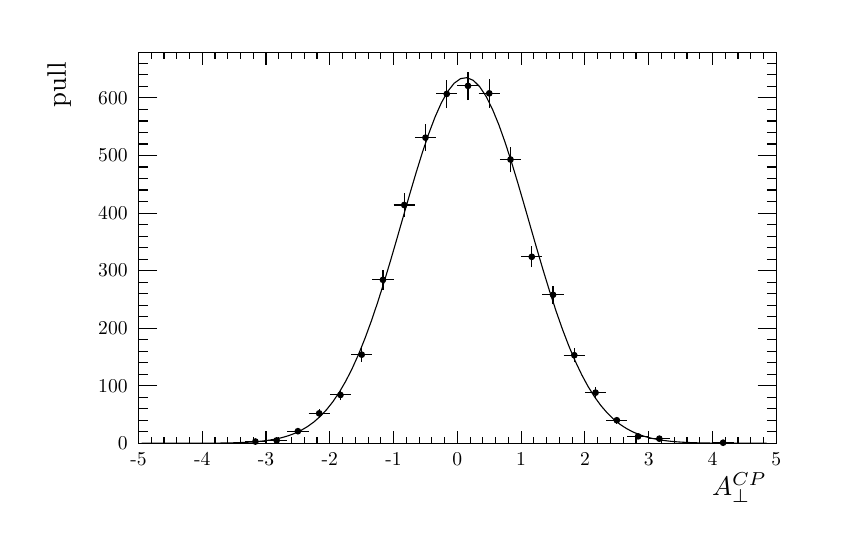
\begin{tikzpicture}
\pgfdeclareplotmark{cross} {
\pgfpathmoveto{\pgfpoint{-0.3\pgfplotmarksize}{\pgfplotmarksize}}
\pgfpathlineto{\pgfpoint{+0.3\pgfplotmarksize}{\pgfplotmarksize}}
\pgfpathlineto{\pgfpoint{+0.3\pgfplotmarksize}{0.3\pgfplotmarksize}}
\pgfpathlineto{\pgfpoint{+1\pgfplotmarksize}{0.3\pgfplotmarksize}}
\pgfpathlineto{\pgfpoint{+1\pgfplotmarksize}{-0.3\pgfplotmarksize}}
\pgfpathlineto{\pgfpoint{+0.3\pgfplotmarksize}{-0.3\pgfplotmarksize}}
\pgfpathlineto{\pgfpoint{+0.3\pgfplotmarksize}{-1.\pgfplotmarksize}}
\pgfpathlineto{\pgfpoint{-0.3\pgfplotmarksize}{-1.\pgfplotmarksize}}
\pgfpathlineto{\pgfpoint{-0.3\pgfplotmarksize}{-0.3\pgfplotmarksize}}
\pgfpathlineto{\pgfpoint{-1.\pgfplotmarksize}{-0.3\pgfplotmarksize}}
\pgfpathlineto{\pgfpoint{-1.\pgfplotmarksize}{0.3\pgfplotmarksize}}
\pgfpathlineto{\pgfpoint{-0.3\pgfplotmarksize}{0.3\pgfplotmarksize}}
\pgfpathclose
\pgfusepathqstroke
}
\pgfdeclareplotmark{cross*} {
\pgfpathmoveto{\pgfpoint{-0.3\pgfplotmarksize}{\pgfplotmarksize}}
\pgfpathlineto{\pgfpoint{+0.3\pgfplotmarksize}{\pgfplotmarksize}}
\pgfpathlineto{\pgfpoint{+0.3\pgfplotmarksize}{0.3\pgfplotmarksize}}
\pgfpathlineto{\pgfpoint{+1\pgfplotmarksize}{0.3\pgfplotmarksize}}
\pgfpathlineto{\pgfpoint{+1\pgfplotmarksize}{-0.3\pgfplotmarksize}}
\pgfpathlineto{\pgfpoint{+0.3\pgfplotmarksize}{-0.3\pgfplotmarksize}}
\pgfpathlineto{\pgfpoint{+0.3\pgfplotmarksize}{-1.\pgfplotmarksize}}
\pgfpathlineto{\pgfpoint{-0.3\pgfplotmarksize}{-1.\pgfplotmarksize}}
\pgfpathlineto{\pgfpoint{-0.3\pgfplotmarksize}{-0.3\pgfplotmarksize}}
\pgfpathlineto{\pgfpoint{-1.\pgfplotmarksize}{-0.3\pgfplotmarksize}}
\pgfpathlineto{\pgfpoint{-1.\pgfplotmarksize}{0.3\pgfplotmarksize}}
\pgfpathlineto{\pgfpoint{-0.3\pgfplotmarksize}{0.3\pgfplotmarksize}}
\pgfpathclose
\pgfusepathqfillstroke
}
\pgfdeclareplotmark{newstar} {
\pgfpathmoveto{\pgfqpoint{0pt}{\pgfplotmarksize}}
\pgfpathlineto{\pgfqpointpolar{44}{0.5\pgfplotmarksize}}
\pgfpathlineto{\pgfqpointpolar{18}{\pgfplotmarksize}}
\pgfpathlineto{\pgfqpointpolar{-20}{0.5\pgfplotmarksize}}
\pgfpathlineto{\pgfqpointpolar{-54}{\pgfplotmarksize}}
\pgfpathlineto{\pgfqpointpolar{-90}{0.5\pgfplotmarksize}}
\pgfpathlineto{\pgfqpointpolar{234}{\pgfplotmarksize}}
\pgfpathlineto{\pgfqpointpolar{198}{0.5\pgfplotmarksize}}
\pgfpathlineto{\pgfqpointpolar{162}{\pgfplotmarksize}}
\pgfpathlineto{\pgfqpointpolar{134}{0.5\pgfplotmarksize}}
\pgfpathclose
\pgfusepathqstroke
}
\pgfdeclareplotmark{newstar*} {
\pgfpathmoveto{\pgfqpoint{0pt}{\pgfplotmarksize}}
\pgfpathlineto{\pgfqpointpolar{44}{0.5\pgfplotmarksize}}
\pgfpathlineto{\pgfqpointpolar{18}{\pgfplotmarksize}}
\pgfpathlineto{\pgfqpointpolar{-20}{0.5\pgfplotmarksize}}
\pgfpathlineto{\pgfqpointpolar{-54}{\pgfplotmarksize}}
\pgfpathlineto{\pgfqpointpolar{-90}{0.5\pgfplotmarksize}}
\pgfpathlineto{\pgfqpointpolar{234}{\pgfplotmarksize}}
\pgfpathlineto{\pgfqpointpolar{198}{0.5\pgfplotmarksize}}
\pgfpathlineto{\pgfqpointpolar{162}{\pgfplotmarksize}}
\pgfpathlineto{\pgfqpointpolar{134}{0.5\pgfplotmarksize}}
\pgfpathclose
\pgfusepathqfillstroke
}
\definecolor{c}{rgb}{1,1,1};
\draw [color=c, fill=c] (0,0) rectangle (10,6.27517);
\draw [color=c, fill=c] (1.4,1.00403) rectangle (9.5,5.96141);
\definecolor{c}{rgb}{0,0,0};
\draw [c] (1.4,1.00403) -- (1.4,5.96141) -- (9.5,5.96141) -- (9.5,1.00403) -- (1.4,1.00403);
\draw [c] (2.885,1.01329) -- (2.885,1.02596);
\draw [c] (2.885,1.02596) -- (2.885,1.03862);
\draw [c] (2.75,1.02596) -- (2.885,1.02596);
\draw [c] (2.885,1.02596) -- (3.02,1.02596);
\foreach \P in {(2.885,1.02596)}{\draw[mark options={color=c,fill=c},mark size=2.402402pt,mark=*,mark size=1pt] plot coordinates {\P};}
\draw [c] (3.155,1.02423) -- (3.155,1.04057);
\draw [c] (3.155,1.04057) -- (3.155,1.05692);
\draw [c] (3.02,1.04057) -- (3.155,1.04057);
\draw [c] (3.155,1.04057) -- (3.29,1.04057);
\foreach \P in {(3.155,1.04057)}{\draw[mark options={color=c,fill=c},mark size=2.402402pt,mark=*,mark size=1pt] plot coordinates {\P};}
\draw [c] (3.425,1.12403) -- (3.425,1.15753);
\draw [c] (3.425,1.15753) -- (3.425,1.19102);
\draw [c] (3.29,1.15753) -- (3.425,1.15753);
\draw [c] (3.425,1.15753) -- (3.56,1.15753);
\foreach \P in {(3.425,1.15753)}{\draw[mark options={color=c,fill=c},mark size=2.402402pt,mark=*,mark size=1pt] plot coordinates {\P};}
\draw [c] (3.695,1.33141) -- (3.695,1.38412);
\draw [c] (3.695,1.38412) -- (3.695,1.43683);
\draw [c] (3.56,1.38412) -- (3.695,1.38412);
\draw [c] (3.695,1.38412) -- (3.83,1.38412);
\foreach \P in {(3.695,1.38412)}{\draw[mark options={color=c,fill=c},mark size=2.402402pt,mark=*,mark size=1pt] plot coordinates {\P};}
\draw [c] (3.965,1.55103) -- (3.965,1.61802);
\draw [c] (3.965,1.61802) -- (3.965,1.68501);
\draw [c] (3.83,1.61802) -- (3.965,1.61802);
\draw [c] (3.965,1.61802) -- (4.1,1.61802);
\foreach \P in {(3.965,1.61802)}{\draw[mark options={color=c,fill=c},mark size=2.402402pt,mark=*,mark size=1pt] plot coordinates {\P};}
\draw [c] (4.235,2.03897) -- (4.235,2.12968);
\draw [c] (4.235,2.12968) -- (4.235,2.22039);
\draw [c] (4.1,2.12968) -- (4.235,2.12968);
\draw [c] (4.235,2.12968) -- (4.37,2.12968);
\foreach \P in {(4.235,2.12968)}{\draw[mark options={color=c,fill=c},mark size=2.402402pt,mark=*,mark size=1pt] plot coordinates {\P};}
\draw [c] (4.505,2.95673) -- (4.505,3.07991);
\draw [c] (4.505,3.07991) -- (4.505,3.20309);
\draw [c] (4.37,3.07991) -- (4.505,3.07991);
\draw [c] (4.505,3.07991) -- (4.64,3.07991);
\foreach \P in {(4.505,3.07991)}{\draw[mark options={color=c,fill=c},mark size=2.402402pt,mark=*,mark size=1pt] plot coordinates {\P};}
\draw [c] (4.775,3.88141) -- (4.775,4.03014);
\draw [c] (4.775,4.03014) -- (4.775,4.17886);
\draw [c] (4.64,4.03014) -- (4.775,4.03014);
\draw [c] (4.775,4.03014) -- (4.91,4.03014);
\foreach \P in {(4.775,4.03014)}{\draw[mark options={color=c,fill=c},mark size=2.402402pt,mark=*,mark size=1pt] plot coordinates {\P};}
\draw [c] (5.045,4.71691) -- (5.045,4.88534);
\draw [c] (5.045,4.88534) -- (5.045,5.05378);
\draw [c] (4.91,4.88534) -- (5.045,4.88534);
\draw [c] (5.045,4.88534) -- (5.18,4.88534);
\foreach \P in {(5.045,4.88534)}{\draw[mark options={color=c,fill=c},mark size=2.402402pt,mark=*,mark size=1pt] plot coordinates {\P};}
\draw [c] (5.315,5.26078) -- (5.315,5.44086);
\draw [c] (5.315,5.44086) -- (5.315,5.62095);
\draw [c] (5.18,5.44086) -- (5.315,5.44086);
\draw [c] (5.315,5.44086) -- (5.45,5.44086);
\foreach \P in {(5.315,5.44086)}{\draw[mark options={color=c,fill=c},mark size=2.402402pt,mark=*,mark size=1pt] plot coordinates {\P};}
\draw [c] (5.585,5.36104) -- (5.585,5.54319);
\draw [c] (5.585,5.54319) -- (5.585,5.72534);
\draw [c] (5.45,5.54319) -- (5.585,5.54319);
\draw [c] (5.585,5.54319) -- (5.72,5.54319);
\foreach \P in {(5.585,5.54319)}{\draw[mark options={color=c,fill=c},mark size=2.402402pt,mark=*,mark size=1pt] plot coordinates {\P};}
\draw [c] (5.855,5.26794) -- (5.855,5.44817);
\draw [c] (5.855,5.44817) -- (5.855,5.6284);
\draw [c] (5.72,5.44817) -- (5.855,5.44817);
\draw [c] (5.855,5.44817) -- (5.99,5.44817);
\foreach \P in {(5.855,5.44817)}{\draw[mark options={color=c,fill=c},mark size=2.402402pt,mark=*,mark size=1pt] plot coordinates {\P};}
\draw [c] (6.125,4.44529) -- (6.125,4.60758);
\draw [c] (6.125,4.60758) -- (6.125,4.76988);
\draw [c] (5.99,4.60758) -- (6.125,4.60758);
\draw [c] (6.125,4.60758) -- (6.26,4.60758);
\foreach \P in {(6.125,4.60758)}{\draw[mark options={color=c,fill=c},mark size=2.402402pt,mark=*,mark size=1pt] plot coordinates {\P};}
\draw [c] (6.395,3.24072) -- (6.395,3.37229);
\draw [c] (6.395,3.37229) -- (6.395,3.50386);
\draw [c] (6.26,3.37229) -- (6.395,3.37229);
\draw [c] (6.395,3.37229) -- (6.53,3.37229);
\foreach \P in {(6.395,3.37229)}{\draw[mark options={color=c,fill=c},mark size=2.402402pt,mark=*,mark size=1pt] plot coordinates {\P};}
\draw [c] (6.665,2.77246) -- (6.665,2.88986);
\draw [c] (6.665,2.88986) -- (6.665,3.00727);
\draw [c] (6.53,2.88986) -- (6.665,2.88986);
\draw [c] (6.665,2.88986) -- (6.8,2.88986);
\foreach \P in {(6.665,2.88986)}{\draw[mark options={color=c,fill=c},mark size=2.402402pt,mark=*,mark size=1pt] plot coordinates {\P};}
\draw [c] (6.935,2.03196) -- (6.935,2.12237);
\draw [c] (6.935,2.12237) -- (6.935,2.21279);
\draw [c] (6.8,2.12237) -- (6.935,2.12237);
\draw [c] (6.935,2.12237) -- (7.07,2.12237);
\foreach \P in {(6.935,2.12237)}{\draw[mark options={color=c,fill=c},mark size=2.402402pt,mark=*,mark size=1pt] plot coordinates {\P};}
\draw [c] (7.205,1.57869) -- (7.205,1.64726);
\draw [c] (7.205,1.64726) -- (7.205,1.71583);
\draw [c] (7.07,1.64726) -- (7.205,1.64726);
\draw [c] (7.205,1.64726) -- (7.34,1.64726);
\foreach \P in {(7.205,1.64726)}{\draw[mark options={color=c,fill=c},mark size=2.402402pt,mark=*,mark size=1pt] plot coordinates {\P};}
\draw [c] (7.475,1.25018) -- (7.475,1.2964);
\draw [c] (7.475,1.2964) -- (7.475,1.34263);
\draw [c] (7.34,1.2964) -- (7.475,1.2964);
\draw [c] (7.475,1.2964) -- (7.61,1.2964);
\foreach \P in {(7.475,1.2964)}{\draw[mark options={color=c,fill=c},mark size=2.402402pt,mark=*,mark size=1pt] plot coordinates {\P};}
\draw [c] (7.745,1.06642) -- (7.745,1.09174);
\draw [c] (7.745,1.09174) -- (7.745,1.11706);
\draw [c] (7.61,1.09174) -- (7.745,1.09174);
\draw [c] (7.745,1.09174) -- (7.88,1.09174);
\foreach \P in {(7.745,1.09174)}{\draw[mark options={color=c,fill=c},mark size=2.402402pt,mark=*,mark size=1pt] plot coordinates {\P};}
\draw [c] (8.015,1.04183) -- (8.015,1.0625);
\draw [c] (8.015,1.0625) -- (8.015,1.08318);
\draw [c] (7.88,1.0625) -- (8.015,1.0625);
\draw [c] (8.015,1.0625) -- (8.15,1.0625);
\foreach \P in {(8.015,1.0625)}{\draw[mark options={color=c,fill=c},mark size=2.402402pt,mark=*,mark size=1pt] plot coordinates {\P};}
\draw [c] (8.825,1.00403) -- (8.825,1.01134);
\draw [c] (8.825,1.01134) -- (8.825,1.01865);
\draw [c] (8.69,1.01134) -- (8.825,1.01134);
\draw [c] (8.825,1.01134) -- (8.96,1.01134);
\foreach \P in {(8.825,1.01134)}{\draw[mark options={color=c,fill=c},mark size=2.402402pt,mark=*,mark size=1pt] plot coordinates {\P};}
\draw [c,line width=0.4] (1.4405,1.00403) -- (1.5215,1.00403) -- (1.6025,1.00403) -- (1.6835,1.00403) -- (1.7645,1.00403) -- (1.8455,1.00403) -- (1.9265,1.00403) -- (2.0075,1.00403) -- (2.0885,1.00403) -- (2.1695,1.00474) -- (2.2505,1.0051) --
 (2.3315,1.00564) -- (2.4125,1.00643) -- (2.4935,1.00756) -- (2.5745,1.00917) -- (2.6555,1.01143) -- (2.7365,1.01459) -- (2.8175,1.01894) -- (2.8985,1.02488) -- (2.9795,1.03289) -- (3.0605,1.04357) -- (3.1415,1.05766) -- (3.2225,1.07604) --
 (3.3035,1.09976) -- (3.3845,1.13002) -- (3.4655,1.16817) -- (3.5465,1.21573) -- (3.6275,1.27434) -- (3.7085,1.34572) -- (3.7895,1.43161) -- (3.8705,1.53374) -- (3.9515,1.65367) -- (4.0325,1.79278) -- (4.1135,1.95208) -- (4.1945,2.13213) --
 (4.2755,2.33292) -- (4.3565,2.55377) -- (4.4375,2.79319) -- (4.5185,3.04891) -- (4.5995,3.31776) -- (4.6805,3.59571) -- (4.7615,3.87796) -- (4.8425,4.159) -- (4.9235,4.43282) -- (5.0045,4.69306) -- (5.0855,4.93327) -- (5.1665,5.14717) --
 (5.2475,5.32894) -- (5.3285,5.47344) -- (5.4095,5.57647);
\draw [c,line width=0.4] (5.4095,5.57647) -- (5.4905,5.635) -- (5.5715,5.64727) -- (5.6525,5.61292) -- (5.7335,5.53297) -- (5.8145,5.4098) -- (5.8955,5.24703) -- (5.9765,5.04932) -- (6.0575,4.82217) -- (6.1385,4.57165) -- (6.2195,4.30417) --
 (6.3005,4.02614) -- (6.3815,3.7438) -- (6.4625,3.46295) -- (6.5435,3.18877) -- (6.6245,2.9257) -- (6.7055,2.67737) -- (6.7865,2.44653) -- (6.8675,2.23507) -- (6.9485,2.04408) -- (7.0295,1.87392) -- (7.1105,1.7243) -- (7.1915,1.59444) --
 (7.2725,1.48314) -- (7.3535,1.38893) -- (7.4345,1.31014) -- (7.5155,1.24504) -- (7.5965,1.19189) -- (7.6775,1.14899) -- (7.7585,1.11476) -- (7.8395,1.08777) -- (7.9205,1.06672) -- (8.0015,1.05049) -- (8.0825,1.03812) -- (8.1635,1.02879) --
 (8.2445,1.02184) -- (8.3255,1.0167) -- (8.4065,1.01296) -- (8.4875,1.01026) -- (8.5685,1.00833) -- (8.6495,1.00697) -- (8.7305,1.00602) -- (8.8115,1.00536) -- (8.8925,1.00491) -- (8.9735,1.00461) -- (9.0545,1.00403) -- (9.1355,1.00403) --
 (9.2165,1.00403) -- (9.2975,1.00403) -- (9.3785,1.00403);
\draw [c,line width=0.4] (9.3785,1.00403) -- (9.4595,1.00403);
\draw [c,line width=0.4] (1.4,1.00403) -- (9.5,1.00403);
\draw [anchor= east] (9.5,0.441772) node[scale=0.96888, rotate=0]{$A^{CP}_{\perp}$};
\draw [c,line width=0.4] (1.4,1.15651) -- (1.4,1.00403);
\draw [c,line width=0.4] (1.562,1.08027) -- (1.562,1.00403);
\draw [c,line width=0.4] (1.724,1.08027) -- (1.724,1.00403);
\draw [c,line width=0.4] (1.886,1.08027) -- (1.886,1.00403);
\draw [c,line width=0.4] (2.048,1.08027) -- (2.048,1.00403);
\draw [c,line width=0.4] (2.21,1.15651) -- (2.21,1.00403);
\draw [c,line width=0.4] (2.372,1.08027) -- (2.372,1.00403);
\draw [c,line width=0.4] (2.534,1.08027) -- (2.534,1.00403);
\draw [c,line width=0.4] (2.696,1.08027) -- (2.696,1.00403);
\draw [c,line width=0.4] (2.858,1.08027) -- (2.858,1.00403);
\draw [c,line width=0.4] (3.02,1.15651) -- (3.02,1.00403);
\draw [c,line width=0.4] (3.182,1.08027) -- (3.182,1.00403);
\draw [c,line width=0.4] (3.344,1.08027) -- (3.344,1.00403);
\draw [c,line width=0.4] (3.506,1.08027) -- (3.506,1.00403);
\draw [c,line width=0.4] (3.668,1.08027) -- (3.668,1.00403);
\draw [c,line width=0.4] (3.83,1.15651) -- (3.83,1.00403);
\draw [c,line width=0.4] (3.992,1.08027) -- (3.992,1.00403);
\draw [c,line width=0.4] (4.154,1.08027) -- (4.154,1.00403);
\draw [c,line width=0.4] (4.316,1.08027) -- (4.316,1.00403);
\draw [c,line width=0.4] (4.478,1.08027) -- (4.478,1.00403);
\draw [c,line width=0.4] (4.64,1.15651) -- (4.64,1.00403);
\draw [c,line width=0.4] (4.802,1.08027) -- (4.802,1.00403);
\draw [c,line width=0.4] (4.964,1.08027) -- (4.964,1.00403);
\draw [c,line width=0.4] (5.126,1.08027) -- (5.126,1.00403);
\draw [c,line width=0.4] (5.288,1.08027) -- (5.288,1.00403);
\draw [c,line width=0.4] (5.45,1.15651) -- (5.45,1.00403);
\draw [c,line width=0.4] (5.612,1.08027) -- (5.612,1.00403);
\draw [c,line width=0.4] (5.774,1.08027) -- (5.774,1.00403);
\draw [c,line width=0.4] (5.936,1.08027) -- (5.936,1.00403);
\draw [c,line width=0.4] (6.098,1.08027) -- (6.098,1.00403);
\draw [c,line width=0.4] (6.26,1.15651) -- (6.26,1.00403);
\draw [c,line width=0.4] (6.422,1.08027) -- (6.422,1.00403);
\draw [c,line width=0.4] (6.584,1.08027) -- (6.584,1.00403);
\draw [c,line width=0.4] (6.746,1.08027) -- (6.746,1.00403);
\draw [c,line width=0.4] (6.908,1.08027) -- (6.908,1.00403);
\draw [c,line width=0.4] (7.07,1.15651) -- (7.07,1.00403);
\draw [c,line width=0.4] (7.232,1.08027) -- (7.232,1.00403);
\draw [c,line width=0.4] (7.394,1.08027) -- (7.394,1.00403);
\draw [c,line width=0.4] (7.556,1.08027) -- (7.556,1.00403);
\draw [c,line width=0.4] (7.718,1.08027) -- (7.718,1.00403);
\draw [c,line width=0.4] (7.88,1.15651) -- (7.88,1.00403);
\draw [c,line width=0.4] (8.042,1.08027) -- (8.042,1.00403);
\draw [c,line width=0.4] (8.204,1.08027) -- (8.204,1.00403);
\draw [c,line width=0.4] (8.366,1.08027) -- (8.366,1.00403);
\draw [c,line width=0.4] (8.528,1.08027) -- (8.528,1.00403);
\draw [c,line width=0.4] (8.69,1.15651) -- (8.69,1.00403);
\draw [c,line width=0.4] (8.852,1.08027) -- (8.852,1.00403);
\draw [c,line width=0.4] (9.014,1.08027) -- (9.014,1.00403);
\draw [c,line width=0.4] (9.176,1.08027) -- (9.176,1.00403);
\draw [c,line width=0.4] (9.338,1.08027) -- (9.338,1.00403);
\draw [c,line width=0.4] (9.5,1.15651) -- (9.5,1.00403);
\draw [anchor=base] (1.4,0.721644) node[scale=0.708027, rotate=0]{-5};
\draw [anchor=base] (2.21,0.721644) node[scale=0.708027, rotate=0]{-4};
\draw [anchor=base] (3.02,0.721644) node[scale=0.708027, rotate=0]{-3};
\draw [anchor=base] (3.83,0.721644) node[scale=0.708027, rotate=0]{-2};
\draw [anchor=base] (4.64,0.721644) node[scale=0.708027, rotate=0]{-1};
\draw [anchor=base] (5.45,0.721644) node[scale=0.708027, rotate=0]{0};
\draw [anchor=base] (6.26,0.721644) node[scale=0.708027, rotate=0]{1};
\draw [anchor=base] (7.07,0.721644) node[scale=0.708027, rotate=0]{2};
\draw [anchor=base] (7.88,0.721644) node[scale=0.708027, rotate=0]{3};
\draw [anchor=base] (8.69,0.721644) node[scale=0.708027, rotate=0]{4};
\draw [anchor=base] (9.5,0.721644) node[scale=0.708027, rotate=0]{5};
\draw [c,line width=0.4] (1.4,5.96141) -- (9.5,5.96141);
\draw [c,line width=0.4] (1.4,5.80892) -- (1.4,5.96141);
\draw [c,line width=0.4] (1.562,5.88517) -- (1.562,5.96141);
\draw [c,line width=0.4] (1.724,5.88517) -- (1.724,5.96141);
\draw [c,line width=0.4] (1.886,5.88517) -- (1.886,5.96141);
\draw [c,line width=0.4] (2.048,5.88517) -- (2.048,5.96141);
\draw [c,line width=0.4] (2.21,5.80892) -- (2.21,5.96141);
\draw [c,line width=0.4] (2.372,5.88517) -- (2.372,5.96141);
\draw [c,line width=0.4] (2.534,5.88517) -- (2.534,5.96141);
\draw [c,line width=0.4] (2.696,5.88517) -- (2.696,5.96141);
\draw [c,line width=0.4] (2.858,5.88517) -- (2.858,5.96141);
\draw [c,line width=0.4] (3.02,5.80892) -- (3.02,5.96141);
\draw [c,line width=0.4] (3.182,5.88517) -- (3.182,5.96141);
\draw [c,line width=0.4] (3.344,5.88517) -- (3.344,5.96141);
\draw [c,line width=0.4] (3.506,5.88517) -- (3.506,5.96141);
\draw [c,line width=0.4] (3.668,5.88517) -- (3.668,5.96141);
\draw [c,line width=0.4] (3.83,5.80892) -- (3.83,5.96141);
\draw [c,line width=0.4] (3.992,5.88517) -- (3.992,5.96141);
\draw [c,line width=0.4] (4.154,5.88517) -- (4.154,5.96141);
\draw [c,line width=0.4] (4.316,5.88517) -- (4.316,5.96141);
\draw [c,line width=0.4] (4.478,5.88517) -- (4.478,5.96141);
\draw [c,line width=0.4] (4.64,5.80892) -- (4.64,5.96141);
\draw [c,line width=0.4] (4.802,5.88517) -- (4.802,5.96141);
\draw [c,line width=0.4] (4.964,5.88517) -- (4.964,5.96141);
\draw [c,line width=0.4] (5.126,5.88517) -- (5.126,5.96141);
\draw [c,line width=0.4] (5.288,5.88517) -- (5.288,5.96141);
\draw [c,line width=0.4] (5.45,5.80892) -- (5.45,5.96141);
\draw [c,line width=0.4] (5.612,5.88517) -- (5.612,5.96141);
\draw [c,line width=0.4] (5.774,5.88517) -- (5.774,5.96141);
\draw [c,line width=0.4] (5.936,5.88517) -- (5.936,5.96141);
\draw [c,line width=0.4] (6.098,5.88517) -- (6.098,5.96141);
\draw [c,line width=0.4] (6.26,5.80892) -- (6.26,5.96141);
\draw [c,line width=0.4] (6.422,5.88517) -- (6.422,5.96141);
\draw [c,line width=0.4] (6.584,5.88517) -- (6.584,5.96141);
\draw [c,line width=0.4] (6.746,5.88517) -- (6.746,5.96141);
\draw [c,line width=0.4] (6.908,5.88517) -- (6.908,5.96141);
\draw [c,line width=0.4] (7.07,5.80892) -- (7.07,5.96141);
\draw [c,line width=0.4] (7.232,5.88517) -- (7.232,5.96141);
\draw [c,line width=0.4] (7.394,5.88517) -- (7.394,5.96141);
\draw [c,line width=0.4] (7.556,5.88517) -- (7.556,5.96141);
\draw [c,line width=0.4] (7.718,5.88517) -- (7.718,5.96141);
\draw [c,line width=0.4] (7.88,5.80892) -- (7.88,5.96141);
\draw [c,line width=0.4] (8.042,5.88517) -- (8.042,5.96141);
\draw [c,line width=0.4] (8.204,5.88517) -- (8.204,5.96141);
\draw [c,line width=0.4] (8.366,5.88517) -- (8.366,5.96141);
\draw [c,line width=0.4] (8.528,5.88517) -- (8.528,5.96141);
\draw [c,line width=0.4] (8.69,5.80892) -- (8.69,5.96141);
\draw [c,line width=0.4] (8.852,5.88517) -- (8.852,5.96141);
\draw [c,line width=0.4] (9.014,5.88517) -- (9.014,5.96141);
\draw [c,line width=0.4] (9.176,5.88517) -- (9.176,5.96141);
\draw [c,line width=0.4] (9.338,5.88517) -- (9.338,5.96141);
\draw [c,line width=0.4] (9.5,5.80892) -- (9.5,5.96141);
\draw [c,line width=0.4] (1.4,1.00403) -- (1.4,5.96141);
\draw [anchor= east] (0.392,5.96141) node[scale=0.96888, rotate=90]{pull};
\draw [c,line width=0.4] (1.637,1.00403) -- (1.4,1.00403);
\draw [c,line width=0.4] (1.5185,1.15022) -- (1.4,1.15022);
\draw [c,line width=0.4] (1.5185,1.2964) -- (1.4,1.2964);
\draw [c,line width=0.4] (1.5185,1.44259) -- (1.4,1.44259);
\draw [c,line width=0.4] (1.5185,1.58878) -- (1.4,1.58878);
\draw [c,line width=0.4] (1.637,1.73497) -- (1.4,1.73497);
\draw [c,line width=0.4] (1.5185,1.88116) -- (1.4,1.88116);
\draw [c,line width=0.4] (1.5185,2.02735) -- (1.4,2.02735);
\draw [c,line width=0.4] (1.5185,2.17354) -- (1.4,2.17354);
\draw [c,line width=0.4] (1.5185,2.31973) -- (1.4,2.31973);
\draw [c,line width=0.4] (1.637,2.46592) -- (1.4,2.46592);
\draw [c,line width=0.4] (1.5185,2.61211) -- (1.4,2.61211);
\draw [c,line width=0.4] (1.5185,2.75829) -- (1.4,2.75829);
\draw [c,line width=0.4] (1.5185,2.90448) -- (1.4,2.90448);
\draw [c,line width=0.4] (1.5185,3.05067) -- (1.4,3.05067);
\draw [c,line width=0.4] (1.637,3.19686) -- (1.4,3.19686);
\draw [c,line width=0.4] (1.5185,3.34305) -- (1.4,3.34305);
\draw [c,line width=0.4] (1.5185,3.48924) -- (1.4,3.48924);
\draw [c,line width=0.4] (1.5185,3.63543) -- (1.4,3.63543);
\draw [c,line width=0.4] (1.5185,3.78162) -- (1.4,3.78162);
\draw [c,line width=0.4] (1.637,3.92781) -- (1.4,3.92781);
\draw [c,line width=0.4] (1.5185,4.07399) -- (1.4,4.07399);
\draw [c,line width=0.4] (1.5185,4.22018) -- (1.4,4.22018);
\draw [c,line width=0.4] (1.5185,4.36637) -- (1.4,4.36637);
\draw [c,line width=0.4] (1.5185,4.51256) -- (1.4,4.51256);
\draw [c,line width=0.4] (1.637,4.65875) -- (1.4,4.65875);
\draw [c,line width=0.4] (1.5185,4.80494) -- (1.4,4.80494);
\draw [c,line width=0.4] (1.5185,4.95113) -- (1.4,4.95113);
\draw [c,line width=0.4] (1.5185,5.09732) -- (1.4,5.09732);
\draw [c,line width=0.4] (1.5185,5.24351) -- (1.4,5.24351);
\draw [c,line width=0.4] (1.637,5.38969) -- (1.4,5.38969);
\draw [c,line width=0.4] (1.637,5.38969) -- (1.4,5.38969);
\draw [c,line width=0.4] (1.5185,5.53588) -- (1.4,5.53588);
\draw [c,line width=0.4] (1.5185,5.68207) -- (1.4,5.68207);
\draw [c,line width=0.4] (1.5185,5.82826) -- (1.4,5.82826);
\draw [anchor= east] (1.35,1.00403) node[scale=0.708027, rotate=0]{0};
\draw [anchor= east] (1.35,1.73497) node[scale=0.708027, rotate=0]{100};
\draw [anchor= east] (1.35,2.46592) node[scale=0.708027, rotate=0]{200};
\draw [anchor= east] (1.35,3.19686) node[scale=0.708027, rotate=0]{300};
\draw [anchor= east] (1.35,3.92781) node[scale=0.708027, rotate=0]{400};
\draw [anchor= east] (1.35,4.65875) node[scale=0.708027, rotate=0]{500};
\draw [anchor= east] (1.35,5.38969) node[scale=0.708027, rotate=0]{600};
\draw [c,line width=0.4] (9.5,1.00403) -- (9.5,5.96141);
\draw [c,line width=0.4] (9.263,1.00403) -- (9.5,1.00403);
\draw [c,line width=0.4] (9.3815,1.15022) -- (9.5,1.15022);
\draw [c,line width=0.4] (9.3815,1.2964) -- (9.5,1.2964);
\draw [c,line width=0.4] (9.3815,1.44259) -- (9.5,1.44259);
\draw [c,line width=0.4] (9.3815,1.58878) -- (9.5,1.58878);
\draw [c,line width=0.4] (9.263,1.73497) -- (9.5,1.73497);
\draw [c,line width=0.4] (9.3815,1.88116) -- (9.5,1.88116);
\draw [c,line width=0.4] (9.3815,2.02735) -- (9.5,2.02735);
\draw [c,line width=0.4] (9.3815,2.17354) -- (9.5,2.17354);
\draw [c,line width=0.4] (9.3815,2.31973) -- (9.5,2.31973);
\draw [c,line width=0.4] (9.263,2.46592) -- (9.5,2.46592);
\draw [c,line width=0.4] (9.3815,2.61211) -- (9.5,2.61211);
\draw [c,line width=0.4] (9.3815,2.75829) -- (9.5,2.75829);
\draw [c,line width=0.4] (9.3815,2.90448) -- (9.5,2.90448);
\draw [c,line width=0.4] (9.3815,3.05067) -- (9.5,3.05067);
\draw [c,line width=0.4] (9.263,3.19686) -- (9.5,3.19686);
\draw [c,line width=0.4] (9.3815,3.34305) -- (9.5,3.34305);
\draw [c,line width=0.4] (9.3815,3.48924) -- (9.5,3.48924);
\draw [c,line width=0.4] (9.3815,3.63543) -- (9.5,3.63543);
\draw [c,line width=0.4] (9.3815,3.78162) -- (9.5,3.78162);
\draw [c,line width=0.4] (9.263,3.92781) -- (9.5,3.92781);
\draw [c,line width=0.4] (9.3815,4.07399) -- (9.5,4.07399);
\draw [c,line width=0.4] (9.3815,4.22018) -- (9.5,4.22018);
\draw [c,line width=0.4] (9.3815,4.36637) -- (9.5,4.36637);
\draw [c,line width=0.4] (9.3815,4.51256) -- (9.5,4.51256);
\draw [c,line width=0.4] (9.263,4.65875) -- (9.5,4.65875);
\draw [c,line width=0.4] (9.3815,4.80494) -- (9.5,4.80494);
\draw [c,line width=0.4] (9.3815,4.95113) -- (9.5,4.95113);
\draw [c,line width=0.4] (9.3815,5.09732) -- (9.5,5.09732);
\draw [c,line width=0.4] (9.3815,5.24351) -- (9.5,5.24351);
\draw [c,line width=0.4] (9.263,5.38969) -- (9.5,5.38969);
\draw [c,line width=0.4] (9.263,5.38969) -- (9.5,5.38969);
\draw [c,line width=0.4] (9.3815,5.53588) -- (9.5,5.53588);
\draw [c,line width=0.4] (9.3815,5.68207) -- (9.5,5.68207);
\draw [c,line width=0.4] (9.3815,5.82826) -- (9.5,5.82826);
\end{tikzpicture}
}
    \caption{}
    \label{pull_ACPperp}
  \end{subfigure}
  \begin{subfigure}{0.5\textwidth}
    \tikzsetnextfilename{pull_ACPpar} 
    \scalebox{0.60}{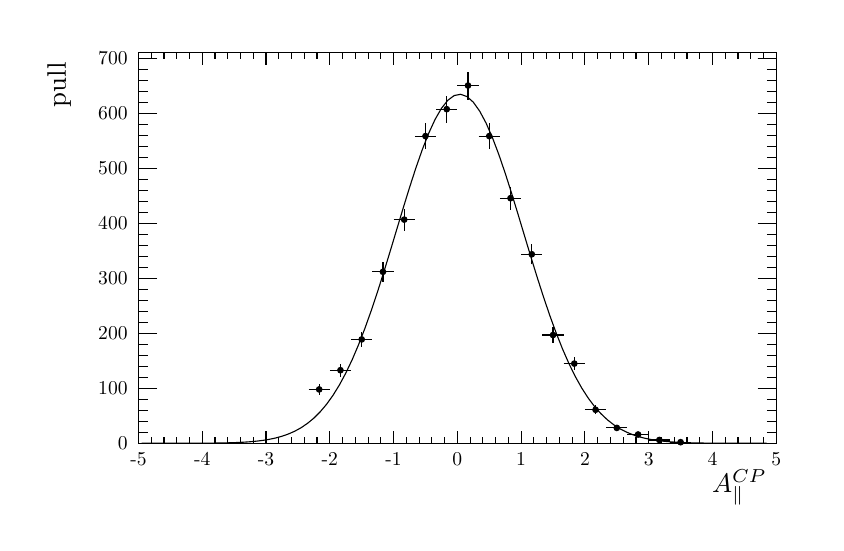
\begin{tikzpicture}
\pgfdeclareplotmark{cross} {
\pgfpathmoveto{\pgfpoint{-0.3\pgfplotmarksize}{\pgfplotmarksize}}
\pgfpathlineto{\pgfpoint{+0.3\pgfplotmarksize}{\pgfplotmarksize}}
\pgfpathlineto{\pgfpoint{+0.3\pgfplotmarksize}{0.3\pgfplotmarksize}}
\pgfpathlineto{\pgfpoint{+1\pgfplotmarksize}{0.3\pgfplotmarksize}}
\pgfpathlineto{\pgfpoint{+1\pgfplotmarksize}{-0.3\pgfplotmarksize}}
\pgfpathlineto{\pgfpoint{+0.3\pgfplotmarksize}{-0.3\pgfplotmarksize}}
\pgfpathlineto{\pgfpoint{+0.3\pgfplotmarksize}{-1.\pgfplotmarksize}}
\pgfpathlineto{\pgfpoint{-0.3\pgfplotmarksize}{-1.\pgfplotmarksize}}
\pgfpathlineto{\pgfpoint{-0.3\pgfplotmarksize}{-0.3\pgfplotmarksize}}
\pgfpathlineto{\pgfpoint{-1.\pgfplotmarksize}{-0.3\pgfplotmarksize}}
\pgfpathlineto{\pgfpoint{-1.\pgfplotmarksize}{0.3\pgfplotmarksize}}
\pgfpathlineto{\pgfpoint{-0.3\pgfplotmarksize}{0.3\pgfplotmarksize}}
\pgfpathclose
\pgfusepathqstroke
}
\pgfdeclareplotmark{cross*} {
\pgfpathmoveto{\pgfpoint{-0.3\pgfplotmarksize}{\pgfplotmarksize}}
\pgfpathlineto{\pgfpoint{+0.3\pgfplotmarksize}{\pgfplotmarksize}}
\pgfpathlineto{\pgfpoint{+0.3\pgfplotmarksize}{0.3\pgfplotmarksize}}
\pgfpathlineto{\pgfpoint{+1\pgfplotmarksize}{0.3\pgfplotmarksize}}
\pgfpathlineto{\pgfpoint{+1\pgfplotmarksize}{-0.3\pgfplotmarksize}}
\pgfpathlineto{\pgfpoint{+0.3\pgfplotmarksize}{-0.3\pgfplotmarksize}}
\pgfpathlineto{\pgfpoint{+0.3\pgfplotmarksize}{-1.\pgfplotmarksize}}
\pgfpathlineto{\pgfpoint{-0.3\pgfplotmarksize}{-1.\pgfplotmarksize}}
\pgfpathlineto{\pgfpoint{-0.3\pgfplotmarksize}{-0.3\pgfplotmarksize}}
\pgfpathlineto{\pgfpoint{-1.\pgfplotmarksize}{-0.3\pgfplotmarksize}}
\pgfpathlineto{\pgfpoint{-1.\pgfplotmarksize}{0.3\pgfplotmarksize}}
\pgfpathlineto{\pgfpoint{-0.3\pgfplotmarksize}{0.3\pgfplotmarksize}}
\pgfpathclose
\pgfusepathqfillstroke
}
\pgfdeclareplotmark{newstar} {
\pgfpathmoveto{\pgfqpoint{0pt}{\pgfplotmarksize}}
\pgfpathlineto{\pgfqpointpolar{44}{0.5\pgfplotmarksize}}
\pgfpathlineto{\pgfqpointpolar{18}{\pgfplotmarksize}}
\pgfpathlineto{\pgfqpointpolar{-20}{0.5\pgfplotmarksize}}
\pgfpathlineto{\pgfqpointpolar{-54}{\pgfplotmarksize}}
\pgfpathlineto{\pgfqpointpolar{-90}{0.5\pgfplotmarksize}}
\pgfpathlineto{\pgfqpointpolar{234}{\pgfplotmarksize}}
\pgfpathlineto{\pgfqpointpolar{198}{0.5\pgfplotmarksize}}
\pgfpathlineto{\pgfqpointpolar{162}{\pgfplotmarksize}}
\pgfpathlineto{\pgfqpointpolar{134}{0.5\pgfplotmarksize}}
\pgfpathclose
\pgfusepathqstroke
}
\pgfdeclareplotmark{newstar*} {
\pgfpathmoveto{\pgfqpoint{0pt}{\pgfplotmarksize}}
\pgfpathlineto{\pgfqpointpolar{44}{0.5\pgfplotmarksize}}
\pgfpathlineto{\pgfqpointpolar{18}{\pgfplotmarksize}}
\pgfpathlineto{\pgfqpointpolar{-20}{0.5\pgfplotmarksize}}
\pgfpathlineto{\pgfqpointpolar{-54}{\pgfplotmarksize}}
\pgfpathlineto{\pgfqpointpolar{-90}{0.5\pgfplotmarksize}}
\pgfpathlineto{\pgfqpointpolar{234}{\pgfplotmarksize}}
\pgfpathlineto{\pgfqpointpolar{198}{0.5\pgfplotmarksize}}
\pgfpathlineto{\pgfqpointpolar{162}{\pgfplotmarksize}}
\pgfpathlineto{\pgfqpointpolar{134}{0.5\pgfplotmarksize}}
\pgfpathclose
\pgfusepathqfillstroke
}
\definecolor{c}{rgb}{1,1,1};
\draw [color=c, fill=c] (0,0) rectangle (10,6.27517);
\draw [color=c, fill=c] (1.4,1.00403) rectangle (9.5,5.96141);
\definecolor{c}{rgb}{0,0,0};
\draw [c] (1.4,1.00403) -- (1.4,5.96141) -- (9.5,5.96141) -- (9.5,1.00403) -- (1.4,1.00403);
\draw [c] (3.695,1.61887) -- (3.695,1.68796);
\draw [c] (3.695,1.68796) -- (3.695,1.75704);
\draw [c] (3.56,1.68796) -- (3.695,1.68796);
\draw [c] (3.695,1.68796) -- (3.83,1.68796);
\foreach \P in {(3.695,1.68796)}{\draw[mark options={color=c,fill=c},mark size=2.402402pt,mark=*,mark size=1pt] plot coordinates {\P};}
\draw [c] (3.965,1.85173) -- (3.965,1.93222);
\draw [c] (3.965,1.93222) -- (3.965,2.0127);
\draw [c] (3.83,1.93222) -- (3.965,1.93222);
\draw [c] (3.965,1.93222) -- (4.1,1.93222);
\foreach \P in {(3.965,1.93222)}{\draw[mark options={color=c,fill=c},mark size=2.402402pt,mark=*,mark size=1pt] plot coordinates {\P};}
\draw [c] (4.235,2.22709) -- (4.235,2.32304);
\draw [c] (4.235,2.32304) -- (4.235,2.41898);
\draw [c] (4.1,2.32304) -- (4.235,2.32304);
\draw [c] (4.235,2.32304) -- (4.37,2.32304);
\foreach \P in {(4.235,2.32304)}{\draw[mark options={color=c,fill=c},mark size=2.402402pt,mark=*,mark size=1pt] plot coordinates {\P};}
\draw [c] (4.505,3.05817) -- (4.505,3.18144);
\draw [c] (4.505,3.18144) -- (4.505,3.30471);
\draw [c] (4.37,3.18144) -- (4.505,3.18144);
\draw [c] (4.505,3.18144) -- (4.64,3.18144);
\foreach \P in {(4.505,3.18144)}{\draw[mark options={color=c,fill=c},mark size=2.402402pt,mark=*,mark size=1pt] plot coordinates {\P};}
\draw [c] (4.775,3.70364) -- (4.775,3.84443);
\draw [c] (4.775,3.84443) -- (4.775,3.98523);
\draw [c] (4.64,3.84443) -- (4.775,3.84443);
\draw [c] (4.775,3.84443) -- (4.91,3.84443);
\foreach \P in {(4.775,3.84443)}{\draw[mark options={color=c,fill=c},mark size=2.402402pt,mark=*,mark size=1pt] plot coordinates {\P};}
\draw [c] (5.045,4.74022) -- (5.045,4.90522);
\draw [c] (5.045,4.90522) -- (5.045,5.07023);
\draw [c] (4.91,4.90522) -- (5.045,4.90522);
\draw [c] (5.045,4.90522) -- (5.18,4.90522);
\foreach \P in {(5.045,4.90522)}{\draw[mark options={color=c,fill=c},mark size=2.402402pt,mark=*,mark size=1pt] plot coordinates {\P};}
\draw [c] (5.315,5.0751) -- (5.315,5.24719);
\draw [c] (5.315,5.24719) -- (5.315,5.41927);
\draw [c] (5.18,5.24719) -- (5.315,5.24719);
\draw [c] (5.315,5.24719) -- (5.45,5.24719);
\foreach \P in {(5.315,5.24719)}{\draw[mark options={color=c,fill=c},mark size=2.402402pt,mark=*,mark size=1pt] plot coordinates {\P};}
\draw [c] (5.585,5.36922) -- (5.585,5.54728);
\draw [c] (5.585,5.54728) -- (5.585,5.72534);
\draw [c] (5.45,5.54728) -- (5.585,5.54728);
\draw [c] (5.585,5.54728) -- (5.72,5.54728);
\foreach \P in {(5.585,5.54728)}{\draw[mark options={color=c,fill=c},mark size=2.402402pt,mark=*,mark size=1pt] plot coordinates {\P};}
\draw [c] (5.855,4.74022) -- (5.855,4.90522);
\draw [c] (5.855,4.90522) -- (5.855,5.07023);
\draw [c] (5.72,4.90522) -- (5.855,4.90522);
\draw [c] (5.855,4.90522) -- (5.99,4.90522);
\foreach \P in {(5.855,4.90522)}{\draw[mark options={color=c,fill=c},mark size=2.402402pt,mark=*,mark size=1pt] plot coordinates {\P};}
\draw [c] (6.125,3.96922) -- (6.125,4.11661);
\draw [c] (6.125,4.11661) -- (6.125,4.26399);
\draw [c] (5.99,4.11661) -- (6.125,4.11661);
\draw [c] (6.125,4.11661) -- (6.26,4.11661);
\foreach \P in {(6.125,4.11661)}{\draw[mark options={color=c,fill=c},mark size=2.402402pt,mark=*,mark size=1pt] plot coordinates {\P};}
\draw [c] (6.395,3.27532) -- (6.395,3.40476);
\draw [c] (6.395,3.40476) -- (6.395,3.5342);
\draw [c] (6.26,3.40476) -- (6.395,3.40476);
\draw [c] (6.395,3.40476) -- (6.53,3.40476);
\foreach \P in {(6.395,3.40476)}{\draw[mark options={color=c,fill=c},mark size=2.402402pt,mark=*,mark size=1pt] plot coordinates {\P};}
\draw [c] (6.665,2.28091) -- (6.665,2.37887);
\draw [c] (6.665,2.37887) -- (6.665,2.47682);
\draw [c] (6.53,2.37887) -- (6.665,2.37887);
\draw [c] (6.665,2.37887) -- (6.8,2.37887);
\foreach \P in {(6.665,2.37887)}{\draw[mark options={color=c,fill=c},mark size=2.402402pt,mark=*,mark size=1pt] plot coordinates {\P};}
\draw [c] (6.935,1.93193) -- (6.935,2.01596);
\draw [c] (6.935,2.01596) -- (6.935,2.1);
\draw [c] (6.8,2.01596) -- (6.935,2.01596);
\draw [c] (6.935,2.01596) -- (7.07,2.01596);
\foreach \P in {(6.935,2.01596)}{\draw[mark options={color=c,fill=c},mark size=2.402402pt,mark=*,mark size=1pt] plot coordinates {\P};}
\draw [c] (7.205,1.37523) -- (7.205,1.42974);
\draw [c] (7.205,1.42974) -- (7.205,1.48425);
\draw [c] (7.07,1.42974) -- (7.205,1.42974);
\draw [c] (7.205,1.42974) -- (7.34,1.42974);
\foreach \P in {(7.205,1.42974)}{\draw[mark options={color=c,fill=c},mark size=2.402402pt,mark=*,mark size=1pt] plot coordinates {\P};}
\draw [c] (7.475,1.16251) -- (7.475,1.19944);
\draw [c] (7.475,1.19944) -- (7.475,1.23636);
\draw [c] (7.34,1.19944) -- (7.475,1.19944);
\draw [c] (7.475,1.19944) -- (7.61,1.19944);
\foreach \P in {(7.475,1.19944)}{\draw[mark options={color=c,fill=c},mark size=2.402402pt,mark=*,mark size=1pt] plot coordinates {\P};}
\draw [c] (7.745,1.08777) -- (7.745,1.11569);
\draw [c] (7.745,1.11569) -- (7.745,1.1436);
\draw [c] (7.61,1.11569) -- (7.745,1.11569);
\draw [c] (7.745,1.11569) -- (7.88,1.11569);
\foreach \P in {(7.745,1.11569)}{\draw[mark options={color=c,fill=c},mark size=2.402402pt,mark=*,mark size=1pt] plot coordinates {\P};}
\draw [c] (8.015,1.02881) -- (8.015,1.0459);
\draw [c] (8.015,1.0459) -- (8.015,1.06299);
\draw [c] (7.88,1.0459) -- (8.015,1.0459);
\draw [c] (8.015,1.0459) -- (8.15,1.0459);
\foreach \P in {(8.015,1.0459)}{\draw[mark options={color=c,fill=c},mark size=2.402402pt,mark=*,mark size=1pt] plot coordinates {\P};}
\draw [c] (8.285,1.00811) -- (8.285,1.01798);
\draw [c] (8.285,1.01798) -- (8.285,1.02785);
\draw [c] (8.15,1.01798) -- (8.285,1.01798);
\draw [c] (8.285,1.01798) -- (8.42,1.01798);
\foreach \P in {(8.285,1.01798)}{\draw[mark options={color=c,fill=c},mark size=2.402402pt,mark=*,mark size=1pt] plot coordinates {\P};}
\draw [c,line width=0.4] (1.4405,1.00403) -- (1.5215,1.00403) -- (1.6025,1.00403) -- (1.6835,1.00403) -- (1.7645,1.00403) -- (1.8455,1.00403) -- (1.9265,1.00403) -- (2.0075,1.00403) -- (2.0885,1.00468) -- (2.1695,1.00502) -- (2.2505,1.00552) --
 (2.3315,1.00625) -- (2.4125,1.00729) -- (2.4935,1.00878) -- (2.5745,1.01089) -- (2.6555,1.01382) -- (2.7365,1.01786) -- (2.8175,1.02338) -- (2.8985,1.03083) -- (2.9795,1.04078) -- (3.0605,1.05392) -- (3.1415,1.07107) -- (3.2225,1.09321) --
 (3.3035,1.12149) -- (3.3845,1.15717) -- (3.4655,1.2017) -- (3.5465,1.25662) -- (3.6275,1.32356) -- (3.7085,1.4042) -- (3.7895,1.50017) -- (3.8705,1.613) -- (3.9515,1.74401) -- (4.0325,1.89419) -- (4.1135,2.06413) -- (4.1945,2.25387) --
 (4.2755,2.46282) -- (4.3565,2.68966) -- (4.4375,2.93226) -- (4.5185,3.18769) -- (4.5995,3.4522) -- (4.6805,3.72126) -- (4.7615,3.9897) -- (4.8425,4.25181) -- (4.9235,4.50156) -- (5.0045,4.73279) -- (5.0855,4.93951) -- (5.1665,5.1161) --
 (5.2475,5.25758) -- (5.3285,5.35989) -- (5.4095,5.41998);
\draw [c,line width=0.4] (5.4095,5.41998) -- (5.4905,5.43608) -- (5.5715,5.4077) -- (5.6525,5.33569) -- (5.7335,5.22219) -- (5.8145,5.07054) -- (5.8955,4.88508) -- (5.9765,4.671) -- (6.0575,4.43403) -- (6.1385,4.18025) -- (6.2195,3.91579) --
 (6.3005,3.64663) -- (6.3815,3.37833) -- (6.4625,3.11592) -- (6.5435,2.86369) -- (6.6245,2.6252) -- (6.7055,2.40314) -- (6.7865,2.1994) -- (6.8675,2.01511) -- (6.9485,1.85066) -- (7.0295,1.70587) -- (7.1105,1.58001) -- (7.1915,1.47199) --
 (7.2725,1.38042) -- (7.3535,1.30373) -- (7.4345,1.24028) -- (7.5155,1.1884) -- (7.5965,1.14647) -- (7.6775,1.11298) -- (7.7585,1.08652) -- (7.8395,1.06587) -- (7.9205,1.04992) -- (8.0015,1.03774) -- (8.0825,1.02855) -- (8.1635,1.02168) --
 (8.2445,1.01661) -- (8.3255,1.01291) -- (8.4065,1.01023) -- (8.4875,1.00832) -- (8.5685,1.00697) -- (8.6495,1.00602) -- (8.7305,1.00536) -- (8.8115,1.00491) -- (8.8925,1.00461) -- (8.9735,1.00403) -- (9.0545,1.00403) -- (9.1355,1.00403) --
 (9.2165,1.00403) -- (9.2975,1.00403) -- (9.3785,1.00403);
\draw [c,line width=0.4] (9.3785,1.00403) -- (9.4595,1.00403);
\draw [c,line width=0.4] (1.4,1.00403) -- (9.5,1.00403);
\draw [anchor= east] (9.5,0.441772) node[scale=0.96888, rotate=0]{$A^{CP}_{\parallel}$};
\draw [c,line width=0.4] (1.4,1.15651) -- (1.4,1.00403);
\draw [c,line width=0.4] (1.562,1.08027) -- (1.562,1.00403);
\draw [c,line width=0.4] (1.724,1.08027) -- (1.724,1.00403);
\draw [c,line width=0.4] (1.886,1.08027) -- (1.886,1.00403);
\draw [c,line width=0.4] (2.048,1.08027) -- (2.048,1.00403);
\draw [c,line width=0.4] (2.21,1.15651) -- (2.21,1.00403);
\draw [c,line width=0.4] (2.372,1.08027) -- (2.372,1.00403);
\draw [c,line width=0.4] (2.534,1.08027) -- (2.534,1.00403);
\draw [c,line width=0.4] (2.696,1.08027) -- (2.696,1.00403);
\draw [c,line width=0.4] (2.858,1.08027) -- (2.858,1.00403);
\draw [c,line width=0.4] (3.02,1.15651) -- (3.02,1.00403);
\draw [c,line width=0.4] (3.182,1.08027) -- (3.182,1.00403);
\draw [c,line width=0.4] (3.344,1.08027) -- (3.344,1.00403);
\draw [c,line width=0.4] (3.506,1.08027) -- (3.506,1.00403);
\draw [c,line width=0.4] (3.668,1.08027) -- (3.668,1.00403);
\draw [c,line width=0.4] (3.83,1.15651) -- (3.83,1.00403);
\draw [c,line width=0.4] (3.992,1.08027) -- (3.992,1.00403);
\draw [c,line width=0.4] (4.154,1.08027) -- (4.154,1.00403);
\draw [c,line width=0.4] (4.316,1.08027) -- (4.316,1.00403);
\draw [c,line width=0.4] (4.478,1.08027) -- (4.478,1.00403);
\draw [c,line width=0.4] (4.64,1.15651) -- (4.64,1.00403);
\draw [c,line width=0.4] (4.802,1.08027) -- (4.802,1.00403);
\draw [c,line width=0.4] (4.964,1.08027) -- (4.964,1.00403);
\draw [c,line width=0.4] (5.126,1.08027) -- (5.126,1.00403);
\draw [c,line width=0.4] (5.288,1.08027) -- (5.288,1.00403);
\draw [c,line width=0.4] (5.45,1.15651) -- (5.45,1.00403);
\draw [c,line width=0.4] (5.612,1.08027) -- (5.612,1.00403);
\draw [c,line width=0.4] (5.774,1.08027) -- (5.774,1.00403);
\draw [c,line width=0.4] (5.936,1.08027) -- (5.936,1.00403);
\draw [c,line width=0.4] (6.098,1.08027) -- (6.098,1.00403);
\draw [c,line width=0.4] (6.26,1.15651) -- (6.26,1.00403);
\draw [c,line width=0.4] (6.422,1.08027) -- (6.422,1.00403);
\draw [c,line width=0.4] (6.584,1.08027) -- (6.584,1.00403);
\draw [c,line width=0.4] (6.746,1.08027) -- (6.746,1.00403);
\draw [c,line width=0.4] (6.908,1.08027) -- (6.908,1.00403);
\draw [c,line width=0.4] (7.07,1.15651) -- (7.07,1.00403);
\draw [c,line width=0.4] (7.232,1.08027) -- (7.232,1.00403);
\draw [c,line width=0.4] (7.394,1.08027) -- (7.394,1.00403);
\draw [c,line width=0.4] (7.556,1.08027) -- (7.556,1.00403);
\draw [c,line width=0.4] (7.718,1.08027) -- (7.718,1.00403);
\draw [c,line width=0.4] (7.88,1.15651) -- (7.88,1.00403);
\draw [c,line width=0.4] (8.042,1.08027) -- (8.042,1.00403);
\draw [c,line width=0.4] (8.204,1.08027) -- (8.204,1.00403);
\draw [c,line width=0.4] (8.366,1.08027) -- (8.366,1.00403);
\draw [c,line width=0.4] (8.528,1.08027) -- (8.528,1.00403);
\draw [c,line width=0.4] (8.69,1.15651) -- (8.69,1.00403);
\draw [c,line width=0.4] (8.852,1.08027) -- (8.852,1.00403);
\draw [c,line width=0.4] (9.014,1.08027) -- (9.014,1.00403);
\draw [c,line width=0.4] (9.176,1.08027) -- (9.176,1.00403);
\draw [c,line width=0.4] (9.338,1.08027) -- (9.338,1.00403);
\draw [c,line width=0.4] (9.5,1.15651) -- (9.5,1.00403);
\draw [anchor=base] (1.4,0.721644) node[scale=0.708027, rotate=0]{-5};
\draw [anchor=base] (2.21,0.721644) node[scale=0.708027, rotate=0]{-4};
\draw [anchor=base] (3.02,0.721644) node[scale=0.708027, rotate=0]{-3};
\draw [anchor=base] (3.83,0.721644) node[scale=0.708027, rotate=0]{-2};
\draw [anchor=base] (4.64,0.721644) node[scale=0.708027, rotate=0]{-1};
\draw [anchor=base] (5.45,0.721644) node[scale=0.708027, rotate=0]{0};
\draw [anchor=base] (6.26,0.721644) node[scale=0.708027, rotate=0]{1};
\draw [anchor=base] (7.07,0.721644) node[scale=0.708027, rotate=0]{2};
\draw [anchor=base] (7.88,0.721644) node[scale=0.708027, rotate=0]{3};
\draw [anchor=base] (8.69,0.721644) node[scale=0.708027, rotate=0]{4};
\draw [anchor=base] (9.5,0.721644) node[scale=0.708027, rotate=0]{5};
\draw [c,line width=0.4] (1.4,5.96141) -- (9.5,5.96141);
\draw [c,line width=0.4] (1.4,5.80892) -- (1.4,5.96141);
\draw [c,line width=0.4] (1.562,5.88517) -- (1.562,5.96141);
\draw [c,line width=0.4] (1.724,5.88517) -- (1.724,5.96141);
\draw [c,line width=0.4] (1.886,5.88517) -- (1.886,5.96141);
\draw [c,line width=0.4] (2.048,5.88517) -- (2.048,5.96141);
\draw [c,line width=0.4] (2.21,5.80892) -- (2.21,5.96141);
\draw [c,line width=0.4] (2.372,5.88517) -- (2.372,5.96141);
\draw [c,line width=0.4] (2.534,5.88517) -- (2.534,5.96141);
\draw [c,line width=0.4] (2.696,5.88517) -- (2.696,5.96141);
\draw [c,line width=0.4] (2.858,5.88517) -- (2.858,5.96141);
\draw [c,line width=0.4] (3.02,5.80892) -- (3.02,5.96141);
\draw [c,line width=0.4] (3.182,5.88517) -- (3.182,5.96141);
\draw [c,line width=0.4] (3.344,5.88517) -- (3.344,5.96141);
\draw [c,line width=0.4] (3.506,5.88517) -- (3.506,5.96141);
\draw [c,line width=0.4] (3.668,5.88517) -- (3.668,5.96141);
\draw [c,line width=0.4] (3.83,5.80892) -- (3.83,5.96141);
\draw [c,line width=0.4] (3.992,5.88517) -- (3.992,5.96141);
\draw [c,line width=0.4] (4.154,5.88517) -- (4.154,5.96141);
\draw [c,line width=0.4] (4.316,5.88517) -- (4.316,5.96141);
\draw [c,line width=0.4] (4.478,5.88517) -- (4.478,5.96141);
\draw [c,line width=0.4] (4.64,5.80892) -- (4.64,5.96141);
\draw [c,line width=0.4] (4.802,5.88517) -- (4.802,5.96141);
\draw [c,line width=0.4] (4.964,5.88517) -- (4.964,5.96141);
\draw [c,line width=0.4] (5.126,5.88517) -- (5.126,5.96141);
\draw [c,line width=0.4] (5.288,5.88517) -- (5.288,5.96141);
\draw [c,line width=0.4] (5.45,5.80892) -- (5.45,5.96141);
\draw [c,line width=0.4] (5.612,5.88517) -- (5.612,5.96141);
\draw [c,line width=0.4] (5.774,5.88517) -- (5.774,5.96141);
\draw [c,line width=0.4] (5.936,5.88517) -- (5.936,5.96141);
\draw [c,line width=0.4] (6.098,5.88517) -- (6.098,5.96141);
\draw [c,line width=0.4] (6.26,5.80892) -- (6.26,5.96141);
\draw [c,line width=0.4] (6.422,5.88517) -- (6.422,5.96141);
\draw [c,line width=0.4] (6.584,5.88517) -- (6.584,5.96141);
\draw [c,line width=0.4] (6.746,5.88517) -- (6.746,5.96141);
\draw [c,line width=0.4] (6.908,5.88517) -- (6.908,5.96141);
\draw [c,line width=0.4] (7.07,5.80892) -- (7.07,5.96141);
\draw [c,line width=0.4] (7.232,5.88517) -- (7.232,5.96141);
\draw [c,line width=0.4] (7.394,5.88517) -- (7.394,5.96141);
\draw [c,line width=0.4] (7.556,5.88517) -- (7.556,5.96141);
\draw [c,line width=0.4] (7.718,5.88517) -- (7.718,5.96141);
\draw [c,line width=0.4] (7.88,5.80892) -- (7.88,5.96141);
\draw [c,line width=0.4] (8.042,5.88517) -- (8.042,5.96141);
\draw [c,line width=0.4] (8.204,5.88517) -- (8.204,5.96141);
\draw [c,line width=0.4] (8.366,5.88517) -- (8.366,5.96141);
\draw [c,line width=0.4] (8.528,5.88517) -- (8.528,5.96141);
\draw [c,line width=0.4] (8.69,5.80892) -- (8.69,5.96141);
\draw [c,line width=0.4] (8.852,5.88517) -- (8.852,5.96141);
\draw [c,line width=0.4] (9.014,5.88517) -- (9.014,5.96141);
\draw [c,line width=0.4] (9.176,5.88517) -- (9.176,5.96141);
\draw [c,line width=0.4] (9.338,5.88517) -- (9.338,5.96141);
\draw [c,line width=0.4] (9.5,5.80892) -- (9.5,5.96141);
\draw [c,line width=0.4] (1.4,1.00403) -- (1.4,5.96141);
\draw [anchor= east] (0.392,5.96141) node[scale=0.96888, rotate=90]{pull};
\draw [c,line width=0.4] (1.637,1.00403) -- (1.4,1.00403);
\draw [c,line width=0.4] (1.5185,1.1436) -- (1.4,1.1436);
\draw [c,line width=0.4] (1.5185,1.28318) -- (1.4,1.28318);
\draw [c,line width=0.4] (1.5185,1.42276) -- (1.4,1.42276);
\draw [c,line width=0.4] (1.5185,1.56234) -- (1.4,1.56234);
\draw [c,line width=0.4] (1.637,1.70192) -- (1.4,1.70192);
\draw [c,line width=0.4] (1.5185,1.84149) -- (1.4,1.84149);
\draw [c,line width=0.4] (1.5185,1.98107) -- (1.4,1.98107);
\draw [c,line width=0.4] (1.5185,2.12065) -- (1.4,2.12065);
\draw [c,line width=0.4] (1.5185,2.26023) -- (1.4,2.26023);
\draw [c,line width=0.4] (1.637,2.3998) -- (1.4,2.3998);
\draw [c,line width=0.4] (1.5185,2.53938) -- (1.4,2.53938);
\draw [c,line width=0.4] (1.5185,2.67896) -- (1.4,2.67896);
\draw [c,line width=0.4] (1.5185,2.81854) -- (1.4,2.81854);
\draw [c,line width=0.4] (1.5185,2.95811) -- (1.4,2.95811);
\draw [c,line width=0.4] (1.637,3.09769) -- (1.4,3.09769);
\draw [c,line width=0.4] (1.5185,3.23727) -- (1.4,3.23727);
\draw [c,line width=0.4] (1.5185,3.37685) -- (1.4,3.37685);
\draw [c,line width=0.4] (1.5185,3.51642) -- (1.4,3.51642);
\draw [c,line width=0.4] (1.5185,3.656) -- (1.4,3.656);
\draw [c,line width=0.4] (1.637,3.79558) -- (1.4,3.79558);
\draw [c,line width=0.4] (1.5185,3.93516) -- (1.4,3.93516);
\draw [c,line width=0.4] (1.5185,4.07474) -- (1.4,4.07474);
\draw [c,line width=0.4] (1.5185,4.21431) -- (1.4,4.21431);
\draw [c,line width=0.4] (1.5185,4.35389) -- (1.4,4.35389);
\draw [c,line width=0.4] (1.637,4.49347) -- (1.4,4.49347);
\draw [c,line width=0.4] (1.5185,4.63305) -- (1.4,4.63305);
\draw [c,line width=0.4] (1.5185,4.77262) -- (1.4,4.77262);
\draw [c,line width=0.4] (1.5185,4.9122) -- (1.4,4.9122);
\draw [c,line width=0.4] (1.5185,5.05178) -- (1.4,5.05178);
\draw [c,line width=0.4] (1.637,5.19136) -- (1.4,5.19136);
\draw [c,line width=0.4] (1.5185,5.33093) -- (1.4,5.33093);
\draw [c,line width=0.4] (1.5185,5.47051) -- (1.4,5.47051);
\draw [c,line width=0.4] (1.5185,5.61009) -- (1.4,5.61009);
\draw [c,line width=0.4] (1.5185,5.74967) -- (1.4,5.74967);
\draw [c,line width=0.4] (1.637,5.88925) -- (1.4,5.88925);
\draw [c,line width=0.4] (1.637,5.88925) -- (1.4,5.88925);
\draw [anchor= east] (1.35,1.00403) node[scale=0.708027, rotate=0]{0};
\draw [anchor= east] (1.35,1.70192) node[scale=0.708027, rotate=0]{100};
\draw [anchor= east] (1.35,2.3998) node[scale=0.708027, rotate=0]{200};
\draw [anchor= east] (1.35,3.09769) node[scale=0.708027, rotate=0]{300};
\draw [anchor= east] (1.35,3.79558) node[scale=0.708027, rotate=0]{400};
\draw [anchor= east] (1.35,4.49347) node[scale=0.708027, rotate=0]{500};
\draw [anchor= east] (1.35,5.19136) node[scale=0.708027, rotate=0]{600};
\draw [anchor= east] (1.35,5.88925) node[scale=0.708027, rotate=0]{700};
\draw [c,line width=0.4] (9.5,1.00403) -- (9.5,5.96141);
\draw [c,line width=0.4] (9.263,1.00403) -- (9.5,1.00403);
\draw [c,line width=0.4] (9.3815,1.1436) -- (9.5,1.1436);
\draw [c,line width=0.4] (9.3815,1.28318) -- (9.5,1.28318);
\draw [c,line width=0.4] (9.3815,1.42276) -- (9.5,1.42276);
\draw [c,line width=0.4] (9.3815,1.56234) -- (9.5,1.56234);
\draw [c,line width=0.4] (9.263,1.70192) -- (9.5,1.70192);
\draw [c,line width=0.4] (9.3815,1.84149) -- (9.5,1.84149);
\draw [c,line width=0.4] (9.3815,1.98107) -- (9.5,1.98107);
\draw [c,line width=0.4] (9.3815,2.12065) -- (9.5,2.12065);
\draw [c,line width=0.4] (9.3815,2.26023) -- (9.5,2.26023);
\draw [c,line width=0.4] (9.263,2.3998) -- (9.5,2.3998);
\draw [c,line width=0.4] (9.3815,2.53938) -- (9.5,2.53938);
\draw [c,line width=0.4] (9.3815,2.67896) -- (9.5,2.67896);
\draw [c,line width=0.4] (9.3815,2.81854) -- (9.5,2.81854);
\draw [c,line width=0.4] (9.3815,2.95811) -- (9.5,2.95811);
\draw [c,line width=0.4] (9.263,3.09769) -- (9.5,3.09769);
\draw [c,line width=0.4] (9.3815,3.23727) -- (9.5,3.23727);
\draw [c,line width=0.4] (9.3815,3.37685) -- (9.5,3.37685);
\draw [c,line width=0.4] (9.3815,3.51642) -- (9.5,3.51642);
\draw [c,line width=0.4] (9.3815,3.656) -- (9.5,3.656);
\draw [c,line width=0.4] (9.263,3.79558) -- (9.5,3.79558);
\draw [c,line width=0.4] (9.3815,3.93516) -- (9.5,3.93516);
\draw [c,line width=0.4] (9.3815,4.07474) -- (9.5,4.07474);
\draw [c,line width=0.4] (9.3815,4.21431) -- (9.5,4.21431);
\draw [c,line width=0.4] (9.3815,4.35389) -- (9.5,4.35389);
\draw [c,line width=0.4] (9.263,4.49347) -- (9.5,4.49347);
\draw [c,line width=0.4] (9.3815,4.63305) -- (9.5,4.63305);
\draw [c,line width=0.4] (9.3815,4.77262) -- (9.5,4.77262);
\draw [c,line width=0.4] (9.3815,4.9122) -- (9.5,4.9122);
\draw [c,line width=0.4] (9.3815,5.05178) -- (9.5,5.05178);
\draw [c,line width=0.4] (9.263,5.19136) -- (9.5,5.19136);
\draw [c,line width=0.4] (9.3815,5.33093) -- (9.5,5.33093);
\draw [c,line width=0.4] (9.3815,5.47051) -- (9.5,5.47051);
\draw [c,line width=0.4] (9.3815,5.61009) -- (9.5,5.61009);
\draw [c,line width=0.4] (9.3815,5.74967) -- (9.5,5.74967);
\draw [c,line width=0.4] (9.263,5.88925) -- (9.5,5.88925);
\draw [c,line width=0.4] (9.263,5.88925) -- (9.5,5.88925);
\end{tikzpicture}
}
    \caption{}
    \label{pull_ACPpar}
  \end{subfigure}%
  \hfill%
  \begin{subfigure}{0.5\textwidth}
    \tikzsetnextfilename{pull_ACPS} 
    \scalebox{0.60}{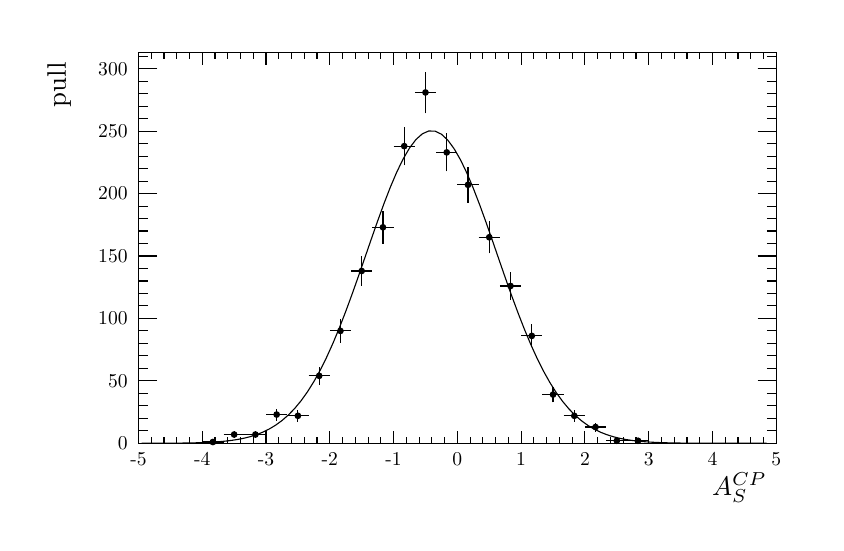
\begin{tikzpicture}
\pgfdeclareplotmark{cross} {
\pgfpathmoveto{\pgfpoint{-0.3\pgfplotmarksize}{\pgfplotmarksize}}
\pgfpathlineto{\pgfpoint{+0.3\pgfplotmarksize}{\pgfplotmarksize}}
\pgfpathlineto{\pgfpoint{+0.3\pgfplotmarksize}{0.3\pgfplotmarksize}}
\pgfpathlineto{\pgfpoint{+1\pgfplotmarksize}{0.3\pgfplotmarksize}}
\pgfpathlineto{\pgfpoint{+1\pgfplotmarksize}{-0.3\pgfplotmarksize}}
\pgfpathlineto{\pgfpoint{+0.3\pgfplotmarksize}{-0.3\pgfplotmarksize}}
\pgfpathlineto{\pgfpoint{+0.3\pgfplotmarksize}{-1.\pgfplotmarksize}}
\pgfpathlineto{\pgfpoint{-0.3\pgfplotmarksize}{-1.\pgfplotmarksize}}
\pgfpathlineto{\pgfpoint{-0.3\pgfplotmarksize}{-0.3\pgfplotmarksize}}
\pgfpathlineto{\pgfpoint{-1.\pgfplotmarksize}{-0.3\pgfplotmarksize}}
\pgfpathlineto{\pgfpoint{-1.\pgfplotmarksize}{0.3\pgfplotmarksize}}
\pgfpathlineto{\pgfpoint{-0.3\pgfplotmarksize}{0.3\pgfplotmarksize}}
\pgfpathclose
\pgfusepathqstroke
}
\pgfdeclareplotmark{cross*} {
\pgfpathmoveto{\pgfpoint{-0.3\pgfplotmarksize}{\pgfplotmarksize}}
\pgfpathlineto{\pgfpoint{+0.3\pgfplotmarksize}{\pgfplotmarksize}}
\pgfpathlineto{\pgfpoint{+0.3\pgfplotmarksize}{0.3\pgfplotmarksize}}
\pgfpathlineto{\pgfpoint{+1\pgfplotmarksize}{0.3\pgfplotmarksize}}
\pgfpathlineto{\pgfpoint{+1\pgfplotmarksize}{-0.3\pgfplotmarksize}}
\pgfpathlineto{\pgfpoint{+0.3\pgfplotmarksize}{-0.3\pgfplotmarksize}}
\pgfpathlineto{\pgfpoint{+0.3\pgfplotmarksize}{-1.\pgfplotmarksize}}
\pgfpathlineto{\pgfpoint{-0.3\pgfplotmarksize}{-1.\pgfplotmarksize}}
\pgfpathlineto{\pgfpoint{-0.3\pgfplotmarksize}{-0.3\pgfplotmarksize}}
\pgfpathlineto{\pgfpoint{-1.\pgfplotmarksize}{-0.3\pgfplotmarksize}}
\pgfpathlineto{\pgfpoint{-1.\pgfplotmarksize}{0.3\pgfplotmarksize}}
\pgfpathlineto{\pgfpoint{-0.3\pgfplotmarksize}{0.3\pgfplotmarksize}}
\pgfpathclose
\pgfusepathqfillstroke
}
\pgfdeclareplotmark{newstar} {
\pgfpathmoveto{\pgfqpoint{0pt}{\pgfplotmarksize}}
\pgfpathlineto{\pgfqpointpolar{44}{0.5\pgfplotmarksize}}
\pgfpathlineto{\pgfqpointpolar{18}{\pgfplotmarksize}}
\pgfpathlineto{\pgfqpointpolar{-20}{0.5\pgfplotmarksize}}
\pgfpathlineto{\pgfqpointpolar{-54}{\pgfplotmarksize}}
\pgfpathlineto{\pgfqpointpolar{-90}{0.5\pgfplotmarksize}}
\pgfpathlineto{\pgfqpointpolar{234}{\pgfplotmarksize}}
\pgfpathlineto{\pgfqpointpolar{198}{0.5\pgfplotmarksize}}
\pgfpathlineto{\pgfqpointpolar{162}{\pgfplotmarksize}}
\pgfpathlineto{\pgfqpointpolar{134}{0.5\pgfplotmarksize}}
\pgfpathclose
\pgfusepathqstroke
}
\pgfdeclareplotmark{newstar*} {
\pgfpathmoveto{\pgfqpoint{0pt}{\pgfplotmarksize}}
\pgfpathlineto{\pgfqpointpolar{44}{0.5\pgfplotmarksize}}
\pgfpathlineto{\pgfqpointpolar{18}{\pgfplotmarksize}}
\pgfpathlineto{\pgfqpointpolar{-20}{0.5\pgfplotmarksize}}
\pgfpathlineto{\pgfqpointpolar{-54}{\pgfplotmarksize}}
\pgfpathlineto{\pgfqpointpolar{-90}{0.5\pgfplotmarksize}}
\pgfpathlineto{\pgfqpointpolar{234}{\pgfplotmarksize}}
\pgfpathlineto{\pgfqpointpolar{198}{0.5\pgfplotmarksize}}
\pgfpathlineto{\pgfqpointpolar{162}{\pgfplotmarksize}}
\pgfpathlineto{\pgfqpointpolar{134}{0.5\pgfplotmarksize}}
\pgfpathclose
\pgfusepathqfillstroke
}
\definecolor{c}{rgb}{1,1,1};
\draw [color=c, fill=c] (0,0) rectangle (10,6.27517);
\draw [color=c, fill=c] (1.4,1.00403) rectangle (9.5,5.96141);
\definecolor{c}{rgb}{0,0,0};
\draw [c] (1.4,1.00403) -- (1.4,5.96141) -- (9.5,5.96141) -- (9.5,1.00403) -- (1.4,1.00403);
\draw [c] (2.345,1.00403) -- (2.345,1.01988);
\draw [c] (2.345,1.01988) -- (2.345,1.03574);
\draw [c] (2.21,1.01988) -- (2.345,1.01988);
\draw [c] (2.345,1.01988) -- (2.48,1.01988);
\foreach \P in {(2.345,1.01988)}{\draw[mark options={color=c,fill=c},mark size=2.402402pt,mark=*,mark size=1pt] plot coordinates {\P};}
\draw [c] (2.615,1.07307) -- (2.615,1.11502);
\draw [c] (2.615,1.11502) -- (2.615,1.15697);
\draw [c] (2.48,1.11502) -- (2.615,1.11502);
\draw [c] (2.615,1.11502) -- (2.75,1.11502);
\foreach \P in {(2.615,1.11502)}{\draw[mark options={color=c,fill=c},mark size=2.402402pt,mark=*,mark size=1pt] plot coordinates {\P};}
\draw [c] (2.885,1.07307) -- (2.885,1.11502);
\draw [c] (2.885,1.11502) -- (2.885,1.15697);
\draw [c] (2.75,1.11502) -- (2.885,1.11502);
\draw [c] (2.885,1.11502) -- (3.02,1.11502);
\foreach \P in {(2.885,1.11502)}{\draw[mark options={color=c,fill=c},mark size=2.402402pt,mark=*,mark size=1pt] plot coordinates {\P};}
\draw [c] (3.155,1.29267) -- (3.155,1.36871);
\draw [c] (3.155,1.36871) -- (3.155,1.44476);
\draw [c] (3.02,1.36871) -- (3.155,1.36871);
\draw [c] (3.155,1.36871) -- (3.29,1.36871);
\foreach \P in {(3.155,1.36871)}{\draw[mark options={color=c,fill=c},mark size=2.402402pt,mark=*,mark size=1pt] plot coordinates {\P};}
\draw [c] (3.425,1.27849) -- (3.425,1.35286);
\draw [c] (3.425,1.35286) -- (3.425,1.42723);
\draw [c] (3.29,1.35286) -- (3.425,1.35286);
\draw [c] (3.425,1.35286) -- (3.56,1.35286);
\foreach \P in {(3.425,1.35286)}{\draw[mark options={color=c,fill=c},mark size=2.402402pt,mark=*,mark size=1pt] plot coordinates {\P};}
\draw [c] (3.695,1.74373) -- (3.695,1.86025);
\draw [c] (3.695,1.86025) -- (3.695,1.97677);
\draw [c] (3.56,1.86025) -- (3.695,1.86025);
\draw [c] (3.695,1.86025) -- (3.83,1.86025);
\foreach \P in {(3.695,1.86025)}{\draw[mark options={color=c,fill=c},mark size=2.402402pt,mark=*,mark size=1pt] plot coordinates {\P};}
\draw [c] (3.965,2.28064) -- (3.965,2.43106);
\draw [c] (3.965,2.43106) -- (3.965,2.58149);
\draw [c] (3.83,2.43106) -- (3.965,2.43106);
\draw [c] (3.965,2.43106) -- (4.1,2.43106);
\foreach \P in {(3.965,2.43106)}{\draw[mark options={color=c,fill=c},mark size=2.402402pt,mark=*,mark size=1pt] plot coordinates {\P};}
\draw [c] (4.235,3.00588) -- (4.235,3.19215);
\draw [c] (4.235,3.19215) -- (4.235,3.37841);
\draw [c] (4.1,3.19215) -- (4.235,3.19215);
\draw [c] (4.235,3.19215) -- (4.37,3.19215);
\foreach \P in {(4.235,3.19215)}{\draw[mark options={color=c,fill=c},mark size=2.402402pt,mark=*,mark size=1pt] plot coordinates {\P};}
\draw [c] (4.505,3.53855) -- (4.505,3.74711);
\draw [c] (4.505,3.74711) -- (4.505,3.95566);
\draw [c] (4.37,3.74711) -- (4.505,3.74711);
\draw [c] (4.505,3.74711) -- (4.64,3.74711);
\foreach \P in {(4.505,3.74711)}{\draw[mark options={color=c,fill=c},mark size=2.402402pt,mark=*,mark size=1pt] plot coordinates {\P};}
\draw [c] (4.775,4.53313) -- (4.775,4.77774);
\draw [c] (4.775,4.77774) -- (4.775,5.02236);
\draw [c] (4.64,4.77774) -- (4.775,4.77774);
\draw [c] (4.775,4.77774) -- (4.91,4.77774);
\foreach \P in {(4.775,4.77774)}{\draw[mark options={color=c,fill=c},mark size=2.402402pt,mark=*,mark size=1pt] plot coordinates {\P};}
\draw [c] (5.045,5.19376) -- (5.045,5.45955);
\draw [c] (5.045,5.45955) -- (5.045,5.72534);
\draw [c] (4.91,5.45955) -- (5.045,5.45955);
\draw [c] (5.045,5.45955) -- (5.18,5.45955);
\foreach \P in {(5.045,5.45955)}{\draw[mark options={color=c,fill=c},mark size=2.402402pt,mark=*,mark size=1pt] plot coordinates {\P};}
\draw [c] (5.315,4.45643) -- (5.315,4.69846);
\draw [c] (5.315,4.69846) -- (5.315,4.94049);
\draw [c] (5.18,4.69846) -- (5.315,4.69846);
\draw [c] (5.315,4.69846) -- (5.45,4.69846);
\foreach \P in {(5.315,4.69846)}{\draw[mark options={color=c,fill=c},mark size=2.402402pt,mark=*,mark size=1pt] plot coordinates {\P};}
\draw [c] (5.585,4.05808) -- (5.585,4.28621);
\draw [c] (5.585,4.28621) -- (5.585,4.51434);
\draw [c] (5.45,4.28621) -- (5.585,4.28621);
\draw [c] (5.585,4.28621) -- (5.72,4.28621);
\foreach \P in {(5.585,4.28621)}{\draw[mark options={color=c,fill=c},mark size=2.402402pt,mark=*,mark size=1pt] plot coordinates {\P};}
\draw [c] (5.855,3.41659) -- (5.855,3.62026);
\draw [c] (5.855,3.62026) -- (5.855,3.82393);
\draw [c] (5.72,3.62026) -- (5.855,3.62026);
\draw [c] (5.855,3.62026) -- (5.99,3.62026);
\foreach \P in {(5.855,3.62026)}{\draw[mark options={color=c,fill=c},mark size=2.402402pt,mark=*,mark size=1pt] plot coordinates {\P};}
\draw [c] (6.125,2.82389) -- (6.125,3.00188);
\draw [c] (6.125,3.00188) -- (6.125,3.17986);
\draw [c] (5.99,3.00188) -- (6.125,3.00188);
\draw [c] (6.125,3.00188) -- (6.26,3.00188);
\foreach \P in {(6.125,3.00188)}{\draw[mark options={color=c,fill=c},mark size=2.402402pt,mark=*,mark size=1pt] plot coordinates {\P};}
\draw [c] (6.395,2.2206) -- (6.395,2.36764);
\draw [c] (6.395,2.36764) -- (6.395,2.51468);
\draw [c] (6.26,2.36764) -- (6.395,2.36764);
\draw [c] (6.395,2.36764) -- (6.53,2.36764);
\foreach \P in {(6.395,2.36764)}{\draw[mark options={color=c,fill=c},mark size=2.402402pt,mark=*,mark size=1pt] plot coordinates {\P};}
\draw [c] (6.665,1.52339) -- (6.665,1.62241);
\draw [c] (6.665,1.62241) -- (6.665,1.72143);
\draw [c] (6.53,1.62241) -- (6.665,1.62241);
\draw [c] (6.665,1.62241) -- (6.8,1.62241);
\foreach \P in {(6.665,1.62241)}{\draw[mark options={color=c,fill=c},mark size=2.402402pt,mark=*,mark size=1pt] plot coordinates {\P};}
\draw [c] (6.935,1.27849) -- (6.935,1.35286);
\draw [c] (6.935,1.35286) -- (6.935,1.42723);
\draw [c] (6.8,1.35286) -- (6.935,1.35286);
\draw [c] (6.935,1.35286) -- (7.07,1.35286);
\foreach \P in {(6.935,1.35286)}{\draw[mark options={color=c,fill=c},mark size=2.402402pt,mark=*,mark size=1pt] plot coordinates {\P};}
\draw [c] (7.205,1.15298) -- (7.205,1.21015);
\draw [c] (7.205,1.21015) -- (7.205,1.26732);
\draw [c] (7.07,1.21015) -- (7.205,1.21015);
\draw [c] (7.205,1.21015) -- (7.34,1.21015);
\foreach \P in {(7.205,1.21015)}{\draw[mark options={color=c,fill=c},mark size=2.402402pt,mark=*,mark size=1pt] plot coordinates {\P};}
\draw [c] (7.475,1.01332) -- (7.475,1.03574);
\draw [c] (7.475,1.03574) -- (7.475,1.05816);
\draw [c] (7.34,1.03574) -- (7.475,1.03574);
\draw [c] (7.475,1.03574) -- (7.61,1.03574);
\foreach \P in {(7.475,1.03574)}{\draw[mark options={color=c,fill=c},mark size=2.402402pt,mark=*,mark size=1pt] plot coordinates {\P};}
\draw [c] (7.745,1.01332) -- (7.745,1.03574);
\draw [c] (7.745,1.03574) -- (7.745,1.05816);
\draw [c] (7.61,1.03574) -- (7.745,1.03574);
\draw [c] (7.745,1.03574) -- (7.88,1.03574);
\foreach \P in {(7.745,1.03574)}{\draw[mark options={color=c,fill=c},mark size=2.402402pt,mark=*,mark size=1pt] plot coordinates {\P};}
\draw [c,line width=0.4] (1.4405,1.00403) -- (1.5215,1.00403) -- (1.6025,1.00403) -- (1.6835,1.00477) -- (1.7645,1.00513) -- (1.8455,1.00566) -- (1.9265,1.00641) -- (2.0075,1.00749) -- (2.0885,1.00899) -- (2.1695,1.01109) -- (2.2505,1.01397) --
 (2.3315,1.0179) -- (2.4125,1.02321) -- (2.4935,1.03028) -- (2.5745,1.03962) -- (2.6555,1.05183) -- (2.7365,1.06762) -- (2.8175,1.08783) -- (2.8985,1.1134) -- (2.9795,1.14543) -- (3.0605,1.1851) -- (3.1415,1.23371) -- (3.2225,1.2926) --
 (3.3035,1.36315) -- (3.3845,1.44671) -- (3.4655,1.54454) -- (3.5465,1.65774) -- (3.6275,1.78714) -- (3.7085,1.93327) -- (3.7895,2.09622) -- (3.8705,2.27556) -- (3.9515,2.47032) -- (4.0325,2.67888) -- (4.1135,2.89896) -- (4.1945,3.12764) --
 (4.2755,3.36136) -- (4.3565,3.59599) -- (4.4375,3.82695) -- (4.5185,4.04934) -- (4.5995,4.25811) -- (4.6805,4.44822) -- (4.7615,4.61488) -- (4.8425,4.75372) -- (4.9235,4.86097) -- (5.0045,4.93368) -- (5.0855,4.96981) -- (5.1665,4.96832) --
 (5.2475,4.92926) -- (5.3285,4.85374) -- (5.4095,4.74388);
\draw [c,line width=0.4] (5.4095,4.74388) -- (5.4905,4.60271) -- (5.5715,4.43404) -- (5.6525,4.24228) -- (5.7335,4.03225) -- (5.8145,3.809) -- (5.8955,3.57758) -- (5.9765,3.34286) -- (6.0575,3.1094) -- (6.1385,2.88127) -- (6.2195,2.662) --
 (6.3005,2.45445) -- (6.3815,2.26086) -- (6.4625,2.08278) -- (6.5435,1.92115) -- (6.6245,1.77635) -- (6.7055,1.64824) -- (6.7865,1.53629) -- (6.8675,1.43963) -- (6.9485,1.35714) -- (7.0295,1.28755) -- (7.1105,1.22952) -- (7.1915,1.18167) --
 (7.2725,1.14265) -- (7.3535,1.11117) -- (7.4345,1.08606) -- (7.5155,1.06623) -- (7.5965,1.05075) -- (7.6775,1.03879) -- (7.7585,1.02965) -- (7.8395,1.02273) -- (7.9205,1.01755) -- (8.0015,1.01371) -- (8.0825,1.0109) -- (8.1635,1.00886) --
 (8.2445,1.00739) -- (8.3255,1.00634) -- (8.4065,1.00561) -- (8.4875,1.0051) -- (8.5685,1.00474) -- (8.6495,1.00403) -- (8.7305,1.00403) -- (8.8115,1.00403) -- (8.8925,1.00403) -- (8.9735,1.00403) -- (9.0545,1.00403) -- (9.1355,1.00403) --
 (9.2165,1.00403) -- (9.2975,1.00403) -- (9.3785,1.00403);
\draw [c,line width=0.4] (9.3785,1.00403) -- (9.4595,1.00403);
\draw [c,line width=0.4] (1.4,1.00403) -- (9.5,1.00403);
\draw [anchor= east] (9.5,0.441772) node[scale=0.96888, rotate=0]{$A^{CP}_{\text{S}}$};
\draw [c,line width=0.4] (1.4,1.15651) -- (1.4,1.00403);
\draw [c,line width=0.4] (1.562,1.08027) -- (1.562,1.00403);
\draw [c,line width=0.4] (1.724,1.08027) -- (1.724,1.00403);
\draw [c,line width=0.4] (1.886,1.08027) -- (1.886,1.00403);
\draw [c,line width=0.4] (2.048,1.08027) -- (2.048,1.00403);
\draw [c,line width=0.4] (2.21,1.15651) -- (2.21,1.00403);
\draw [c,line width=0.4] (2.372,1.08027) -- (2.372,1.00403);
\draw [c,line width=0.4] (2.534,1.08027) -- (2.534,1.00403);
\draw [c,line width=0.4] (2.696,1.08027) -- (2.696,1.00403);
\draw [c,line width=0.4] (2.858,1.08027) -- (2.858,1.00403);
\draw [c,line width=0.4] (3.02,1.15651) -- (3.02,1.00403);
\draw [c,line width=0.4] (3.182,1.08027) -- (3.182,1.00403);
\draw [c,line width=0.4] (3.344,1.08027) -- (3.344,1.00403);
\draw [c,line width=0.4] (3.506,1.08027) -- (3.506,1.00403);
\draw [c,line width=0.4] (3.668,1.08027) -- (3.668,1.00403);
\draw [c,line width=0.4] (3.83,1.15651) -- (3.83,1.00403);
\draw [c,line width=0.4] (3.992,1.08027) -- (3.992,1.00403);
\draw [c,line width=0.4] (4.154,1.08027) -- (4.154,1.00403);
\draw [c,line width=0.4] (4.316,1.08027) -- (4.316,1.00403);
\draw [c,line width=0.4] (4.478,1.08027) -- (4.478,1.00403);
\draw [c,line width=0.4] (4.64,1.15651) -- (4.64,1.00403);
\draw [c,line width=0.4] (4.802,1.08027) -- (4.802,1.00403);
\draw [c,line width=0.4] (4.964,1.08027) -- (4.964,1.00403);
\draw [c,line width=0.4] (5.126,1.08027) -- (5.126,1.00403);
\draw [c,line width=0.4] (5.288,1.08027) -- (5.288,1.00403);
\draw [c,line width=0.4] (5.45,1.15651) -- (5.45,1.00403);
\draw [c,line width=0.4] (5.612,1.08027) -- (5.612,1.00403);
\draw [c,line width=0.4] (5.774,1.08027) -- (5.774,1.00403);
\draw [c,line width=0.4] (5.936,1.08027) -- (5.936,1.00403);
\draw [c,line width=0.4] (6.098,1.08027) -- (6.098,1.00403);
\draw [c,line width=0.4] (6.26,1.15651) -- (6.26,1.00403);
\draw [c,line width=0.4] (6.422,1.08027) -- (6.422,1.00403);
\draw [c,line width=0.4] (6.584,1.08027) -- (6.584,1.00403);
\draw [c,line width=0.4] (6.746,1.08027) -- (6.746,1.00403);
\draw [c,line width=0.4] (6.908,1.08027) -- (6.908,1.00403);
\draw [c,line width=0.4] (7.07,1.15651) -- (7.07,1.00403);
\draw [c,line width=0.4] (7.232,1.08027) -- (7.232,1.00403);
\draw [c,line width=0.4] (7.394,1.08027) -- (7.394,1.00403);
\draw [c,line width=0.4] (7.556,1.08027) -- (7.556,1.00403);
\draw [c,line width=0.4] (7.718,1.08027) -- (7.718,1.00403);
\draw [c,line width=0.4] (7.88,1.15651) -- (7.88,1.00403);
\draw [c,line width=0.4] (8.042,1.08027) -- (8.042,1.00403);
\draw [c,line width=0.4] (8.204,1.08027) -- (8.204,1.00403);
\draw [c,line width=0.4] (8.366,1.08027) -- (8.366,1.00403);
\draw [c,line width=0.4] (8.528,1.08027) -- (8.528,1.00403);
\draw [c,line width=0.4] (8.69,1.15651) -- (8.69,1.00403);
\draw [c,line width=0.4] (8.852,1.08027) -- (8.852,1.00403);
\draw [c,line width=0.4] (9.014,1.08027) -- (9.014,1.00403);
\draw [c,line width=0.4] (9.176,1.08027) -- (9.176,1.00403);
\draw [c,line width=0.4] (9.338,1.08027) -- (9.338,1.00403);
\draw [c,line width=0.4] (9.5,1.15651) -- (9.5,1.00403);
\draw [anchor=base] (1.4,0.721644) node[scale=0.708027, rotate=0]{-5};
\draw [anchor=base] (2.21,0.721644) node[scale=0.708027, rotate=0]{-4};
\draw [anchor=base] (3.02,0.721644) node[scale=0.708027, rotate=0]{-3};
\draw [anchor=base] (3.83,0.721644) node[scale=0.708027, rotate=0]{-2};
\draw [anchor=base] (4.64,0.721644) node[scale=0.708027, rotate=0]{-1};
\draw [anchor=base] (5.45,0.721644) node[scale=0.708027, rotate=0]{0};
\draw [anchor=base] (6.26,0.721644) node[scale=0.708027, rotate=0]{1};
\draw [anchor=base] (7.07,0.721644) node[scale=0.708027, rotate=0]{2};
\draw [anchor=base] (7.88,0.721644) node[scale=0.708027, rotate=0]{3};
\draw [anchor=base] (8.69,0.721644) node[scale=0.708027, rotate=0]{4};
\draw [anchor=base] (9.5,0.721644) node[scale=0.708027, rotate=0]{5};
\draw [c,line width=0.4] (1.4,5.96141) -- (9.5,5.96141);
\draw [c,line width=0.4] (1.4,5.80892) -- (1.4,5.96141);
\draw [c,line width=0.4] (1.562,5.88517) -- (1.562,5.96141);
\draw [c,line width=0.4] (1.724,5.88517) -- (1.724,5.96141);
\draw [c,line width=0.4] (1.886,5.88517) -- (1.886,5.96141);
\draw [c,line width=0.4] (2.048,5.88517) -- (2.048,5.96141);
\draw [c,line width=0.4] (2.21,5.80892) -- (2.21,5.96141);
\draw [c,line width=0.4] (2.372,5.88517) -- (2.372,5.96141);
\draw [c,line width=0.4] (2.534,5.88517) -- (2.534,5.96141);
\draw [c,line width=0.4] (2.696,5.88517) -- (2.696,5.96141);
\draw [c,line width=0.4] (2.858,5.88517) -- (2.858,5.96141);
\draw [c,line width=0.4] (3.02,5.80892) -- (3.02,5.96141);
\draw [c,line width=0.4] (3.182,5.88517) -- (3.182,5.96141);
\draw [c,line width=0.4] (3.344,5.88517) -- (3.344,5.96141);
\draw [c,line width=0.4] (3.506,5.88517) -- (3.506,5.96141);
\draw [c,line width=0.4] (3.668,5.88517) -- (3.668,5.96141);
\draw [c,line width=0.4] (3.83,5.80892) -- (3.83,5.96141);
\draw [c,line width=0.4] (3.992,5.88517) -- (3.992,5.96141);
\draw [c,line width=0.4] (4.154,5.88517) -- (4.154,5.96141);
\draw [c,line width=0.4] (4.316,5.88517) -- (4.316,5.96141);
\draw [c,line width=0.4] (4.478,5.88517) -- (4.478,5.96141);
\draw [c,line width=0.4] (4.64,5.80892) -- (4.64,5.96141);
\draw [c,line width=0.4] (4.802,5.88517) -- (4.802,5.96141);
\draw [c,line width=0.4] (4.964,5.88517) -- (4.964,5.96141);
\draw [c,line width=0.4] (5.126,5.88517) -- (5.126,5.96141);
\draw [c,line width=0.4] (5.288,5.88517) -- (5.288,5.96141);
\draw [c,line width=0.4] (5.45,5.80892) -- (5.45,5.96141);
\draw [c,line width=0.4] (5.612,5.88517) -- (5.612,5.96141);
\draw [c,line width=0.4] (5.774,5.88517) -- (5.774,5.96141);
\draw [c,line width=0.4] (5.936,5.88517) -- (5.936,5.96141);
\draw [c,line width=0.4] (6.098,5.88517) -- (6.098,5.96141);
\draw [c,line width=0.4] (6.26,5.80892) -- (6.26,5.96141);
\draw [c,line width=0.4] (6.422,5.88517) -- (6.422,5.96141);
\draw [c,line width=0.4] (6.584,5.88517) -- (6.584,5.96141);
\draw [c,line width=0.4] (6.746,5.88517) -- (6.746,5.96141);
\draw [c,line width=0.4] (6.908,5.88517) -- (6.908,5.96141);
\draw [c,line width=0.4] (7.07,5.80892) -- (7.07,5.96141);
\draw [c,line width=0.4] (7.232,5.88517) -- (7.232,5.96141);
\draw [c,line width=0.4] (7.394,5.88517) -- (7.394,5.96141);
\draw [c,line width=0.4] (7.556,5.88517) -- (7.556,5.96141);
\draw [c,line width=0.4] (7.718,5.88517) -- (7.718,5.96141);
\draw [c,line width=0.4] (7.88,5.80892) -- (7.88,5.96141);
\draw [c,line width=0.4] (8.042,5.88517) -- (8.042,5.96141);
\draw [c,line width=0.4] (8.204,5.88517) -- (8.204,5.96141);
\draw [c,line width=0.4] (8.366,5.88517) -- (8.366,5.96141);
\draw [c,line width=0.4] (8.528,5.88517) -- (8.528,5.96141);
\draw [c,line width=0.4] (8.69,5.80892) -- (8.69,5.96141);
\draw [c,line width=0.4] (8.852,5.88517) -- (8.852,5.96141);
\draw [c,line width=0.4] (9.014,5.88517) -- (9.014,5.96141);
\draw [c,line width=0.4] (9.176,5.88517) -- (9.176,5.96141);
\draw [c,line width=0.4] (9.338,5.88517) -- (9.338,5.96141);
\draw [c,line width=0.4] (9.5,5.80892) -- (9.5,5.96141);
\draw [c,line width=0.4] (1.4,1.00403) -- (1.4,5.96141);
\draw [anchor= east] (0.392,5.96141) node[scale=0.96888, rotate=90]{pull};
\draw [c,line width=0.4] (1.637,1.00403) -- (1.4,1.00403);
\draw [c,line width=0.4] (1.5185,1.16259) -- (1.4,1.16259);
\draw [c,line width=0.4] (1.5185,1.32115) -- (1.4,1.32115);
\draw [c,line width=0.4] (1.5185,1.47971) -- (1.4,1.47971);
\draw [c,line width=0.4] (1.5185,1.63826) -- (1.4,1.63826);
\draw [c,line width=0.4] (1.637,1.79682) -- (1.4,1.79682);
\draw [c,line width=0.4] (1.5185,1.95538) -- (1.4,1.95538);
\draw [c,line width=0.4] (1.5185,2.11394) -- (1.4,2.11394);
\draw [c,line width=0.4] (1.5185,2.2725) -- (1.4,2.2725);
\draw [c,line width=0.4] (1.5185,2.43106) -- (1.4,2.43106);
\draw [c,line width=0.4] (1.637,2.58962) -- (1.4,2.58962);
\draw [c,line width=0.4] (1.5185,2.74818) -- (1.4,2.74818);
\draw [c,line width=0.4] (1.5185,2.90674) -- (1.4,2.90674);
\draw [c,line width=0.4] (1.5185,3.0653) -- (1.4,3.0653);
\draw [c,line width=0.4] (1.5185,3.22386) -- (1.4,3.22386);
\draw [c,line width=0.4] (1.637,3.38242) -- (1.4,3.38242);
\draw [c,line width=0.4] (1.5185,3.54098) -- (1.4,3.54098);
\draw [c,line width=0.4] (1.5185,3.69954) -- (1.4,3.69954);
\draw [c,line width=0.4] (1.5185,3.8581) -- (1.4,3.8581);
\draw [c,line width=0.4] (1.5185,4.01666) -- (1.4,4.01666);
\draw [c,line width=0.4] (1.637,4.17522) -- (1.4,4.17522);
\draw [c,line width=0.4] (1.5185,4.33378) -- (1.4,4.33378);
\draw [c,line width=0.4] (1.5185,4.49234) -- (1.4,4.49234);
\draw [c,line width=0.4] (1.5185,4.6509) -- (1.4,4.6509);
\draw [c,line width=0.4] (1.5185,4.80946) -- (1.4,4.80946);
\draw [c,line width=0.4] (1.637,4.96802) -- (1.4,4.96802);
\draw [c,line width=0.4] (1.5185,5.12657) -- (1.4,5.12657);
\draw [c,line width=0.4] (1.5185,5.28513) -- (1.4,5.28513);
\draw [c,line width=0.4] (1.5185,5.44369) -- (1.4,5.44369);
\draw [c,line width=0.4] (1.5185,5.60225) -- (1.4,5.60225);
\draw [c,line width=0.4] (1.637,5.76081) -- (1.4,5.76081);
\draw [c,line width=0.4] (1.637,5.76081) -- (1.4,5.76081);
\draw [c,line width=0.4] (1.5185,5.91937) -- (1.4,5.91937);
\draw [anchor= east] (1.35,1.00403) node[scale=0.708027, rotate=0]{0};
\draw [anchor= east] (1.35,1.79682) node[scale=0.708027, rotate=0]{50};
\draw [anchor= east] (1.35,2.58962) node[scale=0.708027, rotate=0]{100};
\draw [anchor= east] (1.35,3.38242) node[scale=0.708027, rotate=0]{150};
\draw [anchor= east] (1.35,4.17522) node[scale=0.708027, rotate=0]{200};
\draw [anchor= east] (1.35,4.96802) node[scale=0.708027, rotate=0]{250};
\draw [anchor= east] (1.35,5.76081) node[scale=0.708027, rotate=0]{300};
\draw [c,line width=0.4] (9.5,1.00403) -- (9.5,5.96141);
\draw [c,line width=0.4] (9.263,1.00403) -- (9.5,1.00403);
\draw [c,line width=0.4] (9.3815,1.16259) -- (9.5,1.16259);
\draw [c,line width=0.4] (9.3815,1.32115) -- (9.5,1.32115);
\draw [c,line width=0.4] (9.3815,1.47971) -- (9.5,1.47971);
\draw [c,line width=0.4] (9.3815,1.63826) -- (9.5,1.63826);
\draw [c,line width=0.4] (9.263,1.79682) -- (9.5,1.79682);
\draw [c,line width=0.4] (9.3815,1.95538) -- (9.5,1.95538);
\draw [c,line width=0.4] (9.3815,2.11394) -- (9.5,2.11394);
\draw [c,line width=0.4] (9.3815,2.2725) -- (9.5,2.2725);
\draw [c,line width=0.4] (9.3815,2.43106) -- (9.5,2.43106);
\draw [c,line width=0.4] (9.263,2.58962) -- (9.5,2.58962);
\draw [c,line width=0.4] (9.3815,2.74818) -- (9.5,2.74818);
\draw [c,line width=0.4] (9.3815,2.90674) -- (9.5,2.90674);
\draw [c,line width=0.4] (9.3815,3.0653) -- (9.5,3.0653);
\draw [c,line width=0.4] (9.3815,3.22386) -- (9.5,3.22386);
\draw [c,line width=0.4] (9.263,3.38242) -- (9.5,3.38242);
\draw [c,line width=0.4] (9.3815,3.54098) -- (9.5,3.54098);
\draw [c,line width=0.4] (9.3815,3.69954) -- (9.5,3.69954);
\draw [c,line width=0.4] (9.3815,3.8581) -- (9.5,3.8581);
\draw [c,line width=0.4] (9.3815,4.01666) -- (9.5,4.01666);
\draw [c,line width=0.4] (9.263,4.17522) -- (9.5,4.17522);
\draw [c,line width=0.4] (9.3815,4.33378) -- (9.5,4.33378);
\draw [c,line width=0.4] (9.3815,4.49234) -- (9.5,4.49234);
\draw [c,line width=0.4] (9.3815,4.6509) -- (9.5,4.6509);
\draw [c,line width=0.4] (9.3815,4.80946) -- (9.5,4.80946);
\draw [c,line width=0.4] (9.263,4.96802) -- (9.5,4.96802);
\draw [c,line width=0.4] (9.3815,5.12657) -- (9.5,5.12657);
\draw [c,line width=0.4] (9.3815,5.28513) -- (9.5,5.28513);
\draw [c,line width=0.4] (9.3815,5.44369) -- (9.5,5.44369);
\draw [c,line width=0.4] (9.3815,5.60225) -- (9.5,5.60225);
\draw [c,line width=0.4] (9.263,5.76081) -- (9.5,5.76081);
\draw [c,line width=0.4] (9.263,5.76081) -- (9.5,5.76081);
\draw [c,line width=0.4] (9.3815,5.91937) -- (9.5,5.91937);
\end{tikzpicture}
}
    \caption{}
    \label{pull_ACPS}
  \end{subfigure}
\caption{Pull distributions of the parameters of the \Acp{i} interest. The distributions imply that the corresponding paramters are gaussian distributed.}
\label{pull_acp}
\end{figure}

In the curent toy experiments study the angular \pdf is used to generate datasets of $\Omega = (\cos\thetaK,\cos\thetamu,\phihel)$ 
distributions. The generated dataset is fitted again with the same \pdf and a new set of fitted parameters is obtained. Potential
biases on the parameters of intereset are estimated based on the {\it pull} variable of \equref{pull_def}.

\begin{equation}
P^i = \frac{p^{\rm gen} - p^i}{ \sigma^i },\;\;\left. 
  \begin{array}{ll}
    \sigma^i = \sigma^i_- \;\;{\rm if}\;\; p^{\rm gen} > p^i  \\
    \sigma^i = \sigma^i_+ \;\;{\rm if}\;\; p^{\rm gen} < p^i 
  \end{array} \right. ,
\label{pull_def}
\end{equation}

\noindent where, $p^{\rm gen}$ and $p^i$ are the generated and fitted (from each toy experiment) values of a given parameter of interest
respectivelly. The upper (lower) uncertainties $\sigma^i_+$($\sigma^i_-$) are used in case $p^i$ is on the left (right) side of the minimum.
Essentially the pull variale expresses the generated - fitted parameter value difference in units of one standard deviation. 

\begin{figure}[h]
  \centering
  \begin{subfigure}{0.5\textwidth}
    \tikzsetnextfilename{pull_f0}
    \scalebox{0.60}{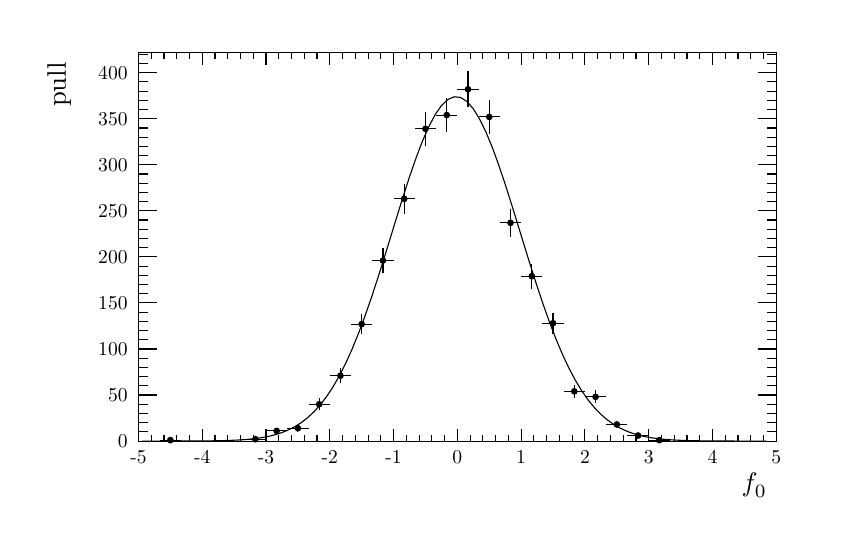
\begin{tikzpicture}
\pgfdeclareplotmark{cross} {
\pgfpathmoveto{\pgfpoint{-0.3\pgfplotmarksize}{\pgfplotmarksize}}
\pgfpathlineto{\pgfpoint{+0.3\pgfplotmarksize}{\pgfplotmarksize}}
\pgfpathlineto{\pgfpoint{+0.3\pgfplotmarksize}{0.3\pgfplotmarksize}}
\pgfpathlineto{\pgfpoint{+1\pgfplotmarksize}{0.3\pgfplotmarksize}}
\pgfpathlineto{\pgfpoint{+1\pgfplotmarksize}{-0.3\pgfplotmarksize}}
\pgfpathlineto{\pgfpoint{+0.3\pgfplotmarksize}{-0.3\pgfplotmarksize}}
\pgfpathlineto{\pgfpoint{+0.3\pgfplotmarksize}{-1.\pgfplotmarksize}}
\pgfpathlineto{\pgfpoint{-0.3\pgfplotmarksize}{-1.\pgfplotmarksize}}
\pgfpathlineto{\pgfpoint{-0.3\pgfplotmarksize}{-0.3\pgfplotmarksize}}
\pgfpathlineto{\pgfpoint{-1.\pgfplotmarksize}{-0.3\pgfplotmarksize}}
\pgfpathlineto{\pgfpoint{-1.\pgfplotmarksize}{0.3\pgfplotmarksize}}
\pgfpathlineto{\pgfpoint{-0.3\pgfplotmarksize}{0.3\pgfplotmarksize}}
\pgfpathclose
\pgfusepathqstroke
}
\pgfdeclareplotmark{cross*} {
\pgfpathmoveto{\pgfpoint{-0.3\pgfplotmarksize}{\pgfplotmarksize}}
\pgfpathlineto{\pgfpoint{+0.3\pgfplotmarksize}{\pgfplotmarksize}}
\pgfpathlineto{\pgfpoint{+0.3\pgfplotmarksize}{0.3\pgfplotmarksize}}
\pgfpathlineto{\pgfpoint{+1\pgfplotmarksize}{0.3\pgfplotmarksize}}
\pgfpathlineto{\pgfpoint{+1\pgfplotmarksize}{-0.3\pgfplotmarksize}}
\pgfpathlineto{\pgfpoint{+0.3\pgfplotmarksize}{-0.3\pgfplotmarksize}}
\pgfpathlineto{\pgfpoint{+0.3\pgfplotmarksize}{-1.\pgfplotmarksize}}
\pgfpathlineto{\pgfpoint{-0.3\pgfplotmarksize}{-1.\pgfplotmarksize}}
\pgfpathlineto{\pgfpoint{-0.3\pgfplotmarksize}{-0.3\pgfplotmarksize}}
\pgfpathlineto{\pgfpoint{-1.\pgfplotmarksize}{-0.3\pgfplotmarksize}}
\pgfpathlineto{\pgfpoint{-1.\pgfplotmarksize}{0.3\pgfplotmarksize}}
\pgfpathlineto{\pgfpoint{-0.3\pgfplotmarksize}{0.3\pgfplotmarksize}}
\pgfpathclose
\pgfusepathqfillstroke
}
\pgfdeclareplotmark{newstar} {
\pgfpathmoveto{\pgfqpoint{0pt}{\pgfplotmarksize}}
\pgfpathlineto{\pgfqpointpolar{44}{0.5\pgfplotmarksize}}
\pgfpathlineto{\pgfqpointpolar{18}{\pgfplotmarksize}}
\pgfpathlineto{\pgfqpointpolar{-20}{0.5\pgfplotmarksize}}
\pgfpathlineto{\pgfqpointpolar{-54}{\pgfplotmarksize}}
\pgfpathlineto{\pgfqpointpolar{-90}{0.5\pgfplotmarksize}}
\pgfpathlineto{\pgfqpointpolar{234}{\pgfplotmarksize}}
\pgfpathlineto{\pgfqpointpolar{198}{0.5\pgfplotmarksize}}
\pgfpathlineto{\pgfqpointpolar{162}{\pgfplotmarksize}}
\pgfpathlineto{\pgfqpointpolar{134}{0.5\pgfplotmarksize}}
\pgfpathclose
\pgfusepathqstroke
}
\pgfdeclareplotmark{newstar*} {
\pgfpathmoveto{\pgfqpoint{0pt}{\pgfplotmarksize}}
\pgfpathlineto{\pgfqpointpolar{44}{0.5\pgfplotmarksize}}
\pgfpathlineto{\pgfqpointpolar{18}{\pgfplotmarksize}}
\pgfpathlineto{\pgfqpointpolar{-20}{0.5\pgfplotmarksize}}
\pgfpathlineto{\pgfqpointpolar{-54}{\pgfplotmarksize}}
\pgfpathlineto{\pgfqpointpolar{-90}{0.5\pgfplotmarksize}}
\pgfpathlineto{\pgfqpointpolar{234}{\pgfplotmarksize}}
\pgfpathlineto{\pgfqpointpolar{198}{0.5\pgfplotmarksize}}
\pgfpathlineto{\pgfqpointpolar{162}{\pgfplotmarksize}}
\pgfpathlineto{\pgfqpointpolar{134}{0.5\pgfplotmarksize}}
\pgfpathclose
\pgfusepathqfillstroke
}
\definecolor{c}{rgb}{1,1,1};
\draw [color=c, fill=c] (0,0) rectangle (10,6.24161);
\draw [color=c, fill=c] (1.4,0.998658) rectangle (9.5,5.92953);
\definecolor{c}{rgb}{0,0,0};
\draw [c] (1.4,0.998658) -- (1.4,5.92953) -- (9.5,5.92953) -- (9.5,0.998658) -- (1.4,0.998658);
\draw [c] (1.805,0.998658) -- (1.805,1.01035);
\draw [c] (1.805,1.01035) -- (1.805,1.02205);
\draw [c] (1.67,1.01035) -- (1.805,1.01035);
\draw [c] (1.805,1.01035) -- (1.94,1.01035);
\foreach \P in {(1.805,1.01035)}{\draw[mark options={color=c,fill=c},mark size=2.402402pt,mark=*,mark size=1pt] plot coordinates {\P};}
\draw [c] (2.885,1.00551) -- (2.885,1.02205);
\draw [c] (2.885,1.02205) -- (2.885,1.03859);
\draw [c] (2.75,1.02205) -- (2.885,1.02205);
\draw [c] (2.885,1.02205) -- (3.02,1.02205);
\foreach \P in {(2.885,1.02205)}{\draw[mark options={color=c,fill=c},mark size=2.402402pt,mark=*,mark size=1pt] plot coordinates {\P};}
\draw [c] (3.155,1.08851) -- (3.155,1.1273);
\draw [c] (3.155,1.1273) -- (3.155,1.16609);
\draw [c] (3.02,1.1273) -- (3.155,1.1273);
\draw [c] (3.155,1.1273) -- (3.29,1.1273);
\foreach \P in {(3.155,1.1273)}{\draw[mark options={color=c,fill=c},mark size=2.402402pt,mark=*,mark size=1pt] plot coordinates {\P};}
\draw [c] (3.425,1.11863) -- (3.425,1.16239);
\draw [c] (3.425,1.16239) -- (3.425,1.20615);
\draw [c] (3.29,1.16239) -- (3.425,1.16239);
\draw [c] (3.425,1.16239) -- (3.56,1.16239);
\foreach \P in {(3.425,1.16239)}{\draw[mark options={color=c,fill=c},mark size=2.402402pt,mark=*,mark size=1pt] plot coordinates {\P};}
\draw [c] (3.695,1.39249) -- (3.695,1.46646);
\draw [c] (3.695,1.46646) -- (3.695,1.54042);
\draw [c] (3.56,1.46646) -- (3.695,1.46646);
\draw [c] (3.695,1.46646) -- (3.83,1.46646);
\foreach \P in {(3.695,1.46646)}{\draw[mark options={color=c,fill=c},mark size=2.402402pt,mark=*,mark size=1pt] plot coordinates {\P};}
\draw [c] (3.965,1.73046) -- (3.965,1.829);
\draw [c] (3.965,1.829) -- (3.965,1.92755);
\draw [c] (3.83,1.829) -- (3.965,1.829);
\draw [c] (3.965,1.829) -- (4.1,1.829);
\foreach \P in {(3.965,1.829)}{\draw[mark options={color=c,fill=c},mark size=2.402402pt,mark=*,mark size=1pt] plot coordinates {\P};}
\draw [c] (4.235,2.35213) -- (4.235,2.48392);
\draw [c] (4.235,2.48392) -- (4.235,2.61572);
\draw [c] (4.1,2.48392) -- (4.235,2.48392);
\draw [c] (4.235,2.48392) -- (4.37,2.48392);
\foreach \P in {(4.235,2.48392)}{\draw[mark options={color=c,fill=c},mark size=2.402402pt,mark=*,mark size=1pt] plot coordinates {\P};}
\draw [c] (4.505,3.12715) -- (4.505,3.29088);
\draw [c] (4.505,3.29088) -- (4.505,3.45461);
\draw [c] (4.37,3.29088) -- (4.505,3.29088);
\draw [c] (4.505,3.29088) -- (4.64,3.29088);
\foreach \P in {(4.505,3.29088)}{\draw[mark options={color=c,fill=c},mark size=2.402402pt,mark=*,mark size=1pt] plot coordinates {\P};}
\draw [c] (4.775,3.88478) -- (4.775,4.07444);
\draw [c] (4.775,4.07444) -- (4.775,4.26411);
\draw [c] (4.64,4.07444) -- (4.775,4.07444);
\draw [c] (4.775,4.07444) -- (4.91,4.07444);
\foreach \P in {(4.775,4.07444)}{\draw[mark options={color=c,fill=c},mark size=2.402402pt,mark=*,mark size=1pt] plot coordinates {\P};}
\draw [c] (5.045,4.74794) -- (5.045,4.96326);
\draw [c] (5.045,4.96326) -- (5.045,5.17859);
\draw [c] (4.91,4.96326) -- (5.045,4.96326);
\draw [c] (5.045,4.96326) -- (5.18,4.96326);
\foreach \P in {(5.045,4.96326)}{\draw[mark options={color=c,fill=c},mark size=2.402402pt,mark=*,mark size=1pt] plot coordinates {\P};}
\draw [c] (5.315,4.91865) -- (5.315,5.13869);
\draw [c] (5.315,5.13869) -- (5.315,5.35873);
\draw [c] (5.18,5.13869) -- (5.315,5.13869);
\draw [c] (5.315,5.13869) -- (5.45,5.13869);
\foreach \P in {(5.315,5.13869)}{\draw[mark options={color=c,fill=c},mark size=2.402402pt,mark=*,mark size=1pt] plot coordinates {\P};}
\draw [c] (5.585,5.23757) -- (5.585,5.46615);
\draw [c] (5.585,5.46615) -- (5.585,5.69473);
\draw [c] (5.45,5.46615) -- (5.585,5.46615);
\draw [c] (5.585,5.46615) -- (5.72,5.46615);
\foreach \P in {(5.585,5.46615)}{\draw[mark options={color=c,fill=c},mark size=2.402402pt,mark=*,mark size=1pt] plot coordinates {\P};}
\draw [c] (5.855,4.89588) -- (5.855,5.1153);
\draw [c] (5.855,5.1153) -- (5.855,5.33472);
\draw [c] (5.72,5.1153) -- (5.855,5.1153);
\draw [c] (5.855,5.1153) -- (5.99,5.1153);
\foreach \P in {(5.855,5.1153)}{\draw[mark options={color=c,fill=c},mark size=2.402402pt,mark=*,mark size=1pt] plot coordinates {\P};}
\draw [c] (6.125,3.59033) -- (6.125,3.77037);
\draw [c] (6.125,3.77037) -- (6.125,3.95042);
\draw [c] (5.99,3.77037) -- (6.125,3.77037);
\draw [c] (6.125,3.77037) -- (6.26,3.77037);
\foreach \P in {(6.125,3.77037)}{\draw[mark options={color=c,fill=c},mark size=2.402402pt,mark=*,mark size=1pt] plot coordinates {\P};}
\draw [c] (6.395,2.9356) -- (6.395,3.09206);
\draw [c] (6.395,3.09206) -- (6.395,3.24853);
\draw [c] (6.26,3.09206) -- (6.395,3.09206);
\draw [c] (6.395,3.09206) -- (6.53,3.09206);
\foreach \P in {(6.395,3.09206)}{\draw[mark options={color=c,fill=c},mark size=2.402402pt,mark=*,mark size=1pt] plot coordinates {\P};}
\draw [c] (6.665,2.3633) -- (6.665,2.49562);
\draw [c] (6.665,2.49562) -- (6.665,2.62793);
\draw [c] (6.53,2.49562) -- (6.665,2.49562);
\draw [c] (6.665,2.49562) -- (6.8,2.49562);
\foreach \P in {(6.665,2.49562)}{\draw[mark options={color=c,fill=c},mark size=2.402402pt,mark=*,mark size=1pt] plot coordinates {\P};}
\draw [c] (6.935,1.54425) -- (6.935,1.63019);
\draw [c] (6.935,1.63019) -- (6.935,1.71613);
\draw [c] (6.8,1.63019) -- (6.935,1.63019);
\draw [c] (6.935,1.63019) -- (7.07,1.63019);
\foreach \P in {(6.935,1.63019)}{\draw[mark options={color=c,fill=c},mark size=2.402402pt,mark=*,mark size=1pt] plot coordinates {\P};}
\draw [c] (7.205,1.47899) -- (7.205,1.56002);
\draw [c] (7.205,1.56002) -- (7.205,1.64104);
\draw [c] (7.07,1.56002) -- (7.205,1.56002);
\draw [c] (7.205,1.56002) -- (7.34,1.56002);
\foreach \P in {(7.205,1.56002)}{\draw[mark options={color=c,fill=c},mark size=2.402402pt,mark=*,mark size=1pt] plot coordinates {\P};}
\draw [c] (7.475,1.15955) -- (7.475,1.20917);
\draw [c] (7.475,1.20917) -- (7.475,1.25879);
\draw [c] (7.34,1.20917) -- (7.475,1.20917);
\draw [c] (7.475,1.20917) -- (7.61,1.20917);
\foreach \P in {(7.475,1.20917)}{\draw[mark options={color=c,fill=c},mark size=2.402402pt,mark=*,mark size=1pt] plot coordinates {\P};}
\draw [c] (7.745,1.04018) -- (7.745,1.06883);
\draw [c] (7.745,1.06883) -- (7.745,1.09747);
\draw [c] (7.61,1.06883) -- (7.745,1.06883);
\draw [c] (7.745,1.06883) -- (7.88,1.06883);
\foreach \P in {(7.745,1.06883)}{\draw[mark options={color=c,fill=c},mark size=2.402402pt,mark=*,mark size=1pt] plot coordinates {\P};}
\draw [c] (8.015,0.998658) -- (8.015,1.01035);
\draw [c] (8.015,1.01035) -- (8.015,1.02205);
\draw [c] (7.88,1.01035) -- (8.015,1.01035);
\draw [c] (8.015,1.01035) -- (8.15,1.01035);
\foreach \P in {(8.015,1.01035)}{\draw[mark options={color=c,fill=c},mark size=2.402402pt,mark=*,mark size=1pt] plot coordinates {\P};}
\draw [c,line width=0.4] (1.4405,0.998658) -- (1.5215,0.998658) -- (1.6025,0.998658) -- (1.6835,0.998658) -- (1.7645,0.998658) -- (1.8455,0.998658) -- (1.9265,0.998658) -- (2.0075,0.999264) -- (2.0885,0.999575) -- (2.1695,1.00003) -- (2.2505,1.0007)
 -- (2.3315,1.00166) -- (2.4125,1.00303) -- (2.4935,1.00496) -- (2.5745,1.00765) -- (2.6555,1.01135) -- (2.7365,1.01642) -- (2.8175,1.02326) -- (2.8985,1.03239) -- (2.9795,1.04446) -- (3.0605,1.06023) -- (3.1415,1.08061) -- (3.2225,1.10667) --
 (3.3035,1.1396) -- (3.3845,1.18076) -- (3.4655,1.23161) -- (3.5465,1.29371) -- (3.6275,1.36869) -- (3.7085,1.45812) -- (3.7895,1.56354) -- (3.8705,1.68629) -- (3.9515,1.82744) -- (4.0325,1.9877) -- (4.1135,2.16729) -- (4.1945,2.36585) --
 (4.2755,2.58234) -- (4.3565,2.81499) -- (4.4375,3.06125) -- (4.5185,3.31775) -- (4.5995,3.58039) -- (4.6805,3.84438) -- (4.7615,4.10439) -- (4.8425,4.35466) -- (4.9235,4.58928) -- (5.0045,4.80236) -- (5.0855,4.98828) -- (5.1665,5.14194) --
 (5.2475,5.25902) -- (5.3285,5.33614) -- (5.4095,5.37102);
\draw [c,line width=0.4] (5.4095,5.37102) -- (5.4905,5.36265) -- (5.5715,5.31127) -- (5.6525,5.21839) -- (5.7335,5.08673) -- (5.8145,4.92005) -- (5.8955,4.72301) -- (5.9765,4.50093) -- (6.0575,4.25955) -- (6.1385,4.00483) -- (6.2195,3.74262) --
 (6.3005,3.47854) -- (6.3815,3.21774) -- (6.4625,2.96475) -- (6.5435,2.72339) -- (6.6245,2.49672) -- (6.7055,2.28698) -- (6.7865,2.09567) -- (6.8675,1.92353) -- (6.9485,1.77071) -- (7.0295,1.63677) -- (7.1105,1.52085) -- (7.1915,1.42178) --
 (7.2725,1.33811) -- (7.3535,1.2683) -- (7.4345,1.21073) -- (7.5155,1.1638) -- (7.5965,1.12599) -- (7.6775,1.09586) -- (7.7585,1.07213) -- (7.8395,1.05365) -- (7.9205,1.0394) -- (8.0015,1.02855) -- (8.0825,1.02038) -- (8.1635,1.01428) --
 (8.2445,1.00978) -- (8.3255,1.0065) -- (8.4065,1.00413) -- (8.4875,1.00244) -- (8.5685,1.00125) -- (8.6495,1.00041) -- (8.7305,0.999836) -- (8.8115,0.99944) -- (8.8925,0.999173) -- (8.9735,0.998658) -- (9.0545,0.998658) -- (9.1355,0.998658) --
 (9.2165,0.998658) -- (9.2975,0.998658) -- (9.3785,0.998658);
\draw [c,line width=0.4] (9.3785,0.998658) -- (9.4595,0.998658);
\draw [c,line width=0.4] (1.4,0.998658) -- (9.5,0.998658);
\draw [anchor= east] (9.5,0.439409) node[scale=0.96888, rotate=0]{$f_{0}^{\text{}}$};
\draw [c,line width=0.4] (1.4,1.15033) -- (1.4,0.998658);
\draw [c,line width=0.4] (1.562,1.07449) -- (1.562,0.998658);
\draw [c,line width=0.4] (1.724,1.07449) -- (1.724,0.998658);
\draw [c,line width=0.4] (1.886,1.07449) -- (1.886,0.998658);
\draw [c,line width=0.4] (2.048,1.07449) -- (2.048,0.998658);
\draw [c,line width=0.4] (2.21,1.15033) -- (2.21,0.998658);
\draw [c,line width=0.4] (2.372,1.07449) -- (2.372,0.998658);
\draw [c,line width=0.4] (2.534,1.07449) -- (2.534,0.998658);
\draw [c,line width=0.4] (2.696,1.07449) -- (2.696,0.998658);
\draw [c,line width=0.4] (2.858,1.07449) -- (2.858,0.998658);
\draw [c,line width=0.4] (3.02,1.15033) -- (3.02,0.998658);
\draw [c,line width=0.4] (3.182,1.07449) -- (3.182,0.998658);
\draw [c,line width=0.4] (3.344,1.07449) -- (3.344,0.998658);
\draw [c,line width=0.4] (3.506,1.07449) -- (3.506,0.998658);
\draw [c,line width=0.4] (3.668,1.07449) -- (3.668,0.998658);
\draw [c,line width=0.4] (3.83,1.15033) -- (3.83,0.998658);
\draw [c,line width=0.4] (3.992,1.07449) -- (3.992,0.998658);
\draw [c,line width=0.4] (4.154,1.07449) -- (4.154,0.998658);
\draw [c,line width=0.4] (4.316,1.07449) -- (4.316,0.998658);
\draw [c,line width=0.4] (4.478,1.07449) -- (4.478,0.998658);
\draw [c,line width=0.4] (4.64,1.15033) -- (4.64,0.998658);
\draw [c,line width=0.4] (4.802,1.07449) -- (4.802,0.998658);
\draw [c,line width=0.4] (4.964,1.07449) -- (4.964,0.998658);
\draw [c,line width=0.4] (5.126,1.07449) -- (5.126,0.998658);
\draw [c,line width=0.4] (5.288,1.07449) -- (5.288,0.998658);
\draw [c,line width=0.4] (5.45,1.15033) -- (5.45,0.998658);
\draw [c,line width=0.4] (5.612,1.07449) -- (5.612,0.998658);
\draw [c,line width=0.4] (5.774,1.07449) -- (5.774,0.998658);
\draw [c,line width=0.4] (5.936,1.07449) -- (5.936,0.998658);
\draw [c,line width=0.4] (6.098,1.07449) -- (6.098,0.998658);
\draw [c,line width=0.4] (6.26,1.15033) -- (6.26,0.998658);
\draw [c,line width=0.4] (6.422,1.07449) -- (6.422,0.998658);
\draw [c,line width=0.4] (6.584,1.07449) -- (6.584,0.998658);
\draw [c,line width=0.4] (6.746,1.07449) -- (6.746,0.998658);
\draw [c,line width=0.4] (6.908,1.07449) -- (6.908,0.998658);
\draw [c,line width=0.4] (7.07,1.15033) -- (7.07,0.998658);
\draw [c,line width=0.4] (7.232,1.07449) -- (7.232,0.998658);
\draw [c,line width=0.4] (7.394,1.07449) -- (7.394,0.998658);
\draw [c,line width=0.4] (7.556,1.07449) -- (7.556,0.998658);
\draw [c,line width=0.4] (7.718,1.07449) -- (7.718,0.998658);
\draw [c,line width=0.4] (7.88,1.15033) -- (7.88,0.998658);
\draw [c,line width=0.4] (8.042,1.07449) -- (8.042,0.998658);
\draw [c,line width=0.4] (8.204,1.07449) -- (8.204,0.998658);
\draw [c,line width=0.4] (8.366,1.07449) -- (8.366,0.998658);
\draw [c,line width=0.4] (8.528,1.07449) -- (8.528,0.998658);
\draw [c,line width=0.4] (8.69,1.15033) -- (8.69,0.998658);
\draw [c,line width=0.4] (8.852,1.07449) -- (8.852,0.998658);
\draw [c,line width=0.4] (9.014,1.07449) -- (9.014,0.998658);
\draw [c,line width=0.4] (9.176,1.07449) -- (9.176,0.998658);
\draw [c,line width=0.4] (9.338,1.07449) -- (9.338,0.998658);
\draw [c,line width=0.4] (9.5,1.15033) -- (9.5,0.998658);
\draw [anchor=base] (1.4,0.717785) node[scale=0.708027, rotate=0]{-5};
\draw [anchor=base] (2.21,0.717785) node[scale=0.708027, rotate=0]{-4};
\draw [anchor=base] (3.02,0.717785) node[scale=0.708027, rotate=0]{-3};
\draw [anchor=base] (3.83,0.717785) node[scale=0.708027, rotate=0]{-2};
\draw [anchor=base] (4.64,0.717785) node[scale=0.708027, rotate=0]{-1};
\draw [anchor=base] (5.45,0.717785) node[scale=0.708027, rotate=0]{0};
\draw [anchor=base] (6.26,0.717785) node[scale=0.708027, rotate=0]{1};
\draw [anchor=base] (7.07,0.717785) node[scale=0.708027, rotate=0]{2};
\draw [anchor=base] (7.88,0.717785) node[scale=0.708027, rotate=0]{3};
\draw [anchor=base] (8.69,0.717785) node[scale=0.708027, rotate=0]{4};
\draw [anchor=base] (9.5,0.717785) node[scale=0.708027, rotate=0]{5};
\draw [c,line width=0.4] (1.4,5.92953) -- (9.5,5.92953);
\draw [c,line width=0.4] (1.4,5.77786) -- (1.4,5.92953);
\draw [c,line width=0.4] (1.562,5.85369) -- (1.562,5.92953);
\draw [c,line width=0.4] (1.724,5.85369) -- (1.724,5.92953);
\draw [c,line width=0.4] (1.886,5.85369) -- (1.886,5.92953);
\draw [c,line width=0.4] (2.048,5.85369) -- (2.048,5.92953);
\draw [c,line width=0.4] (2.21,5.77786) -- (2.21,5.92953);
\draw [c,line width=0.4] (2.372,5.85369) -- (2.372,5.92953);
\draw [c,line width=0.4] (2.534,5.85369) -- (2.534,5.92953);
\draw [c,line width=0.4] (2.696,5.85369) -- (2.696,5.92953);
\draw [c,line width=0.4] (2.858,5.85369) -- (2.858,5.92953);
\draw [c,line width=0.4] (3.02,5.77786) -- (3.02,5.92953);
\draw [c,line width=0.4] (3.182,5.85369) -- (3.182,5.92953);
\draw [c,line width=0.4] (3.344,5.85369) -- (3.344,5.92953);
\draw [c,line width=0.4] (3.506,5.85369) -- (3.506,5.92953);
\draw [c,line width=0.4] (3.668,5.85369) -- (3.668,5.92953);
\draw [c,line width=0.4] (3.83,5.77786) -- (3.83,5.92953);
\draw [c,line width=0.4] (3.992,5.85369) -- (3.992,5.92953);
\draw [c,line width=0.4] (4.154,5.85369) -- (4.154,5.92953);
\draw [c,line width=0.4] (4.316,5.85369) -- (4.316,5.92953);
\draw [c,line width=0.4] (4.478,5.85369) -- (4.478,5.92953);
\draw [c,line width=0.4] (4.64,5.77786) -- (4.64,5.92953);
\draw [c,line width=0.4] (4.802,5.85369) -- (4.802,5.92953);
\draw [c,line width=0.4] (4.964,5.85369) -- (4.964,5.92953);
\draw [c,line width=0.4] (5.126,5.85369) -- (5.126,5.92953);
\draw [c,line width=0.4] (5.288,5.85369) -- (5.288,5.92953);
\draw [c,line width=0.4] (5.45,5.77786) -- (5.45,5.92953);
\draw [c,line width=0.4] (5.612,5.85369) -- (5.612,5.92953);
\draw [c,line width=0.4] (5.774,5.85369) -- (5.774,5.92953);
\draw [c,line width=0.4] (5.936,5.85369) -- (5.936,5.92953);
\draw [c,line width=0.4] (6.098,5.85369) -- (6.098,5.92953);
\draw [c,line width=0.4] (6.26,5.77786) -- (6.26,5.92953);
\draw [c,line width=0.4] (6.422,5.85369) -- (6.422,5.92953);
\draw [c,line width=0.4] (6.584,5.85369) -- (6.584,5.92953);
\draw [c,line width=0.4] (6.746,5.85369) -- (6.746,5.92953);
\draw [c,line width=0.4] (6.908,5.85369) -- (6.908,5.92953);
\draw [c,line width=0.4] (7.07,5.77786) -- (7.07,5.92953);
\draw [c,line width=0.4] (7.232,5.85369) -- (7.232,5.92953);
\draw [c,line width=0.4] (7.394,5.85369) -- (7.394,5.92953);
\draw [c,line width=0.4] (7.556,5.85369) -- (7.556,5.92953);
\draw [c,line width=0.4] (7.718,5.85369) -- (7.718,5.92953);
\draw [c,line width=0.4] (7.88,5.77786) -- (7.88,5.92953);
\draw [c,line width=0.4] (8.042,5.85369) -- (8.042,5.92953);
\draw [c,line width=0.4] (8.204,5.85369) -- (8.204,5.92953);
\draw [c,line width=0.4] (8.366,5.85369) -- (8.366,5.92953);
\draw [c,line width=0.4] (8.528,5.85369) -- (8.528,5.92953);
\draw [c,line width=0.4] (8.69,5.77786) -- (8.69,5.92953);
\draw [c,line width=0.4] (8.852,5.85369) -- (8.852,5.92953);
\draw [c,line width=0.4] (9.014,5.85369) -- (9.014,5.92953);
\draw [c,line width=0.4] (9.176,5.85369) -- (9.176,5.92953);
\draw [c,line width=0.4] (9.338,5.85369) -- (9.338,5.92953);
\draw [c,line width=0.4] (9.5,5.77786) -- (9.5,5.92953);
\draw [c,line width=0.4] (1.4,0.998658) -- (1.4,5.92953);
\draw [anchor= east] (0.392,5.92953) node[scale=0.96888, rotate=90]{pull};
\draw [c,line width=0.4] (1.637,0.998658) -- (1.4,0.998658);
\draw [c,line width=0.4] (1.5185,1.11561) -- (1.4,1.11561);
\draw [c,line width=0.4] (1.5185,1.23256) -- (1.4,1.23256);
\draw [c,line width=0.4] (1.5185,1.34951) -- (1.4,1.34951);
\draw [c,line width=0.4] (1.5185,1.46646) -- (1.4,1.46646);
\draw [c,line width=0.4] (1.637,1.58341) -- (1.4,1.58341);
\draw [c,line width=0.4] (1.5185,1.70036) -- (1.4,1.70036);
\draw [c,line width=0.4] (1.5185,1.81731) -- (1.4,1.81731);
\draw [c,line width=0.4] (1.5185,1.93426) -- (1.4,1.93426);
\draw [c,line width=0.4] (1.5185,2.05121) -- (1.4,2.05121);
\draw [c,line width=0.4] (1.637,2.16816) -- (1.4,2.16816);
\draw [c,line width=0.4] (1.5185,2.28511) -- (1.4,2.28511);
\draw [c,line width=0.4] (1.5185,2.40206) -- (1.4,2.40206);
\draw [c,line width=0.4] (1.5185,2.51901) -- (1.4,2.51901);
\draw [c,line width=0.4] (1.5185,2.63596) -- (1.4,2.63596);
\draw [c,line width=0.4] (1.637,2.75291) -- (1.4,2.75291);
\draw [c,line width=0.4] (1.5185,2.86986) -- (1.4,2.86986);
\draw [c,line width=0.4] (1.5185,2.98681) -- (1.4,2.98681);
\draw [c,line width=0.4] (1.5185,3.10376) -- (1.4,3.10376);
\draw [c,line width=0.4] (1.5185,3.22071) -- (1.4,3.22071);
\draw [c,line width=0.4] (1.637,3.33766) -- (1.4,3.33766);
\draw [c,line width=0.4] (1.5185,3.45461) -- (1.4,3.45461);
\draw [c,line width=0.4] (1.5185,3.57156) -- (1.4,3.57156);
\draw [c,line width=0.4] (1.5185,3.68851) -- (1.4,3.68851);
\draw [c,line width=0.4] (1.5185,3.80546) -- (1.4,3.80546);
\draw [c,line width=0.4] (1.637,3.92241) -- (1.4,3.92241);
\draw [c,line width=0.4] (1.5185,4.03936) -- (1.4,4.03936);
\draw [c,line width=0.4] (1.5185,4.15631) -- (1.4,4.15631);
\draw [c,line width=0.4] (1.5185,4.27326) -- (1.4,4.27326);
\draw [c,line width=0.4] (1.5185,4.39021) -- (1.4,4.39021);
\draw [c,line width=0.4] (1.637,4.50716) -- (1.4,4.50716);
\draw [c,line width=0.4] (1.5185,4.62411) -- (1.4,4.62411);
\draw [c,line width=0.4] (1.5185,4.74106) -- (1.4,4.74106);
\draw [c,line width=0.4] (1.5185,4.85801) -- (1.4,4.85801);
\draw [c,line width=0.4] (1.5185,4.97496) -- (1.4,4.97496);
\draw [c,line width=0.4] (1.637,5.09191) -- (1.4,5.09191);
\draw [c,line width=0.4] (1.5185,5.20886) -- (1.4,5.20886);
\draw [c,line width=0.4] (1.5185,5.32581) -- (1.4,5.32581);
\draw [c,line width=0.4] (1.5185,5.44276) -- (1.4,5.44276);
\draw [c,line width=0.4] (1.5185,5.55971) -- (1.4,5.55971);
\draw [c,line width=0.4] (1.637,5.67666) -- (1.4,5.67666);
\draw [c,line width=0.4] (1.637,5.67666) -- (1.4,5.67666);
\draw [c,line width=0.4] (1.5185,5.79361) -- (1.4,5.79361);
\draw [c,line width=0.4] (1.5185,5.91056) -- (1.4,5.91056);
\draw [anchor= east] (1.35,0.998658) node[scale=0.708027, rotate=0]{0};
\draw [anchor= east] (1.35,1.58341) node[scale=0.708027, rotate=0]{50};
\draw [anchor= east] (1.35,2.16816) node[scale=0.708027, rotate=0]{100};
\draw [anchor= east] (1.35,2.75291) node[scale=0.708027, rotate=0]{150};
\draw [anchor= east] (1.35,3.33766) node[scale=0.708027, rotate=0]{200};
\draw [anchor= east] (1.35,3.92241) node[scale=0.708027, rotate=0]{250};
\draw [anchor= east] (1.35,4.50716) node[scale=0.708027, rotate=0]{300};
\draw [anchor= east] (1.35,5.09191) node[scale=0.708027, rotate=0]{350};
\draw [anchor= east] (1.35,5.67666) node[scale=0.708027, rotate=0]{400};
\draw [c,line width=0.4] (9.5,0.998658) -- (9.5,5.92953);
\draw [c,line width=0.4] (9.263,0.998658) -- (9.5,0.998658);
\draw [c,line width=0.4] (9.3815,1.11561) -- (9.5,1.11561);
\draw [c,line width=0.4] (9.3815,1.23256) -- (9.5,1.23256);
\draw [c,line width=0.4] (9.3815,1.34951) -- (9.5,1.34951);
\draw [c,line width=0.4] (9.3815,1.46646) -- (9.5,1.46646);
\draw [c,line width=0.4] (9.263,1.58341) -- (9.5,1.58341);
\draw [c,line width=0.4] (9.3815,1.70036) -- (9.5,1.70036);
\draw [c,line width=0.4] (9.3815,1.81731) -- (9.5,1.81731);
\draw [c,line width=0.4] (9.3815,1.93426) -- (9.5,1.93426);
\draw [c,line width=0.4] (9.3815,2.05121) -- (9.5,2.05121);
\draw [c,line width=0.4] (9.263,2.16816) -- (9.5,2.16816);
\draw [c,line width=0.4] (9.3815,2.28511) -- (9.5,2.28511);
\draw [c,line width=0.4] (9.3815,2.40206) -- (9.5,2.40206);
\draw [c,line width=0.4] (9.3815,2.51901) -- (9.5,2.51901);
\draw [c,line width=0.4] (9.3815,2.63596) -- (9.5,2.63596);
\draw [c,line width=0.4] (9.263,2.75291) -- (9.5,2.75291);
\draw [c,line width=0.4] (9.3815,2.86986) -- (9.5,2.86986);
\draw [c,line width=0.4] (9.3815,2.98681) -- (9.5,2.98681);
\draw [c,line width=0.4] (9.3815,3.10376) -- (9.5,3.10376);
\draw [c,line width=0.4] (9.3815,3.22071) -- (9.5,3.22071);
\draw [c,line width=0.4] (9.263,3.33766) -- (9.5,3.33766);
\draw [c,line width=0.4] (9.3815,3.45461) -- (9.5,3.45461);
\draw [c,line width=0.4] (9.3815,3.57156) -- (9.5,3.57156);
\draw [c,line width=0.4] (9.3815,3.68851) -- (9.5,3.68851);
\draw [c,line width=0.4] (9.3815,3.80546) -- (9.5,3.80546);
\draw [c,line width=0.4] (9.263,3.92241) -- (9.5,3.92241);
\draw [c,line width=0.4] (9.3815,4.03936) -- (9.5,4.03936);
\draw [c,line width=0.4] (9.3815,4.15631) -- (9.5,4.15631);
\draw [c,line width=0.4] (9.3815,4.27326) -- (9.5,4.27326);
\draw [c,line width=0.4] (9.3815,4.39021) -- (9.5,4.39021);
\draw [c,line width=0.4] (9.263,4.50716) -- (9.5,4.50716);
\draw [c,line width=0.4] (9.3815,4.62411) -- (9.5,4.62411);
\draw [c,line width=0.4] (9.3815,4.74106) -- (9.5,4.74106);
\draw [c,line width=0.4] (9.3815,4.85801) -- (9.5,4.85801);
\draw [c,line width=0.4] (9.3815,4.97496) -- (9.5,4.97496);
\draw [c,line width=0.4] (9.263,5.09191) -- (9.5,5.09191);
\draw [c,line width=0.4] (9.3815,5.20886) -- (9.5,5.20886);
\draw [c,line width=0.4] (9.3815,5.32581) -- (9.5,5.32581);
\draw [c,line width=0.4] (9.3815,5.44276) -- (9.5,5.44276);
\draw [c,line width=0.4] (9.3815,5.55971) -- (9.5,5.55971);
\draw [c,line width=0.4] (9.263,5.67666) -- (9.5,5.67666);
\draw [c,line width=0.4] (9.263,5.67666) -- (9.5,5.67666);
\draw [c,line width=0.4] (9.3815,5.79361) -- (9.5,5.79361);
\draw [c,line width=0.4] (9.3815,5.91056) -- (9.5,5.91056);
\end{tikzpicture}
}
    \caption{}
    \label{pull_f0}
  \end{subfigure}%
  \hfill%
  \begin{subfigure}{0.5\textwidth}
    \tikzsetnextfilename{pull_fpar}
    \scalebox{0.60}{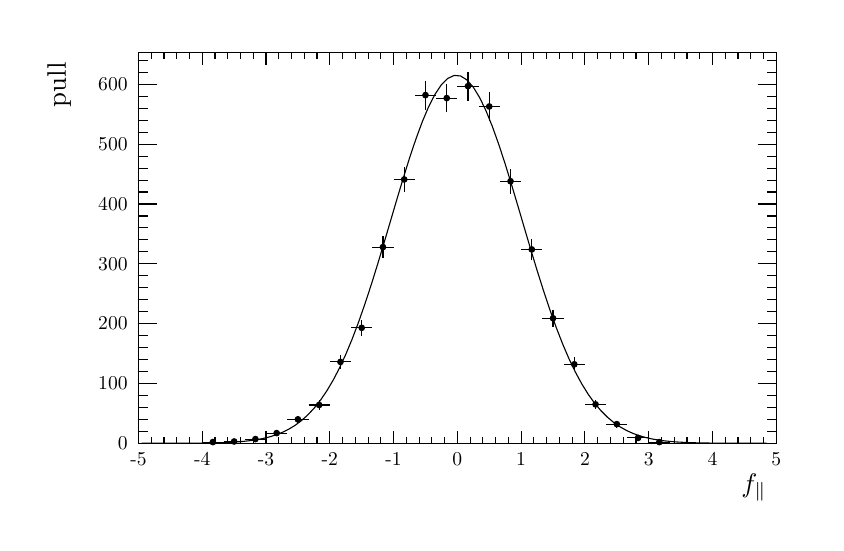
\begin{tikzpicture}
\pgfdeclareplotmark{cross} {
\pgfpathmoveto{\pgfpoint{-0.3\pgfplotmarksize}{\pgfplotmarksize}}
\pgfpathlineto{\pgfpoint{+0.3\pgfplotmarksize}{\pgfplotmarksize}}
\pgfpathlineto{\pgfpoint{+0.3\pgfplotmarksize}{0.3\pgfplotmarksize}}
\pgfpathlineto{\pgfpoint{+1\pgfplotmarksize}{0.3\pgfplotmarksize}}
\pgfpathlineto{\pgfpoint{+1\pgfplotmarksize}{-0.3\pgfplotmarksize}}
\pgfpathlineto{\pgfpoint{+0.3\pgfplotmarksize}{-0.3\pgfplotmarksize}}
\pgfpathlineto{\pgfpoint{+0.3\pgfplotmarksize}{-1.\pgfplotmarksize}}
\pgfpathlineto{\pgfpoint{-0.3\pgfplotmarksize}{-1.\pgfplotmarksize}}
\pgfpathlineto{\pgfpoint{-0.3\pgfplotmarksize}{-0.3\pgfplotmarksize}}
\pgfpathlineto{\pgfpoint{-1.\pgfplotmarksize}{-0.3\pgfplotmarksize}}
\pgfpathlineto{\pgfpoint{-1.\pgfplotmarksize}{0.3\pgfplotmarksize}}
\pgfpathlineto{\pgfpoint{-0.3\pgfplotmarksize}{0.3\pgfplotmarksize}}
\pgfpathclose
\pgfusepathqstroke
}
\pgfdeclareplotmark{cross*} {
\pgfpathmoveto{\pgfpoint{-0.3\pgfplotmarksize}{\pgfplotmarksize}}
\pgfpathlineto{\pgfpoint{+0.3\pgfplotmarksize}{\pgfplotmarksize}}
\pgfpathlineto{\pgfpoint{+0.3\pgfplotmarksize}{0.3\pgfplotmarksize}}
\pgfpathlineto{\pgfpoint{+1\pgfplotmarksize}{0.3\pgfplotmarksize}}
\pgfpathlineto{\pgfpoint{+1\pgfplotmarksize}{-0.3\pgfplotmarksize}}
\pgfpathlineto{\pgfpoint{+0.3\pgfplotmarksize}{-0.3\pgfplotmarksize}}
\pgfpathlineto{\pgfpoint{+0.3\pgfplotmarksize}{-1.\pgfplotmarksize}}
\pgfpathlineto{\pgfpoint{-0.3\pgfplotmarksize}{-1.\pgfplotmarksize}}
\pgfpathlineto{\pgfpoint{-0.3\pgfplotmarksize}{-0.3\pgfplotmarksize}}
\pgfpathlineto{\pgfpoint{-1.\pgfplotmarksize}{-0.3\pgfplotmarksize}}
\pgfpathlineto{\pgfpoint{-1.\pgfplotmarksize}{0.3\pgfplotmarksize}}
\pgfpathlineto{\pgfpoint{-0.3\pgfplotmarksize}{0.3\pgfplotmarksize}}
\pgfpathclose
\pgfusepathqfillstroke
}
\pgfdeclareplotmark{newstar} {
\pgfpathmoveto{\pgfqpoint{0pt}{\pgfplotmarksize}}
\pgfpathlineto{\pgfqpointpolar{44}{0.5\pgfplotmarksize}}
\pgfpathlineto{\pgfqpointpolar{18}{\pgfplotmarksize}}
\pgfpathlineto{\pgfqpointpolar{-20}{0.5\pgfplotmarksize}}
\pgfpathlineto{\pgfqpointpolar{-54}{\pgfplotmarksize}}
\pgfpathlineto{\pgfqpointpolar{-90}{0.5\pgfplotmarksize}}
\pgfpathlineto{\pgfqpointpolar{234}{\pgfplotmarksize}}
\pgfpathlineto{\pgfqpointpolar{198}{0.5\pgfplotmarksize}}
\pgfpathlineto{\pgfqpointpolar{162}{\pgfplotmarksize}}
\pgfpathlineto{\pgfqpointpolar{134}{0.5\pgfplotmarksize}}
\pgfpathclose
\pgfusepathqstroke
}
\pgfdeclareplotmark{newstar*} {
\pgfpathmoveto{\pgfqpoint{0pt}{\pgfplotmarksize}}
\pgfpathlineto{\pgfqpointpolar{44}{0.5\pgfplotmarksize}}
\pgfpathlineto{\pgfqpointpolar{18}{\pgfplotmarksize}}
\pgfpathlineto{\pgfqpointpolar{-20}{0.5\pgfplotmarksize}}
\pgfpathlineto{\pgfqpointpolar{-54}{\pgfplotmarksize}}
\pgfpathlineto{\pgfqpointpolar{-90}{0.5\pgfplotmarksize}}
\pgfpathlineto{\pgfqpointpolar{234}{\pgfplotmarksize}}
\pgfpathlineto{\pgfqpointpolar{198}{0.5\pgfplotmarksize}}
\pgfpathlineto{\pgfqpointpolar{162}{\pgfplotmarksize}}
\pgfpathlineto{\pgfqpointpolar{134}{0.5\pgfplotmarksize}}
\pgfpathclose
\pgfusepathqfillstroke
}
\definecolor{c}{rgb}{1,1,1};
\draw [color=c, fill=c] (0,0) rectangle (10,6.27517);
\draw [color=c, fill=c] (1.4,1.00403) rectangle (9.5,5.96141);
\definecolor{c}{rgb}{0,0,0};
\draw [c] (1.4,1.00403) -- (1.4,5.96141) -- (9.5,5.96141) -- (9.5,1.00403) -- (1.4,1.00403);
\draw [c] (2.345,1.00848) -- (2.345,1.01922);
\draw [c] (2.345,1.01922) -- (2.345,1.02997);
\draw [c] (2.21,1.01922) -- (2.345,1.01922);
\draw [c] (2.345,1.01922) -- (2.48,1.01922);
\foreach \P in {(2.345,1.01922)}{\draw[mark options={color=c,fill=c},mark size=2.402402pt,mark=*,mark size=1pt] plot coordinates {\P};}
\draw [c] (2.615,1.01366) -- (2.615,1.02682);
\draw [c] (2.615,1.02682) -- (2.615,1.03998);
\draw [c] (2.48,1.02682) -- (2.615,1.02682);
\draw [c] (2.615,1.02682) -- (2.75,1.02682);
\foreach \P in {(2.615,1.02682)}{\draw[mark options={color=c,fill=c},mark size=2.402402pt,mark=*,mark size=1pt] plot coordinates {\P};}
\draw [c] (2.885,1.03711) -- (2.885,1.05721);
\draw [c] (2.885,1.05721) -- (2.885,1.07731);
\draw [c] (2.75,1.05721) -- (2.885,1.05721);
\draw [c] (2.885,1.05721) -- (3.02,1.05721);
\foreach \P in {(2.885,1.05721)}{\draw[mark options={color=c,fill=c},mark size=2.402402pt,mark=*,mark size=1pt] plot coordinates {\P};}
\draw [c] (3.155,1.10186) -- (3.155,1.13318);
\draw [c] (3.155,1.13318) -- (3.155,1.16451);
\draw [c] (3.02,1.13318) -- (3.155,1.13318);
\draw [c] (3.155,1.13318) -- (3.29,1.13318);
\foreach \P in {(3.155,1.13318)}{\draw[mark options={color=c,fill=c},mark size=2.402402pt,mark=*,mark size=1pt] plot coordinates {\P};}
\draw [c] (3.425,1.25987) -- (3.425,1.30793);
\draw [c] (3.425,1.30793) -- (3.425,1.35598);
\draw [c] (3.29,1.30793) -- (3.425,1.30793);
\draw [c] (3.425,1.30793) -- (3.56,1.30793);
\foreach \P in {(3.425,1.30793)}{\draw[mark options={color=c,fill=c},mark size=2.402402pt,mark=*,mark size=1pt] plot coordinates {\P};}
\draw [c] (3.695,1.42948) -- (3.695,1.49026);
\draw [c] (3.695,1.49026) -- (3.695,1.55104);
\draw [c] (3.56,1.49026) -- (3.695,1.49026);
\draw [c] (3.695,1.49026) -- (3.83,1.49026);
\foreach \P in {(3.695,1.49026)}{\draw[mark options={color=c,fill=c},mark size=2.402402pt,mark=*,mark size=1pt] plot coordinates {\P};}
\draw [c] (3.965,1.94868) -- (3.965,2.03728);
\draw [c] (3.965,2.03728) -- (3.965,2.12588);
\draw [c] (3.83,2.03728) -- (3.965,2.03728);
\draw [c] (3.965,2.03728) -- (4.1,2.03728);
\foreach \P in {(3.965,2.03728)}{\draw[mark options={color=c,fill=c},mark size=2.402402pt,mark=*,mark size=1pt] plot coordinates {\P};}
\draw [c] (4.235,2.36479) -- (4.235,2.47034);
\draw [c] (4.235,2.47034) -- (4.235,2.57588);
\draw [c] (4.1,2.47034) -- (4.235,2.47034);
\draw [c] (4.235,2.47034) -- (4.37,2.47034);
\foreach \P in {(4.235,2.47034)}{\draw[mark options={color=c,fill=c},mark size=2.402402pt,mark=*,mark size=1pt] plot coordinates {\P};}
\draw [c] (4.505,3.3584) -- (4.505,3.49599);
\draw [c] (4.505,3.49599) -- (4.505,3.63359);
\draw [c] (4.37,3.49599) -- (4.505,3.49599);
\draw [c] (4.505,3.49599) -- (4.64,3.49599);
\foreach \P in {(4.505,3.49599)}{\draw[mark options={color=c,fill=c},mark size=2.402402pt,mark=*,mark size=1pt] plot coordinates {\P};}
\draw [c] (4.775,4.19496) -- (4.775,4.35451);
\draw [c] (4.775,4.35451) -- (4.775,4.51405);
\draw [c] (4.64,4.35451) -- (4.775,4.35451);
\draw [c] (4.775,4.35451) -- (4.91,4.35451);
\foreach \P in {(4.775,4.35451)}{\draw[mark options={color=c,fill=c},mark size=2.402402pt,mark=*,mark size=1pt] plot coordinates {\P};}
\draw [c] (5.045,5.24246) -- (5.045,5.42575);
\draw [c] (5.045,5.42575) -- (5.045,5.60904);
\draw [c] (4.91,5.42575) -- (5.045,5.42575);
\draw [c] (5.045,5.42575) -- (5.18,5.42575);
\foreach \P in {(5.045,5.42575)}{\draw[mark options={color=c,fill=c},mark size=2.402402pt,mark=*,mark size=1pt] plot coordinates {\P};}
\draw [c] (5.315,5.20526) -- (5.315,5.38776);
\draw [c] (5.315,5.38776) -- (5.315,5.57026);
\draw [c] (5.18,5.38776) -- (5.315,5.38776);
\draw [c] (5.315,5.38776) -- (5.45,5.38776);
\foreach \P in {(5.315,5.38776)}{\draw[mark options={color=c,fill=c},mark size=2.402402pt,mark=*,mark size=1pt] plot coordinates {\P};}
\draw [c] (5.585,5.35408) -- (5.585,5.53971);
\draw [c] (5.585,5.53971) -- (5.585,5.72534);
\draw [c] (5.45,5.53971) -- (5.585,5.53971);
\draw [c] (5.585,5.53971) -- (5.72,5.53971);
\foreach \P in {(5.585,5.53971)}{\draw[mark options={color=c,fill=c},mark size=2.402402pt,mark=*,mark size=1pt] plot coordinates {\P};}
\draw [c] (5.855,5.10113) -- (5.855,5.2814);
\draw [c] (5.855,5.2814) -- (5.855,5.46167);
\draw [c] (5.72,5.2814) -- (5.855,5.2814);
\draw [c] (5.855,5.2814) -- (5.99,5.2814);
\foreach \P in {(5.855,5.2814)}{\draw[mark options={color=c,fill=c},mark size=2.402402pt,mark=*,mark size=1pt] plot coordinates {\P};}
\draw [c] (6.125,4.17271) -- (6.125,4.33171);
\draw [c] (6.125,4.33171) -- (6.125,4.49072);
\draw [c] (5.99,4.33171) -- (6.125,4.33171);
\draw [c] (6.125,4.33171) -- (6.26,4.33171);
\foreach \P in {(6.125,4.33171)}{\draw[mark options={color=c,fill=c},mark size=2.402402pt,mark=*,mark size=1pt] plot coordinates {\P};}
\draw [c] (6.395,3.32885) -- (6.395,3.4656);
\draw [c] (6.395,3.4656) -- (6.395,3.60236);
\draw [c] (6.26,3.4656) -- (6.395,3.4656);
\draw [c] (6.395,3.4656) -- (6.53,3.4656);
\foreach \P in {(6.395,3.4656)}{\draw[mark options={color=c,fill=c},mark size=2.402402pt,mark=*,mark size=1pt] plot coordinates {\P};}
\draw [c] (6.665,2.48206) -- (6.665,2.5919);
\draw [c] (6.665,2.5919) -- (6.665,2.70173);
\draw [c] (6.53,2.5919) -- (6.665,2.5919);
\draw [c] (6.665,2.5919) -- (6.8,2.5919);
\foreach \P in {(6.665,2.5919)}{\draw[mark options={color=c,fill=c},mark size=2.402402pt,mark=*,mark size=1pt] plot coordinates {\P};}
\draw [c] (6.935,1.9196) -- (6.935,2.00689);
\draw [c] (6.935,2.00689) -- (6.935,2.09418);
\draw [c] (6.8,2.00689) -- (6.935,2.00689);
\draw [c] (6.935,2.00689) -- (7.07,2.00689);
\foreach \P in {(6.935,2.00689)}{\draw[mark options={color=c,fill=c},mark size=2.402402pt,mark=*,mark size=1pt] plot coordinates {\P};}
\draw [c] (7.205,1.43661) -- (7.205,1.49786);
\draw [c] (7.205,1.49786) -- (7.205,1.55911);
\draw [c] (7.07,1.49786) -- (7.205,1.49786);
\draw [c] (7.205,1.49786) -- (7.34,1.49786);
\foreach \P in {(7.205,1.49786)}{\draw[mark options={color=c,fill=c},mark size=2.402402pt,mark=*,mark size=1pt] plot coordinates {\P};}
\draw [c] (7.475,1.20417) -- (7.475,1.24715);
\draw [c] (7.475,1.24715) -- (7.475,1.29012);
\draw [c] (7.34,1.24715) -- (7.475,1.24715);
\draw [c] (7.475,1.24715) -- (7.61,1.24715);
\foreach \P in {(7.475,1.24715)}{\draw[mark options={color=c,fill=c},mark size=2.402402pt,mark=*,mark size=1pt] plot coordinates {\P};}
\draw [c] (7.745,1.04961) -- (7.745,1.0724);
\draw [c] (7.745,1.0724) -- (7.745,1.0952);
\draw [c] (7.61,1.0724) -- (7.745,1.0724);
\draw [c] (7.745,1.0724) -- (7.88,1.0724);
\foreach \P in {(7.745,1.0724)}{\draw[mark options={color=c,fill=c},mark size=2.402402pt,mark=*,mark size=1pt] plot coordinates {\P};}
\draw [c] (8.015,1.00848) -- (8.015,1.01922);
\draw [c] (8.015,1.01922) -- (8.015,1.02997);
\draw [c] (7.88,1.01922) -- (8.015,1.01922);
\draw [c] (8.015,1.01922) -- (8.15,1.01922);
\foreach \P in {(8.015,1.01922)}{\draw[mark options={color=c,fill=c},mark size=2.402402pt,mark=*,mark size=1pt] plot coordinates {\P};}
\draw [c,line width=0.4] (1.4405,1.00403) -- (1.5215,1.00403) -- (1.6025,1.00403) -- (1.6835,1.00403) -- (1.7645,1.00403) -- (1.8455,1.00403) -- (1.9265,1.00468) -- (2.0075,1.00501) -- (2.0885,1.00548) -- (2.1695,1.00617) -- (2.2505,1.00715) --
 (2.3315,1.00853) -- (2.4125,1.01047) -- (2.4935,1.01315) -- (2.5745,1.01683) -- (2.6555,1.02182) -- (2.7365,1.02852) -- (2.8175,1.03742) -- (2.8985,1.04914) -- (2.9795,1.0644) -- (3.0605,1.08406) -- (3.1415,1.10912) -- (3.2225,1.14074) --
 (3.3035,1.18019) -- (3.3845,1.2289) -- (3.4655,1.28837) -- (3.5465,1.3602) -- (3.6275,1.44597) -- (3.7085,1.54726) -- (3.7895,1.66547) -- (3.8705,1.80184) -- (3.9515,1.95728) -- (4.0325,2.1323) -- (4.1135,2.32691) -- (4.1945,2.5405) --
 (4.2755,2.77181) -- (4.3565,3.01882) -- (4.4375,3.27877) -- (4.5185,3.54812) -- (4.5995,3.82262) -- (4.6805,4.09738) -- (4.7615,4.36702) -- (4.8425,4.62581) -- (4.9235,4.86785) -- (5.0045,5.08732) -- (5.0855,5.2787) -- (5.1665,5.43699) --
 (5.2475,5.55794) -- (5.3285,5.63821) -- (5.4095,5.67558);
\draw [c,line width=0.4] (5.4095,5.67558) -- (5.4905,5.66899) -- (5.5715,5.61863) -- (5.6525,5.52591) -- (5.7335,5.3934) -- (5.8145,5.22473) -- (5.8955,5.0244) -- (5.9765,4.79759) -- (6.0575,4.54993) -- (6.1385,4.28728) -- (6.2195,4.01552) --
 (6.3005,3.74029) -- (6.3815,3.46685) -- (6.4625,3.1999) -- (6.5435,2.94348) -- (6.6245,2.70091) -- (6.7055,2.47472) -- (6.7865,2.2667) -- (6.8675,2.07792) -- (6.9485,1.90877) -- (7.0295,1.75911) -- (7.1105,1.62828) -- (7.1915,1.51526) --
 (7.2725,1.41877) -- (7.3535,1.33734) -- (7.4345,1.26937) -- (7.5155,1.21328) -- (7.5965,1.16749) -- (7.6775,1.13052) -- (7.7585,1.101) -- (7.8395,1.07766) -- (7.9205,1.05942) -- (8.0015,1.0453) -- (8.0825,1.0345) -- (8.1635,1.02631) --
 (8.2445,1.02016) -- (8.3255,1.01561) -- (8.4065,1.01226) -- (8.4875,1.00982) -- (8.5685,1.00807) -- (8.6495,1.00682) -- (8.7305,1.00594) -- (8.8115,1.00532) -- (8.8925,1.0049) -- (8.9735,1.00461) -- (9.0545,1.00403) -- (9.1355,1.00403) --
 (9.2165,1.00403) -- (9.2975,1.00403) -- (9.3785,1.00403);
\draw [c,line width=0.4] (9.3785,1.00403) -- (9.4595,1.00403);
\draw [c,line width=0.4] (1.4,1.00403) -- (9.5,1.00403);
\draw [anchor= east] (9.5,0.441772) node[scale=0.96888, rotate=0]{$f_{\parallel}$};
\draw [c,line width=0.4] (1.4,1.15651) -- (1.4,1.00403);
\draw [c,line width=0.4] (1.562,1.08027) -- (1.562,1.00403);
\draw [c,line width=0.4] (1.724,1.08027) -- (1.724,1.00403);
\draw [c,line width=0.4] (1.886,1.08027) -- (1.886,1.00403);
\draw [c,line width=0.4] (2.048,1.08027) -- (2.048,1.00403);
\draw [c,line width=0.4] (2.21,1.15651) -- (2.21,1.00403);
\draw [c,line width=0.4] (2.372,1.08027) -- (2.372,1.00403);
\draw [c,line width=0.4] (2.534,1.08027) -- (2.534,1.00403);
\draw [c,line width=0.4] (2.696,1.08027) -- (2.696,1.00403);
\draw [c,line width=0.4] (2.858,1.08027) -- (2.858,1.00403);
\draw [c,line width=0.4] (3.02,1.15651) -- (3.02,1.00403);
\draw [c,line width=0.4] (3.182,1.08027) -- (3.182,1.00403);
\draw [c,line width=0.4] (3.344,1.08027) -- (3.344,1.00403);
\draw [c,line width=0.4] (3.506,1.08027) -- (3.506,1.00403);
\draw [c,line width=0.4] (3.668,1.08027) -- (3.668,1.00403);
\draw [c,line width=0.4] (3.83,1.15651) -- (3.83,1.00403);
\draw [c,line width=0.4] (3.992,1.08027) -- (3.992,1.00403);
\draw [c,line width=0.4] (4.154,1.08027) -- (4.154,1.00403);
\draw [c,line width=0.4] (4.316,1.08027) -- (4.316,1.00403);
\draw [c,line width=0.4] (4.478,1.08027) -- (4.478,1.00403);
\draw [c,line width=0.4] (4.64,1.15651) -- (4.64,1.00403);
\draw [c,line width=0.4] (4.802,1.08027) -- (4.802,1.00403);
\draw [c,line width=0.4] (4.964,1.08027) -- (4.964,1.00403);
\draw [c,line width=0.4] (5.126,1.08027) -- (5.126,1.00403);
\draw [c,line width=0.4] (5.288,1.08027) -- (5.288,1.00403);
\draw [c,line width=0.4] (5.45,1.15651) -- (5.45,1.00403);
\draw [c,line width=0.4] (5.612,1.08027) -- (5.612,1.00403);
\draw [c,line width=0.4] (5.774,1.08027) -- (5.774,1.00403);
\draw [c,line width=0.4] (5.936,1.08027) -- (5.936,1.00403);
\draw [c,line width=0.4] (6.098,1.08027) -- (6.098,1.00403);
\draw [c,line width=0.4] (6.26,1.15651) -- (6.26,1.00403);
\draw [c,line width=0.4] (6.422,1.08027) -- (6.422,1.00403);
\draw [c,line width=0.4] (6.584,1.08027) -- (6.584,1.00403);
\draw [c,line width=0.4] (6.746,1.08027) -- (6.746,1.00403);
\draw [c,line width=0.4] (6.908,1.08027) -- (6.908,1.00403);
\draw [c,line width=0.4] (7.07,1.15651) -- (7.07,1.00403);
\draw [c,line width=0.4] (7.232,1.08027) -- (7.232,1.00403);
\draw [c,line width=0.4] (7.394,1.08027) -- (7.394,1.00403);
\draw [c,line width=0.4] (7.556,1.08027) -- (7.556,1.00403);
\draw [c,line width=0.4] (7.718,1.08027) -- (7.718,1.00403);
\draw [c,line width=0.4] (7.88,1.15651) -- (7.88,1.00403);
\draw [c,line width=0.4] (8.042,1.08027) -- (8.042,1.00403);
\draw [c,line width=0.4] (8.204,1.08027) -- (8.204,1.00403);
\draw [c,line width=0.4] (8.366,1.08027) -- (8.366,1.00403);
\draw [c,line width=0.4] (8.528,1.08027) -- (8.528,1.00403);
\draw [c,line width=0.4] (8.69,1.15651) -- (8.69,1.00403);
\draw [c,line width=0.4] (8.852,1.08027) -- (8.852,1.00403);
\draw [c,line width=0.4] (9.014,1.08027) -- (9.014,1.00403);
\draw [c,line width=0.4] (9.176,1.08027) -- (9.176,1.00403);
\draw [c,line width=0.4] (9.338,1.08027) -- (9.338,1.00403);
\draw [c,line width=0.4] (9.5,1.15651) -- (9.5,1.00403);
\draw [anchor=base] (1.4,0.721644) node[scale=0.708027, rotate=0]{-5};
\draw [anchor=base] (2.21,0.721644) node[scale=0.708027, rotate=0]{-4};
\draw [anchor=base] (3.02,0.721644) node[scale=0.708027, rotate=0]{-3};
\draw [anchor=base] (3.83,0.721644) node[scale=0.708027, rotate=0]{-2};
\draw [anchor=base] (4.64,0.721644) node[scale=0.708027, rotate=0]{-1};
\draw [anchor=base] (5.45,0.721644) node[scale=0.708027, rotate=0]{0};
\draw [anchor=base] (6.26,0.721644) node[scale=0.708027, rotate=0]{1};
\draw [anchor=base] (7.07,0.721644) node[scale=0.708027, rotate=0]{2};
\draw [anchor=base] (7.88,0.721644) node[scale=0.708027, rotate=0]{3};
\draw [anchor=base] (8.69,0.721644) node[scale=0.708027, rotate=0]{4};
\draw [anchor=base] (9.5,0.721644) node[scale=0.708027, rotate=0]{5};
\draw [c,line width=0.4] (1.4,5.96141) -- (9.5,5.96141);
\draw [c,line width=0.4] (1.4,5.80892) -- (1.4,5.96141);
\draw [c,line width=0.4] (1.562,5.88517) -- (1.562,5.96141);
\draw [c,line width=0.4] (1.724,5.88517) -- (1.724,5.96141);
\draw [c,line width=0.4] (1.886,5.88517) -- (1.886,5.96141);
\draw [c,line width=0.4] (2.048,5.88517) -- (2.048,5.96141);
\draw [c,line width=0.4] (2.21,5.80892) -- (2.21,5.96141);
\draw [c,line width=0.4] (2.372,5.88517) -- (2.372,5.96141);
\draw [c,line width=0.4] (2.534,5.88517) -- (2.534,5.96141);
\draw [c,line width=0.4] (2.696,5.88517) -- (2.696,5.96141);
\draw [c,line width=0.4] (2.858,5.88517) -- (2.858,5.96141);
\draw [c,line width=0.4] (3.02,5.80892) -- (3.02,5.96141);
\draw [c,line width=0.4] (3.182,5.88517) -- (3.182,5.96141);
\draw [c,line width=0.4] (3.344,5.88517) -- (3.344,5.96141);
\draw [c,line width=0.4] (3.506,5.88517) -- (3.506,5.96141);
\draw [c,line width=0.4] (3.668,5.88517) -- (3.668,5.96141);
\draw [c,line width=0.4] (3.83,5.80892) -- (3.83,5.96141);
\draw [c,line width=0.4] (3.992,5.88517) -- (3.992,5.96141);
\draw [c,line width=0.4] (4.154,5.88517) -- (4.154,5.96141);
\draw [c,line width=0.4] (4.316,5.88517) -- (4.316,5.96141);
\draw [c,line width=0.4] (4.478,5.88517) -- (4.478,5.96141);
\draw [c,line width=0.4] (4.64,5.80892) -- (4.64,5.96141);
\draw [c,line width=0.4] (4.802,5.88517) -- (4.802,5.96141);
\draw [c,line width=0.4] (4.964,5.88517) -- (4.964,5.96141);
\draw [c,line width=0.4] (5.126,5.88517) -- (5.126,5.96141);
\draw [c,line width=0.4] (5.288,5.88517) -- (5.288,5.96141);
\draw [c,line width=0.4] (5.45,5.80892) -- (5.45,5.96141);
\draw [c,line width=0.4] (5.612,5.88517) -- (5.612,5.96141);
\draw [c,line width=0.4] (5.774,5.88517) -- (5.774,5.96141);
\draw [c,line width=0.4] (5.936,5.88517) -- (5.936,5.96141);
\draw [c,line width=0.4] (6.098,5.88517) -- (6.098,5.96141);
\draw [c,line width=0.4] (6.26,5.80892) -- (6.26,5.96141);
\draw [c,line width=0.4] (6.422,5.88517) -- (6.422,5.96141);
\draw [c,line width=0.4] (6.584,5.88517) -- (6.584,5.96141);
\draw [c,line width=0.4] (6.746,5.88517) -- (6.746,5.96141);
\draw [c,line width=0.4] (6.908,5.88517) -- (6.908,5.96141);
\draw [c,line width=0.4] (7.07,5.80892) -- (7.07,5.96141);
\draw [c,line width=0.4] (7.232,5.88517) -- (7.232,5.96141);
\draw [c,line width=0.4] (7.394,5.88517) -- (7.394,5.96141);
\draw [c,line width=0.4] (7.556,5.88517) -- (7.556,5.96141);
\draw [c,line width=0.4] (7.718,5.88517) -- (7.718,5.96141);
\draw [c,line width=0.4] (7.88,5.80892) -- (7.88,5.96141);
\draw [c,line width=0.4] (8.042,5.88517) -- (8.042,5.96141);
\draw [c,line width=0.4] (8.204,5.88517) -- (8.204,5.96141);
\draw [c,line width=0.4] (8.366,5.88517) -- (8.366,5.96141);
\draw [c,line width=0.4] (8.528,5.88517) -- (8.528,5.96141);
\draw [c,line width=0.4] (8.69,5.80892) -- (8.69,5.96141);
\draw [c,line width=0.4] (8.852,5.88517) -- (8.852,5.96141);
\draw [c,line width=0.4] (9.014,5.88517) -- (9.014,5.96141);
\draw [c,line width=0.4] (9.176,5.88517) -- (9.176,5.96141);
\draw [c,line width=0.4] (9.338,5.88517) -- (9.338,5.96141);
\draw [c,line width=0.4] (9.5,5.80892) -- (9.5,5.96141);
\draw [c,line width=0.4] (1.4,1.00403) -- (1.4,5.96141);
\draw [anchor= east] (0.392,5.96141) node[scale=0.96888, rotate=90]{pull};
\draw [c,line width=0.4] (1.637,1.00403) -- (1.4,1.00403);
\draw [c,line width=0.4] (1.5185,1.15598) -- (1.4,1.15598);
\draw [c,line width=0.4] (1.5185,1.30793) -- (1.4,1.30793);
\draw [c,line width=0.4] (1.5185,1.45987) -- (1.4,1.45987);
\draw [c,line width=0.4] (1.5185,1.61182) -- (1.4,1.61182);
\draw [c,line width=0.4] (1.637,1.76377) -- (1.4,1.76377);
\draw [c,line width=0.4] (1.5185,1.91572) -- (1.4,1.91572);
\draw [c,line width=0.4] (1.5185,2.06767) -- (1.4,2.06767);
\draw [c,line width=0.4] (1.5185,2.21962) -- (1.4,2.21962);
\draw [c,line width=0.4] (1.5185,2.37157) -- (1.4,2.37157);
\draw [c,line width=0.4] (1.637,2.52352) -- (1.4,2.52352);
\draw [c,line width=0.4] (1.5185,2.67547) -- (1.4,2.67547);
\draw [c,line width=0.4] (1.5185,2.82742) -- (1.4,2.82742);
\draw [c,line width=0.4] (1.5185,2.97937) -- (1.4,2.97937);
\draw [c,line width=0.4] (1.5185,3.13132) -- (1.4,3.13132);
\draw [c,line width=0.4] (1.637,3.28326) -- (1.4,3.28326);
\draw [c,line width=0.4] (1.5185,3.43521) -- (1.4,3.43521);
\draw [c,line width=0.4] (1.5185,3.58716) -- (1.4,3.58716);
\draw [c,line width=0.4] (1.5185,3.73911) -- (1.4,3.73911);
\draw [c,line width=0.4] (1.5185,3.89106) -- (1.4,3.89106);
\draw [c,line width=0.4] (1.637,4.04301) -- (1.4,4.04301);
\draw [c,line width=0.4] (1.5185,4.19496) -- (1.4,4.19496);
\draw [c,line width=0.4] (1.5185,4.34691) -- (1.4,4.34691);
\draw [c,line width=0.4] (1.5185,4.49886) -- (1.4,4.49886);
\draw [c,line width=0.4] (1.5185,4.65081) -- (1.4,4.65081);
\draw [c,line width=0.4] (1.637,4.80276) -- (1.4,4.80276);
\draw [c,line width=0.4] (1.5185,4.95471) -- (1.4,4.95471);
\draw [c,line width=0.4] (1.5185,5.10666) -- (1.4,5.10666);
\draw [c,line width=0.4] (1.5185,5.2586) -- (1.4,5.2586);
\draw [c,line width=0.4] (1.5185,5.41055) -- (1.4,5.41055);
\draw [c,line width=0.4] (1.637,5.5625) -- (1.4,5.5625);
\draw [c,line width=0.4] (1.637,5.5625) -- (1.4,5.5625);
\draw [c,line width=0.4] (1.5185,5.71445) -- (1.4,5.71445);
\draw [c,line width=0.4] (1.5185,5.8664) -- (1.4,5.8664);
\draw [anchor= east] (1.35,1.00403) node[scale=0.708027, rotate=0]{0};
\draw [anchor= east] (1.35,1.76377) node[scale=0.708027, rotate=0]{100};
\draw [anchor= east] (1.35,2.52352) node[scale=0.708027, rotate=0]{200};
\draw [anchor= east] (1.35,3.28326) node[scale=0.708027, rotate=0]{300};
\draw [anchor= east] (1.35,4.04301) node[scale=0.708027, rotate=0]{400};
\draw [anchor= east] (1.35,4.80276) node[scale=0.708027, rotate=0]{500};
\draw [anchor= east] (1.35,5.5625) node[scale=0.708027, rotate=0]{600};
\draw [c,line width=0.4] (9.5,1.00403) -- (9.5,5.96141);
\draw [c,line width=0.4] (9.263,1.00403) -- (9.5,1.00403);
\draw [c,line width=0.4] (9.3815,1.15598) -- (9.5,1.15598);
\draw [c,line width=0.4] (9.3815,1.30793) -- (9.5,1.30793);
\draw [c,line width=0.4] (9.3815,1.45987) -- (9.5,1.45987);
\draw [c,line width=0.4] (9.3815,1.61182) -- (9.5,1.61182);
\draw [c,line width=0.4] (9.263,1.76377) -- (9.5,1.76377);
\draw [c,line width=0.4] (9.3815,1.91572) -- (9.5,1.91572);
\draw [c,line width=0.4] (9.3815,2.06767) -- (9.5,2.06767);
\draw [c,line width=0.4] (9.3815,2.21962) -- (9.5,2.21962);
\draw [c,line width=0.4] (9.3815,2.37157) -- (9.5,2.37157);
\draw [c,line width=0.4] (9.263,2.52352) -- (9.5,2.52352);
\draw [c,line width=0.4] (9.3815,2.67547) -- (9.5,2.67547);
\draw [c,line width=0.4] (9.3815,2.82742) -- (9.5,2.82742);
\draw [c,line width=0.4] (9.3815,2.97937) -- (9.5,2.97937);
\draw [c,line width=0.4] (9.3815,3.13132) -- (9.5,3.13132);
\draw [c,line width=0.4] (9.263,3.28326) -- (9.5,3.28326);
\draw [c,line width=0.4] (9.3815,3.43521) -- (9.5,3.43521);
\draw [c,line width=0.4] (9.3815,3.58716) -- (9.5,3.58716);
\draw [c,line width=0.4] (9.3815,3.73911) -- (9.5,3.73911);
\draw [c,line width=0.4] (9.3815,3.89106) -- (9.5,3.89106);
\draw [c,line width=0.4] (9.263,4.04301) -- (9.5,4.04301);
\draw [c,line width=0.4] (9.3815,4.19496) -- (9.5,4.19496);
\draw [c,line width=0.4] (9.3815,4.34691) -- (9.5,4.34691);
\draw [c,line width=0.4] (9.3815,4.49886) -- (9.5,4.49886);
\draw [c,line width=0.4] (9.3815,4.65081) -- (9.5,4.65081);
\draw [c,line width=0.4] (9.263,4.80276) -- (9.5,4.80276);
\draw [c,line width=0.4] (9.3815,4.95471) -- (9.5,4.95471);
\draw [c,line width=0.4] (9.3815,5.10666) -- (9.5,5.10666);
\draw [c,line width=0.4] (9.3815,5.2586) -- (9.5,5.2586);
\draw [c,line width=0.4] (9.3815,5.41055) -- (9.5,5.41055);
\draw [c,line width=0.4] (9.263,5.5625) -- (9.5,5.5625);
\draw [c,line width=0.4] (9.263,5.5625) -- (9.5,5.5625);
\draw [c,line width=0.4] (9.3815,5.71445) -- (9.5,5.71445);
\draw [c,line width=0.4] (9.3815,5.8664) -- (9.5,5.8664);
\end{tikzpicture}
}
    \caption{}
    \label{pull_fpar}
  \end{subfigure}
  \begin{subfigure}{0.5\textwidth}
    \tikzsetnextfilename{pull_AparPhase} 
    \scalebox{0.60}{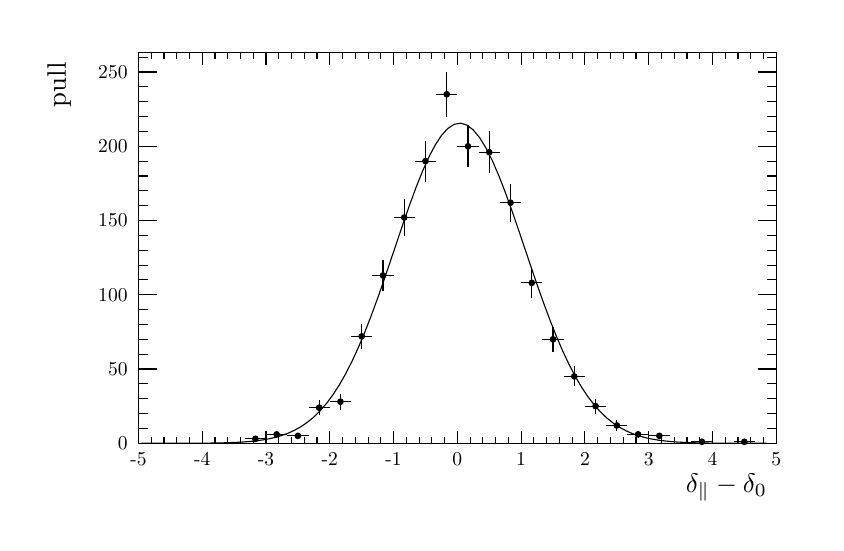
\begin{tikzpicture}
\pgfdeclareplotmark{cross} {
\pgfpathmoveto{\pgfpoint{-0.3\pgfplotmarksize}{\pgfplotmarksize}}
\pgfpathlineto{\pgfpoint{+0.3\pgfplotmarksize}{\pgfplotmarksize}}
\pgfpathlineto{\pgfpoint{+0.3\pgfplotmarksize}{0.3\pgfplotmarksize}}
\pgfpathlineto{\pgfpoint{+1\pgfplotmarksize}{0.3\pgfplotmarksize}}
\pgfpathlineto{\pgfpoint{+1\pgfplotmarksize}{-0.3\pgfplotmarksize}}
\pgfpathlineto{\pgfpoint{+0.3\pgfplotmarksize}{-0.3\pgfplotmarksize}}
\pgfpathlineto{\pgfpoint{+0.3\pgfplotmarksize}{-1.\pgfplotmarksize}}
\pgfpathlineto{\pgfpoint{-0.3\pgfplotmarksize}{-1.\pgfplotmarksize}}
\pgfpathlineto{\pgfpoint{-0.3\pgfplotmarksize}{-0.3\pgfplotmarksize}}
\pgfpathlineto{\pgfpoint{-1.\pgfplotmarksize}{-0.3\pgfplotmarksize}}
\pgfpathlineto{\pgfpoint{-1.\pgfplotmarksize}{0.3\pgfplotmarksize}}
\pgfpathlineto{\pgfpoint{-0.3\pgfplotmarksize}{0.3\pgfplotmarksize}}
\pgfpathclose
\pgfusepathqstroke
}
\pgfdeclareplotmark{cross*} {
\pgfpathmoveto{\pgfpoint{-0.3\pgfplotmarksize}{\pgfplotmarksize}}
\pgfpathlineto{\pgfpoint{+0.3\pgfplotmarksize}{\pgfplotmarksize}}
\pgfpathlineto{\pgfpoint{+0.3\pgfplotmarksize}{0.3\pgfplotmarksize}}
\pgfpathlineto{\pgfpoint{+1\pgfplotmarksize}{0.3\pgfplotmarksize}}
\pgfpathlineto{\pgfpoint{+1\pgfplotmarksize}{-0.3\pgfplotmarksize}}
\pgfpathlineto{\pgfpoint{+0.3\pgfplotmarksize}{-0.3\pgfplotmarksize}}
\pgfpathlineto{\pgfpoint{+0.3\pgfplotmarksize}{-1.\pgfplotmarksize}}
\pgfpathlineto{\pgfpoint{-0.3\pgfplotmarksize}{-1.\pgfplotmarksize}}
\pgfpathlineto{\pgfpoint{-0.3\pgfplotmarksize}{-0.3\pgfplotmarksize}}
\pgfpathlineto{\pgfpoint{-1.\pgfplotmarksize}{-0.3\pgfplotmarksize}}
\pgfpathlineto{\pgfpoint{-1.\pgfplotmarksize}{0.3\pgfplotmarksize}}
\pgfpathlineto{\pgfpoint{-0.3\pgfplotmarksize}{0.3\pgfplotmarksize}}
\pgfpathclose
\pgfusepathqfillstroke
}
\pgfdeclareplotmark{newstar} {
\pgfpathmoveto{\pgfqpoint{0pt}{\pgfplotmarksize}}
\pgfpathlineto{\pgfqpointpolar{44}{0.5\pgfplotmarksize}}
\pgfpathlineto{\pgfqpointpolar{18}{\pgfplotmarksize}}
\pgfpathlineto{\pgfqpointpolar{-20}{0.5\pgfplotmarksize}}
\pgfpathlineto{\pgfqpointpolar{-54}{\pgfplotmarksize}}
\pgfpathlineto{\pgfqpointpolar{-90}{0.5\pgfplotmarksize}}
\pgfpathlineto{\pgfqpointpolar{234}{\pgfplotmarksize}}
\pgfpathlineto{\pgfqpointpolar{198}{0.5\pgfplotmarksize}}
\pgfpathlineto{\pgfqpointpolar{162}{\pgfplotmarksize}}
\pgfpathlineto{\pgfqpointpolar{134}{0.5\pgfplotmarksize}}
\pgfpathclose
\pgfusepathqstroke
}
\pgfdeclareplotmark{newstar*} {
\pgfpathmoveto{\pgfqpoint{0pt}{\pgfplotmarksize}}
\pgfpathlineto{\pgfqpointpolar{44}{0.5\pgfplotmarksize}}
\pgfpathlineto{\pgfqpointpolar{18}{\pgfplotmarksize}}
\pgfpathlineto{\pgfqpointpolar{-20}{0.5\pgfplotmarksize}}
\pgfpathlineto{\pgfqpointpolar{-54}{\pgfplotmarksize}}
\pgfpathlineto{\pgfqpointpolar{-90}{0.5\pgfplotmarksize}}
\pgfpathlineto{\pgfqpointpolar{234}{\pgfplotmarksize}}
\pgfpathlineto{\pgfqpointpolar{198}{0.5\pgfplotmarksize}}
\pgfpathlineto{\pgfqpointpolar{162}{\pgfplotmarksize}}
\pgfpathlineto{\pgfqpointpolar{134}{0.5\pgfplotmarksize}}
\pgfpathclose
\pgfusepathqfillstroke
}
\definecolor{c}{rgb}{1,1,1};
\draw [color=c, fill=c] (0,0) rectangle (10,6.27517);
\draw [color=c, fill=c] (1.4,1.00403) rectangle (9.5,5.96141);
\definecolor{c}{rgb}{0,0,0};
\draw [c] (1.4,1.00403) -- (1.4,5.96141) -- (9.5,5.96141) -- (9.5,1.00403) -- (1.4,1.00403);
\draw [c] (2.885,1.02794) -- (2.885,1.06061);
\draw [c] (2.885,1.06061) -- (2.885,1.09328);
\draw [c] (2.75,1.06061) -- (2.885,1.06061);
\draw [c] (2.885,1.06061) -- (3.02,1.06061);
\foreach \P in {(2.885,1.06061)}{\draw[mark options={color=c,fill=c},mark size=2.402402pt,mark=*,mark size=1pt] plot coordinates {\P};}
\draw [c] (3.155,1.07099) -- (3.155,1.11719);
\draw [c] (3.155,1.11719) -- (3.155,1.16339);
\draw [c] (3.02,1.11719) -- (3.155,1.11719);
\draw [c] (3.155,1.11719) -- (3.29,1.11719);
\foreach \P in {(3.155,1.11719)}{\draw[mark options={color=c,fill=c},mark size=2.402402pt,mark=*,mark size=1pt] plot coordinates {\P};}
\draw [c] (3.425,1.05616) -- (3.425,1.09833);
\draw [c] (3.425,1.09833) -- (3.425,1.1405);
\draw [c] (3.29,1.09833) -- (3.425,1.09833);
\draw [c] (3.425,1.09833) -- (3.56,1.09833);
\foreach \P in {(3.425,1.09833)}{\draw[mark options={color=c,fill=c},mark size=2.402402pt,mark=*,mark size=1pt] plot coordinates {\P};}
\draw [c] (3.695,1.36428) -- (3.695,1.45668);
\draw [c] (3.695,1.45668) -- (3.695,1.54907);
\draw [c] (3.56,1.45668) -- (3.695,1.45668);
\draw [c] (3.695,1.45668) -- (3.83,1.45668);
\foreach \P in {(3.695,1.45668)}{\draw[mark options={color=c,fill=c},mark size=2.402402pt,mark=*,mark size=1pt] plot coordinates {\P};}
\draw [c] (3.965,1.43232) -- (3.965,1.53212);
\draw [c] (3.965,1.53212) -- (3.965,1.63192);
\draw [c] (3.83,1.53212) -- (3.965,1.53212);
\draw [c] (3.965,1.53212) -- (4.1,1.53212);
\foreach \P in {(3.965,1.53212)}{\draw[mark options={color=c,fill=c},mark size=2.402402pt,mark=*,mark size=1pt] plot coordinates {\P};}
\draw [c] (4.235,2.20194) -- (4.235,2.36198);
\draw [c] (4.235,2.36198) -- (4.235,2.52201);
\draw [c] (4.1,2.36198) -- (4.235,2.36198);
\draw [c] (4.235,2.36198) -- (4.37,2.36198);
\foreach \P in {(4.235,2.36198)}{\draw[mark options={color=c,fill=c},mark size=2.402402pt,mark=*,mark size=1pt] plot coordinates {\P};}
\draw [c] (4.505,2.93476) -- (4.505,3.13525);
\draw [c] (4.505,3.13525) -- (4.505,3.33574);
\draw [c] (4.37,3.13525) -- (4.505,3.13525);
\draw [c] (4.505,3.13525) -- (4.64,3.13525);
\foreach \P in {(4.505,3.13525)}{\draw[mark options={color=c,fill=c},mark size=2.402402pt,mark=*,mark size=1pt] plot coordinates {\P};}
\draw [c] (4.775,3.63828) -- (4.775,3.87081);
\draw [c] (4.775,3.87081) -- (4.775,4.10333);
\draw [c] (4.64,3.87081) -- (4.775,3.87081);
\draw [c] (4.775,3.87081) -- (4.91,3.87081);
\foreach \P in {(4.775,3.87081)}{\draw[mark options={color=c,fill=c},mark size=2.402402pt,mark=*,mark size=1pt] plot coordinates {\P};}
\draw [c] (5.045,4.32753) -- (5.045,4.5875);
\draw [c] (5.045,4.5875) -- (5.045,4.84747);
\draw [c] (4.91,4.5875) -- (5.045,4.5875);
\draw [c] (5.045,4.5875) -- (5.18,4.5875);
\foreach \P in {(5.045,4.5875)}{\draw[mark options={color=c,fill=c},mark size=2.402402pt,mark=*,mark size=1pt] plot coordinates {\P};}
\draw [c] (5.315,5.1471) -- (5.315,5.43622);
\draw [c] (5.315,5.43622) -- (5.315,5.72534);
\draw [c] (5.18,5.43622) -- (5.315,5.43622);
\draw [c] (5.315,5.43622) -- (5.45,5.43622);
\foreach \P in {(5.315,5.43622)}{\draw[mark options={color=c,fill=c},mark size=2.402402pt,mark=*,mark size=1pt] plot coordinates {\P};}
\draw [c] (5.585,4.50938) -- (5.585,4.77611);
\draw [c] (5.585,4.77611) -- (5.585,5.04283);
\draw [c] (5.45,4.77611) -- (5.585,4.77611);
\draw [c] (5.585,4.77611) -- (5.72,4.77611);
\foreach \P in {(5.585,4.77611)}{\draw[mark options={color=c,fill=c},mark size=2.402402pt,mark=*,mark size=1pt] plot coordinates {\P};}
\draw [c] (5.855,4.43662) -- (5.855,4.70066);
\draw [c] (5.855,4.70066) -- (5.855,4.96471);
\draw [c] (5.72,4.70066) -- (5.855,4.70066);
\draw [c] (5.855,4.70066) -- (5.99,4.70066);
\foreach \P in {(5.855,4.70066)}{\draw[mark options={color=c,fill=c},mark size=2.402402pt,mark=*,mark size=1pt] plot coordinates {\P};}
\draw [c] (6.125,3.81936) -- (6.125,4.05941);
\draw [c] (6.125,4.05941) -- (6.125,4.29946);
\draw [c] (5.99,4.05941) -- (6.125,4.05941);
\draw [c] (6.125,4.05941) -- (6.26,4.05941);
\foreach \P in {(6.125,4.05941)}{\draw[mark options={color=c,fill=c},mark size=2.402402pt,mark=*,mark size=1pt] plot coordinates {\P};}
\draw [c] (6.395,2.84495) -- (6.395,3.04095);
\draw [c] (6.395,3.04095) -- (6.395,3.23695);
\draw [c] (6.26,3.04095) -- (6.395,3.04095);
\draw [c] (6.395,3.04095) -- (6.53,3.04095);
\foreach \P in {(6.395,3.04095)}{\draw[mark options={color=c,fill=c},mark size=2.402402pt,mark=*,mark size=1pt] plot coordinates {\P};}
\draw [c] (6.665,2.16646) -- (6.665,2.32425);
\draw [c] (6.665,2.32425) -- (6.665,2.48205);
\draw [c] (6.53,2.32425) -- (6.665,2.32425);
\draw [c] (6.665,2.32425) -- (6.8,2.32425);
\foreach \P in {(6.665,2.32425)}{\draw[mark options={color=c,fill=c},mark size=2.402402pt,mark=*,mark size=1pt] plot coordinates {\P};}
\draw [c] (6.935,1.72623) -- (6.935,1.85274);
\draw [c] (6.935,1.85274) -- (6.935,1.97926);
\draw [c] (6.8,1.85274) -- (6.935,1.85274);
\draw [c] (6.935,1.85274) -- (7.07,1.85274);
\foreach \P in {(6.935,1.85274)}{\draw[mark options={color=c,fill=c},mark size=2.402402pt,mark=*,mark size=1pt] plot coordinates {\P};}
\draw [c] (7.205,1.38123) -- (7.205,1.47554);
\draw [c] (7.205,1.47554) -- (7.205,1.56984);
\draw [c] (7.07,1.47554) -- (7.205,1.47554);
\draw [c] (7.205,1.47554) -- (7.34,1.47554);
\foreach \P in {(7.205,1.47554)}{\draw[mark options={color=c,fill=c},mark size=2.402402pt,mark=*,mark size=1pt] plot coordinates {\P};}
\draw [c] (7.475,1.16502) -- (7.475,1.23035);
\draw [c] (7.475,1.23035) -- (7.475,1.29569);
\draw [c] (7.34,1.23035) -- (7.475,1.23035);
\draw [c] (7.475,1.23035) -- (7.61,1.23035);
\foreach \P in {(7.475,1.23035)}{\draw[mark options={color=c,fill=c},mark size=2.402402pt,mark=*,mark size=1pt] plot coordinates {\P};}
\draw [c] (7.745,1.07099) -- (7.745,1.11719);
\draw [c] (7.745,1.11719) -- (7.745,1.16339);
\draw [c] (7.61,1.11719) -- (7.745,1.11719);
\draw [c] (7.745,1.11719) -- (7.88,1.11719);
\foreach \P in {(7.745,1.11719)}{\draw[mark options={color=c,fill=c},mark size=2.402402pt,mark=*,mark size=1pt] plot coordinates {\P};}
\draw [c] (8.015,1.05616) -- (8.015,1.09833);
\draw [c] (8.015,1.09833) -- (8.015,1.1405);
\draw [c] (7.88,1.09833) -- (8.015,1.09833);
\draw [c] (8.015,1.09833) -- (8.15,1.09833);
\foreach \P in {(8.015,1.09833)}{\draw[mark options={color=c,fill=c},mark size=2.402402pt,mark=*,mark size=1pt] plot coordinates {\P};}
\draw [c] (8.555,1.00403) -- (8.555,1.02289);
\draw [c] (8.555,1.02289) -- (8.555,1.04175);
\draw [c] (8.42,1.02289) -- (8.555,1.02289);
\draw [c] (8.555,1.02289) -- (8.69,1.02289);
\foreach \P in {(8.555,1.02289)}{\draw[mark options={color=c,fill=c},mark size=2.402402pt,mark=*,mark size=1pt] plot coordinates {\P};}
\draw [c] (9.095,1.00403) -- (9.095,1.02289);
\draw [c] (9.095,1.02289) -- (9.095,1.04175);
\draw [c] (8.96,1.02289) -- (9.095,1.02289);
\draw [c] (9.095,1.02289) -- (9.23,1.02289);
\foreach \P in {(9.095,1.02289)}{\draw[mark options={color=c,fill=c},mark size=2.402402pt,mark=*,mark size=1pt] plot coordinates {\P};}
\draw [c,line width=0.4] (1.4405,1.00403) -- (1.5215,1.00403) -- (1.6025,1.00403) -- (1.6835,1.00403) -- (1.7645,1.00403) -- (1.8455,1.00403) -- (1.9265,1.00403) -- (2.0075,1.00466) -- (2.0885,1.00497) -- (2.1695,1.00543) -- (2.2505,1.00608) --
 (2.3315,1.00702) -- (2.4125,1.00835) -- (2.4935,1.0102) -- (2.5745,1.01276) -- (2.6555,1.01627) -- (2.7365,1.02102) -- (2.8175,1.0274) -- (2.8985,1.03586) -- (2.9795,1.04698) -- (3.0605,1.06143) -- (3.1415,1.08001) -- (3.2225,1.10365) --
 (3.3035,1.13341) -- (3.3845,1.17045) -- (3.4655,1.21607) -- (3.5465,1.27163) -- (3.6275,1.33853) -- (3.7085,1.41819) -- (3.7895,1.51194) -- (3.8705,1.62099) -- (3.9515,1.74635) -- (4.0325,1.88868) -- (4.1135,2.04829) -- (4.1945,2.22498) --
 (4.2755,2.41801) -- (4.3565,2.626) -- (4.4375,2.8469) -- (4.5185,3.07799) -- (4.5995,3.31589) -- (4.6805,3.55659) -- (4.7615,3.79557) -- (4.8425,4.02792) -- (4.9235,4.24849) -- (5.0045,4.45207) -- (5.0855,4.63361) -- (5.1665,4.7884) --
 (5.2475,4.91231) -- (5.3285,5.00193) -- (5.4095,5.05474);
\draw [c,line width=0.4] (5.4095,5.05474) -- (5.4905,5.06926) -- (5.5715,5.04506) -- (5.6525,4.98285) -- (5.7335,4.88437) -- (5.8145,4.75237) -- (5.8955,4.59046) -- (5.9765,4.40294) -- (6.0575,4.19462) -- (6.1385,3.97061) -- (6.2195,3.73612) --
 (6.3005,3.49626) -- (6.3815,3.25586) -- (6.4625,3.01932) -- (6.5435,2.79048) -- (6.6245,2.57259) -- (6.7055,2.36818) -- (6.7865,2.17914) -- (6.8675,2.00668) -- (6.9485,1.8514) -- (7.0295,1.71337) -- (7.1105,1.59218) -- (7.1915,1.48706) --
 (7.2725,1.39696) -- (7.3535,1.32063) -- (7.4345,1.2567) -- (7.5155,1.20376) -- (7.5965,1.16042) -- (7.6775,1.12532) -- (7.7585,1.0972) -- (7.8395,1.07492) -- (7.9205,1.05746) -- (8.0015,1.04391) -- (8.0825,1.03352) -- (8.1635,1.02563) --
 (8.2445,1.01969) -- (8.3255,1.01528) -- (8.4065,1.01204) -- (8.4875,1.00967) -- (8.5685,1.00797) -- (8.6495,1.00675) -- (8.7305,1.0059) -- (8.8115,1.00529) -- (8.8925,1.00488) -- (8.9735,1.00459) -- (9.0545,1.00403) -- (9.1355,1.00403) --
 (9.2165,1.00403) -- (9.2975,1.00403) -- (9.3785,1.00403);
\draw [c,line width=0.4] (9.3785,1.00403) -- (9.4595,1.00403);
\draw [c,line width=0.4] (1.4,1.00403) -- (9.5,1.00403);
\draw [anchor= east] (9.5,0.441772) node[scale=0.96888, rotate=0]{$\delta_\parallel-\delta_0$};
\draw [c,line width=0.4] (1.4,1.15651) -- (1.4,1.00403);
\draw [c,line width=0.4] (1.562,1.08027) -- (1.562,1.00403);
\draw [c,line width=0.4] (1.724,1.08027) -- (1.724,1.00403);
\draw [c,line width=0.4] (1.886,1.08027) -- (1.886,1.00403);
\draw [c,line width=0.4] (2.048,1.08027) -- (2.048,1.00403);
\draw [c,line width=0.4] (2.21,1.15651) -- (2.21,1.00403);
\draw [c,line width=0.4] (2.372,1.08027) -- (2.372,1.00403);
\draw [c,line width=0.4] (2.534,1.08027) -- (2.534,1.00403);
\draw [c,line width=0.4] (2.696,1.08027) -- (2.696,1.00403);
\draw [c,line width=0.4] (2.858,1.08027) -- (2.858,1.00403);
\draw [c,line width=0.4] (3.02,1.15651) -- (3.02,1.00403);
\draw [c,line width=0.4] (3.182,1.08027) -- (3.182,1.00403);
\draw [c,line width=0.4] (3.344,1.08027) -- (3.344,1.00403);
\draw [c,line width=0.4] (3.506,1.08027) -- (3.506,1.00403);
\draw [c,line width=0.4] (3.668,1.08027) -- (3.668,1.00403);
\draw [c,line width=0.4] (3.83,1.15651) -- (3.83,1.00403);
\draw [c,line width=0.4] (3.992,1.08027) -- (3.992,1.00403);
\draw [c,line width=0.4] (4.154,1.08027) -- (4.154,1.00403);
\draw [c,line width=0.4] (4.316,1.08027) -- (4.316,1.00403);
\draw [c,line width=0.4] (4.478,1.08027) -- (4.478,1.00403);
\draw [c,line width=0.4] (4.64,1.15651) -- (4.64,1.00403);
\draw [c,line width=0.4] (4.802,1.08027) -- (4.802,1.00403);
\draw [c,line width=0.4] (4.964,1.08027) -- (4.964,1.00403);
\draw [c,line width=0.4] (5.126,1.08027) -- (5.126,1.00403);
\draw [c,line width=0.4] (5.288,1.08027) -- (5.288,1.00403);
\draw [c,line width=0.4] (5.45,1.15651) -- (5.45,1.00403);
\draw [c,line width=0.4] (5.612,1.08027) -- (5.612,1.00403);
\draw [c,line width=0.4] (5.774,1.08027) -- (5.774,1.00403);
\draw [c,line width=0.4] (5.936,1.08027) -- (5.936,1.00403);
\draw [c,line width=0.4] (6.098,1.08027) -- (6.098,1.00403);
\draw [c,line width=0.4] (6.26,1.15651) -- (6.26,1.00403);
\draw [c,line width=0.4] (6.422,1.08027) -- (6.422,1.00403);
\draw [c,line width=0.4] (6.584,1.08027) -- (6.584,1.00403);
\draw [c,line width=0.4] (6.746,1.08027) -- (6.746,1.00403);
\draw [c,line width=0.4] (6.908,1.08027) -- (6.908,1.00403);
\draw [c,line width=0.4] (7.07,1.15651) -- (7.07,1.00403);
\draw [c,line width=0.4] (7.232,1.08027) -- (7.232,1.00403);
\draw [c,line width=0.4] (7.394,1.08027) -- (7.394,1.00403);
\draw [c,line width=0.4] (7.556,1.08027) -- (7.556,1.00403);
\draw [c,line width=0.4] (7.718,1.08027) -- (7.718,1.00403);
\draw [c,line width=0.4] (7.88,1.15651) -- (7.88,1.00403);
\draw [c,line width=0.4] (8.042,1.08027) -- (8.042,1.00403);
\draw [c,line width=0.4] (8.204,1.08027) -- (8.204,1.00403);
\draw [c,line width=0.4] (8.366,1.08027) -- (8.366,1.00403);
\draw [c,line width=0.4] (8.528,1.08027) -- (8.528,1.00403);
\draw [c,line width=0.4] (8.69,1.15651) -- (8.69,1.00403);
\draw [c,line width=0.4] (8.852,1.08027) -- (8.852,1.00403);
\draw [c,line width=0.4] (9.014,1.08027) -- (9.014,1.00403);
\draw [c,line width=0.4] (9.176,1.08027) -- (9.176,1.00403);
\draw [c,line width=0.4] (9.338,1.08027) -- (9.338,1.00403);
\draw [c,line width=0.4] (9.5,1.15651) -- (9.5,1.00403);
\draw [anchor=base] (1.4,0.721644) node[scale=0.708027, rotate=0]{-5};
\draw [anchor=base] (2.21,0.721644) node[scale=0.708027, rotate=0]{-4};
\draw [anchor=base] (3.02,0.721644) node[scale=0.708027, rotate=0]{-3};
\draw [anchor=base] (3.83,0.721644) node[scale=0.708027, rotate=0]{-2};
\draw [anchor=base] (4.64,0.721644) node[scale=0.708027, rotate=0]{-1};
\draw [anchor=base] (5.45,0.721644) node[scale=0.708027, rotate=0]{0};
\draw [anchor=base] (6.26,0.721644) node[scale=0.708027, rotate=0]{1};
\draw [anchor=base] (7.07,0.721644) node[scale=0.708027, rotate=0]{2};
\draw [anchor=base] (7.88,0.721644) node[scale=0.708027, rotate=0]{3};
\draw [anchor=base] (8.69,0.721644) node[scale=0.708027, rotate=0]{4};
\draw [anchor=base] (9.5,0.721644) node[scale=0.708027, rotate=0]{5};
\draw [c,line width=0.4] (1.4,5.96141) -- (9.5,5.96141);
\draw [c,line width=0.4] (1.4,5.80892) -- (1.4,5.96141);
\draw [c,line width=0.4] (1.562,5.88517) -- (1.562,5.96141);
\draw [c,line width=0.4] (1.724,5.88517) -- (1.724,5.96141);
\draw [c,line width=0.4] (1.886,5.88517) -- (1.886,5.96141);
\draw [c,line width=0.4] (2.048,5.88517) -- (2.048,5.96141);
\draw [c,line width=0.4] (2.21,5.80892) -- (2.21,5.96141);
\draw [c,line width=0.4] (2.372,5.88517) -- (2.372,5.96141);
\draw [c,line width=0.4] (2.534,5.88517) -- (2.534,5.96141);
\draw [c,line width=0.4] (2.696,5.88517) -- (2.696,5.96141);
\draw [c,line width=0.4] (2.858,5.88517) -- (2.858,5.96141);
\draw [c,line width=0.4] (3.02,5.80892) -- (3.02,5.96141);
\draw [c,line width=0.4] (3.182,5.88517) -- (3.182,5.96141);
\draw [c,line width=0.4] (3.344,5.88517) -- (3.344,5.96141);
\draw [c,line width=0.4] (3.506,5.88517) -- (3.506,5.96141);
\draw [c,line width=0.4] (3.668,5.88517) -- (3.668,5.96141);
\draw [c,line width=0.4] (3.83,5.80892) -- (3.83,5.96141);
\draw [c,line width=0.4] (3.992,5.88517) -- (3.992,5.96141);
\draw [c,line width=0.4] (4.154,5.88517) -- (4.154,5.96141);
\draw [c,line width=0.4] (4.316,5.88517) -- (4.316,5.96141);
\draw [c,line width=0.4] (4.478,5.88517) -- (4.478,5.96141);
\draw [c,line width=0.4] (4.64,5.80892) -- (4.64,5.96141);
\draw [c,line width=0.4] (4.802,5.88517) -- (4.802,5.96141);
\draw [c,line width=0.4] (4.964,5.88517) -- (4.964,5.96141);
\draw [c,line width=0.4] (5.126,5.88517) -- (5.126,5.96141);
\draw [c,line width=0.4] (5.288,5.88517) -- (5.288,5.96141);
\draw [c,line width=0.4] (5.45,5.80892) -- (5.45,5.96141);
\draw [c,line width=0.4] (5.612,5.88517) -- (5.612,5.96141);
\draw [c,line width=0.4] (5.774,5.88517) -- (5.774,5.96141);
\draw [c,line width=0.4] (5.936,5.88517) -- (5.936,5.96141);
\draw [c,line width=0.4] (6.098,5.88517) -- (6.098,5.96141);
\draw [c,line width=0.4] (6.26,5.80892) -- (6.26,5.96141);
\draw [c,line width=0.4] (6.422,5.88517) -- (6.422,5.96141);
\draw [c,line width=0.4] (6.584,5.88517) -- (6.584,5.96141);
\draw [c,line width=0.4] (6.746,5.88517) -- (6.746,5.96141);
\draw [c,line width=0.4] (6.908,5.88517) -- (6.908,5.96141);
\draw [c,line width=0.4] (7.07,5.80892) -- (7.07,5.96141);
\draw [c,line width=0.4] (7.232,5.88517) -- (7.232,5.96141);
\draw [c,line width=0.4] (7.394,5.88517) -- (7.394,5.96141);
\draw [c,line width=0.4] (7.556,5.88517) -- (7.556,5.96141);
\draw [c,line width=0.4] (7.718,5.88517) -- (7.718,5.96141);
\draw [c,line width=0.4] (7.88,5.80892) -- (7.88,5.96141);
\draw [c,line width=0.4] (8.042,5.88517) -- (8.042,5.96141);
\draw [c,line width=0.4] (8.204,5.88517) -- (8.204,5.96141);
\draw [c,line width=0.4] (8.366,5.88517) -- (8.366,5.96141);
\draw [c,line width=0.4] (8.528,5.88517) -- (8.528,5.96141);
\draw [c,line width=0.4] (8.69,5.80892) -- (8.69,5.96141);
\draw [c,line width=0.4] (8.852,5.88517) -- (8.852,5.96141);
\draw [c,line width=0.4] (9.014,5.88517) -- (9.014,5.96141);
\draw [c,line width=0.4] (9.176,5.88517) -- (9.176,5.96141);
\draw [c,line width=0.4] (9.338,5.88517) -- (9.338,5.96141);
\draw [c,line width=0.4] (9.5,5.80892) -- (9.5,5.96141);
\draw [c,line width=0.4] (1.4,1.00403) -- (1.4,5.96141);
\draw [anchor= east] (0.392,5.96141) node[scale=0.96888, rotate=90]{pull};
\draw [c,line width=0.4] (1.637,1.00403) -- (1.4,1.00403);
\draw [c,line width=0.4] (1.5185,1.19263) -- (1.4,1.19263);
\draw [c,line width=0.4] (1.5185,1.38123) -- (1.4,1.38123);
\draw [c,line width=0.4] (1.5185,1.56984) -- (1.4,1.56984);
\draw [c,line width=0.4] (1.5185,1.75844) -- (1.4,1.75844);
\draw [c,line width=0.4] (1.637,1.94705) -- (1.4,1.94705);
\draw [c,line width=0.4] (1.5185,2.13565) -- (1.4,2.13565);
\draw [c,line width=0.4] (1.5185,2.32425) -- (1.4,2.32425);
\draw [c,line width=0.4] (1.5185,2.51286) -- (1.4,2.51286);
\draw [c,line width=0.4] (1.5185,2.70146) -- (1.4,2.70146);
\draw [c,line width=0.4] (1.637,2.89007) -- (1.4,2.89007);
\draw [c,line width=0.4] (1.5185,3.07867) -- (1.4,3.07867);
\draw [c,line width=0.4] (1.5185,3.26727) -- (1.4,3.26727);
\draw [c,line width=0.4] (1.5185,3.45588) -- (1.4,3.45588);
\draw [c,line width=0.4] (1.5185,3.64448) -- (1.4,3.64448);
\draw [c,line width=0.4] (1.637,3.83309) -- (1.4,3.83309);
\draw [c,line width=0.4] (1.5185,4.02169) -- (1.4,4.02169);
\draw [c,line width=0.4] (1.5185,4.21029) -- (1.4,4.21029);
\draw [c,line width=0.4] (1.5185,4.3989) -- (1.4,4.3989);
\draw [c,line width=0.4] (1.5185,4.5875) -- (1.4,4.5875);
\draw [c,line width=0.4] (1.637,4.77611) -- (1.4,4.77611);
\draw [c,line width=0.4] (1.5185,4.96471) -- (1.4,4.96471);
\draw [c,line width=0.4] (1.5185,5.15331) -- (1.4,5.15331);
\draw [c,line width=0.4] (1.5185,5.34192) -- (1.4,5.34192);
\draw [c,line width=0.4] (1.5185,5.53052) -- (1.4,5.53052);
\draw [c,line width=0.4] (1.637,5.71913) -- (1.4,5.71913);
\draw [c,line width=0.4] (1.637,5.71913) -- (1.4,5.71913);
\draw [c,line width=0.4] (1.5185,5.90773) -- (1.4,5.90773);
\draw [anchor= east] (1.35,1.00403) node[scale=0.708027, rotate=0]{0};
\draw [anchor= east] (1.35,1.94705) node[scale=0.708027, rotate=0]{50};
\draw [anchor= east] (1.35,2.89007) node[scale=0.708027, rotate=0]{100};
\draw [anchor= east] (1.35,3.83309) node[scale=0.708027, rotate=0]{150};
\draw [anchor= east] (1.35,4.77611) node[scale=0.708027, rotate=0]{200};
\draw [anchor= east] (1.35,5.71913) node[scale=0.708027, rotate=0]{250};
\draw [c,line width=0.4] (9.5,1.00403) -- (9.5,5.96141);
\draw [c,line width=0.4] (9.263,1.00403) -- (9.5,1.00403);
\draw [c,line width=0.4] (9.3815,1.19263) -- (9.5,1.19263);
\draw [c,line width=0.4] (9.3815,1.38123) -- (9.5,1.38123);
\draw [c,line width=0.4] (9.3815,1.56984) -- (9.5,1.56984);
\draw [c,line width=0.4] (9.3815,1.75844) -- (9.5,1.75844);
\draw [c,line width=0.4] (9.263,1.94705) -- (9.5,1.94705);
\draw [c,line width=0.4] (9.3815,2.13565) -- (9.5,2.13565);
\draw [c,line width=0.4] (9.3815,2.32425) -- (9.5,2.32425);
\draw [c,line width=0.4] (9.3815,2.51286) -- (9.5,2.51286);
\draw [c,line width=0.4] (9.3815,2.70146) -- (9.5,2.70146);
\draw [c,line width=0.4] (9.263,2.89007) -- (9.5,2.89007);
\draw [c,line width=0.4] (9.3815,3.07867) -- (9.5,3.07867);
\draw [c,line width=0.4] (9.3815,3.26727) -- (9.5,3.26727);
\draw [c,line width=0.4] (9.3815,3.45588) -- (9.5,3.45588);
\draw [c,line width=0.4] (9.3815,3.64448) -- (9.5,3.64448);
\draw [c,line width=0.4] (9.263,3.83309) -- (9.5,3.83309);
\draw [c,line width=0.4] (9.3815,4.02169) -- (9.5,4.02169);
\draw [c,line width=0.4] (9.3815,4.21029) -- (9.5,4.21029);
\draw [c,line width=0.4] (9.3815,4.3989) -- (9.5,4.3989);
\draw [c,line width=0.4] (9.3815,4.5875) -- (9.5,4.5875);
\draw [c,line width=0.4] (9.263,4.77611) -- (9.5,4.77611);
\draw [c,line width=0.4] (9.3815,4.96471) -- (9.5,4.96471);
\draw [c,line width=0.4] (9.3815,5.15331) -- (9.5,5.15331);
\draw [c,line width=0.4] (9.3815,5.34192) -- (9.5,5.34192);
\draw [c,line width=0.4] (9.3815,5.53052) -- (9.5,5.53052);
\draw [c,line width=0.4] (9.263,5.71913) -- (9.5,5.71913);
\draw [c,line width=0.4] (9.263,5.71913) -- (9.5,5.71913);
\draw [c,line width=0.4] (9.3815,5.90773) -- (9.5,5.90773);
\end{tikzpicture}
}
    \caption{}
    \label{pull_AparPhase}
  \end{subfigure}%
  \hfill%
  \begin{subfigure}{0.5\textwidth}
    \tikzsetnextfilename{pull_AperpPhase} 
    \scalebox{0.60}{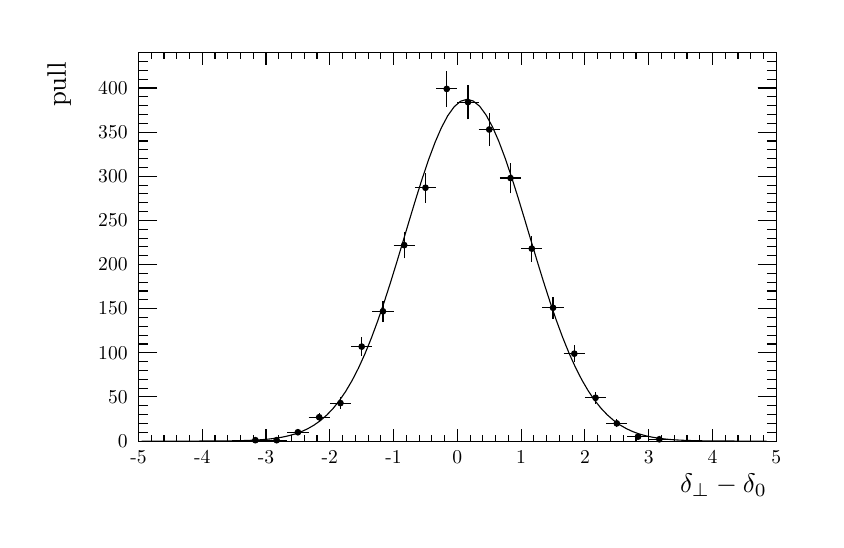
\begin{tikzpicture}
\pgfdeclareplotmark{cross} {
\pgfpathmoveto{\pgfpoint{-0.3\pgfplotmarksize}{\pgfplotmarksize}}
\pgfpathlineto{\pgfpoint{+0.3\pgfplotmarksize}{\pgfplotmarksize}}
\pgfpathlineto{\pgfpoint{+0.3\pgfplotmarksize}{0.3\pgfplotmarksize}}
\pgfpathlineto{\pgfpoint{+1\pgfplotmarksize}{0.3\pgfplotmarksize}}
\pgfpathlineto{\pgfpoint{+1\pgfplotmarksize}{-0.3\pgfplotmarksize}}
\pgfpathlineto{\pgfpoint{+0.3\pgfplotmarksize}{-0.3\pgfplotmarksize}}
\pgfpathlineto{\pgfpoint{+0.3\pgfplotmarksize}{-1.\pgfplotmarksize}}
\pgfpathlineto{\pgfpoint{-0.3\pgfplotmarksize}{-1.\pgfplotmarksize}}
\pgfpathlineto{\pgfpoint{-0.3\pgfplotmarksize}{-0.3\pgfplotmarksize}}
\pgfpathlineto{\pgfpoint{-1.\pgfplotmarksize}{-0.3\pgfplotmarksize}}
\pgfpathlineto{\pgfpoint{-1.\pgfplotmarksize}{0.3\pgfplotmarksize}}
\pgfpathlineto{\pgfpoint{-0.3\pgfplotmarksize}{0.3\pgfplotmarksize}}
\pgfpathclose
\pgfusepathqstroke
}
\pgfdeclareplotmark{cross*} {
\pgfpathmoveto{\pgfpoint{-0.3\pgfplotmarksize}{\pgfplotmarksize}}
\pgfpathlineto{\pgfpoint{+0.3\pgfplotmarksize}{\pgfplotmarksize}}
\pgfpathlineto{\pgfpoint{+0.3\pgfplotmarksize}{0.3\pgfplotmarksize}}
\pgfpathlineto{\pgfpoint{+1\pgfplotmarksize}{0.3\pgfplotmarksize}}
\pgfpathlineto{\pgfpoint{+1\pgfplotmarksize}{-0.3\pgfplotmarksize}}
\pgfpathlineto{\pgfpoint{+0.3\pgfplotmarksize}{-0.3\pgfplotmarksize}}
\pgfpathlineto{\pgfpoint{+0.3\pgfplotmarksize}{-1.\pgfplotmarksize}}
\pgfpathlineto{\pgfpoint{-0.3\pgfplotmarksize}{-1.\pgfplotmarksize}}
\pgfpathlineto{\pgfpoint{-0.3\pgfplotmarksize}{-0.3\pgfplotmarksize}}
\pgfpathlineto{\pgfpoint{-1.\pgfplotmarksize}{-0.3\pgfplotmarksize}}
\pgfpathlineto{\pgfpoint{-1.\pgfplotmarksize}{0.3\pgfplotmarksize}}
\pgfpathlineto{\pgfpoint{-0.3\pgfplotmarksize}{0.3\pgfplotmarksize}}
\pgfpathclose
\pgfusepathqfillstroke
}
\pgfdeclareplotmark{newstar} {
\pgfpathmoveto{\pgfqpoint{0pt}{\pgfplotmarksize}}
\pgfpathlineto{\pgfqpointpolar{44}{0.5\pgfplotmarksize}}
\pgfpathlineto{\pgfqpointpolar{18}{\pgfplotmarksize}}
\pgfpathlineto{\pgfqpointpolar{-20}{0.5\pgfplotmarksize}}
\pgfpathlineto{\pgfqpointpolar{-54}{\pgfplotmarksize}}
\pgfpathlineto{\pgfqpointpolar{-90}{0.5\pgfplotmarksize}}
\pgfpathlineto{\pgfqpointpolar{234}{\pgfplotmarksize}}
\pgfpathlineto{\pgfqpointpolar{198}{0.5\pgfplotmarksize}}
\pgfpathlineto{\pgfqpointpolar{162}{\pgfplotmarksize}}
\pgfpathlineto{\pgfqpointpolar{134}{0.5\pgfplotmarksize}}
\pgfpathclose
\pgfusepathqstroke
}
\pgfdeclareplotmark{newstar*} {
\pgfpathmoveto{\pgfqpoint{0pt}{\pgfplotmarksize}}
\pgfpathlineto{\pgfqpointpolar{44}{0.5\pgfplotmarksize}}
\pgfpathlineto{\pgfqpointpolar{18}{\pgfplotmarksize}}
\pgfpathlineto{\pgfqpointpolar{-20}{0.5\pgfplotmarksize}}
\pgfpathlineto{\pgfqpointpolar{-54}{\pgfplotmarksize}}
\pgfpathlineto{\pgfqpointpolar{-90}{0.5\pgfplotmarksize}}
\pgfpathlineto{\pgfqpointpolar{234}{\pgfplotmarksize}}
\pgfpathlineto{\pgfqpointpolar{198}{0.5\pgfplotmarksize}}
\pgfpathlineto{\pgfqpointpolar{162}{\pgfplotmarksize}}
\pgfpathlineto{\pgfqpointpolar{134}{0.5\pgfplotmarksize}}
\pgfpathclose
\pgfusepathqfillstroke
}
\definecolor{c}{rgb}{1,1,1};
\draw [color=c, fill=c] (0,0) rectangle (10,6.24161);
\draw [color=c, fill=c] (1.4,0.998658) rectangle (9.5,5.92953);
\definecolor{c}{rgb}{0,0,0};
\draw [c] (1.4,0.998658) -- (1.4,5.92953) -- (9.5,5.92953) -- (9.5,0.998658) -- (1.4,0.998658);
\draw [c] (2.885,0.998658) -- (2.885,1.00987);
\draw [c] (2.885,1.00987) -- (2.885,1.02107);
\draw [c] (2.75,1.00987) -- (2.885,1.00987);
\draw [c] (2.885,1.00987) -- (3.02,1.00987);
\foreach \P in {(2.885,1.00987)}{\draw[mark options={color=c,fill=c},mark size=2.402402pt,mark=*,mark size=1pt] plot coordinates {\P};}
\draw [c] (3.155,0.998658) -- (3.155,1.00987);
\draw [c] (3.155,1.00987) -- (3.155,1.02107);
\draw [c] (3.02,1.00987) -- (3.155,1.00987);
\draw [c] (3.155,1.00987) -- (3.29,1.00987);
\foreach \P in {(3.155,1.00987)}{\draw[mark options={color=c,fill=c},mark size=2.402402pt,mark=*,mark size=1pt] plot coordinates {\P};}
\draw [c] (3.425,1.0753) -- (3.425,1.11074);
\draw [c] (3.425,1.11074) -- (3.425,1.14619);
\draw [c] (3.29,1.11074) -- (3.425,1.11074);
\draw [c] (3.425,1.11074) -- (3.56,1.11074);
\foreach \P in {(3.425,1.11074)}{\draw[mark options={color=c,fill=c},mark size=2.402402pt,mark=*,mark size=1pt] plot coordinates {\P};}
\draw [c] (3.695,1.24305) -- (3.695,1.30129);
\draw [c] (3.695,1.30129) -- (3.695,1.35953);
\draw [c] (3.56,1.30129) -- (3.695,1.30129);
\draw [c] (3.695,1.30129) -- (3.83,1.30129);
\foreach \P in {(3.695,1.30129)}{\draw[mark options={color=c,fill=c},mark size=2.402402pt,mark=*,mark size=1pt] plot coordinates {\P};}
\draw [c] (3.965,1.40712) -- (3.965,1.48062);
\draw [c] (3.965,1.48062) -- (3.965,1.55412);
\draw [c] (3.83,1.48062) -- (3.965,1.48062);
\draw [c] (3.965,1.48062) -- (4.1,1.48062);
\foreach \P in {(3.965,1.48062)}{\draw[mark options={color=c,fill=c},mark size=2.402402pt,mark=*,mark size=1pt] plot coordinates {\P};}
\draw [c] (4.235,2.08202) -- (4.235,2.19796);
\draw [c] (4.235,2.19796) -- (4.235,2.31391);
\draw [c] (4.1,2.19796) -- (4.235,2.19796);
\draw [c] (4.235,2.19796) -- (4.37,2.19796);
\foreach \P in {(4.235,2.19796)}{\draw[mark options={color=c,fill=c},mark size=2.402402pt,mark=*,mark size=1pt] plot coordinates {\P};}
\draw [c] (4.505,2.51041) -- (4.505,2.6463);
\draw [c] (4.505,2.6463) -- (4.505,2.7822);
\draw [c] (4.37,2.6463) -- (4.505,2.6463);
\draw [c] (4.505,2.6463) -- (4.64,2.6463);
\foreach \P in {(4.505,2.6463)}{\draw[mark options={color=c,fill=c},mark size=2.402402pt,mark=*,mark size=1pt] plot coordinates {\P};}
\draw [c] (4.775,3.31994) -- (4.775,3.48694);
\draw [c] (4.775,3.48694) -- (4.775,3.65394);
\draw [c] (4.64,3.48694) -- (4.775,3.48694);
\draw [c] (4.775,3.48694) -- (4.91,3.48694);
\foreach \P in {(4.775,3.48694)}{\draw[mark options={color=c,fill=c},mark size=2.402402pt,mark=*,mark size=1pt] plot coordinates {\P};}
\draw [c] (5.045,4.02561) -- (5.045,4.21549);
\draw [c] (5.045,4.21549) -- (5.045,4.40537);
\draw [c] (4.91,4.21549) -- (5.045,4.21549);
\draw [c] (5.045,4.21549) -- (5.18,4.21549);
\foreach \P in {(5.045,4.21549)}{\draw[mark options={color=c,fill=c},mark size=2.402402pt,mark=*,mark size=1pt] plot coordinates {\P};}
\draw [c] (5.315,5.24695) -- (5.315,5.47084);
\draw [c] (5.315,5.47084) -- (5.315,5.69473);
\draw [c] (5.18,5.47084) -- (5.315,5.47084);
\draw [c] (5.315,5.47084) -- (5.45,5.47084);
\foreach \P in {(5.315,5.47084)}{\draw[mark options={color=c,fill=c},mark size=2.402402pt,mark=*,mark size=1pt] plot coordinates {\P};}
\draw [c] (5.585,5.08307) -- (5.585,5.30271);
\draw [c] (5.585,5.30271) -- (5.585,5.52235);
\draw [c] (5.45,5.30271) -- (5.585,5.30271);
\draw [c] (5.585,5.30271) -- (5.72,5.30271);
\foreach \P in {(5.585,5.30271)}{\draw[mark options={color=c,fill=c},mark size=2.402402pt,mark=*,mark size=1pt] plot coordinates {\P};}
\draw [c] (5.855,4.74466) -- (5.855,4.95525);
\draw [c] (5.855,4.95525) -- (5.855,5.16584);
\draw [c] (5.72,4.95525) -- (5.855,4.95525);
\draw [c] (5.855,4.95525) -- (5.99,4.95525);
\foreach \P in {(5.855,4.95525)}{\draw[mark options={color=c,fill=c},mark size=2.402402pt,mark=*,mark size=1pt] plot coordinates {\P};}
\draw [c] (6.125,4.14529) -- (6.125,4.33878);
\draw [c] (6.125,4.33878) -- (6.125,4.53227);
\draw [c] (5.99,4.33878) -- (6.125,4.33878);
\draw [c] (6.125,4.33878) -- (6.26,4.33878);
\foreach \P in {(6.125,4.33878)}{\draw[mark options={color=c,fill=c},mark size=2.402402pt,mark=*,mark size=1pt] plot coordinates {\P};}
\draw [c] (6.395,3.27661) -- (6.395,3.4421);
\draw [c] (6.395,3.4421) -- (6.395,3.6076);
\draw [c] (6.26,3.4421) -- (6.395,3.4421);
\draw [c] (6.395,3.4421) -- (6.53,3.4421);
\foreach \P in {(6.395,3.4421)}{\draw[mark options={color=c,fill=c},mark size=2.402402pt,mark=*,mark size=1pt] plot coordinates {\P};}
\draw [c] (6.665,2.5534) -- (6.665,2.69114);
\draw [c] (6.665,2.69114) -- (6.665,2.82887);
\draw [c] (6.53,2.69114) -- (6.665,2.69114);
\draw [c] (6.665,2.69114) -- (6.8,2.69114);
\foreach \P in {(6.665,2.69114)}{\draw[mark options={color=c,fill=c},mark size=2.402402pt,mark=*,mark size=1pt] plot coordinates {\P};}
\draw [c] (6.935,1.99677) -- (6.935,2.1083);
\draw [c] (6.935,2.1083) -- (6.935,2.21982);
\draw [c] (6.8,2.1083) -- (6.935,2.1083);
\draw [c] (6.935,2.1083) -- (7.07,2.1083);
\foreach \P in {(6.935,2.1083)}{\draw[mark options={color=c,fill=c},mark size=2.402402pt,mark=*,mark size=1pt] plot coordinates {\P};}
\draw [c] (7.205,1.46941) -- (7.205,1.54787);
\draw [c] (7.205,1.54787) -- (7.205,1.62633);
\draw [c] (7.07,1.54787) -- (7.205,1.54787);
\draw [c] (7.205,1.54787) -- (7.34,1.54787);
\foreach \P in {(7.205,1.54787)}{\draw[mark options={color=c,fill=c},mark size=2.402402pt,mark=*,mark size=1pt] plot coordinates {\P};}
\draw [c] (7.475,1.1727) -- (7.475,1.22283);
\draw [c] (7.475,1.22283) -- (7.475,1.27295);
\draw [c] (7.34,1.22283) -- (7.475,1.22283);
\draw [c] (7.475,1.22283) -- (7.61,1.22283);
\foreach \P in {(7.475,1.22283)}{\draw[mark options={color=c,fill=c},mark size=2.402402pt,mark=*,mark size=1pt] plot coordinates {\P};}
\draw [c] (7.745,1.02964) -- (7.745,1.0547);
\draw [c] (7.745,1.0547) -- (7.745,1.07976);
\draw [c] (7.61,1.0547) -- (7.745,1.0547);
\draw [c] (7.745,1.0547) -- (7.88,1.0547);
\foreach \P in {(7.745,1.0547)}{\draw[mark options={color=c,fill=c},mark size=2.402402pt,mark=*,mark size=1pt] plot coordinates {\P};}
\draw [c] (8.015,1.00522) -- (8.015,1.02107);
\draw [c] (8.015,1.02107) -- (8.015,1.03693);
\draw [c] (7.88,1.02107) -- (8.015,1.02107);
\draw [c] (8.015,1.02107) -- (8.15,1.02107);
\foreach \P in {(8.015,1.02107)}{\draw[mark options={color=c,fill=c},mark size=2.402402pt,mark=*,mark size=1pt] plot coordinates {\P};}
\draw [c,line width=0.4] (1.4405,0.998658) -- (1.5215,0.998658) -- (1.6025,0.998658) -- (1.6835,0.998658) -- (1.7645,0.998658) -- (1.8455,0.998658) -- (1.9265,0.998658) -- (2.0075,0.998658) -- (2.0885,0.998658) -- (2.1695,0.998658) --
 (2.2505,0.999218) -- (2.3315,0.99952) -- (2.4125,0.99997) -- (2.4935,1.00064) -- (2.5745,1.00161) -- (2.6555,1.00301) -- (2.7365,1.005) -- (2.8175,1.00782) -- (2.8985,1.01175) -- (2.9795,1.01716) -- (3.0605,1.02454) -- (3.1415,1.03447) --
 (3.2225,1.04769) -- (3.3035,1.06508) -- (3.3845,1.08768) -- (3.4655,1.11671) -- (3.5465,1.15355) -- (3.6275,1.19974) -- (3.7085,1.25693) -- (3.7895,1.32689) -- (3.8705,1.41138) -- (3.9515,1.51213) -- (4.0325,1.63071) -- (4.1135,1.76844) --
 (4.1945,1.92627) -- (4.2755,2.10463) -- (4.3565,2.30334) -- (4.4375,2.52145) -- (4.5185,2.75722) -- (4.5995,3.00801) -- (4.6805,3.27027) -- (4.7615,3.53958) -- (4.8425,3.81075) -- (4.9235,4.07792) -- (5.0045,4.3348) -- (5.0855,4.57487) --
 (5.1665,4.79164) -- (5.2475,4.97898) -- (5.3285,5.13138) -- (5.4095,5.24422);
\draw [c,line width=0.4] (5.4095,5.24422) -- (5.4905,5.31398) -- (5.5715,5.33847) -- (5.6525,5.31692) -- (5.7335,5.25001) -- (5.8145,5.13985) -- (5.8955,4.98986) -- (5.9765,4.8046) -- (6.0575,4.58954) -- (6.1385,4.35077) -- (6.2195,4.09478) --
 (6.3005,3.82807) -- (6.3815,3.55698) -- (6.4625,3.28738) -- (6.5435,3.02453) -- (6.6245,2.77289) -- (6.7055,2.53607) -- (6.7865,2.31676) -- (6.8675,2.11677) -- (6.9485,1.9371) -- (7.0295,1.77796) -- (7.1105,1.63896) -- (7.1915,1.51918) --
 (7.2725,1.41734) -- (7.3535,1.33185) -- (7.4345,1.26102) -- (7.5155,1.20306) -- (7.5965,1.15621) -- (7.6775,1.11882) -- (7.7585,1.08933) -- (7.8395,1.06636) -- (7.9205,1.04867) -- (8.0015,1.03521) -- (8.0825,1.02509) -- (8.1635,1.01757) --
 (8.2445,1.01205) -- (8.3255,1.00804) -- (8.4065,1.00516) -- (8.4875,1.00311) -- (8.5685,1.00168) -- (8.6495,1.00069) -- (8.7305,1.00001) -- (8.8115,0.999544) -- (8.8925,0.999234) -- (8.9735,0.998658) -- (9.0545,0.998658) -- (9.1355,0.998658) --
 (9.2165,0.998658) -- (9.2975,0.998658) -- (9.3785,0.998658);
\draw [c,line width=0.4] (9.3785,0.998658) -- (9.4595,0.998658);
\draw [c,line width=0.4] (1.4,0.998658) -- (9.5,0.998658);
\draw [anchor= east] (9.5,0.439409) node[scale=0.96888, rotate=0]{$\delta_\perp-\delta_0$};
\draw [c,line width=0.4] (1.4,1.15033) -- (1.4,0.998658);
\draw [c,line width=0.4] (1.562,1.07449) -- (1.562,0.998658);
\draw [c,line width=0.4] (1.724,1.07449) -- (1.724,0.998658);
\draw [c,line width=0.4] (1.886,1.07449) -- (1.886,0.998658);
\draw [c,line width=0.4] (2.048,1.07449) -- (2.048,0.998658);
\draw [c,line width=0.4] (2.21,1.15033) -- (2.21,0.998658);
\draw [c,line width=0.4] (2.372,1.07449) -- (2.372,0.998658);
\draw [c,line width=0.4] (2.534,1.07449) -- (2.534,0.998658);
\draw [c,line width=0.4] (2.696,1.07449) -- (2.696,0.998658);
\draw [c,line width=0.4] (2.858,1.07449) -- (2.858,0.998658);
\draw [c,line width=0.4] (3.02,1.15033) -- (3.02,0.998658);
\draw [c,line width=0.4] (3.182,1.07449) -- (3.182,0.998658);
\draw [c,line width=0.4] (3.344,1.07449) -- (3.344,0.998658);
\draw [c,line width=0.4] (3.506,1.07449) -- (3.506,0.998658);
\draw [c,line width=0.4] (3.668,1.07449) -- (3.668,0.998658);
\draw [c,line width=0.4] (3.83,1.15033) -- (3.83,0.998658);
\draw [c,line width=0.4] (3.992,1.07449) -- (3.992,0.998658);
\draw [c,line width=0.4] (4.154,1.07449) -- (4.154,0.998658);
\draw [c,line width=0.4] (4.316,1.07449) -- (4.316,0.998658);
\draw [c,line width=0.4] (4.478,1.07449) -- (4.478,0.998658);
\draw [c,line width=0.4] (4.64,1.15033) -- (4.64,0.998658);
\draw [c,line width=0.4] (4.802,1.07449) -- (4.802,0.998658);
\draw [c,line width=0.4] (4.964,1.07449) -- (4.964,0.998658);
\draw [c,line width=0.4] (5.126,1.07449) -- (5.126,0.998658);
\draw [c,line width=0.4] (5.288,1.07449) -- (5.288,0.998658);
\draw [c,line width=0.4] (5.45,1.15033) -- (5.45,0.998658);
\draw [c,line width=0.4] (5.612,1.07449) -- (5.612,0.998658);
\draw [c,line width=0.4] (5.774,1.07449) -- (5.774,0.998658);
\draw [c,line width=0.4] (5.936,1.07449) -- (5.936,0.998658);
\draw [c,line width=0.4] (6.098,1.07449) -- (6.098,0.998658);
\draw [c,line width=0.4] (6.26,1.15033) -- (6.26,0.998658);
\draw [c,line width=0.4] (6.422,1.07449) -- (6.422,0.998658);
\draw [c,line width=0.4] (6.584,1.07449) -- (6.584,0.998658);
\draw [c,line width=0.4] (6.746,1.07449) -- (6.746,0.998658);
\draw [c,line width=0.4] (6.908,1.07449) -- (6.908,0.998658);
\draw [c,line width=0.4] (7.07,1.15033) -- (7.07,0.998658);
\draw [c,line width=0.4] (7.232,1.07449) -- (7.232,0.998658);
\draw [c,line width=0.4] (7.394,1.07449) -- (7.394,0.998658);
\draw [c,line width=0.4] (7.556,1.07449) -- (7.556,0.998658);
\draw [c,line width=0.4] (7.718,1.07449) -- (7.718,0.998658);
\draw [c,line width=0.4] (7.88,1.15033) -- (7.88,0.998658);
\draw [c,line width=0.4] (8.042,1.07449) -- (8.042,0.998658);
\draw [c,line width=0.4] (8.204,1.07449) -- (8.204,0.998658);
\draw [c,line width=0.4] (8.366,1.07449) -- (8.366,0.998658);
\draw [c,line width=0.4] (8.528,1.07449) -- (8.528,0.998658);
\draw [c,line width=0.4] (8.69,1.15033) -- (8.69,0.998658);
\draw [c,line width=0.4] (8.852,1.07449) -- (8.852,0.998658);
\draw [c,line width=0.4] (9.014,1.07449) -- (9.014,0.998658);
\draw [c,line width=0.4] (9.176,1.07449) -- (9.176,0.998658);
\draw [c,line width=0.4] (9.338,1.07449) -- (9.338,0.998658);
\draw [c,line width=0.4] (9.5,1.15033) -- (9.5,0.998658);
\draw [anchor=base] (1.4,0.717785) node[scale=0.708027, rotate=0]{-5};
\draw [anchor=base] (2.21,0.717785) node[scale=0.708027, rotate=0]{-4};
\draw [anchor=base] (3.02,0.717785) node[scale=0.708027, rotate=0]{-3};
\draw [anchor=base] (3.83,0.717785) node[scale=0.708027, rotate=0]{-2};
\draw [anchor=base] (4.64,0.717785) node[scale=0.708027, rotate=0]{-1};
\draw [anchor=base] (5.45,0.717785) node[scale=0.708027, rotate=0]{0};
\draw [anchor=base] (6.26,0.717785) node[scale=0.708027, rotate=0]{1};
\draw [anchor=base] (7.07,0.717785) node[scale=0.708027, rotate=0]{2};
\draw [anchor=base] (7.88,0.717785) node[scale=0.708027, rotate=0]{3};
\draw [anchor=base] (8.69,0.717785) node[scale=0.708027, rotate=0]{4};
\draw [anchor=base] (9.5,0.717785) node[scale=0.708027, rotate=0]{5};
\draw [c,line width=0.4] (1.4,5.92953) -- (9.5,5.92953);
\draw [c,line width=0.4] (1.4,5.77786) -- (1.4,5.92953);
\draw [c,line width=0.4] (1.562,5.85369) -- (1.562,5.92953);
\draw [c,line width=0.4] (1.724,5.85369) -- (1.724,5.92953);
\draw [c,line width=0.4] (1.886,5.85369) -- (1.886,5.92953);
\draw [c,line width=0.4] (2.048,5.85369) -- (2.048,5.92953);
\draw [c,line width=0.4] (2.21,5.77786) -- (2.21,5.92953);
\draw [c,line width=0.4] (2.372,5.85369) -- (2.372,5.92953);
\draw [c,line width=0.4] (2.534,5.85369) -- (2.534,5.92953);
\draw [c,line width=0.4] (2.696,5.85369) -- (2.696,5.92953);
\draw [c,line width=0.4] (2.858,5.85369) -- (2.858,5.92953);
\draw [c,line width=0.4] (3.02,5.77786) -- (3.02,5.92953);
\draw [c,line width=0.4] (3.182,5.85369) -- (3.182,5.92953);
\draw [c,line width=0.4] (3.344,5.85369) -- (3.344,5.92953);
\draw [c,line width=0.4] (3.506,5.85369) -- (3.506,5.92953);
\draw [c,line width=0.4] (3.668,5.85369) -- (3.668,5.92953);
\draw [c,line width=0.4] (3.83,5.77786) -- (3.83,5.92953);
\draw [c,line width=0.4] (3.992,5.85369) -- (3.992,5.92953);
\draw [c,line width=0.4] (4.154,5.85369) -- (4.154,5.92953);
\draw [c,line width=0.4] (4.316,5.85369) -- (4.316,5.92953);
\draw [c,line width=0.4] (4.478,5.85369) -- (4.478,5.92953);
\draw [c,line width=0.4] (4.64,5.77786) -- (4.64,5.92953);
\draw [c,line width=0.4] (4.802,5.85369) -- (4.802,5.92953);
\draw [c,line width=0.4] (4.964,5.85369) -- (4.964,5.92953);
\draw [c,line width=0.4] (5.126,5.85369) -- (5.126,5.92953);
\draw [c,line width=0.4] (5.288,5.85369) -- (5.288,5.92953);
\draw [c,line width=0.4] (5.45,5.77786) -- (5.45,5.92953);
\draw [c,line width=0.4] (5.612,5.85369) -- (5.612,5.92953);
\draw [c,line width=0.4] (5.774,5.85369) -- (5.774,5.92953);
\draw [c,line width=0.4] (5.936,5.85369) -- (5.936,5.92953);
\draw [c,line width=0.4] (6.098,5.85369) -- (6.098,5.92953);
\draw [c,line width=0.4] (6.26,5.77786) -- (6.26,5.92953);
\draw [c,line width=0.4] (6.422,5.85369) -- (6.422,5.92953);
\draw [c,line width=0.4] (6.584,5.85369) -- (6.584,5.92953);
\draw [c,line width=0.4] (6.746,5.85369) -- (6.746,5.92953);
\draw [c,line width=0.4] (6.908,5.85369) -- (6.908,5.92953);
\draw [c,line width=0.4] (7.07,5.77786) -- (7.07,5.92953);
\draw [c,line width=0.4] (7.232,5.85369) -- (7.232,5.92953);
\draw [c,line width=0.4] (7.394,5.85369) -- (7.394,5.92953);
\draw [c,line width=0.4] (7.556,5.85369) -- (7.556,5.92953);
\draw [c,line width=0.4] (7.718,5.85369) -- (7.718,5.92953);
\draw [c,line width=0.4] (7.88,5.77786) -- (7.88,5.92953);
\draw [c,line width=0.4] (8.042,5.85369) -- (8.042,5.92953);
\draw [c,line width=0.4] (8.204,5.85369) -- (8.204,5.92953);
\draw [c,line width=0.4] (8.366,5.85369) -- (8.366,5.92953);
\draw [c,line width=0.4] (8.528,5.85369) -- (8.528,5.92953);
\draw [c,line width=0.4] (8.69,5.77786) -- (8.69,5.92953);
\draw [c,line width=0.4] (8.852,5.85369) -- (8.852,5.92953);
\draw [c,line width=0.4] (9.014,5.85369) -- (9.014,5.92953);
\draw [c,line width=0.4] (9.176,5.85369) -- (9.176,5.92953);
\draw [c,line width=0.4] (9.338,5.85369) -- (9.338,5.92953);
\draw [c,line width=0.4] (9.5,5.77786) -- (9.5,5.92953);
\draw [c,line width=0.4] (1.4,0.998658) -- (1.4,5.92953);
\draw [anchor= east] (0.392,5.92953) node[scale=0.96888, rotate=90]{pull};
\draw [c,line width=0.4] (1.637,0.998658) -- (1.4,0.998658);
\draw [c,line width=0.4] (1.5185,1.11074) -- (1.4,1.11074);
\draw [c,line width=0.4] (1.5185,1.22283) -- (1.4,1.22283);
\draw [c,line width=0.4] (1.5185,1.33491) -- (1.4,1.33491);
\draw [c,line width=0.4] (1.5185,1.447) -- (1.4,1.447);
\draw [c,line width=0.4] (1.637,1.55908) -- (1.4,1.55908);
\draw [c,line width=0.4] (1.5185,1.67117) -- (1.4,1.67117);
\draw [c,line width=0.4] (1.5185,1.78325) -- (1.4,1.78325);
\draw [c,line width=0.4] (1.5185,1.89534) -- (1.4,1.89534);
\draw [c,line width=0.4] (1.5185,2.00742) -- (1.4,2.00742);
\draw [c,line width=0.4] (1.637,2.1195) -- (1.4,2.1195);
\draw [c,line width=0.4] (1.5185,2.23159) -- (1.4,2.23159);
\draw [c,line width=0.4] (1.5185,2.34367) -- (1.4,2.34367);
\draw [c,line width=0.4] (1.5185,2.45576) -- (1.4,2.45576);
\draw [c,line width=0.4] (1.5185,2.56784) -- (1.4,2.56784);
\draw [c,line width=0.4] (1.637,2.67993) -- (1.4,2.67993);
\draw [c,line width=0.4] (1.5185,2.79201) -- (1.4,2.79201);
\draw [c,line width=0.4] (1.5185,2.9041) -- (1.4,2.9041);
\draw [c,line width=0.4] (1.5185,3.01618) -- (1.4,3.01618);
\draw [c,line width=0.4] (1.5185,3.12827) -- (1.4,3.12827);
\draw [c,line width=0.4] (1.637,3.24035) -- (1.4,3.24035);
\draw [c,line width=0.4] (1.5185,3.35244) -- (1.4,3.35244);
\draw [c,line width=0.4] (1.5185,3.46452) -- (1.4,3.46452);
\draw [c,line width=0.4] (1.5185,3.57661) -- (1.4,3.57661);
\draw [c,line width=0.4] (1.5185,3.68869) -- (1.4,3.68869);
\draw [c,line width=0.4] (1.637,3.80078) -- (1.4,3.80078);
\draw [c,line width=0.4] (1.5185,3.91286) -- (1.4,3.91286);
\draw [c,line width=0.4] (1.5185,4.02494) -- (1.4,4.02494);
\draw [c,line width=0.4] (1.5185,4.13703) -- (1.4,4.13703);
\draw [c,line width=0.4] (1.5185,4.24911) -- (1.4,4.24911);
\draw [c,line width=0.4] (1.637,4.3612) -- (1.4,4.3612);
\draw [c,line width=0.4] (1.5185,4.47328) -- (1.4,4.47328);
\draw [c,line width=0.4] (1.5185,4.58537) -- (1.4,4.58537);
\draw [c,line width=0.4] (1.5185,4.69745) -- (1.4,4.69745);
\draw [c,line width=0.4] (1.5185,4.80954) -- (1.4,4.80954);
\draw [c,line width=0.4] (1.637,4.92162) -- (1.4,4.92162);
\draw [c,line width=0.4] (1.5185,5.03371) -- (1.4,5.03371);
\draw [c,line width=0.4] (1.5185,5.14579) -- (1.4,5.14579);
\draw [c,line width=0.4] (1.5185,5.25788) -- (1.4,5.25788);
\draw [c,line width=0.4] (1.5185,5.36996) -- (1.4,5.36996);
\draw [c,line width=0.4] (1.637,5.48205) -- (1.4,5.48205);
\draw [c,line width=0.4] (1.637,5.48205) -- (1.4,5.48205);
\draw [c,line width=0.4] (1.5185,5.59413) -- (1.4,5.59413);
\draw [c,line width=0.4] (1.5185,5.70622) -- (1.4,5.70622);
\draw [c,line width=0.4] (1.5185,5.8183) -- (1.4,5.8183);
\draw [anchor= east] (1.35,0.998658) node[scale=0.708027, rotate=0]{0};
\draw [anchor= east] (1.35,1.55908) node[scale=0.708027, rotate=0]{50};
\draw [anchor= east] (1.35,2.1195) node[scale=0.708027, rotate=0]{100};
\draw [anchor= east] (1.35,2.67993) node[scale=0.708027, rotate=0]{150};
\draw [anchor= east] (1.35,3.24035) node[scale=0.708027, rotate=0]{200};
\draw [anchor= east] (1.35,3.80078) node[scale=0.708027, rotate=0]{250};
\draw [anchor= east] (1.35,4.3612) node[scale=0.708027, rotate=0]{300};
\draw [anchor= east] (1.35,4.92162) node[scale=0.708027, rotate=0]{350};
\draw [anchor= east] (1.35,5.48205) node[scale=0.708027, rotate=0]{400};
\draw [c,line width=0.4] (9.5,0.998658) -- (9.5,5.92953);
\draw [c,line width=0.4] (9.263,0.998658) -- (9.5,0.998658);
\draw [c,line width=0.4] (9.3815,1.11074) -- (9.5,1.11074);
\draw [c,line width=0.4] (9.3815,1.22283) -- (9.5,1.22283);
\draw [c,line width=0.4] (9.3815,1.33491) -- (9.5,1.33491);
\draw [c,line width=0.4] (9.3815,1.447) -- (9.5,1.447);
\draw [c,line width=0.4] (9.263,1.55908) -- (9.5,1.55908);
\draw [c,line width=0.4] (9.3815,1.67117) -- (9.5,1.67117);
\draw [c,line width=0.4] (9.3815,1.78325) -- (9.5,1.78325);
\draw [c,line width=0.4] (9.3815,1.89534) -- (9.5,1.89534);
\draw [c,line width=0.4] (9.3815,2.00742) -- (9.5,2.00742);
\draw [c,line width=0.4] (9.263,2.1195) -- (9.5,2.1195);
\draw [c,line width=0.4] (9.3815,2.23159) -- (9.5,2.23159);
\draw [c,line width=0.4] (9.3815,2.34367) -- (9.5,2.34367);
\draw [c,line width=0.4] (9.3815,2.45576) -- (9.5,2.45576);
\draw [c,line width=0.4] (9.3815,2.56784) -- (9.5,2.56784);
\draw [c,line width=0.4] (9.263,2.67993) -- (9.5,2.67993);
\draw [c,line width=0.4] (9.3815,2.79201) -- (9.5,2.79201);
\draw [c,line width=0.4] (9.3815,2.9041) -- (9.5,2.9041);
\draw [c,line width=0.4] (9.3815,3.01618) -- (9.5,3.01618);
\draw [c,line width=0.4] (9.3815,3.12827) -- (9.5,3.12827);
\draw [c,line width=0.4] (9.263,3.24035) -- (9.5,3.24035);
\draw [c,line width=0.4] (9.3815,3.35244) -- (9.5,3.35244);
\draw [c,line width=0.4] (9.3815,3.46452) -- (9.5,3.46452);
\draw [c,line width=0.4] (9.3815,3.57661) -- (9.5,3.57661);
\draw [c,line width=0.4] (9.3815,3.68869) -- (9.5,3.68869);
\draw [c,line width=0.4] (9.263,3.80078) -- (9.5,3.80078);
\draw [c,line width=0.4] (9.3815,3.91286) -- (9.5,3.91286);
\draw [c,line width=0.4] (9.3815,4.02494) -- (9.5,4.02494);
\draw [c,line width=0.4] (9.3815,4.13703) -- (9.5,4.13703);
\draw [c,line width=0.4] (9.3815,4.24911) -- (9.5,4.24911);
\draw [c,line width=0.4] (9.263,4.3612) -- (9.5,4.3612);
\draw [c,line width=0.4] (9.3815,4.47328) -- (9.5,4.47328);
\draw [c,line width=0.4] (9.3815,4.58537) -- (9.5,4.58537);
\draw [c,line width=0.4] (9.3815,4.69745) -- (9.5,4.69745);
\draw [c,line width=0.4] (9.3815,4.80954) -- (9.5,4.80954);
\draw [c,line width=0.4] (9.263,4.92162) -- (9.5,4.92162);
\draw [c,line width=0.4] (9.3815,5.03371) -- (9.5,5.03371);
\draw [c,line width=0.4] (9.3815,5.14579) -- (9.5,5.14579);
\draw [c,line width=0.4] (9.3815,5.25788) -- (9.5,5.25788);
\draw [c,line width=0.4] (9.3815,5.36996) -- (9.5,5.36996);
\draw [c,line width=0.4] (9.263,5.48205) -- (9.5,5.48205);
\draw [c,line width=0.4] (9.263,5.48205) -- (9.5,5.48205);
\draw [c,line width=0.4] (9.3815,5.59413) -- (9.5,5.59413);
\draw [c,line width=0.4] (9.3815,5.70622) -- (9.5,5.70622);
\draw [c,line width=0.4] (9.3815,5.8183) -- (9.5,5.8183);
\end{tikzpicture}
}
    \caption{}
    \label{pull_AperpPhase}
  \end{subfigure}
\caption{Pull distributions of the parameters of the \pwave interest. The distributions imply that the corresponding paramters are gaussian distributed.}
\label{pull_pwave}
\end{figure}

In an unbiasing fitting model the pull distribution of a certain parameter follows a gaussian distribution of zero mean and width 
one\footnote{Provided that the Central Limit Theorem (CLT) of statistics is satisfied.}.
This can be translated to a usefull statement about the parameter, $\hat{p}$, and upper (lower) error, $\hat{\sigma}_+$($\hat{\sigma}_-$)
estimates of \secref{Parameters_of_Interest}. Paticularly it means that the probability that the interval
$[\hat{p}-\hat{\sigma}_-,\hat{p}+\hat{\sigma}_+]$ containes $p^{\rm true}$ is $68\%$\footnote{In this context the term "true" stands for the 
value of $p$ that nature "chose" and it is unknown. The value of $p^{\rm gen}$ on the other hand is known and for the purposes of
the toy experiment is a suitable replacement of the $p^{\rm true}$.}. Or in other words if the real experiment would be repeated
$n$ times, then $68\%$ of these times the $p^{\rm true}$ would be contained in the previous interval. 

Furthermore, potential biases to a certain parameter of intereset arising from the fitting model 
can be deduced from the mean of the pull and error distributions as shown in \equref{bias_def}.

\begin{equation}
{\rm b}_p = \left|\left<P\right>\right| \; \left<\sigma^i\right>,\;\; \left. 
  \begin{array}{ll}
    \sigma^i = \sigma^i_+ \;\;{\rm if}\;\; \left<P\right> < 0 \\
    \sigma^i = \sigma^i_- \;\;{\rm if}\;\; \left<P\right> > 0
  \end{array} \right. ,
\label{bias_def}
\end{equation}

The pull fistributions for the parameters of intereset are shown from \figref{pull_acp} to \figref{pull_pwave}.
The corresponding biases are sumarised in \tabref{pull_table}.

\begin{figure}[!h]
  \centering
  \begin{subfigure}{0.5\textwidth}
    \tikzsetnextfilename{pull_ASMag2_bin1}
    \scalebox{0.60}{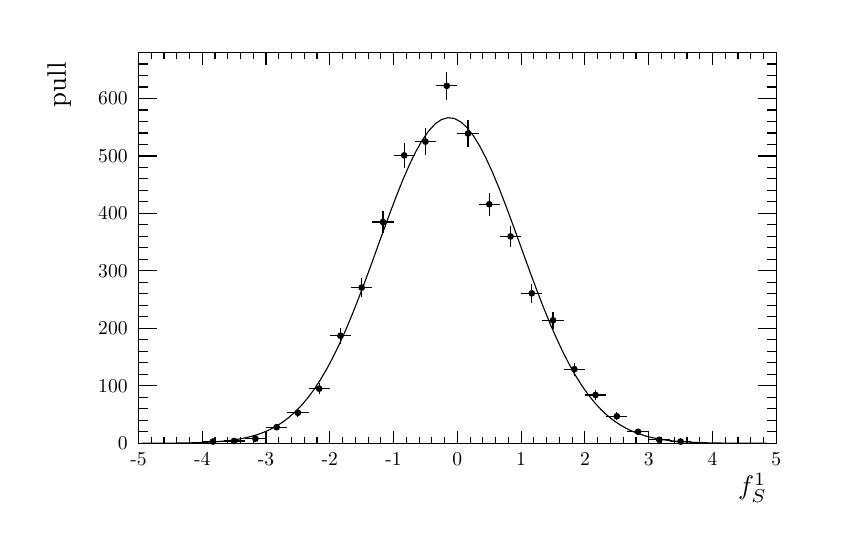
\begin{tikzpicture}
\pgfdeclareplotmark{cross} {
\pgfpathmoveto{\pgfpoint{-0.3\pgfplotmarksize}{\pgfplotmarksize}}
\pgfpathlineto{\pgfpoint{+0.3\pgfplotmarksize}{\pgfplotmarksize}}
\pgfpathlineto{\pgfpoint{+0.3\pgfplotmarksize}{0.3\pgfplotmarksize}}
\pgfpathlineto{\pgfpoint{+1\pgfplotmarksize}{0.3\pgfplotmarksize}}
\pgfpathlineto{\pgfpoint{+1\pgfplotmarksize}{-0.3\pgfplotmarksize}}
\pgfpathlineto{\pgfpoint{+0.3\pgfplotmarksize}{-0.3\pgfplotmarksize}}
\pgfpathlineto{\pgfpoint{+0.3\pgfplotmarksize}{-1.\pgfplotmarksize}}
\pgfpathlineto{\pgfpoint{-0.3\pgfplotmarksize}{-1.\pgfplotmarksize}}
\pgfpathlineto{\pgfpoint{-0.3\pgfplotmarksize}{-0.3\pgfplotmarksize}}
\pgfpathlineto{\pgfpoint{-1.\pgfplotmarksize}{-0.3\pgfplotmarksize}}
\pgfpathlineto{\pgfpoint{-1.\pgfplotmarksize}{0.3\pgfplotmarksize}}
\pgfpathlineto{\pgfpoint{-0.3\pgfplotmarksize}{0.3\pgfplotmarksize}}
\pgfpathclose
\pgfusepathqstroke
}
\pgfdeclareplotmark{cross*} {
\pgfpathmoveto{\pgfpoint{-0.3\pgfplotmarksize}{\pgfplotmarksize}}
\pgfpathlineto{\pgfpoint{+0.3\pgfplotmarksize}{\pgfplotmarksize}}
\pgfpathlineto{\pgfpoint{+0.3\pgfplotmarksize}{0.3\pgfplotmarksize}}
\pgfpathlineto{\pgfpoint{+1\pgfplotmarksize}{0.3\pgfplotmarksize}}
\pgfpathlineto{\pgfpoint{+1\pgfplotmarksize}{-0.3\pgfplotmarksize}}
\pgfpathlineto{\pgfpoint{+0.3\pgfplotmarksize}{-0.3\pgfplotmarksize}}
\pgfpathlineto{\pgfpoint{+0.3\pgfplotmarksize}{-1.\pgfplotmarksize}}
\pgfpathlineto{\pgfpoint{-0.3\pgfplotmarksize}{-1.\pgfplotmarksize}}
\pgfpathlineto{\pgfpoint{-0.3\pgfplotmarksize}{-0.3\pgfplotmarksize}}
\pgfpathlineto{\pgfpoint{-1.\pgfplotmarksize}{-0.3\pgfplotmarksize}}
\pgfpathlineto{\pgfpoint{-1.\pgfplotmarksize}{0.3\pgfplotmarksize}}
\pgfpathlineto{\pgfpoint{-0.3\pgfplotmarksize}{0.3\pgfplotmarksize}}
\pgfpathclose
\pgfusepathqfillstroke
}
\pgfdeclareplotmark{newstar} {
\pgfpathmoveto{\pgfqpoint{0pt}{\pgfplotmarksize}}
\pgfpathlineto{\pgfqpointpolar{44}{0.5\pgfplotmarksize}}
\pgfpathlineto{\pgfqpointpolar{18}{\pgfplotmarksize}}
\pgfpathlineto{\pgfqpointpolar{-20}{0.5\pgfplotmarksize}}
\pgfpathlineto{\pgfqpointpolar{-54}{\pgfplotmarksize}}
\pgfpathlineto{\pgfqpointpolar{-90}{0.5\pgfplotmarksize}}
\pgfpathlineto{\pgfqpointpolar{234}{\pgfplotmarksize}}
\pgfpathlineto{\pgfqpointpolar{198}{0.5\pgfplotmarksize}}
\pgfpathlineto{\pgfqpointpolar{162}{\pgfplotmarksize}}
\pgfpathlineto{\pgfqpointpolar{134}{0.5\pgfplotmarksize}}
\pgfpathclose
\pgfusepathqstroke
}
\pgfdeclareplotmark{newstar*} {
\pgfpathmoveto{\pgfqpoint{0pt}{\pgfplotmarksize}}
\pgfpathlineto{\pgfqpointpolar{44}{0.5\pgfplotmarksize}}
\pgfpathlineto{\pgfqpointpolar{18}{\pgfplotmarksize}}
\pgfpathlineto{\pgfqpointpolar{-20}{0.5\pgfplotmarksize}}
\pgfpathlineto{\pgfqpointpolar{-54}{\pgfplotmarksize}}
\pgfpathlineto{\pgfqpointpolar{-90}{0.5\pgfplotmarksize}}
\pgfpathlineto{\pgfqpointpolar{234}{\pgfplotmarksize}}
\pgfpathlineto{\pgfqpointpolar{198}{0.5\pgfplotmarksize}}
\pgfpathlineto{\pgfqpointpolar{162}{\pgfplotmarksize}}
\pgfpathlineto{\pgfqpointpolar{134}{0.5\pgfplotmarksize}}
\pgfpathclose
\pgfusepathqfillstroke
}
\definecolor{c}{rgb}{1,1,1};
\draw [color=c, fill=c] (0,0) rectangle (10,6.27517);
\draw [color=c, fill=c] (1.4,1.00403) rectangle (9.5,5.96141);
\definecolor{c}{rgb}{0,0,0};
\draw [c] (1.4,1.00403) -- (1.4,5.96141) -- (9.5,5.96141) -- (9.5,1.00403) -- (1.4,1.00403);
\draw [c] (2.345,1.01328) -- (2.345,1.02592);
\draw [c] (2.345,1.02592) -- (2.345,1.03856);
\draw [c] (2.21,1.02592) -- (2.345,1.02592);
\draw [c] (2.345,1.02592) -- (2.48,1.02592);
\foreach \P in {(2.345,1.02592)}{\draw[mark options={color=c,fill=c},mark size=2.402402pt,mark=*,mark size=1pt] plot coordinates {\P};}
\draw [c] (2.615,1.01862) -- (2.615,1.03322);
\draw [c] (2.615,1.03322) -- (2.615,1.04781);
\draw [c] (2.48,1.03322) -- (2.615,1.03322);
\draw [c] (2.615,1.03322) -- (2.75,1.03322);
\foreach \P in {(2.615,1.03322)}{\draw[mark options={color=c,fill=c},mark size=2.402402pt,mark=*,mark size=1pt] plot coordinates {\P};}
\draw [c] (2.885,1.04177) -- (2.885,1.06241);
\draw [c] (2.885,1.06241) -- (2.885,1.08305);
\draw [c] (2.75,1.06241) -- (2.885,1.06241);
\draw [c] (2.885,1.06241) -- (3.02,1.06241);
\foreach \P in {(2.885,1.06241)}{\draw[mark options={color=c,fill=c},mark size=2.402402pt,mark=*,mark size=1pt] plot coordinates {\P};}
\draw [c] (3.155,1.16975) -- (3.155,1.20837);
\draw [c] (3.155,1.20837) -- (3.155,1.24699);
\draw [c] (3.02,1.20837) -- (3.155,1.20837);
\draw [c] (3.155,1.20837) -- (3.29,1.20837);
\foreach \P in {(3.155,1.20837)}{\draw[mark options={color=c,fill=c},mark size=2.402402pt,mark=*,mark size=1pt] plot coordinates {\P};}
\draw [c] (3.425,1.33769) -- (3.425,1.39082);
\draw [c] (3.425,1.39082) -- (3.425,1.44395);
\draw [c] (3.29,1.39082) -- (3.425,1.39082);
\draw [c] (3.425,1.39082) -- (3.56,1.39082);
\foreach \P in {(3.425,1.39082)}{\draw[mark options={color=c,fill=c},mark size=2.402402pt,mark=*,mark size=1pt] plot coordinates {\P};}
\draw [c] (3.695,1.6262) -- (3.695,1.69733);
\draw [c] (3.695,1.69733) -- (3.695,1.76846);
\draw [c] (3.56,1.69733) -- (3.695,1.69733);
\draw [c] (3.695,1.69733) -- (3.83,1.69733);
\foreach \P in {(3.695,1.69733)}{\draw[mark options={color=c,fill=c},mark size=2.402402pt,mark=*,mark size=1pt] plot coordinates {\P};}
\draw [c] (3.965,2.26894) -- (3.965,2.36874);
\draw [c] (3.965,2.36874) -- (3.965,2.46854);
\draw [c] (3.83,2.36874) -- (3.965,2.36874);
\draw [c] (3.965,2.36874) -- (4.1,2.36874);
\foreach \P in {(3.965,2.36874)}{\draw[mark options={color=c,fill=c},mark size=2.402402pt,mark=*,mark size=1pt] plot coordinates {\P};}
\draw [c] (4.235,2.86162) -- (4.235,2.98176);
\draw [c] (4.235,2.98176) -- (4.235,3.1019);
\draw [c] (4.1,2.98176) -- (4.235,2.98176);
\draw [c] (4.235,2.98176) -- (4.37,2.98176);
\foreach \P in {(4.235,2.98176)}{\draw[mark options={color=c,fill=c},mark size=2.402402pt,mark=*,mark size=1pt] plot coordinates {\P};}
\draw [c] (4.505,3.67053) -- (4.505,3.81373);
\draw [c] (4.505,3.81373) -- (4.505,3.95692);
\draw [c] (4.37,3.81373) -- (4.505,3.81373);
\draw [c] (4.505,3.81373) -- (4.64,3.81373);
\foreach \P in {(4.505,3.81373)}{\draw[mark options={color=c,fill=c},mark size=2.402402pt,mark=*,mark size=1pt] plot coordinates {\P};}
\draw [c] (4.775,4.49694) -- (4.775,4.66029);
\draw [c] (4.775,4.66029) -- (4.775,4.82364);
\draw [c] (4.64,4.66029) -- (4.775,4.66029);
\draw [c] (4.775,4.66029) -- (4.91,4.66029);
\foreach \P in {(4.775,4.66029)}{\draw[mark options={color=c,fill=c},mark size=2.402402pt,mark=*,mark size=1pt] plot coordinates {\P};}
\draw [c] (5.045,4.66822) -- (5.045,4.83544);
\draw [c] (5.045,4.83544) -- (5.045,5.00265);
\draw [c] (4.91,4.83544) -- (5.045,4.83544);
\draw [c] (5.045,4.83544) -- (5.18,4.83544);
\foreach \P in {(5.045,4.83544)}{\draw[mark options={color=c,fill=c},mark size=2.402402pt,mark=*,mark size=1pt] plot coordinates {\P};}
\draw [c] (5.315,5.36132) -- (5.315,5.54333);
\draw [c] (5.315,5.54333) -- (5.315,5.72534);
\draw [c] (5.18,5.54333) -- (5.315,5.54333);
\draw [c] (5.315,5.54333) -- (5.45,5.54333);
\foreach \P in {(5.315,5.54333)}{\draw[mark options={color=c,fill=c},mark size=2.402402pt,mark=*,mark size=1pt] plot coordinates {\P};}
\draw [c] (5.585,4.76818) -- (5.585,4.93761);
\draw [c] (5.585,4.93761) -- (5.585,5.10704);
\draw [c] (5.45,4.93761) -- (5.585,4.93761);
\draw [c] (5.585,4.93761) -- (5.72,4.93761);
\foreach \P in {(5.585,4.93761)}{\draw[mark options={color=c,fill=c},mark size=2.402402pt,mark=*,mark size=1pt] plot coordinates {\P};}
\draw [c] (5.855,3.89111) -- (5.855,4.03996);
\draw [c] (5.855,4.03996) -- (5.855,4.18881);
\draw [c] (5.72,4.03996) -- (5.855,4.03996);
\draw [c] (5.855,4.03996) -- (5.99,4.03996);
\foreach \P in {(5.855,4.03996)}{\draw[mark options={color=c,fill=c},mark size=2.402402pt,mark=*,mark size=1pt] plot coordinates {\P};}
\draw [c] (6.125,3.49281) -- (6.125,3.63128);
\draw [c] (6.125,3.63128) -- (6.125,3.76975);
\draw [c] (5.99,3.63128) -- (6.125,3.63128);
\draw [c] (6.125,3.63128) -- (6.26,3.63128);
\foreach \P in {(6.125,3.63128)}{\draw[mark options={color=c,fill=c},mark size=2.402402pt,mark=*,mark size=1pt] plot coordinates {\P};}
\draw [c] (6.395,2.79088) -- (6.395,2.90878);
\draw [c] (6.395,2.90878) -- (6.395,3.02669);
\draw [c] (6.26,2.90878) -- (6.395,2.90878);
\draw [c] (6.395,2.90878) -- (6.53,2.90878);
\foreach \P in {(6.395,2.90878)}{\draw[mark options={color=c,fill=c},mark size=2.402402pt,mark=*,mark size=1pt] plot coordinates {\P};}
\draw [c] (6.665,2.45902) -- (6.665,2.56578);
\draw [c] (6.665,2.56578) -- (6.665,2.67254);
\draw [c] (6.53,2.56578) -- (6.665,2.56578);
\draw [c] (6.665,2.56578) -- (6.8,2.56578);
\foreach \P in {(6.665,2.56578)}{\draw[mark options={color=c,fill=c},mark size=2.402402pt,mark=*,mark size=1pt] plot coordinates {\P};}
\draw [c] (6.935,1.86257) -- (6.935,1.94546);
\draw [c] (6.935,1.94546) -- (6.935,2.02835);
\draw [c] (6.8,1.94546) -- (6.935,1.94546);
\draw [c] (6.935,1.94546) -- (7.07,1.94546);
\foreach \P in {(6.935,1.94546)}{\draw[mark options={color=c,fill=c},mark size=2.402402pt,mark=*,mark size=1pt] plot coordinates {\P};}
\draw [c] (7.205,1.55017) -- (7.205,1.61705);
\draw [c] (7.205,1.61705) -- (7.205,1.68394);
\draw [c] (7.07,1.61705) -- (7.205,1.61705);
\draw [c] (7.205,1.61705) -- (7.34,1.61705);
\foreach \P in {(7.205,1.61705)}{\draw[mark options={color=c,fill=c},mark size=2.402402pt,mark=*,mark size=1pt] plot coordinates {\P};}
\draw [c] (7.475,1.297) -- (7.475,1.34703);
\draw [c] (7.475,1.34703) -- (7.475,1.39706);
\draw [c] (7.34,1.34703) -- (7.475,1.34703);
\draw [c] (7.475,1.34703) -- (7.61,1.34703);
\foreach \P in {(7.475,1.34703)}{\draw[mark options={color=c,fill=c},mark size=2.402402pt,mark=*,mark size=1pt] plot coordinates {\P};}
\draw [c] (7.745,1.11735) -- (7.745,1.14999);
\draw [c] (7.745,1.14999) -- (7.745,1.18262);
\draw [c] (7.61,1.14999) -- (7.745,1.14999);
\draw [c] (7.745,1.14999) -- (7.88,1.14999);
\foreach \P in {(7.745,1.14999)}{\draw[mark options={color=c,fill=c},mark size=2.402402pt,mark=*,mark size=1pt] plot coordinates {\P};}
\draw [c] (8.015,1.02994) -- (8.015,1.04781);
\draw [c] (8.015,1.04781) -- (8.015,1.06569);
\draw [c] (7.88,1.04781) -- (8.015,1.04781);
\draw [c] (8.015,1.04781) -- (8.15,1.04781);
\foreach \P in {(8.015,1.04781)}{\draw[mark options={color=c,fill=c},mark size=2.402402pt,mark=*,mark size=1pt] plot coordinates {\P};}
\draw [c] (8.285,1.01328) -- (8.285,1.02592);
\draw [c] (8.285,1.02592) -- (8.285,1.03856);
\draw [c] (8.15,1.02592) -- (8.285,1.02592);
\draw [c] (8.285,1.02592) -- (8.42,1.02592);
\foreach \P in {(8.285,1.02592)}{\draw[mark options={color=c,fill=c},mark size=2.402402pt,mark=*,mark size=1pt] plot coordinates {\P};}
\draw [c,line width=0.4] (1.4405,1.00403) -- (1.5215,1.00457) -- (1.6025,1.00482) -- (1.6835,1.00517) -- (1.7645,1.00566) -- (1.8455,1.00635) -- (1.9265,1.0073) -- (2.0075,1.00859) -- (2.0885,1.01035) -- (2.1695,1.01273) -- (2.2505,1.01589) --
 (2.3315,1.02008) -- (2.4125,1.02557) -- (2.4935,1.03271) -- (2.5745,1.04191) -- (2.6555,1.05366) -- (2.7365,1.06854) -- (2.8175,1.08721) -- (2.8985,1.11043) -- (2.9795,1.13904) -- (3.0605,1.17398) -- (3.1415,1.21625) -- (3.2225,1.26693) --
 (3.3035,1.3271) -- (3.3845,1.39789) -- (3.4655,1.48035) -- (3.5465,1.57547) -- (3.6275,1.68413) -- (3.7085,1.80699) -- (3.7895,1.94447) -- (3.8705,2.09671) -- (3.9515,2.26346) -- (4.0325,2.44408) -- (4.1135,2.63746) -- (4.1945,2.84202) --
 (4.2755,3.05571) -- (4.3565,3.27596) -- (4.4375,3.49978) -- (4.5185,3.72378) -- (4.5995,3.94423) -- (4.6805,4.15718) -- (4.7615,4.35858) -- (4.8425,4.54437) -- (4.9235,4.71064) -- (5.0045,4.85375) -- (5.0855,4.97048) -- (5.1665,5.05814) --
 (5.2475,5.11467) -- (5.3285,5.13874) -- (5.4095,5.12976);
\draw [c,line width=0.4] (5.4095,5.12976) -- (5.4905,5.08796) -- (5.5715,5.01432) -- (5.6525,4.91059) -- (5.7335,4.77918) -- (5.8145,4.62308) -- (5.8955,4.44575) -- (5.9765,4.25099) -- (6.0575,4.04281) -- (6.1385,3.82529) -- (6.2195,3.60244) --
 (6.3005,3.37809) -- (6.3815,3.15581) -- (6.4625,2.93878) -- (6.5435,2.72976) -- (6.6245,2.53103) -- (6.7055,2.34441) -- (6.7865,2.17121) -- (6.8675,2.01228) -- (6.9485,1.86804) -- (7.0295,1.73853) -- (7.1105,1.62345) -- (7.1915,1.52223) --
 (7.2725,1.43409) -- (7.3535,1.3581) -- (7.4345,1.29321) -- (7.5155,1.23832) -- (7.5965,1.19234) -- (7.6775,1.15418) -- (7.7585,1.12279) -- (7.8395,1.09722) -- (7.9205,1.07656) -- (8.0015,1.06004) -- (8.0825,1.04693) -- (8.1635,1.03663) --
 (8.2445,1.02861) -- (8.3255,1.02241) -- (8.4065,1.01766) -- (8.4875,1.01406) -- (8.5685,1.01135) -- (8.6495,1.00933) -- (8.7305,1.00784) -- (8.8115,1.00674) -- (8.8925,1.00595) -- (8.9735,1.00537) -- (9.0545,1.00496) -- (9.1355,1.00467) --
 (9.2165,1.00403) -- (9.2975,1.00403) -- (9.3785,1.00403);
\draw [c,line width=0.4] (9.3785,1.00403) -- (9.4595,1.00403);
\draw [c,line width=0.4] (1.4,1.00403) -- (9.5,1.00403);
\draw [anchor= east] (9.5,0.441772) node[scale=0.96888, rotate=0]{$f_\text{S}^1$};
\draw [c,line width=0.4] (1.4,1.15651) -- (1.4,1.00403);
\draw [c,line width=0.4] (1.562,1.08027) -- (1.562,1.00403);
\draw [c,line width=0.4] (1.724,1.08027) -- (1.724,1.00403);
\draw [c,line width=0.4] (1.886,1.08027) -- (1.886,1.00403);
\draw [c,line width=0.4] (2.048,1.08027) -- (2.048,1.00403);
\draw [c,line width=0.4] (2.21,1.15651) -- (2.21,1.00403);
\draw [c,line width=0.4] (2.372,1.08027) -- (2.372,1.00403);
\draw [c,line width=0.4] (2.534,1.08027) -- (2.534,1.00403);
\draw [c,line width=0.4] (2.696,1.08027) -- (2.696,1.00403);
\draw [c,line width=0.4] (2.858,1.08027) -- (2.858,1.00403);
\draw [c,line width=0.4] (3.02,1.15651) -- (3.02,1.00403);
\draw [c,line width=0.4] (3.182,1.08027) -- (3.182,1.00403);
\draw [c,line width=0.4] (3.344,1.08027) -- (3.344,1.00403);
\draw [c,line width=0.4] (3.506,1.08027) -- (3.506,1.00403);
\draw [c,line width=0.4] (3.668,1.08027) -- (3.668,1.00403);
\draw [c,line width=0.4] (3.83,1.15651) -- (3.83,1.00403);
\draw [c,line width=0.4] (3.992,1.08027) -- (3.992,1.00403);
\draw [c,line width=0.4] (4.154,1.08027) -- (4.154,1.00403);
\draw [c,line width=0.4] (4.316,1.08027) -- (4.316,1.00403);
\draw [c,line width=0.4] (4.478,1.08027) -- (4.478,1.00403);
\draw [c,line width=0.4] (4.64,1.15651) -- (4.64,1.00403);
\draw [c,line width=0.4] (4.802,1.08027) -- (4.802,1.00403);
\draw [c,line width=0.4] (4.964,1.08027) -- (4.964,1.00403);
\draw [c,line width=0.4] (5.126,1.08027) -- (5.126,1.00403);
\draw [c,line width=0.4] (5.288,1.08027) -- (5.288,1.00403);
\draw [c,line width=0.4] (5.45,1.15651) -- (5.45,1.00403);
\draw [c,line width=0.4] (5.612,1.08027) -- (5.612,1.00403);
\draw [c,line width=0.4] (5.774,1.08027) -- (5.774,1.00403);
\draw [c,line width=0.4] (5.936,1.08027) -- (5.936,1.00403);
\draw [c,line width=0.4] (6.098,1.08027) -- (6.098,1.00403);
\draw [c,line width=0.4] (6.26,1.15651) -- (6.26,1.00403);
\draw [c,line width=0.4] (6.422,1.08027) -- (6.422,1.00403);
\draw [c,line width=0.4] (6.584,1.08027) -- (6.584,1.00403);
\draw [c,line width=0.4] (6.746,1.08027) -- (6.746,1.00403);
\draw [c,line width=0.4] (6.908,1.08027) -- (6.908,1.00403);
\draw [c,line width=0.4] (7.07,1.15651) -- (7.07,1.00403);
\draw [c,line width=0.4] (7.232,1.08027) -- (7.232,1.00403);
\draw [c,line width=0.4] (7.394,1.08027) -- (7.394,1.00403);
\draw [c,line width=0.4] (7.556,1.08027) -- (7.556,1.00403);
\draw [c,line width=0.4] (7.718,1.08027) -- (7.718,1.00403);
\draw [c,line width=0.4] (7.88,1.15651) -- (7.88,1.00403);
\draw [c,line width=0.4] (8.042,1.08027) -- (8.042,1.00403);
\draw [c,line width=0.4] (8.204,1.08027) -- (8.204,1.00403);
\draw [c,line width=0.4] (8.366,1.08027) -- (8.366,1.00403);
\draw [c,line width=0.4] (8.528,1.08027) -- (8.528,1.00403);
\draw [c,line width=0.4] (8.69,1.15651) -- (8.69,1.00403);
\draw [c,line width=0.4] (8.852,1.08027) -- (8.852,1.00403);
\draw [c,line width=0.4] (9.014,1.08027) -- (9.014,1.00403);
\draw [c,line width=0.4] (9.176,1.08027) -- (9.176,1.00403);
\draw [c,line width=0.4] (9.338,1.08027) -- (9.338,1.00403);
\draw [c,line width=0.4] (9.5,1.15651) -- (9.5,1.00403);
\draw [anchor=base] (1.4,0.721644) node[scale=0.708027, rotate=0]{-5};
\draw [anchor=base] (2.21,0.721644) node[scale=0.708027, rotate=0]{-4};
\draw [anchor=base] (3.02,0.721644) node[scale=0.708027, rotate=0]{-3};
\draw [anchor=base] (3.83,0.721644) node[scale=0.708027, rotate=0]{-2};
\draw [anchor=base] (4.64,0.721644) node[scale=0.708027, rotate=0]{-1};
\draw [anchor=base] (5.45,0.721644) node[scale=0.708027, rotate=0]{0};
\draw [anchor=base] (6.26,0.721644) node[scale=0.708027, rotate=0]{1};
\draw [anchor=base] (7.07,0.721644) node[scale=0.708027, rotate=0]{2};
\draw [anchor=base] (7.88,0.721644) node[scale=0.708027, rotate=0]{3};
\draw [anchor=base] (8.69,0.721644) node[scale=0.708027, rotate=0]{4};
\draw [anchor=base] (9.5,0.721644) node[scale=0.708027, rotate=0]{5};
\draw [c,line width=0.4] (1.4,5.96141) -- (9.5,5.96141);
\draw [c,line width=0.4] (1.4,5.80892) -- (1.4,5.96141);
\draw [c,line width=0.4] (1.562,5.88517) -- (1.562,5.96141);
\draw [c,line width=0.4] (1.724,5.88517) -- (1.724,5.96141);
\draw [c,line width=0.4] (1.886,5.88517) -- (1.886,5.96141);
\draw [c,line width=0.4] (2.048,5.88517) -- (2.048,5.96141);
\draw [c,line width=0.4] (2.21,5.80892) -- (2.21,5.96141);
\draw [c,line width=0.4] (2.372,5.88517) -- (2.372,5.96141);
\draw [c,line width=0.4] (2.534,5.88517) -- (2.534,5.96141);
\draw [c,line width=0.4] (2.696,5.88517) -- (2.696,5.96141);
\draw [c,line width=0.4] (2.858,5.88517) -- (2.858,5.96141);
\draw [c,line width=0.4] (3.02,5.80892) -- (3.02,5.96141);
\draw [c,line width=0.4] (3.182,5.88517) -- (3.182,5.96141);
\draw [c,line width=0.4] (3.344,5.88517) -- (3.344,5.96141);
\draw [c,line width=0.4] (3.506,5.88517) -- (3.506,5.96141);
\draw [c,line width=0.4] (3.668,5.88517) -- (3.668,5.96141);
\draw [c,line width=0.4] (3.83,5.80892) -- (3.83,5.96141);
\draw [c,line width=0.4] (3.992,5.88517) -- (3.992,5.96141);
\draw [c,line width=0.4] (4.154,5.88517) -- (4.154,5.96141);
\draw [c,line width=0.4] (4.316,5.88517) -- (4.316,5.96141);
\draw [c,line width=0.4] (4.478,5.88517) -- (4.478,5.96141);
\draw [c,line width=0.4] (4.64,5.80892) -- (4.64,5.96141);
\draw [c,line width=0.4] (4.802,5.88517) -- (4.802,5.96141);
\draw [c,line width=0.4] (4.964,5.88517) -- (4.964,5.96141);
\draw [c,line width=0.4] (5.126,5.88517) -- (5.126,5.96141);
\draw [c,line width=0.4] (5.288,5.88517) -- (5.288,5.96141);
\draw [c,line width=0.4] (5.45,5.80892) -- (5.45,5.96141);
\draw [c,line width=0.4] (5.612,5.88517) -- (5.612,5.96141);
\draw [c,line width=0.4] (5.774,5.88517) -- (5.774,5.96141);
\draw [c,line width=0.4] (5.936,5.88517) -- (5.936,5.96141);
\draw [c,line width=0.4] (6.098,5.88517) -- (6.098,5.96141);
\draw [c,line width=0.4] (6.26,5.80892) -- (6.26,5.96141);
\draw [c,line width=0.4] (6.422,5.88517) -- (6.422,5.96141);
\draw [c,line width=0.4] (6.584,5.88517) -- (6.584,5.96141);
\draw [c,line width=0.4] (6.746,5.88517) -- (6.746,5.96141);
\draw [c,line width=0.4] (6.908,5.88517) -- (6.908,5.96141);
\draw [c,line width=0.4] (7.07,5.80892) -- (7.07,5.96141);
\draw [c,line width=0.4] (7.232,5.88517) -- (7.232,5.96141);
\draw [c,line width=0.4] (7.394,5.88517) -- (7.394,5.96141);
\draw [c,line width=0.4] (7.556,5.88517) -- (7.556,5.96141);
\draw [c,line width=0.4] (7.718,5.88517) -- (7.718,5.96141);
\draw [c,line width=0.4] (7.88,5.80892) -- (7.88,5.96141);
\draw [c,line width=0.4] (8.042,5.88517) -- (8.042,5.96141);
\draw [c,line width=0.4] (8.204,5.88517) -- (8.204,5.96141);
\draw [c,line width=0.4] (8.366,5.88517) -- (8.366,5.96141);
\draw [c,line width=0.4] (8.528,5.88517) -- (8.528,5.96141);
\draw [c,line width=0.4] (8.69,5.80892) -- (8.69,5.96141);
\draw [c,line width=0.4] (8.852,5.88517) -- (8.852,5.96141);
\draw [c,line width=0.4] (9.014,5.88517) -- (9.014,5.96141);
\draw [c,line width=0.4] (9.176,5.88517) -- (9.176,5.96141);
\draw [c,line width=0.4] (9.338,5.88517) -- (9.338,5.96141);
\draw [c,line width=0.4] (9.5,5.80892) -- (9.5,5.96141);
\draw [c,line width=0.4] (1.4,1.00403) -- (1.4,5.96141);
\draw [anchor= east] (0.392,5.96141) node[scale=0.96888, rotate=90]{pull};
\draw [c,line width=0.4] (1.637,1.00403) -- (1.4,1.00403);
\draw [c,line width=0.4] (1.5185,1.14999) -- (1.4,1.14999);
\draw [c,line width=0.4] (1.5185,1.29594) -- (1.4,1.29594);
\draw [c,line width=0.4] (1.5185,1.4419) -- (1.4,1.4419);
\draw [c,line width=0.4] (1.5185,1.58786) -- (1.4,1.58786);
\draw [c,line width=0.4] (1.637,1.73382) -- (1.4,1.73382);
\draw [c,line width=0.4] (1.5185,1.87978) -- (1.4,1.87978);
\draw [c,line width=0.4] (1.5185,2.02574) -- (1.4,2.02574);
\draw [c,line width=0.4] (1.5185,2.17169) -- (1.4,2.17169);
\draw [c,line width=0.4] (1.5185,2.31765) -- (1.4,2.31765);
\draw [c,line width=0.4] (1.637,2.46361) -- (1.4,2.46361);
\draw [c,line width=0.4] (1.5185,2.60957) -- (1.4,2.60957);
\draw [c,line width=0.4] (1.5185,2.75553) -- (1.4,2.75553);
\draw [c,line width=0.4] (1.5185,2.90149) -- (1.4,2.90149);
\draw [c,line width=0.4] (1.5185,3.04744) -- (1.4,3.04744);
\draw [c,line width=0.4] (1.637,3.1934) -- (1.4,3.1934);
\draw [c,line width=0.4] (1.5185,3.33936) -- (1.4,3.33936);
\draw [c,line width=0.4] (1.5185,3.48532) -- (1.4,3.48532);
\draw [c,line width=0.4] (1.5185,3.63128) -- (1.4,3.63128);
\draw [c,line width=0.4] (1.5185,3.77724) -- (1.4,3.77724);
\draw [c,line width=0.4] (1.637,3.9232) -- (1.4,3.9232);
\draw [c,line width=0.4] (1.5185,4.06915) -- (1.4,4.06915);
\draw [c,line width=0.4] (1.5185,4.21511) -- (1.4,4.21511);
\draw [c,line width=0.4] (1.5185,4.36107) -- (1.4,4.36107);
\draw [c,line width=0.4] (1.5185,4.50703) -- (1.4,4.50703);
\draw [c,line width=0.4] (1.637,4.65299) -- (1.4,4.65299);
\draw [c,line width=0.4] (1.5185,4.79895) -- (1.4,4.79895);
\draw [c,line width=0.4] (1.5185,4.9449) -- (1.4,4.9449);
\draw [c,line width=0.4] (1.5185,5.09086) -- (1.4,5.09086);
\draw [c,line width=0.4] (1.5185,5.23682) -- (1.4,5.23682);
\draw [c,line width=0.4] (1.637,5.38278) -- (1.4,5.38278);
\draw [c,line width=0.4] (1.637,5.38278) -- (1.4,5.38278);
\draw [c,line width=0.4] (1.5185,5.52874) -- (1.4,5.52874);
\draw [c,line width=0.4] (1.5185,5.6747) -- (1.4,5.6747);
\draw [c,line width=0.4] (1.5185,5.82065) -- (1.4,5.82065);
\draw [anchor= east] (1.35,1.00403) node[scale=0.708027, rotate=0]{0};
\draw [anchor= east] (1.35,1.73382) node[scale=0.708027, rotate=0]{100};
\draw [anchor= east] (1.35,2.46361) node[scale=0.708027, rotate=0]{200};
\draw [anchor= east] (1.35,3.1934) node[scale=0.708027, rotate=0]{300};
\draw [anchor= east] (1.35,3.9232) node[scale=0.708027, rotate=0]{400};
\draw [anchor= east] (1.35,4.65299) node[scale=0.708027, rotate=0]{500};
\draw [anchor= east] (1.35,5.38278) node[scale=0.708027, rotate=0]{600};
\draw [c,line width=0.4] (9.5,1.00403) -- (9.5,5.96141);
\draw [c,line width=0.4] (9.263,1.00403) -- (9.5,1.00403);
\draw [c,line width=0.4] (9.3815,1.14999) -- (9.5,1.14999);
\draw [c,line width=0.4] (9.3815,1.29594) -- (9.5,1.29594);
\draw [c,line width=0.4] (9.3815,1.4419) -- (9.5,1.4419);
\draw [c,line width=0.4] (9.3815,1.58786) -- (9.5,1.58786);
\draw [c,line width=0.4] (9.263,1.73382) -- (9.5,1.73382);
\draw [c,line width=0.4] (9.3815,1.87978) -- (9.5,1.87978);
\draw [c,line width=0.4] (9.3815,2.02574) -- (9.5,2.02574);
\draw [c,line width=0.4] (9.3815,2.17169) -- (9.5,2.17169);
\draw [c,line width=0.4] (9.3815,2.31765) -- (9.5,2.31765);
\draw [c,line width=0.4] (9.263,2.46361) -- (9.5,2.46361);
\draw [c,line width=0.4] (9.3815,2.60957) -- (9.5,2.60957);
\draw [c,line width=0.4] (9.3815,2.75553) -- (9.5,2.75553);
\draw [c,line width=0.4] (9.3815,2.90149) -- (9.5,2.90149);
\draw [c,line width=0.4] (9.3815,3.04744) -- (9.5,3.04744);
\draw [c,line width=0.4] (9.263,3.1934) -- (9.5,3.1934);
\draw [c,line width=0.4] (9.3815,3.33936) -- (9.5,3.33936);
\draw [c,line width=0.4] (9.3815,3.48532) -- (9.5,3.48532);
\draw [c,line width=0.4] (9.3815,3.63128) -- (9.5,3.63128);
\draw [c,line width=0.4] (9.3815,3.77724) -- (9.5,3.77724);
\draw [c,line width=0.4] (9.263,3.9232) -- (9.5,3.9232);
\draw [c,line width=0.4] (9.3815,4.06915) -- (9.5,4.06915);
\draw [c,line width=0.4] (9.3815,4.21511) -- (9.5,4.21511);
\draw [c,line width=0.4] (9.3815,4.36107) -- (9.5,4.36107);
\draw [c,line width=0.4] (9.3815,4.50703) -- (9.5,4.50703);
\draw [c,line width=0.4] (9.263,4.65299) -- (9.5,4.65299);
\draw [c,line width=0.4] (9.3815,4.79895) -- (9.5,4.79895);
\draw [c,line width=0.4] (9.3815,4.9449) -- (9.5,4.9449);
\draw [c,line width=0.4] (9.3815,5.09086) -- (9.5,5.09086);
\draw [c,line width=0.4] (9.3815,5.23682) -- (9.5,5.23682);
\draw [c,line width=0.4] (9.263,5.38278) -- (9.5,5.38278);
\draw [c,line width=0.4] (9.263,5.38278) -- (9.5,5.38278);
\draw [c,line width=0.4] (9.3815,5.52874) -- (9.5,5.52874);
\draw [c,line width=0.4] (9.3815,5.6747) -- (9.5,5.6747);
\draw [c,line width=0.4] (9.3815,5.82065) -- (9.5,5.82065);
\end{tikzpicture}
}
    \caption{}
    \label{pull_ASMag2_bin1}
  \end{subfigure}%
  \hfill%
  \begin{subfigure}{0.5\textwidth}
    \tikzsetnextfilename{pull_ASPhase_bin1}
    \scalebox{0.60}{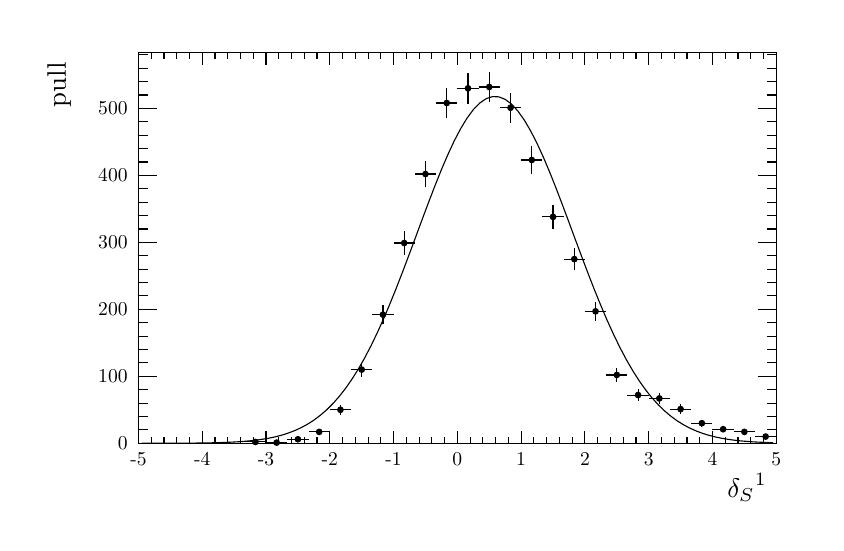
\begin{tikzpicture}
\pgfdeclareplotmark{cross} {
\pgfpathmoveto{\pgfpoint{-0.3\pgfplotmarksize}{\pgfplotmarksize}}
\pgfpathlineto{\pgfpoint{+0.3\pgfplotmarksize}{\pgfplotmarksize}}
\pgfpathlineto{\pgfpoint{+0.3\pgfplotmarksize}{0.3\pgfplotmarksize}}
\pgfpathlineto{\pgfpoint{+1\pgfplotmarksize}{0.3\pgfplotmarksize}}
\pgfpathlineto{\pgfpoint{+1\pgfplotmarksize}{-0.3\pgfplotmarksize}}
\pgfpathlineto{\pgfpoint{+0.3\pgfplotmarksize}{-0.3\pgfplotmarksize}}
\pgfpathlineto{\pgfpoint{+0.3\pgfplotmarksize}{-1.\pgfplotmarksize}}
\pgfpathlineto{\pgfpoint{-0.3\pgfplotmarksize}{-1.\pgfplotmarksize}}
\pgfpathlineto{\pgfpoint{-0.3\pgfplotmarksize}{-0.3\pgfplotmarksize}}
\pgfpathlineto{\pgfpoint{-1.\pgfplotmarksize}{-0.3\pgfplotmarksize}}
\pgfpathlineto{\pgfpoint{-1.\pgfplotmarksize}{0.3\pgfplotmarksize}}
\pgfpathlineto{\pgfpoint{-0.3\pgfplotmarksize}{0.3\pgfplotmarksize}}
\pgfpathclose
\pgfusepathqstroke
}
\pgfdeclareplotmark{cross*} {
\pgfpathmoveto{\pgfpoint{-0.3\pgfplotmarksize}{\pgfplotmarksize}}
\pgfpathlineto{\pgfpoint{+0.3\pgfplotmarksize}{\pgfplotmarksize}}
\pgfpathlineto{\pgfpoint{+0.3\pgfplotmarksize}{0.3\pgfplotmarksize}}
\pgfpathlineto{\pgfpoint{+1\pgfplotmarksize}{0.3\pgfplotmarksize}}
\pgfpathlineto{\pgfpoint{+1\pgfplotmarksize}{-0.3\pgfplotmarksize}}
\pgfpathlineto{\pgfpoint{+0.3\pgfplotmarksize}{-0.3\pgfplotmarksize}}
\pgfpathlineto{\pgfpoint{+0.3\pgfplotmarksize}{-1.\pgfplotmarksize}}
\pgfpathlineto{\pgfpoint{-0.3\pgfplotmarksize}{-1.\pgfplotmarksize}}
\pgfpathlineto{\pgfpoint{-0.3\pgfplotmarksize}{-0.3\pgfplotmarksize}}
\pgfpathlineto{\pgfpoint{-1.\pgfplotmarksize}{-0.3\pgfplotmarksize}}
\pgfpathlineto{\pgfpoint{-1.\pgfplotmarksize}{0.3\pgfplotmarksize}}
\pgfpathlineto{\pgfpoint{-0.3\pgfplotmarksize}{0.3\pgfplotmarksize}}
\pgfpathclose
\pgfusepathqfillstroke
}
\pgfdeclareplotmark{newstar} {
\pgfpathmoveto{\pgfqpoint{0pt}{\pgfplotmarksize}}
\pgfpathlineto{\pgfqpointpolar{44}{0.5\pgfplotmarksize}}
\pgfpathlineto{\pgfqpointpolar{18}{\pgfplotmarksize}}
\pgfpathlineto{\pgfqpointpolar{-20}{0.5\pgfplotmarksize}}
\pgfpathlineto{\pgfqpointpolar{-54}{\pgfplotmarksize}}
\pgfpathlineto{\pgfqpointpolar{-90}{0.5\pgfplotmarksize}}
\pgfpathlineto{\pgfqpointpolar{234}{\pgfplotmarksize}}
\pgfpathlineto{\pgfqpointpolar{198}{0.5\pgfplotmarksize}}
\pgfpathlineto{\pgfqpointpolar{162}{\pgfplotmarksize}}
\pgfpathlineto{\pgfqpointpolar{134}{0.5\pgfplotmarksize}}
\pgfpathclose
\pgfusepathqstroke
}
\pgfdeclareplotmark{newstar*} {
\pgfpathmoveto{\pgfqpoint{0pt}{\pgfplotmarksize}}
\pgfpathlineto{\pgfqpointpolar{44}{0.5\pgfplotmarksize}}
\pgfpathlineto{\pgfqpointpolar{18}{\pgfplotmarksize}}
\pgfpathlineto{\pgfqpointpolar{-20}{0.5\pgfplotmarksize}}
\pgfpathlineto{\pgfqpointpolar{-54}{\pgfplotmarksize}}
\pgfpathlineto{\pgfqpointpolar{-90}{0.5\pgfplotmarksize}}
\pgfpathlineto{\pgfqpointpolar{234}{\pgfplotmarksize}}
\pgfpathlineto{\pgfqpointpolar{198}{0.5\pgfplotmarksize}}
\pgfpathlineto{\pgfqpointpolar{162}{\pgfplotmarksize}}
\pgfpathlineto{\pgfqpointpolar{134}{0.5\pgfplotmarksize}}
\pgfpathclose
\pgfusepathqfillstroke
}
\definecolor{c}{rgb}{1,1,1};
\draw [color=c, fill=c] (0,0) rectangle (10,6.27517);
\draw [color=c, fill=c] (1.4,1.00403) rectangle (9.5,5.96141);
\definecolor{c}{rgb}{0,0,0};
\draw [c] (1.4,1.00403) -- (1.4,5.96141) -- (9.5,5.96141) -- (9.5,1.00403) -- (1.4,1.00403);
\draw [c] (2.885,1.00901) -- (2.885,1.02104);
\draw [c] (2.885,1.02104) -- (2.885,1.03307);
\draw [c] (2.75,1.02104) -- (2.885,1.02104);
\draw [c] (2.885,1.02104) -- (3.02,1.02104);
\foreach \P in {(2.885,1.02104)}{\draw[mark options={color=c,fill=c},mark size=2.402402pt,mark=*,mark size=1pt] plot coordinates {\P};}
\draw [c] (3.155,1.00403) -- (3.155,1.01253);
\draw [c] (3.155,1.01253) -- (3.155,1.02104);
\draw [c] (3.02,1.01253) -- (3.155,1.01253);
\draw [c] (3.155,1.01253) -- (3.29,1.01253);
\foreach \P in {(3.155,1.01253)}{\draw[mark options={color=c,fill=c},mark size=2.402402pt,mark=*,mark size=1pt] plot coordinates {\P};}
\draw [c] (3.425,1.03423) -- (3.425,1.05506);
\draw [c] (3.425,1.05506) -- (3.425,1.0759);
\draw [c] (3.29,1.05506) -- (3.425,1.05506);
\draw [c] (3.425,1.05506) -- (3.56,1.05506);
\foreach \P in {(3.425,1.05506)}{\draw[mark options={color=c,fill=c},mark size=2.402402pt,mark=*,mark size=1pt] plot coordinates {\P};}
\draw [c] (3.695,1.11356) -- (3.695,1.14863);
\draw [c] (3.695,1.14863) -- (3.695,1.1837);
\draw [c] (3.56,1.14863) -- (3.695,1.14863);
\draw [c] (3.695,1.14863) -- (3.83,1.14863);
\foreach \P in {(3.695,1.14863)}{\draw[mark options={color=c,fill=c},mark size=2.402402pt,mark=*,mark size=1pt] plot coordinates {\P};}
\draw [c] (3.965,1.36918) -- (3.965,1.42932);
\draw [c] (3.965,1.42932) -- (3.965,1.48947);
\draw [c] (3.83,1.42932) -- (3.965,1.42932);
\draw [c] (3.965,1.42932) -- (4.1,1.42932);
\foreach \P in {(3.965,1.42932)}{\draw[mark options={color=c,fill=c},mark size=2.402402pt,mark=*,mark size=1pt] plot coordinates {\P};}
\draw [c] (4.235,1.85046) -- (4.235,1.93967);
\draw [c] (4.235,1.93967) -- (4.235,2.02888);
\draw [c] (4.1,1.93967) -- (4.235,1.93967);
\draw [c] (4.235,1.93967) -- (4.37,1.93967);
\foreach \P in {(4.235,1.93967)}{\draw[mark options={color=c,fill=c},mark size=2.402402pt,mark=*,mark size=1pt] plot coordinates {\P};}
\draw [c] (4.505,2.51929) -- (4.505,2.63716);
\draw [c] (4.505,2.63716) -- (4.505,2.75502);
\draw [c] (4.37,2.63716) -- (4.505,2.63716);
\draw [c] (4.505,2.63716) -- (4.64,2.63716);
\foreach \P in {(4.505,2.63716)}{\draw[mark options={color=c,fill=c},mark size=2.402402pt,mark=*,mark size=1pt] plot coordinates {\P};}
\draw [c] (4.775,3.4002) -- (4.775,3.54728);
\draw [c] (4.775,3.54728) -- (4.775,3.69437);
\draw [c] (4.64,3.54728) -- (4.775,3.54728);
\draw [c] (4.775,3.54728) -- (4.91,3.54728);
\foreach \P in {(4.775,3.54728)}{\draw[mark options={color=c,fill=c},mark size=2.402402pt,mark=*,mark size=1pt] plot coordinates {\P};}
\draw [c] (5.045,4.25285) -- (5.045,4.42339);
\draw [c] (5.045,4.42339) -- (5.045,4.59393);
\draw [c] (4.91,4.42339) -- (5.045,4.42339);
\draw [c] (5.045,4.42339) -- (5.18,4.42339);
\foreach \P in {(5.045,4.42339)}{\draw[mark options={color=c,fill=c},mark size=2.402402pt,mark=*,mark size=1pt] plot coordinates {\P};}
\draw [c] (5.315,5.1333) -- (5.315,5.32501);
\draw [c] (5.315,5.32501) -- (5.315,5.51673);
\draw [c] (5.18,5.32501) -- (5.315,5.32501);
\draw [c] (5.315,5.32501) -- (5.45,5.32501);
\foreach \P in {(5.315,5.32501)}{\draw[mark options={color=c,fill=c},mark size=2.402402pt,mark=*,mark size=1pt] plot coordinates {\P};}
\draw [c] (5.585,5.31632) -- (5.585,5.51214);
\draw [c] (5.585,5.51214) -- (5.585,5.70796);
\draw [c] (5.45,5.51214) -- (5.585,5.51214);
\draw [c] (5.585,5.51214) -- (5.72,5.51214);
\foreach \P in {(5.585,5.51214)}{\draw[mark options={color=c,fill=c},mark size=2.402402pt,mark=*,mark size=1pt] plot coordinates {\P};}
\draw [c] (5.855,5.33297) -- (5.855,5.52915);
\draw [c] (5.855,5.52915) -- (5.855,5.72534);
\draw [c] (5.72,5.52915) -- (5.855,5.52915);
\draw [c] (5.855,5.52915) -- (5.99,5.52915);
\foreach \P in {(5.855,5.52915)}{\draw[mark options={color=c,fill=c},mark size=2.402402pt,mark=*,mark size=1pt] plot coordinates {\P};}
\draw [c] (6.125,5.07509) -- (6.125,5.26547);
\draw [c] (6.125,5.26547) -- (6.125,5.45586);
\draw [c] (5.99,5.26547) -- (6.125,5.26547);
\draw [c] (6.125,5.26547) -- (6.26,5.26547);
\foreach \P in {(6.125,5.26547)}{\draw[mark options={color=c,fill=c},mark size=2.402402pt,mark=*,mark size=1pt] plot coordinates {\P};}
\draw [c] (6.395,4.42707) -- (6.395,4.60201);
\draw [c] (6.395,4.60201) -- (6.395,4.77695);
\draw [c] (6.26,4.60201) -- (6.395,4.60201);
\draw [c] (6.395,4.60201) -- (6.53,4.60201);
\foreach \P in {(6.395,4.60201)}{\draw[mark options={color=c,fill=c},mark size=2.402402pt,mark=*,mark size=1pt] plot coordinates {\P};}
\draw [c] (6.665,3.72264) -- (6.665,3.87901);
\draw [c] (6.665,3.87901) -- (6.665,4.03539);
\draw [c] (6.53,3.87901) -- (6.665,3.87901);
\draw [c] (6.665,3.87901) -- (6.8,3.87901);
\foreach \P in {(6.665,3.87901)}{\draw[mark options={color=c,fill=c},mark size=2.402402pt,mark=*,mark size=1pt] plot coordinates {\P};}
\draw [c] (6.935,3.20209) -- (6.935,3.34314);
\draw [c] (6.935,3.34314) -- (6.935,3.4842);
\draw [c] (6.8,3.34314) -- (6.935,3.34314);
\draw [c] (6.935,3.34314) -- (7.07,3.34314);
\foreach \P in {(6.935,3.34314)}{\draw[mark options={color=c,fill=c},mark size=2.402402pt,mark=*,mark size=1pt] plot coordinates {\P};}
\draw [c] (7.205,2.5603) -- (7.205,2.67969);
\draw [c] (7.205,2.67969) -- (7.205,2.79907);
\draw [c] (7.07,2.67969) -- (7.205,2.67969);
\draw [c] (7.205,2.67969) -- (7.34,2.67969);
\foreach \P in {(7.205,2.67969)}{\draw[mark options={color=c,fill=c},mark size=2.402402pt,mark=*,mark size=1pt] plot coordinates {\P};}
\draw [c] (7.475,1.78572) -- (7.475,1.87163);
\draw [c] (7.475,1.87163) -- (7.475,1.95753);
\draw [c] (7.34,1.87163) -- (7.475,1.87163);
\draw [c] (7.475,1.87163) -- (7.61,1.87163);
\foreach \P in {(7.475,1.87163)}{\draw[mark options={color=c,fill=c},mark size=2.402402pt,mark=*,mark size=1pt] plot coordinates {\P};}
\draw [c] (7.745,1.54428) -- (7.745,1.61645);
\draw [c] (7.745,1.61645) -- (7.745,1.68862);
\draw [c] (7.61,1.61645) -- (7.745,1.61645);
\draw [c] (7.745,1.61645) -- (7.88,1.61645);
\foreach \P in {(7.745,1.61645)}{\draw[mark options={color=c,fill=c},mark size=2.402402pt,mark=*,mark size=1pt] plot coordinates {\P};}
\draw [c] (8.015,1.5043) -- (8.015,1.57392);
\draw [c] (8.015,1.57392) -- (8.015,1.64354);
\draw [c] (7.88,1.57392) -- (8.015,1.57392);
\draw [c] (8.015,1.57392) -- (8.15,1.57392);
\foreach \P in {(8.015,1.57392)}{\draw[mark options={color=c,fill=c},mark size=2.402402pt,mark=*,mark size=1pt] plot coordinates {\P};}
\draw [c] (8.285,1.37708) -- (8.285,1.43783);
\draw [c] (8.285,1.43783) -- (8.285,1.49857);
\draw [c] (8.15,1.43783) -- (8.285,1.43783);
\draw [c] (8.285,1.43783) -- (8.42,1.43783);
\foreach \P in {(8.285,1.43783)}{\draw[mark options={color=c,fill=c},mark size=2.402402pt,mark=*,mark size=1pt] plot coordinates {\P};}
\draw [c] (8.555,1.21261) -- (8.555,1.2592);
\draw [c] (8.555,1.2592) -- (8.555,1.30579);
\draw [c] (8.42,1.2592) -- (8.555,1.2592);
\draw [c] (8.555,1.2592) -- (8.69,1.2592);
\foreach \P in {(8.555,1.2592)}{\draw[mark options={color=c,fill=c},mark size=2.402402pt,mark=*,mark size=1pt] plot coordinates {\P};}
\draw [c] (8.825,1.14367) -- (8.825,1.18265);
\draw [c] (8.825,1.18265) -- (8.825,1.22163);
\draw [c] (8.69,1.18265) -- (8.825,1.18265);
\draw [c] (8.825,1.18265) -- (8.96,1.18265);
\foreach \P in {(8.825,1.18265)}{\draw[mark options={color=c,fill=c},mark size=2.402402pt,mark=*,mark size=1pt] plot coordinates {\P};}
\draw [c] (9.095,1.11356) -- (9.095,1.14863);
\draw [c] (9.095,1.14863) -- (9.095,1.1837);
\draw [c] (8.96,1.14863) -- (9.095,1.14863);
\draw [c] (9.095,1.14863) -- (9.23,1.14863);
\foreach \P in {(9.095,1.14863)}{\draw[mark options={color=c,fill=c},mark size=2.402402pt,mark=*,mark size=1pt] plot coordinates {\P};}
\draw [c] (9.365,1.06219) -- (9.365,1.08909);
\draw [c] (9.365,1.08909) -- (9.365,1.11598);
\draw [c] (9.23,1.08909) -- (9.365,1.08909);
\draw [c] (9.365,1.08909) -- (9.5,1.08909);
\foreach \P in {(9.365,1.08909)}{\draw[mark options={color=c,fill=c},mark size=2.402402pt,mark=*,mark size=1pt] plot coordinates {\P};}
\draw [c,line width=0.4] (1.4405,1.00403) -- (1.5215,1.00403) -- (1.6025,1.00403) -- (1.6835,1.00403) -- (1.7645,1.00465) -- (1.8455,1.0049) -- (1.9265,1.00525) -- (2.0075,1.00572) -- (2.0885,1.00636) -- (2.1695,1.00723) -- (2.2505,1.00838) --
 (2.3315,1.00992) -- (2.4125,1.01194) -- (2.4935,1.01457) -- (2.5745,1.018) -- (2.6555,1.02242) -- (2.7365,1.02806) -- (2.8175,1.03523) -- (2.8985,1.04428) -- (2.9795,1.05559) -- (3.0605,1.06964) -- (3.1415,1.08696) -- (3.2225,1.10815) --
 (3.3035,1.13389) -- (3.3845,1.1649) -- (3.4655,1.20198) -- (3.5465,1.24598) -- (3.6275,1.29778) -- (3.7085,1.35829) -- (3.7895,1.4284) -- (3.8705,1.50899) -- (3.9515,1.60086) -- (4.0325,1.70473) -- (4.1135,1.82118) -- (4.1945,1.9506) --
 (4.2755,2.09319) -- (4.3565,2.24886) -- (4.4375,2.41728) -- (4.5185,2.59775) -- (4.5995,2.78924) -- (4.6805,2.99036) -- (4.7615,3.19936) -- (4.8425,3.41411) -- (4.9235,3.63218) -- (5.0045,3.85081) -- (5.0855,4.067) -- (5.1665,4.27756) --
 (5.2475,4.47919) -- (5.3285,4.66857) -- (5.4095,4.84241);
\draw [c,line width=0.4] (5.4095,4.84241) -- (5.4905,4.99761) -- (5.5715,5.1313) -- (5.6525,5.24092) -- (5.7335,5.32436) -- (5.8145,5.37998) -- (5.8955,5.40667) -- (5.9765,5.40389) -- (6.0575,5.37169) -- (6.1385,5.31073) -- (6.2195,5.22222) --
 (6.3005,5.10789) -- (6.3815,4.96995) -- (6.4625,4.81101) -- (6.5435,4.634) -- (6.6245,4.44206) -- (6.7055,4.23849) -- (6.7865,4.02662) -- (6.8675,3.80973) -- (6.9485,3.59099) -- (7.0295,3.37334) -- (7.1105,3.15949) -- (7.1915,2.95183) --
 (7.2725,2.7524) -- (7.3535,2.56289) -- (7.4345,2.38462) -- (7.5155,2.21856) -- (7.5965,2.06533) -- (7.6775,1.92523) -- (7.7585,1.79827) -- (7.8395,1.68423) -- (7.9205,1.58267) -- (8.0015,1.49298) -- (8.0825,1.41442) -- (8.1635,1.34619) --
 (8.2445,1.28739) -- (8.3255,1.23712) -- (8.4065,1.19449) -- (8.4875,1.15862) -- (8.5685,1.12866) -- (8.6495,1.10384) -- (8.7305,1.08342) -- (8.8115,1.06676) -- (8.8925,1.05326) -- (8.9735,1.04241) -- (9.0545,1.03375) -- (9.1355,1.02689) --
 (9.2165,1.0215) -- (9.2975,1.01729) -- (9.3785,1.01402);
\draw [c,line width=0.4] (9.3785,1.01402) -- (9.4595,1.01151);
\draw [c,line width=0.4] (1.4,1.00403) -- (9.5,1.00403);
\draw [anchor= east] (9.5,0.441772) node[scale=0.96888, rotate=0]{${\delta_\text{S}}^1$};
\draw [c,line width=0.4] (1.4,1.15651) -- (1.4,1.00403);
\draw [c,line width=0.4] (1.562,1.08027) -- (1.562,1.00403);
\draw [c,line width=0.4] (1.724,1.08027) -- (1.724,1.00403);
\draw [c,line width=0.4] (1.886,1.08027) -- (1.886,1.00403);
\draw [c,line width=0.4] (2.048,1.08027) -- (2.048,1.00403);
\draw [c,line width=0.4] (2.21,1.15651) -- (2.21,1.00403);
\draw [c,line width=0.4] (2.372,1.08027) -- (2.372,1.00403);
\draw [c,line width=0.4] (2.534,1.08027) -- (2.534,1.00403);
\draw [c,line width=0.4] (2.696,1.08027) -- (2.696,1.00403);
\draw [c,line width=0.4] (2.858,1.08027) -- (2.858,1.00403);
\draw [c,line width=0.4] (3.02,1.15651) -- (3.02,1.00403);
\draw [c,line width=0.4] (3.182,1.08027) -- (3.182,1.00403);
\draw [c,line width=0.4] (3.344,1.08027) -- (3.344,1.00403);
\draw [c,line width=0.4] (3.506,1.08027) -- (3.506,1.00403);
\draw [c,line width=0.4] (3.668,1.08027) -- (3.668,1.00403);
\draw [c,line width=0.4] (3.83,1.15651) -- (3.83,1.00403);
\draw [c,line width=0.4] (3.992,1.08027) -- (3.992,1.00403);
\draw [c,line width=0.4] (4.154,1.08027) -- (4.154,1.00403);
\draw [c,line width=0.4] (4.316,1.08027) -- (4.316,1.00403);
\draw [c,line width=0.4] (4.478,1.08027) -- (4.478,1.00403);
\draw [c,line width=0.4] (4.64,1.15651) -- (4.64,1.00403);
\draw [c,line width=0.4] (4.802,1.08027) -- (4.802,1.00403);
\draw [c,line width=0.4] (4.964,1.08027) -- (4.964,1.00403);
\draw [c,line width=0.4] (5.126,1.08027) -- (5.126,1.00403);
\draw [c,line width=0.4] (5.288,1.08027) -- (5.288,1.00403);
\draw [c,line width=0.4] (5.45,1.15651) -- (5.45,1.00403);
\draw [c,line width=0.4] (5.612,1.08027) -- (5.612,1.00403);
\draw [c,line width=0.4] (5.774,1.08027) -- (5.774,1.00403);
\draw [c,line width=0.4] (5.936,1.08027) -- (5.936,1.00403);
\draw [c,line width=0.4] (6.098,1.08027) -- (6.098,1.00403);
\draw [c,line width=0.4] (6.26,1.15651) -- (6.26,1.00403);
\draw [c,line width=0.4] (6.422,1.08027) -- (6.422,1.00403);
\draw [c,line width=0.4] (6.584,1.08027) -- (6.584,1.00403);
\draw [c,line width=0.4] (6.746,1.08027) -- (6.746,1.00403);
\draw [c,line width=0.4] (6.908,1.08027) -- (6.908,1.00403);
\draw [c,line width=0.4] (7.07,1.15651) -- (7.07,1.00403);
\draw [c,line width=0.4] (7.232,1.08027) -- (7.232,1.00403);
\draw [c,line width=0.4] (7.394,1.08027) -- (7.394,1.00403);
\draw [c,line width=0.4] (7.556,1.08027) -- (7.556,1.00403);
\draw [c,line width=0.4] (7.718,1.08027) -- (7.718,1.00403);
\draw [c,line width=0.4] (7.88,1.15651) -- (7.88,1.00403);
\draw [c,line width=0.4] (8.042,1.08027) -- (8.042,1.00403);
\draw [c,line width=0.4] (8.204,1.08027) -- (8.204,1.00403);
\draw [c,line width=0.4] (8.366,1.08027) -- (8.366,1.00403);
\draw [c,line width=0.4] (8.528,1.08027) -- (8.528,1.00403);
\draw [c,line width=0.4] (8.69,1.15651) -- (8.69,1.00403);
\draw [c,line width=0.4] (8.852,1.08027) -- (8.852,1.00403);
\draw [c,line width=0.4] (9.014,1.08027) -- (9.014,1.00403);
\draw [c,line width=0.4] (9.176,1.08027) -- (9.176,1.00403);
\draw [c,line width=0.4] (9.338,1.08027) -- (9.338,1.00403);
\draw [c,line width=0.4] (9.5,1.15651) -- (9.5,1.00403);
\draw [anchor=base] (1.4,0.721644) node[scale=0.708027, rotate=0]{-5};
\draw [anchor=base] (2.21,0.721644) node[scale=0.708027, rotate=0]{-4};
\draw [anchor=base] (3.02,0.721644) node[scale=0.708027, rotate=0]{-3};
\draw [anchor=base] (3.83,0.721644) node[scale=0.708027, rotate=0]{-2};
\draw [anchor=base] (4.64,0.721644) node[scale=0.708027, rotate=0]{-1};
\draw [anchor=base] (5.45,0.721644) node[scale=0.708027, rotate=0]{0};
\draw [anchor=base] (6.26,0.721644) node[scale=0.708027, rotate=0]{1};
\draw [anchor=base] (7.07,0.721644) node[scale=0.708027, rotate=0]{2};
\draw [anchor=base] (7.88,0.721644) node[scale=0.708027, rotate=0]{3};
\draw [anchor=base] (8.69,0.721644) node[scale=0.708027, rotate=0]{4};
\draw [anchor=base] (9.5,0.721644) node[scale=0.708027, rotate=0]{5};
\draw [c,line width=0.4] (1.4,5.96141) -- (9.5,5.96141);
\draw [c,line width=0.4] (1.4,5.80892) -- (1.4,5.96141);
\draw [c,line width=0.4] (1.562,5.88517) -- (1.562,5.96141);
\draw [c,line width=0.4] (1.724,5.88517) -- (1.724,5.96141);
\draw [c,line width=0.4] (1.886,5.88517) -- (1.886,5.96141);
\draw [c,line width=0.4] (2.048,5.88517) -- (2.048,5.96141);
\draw [c,line width=0.4] (2.21,5.80892) -- (2.21,5.96141);
\draw [c,line width=0.4] (2.372,5.88517) -- (2.372,5.96141);
\draw [c,line width=0.4] (2.534,5.88517) -- (2.534,5.96141);
\draw [c,line width=0.4] (2.696,5.88517) -- (2.696,5.96141);
\draw [c,line width=0.4] (2.858,5.88517) -- (2.858,5.96141);
\draw [c,line width=0.4] (3.02,5.80892) -- (3.02,5.96141);
\draw [c,line width=0.4] (3.182,5.88517) -- (3.182,5.96141);
\draw [c,line width=0.4] (3.344,5.88517) -- (3.344,5.96141);
\draw [c,line width=0.4] (3.506,5.88517) -- (3.506,5.96141);
\draw [c,line width=0.4] (3.668,5.88517) -- (3.668,5.96141);
\draw [c,line width=0.4] (3.83,5.80892) -- (3.83,5.96141);
\draw [c,line width=0.4] (3.992,5.88517) -- (3.992,5.96141);
\draw [c,line width=0.4] (4.154,5.88517) -- (4.154,5.96141);
\draw [c,line width=0.4] (4.316,5.88517) -- (4.316,5.96141);
\draw [c,line width=0.4] (4.478,5.88517) -- (4.478,5.96141);
\draw [c,line width=0.4] (4.64,5.80892) -- (4.64,5.96141);
\draw [c,line width=0.4] (4.802,5.88517) -- (4.802,5.96141);
\draw [c,line width=0.4] (4.964,5.88517) -- (4.964,5.96141);
\draw [c,line width=0.4] (5.126,5.88517) -- (5.126,5.96141);
\draw [c,line width=0.4] (5.288,5.88517) -- (5.288,5.96141);
\draw [c,line width=0.4] (5.45,5.80892) -- (5.45,5.96141);
\draw [c,line width=0.4] (5.612,5.88517) -- (5.612,5.96141);
\draw [c,line width=0.4] (5.774,5.88517) -- (5.774,5.96141);
\draw [c,line width=0.4] (5.936,5.88517) -- (5.936,5.96141);
\draw [c,line width=0.4] (6.098,5.88517) -- (6.098,5.96141);
\draw [c,line width=0.4] (6.26,5.80892) -- (6.26,5.96141);
\draw [c,line width=0.4] (6.422,5.88517) -- (6.422,5.96141);
\draw [c,line width=0.4] (6.584,5.88517) -- (6.584,5.96141);
\draw [c,line width=0.4] (6.746,5.88517) -- (6.746,5.96141);
\draw [c,line width=0.4] (6.908,5.88517) -- (6.908,5.96141);
\draw [c,line width=0.4] (7.07,5.80892) -- (7.07,5.96141);
\draw [c,line width=0.4] (7.232,5.88517) -- (7.232,5.96141);
\draw [c,line width=0.4] (7.394,5.88517) -- (7.394,5.96141);
\draw [c,line width=0.4] (7.556,5.88517) -- (7.556,5.96141);
\draw [c,line width=0.4] (7.718,5.88517) -- (7.718,5.96141);
\draw [c,line width=0.4] (7.88,5.80892) -- (7.88,5.96141);
\draw [c,line width=0.4] (8.042,5.88517) -- (8.042,5.96141);
\draw [c,line width=0.4] (8.204,5.88517) -- (8.204,5.96141);
\draw [c,line width=0.4] (8.366,5.88517) -- (8.366,5.96141);
\draw [c,line width=0.4] (8.528,5.88517) -- (8.528,5.96141);
\draw [c,line width=0.4] (8.69,5.80892) -- (8.69,5.96141);
\draw [c,line width=0.4] (8.852,5.88517) -- (8.852,5.96141);
\draw [c,line width=0.4] (9.014,5.88517) -- (9.014,5.96141);
\draw [c,line width=0.4] (9.176,5.88517) -- (9.176,5.96141);
\draw [c,line width=0.4] (9.338,5.88517) -- (9.338,5.96141);
\draw [c,line width=0.4] (9.5,5.80892) -- (9.5,5.96141);
\draw [c,line width=0.4] (1.4,1.00403) -- (1.4,5.96141);
\draw [anchor= east] (0.392,5.96141) node[scale=0.96888, rotate=90]{pull};
\draw [c,line width=0.4] (1.637,1.00403) -- (1.4,1.00403);
\draw [c,line width=0.4] (1.5185,1.17414) -- (1.4,1.17414);
\draw [c,line width=0.4] (1.5185,1.34426) -- (1.4,1.34426);
\draw [c,line width=0.4] (1.5185,1.51438) -- (1.4,1.51438);
\draw [c,line width=0.4] (1.5185,1.6845) -- (1.4,1.6845);
\draw [c,line width=0.4] (1.637,1.85461) -- (1.4,1.85461);
\draw [c,line width=0.4] (1.5185,2.02473) -- (1.4,2.02473);
\draw [c,line width=0.4] (1.5185,2.19485) -- (1.4,2.19485);
\draw [c,line width=0.4] (1.5185,2.36497) -- (1.4,2.36497);
\draw [c,line width=0.4] (1.5185,2.53508) -- (1.4,2.53508);
\draw [c,line width=0.4] (1.637,2.7052) -- (1.4,2.7052);
\draw [c,line width=0.4] (1.5185,2.87532) -- (1.4,2.87532);
\draw [c,line width=0.4] (1.5185,3.04544) -- (1.4,3.04544);
\draw [c,line width=0.4] (1.5185,3.21556) -- (1.4,3.21556);
\draw [c,line width=0.4] (1.5185,3.38567) -- (1.4,3.38567);
\draw [c,line width=0.4] (1.637,3.55579) -- (1.4,3.55579);
\draw [c,line width=0.4] (1.5185,3.72591) -- (1.4,3.72591);
\draw [c,line width=0.4] (1.5185,3.89603) -- (1.4,3.89603);
\draw [c,line width=0.4] (1.5185,4.06614) -- (1.4,4.06614);
\draw [c,line width=0.4] (1.5185,4.23626) -- (1.4,4.23626);
\draw [c,line width=0.4] (1.637,4.40638) -- (1.4,4.40638);
\draw [c,line width=0.4] (1.5185,4.5765) -- (1.4,4.5765);
\draw [c,line width=0.4] (1.5185,4.74661) -- (1.4,4.74661);
\draw [c,line width=0.4] (1.5185,4.91673) -- (1.4,4.91673);
\draw [c,line width=0.4] (1.5185,5.08685) -- (1.4,5.08685);
\draw [c,line width=0.4] (1.637,5.25697) -- (1.4,5.25697);
\draw [c,line width=0.4] (1.637,5.25697) -- (1.4,5.25697);
\draw [c,line width=0.4] (1.5185,5.42708) -- (1.4,5.42708);
\draw [c,line width=0.4] (1.5185,5.5972) -- (1.4,5.5972);
\draw [c,line width=0.4] (1.5185,5.76732) -- (1.4,5.76732);
\draw [c,line width=0.4] (1.5185,5.93744) -- (1.4,5.93744);
\draw [anchor= east] (1.35,1.00403) node[scale=0.708027, rotate=0]{0};
\draw [anchor= east] (1.35,1.85461) node[scale=0.708027, rotate=0]{100};
\draw [anchor= east] (1.35,2.7052) node[scale=0.708027, rotate=0]{200};
\draw [anchor= east] (1.35,3.55579) node[scale=0.708027, rotate=0]{300};
\draw [anchor= east] (1.35,4.40638) node[scale=0.708027, rotate=0]{400};
\draw [anchor= east] (1.35,5.25697) node[scale=0.708027, rotate=0]{500};
\draw [c,line width=0.4] (9.5,1.00403) -- (9.5,5.96141);
\draw [c,line width=0.4] (9.263,1.00403) -- (9.5,1.00403);
\draw [c,line width=0.4] (9.3815,1.17414) -- (9.5,1.17414);
\draw [c,line width=0.4] (9.3815,1.34426) -- (9.5,1.34426);
\draw [c,line width=0.4] (9.3815,1.51438) -- (9.5,1.51438);
\draw [c,line width=0.4] (9.3815,1.6845) -- (9.5,1.6845);
\draw [c,line width=0.4] (9.263,1.85461) -- (9.5,1.85461);
\draw [c,line width=0.4] (9.3815,2.02473) -- (9.5,2.02473);
\draw [c,line width=0.4] (9.3815,2.19485) -- (9.5,2.19485);
\draw [c,line width=0.4] (9.3815,2.36497) -- (9.5,2.36497);
\draw [c,line width=0.4] (9.3815,2.53508) -- (9.5,2.53508);
\draw [c,line width=0.4] (9.263,2.7052) -- (9.5,2.7052);
\draw [c,line width=0.4] (9.3815,2.87532) -- (9.5,2.87532);
\draw [c,line width=0.4] (9.3815,3.04544) -- (9.5,3.04544);
\draw [c,line width=0.4] (9.3815,3.21556) -- (9.5,3.21556);
\draw [c,line width=0.4] (9.3815,3.38567) -- (9.5,3.38567);
\draw [c,line width=0.4] (9.263,3.55579) -- (9.5,3.55579);
\draw [c,line width=0.4] (9.3815,3.72591) -- (9.5,3.72591);
\draw [c,line width=0.4] (9.3815,3.89603) -- (9.5,3.89603);
\draw [c,line width=0.4] (9.3815,4.06614) -- (9.5,4.06614);
\draw [c,line width=0.4] (9.3815,4.23626) -- (9.5,4.23626);
\draw [c,line width=0.4] (9.263,4.40638) -- (9.5,4.40638);
\draw [c,line width=0.4] (9.3815,4.5765) -- (9.5,4.5765);
\draw [c,line width=0.4] (9.3815,4.74661) -- (9.5,4.74661);
\draw [c,line width=0.4] (9.3815,4.91673) -- (9.5,4.91673);
\draw [c,line width=0.4] (9.3815,5.08685) -- (9.5,5.08685);
\draw [c,line width=0.4] (9.263,5.25697) -- (9.5,5.25697);
\draw [c,line width=0.4] (9.263,5.25697) -- (9.5,5.25697);
\draw [c,line width=0.4] (9.3815,5.42708) -- (9.5,5.42708);
\draw [c,line width=0.4] (9.3815,5.5972) -- (9.5,5.5972);
\draw [c,line width=0.4] (9.3815,5.76732) -- (9.5,5.76732);
\draw [c,line width=0.4] (9.3815,5.93744) -- (9.5,5.93744);
\end{tikzpicture}
}
    \caption{}
    \label{pull_ASPhase_bin1}
  \end{subfigure}
  \begin{subfigure}{0.5\textwidth}
    \tikzsetnextfilename{pull_ASMag2_bin2} 
    \scalebox{0.60}{\begin{tikzpicture}
\pgfdeclareplotmark{cross} {
\pgfpathmoveto{\pgfpoint{-0.3\pgfplotmarksize}{\pgfplotmarksize}}
\pgfpathlineto{\pgfpoint{+0.3\pgfplotmarksize}{\pgfplotmarksize}}
\pgfpathlineto{\pgfpoint{+0.3\pgfplotmarksize}{0.3\pgfplotmarksize}}
\pgfpathlineto{\pgfpoint{+1\pgfplotmarksize}{0.3\pgfplotmarksize}}
\pgfpathlineto{\pgfpoint{+1\pgfplotmarksize}{-0.3\pgfplotmarksize}}
\pgfpathlineto{\pgfpoint{+0.3\pgfplotmarksize}{-0.3\pgfplotmarksize}}
\pgfpathlineto{\pgfpoint{+0.3\pgfplotmarksize}{-1.\pgfplotmarksize}}
\pgfpathlineto{\pgfpoint{-0.3\pgfplotmarksize}{-1.\pgfplotmarksize}}
\pgfpathlineto{\pgfpoint{-0.3\pgfplotmarksize}{-0.3\pgfplotmarksize}}
\pgfpathlineto{\pgfpoint{-1.\pgfplotmarksize}{-0.3\pgfplotmarksize}}
\pgfpathlineto{\pgfpoint{-1.\pgfplotmarksize}{0.3\pgfplotmarksize}}
\pgfpathlineto{\pgfpoint{-0.3\pgfplotmarksize}{0.3\pgfplotmarksize}}
\pgfpathclose
\pgfusepathqstroke
}
\pgfdeclareplotmark{cross*} {
\pgfpathmoveto{\pgfpoint{-0.3\pgfplotmarksize}{\pgfplotmarksize}}
\pgfpathlineto{\pgfpoint{+0.3\pgfplotmarksize}{\pgfplotmarksize}}
\pgfpathlineto{\pgfpoint{+0.3\pgfplotmarksize}{0.3\pgfplotmarksize}}
\pgfpathlineto{\pgfpoint{+1\pgfplotmarksize}{0.3\pgfplotmarksize}}
\pgfpathlineto{\pgfpoint{+1\pgfplotmarksize}{-0.3\pgfplotmarksize}}
\pgfpathlineto{\pgfpoint{+0.3\pgfplotmarksize}{-0.3\pgfplotmarksize}}
\pgfpathlineto{\pgfpoint{+0.3\pgfplotmarksize}{-1.\pgfplotmarksize}}
\pgfpathlineto{\pgfpoint{-0.3\pgfplotmarksize}{-1.\pgfplotmarksize}}
\pgfpathlineto{\pgfpoint{-0.3\pgfplotmarksize}{-0.3\pgfplotmarksize}}
\pgfpathlineto{\pgfpoint{-1.\pgfplotmarksize}{-0.3\pgfplotmarksize}}
\pgfpathlineto{\pgfpoint{-1.\pgfplotmarksize}{0.3\pgfplotmarksize}}
\pgfpathlineto{\pgfpoint{-0.3\pgfplotmarksize}{0.3\pgfplotmarksize}}
\pgfpathclose
\pgfusepathqfillstroke
}
\pgfdeclareplotmark{newstar} {
\pgfpathmoveto{\pgfqpoint{0pt}{\pgfplotmarksize}}
\pgfpathlineto{\pgfqpointpolar{44}{0.5\pgfplotmarksize}}
\pgfpathlineto{\pgfqpointpolar{18}{\pgfplotmarksize}}
\pgfpathlineto{\pgfqpointpolar{-20}{0.5\pgfplotmarksize}}
\pgfpathlineto{\pgfqpointpolar{-54}{\pgfplotmarksize}}
\pgfpathlineto{\pgfqpointpolar{-90}{0.5\pgfplotmarksize}}
\pgfpathlineto{\pgfqpointpolar{234}{\pgfplotmarksize}}
\pgfpathlineto{\pgfqpointpolar{198}{0.5\pgfplotmarksize}}
\pgfpathlineto{\pgfqpointpolar{162}{\pgfplotmarksize}}
\pgfpathlineto{\pgfqpointpolar{134}{0.5\pgfplotmarksize}}
\pgfpathclose
\pgfusepathqstroke
}
\pgfdeclareplotmark{newstar*} {
\pgfpathmoveto{\pgfqpoint{0pt}{\pgfplotmarksize}}
\pgfpathlineto{\pgfqpointpolar{44}{0.5\pgfplotmarksize}}
\pgfpathlineto{\pgfqpointpolar{18}{\pgfplotmarksize}}
\pgfpathlineto{\pgfqpointpolar{-20}{0.5\pgfplotmarksize}}
\pgfpathlineto{\pgfqpointpolar{-54}{\pgfplotmarksize}}
\pgfpathlineto{\pgfqpointpolar{-90}{0.5\pgfplotmarksize}}
\pgfpathlineto{\pgfqpointpolar{234}{\pgfplotmarksize}}
\pgfpathlineto{\pgfqpointpolar{198}{0.5\pgfplotmarksize}}
\pgfpathlineto{\pgfqpointpolar{162}{\pgfplotmarksize}}
\pgfpathlineto{\pgfqpointpolar{134}{0.5\pgfplotmarksize}}
\pgfpathclose
\pgfusepathqfillstroke
}
\definecolor{c}{rgb}{1,1,1};
\draw [color=c, fill=c] (0,0) rectangle (10,6.27517);
\draw [color=c, fill=c] (1.4,1.00403) rectangle (9.5,5.96141);
\definecolor{c}{rgb}{0,0,0};
\draw [c] (1.4,1.00403) -- (1.4,5.96141) -- (9.5,5.96141) -- (9.5,1.00403) -- (1.4,1.00403);
\draw [c] (1.805,1.02746) -- (1.805,1.05946);
\draw [c] (1.805,1.05946) -- (1.805,1.09147);
\draw [c] (1.67,1.05946) -- (1.805,1.05946);
\draw [c] (1.805,1.05946) -- (1.94,1.05946);
\foreach \P in {(1.805,1.05946)}{\draw[mark options={color=c,fill=c},mark size=2.402402pt,mark=*,mark size=1pt] plot coordinates {\P};}
\draw [c] (2.075,1.04099) -- (2.075,1.07794);
\draw [c] (2.075,1.07794) -- (2.075,1.1149);
\draw [c] (1.94,1.07794) -- (2.075,1.07794);
\draw [c] (2.075,1.07794) -- (2.21,1.07794);
\foreach \P in {(2.075,1.07794)}{\draw[mark options={color=c,fill=c},mark size=2.402402pt,mark=*,mark size=1pt] plot coordinates {\P};}
\draw [c] (2.345,1.02746) -- (2.345,1.05946);
\draw [c] (2.345,1.05946) -- (2.345,1.09147);
\draw [c] (2.21,1.05946) -- (2.345,1.05946);
\draw [c] (2.345,1.05946) -- (2.48,1.05946);
\foreach \P in {(2.345,1.05946)}{\draw[mark options={color=c,fill=c},mark size=2.402402pt,mark=*,mark size=1pt] plot coordinates {\P};}
\draw [c] (2.615,1.04099) -- (2.615,1.07794);
\draw [c] (2.615,1.07794) -- (2.615,1.1149);
\draw [c] (2.48,1.07794) -- (2.615,1.07794);
\draw [c] (2.615,1.07794) -- (2.75,1.07794);
\foreach \P in {(2.615,1.07794)}{\draw[mark options={color=c,fill=c},mark size=2.402402pt,mark=*,mark size=1pt] plot coordinates {\P};}
\draw [c] (2.885,1.04099) -- (2.885,1.07794);
\draw [c] (2.885,1.07794) -- (2.885,1.1149);
\draw [c] (2.75,1.07794) -- (2.885,1.07794);
\draw [c] (2.885,1.07794) -- (3.02,1.07794);
\foreach \P in {(2.885,1.07794)}{\draw[mark options={color=c,fill=c},mark size=2.402402pt,mark=*,mark size=1pt] plot coordinates {\P};}
\draw [c] (3.155,1.04099) -- (3.155,1.07794);
\draw [c] (3.155,1.07794) -- (3.155,1.1149);
\draw [c] (3.02,1.07794) -- (3.155,1.07794);
\draw [c] (3.155,1.07794) -- (3.29,1.07794);
\foreach \P in {(3.155,1.07794)}{\draw[mark options={color=c,fill=c},mark size=2.402402pt,mark=*,mark size=1pt] plot coordinates {\P};}
\draw [c] (3.425,1.27458) -- (3.425,1.35513);
\draw [c] (3.425,1.35513) -- (3.425,1.43568);
\draw [c] (3.29,1.35513) -- (3.425,1.35513);
\draw [c] (3.425,1.35513) -- (3.56,1.35513);
\foreach \P in {(3.425,1.35513)}{\draw[mark options={color=c,fill=c},mark size=2.402402pt,mark=*,mark size=1pt] plot coordinates {\P};}
\draw [c] (3.695,1.40695) -- (3.695,1.50297);
\draw [c] (3.695,1.50297) -- (3.695,1.59899);
\draw [c] (3.56,1.50297) -- (3.695,1.50297);
\draw [c] (3.695,1.50297) -- (3.83,1.50297);
\foreach \P in {(3.695,1.50297)}{\draw[mark options={color=c,fill=c},mark size=2.402402pt,mark=*,mark size=1pt] plot coordinates {\P};}
\draw [c] (3.965,1.6604) -- (3.965,1.78016);
\draw [c] (3.965,1.78016) -- (3.965,1.89992);
\draw [c] (3.83,1.78016) -- (3.965,1.78016);
\draw [c] (3.965,1.78016) -- (4.1,1.78016);
\foreach \P in {(3.965,1.78016)}{\draw[mark options={color=c,fill=c},mark size=2.402402pt,mark=*,mark size=1pt] plot coordinates {\P};}
\draw [c] (4.235,2.07354) -- (4.235,2.22366);
\draw [c] (4.235,2.22366) -- (4.235,2.37379);
\draw [c] (4.1,2.22366) -- (4.235,2.22366);
\draw [c] (4.235,2.22366) -- (4.37,2.22366);
\foreach \P in {(4.235,2.22366)}{\draw[mark options={color=c,fill=c},mark size=2.402402pt,mark=*,mark size=1pt] plot coordinates {\P};}
\draw [c] (4.505,2.73742) -- (4.505,2.92588);
\draw [c] (4.505,2.92588) -- (4.505,3.11433);
\draw [c] (4.37,2.92588) -- (4.505,2.92588);
\draw [c] (4.505,2.92588) -- (4.64,2.92588);
\foreach \P in {(4.505,2.92588)}{\draw[mark options={color=c,fill=c},mark size=2.402402pt,mark=*,mark size=1pt] plot coordinates {\P};}
\draw [c] (4.775,3.14265) -- (4.775,3.3509);
\draw [c] (4.775,3.3509) -- (4.775,3.55915);
\draw [c] (4.64,3.3509) -- (4.775,3.3509);
\draw [c] (4.775,3.3509) -- (4.91,3.3509);
\foreach \P in {(4.775,3.3509)}{\draw[mark options={color=c,fill=c},mark size=2.402402pt,mark=*,mark size=1pt] plot coordinates {\P};}
\draw [c] (5.045,3.85127) -- (5.045,4.09007);
\draw [c] (5.045,4.09007) -- (5.045,4.32888);
\draw [c] (4.91,4.09007) -- (5.045,4.09007);
\draw [c] (5.045,4.09007) -- (5.18,4.09007);
\foreach \P in {(5.045,4.09007)}{\draw[mark options={color=c,fill=c},mark size=2.402402pt,mark=*,mark size=1pt] plot coordinates {\P};}
\draw [c] (5.315,4.58121) -- (5.315,4.84772);
\draw [c] (5.315,4.84772) -- (5.315,5.11424);
\draw [c] (5.18,4.84772) -- (5.315,4.84772);
\draw [c] (5.315,4.84772) -- (5.45,4.84772);
\foreach \P in {(5.315,4.84772)}{\draw[mark options={color=c,fill=c},mark size=2.402402pt,mark=*,mark size=1pt] plot coordinates {\P};}
\draw [c] (5.585,5.15278) -- (5.585,5.43906);
\draw [c] (5.585,5.43906) -- (5.585,5.72534);
\draw [c] (5.45,5.43906) -- (5.585,5.43906);
\draw [c] (5.585,5.43906) -- (5.72,5.43906);
\foreach \P in {(5.585,5.43906)}{\draw[mark options={color=c,fill=c},mark size=2.402402pt,mark=*,mark size=1pt] plot coordinates {\P};}
\draw [c] (5.855,4.81324) -- (5.855,5.08796);
\draw [c] (5.855,5.08796) -- (5.855,5.36267);
\draw [c] (5.72,5.08796) -- (5.855,5.08796);
\draw [c] (5.855,5.08796) -- (5.99,5.08796);
\foreach \P in {(5.855,5.08796)}{\draw[mark options={color=c,fill=c},mark size=2.402402pt,mark=*,mark size=1pt] plot coordinates {\P};}
\draw [c] (6.125,3.90457) -- (6.125,4.14551);
\draw [c] (6.125,4.14551) -- (6.125,4.38645);
\draw [c] (5.99,4.14551) -- (6.125,4.14551);
\draw [c] (6.125,4.14551) -- (6.26,4.14551);
\foreach \P in {(6.125,4.14551)}{\draw[mark options={color=c,fill=c},mark size=2.402402pt,mark=*,mark size=1pt] plot coordinates {\P};}
\draw [c] (6.395,3.14265) -- (6.395,3.3509);
\draw [c] (6.395,3.3509) -- (6.395,3.55915);
\draw [c] (6.26,3.3509) -- (6.395,3.3509);
\draw [c] (6.395,3.3509) -- (6.53,3.3509);
\foreach \P in {(6.395,3.3509)}{\draw[mark options={color=c,fill=c},mark size=2.402402pt,mark=*,mark size=1pt] plot coordinates {\P};}
\draw [c] (6.665,2.09088) -- (6.665,2.24214);
\draw [c] (6.665,2.24214) -- (6.665,2.3934);
\draw [c] (6.53,2.24214) -- (6.665,2.24214);
\draw [c] (6.665,2.24214) -- (6.8,2.24214);
\foreach \P in {(6.665,2.24214)}{\draw[mark options={color=c,fill=c},mark size=2.402402pt,mark=*,mark size=1pt] plot coordinates {\P};}
\draw [c] (6.935,1.60932) -- (6.935,1.72472);
\draw [c] (6.935,1.72472) -- (6.935,1.84012);
\draw [c] (6.8,1.72472) -- (6.935,1.72472);
\draw [c] (6.935,1.72472) -- (7.07,1.72472);
\foreach \P in {(6.935,1.72472)}{\draw[mark options={color=c,fill=c},mark size=2.402402pt,mark=*,mark size=1pt] plot coordinates {\P};}
\draw [c] (7.205,1.13038) -- (7.205,1.18882);
\draw [c] (7.205,1.18882) -- (7.205,1.24726);
\draw [c] (7.07,1.18882) -- (7.205,1.18882);
\draw [c] (7.205,1.18882) -- (7.34,1.18882);
\foreach \P in {(7.205,1.18882)}{\draw[mark options={color=c,fill=c},mark size=2.402402pt,mark=*,mark size=1pt] plot coordinates {\P};}
\draw [c] (7.475,1.01485) -- (7.475,1.04099);
\draw [c] (7.475,1.04099) -- (7.475,1.06712);
\draw [c] (7.34,1.04099) -- (7.475,1.04099);
\draw [c] (7.475,1.04099) -- (7.61,1.04099);
\foreach \P in {(7.475,1.04099)}{\draw[mark options={color=c,fill=c},mark size=2.402402pt,mark=*,mark size=1pt] plot coordinates {\P};}
\draw [c] (7.745,1.00403) -- (7.745,1.02251);
\draw [c] (7.745,1.02251) -- (7.745,1.04099);
\draw [c] (7.61,1.02251) -- (7.745,1.02251);
\draw [c] (7.745,1.02251) -- (7.88,1.02251);
\foreach \P in {(7.745,1.02251)}{\draw[mark options={color=c,fill=c},mark size=2.402402pt,mark=*,mark size=1pt] plot coordinates {\P};}
\draw [c,line width=0.4] (1.4405,1.00403) -- (1.5215,1.00403) -- (1.6025,1.00403) -- (1.6835,1.00403) -- (1.7645,1.00403) -- (1.8455,1.00454) -- (1.9265,1.0048) -- (2.0075,1.00517) -- (2.0885,1.0057) -- (2.1695,1.00646) -- (2.2505,1.00752) --
 (2.3315,1.00901) -- (2.4125,1.01107) -- (2.4935,1.01388) -- (2.5745,1.01768) -- (2.6555,1.02279) -- (2.7365,1.02957) -- (2.8175,1.03848) -- (2.8985,1.05007) -- (2.9795,1.06501) -- (3.0605,1.08405) -- (3.1415,1.10807) -- (3.2225,1.13808) --
 (3.3035,1.17515) -- (3.3845,1.22049) -- (3.4655,1.27534) -- (3.5465,1.34098) -- (3.6275,1.41867) -- (3.7085,1.50962) -- (3.7895,1.61488) -- (3.8705,1.73532) -- (3.9515,1.87151) -- (4.0325,2.02365) -- (4.1135,2.19153) -- (4.1945,2.37442) --
 (4.2755,2.57103) -- (4.3565,2.77947) -- (4.4375,2.99726) -- (4.5185,3.22132) -- (4.5995,3.44804) -- (4.6805,3.67332) -- (4.7615,3.89274) -- (4.8425,4.10163) -- (4.9235,4.29529) -- (5.0045,4.4691) -- (5.0855,4.61876) -- (5.1665,4.74043) --
 (5.2475,4.83092) -- (5.3285,4.88778) -- (5.4095,4.90949);
\draw [c,line width=0.4] (5.4095,4.90949) -- (5.4905,4.89543) -- (5.5715,4.846) -- (5.6525,4.76255) -- (5.7335,4.64731) -- (5.8145,4.50335) -- (5.8955,4.33437) -- (5.9765,4.14459) -- (6.0575,3.93857) -- (6.1385,3.72101) -- (6.2195,3.4966) --
 (6.3005,3.26983) -- (6.3815,3.04488) -- (6.4625,2.82546) -- (6.5435,2.61479) -- (6.6245,2.41547) -- (6.7055,2.22951) -- (6.7865,2.05833) -- (6.8675,1.90278) -- (6.9485,1.76318) -- (7.0295,1.6394) -- (7.1105,1.53095) -- (7.1915,1.43701) --
 (7.2725,1.35657) -- (7.3535,1.28846) -- (7.4345,1.2314) -- (7.5155,1.18413) -- (7.5965,1.14539) -- (7.6775,1.11396) -- (7.7585,1.08874) -- (7.8395,1.06871) -- (7.9205,1.05297) -- (8.0015,1.04072) -- (8.0825,1.03128) -- (8.1635,1.02409) --
 (8.2445,1.01866) -- (8.3255,1.0146) -- (8.4065,1.0116) -- (8.4875,1.0094) -- (8.5685,1.0078) -- (8.6495,1.00666) -- (8.7305,1.00584) -- (8.8115,1.00527) -- (8.8925,1.00487) -- (8.9735,1.00459) -- (9.0545,1.00403) -- (9.1355,1.00403) --
 (9.2165,1.00403) -- (9.2975,1.00403) -- (9.3785,1.00403);
\draw [c,line width=0.4] (9.3785,1.00403) -- (9.4595,1.00403);
\draw [c,line width=0.4] (1.4,1.00403) -- (9.5,1.00403);
\draw [anchor= east] (9.5,0.200805) node[scale=1.37879, rotate=0]{$f_\text{S}^2$};
\draw [c,line width=0.4] (2.21,1.15651) -- (2.21,1.00403);
\draw [c,line width=0.4] (2.615,1.08027) -- (2.615,1.00403);
\draw [c,line width=0.4] (3.02,1.08027) -- (3.02,1.00403);
\draw [c,line width=0.4] (3.425,1.08027) -- (3.425,1.00403);
\draw [c,line width=0.4] (3.83,1.15651) -- (3.83,1.00403);
\draw [c,line width=0.4] (4.235,1.08027) -- (4.235,1.00403);
\draw [c,line width=0.4] (4.64,1.08027) -- (4.64,1.00403);
\draw [c,line width=0.4] (5.045,1.08027) -- (5.045,1.00403);
\draw [c,line width=0.4] (5.45,1.15651) -- (5.45,1.00403);
\draw [c,line width=0.4] (5.855,1.08027) -- (5.855,1.00403);
\draw [c,line width=0.4] (6.26,1.08027) -- (6.26,1.00403);
\draw [c,line width=0.4] (6.665,1.08027) -- (6.665,1.00403);
\draw [c,line width=0.4] (7.07,1.15651) -- (7.07,1.00403);
\draw [c,line width=0.4] (7.475,1.08027) -- (7.475,1.00403);
\draw [c,line width=0.4] (7.88,1.08027) -- (7.88,1.00403);
\draw [c,line width=0.4] (8.285,1.08027) -- (8.285,1.00403);
\draw [c,line width=0.4] (8.69,1.15651) -- (8.69,1.00403);
\draw [c,line width=0.4] (2.21,1.15651) -- (2.21,1.00403);
\draw [c,line width=0.4] (1.805,1.08027) -- (1.805,1.00403);
\draw [c,line width=0.4] (1.4,1.08027) -- (1.4,1.00403);
\draw [c,line width=0.4] (8.69,1.15651) -- (8.69,1.00403);
\draw [c,line width=0.4] (9.095,1.08027) -- (9.095,1.00403);
\draw [c,line width=0.4] (9.5,1.08027) -- (9.5,1.00403);
\draw [anchor=base] (2.21,0.602416) node[scale=1.11794, rotate=0]{-4};
\draw [anchor=base] (3.83,0.602416) node[scale=1.11794, rotate=0]{-2};
\draw [anchor=base] (5.45,0.602416) node[scale=1.11794, rotate=0]{0};
\draw [anchor=base] (7.07,0.602416) node[scale=1.11794, rotate=0]{2};
\draw [anchor=base] (8.69,0.602416) node[scale=1.11794, rotate=0]{4};
\draw [c,line width=0.4] (1.4,5.96141) -- (9.5,5.96141);
\draw [c,line width=0.4] (2.21,5.80892) -- (2.21,5.96141);
\draw [c,line width=0.4] (2.615,5.88517) -- (2.615,5.96141);
\draw [c,line width=0.4] (3.02,5.88517) -- (3.02,5.96141);
\draw [c,line width=0.4] (3.425,5.88517) -- (3.425,5.96141);
\draw [c,line width=0.4] (3.83,5.80892) -- (3.83,5.96141);
\draw [c,line width=0.4] (4.235,5.88517) -- (4.235,5.96141);
\draw [c,line width=0.4] (4.64,5.88517) -- (4.64,5.96141);
\draw [c,line width=0.4] (5.045,5.88517) -- (5.045,5.96141);
\draw [c,line width=0.4] (5.45,5.80892) -- (5.45,5.96141);
\draw [c,line width=0.4] (5.855,5.88517) -- (5.855,5.96141);
\draw [c,line width=0.4] (6.26,5.88517) -- (6.26,5.96141);
\draw [c,line width=0.4] (6.665,5.88517) -- (6.665,5.96141);
\draw [c,line width=0.4] (7.07,5.80892) -- (7.07,5.96141);
\draw [c,line width=0.4] (7.475,5.88517) -- (7.475,5.96141);
\draw [c,line width=0.4] (7.88,5.88517) -- (7.88,5.96141);
\draw [c,line width=0.4] (8.285,5.88517) -- (8.285,5.96141);
\draw [c,line width=0.4] (8.69,5.80892) -- (8.69,5.96141);
\draw [c,line width=0.4] (2.21,5.80892) -- (2.21,5.96141);
\draw [c,line width=0.4] (1.805,5.88517) -- (1.805,5.96141);
\draw [c,line width=0.4] (1.4,5.88517) -- (1.4,5.96141);
\draw [c,line width=0.4] (8.69,5.80892) -- (8.69,5.96141);
\draw [c,line width=0.4] (9.095,5.88517) -- (9.095,5.96141);
\draw [c,line width=0.4] (9.5,5.88517) -- (9.5,5.96141);
\draw [c,line width=0.4] (1.4,1.00403) -- (1.4,5.96141);
\draw [anchor= east] (0.28,5.96141) node[scale=1.37879, rotate=90]{pull};
\draw [c,line width=0.4] (1.637,1.00403) -- (1.4,1.00403);
\draw [c,line width=0.4] (1.637,2.85196) -- (1.4,2.85196);
\draw [c,line width=0.4] (1.637,4.69989) -- (1.4,4.69989);
\draw [c,line width=0.4] (1.637,4.69989) -- (1.4,4.69989);
\draw [anchor= east] (1.4,1.00403) node[scale=1.11794, rotate=0]{0};
\draw [anchor= east] (1.4,2.85196) node[scale=1.11794, rotate=0]{100};
\draw [anchor= east] (1.4,4.69989) node[scale=1.11794, rotate=0]{200};
\draw [c,line width=0.4] (9.5,1.00403) -- (9.5,5.96141);
\draw [c,line width=0.4] (9.263,1.00403) -- (9.5,1.00403);
\draw [c,line width=0.4] (9.263,2.85196) -- (9.5,2.85196);
\draw [c,line width=0.4] (9.263,4.69989) -- (9.5,4.69989);
\draw [c,line width=0.4] (9.263,4.69989) -- (9.5,4.69989);
\end{tikzpicture}
}
    \caption{}
    \label{pull_ASMag2_bin2}
  \end{subfigure}%
  \hfill%
  \begin{subfigure}{0.5\textwidth}
    \tikzsetnextfilename{pull_ASPhase_bin2} 
    \scalebox{0.60}{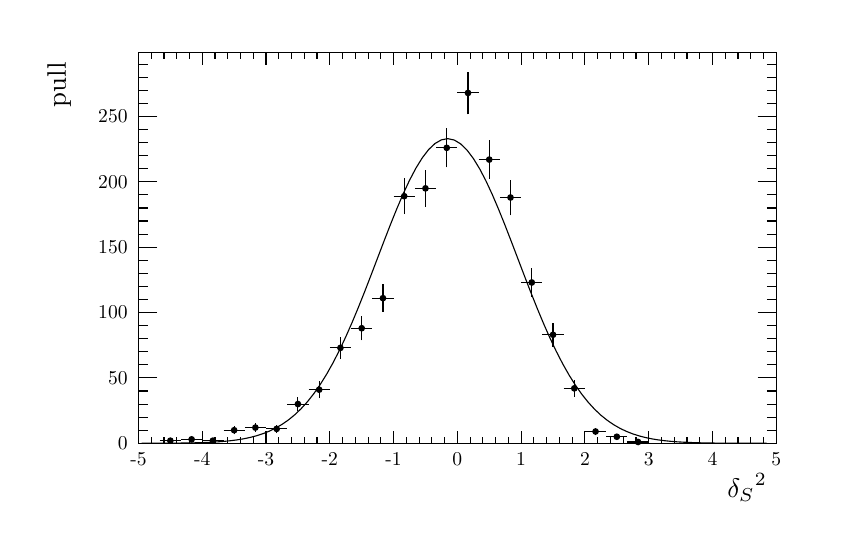
\begin{tikzpicture}
\pgfdeclareplotmark{cross} {
\pgfpathmoveto{\pgfpoint{-0.3\pgfplotmarksize}{\pgfplotmarksize}}
\pgfpathlineto{\pgfpoint{+0.3\pgfplotmarksize}{\pgfplotmarksize}}
\pgfpathlineto{\pgfpoint{+0.3\pgfplotmarksize}{0.3\pgfplotmarksize}}
\pgfpathlineto{\pgfpoint{+1\pgfplotmarksize}{0.3\pgfplotmarksize}}
\pgfpathlineto{\pgfpoint{+1\pgfplotmarksize}{-0.3\pgfplotmarksize}}
\pgfpathlineto{\pgfpoint{+0.3\pgfplotmarksize}{-0.3\pgfplotmarksize}}
\pgfpathlineto{\pgfpoint{+0.3\pgfplotmarksize}{-1.\pgfplotmarksize}}
\pgfpathlineto{\pgfpoint{-0.3\pgfplotmarksize}{-1.\pgfplotmarksize}}
\pgfpathlineto{\pgfpoint{-0.3\pgfplotmarksize}{-0.3\pgfplotmarksize}}
\pgfpathlineto{\pgfpoint{-1.\pgfplotmarksize}{-0.3\pgfplotmarksize}}
\pgfpathlineto{\pgfpoint{-1.\pgfplotmarksize}{0.3\pgfplotmarksize}}
\pgfpathlineto{\pgfpoint{-0.3\pgfplotmarksize}{0.3\pgfplotmarksize}}
\pgfpathclose
\pgfusepathqstroke
}
\pgfdeclareplotmark{cross*} {
\pgfpathmoveto{\pgfpoint{-0.3\pgfplotmarksize}{\pgfplotmarksize}}
\pgfpathlineto{\pgfpoint{+0.3\pgfplotmarksize}{\pgfplotmarksize}}
\pgfpathlineto{\pgfpoint{+0.3\pgfplotmarksize}{0.3\pgfplotmarksize}}
\pgfpathlineto{\pgfpoint{+1\pgfplotmarksize}{0.3\pgfplotmarksize}}
\pgfpathlineto{\pgfpoint{+1\pgfplotmarksize}{-0.3\pgfplotmarksize}}
\pgfpathlineto{\pgfpoint{+0.3\pgfplotmarksize}{-0.3\pgfplotmarksize}}
\pgfpathlineto{\pgfpoint{+0.3\pgfplotmarksize}{-1.\pgfplotmarksize}}
\pgfpathlineto{\pgfpoint{-0.3\pgfplotmarksize}{-1.\pgfplotmarksize}}
\pgfpathlineto{\pgfpoint{-0.3\pgfplotmarksize}{-0.3\pgfplotmarksize}}
\pgfpathlineto{\pgfpoint{-1.\pgfplotmarksize}{-0.3\pgfplotmarksize}}
\pgfpathlineto{\pgfpoint{-1.\pgfplotmarksize}{0.3\pgfplotmarksize}}
\pgfpathlineto{\pgfpoint{-0.3\pgfplotmarksize}{0.3\pgfplotmarksize}}
\pgfpathclose
\pgfusepathqfillstroke
}
\pgfdeclareplotmark{newstar} {
\pgfpathmoveto{\pgfqpoint{0pt}{\pgfplotmarksize}}
\pgfpathlineto{\pgfqpointpolar{44}{0.5\pgfplotmarksize}}
\pgfpathlineto{\pgfqpointpolar{18}{\pgfplotmarksize}}
\pgfpathlineto{\pgfqpointpolar{-20}{0.5\pgfplotmarksize}}
\pgfpathlineto{\pgfqpointpolar{-54}{\pgfplotmarksize}}
\pgfpathlineto{\pgfqpointpolar{-90}{0.5\pgfplotmarksize}}
\pgfpathlineto{\pgfqpointpolar{234}{\pgfplotmarksize}}
\pgfpathlineto{\pgfqpointpolar{198}{0.5\pgfplotmarksize}}
\pgfpathlineto{\pgfqpointpolar{162}{\pgfplotmarksize}}
\pgfpathlineto{\pgfqpointpolar{134}{0.5\pgfplotmarksize}}
\pgfpathclose
\pgfusepathqstroke
}
\pgfdeclareplotmark{newstar*} {
\pgfpathmoveto{\pgfqpoint{0pt}{\pgfplotmarksize}}
\pgfpathlineto{\pgfqpointpolar{44}{0.5\pgfplotmarksize}}
\pgfpathlineto{\pgfqpointpolar{18}{\pgfplotmarksize}}
\pgfpathlineto{\pgfqpointpolar{-20}{0.5\pgfplotmarksize}}
\pgfpathlineto{\pgfqpointpolar{-54}{\pgfplotmarksize}}
\pgfpathlineto{\pgfqpointpolar{-90}{0.5\pgfplotmarksize}}
\pgfpathlineto{\pgfqpointpolar{234}{\pgfplotmarksize}}
\pgfpathlineto{\pgfqpointpolar{198}{0.5\pgfplotmarksize}}
\pgfpathlineto{\pgfqpointpolar{162}{\pgfplotmarksize}}
\pgfpathlineto{\pgfqpointpolar{134}{0.5\pgfplotmarksize}}
\pgfpathclose
\pgfusepathqfillstroke
}
\definecolor{c}{rgb}{1,1,1};
\draw [color=c, fill=c] (0,0) rectangle (10,6.27517);
\draw [color=c, fill=c] (1.4,1.00403) rectangle (9.5,5.96141);
\definecolor{c}{rgb}{0,0,0};
\draw [c] (1.4,1.00403) -- (1.4,5.96141) -- (9.5,5.96141) -- (9.5,1.00403) -- (1.4,1.00403);
\draw [c] (1.805,1.01375) -- (1.805,1.03723);
\draw [c] (1.805,1.03723) -- (1.805,1.06071);
\draw [c] (1.67,1.03723) -- (1.805,1.03723);
\draw [c] (1.805,1.03723) -- (1.94,1.03723);
\foreach \P in {(1.805,1.03723)}{\draw[mark options={color=c,fill=c},mark size=2.402402pt,mark=*,mark size=1pt] plot coordinates {\P};}
\draw [c] (2.075,1.02508) -- (2.075,1.05383);
\draw [c] (2.075,1.05383) -- (2.075,1.08259);
\draw [c] (1.94,1.05383) -- (2.075,1.05383);
\draw [c] (2.075,1.05383) -- (2.21,1.05383);
\foreach \P in {(2.075,1.05383)}{\draw[mark options={color=c,fill=c},mark size=2.402402pt,mark=*,mark size=1pt] plot coordinates {\P};}
\draw [c] (2.345,1.01375) -- (2.345,1.03723);
\draw [c] (2.345,1.03723) -- (2.345,1.06071);
\draw [c] (2.21,1.03723) -- (2.345,1.03723);
\draw [c] (2.345,1.03723) -- (2.48,1.03723);
\foreach \P in {(2.345,1.03723)}{\draw[mark options={color=c,fill=c},mark size=2.402402pt,mark=*,mark size=1pt] plot coordinates {\P};}
\draw [c] (2.615,1.11755) -- (2.615,1.17005);
\draw [c] (2.615,1.17005) -- (2.615,1.22256);
\draw [c] (2.48,1.17005) -- (2.615,1.17005);
\draw [c] (2.615,1.17005) -- (2.75,1.17005);
\foreach \P in {(2.615,1.17005)}{\draw[mark options={color=c,fill=c},mark size=2.402402pt,mark=*,mark size=1pt] plot coordinates {\P};}
\draw [c] (2.885,1.14575) -- (2.885,1.20326);
\draw [c] (2.885,1.20326) -- (2.885,1.26077);
\draw [c] (2.75,1.20326) -- (2.885,1.20326);
\draw [c] (2.885,1.20326) -- (3.02,1.20326);
\foreach \P in {(2.885,1.20326)}{\draw[mark options={color=c,fill=c},mark size=2.402402pt,mark=*,mark size=1pt] plot coordinates {\P};}
\draw [c] (3.155,1.13159) -- (3.155,1.18666);
\draw [c] (3.155,1.18666) -- (3.155,1.24172);
\draw [c] (3.02,1.18666) -- (3.155,1.18666);
\draw [c] (3.155,1.18666) -- (3.29,1.18666);
\foreach \P in {(3.155,1.18666)}{\draw[mark options={color=c,fill=c},mark size=2.402402pt,mark=*,mark size=1pt] plot coordinates {\P};}
\draw [c] (3.425,1.41117) -- (3.425,1.50211);
\draw [c] (3.425,1.50211) -- (3.425,1.59304);
\draw [c] (3.29,1.50211) -- (3.425,1.50211);
\draw [c] (3.425,1.50211) -- (3.56,1.50211);
\foreach \P in {(3.425,1.50211)}{\draw[mark options={color=c,fill=c},mark size=2.402402pt,mark=*,mark size=1pt] plot coordinates {\P};}
\draw [c] (3.695,1.57843) -- (3.695,1.68474);
\draw [c] (3.695,1.68474) -- (3.695,1.79105);
\draw [c] (3.56,1.68474) -- (3.695,1.68474);
\draw [c] (3.695,1.68474) -- (3.83,1.68474);
\foreach \P in {(3.695,1.68474)}{\draw[mark options={color=c,fill=c},mark size=2.402402pt,mark=*,mark size=1pt] plot coordinates {\P};}
\draw [c] (3.965,2.07417) -- (3.965,2.21602);
\draw [c] (3.965,2.21602) -- (3.965,2.35788);
\draw [c] (3.83,2.21602) -- (3.965,2.21602);
\draw [c] (3.965,2.21602) -- (4.1,2.21602);
\foreach \P in {(3.965,2.21602)}{\draw[mark options={color=c,fill=c},mark size=2.402402pt,mark=*,mark size=1pt] plot coordinates {\P};}
\draw [c] (4.235,2.30932) -- (4.235,2.46506);
\draw [c] (4.235,2.46506) -- (4.235,2.62081);
\draw [c] (4.1,2.46506) -- (4.235,2.46506);
\draw [c] (4.235,2.46506) -- (4.37,2.46506);
\foreach \P in {(4.235,2.46506)}{\draw[mark options={color=c,fill=c},mark size=2.402402pt,mark=*,mark size=1pt] plot coordinates {\P};}
\draw [c] (4.505,2.672) -- (4.505,2.84692);
\draw [c] (4.505,2.84692) -- (4.505,3.02184);
\draw [c] (4.37,2.84692) -- (4.505,2.84692);
\draw [c] (4.505,2.84692) -- (4.64,2.84692);
\foreach \P in {(4.505,2.84692)}{\draw[mark options={color=c,fill=c},mark size=2.402402pt,mark=*,mark size=1pt] plot coordinates {\P};}
\draw [c] (4.775,3.91368) -- (4.775,4.14193);
\draw [c] (4.775,4.14193) -- (4.775,4.37018);
\draw [c] (4.64,4.14193) -- (4.775,4.14193);
\draw [c] (4.775,4.14193) -- (4.91,4.14193);
\foreach \P in {(4.775,4.14193)}{\draw[mark options={color=c,fill=c},mark size=2.402402pt,mark=*,mark size=1pt] plot coordinates {\P};}
\draw [c] (5.045,4.00971) -- (5.045,4.24155);
\draw [c] (5.045,4.24155) -- (5.045,4.47339);
\draw [c] (4.91,4.24155) -- (5.045,4.24155);
\draw [c] (5.045,4.24155) -- (5.18,4.24155);
\foreach \P in {(5.045,4.24155)}{\draw[mark options={color=c,fill=c},mark size=2.402402pt,mark=*,mark size=1pt] plot coordinates {\P};}
\draw [c] (5.315,4.50664) -- (5.315,4.75623);
\draw [c] (5.315,4.75623) -- (5.315,5.00583);
\draw [c] (5.18,4.75623) -- (5.315,4.75623);
\draw [c] (5.315,4.75623) -- (5.45,4.75623);
\foreach \P in {(5.315,4.75623)}{\draw[mark options={color=c,fill=c},mark size=2.402402pt,mark=*,mark size=1pt] plot coordinates {\P};}
\draw [c] (5.585,5.18175) -- (5.585,5.45355);
\draw [c] (5.585,5.45355) -- (5.585,5.72534);
\draw [c] (5.45,5.45355) -- (5.585,5.45355);
\draw [c] (5.585,5.45355) -- (5.72,5.45355);
\foreach \P in {(5.585,5.45355)}{\draw[mark options={color=c,fill=c},mark size=2.402402pt,mark=*,mark size=1pt] plot coordinates {\P};}
\draw [c] (5.855,4.36224) -- (5.855,4.60681);
\draw [c] (5.855,4.60681) -- (5.855,4.85138);
\draw [c] (5.72,4.60681) -- (5.855,4.60681);
\draw [c] (5.855,4.60681) -- (5.99,4.60681);
\foreach \P in {(5.855,4.60681)}{\draw[mark options={color=c,fill=c},mark size=2.402402pt,mark=*,mark size=1pt] plot coordinates {\P};}
\draw [c] (6.125,3.89769) -- (6.125,4.12533);
\draw [c] (6.125,4.12533) -- (6.125,4.35298);
\draw [c] (5.99,4.12533) -- (6.125,4.12533);
\draw [c] (6.125,4.12533) -- (6.26,4.12533);
\foreach \P in {(6.125,4.12533)}{\draw[mark options={color=c,fill=c},mark size=2.402402pt,mark=*,mark size=1pt] plot coordinates {\P};}
\draw [c] (6.395,2.86202) -- (6.395,3.04616);
\draw [c] (6.395,3.04616) -- (6.395,3.23029);
\draw [c] (6.26,3.04616) -- (6.395,3.04616);
\draw [c] (6.395,3.04616) -- (6.53,3.04616);
\foreach \P in {(6.395,3.04616)}{\draw[mark options={color=c,fill=c},mark size=2.402402pt,mark=*,mark size=1pt] plot coordinates {\P};}
\draw [c] (6.665,2.23079) -- (6.665,2.38205);
\draw [c] (6.665,2.38205) -- (6.665,2.53331);
\draw [c] (6.53,2.38205) -- (6.665,2.38205);
\draw [c] (6.665,2.38205) -- (6.8,2.38205);
\foreach \P in {(6.665,2.38205)}{\draw[mark options={color=c,fill=c},mark size=2.402402pt,mark=*,mark size=1pt] plot coordinates {\P};}
\draw [c] (6.935,1.59374) -- (6.935,1.70134);
\draw [c] (6.935,1.70134) -- (6.935,1.80894);
\draw [c] (6.8,1.70134) -- (6.935,1.70134);
\draw [c] (6.935,1.70134) -- (7.07,1.70134);
\foreach \P in {(6.935,1.70134)}{\draw[mark options={color=c,fill=c},mark size=2.402402pt,mark=*,mark size=1pt] plot coordinates {\P};}
\draw [c] (7.205,1.10364) -- (7.205,1.15345);
\draw [c] (7.205,1.15345) -- (7.205,1.20326);
\draw [c] (7.07,1.15345) -- (7.205,1.15345);
\draw [c] (7.205,1.15345) -- (7.34,1.15345);
\foreach \P in {(7.205,1.15345)}{\draw[mark options={color=c,fill=c},mark size=2.402402pt,mark=*,mark size=1pt] plot coordinates {\P};}
\draw [c] (7.475,1.04992) -- (7.475,1.08704);
\draw [c] (7.475,1.08704) -- (7.475,1.12416);
\draw [c] (7.34,1.08704) -- (7.475,1.08704);
\draw [c] (7.475,1.08704) -- (7.61,1.08704);
\foreach \P in {(7.475,1.08704)}{\draw[mark options={color=c,fill=c},mark size=2.402402pt,mark=*,mark size=1pt] plot coordinates {\P};}
\draw [c] (7.745,1.00403) -- (7.745,1.02063);
\draw [c] (7.745,1.02063) -- (7.745,1.03723);
\draw [c] (7.61,1.02063) -- (7.745,1.02063);
\draw [c] (7.745,1.02063) -- (7.88,1.02063);
\foreach \P in {(7.745,1.02063)}{\draw[mark options={color=c,fill=c},mark size=2.402402pt,mark=*,mark size=1pt] plot coordinates {\P};}
\draw [c,line width=0.4] (1.4405,1.00403) -- (1.5215,1.00403) -- (1.6025,1.00466) -- (1.6835,1.00495) -- (1.7645,1.00536) -- (1.8455,1.00593) -- (1.9265,1.00673) -- (2.0075,1.00783) -- (2.0885,1.00934) -- (2.1695,1.01139) -- (2.2505,1.01414) --
 (2.3315,1.0178) -- (2.4125,1.02264) -- (2.4935,1.02896) -- (2.5745,1.03716) -- (2.6555,1.0477) -- (2.7365,1.06112) -- (2.8175,1.07805) -- (2.8985,1.0992) -- (2.9795,1.1254) -- (3.0605,1.15753) -- (3.1415,1.19658) -- (3.2225,1.24357) --
 (3.3035,1.29959) -- (3.3845,1.36571) -- (3.4655,1.44298) -- (3.5465,1.53238) -- (3.6275,1.63477) -- (3.7085,1.7508) -- (3.7895,1.88093) -- (3.8705,2.02526) -- (3.9515,2.18358) -- (4.0325,2.35525) -- (4.1135,2.53919) -- (4.1945,2.73383) --
 (4.2755,2.93713) -- (4.3565,3.14658) -- (4.4375,3.35921) -- (4.5185,3.57166) -- (4.5995,3.78028) -- (4.6805,3.98119) -- (4.7615,4.1704) -- (4.8425,4.34397) -- (4.9235,4.4981) -- (5.0045,4.62931) -- (5.0855,4.73454) -- (5.1665,4.81128) --
 (5.2475,4.85767) -- (5.3285,4.87258) -- (5.4095,4.85563);
\draw [c,line width=0.4] (5.4095,4.85563) -- (5.4905,4.80725) -- (5.5715,4.72862) -- (5.6525,4.62164) -- (5.7335,4.48887) -- (5.8145,4.33338) -- (5.8955,4.15869) -- (5.9765,3.96861) -- (6.0575,3.76709) -- (6.1385,3.55811) -- (6.2195,3.34554) --
 (6.3005,3.13302) -- (6.3815,2.92388) -- (6.4625,2.72106) -- (6.5435,2.52705) -- (6.6245,2.34386) -- (6.7055,2.17302) -- (6.7865,2.01558) -- (6.8675,1.87216) -- (6.9485,1.74294) -- (7.0295,1.6278) -- (7.1105,1.52626) -- (7.1915,1.43767) --
 (7.2725,1.36114) -- (7.3535,1.2957) -- (7.4345,1.2403) -- (7.5155,1.19385) -- (7.5965,1.15527) -- (7.6775,1.12355) -- (7.7585,1.0977) -- (7.8395,1.07684) -- (7.9205,1.06016) -- (8.0015,1.04695) -- (8.0825,1.03657) -- (8.1635,1.0285) --
 (8.2445,1.02228) -- (8.3255,1.01753) -- (8.4065,1.01394) -- (8.4875,1.01124) -- (8.5685,1.00923) -- (8.6495,1.00775) -- (8.7305,1.00667) -- (8.8115,1.00589) -- (8.8925,1.00533) -- (8.9735,1.00493) -- (9.0545,1.00465) -- (9.1355,1.00403) --
 (9.2165,1.00403) -- (9.2975,1.00403) -- (9.3785,1.00403);
\draw [c,line width=0.4] (9.3785,1.00403) -- (9.4595,1.00403);
\draw [c,line width=0.4] (1.4,1.00403) -- (9.5,1.00403);
\draw [anchor= east] (9.5,0.441772) node[scale=0.96888, rotate=0]{${\delta_\text{S}}^2$};
\draw [c,line width=0.4] (1.4,1.15651) -- (1.4,1.00403);
\draw [c,line width=0.4] (1.562,1.08027) -- (1.562,1.00403);
\draw [c,line width=0.4] (1.724,1.08027) -- (1.724,1.00403);
\draw [c,line width=0.4] (1.886,1.08027) -- (1.886,1.00403);
\draw [c,line width=0.4] (2.048,1.08027) -- (2.048,1.00403);
\draw [c,line width=0.4] (2.21,1.15651) -- (2.21,1.00403);
\draw [c,line width=0.4] (2.372,1.08027) -- (2.372,1.00403);
\draw [c,line width=0.4] (2.534,1.08027) -- (2.534,1.00403);
\draw [c,line width=0.4] (2.696,1.08027) -- (2.696,1.00403);
\draw [c,line width=0.4] (2.858,1.08027) -- (2.858,1.00403);
\draw [c,line width=0.4] (3.02,1.15651) -- (3.02,1.00403);
\draw [c,line width=0.4] (3.182,1.08027) -- (3.182,1.00403);
\draw [c,line width=0.4] (3.344,1.08027) -- (3.344,1.00403);
\draw [c,line width=0.4] (3.506,1.08027) -- (3.506,1.00403);
\draw [c,line width=0.4] (3.668,1.08027) -- (3.668,1.00403);
\draw [c,line width=0.4] (3.83,1.15651) -- (3.83,1.00403);
\draw [c,line width=0.4] (3.992,1.08027) -- (3.992,1.00403);
\draw [c,line width=0.4] (4.154,1.08027) -- (4.154,1.00403);
\draw [c,line width=0.4] (4.316,1.08027) -- (4.316,1.00403);
\draw [c,line width=0.4] (4.478,1.08027) -- (4.478,1.00403);
\draw [c,line width=0.4] (4.64,1.15651) -- (4.64,1.00403);
\draw [c,line width=0.4] (4.802,1.08027) -- (4.802,1.00403);
\draw [c,line width=0.4] (4.964,1.08027) -- (4.964,1.00403);
\draw [c,line width=0.4] (5.126,1.08027) -- (5.126,1.00403);
\draw [c,line width=0.4] (5.288,1.08027) -- (5.288,1.00403);
\draw [c,line width=0.4] (5.45,1.15651) -- (5.45,1.00403);
\draw [c,line width=0.4] (5.612,1.08027) -- (5.612,1.00403);
\draw [c,line width=0.4] (5.774,1.08027) -- (5.774,1.00403);
\draw [c,line width=0.4] (5.936,1.08027) -- (5.936,1.00403);
\draw [c,line width=0.4] (6.098,1.08027) -- (6.098,1.00403);
\draw [c,line width=0.4] (6.26,1.15651) -- (6.26,1.00403);
\draw [c,line width=0.4] (6.422,1.08027) -- (6.422,1.00403);
\draw [c,line width=0.4] (6.584,1.08027) -- (6.584,1.00403);
\draw [c,line width=0.4] (6.746,1.08027) -- (6.746,1.00403);
\draw [c,line width=0.4] (6.908,1.08027) -- (6.908,1.00403);
\draw [c,line width=0.4] (7.07,1.15651) -- (7.07,1.00403);
\draw [c,line width=0.4] (7.232,1.08027) -- (7.232,1.00403);
\draw [c,line width=0.4] (7.394,1.08027) -- (7.394,1.00403);
\draw [c,line width=0.4] (7.556,1.08027) -- (7.556,1.00403);
\draw [c,line width=0.4] (7.718,1.08027) -- (7.718,1.00403);
\draw [c,line width=0.4] (7.88,1.15651) -- (7.88,1.00403);
\draw [c,line width=0.4] (8.042,1.08027) -- (8.042,1.00403);
\draw [c,line width=0.4] (8.204,1.08027) -- (8.204,1.00403);
\draw [c,line width=0.4] (8.366,1.08027) -- (8.366,1.00403);
\draw [c,line width=0.4] (8.528,1.08027) -- (8.528,1.00403);
\draw [c,line width=0.4] (8.69,1.15651) -- (8.69,1.00403);
\draw [c,line width=0.4] (8.852,1.08027) -- (8.852,1.00403);
\draw [c,line width=0.4] (9.014,1.08027) -- (9.014,1.00403);
\draw [c,line width=0.4] (9.176,1.08027) -- (9.176,1.00403);
\draw [c,line width=0.4] (9.338,1.08027) -- (9.338,1.00403);
\draw [c,line width=0.4] (9.5,1.15651) -- (9.5,1.00403);
\draw [anchor=base] (1.4,0.721644) node[scale=0.708027, rotate=0]{-5};
\draw [anchor=base] (2.21,0.721644) node[scale=0.708027, rotate=0]{-4};
\draw [anchor=base] (3.02,0.721644) node[scale=0.708027, rotate=0]{-3};
\draw [anchor=base] (3.83,0.721644) node[scale=0.708027, rotate=0]{-2};
\draw [anchor=base] (4.64,0.721644) node[scale=0.708027, rotate=0]{-1};
\draw [anchor=base] (5.45,0.721644) node[scale=0.708027, rotate=0]{0};
\draw [anchor=base] (6.26,0.721644) node[scale=0.708027, rotate=0]{1};
\draw [anchor=base] (7.07,0.721644) node[scale=0.708027, rotate=0]{2};
\draw [anchor=base] (7.88,0.721644) node[scale=0.708027, rotate=0]{3};
\draw [anchor=base] (8.69,0.721644) node[scale=0.708027, rotate=0]{4};
\draw [anchor=base] (9.5,0.721644) node[scale=0.708027, rotate=0]{5};
\draw [c,line width=0.4] (1.4,5.96141) -- (9.5,5.96141);
\draw [c,line width=0.4] (1.4,5.80892) -- (1.4,5.96141);
\draw [c,line width=0.4] (1.562,5.88517) -- (1.562,5.96141);
\draw [c,line width=0.4] (1.724,5.88517) -- (1.724,5.96141);
\draw [c,line width=0.4] (1.886,5.88517) -- (1.886,5.96141);
\draw [c,line width=0.4] (2.048,5.88517) -- (2.048,5.96141);
\draw [c,line width=0.4] (2.21,5.80892) -- (2.21,5.96141);
\draw [c,line width=0.4] (2.372,5.88517) -- (2.372,5.96141);
\draw [c,line width=0.4] (2.534,5.88517) -- (2.534,5.96141);
\draw [c,line width=0.4] (2.696,5.88517) -- (2.696,5.96141);
\draw [c,line width=0.4] (2.858,5.88517) -- (2.858,5.96141);
\draw [c,line width=0.4] (3.02,5.80892) -- (3.02,5.96141);
\draw [c,line width=0.4] (3.182,5.88517) -- (3.182,5.96141);
\draw [c,line width=0.4] (3.344,5.88517) -- (3.344,5.96141);
\draw [c,line width=0.4] (3.506,5.88517) -- (3.506,5.96141);
\draw [c,line width=0.4] (3.668,5.88517) -- (3.668,5.96141);
\draw [c,line width=0.4] (3.83,5.80892) -- (3.83,5.96141);
\draw [c,line width=0.4] (3.992,5.88517) -- (3.992,5.96141);
\draw [c,line width=0.4] (4.154,5.88517) -- (4.154,5.96141);
\draw [c,line width=0.4] (4.316,5.88517) -- (4.316,5.96141);
\draw [c,line width=0.4] (4.478,5.88517) -- (4.478,5.96141);
\draw [c,line width=0.4] (4.64,5.80892) -- (4.64,5.96141);
\draw [c,line width=0.4] (4.802,5.88517) -- (4.802,5.96141);
\draw [c,line width=0.4] (4.964,5.88517) -- (4.964,5.96141);
\draw [c,line width=0.4] (5.126,5.88517) -- (5.126,5.96141);
\draw [c,line width=0.4] (5.288,5.88517) -- (5.288,5.96141);
\draw [c,line width=0.4] (5.45,5.80892) -- (5.45,5.96141);
\draw [c,line width=0.4] (5.612,5.88517) -- (5.612,5.96141);
\draw [c,line width=0.4] (5.774,5.88517) -- (5.774,5.96141);
\draw [c,line width=0.4] (5.936,5.88517) -- (5.936,5.96141);
\draw [c,line width=0.4] (6.098,5.88517) -- (6.098,5.96141);
\draw [c,line width=0.4] (6.26,5.80892) -- (6.26,5.96141);
\draw [c,line width=0.4] (6.422,5.88517) -- (6.422,5.96141);
\draw [c,line width=0.4] (6.584,5.88517) -- (6.584,5.96141);
\draw [c,line width=0.4] (6.746,5.88517) -- (6.746,5.96141);
\draw [c,line width=0.4] (6.908,5.88517) -- (6.908,5.96141);
\draw [c,line width=0.4] (7.07,5.80892) -- (7.07,5.96141);
\draw [c,line width=0.4] (7.232,5.88517) -- (7.232,5.96141);
\draw [c,line width=0.4] (7.394,5.88517) -- (7.394,5.96141);
\draw [c,line width=0.4] (7.556,5.88517) -- (7.556,5.96141);
\draw [c,line width=0.4] (7.718,5.88517) -- (7.718,5.96141);
\draw [c,line width=0.4] (7.88,5.80892) -- (7.88,5.96141);
\draw [c,line width=0.4] (8.042,5.88517) -- (8.042,5.96141);
\draw [c,line width=0.4] (8.204,5.88517) -- (8.204,5.96141);
\draw [c,line width=0.4] (8.366,5.88517) -- (8.366,5.96141);
\draw [c,line width=0.4] (8.528,5.88517) -- (8.528,5.96141);
\draw [c,line width=0.4] (8.69,5.80892) -- (8.69,5.96141);
\draw [c,line width=0.4] (8.852,5.88517) -- (8.852,5.96141);
\draw [c,line width=0.4] (9.014,5.88517) -- (9.014,5.96141);
\draw [c,line width=0.4] (9.176,5.88517) -- (9.176,5.96141);
\draw [c,line width=0.4] (9.338,5.88517) -- (9.338,5.96141);
\draw [c,line width=0.4] (9.5,5.80892) -- (9.5,5.96141);
\draw [c,line width=0.4] (1.4,1.00403) -- (1.4,5.96141);
\draw [anchor= east] (0.392,5.96141) node[scale=0.96888, rotate=90]{pull};
\draw [c,line width=0.4] (1.637,1.00403) -- (1.4,1.00403);
\draw [c,line width=0.4] (1.5185,1.17005) -- (1.4,1.17005);
\draw [c,line width=0.4] (1.5185,1.33608) -- (1.4,1.33608);
\draw [c,line width=0.4] (1.5185,1.50211) -- (1.4,1.50211);
\draw [c,line width=0.4] (1.5185,1.66813) -- (1.4,1.66813);
\draw [c,line width=0.4] (1.637,1.83416) -- (1.4,1.83416);
\draw [c,line width=0.4] (1.5185,2.00019) -- (1.4,2.00019);
\draw [c,line width=0.4] (1.5185,2.16621) -- (1.4,2.16621);
\draw [c,line width=0.4] (1.5185,2.33224) -- (1.4,2.33224);
\draw [c,line width=0.4] (1.5185,2.49827) -- (1.4,2.49827);
\draw [c,line width=0.4] (1.637,2.6643) -- (1.4,2.6643);
\draw [c,line width=0.4] (1.5185,2.83032) -- (1.4,2.83032);
\draw [c,line width=0.4] (1.5185,2.99635) -- (1.4,2.99635);
\draw [c,line width=0.4] (1.5185,3.16238) -- (1.4,3.16238);
\draw [c,line width=0.4] (1.5185,3.3284) -- (1.4,3.3284);
\draw [c,line width=0.4] (1.637,3.49443) -- (1.4,3.49443);
\draw [c,line width=0.4] (1.5185,3.66046) -- (1.4,3.66046);
\draw [c,line width=0.4] (1.5185,3.82648) -- (1.4,3.82648);
\draw [c,line width=0.4] (1.5185,3.99251) -- (1.4,3.99251);
\draw [c,line width=0.4] (1.5185,4.15854) -- (1.4,4.15854);
\draw [c,line width=0.4] (1.637,4.32456) -- (1.4,4.32456);
\draw [c,line width=0.4] (1.5185,4.49059) -- (1.4,4.49059);
\draw [c,line width=0.4] (1.5185,4.65662) -- (1.4,4.65662);
\draw [c,line width=0.4] (1.5185,4.82264) -- (1.4,4.82264);
\draw [c,line width=0.4] (1.5185,4.98867) -- (1.4,4.98867);
\draw [c,line width=0.4] (1.637,5.1547) -- (1.4,5.1547);
\draw [c,line width=0.4] (1.637,5.1547) -- (1.4,5.1547);
\draw [c,line width=0.4] (1.5185,5.32072) -- (1.4,5.32072);
\draw [c,line width=0.4] (1.5185,5.48675) -- (1.4,5.48675);
\draw [c,line width=0.4] (1.5185,5.65278) -- (1.4,5.65278);
\draw [c,line width=0.4] (1.5185,5.81881) -- (1.4,5.81881);
\draw [anchor= east] (1.35,1.00403) node[scale=0.708027, rotate=0]{0};
\draw [anchor= east] (1.35,1.83416) node[scale=0.708027, rotate=0]{50};
\draw [anchor= east] (1.35,2.6643) node[scale=0.708027, rotate=0]{100};
\draw [anchor= east] (1.35,3.49443) node[scale=0.708027, rotate=0]{150};
\draw [anchor= east] (1.35,4.32456) node[scale=0.708027, rotate=0]{200};
\draw [anchor= east] (1.35,5.1547) node[scale=0.708027, rotate=0]{250};
\draw [c,line width=0.4] (9.5,1.00403) -- (9.5,5.96141);
\draw [c,line width=0.4] (9.263,1.00403) -- (9.5,1.00403);
\draw [c,line width=0.4] (9.3815,1.17005) -- (9.5,1.17005);
\draw [c,line width=0.4] (9.3815,1.33608) -- (9.5,1.33608);
\draw [c,line width=0.4] (9.3815,1.50211) -- (9.5,1.50211);
\draw [c,line width=0.4] (9.3815,1.66813) -- (9.5,1.66813);
\draw [c,line width=0.4] (9.263,1.83416) -- (9.5,1.83416);
\draw [c,line width=0.4] (9.3815,2.00019) -- (9.5,2.00019);
\draw [c,line width=0.4] (9.3815,2.16621) -- (9.5,2.16621);
\draw [c,line width=0.4] (9.3815,2.33224) -- (9.5,2.33224);
\draw [c,line width=0.4] (9.3815,2.49827) -- (9.5,2.49827);
\draw [c,line width=0.4] (9.263,2.6643) -- (9.5,2.6643);
\draw [c,line width=0.4] (9.3815,2.83032) -- (9.5,2.83032);
\draw [c,line width=0.4] (9.3815,2.99635) -- (9.5,2.99635);
\draw [c,line width=0.4] (9.3815,3.16238) -- (9.5,3.16238);
\draw [c,line width=0.4] (9.3815,3.3284) -- (9.5,3.3284);
\draw [c,line width=0.4] (9.263,3.49443) -- (9.5,3.49443);
\draw [c,line width=0.4] (9.3815,3.66046) -- (9.5,3.66046);
\draw [c,line width=0.4] (9.3815,3.82648) -- (9.5,3.82648);
\draw [c,line width=0.4] (9.3815,3.99251) -- (9.5,3.99251);
\draw [c,line width=0.4] (9.3815,4.15854) -- (9.5,4.15854);
\draw [c,line width=0.4] (9.263,4.32456) -- (9.5,4.32456);
\draw [c,line width=0.4] (9.3815,4.49059) -- (9.5,4.49059);
\draw [c,line width=0.4] (9.3815,4.65662) -- (9.5,4.65662);
\draw [c,line width=0.4] (9.3815,4.82264) -- (9.5,4.82264);
\draw [c,line width=0.4] (9.3815,4.98867) -- (9.5,4.98867);
\draw [c,line width=0.4] (9.263,5.1547) -- (9.5,5.1547);
\draw [c,line width=0.4] (9.263,5.1547) -- (9.5,5.1547);
\draw [c,line width=0.4] (9.3815,5.32072) -- (9.5,5.32072);
\draw [c,line width=0.4] (9.3815,5.48675) -- (9.5,5.48675);
\draw [c,line width=0.4] (9.3815,5.65278) -- (9.5,5.65278);
\draw [c,line width=0.4] (9.3815,5.81881) -- (9.5,5.81881);
\end{tikzpicture}
}
    \caption{}
    \label{pull_ASPhase_bin2}
  \end{subfigure}
  \begin{subfigure}{0.5\textwidth}
    \tikzsetnextfilename{pull_ASMag2_bin3}
    \scalebox{0.60}{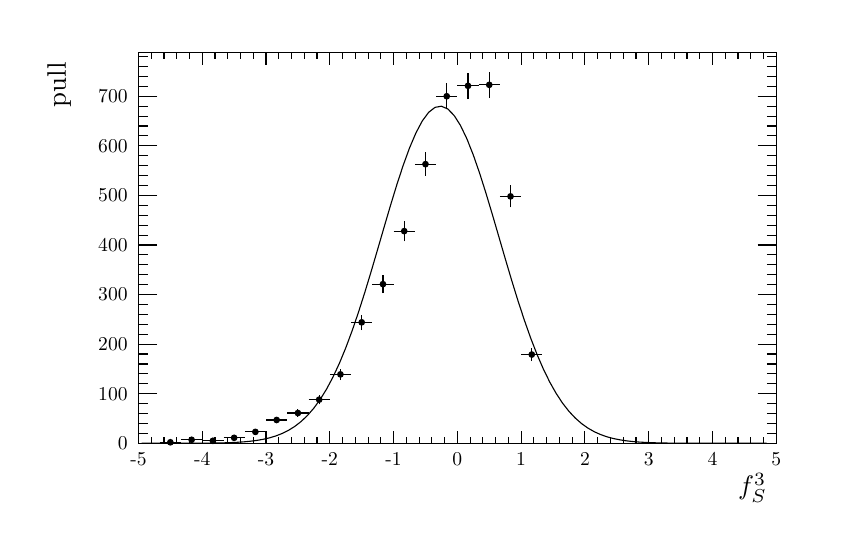
\begin{tikzpicture}
\pgfdeclareplotmark{cross} {
\pgfpathmoveto{\pgfpoint{-0.3\pgfplotmarksize}{\pgfplotmarksize}}
\pgfpathlineto{\pgfpoint{+0.3\pgfplotmarksize}{\pgfplotmarksize}}
\pgfpathlineto{\pgfpoint{+0.3\pgfplotmarksize}{0.3\pgfplotmarksize}}
\pgfpathlineto{\pgfpoint{+1\pgfplotmarksize}{0.3\pgfplotmarksize}}
\pgfpathlineto{\pgfpoint{+1\pgfplotmarksize}{-0.3\pgfplotmarksize}}
\pgfpathlineto{\pgfpoint{+0.3\pgfplotmarksize}{-0.3\pgfplotmarksize}}
\pgfpathlineto{\pgfpoint{+0.3\pgfplotmarksize}{-1.\pgfplotmarksize}}
\pgfpathlineto{\pgfpoint{-0.3\pgfplotmarksize}{-1.\pgfplotmarksize}}
\pgfpathlineto{\pgfpoint{-0.3\pgfplotmarksize}{-0.3\pgfplotmarksize}}
\pgfpathlineto{\pgfpoint{-1.\pgfplotmarksize}{-0.3\pgfplotmarksize}}
\pgfpathlineto{\pgfpoint{-1.\pgfplotmarksize}{0.3\pgfplotmarksize}}
\pgfpathlineto{\pgfpoint{-0.3\pgfplotmarksize}{0.3\pgfplotmarksize}}
\pgfpathclose
\pgfusepathqstroke
}
\pgfdeclareplotmark{cross*} {
\pgfpathmoveto{\pgfpoint{-0.3\pgfplotmarksize}{\pgfplotmarksize}}
\pgfpathlineto{\pgfpoint{+0.3\pgfplotmarksize}{\pgfplotmarksize}}
\pgfpathlineto{\pgfpoint{+0.3\pgfplotmarksize}{0.3\pgfplotmarksize}}
\pgfpathlineto{\pgfpoint{+1\pgfplotmarksize}{0.3\pgfplotmarksize}}
\pgfpathlineto{\pgfpoint{+1\pgfplotmarksize}{-0.3\pgfplotmarksize}}
\pgfpathlineto{\pgfpoint{+0.3\pgfplotmarksize}{-0.3\pgfplotmarksize}}
\pgfpathlineto{\pgfpoint{+0.3\pgfplotmarksize}{-1.\pgfplotmarksize}}
\pgfpathlineto{\pgfpoint{-0.3\pgfplotmarksize}{-1.\pgfplotmarksize}}
\pgfpathlineto{\pgfpoint{-0.3\pgfplotmarksize}{-0.3\pgfplotmarksize}}
\pgfpathlineto{\pgfpoint{-1.\pgfplotmarksize}{-0.3\pgfplotmarksize}}
\pgfpathlineto{\pgfpoint{-1.\pgfplotmarksize}{0.3\pgfplotmarksize}}
\pgfpathlineto{\pgfpoint{-0.3\pgfplotmarksize}{0.3\pgfplotmarksize}}
\pgfpathclose
\pgfusepathqfillstroke
}
\pgfdeclareplotmark{newstar} {
\pgfpathmoveto{\pgfqpoint{0pt}{\pgfplotmarksize}}
\pgfpathlineto{\pgfqpointpolar{44}{0.5\pgfplotmarksize}}
\pgfpathlineto{\pgfqpointpolar{18}{\pgfplotmarksize}}
\pgfpathlineto{\pgfqpointpolar{-20}{0.5\pgfplotmarksize}}
\pgfpathlineto{\pgfqpointpolar{-54}{\pgfplotmarksize}}
\pgfpathlineto{\pgfqpointpolar{-90}{0.5\pgfplotmarksize}}
\pgfpathlineto{\pgfqpointpolar{234}{\pgfplotmarksize}}
\pgfpathlineto{\pgfqpointpolar{198}{0.5\pgfplotmarksize}}
\pgfpathlineto{\pgfqpointpolar{162}{\pgfplotmarksize}}
\pgfpathlineto{\pgfqpointpolar{134}{0.5\pgfplotmarksize}}
\pgfpathclose
\pgfusepathqstroke
}
\pgfdeclareplotmark{newstar*} {
\pgfpathmoveto{\pgfqpoint{0pt}{\pgfplotmarksize}}
\pgfpathlineto{\pgfqpointpolar{44}{0.5\pgfplotmarksize}}
\pgfpathlineto{\pgfqpointpolar{18}{\pgfplotmarksize}}
\pgfpathlineto{\pgfqpointpolar{-20}{0.5\pgfplotmarksize}}
\pgfpathlineto{\pgfqpointpolar{-54}{\pgfplotmarksize}}
\pgfpathlineto{\pgfqpointpolar{-90}{0.5\pgfplotmarksize}}
\pgfpathlineto{\pgfqpointpolar{234}{\pgfplotmarksize}}
\pgfpathlineto{\pgfqpointpolar{198}{0.5\pgfplotmarksize}}
\pgfpathlineto{\pgfqpointpolar{162}{\pgfplotmarksize}}
\pgfpathlineto{\pgfqpointpolar{134}{0.5\pgfplotmarksize}}
\pgfpathclose
\pgfusepathqfillstroke
}
\definecolor{c}{rgb}{1,1,1};
\draw [color=c, fill=c] (0,0) rectangle (10,6.27517);
\draw [color=c, fill=c] (1.4,1.00403) rectangle (9.5,5.96141);
\definecolor{c}{rgb}{0,0,0};
\draw [c] (1.4,1.00403) -- (1.4,5.96141) -- (9.5,5.96141) -- (9.5,1.00403) -- (1.4,1.00403);
\draw [c] (1.805,1.00771) -- (1.805,1.01662);
\draw [c] (1.805,1.01662) -- (1.805,1.02552);
\draw [c] (1.67,1.01662) -- (1.805,1.01662);
\draw [c] (1.805,1.01662) -- (1.94,1.01662);
\foreach \P in {(1.805,1.01662)}{\draw[mark options={color=c,fill=c},mark size=2.402402pt,mark=*,mark size=1pt] plot coordinates {\P};}
\draw [c] (2.075,1.03144) -- (2.075,1.0481);
\draw [c] (2.075,1.0481) -- (2.075,1.06476);
\draw [c] (1.94,1.0481) -- (2.075,1.0481);
\draw [c] (2.075,1.0481) -- (2.21,1.0481);
\foreach \P in {(2.075,1.0481)}{\draw[mark options={color=c,fill=c},mark size=2.402402pt,mark=*,mark size=1pt] plot coordinates {\P};}
\draw [c] (2.345,1.02143) -- (2.345,1.03551);
\draw [c] (2.345,1.03551) -- (2.345,1.04959);
\draw [c] (2.21,1.03551) -- (2.345,1.03551);
\draw [c] (2.345,1.03551) -- (2.48,1.03551);
\foreach \P in {(2.345,1.03551)}{\draw[mark options={color=c,fill=c},mark size=2.402402pt,mark=*,mark size=1pt] plot coordinates {\P};}
\draw [c] (2.615,1.0524) -- (2.615,1.07328);
\draw [c] (2.615,1.07328) -- (2.615,1.09416);
\draw [c] (2.48,1.07328) -- (2.615,1.07328);
\draw [c] (2.615,1.07328) -- (2.75,1.07328);
\foreach \P in {(2.615,1.07328)}{\draw[mark options={color=c,fill=c},mark size=2.402402pt,mark=*,mark size=1pt] plot coordinates {\P};}
\draw [c] (2.885,1.11864) -- (2.885,1.14884);
\draw [c] (2.885,1.14884) -- (2.885,1.17903);
\draw [c] (2.75,1.14884) -- (2.885,1.14884);
\draw [c] (2.885,1.14884) -- (3.02,1.14884);
\foreach \P in {(2.885,1.14884)}{\draw[mark options={color=c,fill=c},mark size=2.402402pt,mark=*,mark size=1pt] plot coordinates {\P};}
\draw [c] (3.155,1.25678) -- (3.155,1.29994);
\draw [c] (3.155,1.29994) -- (3.155,1.3431);
\draw [c] (3.02,1.29994) -- (3.155,1.29994);
\draw [c] (3.155,1.29994) -- (3.29,1.29994);
\foreach \P in {(3.155,1.29994)}{\draw[mark options={color=c,fill=c},mark size=2.402402pt,mark=*,mark size=1pt] plot coordinates {\P};}
\draw [c] (3.425,1.33891) -- (3.425,1.38808);
\draw [c] (3.425,1.38808) -- (3.425,1.43726);
\draw [c] (3.29,1.38808) -- (3.425,1.38808);
\draw [c] (3.425,1.38808) -- (3.56,1.38808);
\foreach \P in {(3.425,1.38808)}{\draw[mark options={color=c,fill=c},mark size=2.402402pt,mark=*,mark size=1pt] plot coordinates {\P};}
\draw [c] (3.695,1.49901) -- (3.695,1.55808);
\draw [c] (3.695,1.55808) -- (3.695,1.61714);
\draw [c] (3.56,1.55808) -- (3.695,1.55808);
\draw [c] (3.695,1.55808) -- (3.83,1.55808);
\foreach \P in {(3.695,1.55808)}{\draw[mark options={color=c,fill=c},mark size=2.402402pt,mark=*,mark size=1pt] plot coordinates {\P};}
\draw [c] (3.965,1.80495) -- (3.965,1.87917);
\draw [c] (3.965,1.87917) -- (3.965,1.9534);
\draw [c] (3.83,1.87917) -- (3.965,1.87917);
\draw [c] (3.965,1.87917) -- (4.1,1.87917);
\foreach \P in {(3.965,1.87917)}{\draw[mark options={color=c,fill=c},mark size=2.402402pt,mark=*,mark size=1pt] plot coordinates {\P};}
\draw [c] (4.235,2.44191) -- (4.235,2.54026);
\draw [c] (4.235,2.54026) -- (4.235,2.6386);
\draw [c] (4.1,2.54026) -- (4.235,2.54026);
\draw [c] (4.235,2.54026) -- (4.37,2.54026);
\foreach \P in {(4.235,2.54026)}{\draw[mark options={color=c,fill=c},mark size=2.402402pt,mark=*,mark size=1pt] plot coordinates {\P};}
\draw [c] (4.505,2.91225) -- (4.505,3.02505);
\draw [c] (4.505,3.02505) -- (4.505,3.13785);
\draw [c] (4.37,3.02505) -- (4.505,3.02505);
\draw [c] (4.505,3.02505) -- (4.64,3.02505);
\foreach \P in {(4.505,3.02505)}{\draw[mark options={color=c,fill=c},mark size=2.402402pt,mark=*,mark size=1pt] plot coordinates {\P};}
\draw [c] (4.775,3.56847) -- (4.775,3.69872);
\draw [c] (4.775,3.69872) -- (4.775,3.82898);
\draw [c] (4.64,3.69872) -- (4.775,3.69872);
\draw [c] (4.775,3.69872) -- (4.91,3.69872);
\foreach \P in {(4.775,3.69872)}{\draw[mark options={color=c,fill=c},mark size=2.402402pt,mark=*,mark size=1pt] plot coordinates {\P};}
\draw [c] (5.045,4.3993) -- (5.045,4.54869);
\draw [c] (5.045,4.54869) -- (5.045,4.69808);
\draw [c] (4.91,4.54869) -- (5.045,4.54869);
\draw [c] (5.045,4.54869) -- (5.18,4.54869);
\foreach \P in {(5.045,4.54869)}{\draw[mark options={color=c,fill=c},mark size=2.402402pt,mark=*,mark size=1pt] plot coordinates {\P};}
\draw [c] (5.315,5.24467) -- (5.315,5.41124);
\draw [c] (5.315,5.41124) -- (5.315,5.57782);
\draw [c] (5.18,5.41124) -- (5.315,5.41124);
\draw [c] (5.315,5.41124) -- (5.45,5.41124);
\foreach \P in {(5.315,5.41124)}{\draw[mark options={color=c,fill=c},mark size=2.402402pt,mark=*,mark size=1pt] plot coordinates {\P};}
\draw [c] (5.585,5.3744) -- (5.585,5.54346);
\draw [c] (5.585,5.54346) -- (5.585,5.71252);
\draw [c] (5.45,5.54346) -- (5.585,5.54346);
\draw [c] (5.585,5.54346) -- (5.72,5.54346);
\foreach \P in {(5.585,5.54346)}{\draw[mark options={color=c,fill=c},mark size=2.402402pt,mark=*,mark size=1pt] plot coordinates {\P};}
\draw [c] (5.855,5.38676) -- (5.855,5.55605);
\draw [c] (5.855,5.55605) -- (5.855,5.72534);
\draw [c] (5.72,5.55605) -- (5.855,5.55605);
\draw [c] (5.855,5.55605) -- (5.99,5.55605);
\foreach \P in {(5.855,5.55605)}{\draw[mark options={color=c,fill=c},mark size=2.402402pt,mark=*,mark size=1pt] plot coordinates {\P};}
\draw [c] (6.125,3.99895) -- (6.125,4.13945);
\draw [c] (6.125,4.13945) -- (6.125,4.27995);
\draw [c] (5.99,4.13945) -- (6.125,4.13945);
\draw [c] (6.125,4.13945) -- (6.26,4.13945);
\foreach \P in {(6.125,4.13945)}{\draw[mark options={color=c,fill=c},mark size=2.402402pt,mark=*,mark size=1pt] plot coordinates {\P};}
\draw [c] (6.395,2.04678) -- (6.395,2.13102);
\draw [c] (6.395,2.13102) -- (6.395,2.21525);
\draw [c] (6.26,2.13102) -- (6.395,2.13102);
\draw [c] (6.395,2.13102) -- (6.53,2.13102);
\foreach \P in {(6.395,2.13102)}{\draw[mark options={color=c,fill=c},mark size=2.402402pt,mark=*,mark size=1pt] plot coordinates {\P};}
\draw [c,line width=0.4] (1.4405,1.00403) -- (1.5215,1.00403) -- (1.6025,1.00403) -- (1.6835,1.00403) -- (1.7645,1.00403) -- (1.8455,1.00403) -- (1.9265,1.00403) -- (2.0075,1.00403) -- (2.0885,1.00475) -- (2.1695,1.00515) -- (2.2505,1.00576) --
 (2.3315,1.00666) -- (2.4125,1.00799) -- (2.4935,1.00991) -- (2.5745,1.01267) -- (2.6555,1.01657) -- (2.7365,1.02203) -- (2.8175,1.02957) -- (2.8985,1.03984) -- (2.9795,1.05367) -- (3.0605,1.07205) -- (3.1415,1.09617) -- (3.2225,1.12741) --
 (3.3035,1.16733) -- (3.3845,1.2177) -- (3.4655,1.2804) -- (3.5465,1.35739) -- (3.6275,1.45064) -- (3.7085,1.56203) -- (3.7895,1.69319) -- (3.8705,1.84542) -- (3.9515,2.01948) -- (4.0325,2.21548) -- (4.1135,2.43273) -- (4.1945,2.66961) --
 (4.2755,2.92348) -- (4.3565,3.19065) -- (4.4375,3.46643) -- (4.5185,3.74516) -- (4.5995,4.02043) -- (4.6805,4.28525) -- (4.7615,4.53236) -- (4.8425,4.75454) -- (4.9235,4.94496) -- (5.0045,5.09752) -- (5.0855,5.20719) -- (5.1665,5.27027) --
 (5.2475,5.28461) -- (5.3285,5.2497) -- (5.4095,5.16675);
\draw [c,line width=0.4] (5.4095,5.16675) -- (5.4905,5.03859) -- (5.5715,4.86949) -- (5.6525,4.66498) -- (5.7335,4.4315) -- (5.8145,4.17609) -- (5.8955,3.90602) -- (5.9765,3.62847) -- (6.0575,3.35023) -- (6.1385,3.07742) -- (6.2195,2.81531) --
 (6.3005,2.56817) -- (6.3815,2.33925) -- (6.4625,2.13075) -- (6.5435,1.9439) -- (6.6245,1.77904) -- (6.7055,1.63576) -- (6.7865,1.51306) -- (6.8675,1.40949) -- (6.9485,1.32328) -- (7.0295,1.25252) -- (7.1105,1.19522) -- (7.1915,1.14945) --
 (7.2725,1.11336) -- (7.3535,1.08529) -- (7.4345,1.06373) -- (7.5155,1.04739) -- (7.5965,1.03516) -- (7.6775,1.02612) -- (7.7585,1.01953) -- (7.8395,1.01478) -- (7.9205,1.0114) -- (8.0015,1.00902) -- (8.0825,1.00737) -- (8.1635,1.00624) --
 (8.2445,1.00548) -- (8.3255,1.00497) -- (8.4065,1.00463) -- (8.4875,1.00403) -- (8.5685,1.00403) -- (8.6495,1.00403) -- (8.7305,1.00403) -- (8.8115,1.00403) -- (8.8925,1.00403) -- (8.9735,1.00403) -- (9.0545,1.00403) -- (9.1355,1.00403) --
 (9.2165,1.00403) -- (9.2975,1.00403) -- (9.3785,1.00403);
\draw [c,line width=0.4] (9.3785,1.00403) -- (9.4595,1.00403);
\draw [c,line width=0.4] (1.4,1.00403) -- (9.5,1.00403);
\draw [anchor= east] (9.5,0.441772) node[scale=0.96888, rotate=0]{$f_\text{S}^3$};
\draw [c,line width=0.4] (1.4,1.15651) -- (1.4,1.00403);
\draw [c,line width=0.4] (1.562,1.08027) -- (1.562,1.00403);
\draw [c,line width=0.4] (1.724,1.08027) -- (1.724,1.00403);
\draw [c,line width=0.4] (1.886,1.08027) -- (1.886,1.00403);
\draw [c,line width=0.4] (2.048,1.08027) -- (2.048,1.00403);
\draw [c,line width=0.4] (2.21,1.15651) -- (2.21,1.00403);
\draw [c,line width=0.4] (2.372,1.08027) -- (2.372,1.00403);
\draw [c,line width=0.4] (2.534,1.08027) -- (2.534,1.00403);
\draw [c,line width=0.4] (2.696,1.08027) -- (2.696,1.00403);
\draw [c,line width=0.4] (2.858,1.08027) -- (2.858,1.00403);
\draw [c,line width=0.4] (3.02,1.15651) -- (3.02,1.00403);
\draw [c,line width=0.4] (3.182,1.08027) -- (3.182,1.00403);
\draw [c,line width=0.4] (3.344,1.08027) -- (3.344,1.00403);
\draw [c,line width=0.4] (3.506,1.08027) -- (3.506,1.00403);
\draw [c,line width=0.4] (3.668,1.08027) -- (3.668,1.00403);
\draw [c,line width=0.4] (3.83,1.15651) -- (3.83,1.00403);
\draw [c,line width=0.4] (3.992,1.08027) -- (3.992,1.00403);
\draw [c,line width=0.4] (4.154,1.08027) -- (4.154,1.00403);
\draw [c,line width=0.4] (4.316,1.08027) -- (4.316,1.00403);
\draw [c,line width=0.4] (4.478,1.08027) -- (4.478,1.00403);
\draw [c,line width=0.4] (4.64,1.15651) -- (4.64,1.00403);
\draw [c,line width=0.4] (4.802,1.08027) -- (4.802,1.00403);
\draw [c,line width=0.4] (4.964,1.08027) -- (4.964,1.00403);
\draw [c,line width=0.4] (5.126,1.08027) -- (5.126,1.00403);
\draw [c,line width=0.4] (5.288,1.08027) -- (5.288,1.00403);
\draw [c,line width=0.4] (5.45,1.15651) -- (5.45,1.00403);
\draw [c,line width=0.4] (5.612,1.08027) -- (5.612,1.00403);
\draw [c,line width=0.4] (5.774,1.08027) -- (5.774,1.00403);
\draw [c,line width=0.4] (5.936,1.08027) -- (5.936,1.00403);
\draw [c,line width=0.4] (6.098,1.08027) -- (6.098,1.00403);
\draw [c,line width=0.4] (6.26,1.15651) -- (6.26,1.00403);
\draw [c,line width=0.4] (6.422,1.08027) -- (6.422,1.00403);
\draw [c,line width=0.4] (6.584,1.08027) -- (6.584,1.00403);
\draw [c,line width=0.4] (6.746,1.08027) -- (6.746,1.00403);
\draw [c,line width=0.4] (6.908,1.08027) -- (6.908,1.00403);
\draw [c,line width=0.4] (7.07,1.15651) -- (7.07,1.00403);
\draw [c,line width=0.4] (7.232,1.08027) -- (7.232,1.00403);
\draw [c,line width=0.4] (7.394,1.08027) -- (7.394,1.00403);
\draw [c,line width=0.4] (7.556,1.08027) -- (7.556,1.00403);
\draw [c,line width=0.4] (7.718,1.08027) -- (7.718,1.00403);
\draw [c,line width=0.4] (7.88,1.15651) -- (7.88,1.00403);
\draw [c,line width=0.4] (8.042,1.08027) -- (8.042,1.00403);
\draw [c,line width=0.4] (8.204,1.08027) -- (8.204,1.00403);
\draw [c,line width=0.4] (8.366,1.08027) -- (8.366,1.00403);
\draw [c,line width=0.4] (8.528,1.08027) -- (8.528,1.00403);
\draw [c,line width=0.4] (8.69,1.15651) -- (8.69,1.00403);
\draw [c,line width=0.4] (8.852,1.08027) -- (8.852,1.00403);
\draw [c,line width=0.4] (9.014,1.08027) -- (9.014,1.00403);
\draw [c,line width=0.4] (9.176,1.08027) -- (9.176,1.00403);
\draw [c,line width=0.4] (9.338,1.08027) -- (9.338,1.00403);
\draw [c,line width=0.4] (9.5,1.15651) -- (9.5,1.00403);
\draw [anchor=base] (1.4,0.721644) node[scale=0.708027, rotate=0]{-5};
\draw [anchor=base] (2.21,0.721644) node[scale=0.708027, rotate=0]{-4};
\draw [anchor=base] (3.02,0.721644) node[scale=0.708027, rotate=0]{-3};
\draw [anchor=base] (3.83,0.721644) node[scale=0.708027, rotate=0]{-2};
\draw [anchor=base] (4.64,0.721644) node[scale=0.708027, rotate=0]{-1};
\draw [anchor=base] (5.45,0.721644) node[scale=0.708027, rotate=0]{0};
\draw [anchor=base] (6.26,0.721644) node[scale=0.708027, rotate=0]{1};
\draw [anchor=base] (7.07,0.721644) node[scale=0.708027, rotate=0]{2};
\draw [anchor=base] (7.88,0.721644) node[scale=0.708027, rotate=0]{3};
\draw [anchor=base] (8.69,0.721644) node[scale=0.708027, rotate=0]{4};
\draw [anchor=base] (9.5,0.721644) node[scale=0.708027, rotate=0]{5};
\draw [c,line width=0.4] (1.4,5.96141) -- (9.5,5.96141);
\draw [c,line width=0.4] (1.4,5.80892) -- (1.4,5.96141);
\draw [c,line width=0.4] (1.562,5.88517) -- (1.562,5.96141);
\draw [c,line width=0.4] (1.724,5.88517) -- (1.724,5.96141);
\draw [c,line width=0.4] (1.886,5.88517) -- (1.886,5.96141);
\draw [c,line width=0.4] (2.048,5.88517) -- (2.048,5.96141);
\draw [c,line width=0.4] (2.21,5.80892) -- (2.21,5.96141);
\draw [c,line width=0.4] (2.372,5.88517) -- (2.372,5.96141);
\draw [c,line width=0.4] (2.534,5.88517) -- (2.534,5.96141);
\draw [c,line width=0.4] (2.696,5.88517) -- (2.696,5.96141);
\draw [c,line width=0.4] (2.858,5.88517) -- (2.858,5.96141);
\draw [c,line width=0.4] (3.02,5.80892) -- (3.02,5.96141);
\draw [c,line width=0.4] (3.182,5.88517) -- (3.182,5.96141);
\draw [c,line width=0.4] (3.344,5.88517) -- (3.344,5.96141);
\draw [c,line width=0.4] (3.506,5.88517) -- (3.506,5.96141);
\draw [c,line width=0.4] (3.668,5.88517) -- (3.668,5.96141);
\draw [c,line width=0.4] (3.83,5.80892) -- (3.83,5.96141);
\draw [c,line width=0.4] (3.992,5.88517) -- (3.992,5.96141);
\draw [c,line width=0.4] (4.154,5.88517) -- (4.154,5.96141);
\draw [c,line width=0.4] (4.316,5.88517) -- (4.316,5.96141);
\draw [c,line width=0.4] (4.478,5.88517) -- (4.478,5.96141);
\draw [c,line width=0.4] (4.64,5.80892) -- (4.64,5.96141);
\draw [c,line width=0.4] (4.802,5.88517) -- (4.802,5.96141);
\draw [c,line width=0.4] (4.964,5.88517) -- (4.964,5.96141);
\draw [c,line width=0.4] (5.126,5.88517) -- (5.126,5.96141);
\draw [c,line width=0.4] (5.288,5.88517) -- (5.288,5.96141);
\draw [c,line width=0.4] (5.45,5.80892) -- (5.45,5.96141);
\draw [c,line width=0.4] (5.612,5.88517) -- (5.612,5.96141);
\draw [c,line width=0.4] (5.774,5.88517) -- (5.774,5.96141);
\draw [c,line width=0.4] (5.936,5.88517) -- (5.936,5.96141);
\draw [c,line width=0.4] (6.098,5.88517) -- (6.098,5.96141);
\draw [c,line width=0.4] (6.26,5.80892) -- (6.26,5.96141);
\draw [c,line width=0.4] (6.422,5.88517) -- (6.422,5.96141);
\draw [c,line width=0.4] (6.584,5.88517) -- (6.584,5.96141);
\draw [c,line width=0.4] (6.746,5.88517) -- (6.746,5.96141);
\draw [c,line width=0.4] (6.908,5.88517) -- (6.908,5.96141);
\draw [c,line width=0.4] (7.07,5.80892) -- (7.07,5.96141);
\draw [c,line width=0.4] (7.232,5.88517) -- (7.232,5.96141);
\draw [c,line width=0.4] (7.394,5.88517) -- (7.394,5.96141);
\draw [c,line width=0.4] (7.556,5.88517) -- (7.556,5.96141);
\draw [c,line width=0.4] (7.718,5.88517) -- (7.718,5.96141);
\draw [c,line width=0.4] (7.88,5.80892) -- (7.88,5.96141);
\draw [c,line width=0.4] (8.042,5.88517) -- (8.042,5.96141);
\draw [c,line width=0.4] (8.204,5.88517) -- (8.204,5.96141);
\draw [c,line width=0.4] (8.366,5.88517) -- (8.366,5.96141);
\draw [c,line width=0.4] (8.528,5.88517) -- (8.528,5.96141);
\draw [c,line width=0.4] (8.69,5.80892) -- (8.69,5.96141);
\draw [c,line width=0.4] (8.852,5.88517) -- (8.852,5.96141);
\draw [c,line width=0.4] (9.014,5.88517) -- (9.014,5.96141);
\draw [c,line width=0.4] (9.176,5.88517) -- (9.176,5.96141);
\draw [c,line width=0.4] (9.338,5.88517) -- (9.338,5.96141);
\draw [c,line width=0.4] (9.5,5.80892) -- (9.5,5.96141);
\draw [c,line width=0.4] (1.4,1.00403) -- (1.4,5.96141);
\draw [anchor= east] (0.392,5.96141) node[scale=0.96888, rotate=90]{pull};
\draw [c,line width=0.4] (1.637,1.00403) -- (1.4,1.00403);
\draw [c,line width=0.4] (1.5185,1.12995) -- (1.4,1.12995);
\draw [c,line width=0.4] (1.5185,1.25587) -- (1.4,1.25587);
\draw [c,line width=0.4] (1.5185,1.38179) -- (1.4,1.38179);
\draw [c,line width=0.4] (1.5185,1.50771) -- (1.4,1.50771);
\draw [c,line width=0.4] (1.637,1.63363) -- (1.4,1.63363);
\draw [c,line width=0.4] (1.5185,1.75955) -- (1.4,1.75955);
\draw [c,line width=0.4] (1.5185,1.88547) -- (1.4,1.88547);
\draw [c,line width=0.4] (1.5185,2.01139) -- (1.4,2.01139);
\draw [c,line width=0.4] (1.5185,2.13731) -- (1.4,2.13731);
\draw [c,line width=0.4] (1.637,2.26323) -- (1.4,2.26323);
\draw [c,line width=0.4] (1.5185,2.38915) -- (1.4,2.38915);
\draw [c,line width=0.4] (1.5185,2.51507) -- (1.4,2.51507);
\draw [c,line width=0.4] (1.5185,2.64099) -- (1.4,2.64099);
\draw [c,line width=0.4] (1.5185,2.76691) -- (1.4,2.76691);
\draw [c,line width=0.4] (1.637,2.89283) -- (1.4,2.89283);
\draw [c,line width=0.4] (1.5185,3.01875) -- (1.4,3.01875);
\draw [c,line width=0.4] (1.5185,3.14468) -- (1.4,3.14468);
\draw [c,line width=0.4] (1.5185,3.2706) -- (1.4,3.2706);
\draw [c,line width=0.4] (1.5185,3.39652) -- (1.4,3.39652);
\draw [c,line width=0.4] (1.637,3.52244) -- (1.4,3.52244);
\draw [c,line width=0.4] (1.5185,3.64836) -- (1.4,3.64836);
\draw [c,line width=0.4] (1.5185,3.77428) -- (1.4,3.77428);
\draw [c,line width=0.4] (1.5185,3.9002) -- (1.4,3.9002);
\draw [c,line width=0.4] (1.5185,4.02612) -- (1.4,4.02612);
\draw [c,line width=0.4] (1.637,4.15204) -- (1.4,4.15204);
\draw [c,line width=0.4] (1.5185,4.27796) -- (1.4,4.27796);
\draw [c,line width=0.4] (1.5185,4.40388) -- (1.4,4.40388);
\draw [c,line width=0.4] (1.5185,4.5298) -- (1.4,4.5298);
\draw [c,line width=0.4] (1.5185,4.65572) -- (1.4,4.65572);
\draw [c,line width=0.4] (1.637,4.78164) -- (1.4,4.78164);
\draw [c,line width=0.4] (1.5185,4.90756) -- (1.4,4.90756);
\draw [c,line width=0.4] (1.5185,5.03348) -- (1.4,5.03348);
\draw [c,line width=0.4] (1.5185,5.1594) -- (1.4,5.1594);
\draw [c,line width=0.4] (1.5185,5.28532) -- (1.4,5.28532);
\draw [c,line width=0.4] (1.637,5.41124) -- (1.4,5.41124);
\draw [c,line width=0.4] (1.637,5.41124) -- (1.4,5.41124);
\draw [c,line width=0.4] (1.5185,5.53716) -- (1.4,5.53716);
\draw [c,line width=0.4] (1.5185,5.66308) -- (1.4,5.66308);
\draw [c,line width=0.4] (1.5185,5.789) -- (1.4,5.789);
\draw [c,line width=0.4] (1.5185,5.91493) -- (1.4,5.91493);
\draw [anchor= east] (1.35,1.00403) node[scale=0.708027, rotate=0]{0};
\draw [anchor= east] (1.35,1.63363) node[scale=0.708027, rotate=0]{100};
\draw [anchor= east] (1.35,2.26323) node[scale=0.708027, rotate=0]{200};
\draw [anchor= east] (1.35,2.89283) node[scale=0.708027, rotate=0]{300};
\draw [anchor= east] (1.35,3.52244) node[scale=0.708027, rotate=0]{400};
\draw [anchor= east] (1.35,4.15204) node[scale=0.708027, rotate=0]{500};
\draw [anchor= east] (1.35,4.78164) node[scale=0.708027, rotate=0]{600};
\draw [anchor= east] (1.35,5.41124) node[scale=0.708027, rotate=0]{700};
\draw [c,line width=0.4] (9.5,1.00403) -- (9.5,5.96141);
\draw [c,line width=0.4] (9.263,1.00403) -- (9.5,1.00403);
\draw [c,line width=0.4] (9.3815,1.12995) -- (9.5,1.12995);
\draw [c,line width=0.4] (9.3815,1.25587) -- (9.5,1.25587);
\draw [c,line width=0.4] (9.3815,1.38179) -- (9.5,1.38179);
\draw [c,line width=0.4] (9.3815,1.50771) -- (9.5,1.50771);
\draw [c,line width=0.4] (9.263,1.63363) -- (9.5,1.63363);
\draw [c,line width=0.4] (9.3815,1.75955) -- (9.5,1.75955);
\draw [c,line width=0.4] (9.3815,1.88547) -- (9.5,1.88547);
\draw [c,line width=0.4] (9.3815,2.01139) -- (9.5,2.01139);
\draw [c,line width=0.4] (9.3815,2.13731) -- (9.5,2.13731);
\draw [c,line width=0.4] (9.263,2.26323) -- (9.5,2.26323);
\draw [c,line width=0.4] (9.3815,2.38915) -- (9.5,2.38915);
\draw [c,line width=0.4] (9.3815,2.51507) -- (9.5,2.51507);
\draw [c,line width=0.4] (9.3815,2.64099) -- (9.5,2.64099);
\draw [c,line width=0.4] (9.3815,2.76691) -- (9.5,2.76691);
\draw [c,line width=0.4] (9.263,2.89283) -- (9.5,2.89283);
\draw [c,line width=0.4] (9.3815,3.01875) -- (9.5,3.01875);
\draw [c,line width=0.4] (9.3815,3.14468) -- (9.5,3.14468);
\draw [c,line width=0.4] (9.3815,3.2706) -- (9.5,3.2706);
\draw [c,line width=0.4] (9.3815,3.39652) -- (9.5,3.39652);
\draw [c,line width=0.4] (9.263,3.52244) -- (9.5,3.52244);
\draw [c,line width=0.4] (9.3815,3.64836) -- (9.5,3.64836);
\draw [c,line width=0.4] (9.3815,3.77428) -- (9.5,3.77428);
\draw [c,line width=0.4] (9.3815,3.9002) -- (9.5,3.9002);
\draw [c,line width=0.4] (9.3815,4.02612) -- (9.5,4.02612);
\draw [c,line width=0.4] (9.263,4.15204) -- (9.5,4.15204);
\draw [c,line width=0.4] (9.3815,4.27796) -- (9.5,4.27796);
\draw [c,line width=0.4] (9.3815,4.40388) -- (9.5,4.40388);
\draw [c,line width=0.4] (9.3815,4.5298) -- (9.5,4.5298);
\draw [c,line width=0.4] (9.3815,4.65572) -- (9.5,4.65572);
\draw [c,line width=0.4] (9.263,4.78164) -- (9.5,4.78164);
\draw [c,line width=0.4] (9.3815,4.90756) -- (9.5,4.90756);
\draw [c,line width=0.4] (9.3815,5.03348) -- (9.5,5.03348);
\draw [c,line width=0.4] (9.3815,5.1594) -- (9.5,5.1594);
\draw [c,line width=0.4] (9.3815,5.28532) -- (9.5,5.28532);
\draw [c,line width=0.4] (9.263,5.41124) -- (9.5,5.41124);
\draw [c,line width=0.4] (9.263,5.41124) -- (9.5,5.41124);
\draw [c,line width=0.4] (9.3815,5.53716) -- (9.5,5.53716);
\draw [c,line width=0.4] (9.3815,5.66308) -- (9.5,5.66308);
\draw [c,line width=0.4] (9.3815,5.789) -- (9.5,5.789);
\draw [c,line width=0.4] (9.3815,5.91493) -- (9.5,5.91493);
\end{tikzpicture}
}
    \caption{}
    \label{pull_ASMag2_bin2}
  \end{subfigure}%
  \hfill%
  \begin{subfigure}{0.5\textwidth}
    \tikzsetnextfilename{pull_ASPhase_bin3}
    \scalebox{0.60}{\begin{tikzpicture}
\pgfdeclareplotmark{cross} {
\pgfpathmoveto{\pgfpoint{-0.3\pgfplotmarksize}{\pgfplotmarksize}}
\pgfpathlineto{\pgfpoint{+0.3\pgfplotmarksize}{\pgfplotmarksize}}
\pgfpathlineto{\pgfpoint{+0.3\pgfplotmarksize}{0.3\pgfplotmarksize}}
\pgfpathlineto{\pgfpoint{+1\pgfplotmarksize}{0.3\pgfplotmarksize}}
\pgfpathlineto{\pgfpoint{+1\pgfplotmarksize}{-0.3\pgfplotmarksize}}
\pgfpathlineto{\pgfpoint{+0.3\pgfplotmarksize}{-0.3\pgfplotmarksize}}
\pgfpathlineto{\pgfpoint{+0.3\pgfplotmarksize}{-1.\pgfplotmarksize}}
\pgfpathlineto{\pgfpoint{-0.3\pgfplotmarksize}{-1.\pgfplotmarksize}}
\pgfpathlineto{\pgfpoint{-0.3\pgfplotmarksize}{-0.3\pgfplotmarksize}}
\pgfpathlineto{\pgfpoint{-1.\pgfplotmarksize}{-0.3\pgfplotmarksize}}
\pgfpathlineto{\pgfpoint{-1.\pgfplotmarksize}{0.3\pgfplotmarksize}}
\pgfpathlineto{\pgfpoint{-0.3\pgfplotmarksize}{0.3\pgfplotmarksize}}
\pgfpathclose
\pgfusepathqstroke
}
\pgfdeclareplotmark{cross*} {
\pgfpathmoveto{\pgfpoint{-0.3\pgfplotmarksize}{\pgfplotmarksize}}
\pgfpathlineto{\pgfpoint{+0.3\pgfplotmarksize}{\pgfplotmarksize}}
\pgfpathlineto{\pgfpoint{+0.3\pgfplotmarksize}{0.3\pgfplotmarksize}}
\pgfpathlineto{\pgfpoint{+1\pgfplotmarksize}{0.3\pgfplotmarksize}}
\pgfpathlineto{\pgfpoint{+1\pgfplotmarksize}{-0.3\pgfplotmarksize}}
\pgfpathlineto{\pgfpoint{+0.3\pgfplotmarksize}{-0.3\pgfplotmarksize}}
\pgfpathlineto{\pgfpoint{+0.3\pgfplotmarksize}{-1.\pgfplotmarksize}}
\pgfpathlineto{\pgfpoint{-0.3\pgfplotmarksize}{-1.\pgfplotmarksize}}
\pgfpathlineto{\pgfpoint{-0.3\pgfplotmarksize}{-0.3\pgfplotmarksize}}
\pgfpathlineto{\pgfpoint{-1.\pgfplotmarksize}{-0.3\pgfplotmarksize}}
\pgfpathlineto{\pgfpoint{-1.\pgfplotmarksize}{0.3\pgfplotmarksize}}
\pgfpathlineto{\pgfpoint{-0.3\pgfplotmarksize}{0.3\pgfplotmarksize}}
\pgfpathclose
\pgfusepathqfillstroke
}
\pgfdeclareplotmark{newstar} {
\pgfpathmoveto{\pgfqpoint{0pt}{\pgfplotmarksize}}
\pgfpathlineto{\pgfqpointpolar{44}{0.5\pgfplotmarksize}}
\pgfpathlineto{\pgfqpointpolar{18}{\pgfplotmarksize}}
\pgfpathlineto{\pgfqpointpolar{-20}{0.5\pgfplotmarksize}}
\pgfpathlineto{\pgfqpointpolar{-54}{\pgfplotmarksize}}
\pgfpathlineto{\pgfqpointpolar{-90}{0.5\pgfplotmarksize}}
\pgfpathlineto{\pgfqpointpolar{234}{\pgfplotmarksize}}
\pgfpathlineto{\pgfqpointpolar{198}{0.5\pgfplotmarksize}}
\pgfpathlineto{\pgfqpointpolar{162}{\pgfplotmarksize}}
\pgfpathlineto{\pgfqpointpolar{134}{0.5\pgfplotmarksize}}
\pgfpathclose
\pgfusepathqstroke
}
\pgfdeclareplotmark{newstar*} {
\pgfpathmoveto{\pgfqpoint{0pt}{\pgfplotmarksize}}
\pgfpathlineto{\pgfqpointpolar{44}{0.5\pgfplotmarksize}}
\pgfpathlineto{\pgfqpointpolar{18}{\pgfplotmarksize}}
\pgfpathlineto{\pgfqpointpolar{-20}{0.5\pgfplotmarksize}}
\pgfpathlineto{\pgfqpointpolar{-54}{\pgfplotmarksize}}
\pgfpathlineto{\pgfqpointpolar{-90}{0.5\pgfplotmarksize}}
\pgfpathlineto{\pgfqpointpolar{234}{\pgfplotmarksize}}
\pgfpathlineto{\pgfqpointpolar{198}{0.5\pgfplotmarksize}}
\pgfpathlineto{\pgfqpointpolar{162}{\pgfplotmarksize}}
\pgfpathlineto{\pgfqpointpolar{134}{0.5\pgfplotmarksize}}
\pgfpathclose
\pgfusepathqfillstroke
}
\definecolor{c}{rgb}{1,1,1};
\draw [color=c, fill=c] (0,0) rectangle (10,6.27517);
\draw [color=c, fill=c] (1.4,1.00403) rectangle (9.5,5.96141);
\definecolor{c}{rgb}{0,0,0};
\draw [c] (1.4,1.00403) -- (1.4,5.96141) -- (9.5,5.96141) -- (9.5,1.00403) -- (1.4,1.00403);
\draw [c] (1.805,1.00403) -- (1.805,1.02106);
\draw [c] (1.805,1.02106) -- (1.805,1.0381);
\draw [c] (1.67,1.02106) -- (1.805,1.02106);
\draw [c] (1.805,1.02106) -- (1.94,1.02106);
\foreach \P in {(1.805,1.02106)}{\draw[mark options={color=c,fill=c},mark size=2.402402pt,mark=*,mark size=1pt] plot coordinates {\P};}
\draw [c] (2.075,1.00403) -- (2.075,1.02106);
\draw [c] (2.075,1.02106) -- (2.075,1.0381);
\draw [c] (1.94,1.02106) -- (2.075,1.02106);
\draw [c] (2.075,1.02106) -- (2.21,1.02106);
\foreach \P in {(2.075,1.02106)}{\draw[mark options={color=c,fill=c},mark size=2.402402pt,mark=*,mark size=1pt] plot coordinates {\P};}
\draw [c] (2.615,1.01401) -- (2.615,1.0381);
\draw [c] (2.615,1.0381) -- (2.615,1.06219);
\draw [c] (2.48,1.0381) -- (2.615,1.0381);
\draw [c] (2.615,1.0381) -- (2.75,1.0381);
\foreach \P in {(2.615,1.0381)}{\draw[mark options={color=c,fill=c},mark size=2.402402pt,mark=*,mark size=1pt] plot coordinates {\P};}
\draw [c] (2.885,1.00403) -- (2.885,1.02106);
\draw [c] (2.885,1.02106) -- (2.885,1.0381);
\draw [c] (2.75,1.02106) -- (2.885,1.02106);
\draw [c] (2.885,1.02106) -- (3.02,1.02106);
\foreach \P in {(2.885,1.02106)}{\draw[mark options={color=c,fill=c},mark size=2.402402pt,mark=*,mark size=1pt] plot coordinates {\P};}
\draw [c] (3.155,1.01401) -- (3.155,1.0381);
\draw [c] (3.155,1.0381) -- (3.155,1.06219);
\draw [c] (3.02,1.0381) -- (3.155,1.0381);
\draw [c] (3.155,1.0381) -- (3.29,1.0381);
\foreach \P in {(3.155,1.0381)}{\draw[mark options={color=c,fill=c},mark size=2.402402pt,mark=*,mark size=1pt] plot coordinates {\P};}
\draw [c] (3.425,1.0381) -- (3.425,1.07217);
\draw [c] (3.425,1.07217) -- (3.425,1.10624);
\draw [c] (3.29,1.07217) -- (3.425,1.07217);
\draw [c] (3.425,1.07217) -- (3.56,1.07217);
\foreach \P in {(3.425,1.07217)}{\draw[mark options={color=c,fill=c},mark size=2.402402pt,mark=*,mark size=1pt] plot coordinates {\P};}
\draw [c] (3.695,1.06451) -- (3.695,1.10624);
\draw [c] (3.695,1.10624) -- (3.695,1.14796);
\draw [c] (3.56,1.10624) -- (3.695,1.10624);
\draw [c] (3.695,1.10624) -- (3.83,1.10624);
\foreach \P in {(3.695,1.10624)}{\draw[mark options={color=c,fill=c},mark size=2.402402pt,mark=*,mark size=1pt] plot coordinates {\P};}
\draw [c] (3.965,1.17878) -- (3.965,1.24252);
\draw [c] (3.965,1.24252) -- (3.965,1.30625);
\draw [c] (3.83,1.24252) -- (3.965,1.24252);
\draw [c] (3.965,1.24252) -- (4.1,1.24252);
\foreach \P in {(3.965,1.24252)}{\draw[mark options={color=c,fill=c},mark size=2.402402pt,mark=*,mark size=1pt] plot coordinates {\P};}
\draw [c] (4.235,1.39086) -- (4.235,1.481);
\draw [c] (4.235,1.481) -- (4.235,1.57114);
\draw [c] (4.1,1.481) -- (4.235,1.481);
\draw [c] (4.235,1.481) -- (4.37,1.481);
\foreach \P in {(4.235,1.481)}{\draw[mark options={color=c,fill=c},mark size=2.402402pt,mark=*,mark size=1pt] plot coordinates {\P};}
\draw [c] (4.505,2.3433) -- (4.505,2.5031);
\draw [c] (4.505,2.5031) -- (4.505,2.6629);
\draw [c] (4.37,2.5031) -- (4.505,2.5031);
\draw [c] (4.505,2.5031) -- (4.64,2.5031);
\foreach \P in {(4.505,2.5031)}{\draw[mark options={color=c,fill=c},mark size=2.402402pt,mark=*,mark size=1pt] plot coordinates {\P};}
\draw [c] (4.775,3.17104) -- (4.775,3.37188);
\draw [c] (4.775,3.37188) -- (4.775,3.57272);
\draw [c] (4.64,3.37188) -- (4.775,3.37188);
\draw [c] (4.775,3.37188) -- (4.91,3.37188);
\foreach \P in {(4.775,3.37188)}{\draw[mark options={color=c,fill=c},mark size=2.402402pt,mark=*,mark size=1pt] plot coordinates {\P};}
\draw [c] (5.045,4.76257) -- (5.045,5.02426);
\draw [c] (5.045,5.02426) -- (5.045,5.28596);
\draw [c] (4.91,5.02426) -- (5.045,5.02426);
\draw [c] (5.045,5.02426) -- (5.18,5.02426);
\foreach \P in {(5.045,5.02426)}{\draw[mark options={color=c,fill=c},mark size=2.402402pt,mark=*,mark size=1pt] plot coordinates {\P};}
\draw [c] (5.315,5.17493) -- (5.315,5.45014);
\draw [c] (5.315,5.45014) -- (5.315,5.72534);
\draw [c] (5.18,5.45014) -- (5.315,5.45014);
\draw [c] (5.315,5.45014) -- (5.45,5.45014);
\foreach \P in {(5.315,5.45014)}{\draw[mark options={color=c,fill=c},mark size=2.402402pt,mark=*,mark size=1pt] plot coordinates {\P};}
\draw [c] (5.585,4.36739) -- (5.585,4.61543);
\draw [c] (5.585,4.61543) -- (5.585,4.86346);
\draw [c] (5.45,4.61543) -- (5.585,4.61543);
\draw [c] (5.585,4.61543) -- (5.72,4.61543);
\foreach \P in {(5.585,4.61543)}{\draw[mark options={color=c,fill=c},mark size=2.402402pt,mark=*,mark size=1pt] plot coordinates {\P};}
\draw [c] (5.855,4.13724) -- (5.855,4.37694);
\draw [c] (5.855,4.37694) -- (5.855,4.61664);
\draw [c] (5.72,4.37694) -- (5.855,4.37694);
\draw [c] (5.855,4.37694) -- (5.99,4.37694);
\foreach \P in {(5.855,4.37694)}{\draw[mark options={color=c,fill=c},mark size=2.402402pt,mark=*,mark size=1pt] plot coordinates {\P};}
\draw [c] (6.125,3.5796) -- (6.125,3.79775);
\draw [c] (6.125,3.79775) -- (6.125,4.0159);
\draw [c] (5.99,3.79775) -- (6.125,3.79775);
\draw [c] (6.125,3.79775) -- (6.26,3.79775);
\foreach \P in {(6.125,3.79775)}{\draw[mark options={color=c,fill=c},mark size=2.402402pt,mark=*,mark size=1pt] plot coordinates {\P};}
\draw [c] (6.395,3.08951) -- (6.395,3.2867);
\draw [c] (6.395,3.2867) -- (6.395,3.4839);
\draw [c] (6.26,3.2867) -- (6.395,3.2867);
\draw [c] (6.395,3.2867) -- (6.53,3.2867);
\foreach \P in {(6.395,3.2867)}{\draw[mark options={color=c,fill=c},mark size=2.402402pt,mark=*,mark size=1pt] plot coordinates {\P};}
\draw [c] (6.665,2.29494) -- (6.665,2.45199);
\draw [c] (6.665,2.45199) -- (6.665,2.60905);
\draw [c] (6.53,2.45199) -- (6.665,2.45199);
\draw [c] (6.665,2.45199) -- (6.8,2.45199);
\foreach \P in {(6.665,2.45199)}{\draw[mark options={color=c,fill=c},mark size=2.402402pt,mark=*,mark size=1pt] plot coordinates {\P};}
\draw [c] (6.935,1.68788) -- (6.935,1.80467);
\draw [c] (6.935,1.80467) -- (6.935,1.92145);
\draw [c] (6.8,1.80467) -- (6.935,1.80467);
\draw [c] (6.935,1.80467) -- (7.07,1.80467);
\foreach \P in {(6.935,1.80467)}{\draw[mark options={color=c,fill=c},mark size=2.402402pt,mark=*,mark size=1pt] plot coordinates {\P};}
\draw [c] (7.205,1.25344) -- (7.205,1.32769);
\draw [c] (7.205,1.32769) -- (7.205,1.40194);
\draw [c] (7.07,1.32769) -- (7.205,1.32769);
\draw [c] (7.205,1.32769) -- (7.34,1.32769);
\foreach \P in {(7.205,1.32769)}{\draw[mark options={color=c,fill=c},mark size=2.402402pt,mark=*,mark size=1pt] plot coordinates {\P};}
\draw [c] (7.475,1.14944) -- (7.475,1.20845);
\draw [c] (7.475,1.20845) -- (7.475,1.26746);
\draw [c] (7.34,1.20845) -- (7.475,1.20845);
\draw [c] (7.475,1.20845) -- (7.61,1.20845);
\foreach \P in {(7.475,1.20845)}{\draw[mark options={color=c,fill=c},mark size=2.402402pt,mark=*,mark size=1pt] plot coordinates {\P};}
\draw [c] (7.745,1.00403) -- (7.745,1.02106);
\draw [c] (7.745,1.02106) -- (7.745,1.0381);
\draw [c] (7.61,1.02106) -- (7.745,1.02106);
\draw [c] (7.745,1.02106) -- (7.88,1.02106);
\foreach \P in {(7.745,1.02106)}{\draw[mark options={color=c,fill=c},mark size=2.402402pt,mark=*,mark size=1pt] plot coordinates {\P};}
\draw [c] (8.015,1.02563) -- (8.015,1.05513);
\draw [c] (8.015,1.05513) -- (8.015,1.08464);
\draw [c] (7.88,1.05513) -- (8.015,1.05513);
\draw [c] (8.015,1.05513) -- (8.15,1.05513);
\foreach \P in {(8.015,1.05513)}{\draw[mark options={color=c,fill=c},mark size=2.402402pt,mark=*,mark size=1pt] plot coordinates {\P};}
\draw [c,line width=0.4] (1.4405,1.00403) -- (1.5215,1.00403) -- (1.6025,1.00403) -- (1.6835,1.00403) -- (1.7645,1.00403) -- (1.8455,1.00403) -- (1.9265,1.00403) -- (2.0075,1.00403) -- (2.0885,1.00403) -- (2.1695,1.00403) -- (2.2505,1.00403) --
 (2.3315,1.00403) -- (2.4125,1.00457) -- (2.4935,1.00489) -- (2.5745,1.00536) -- (2.6555,1.00608) -- (2.7365,1.00714) -- (2.8175,1.0087) -- (2.8985,1.01096) -- (2.9795,1.01418) -- (3.0605,1.01873) -- (3.1415,1.02506) -- (3.2225,1.03378) --
 (3.3035,1.04561) -- (3.3845,1.06147) -- (3.4655,1.08245) -- (3.5465,1.10982) -- (3.6275,1.14509) -- (3.7085,1.18989) -- (3.7895,1.24606) -- (3.8705,1.31551) -- (3.9515,1.40018) -- (4.0325,1.50196) -- (4.1135,1.62255) -- (4.1945,1.76333) --
 (4.2755,1.92522) -- (4.3565,2.10853) -- (4.4375,2.31278) -- (4.5185,2.53661) -- (4.5995,2.77768) -- (4.6805,3.03259) -- (4.7615,3.29693) -- (4.8425,3.56532) -- (4.9235,3.83157) -- (5.0045,4.0889) -- (5.0855,4.33016) -- (5.1665,4.54824) --
 (5.2475,4.73633) -- (5.3285,4.88831) -- (5.4095,4.99906);
\draw [c,line width=0.4] (5.4095,4.99906) -- (5.4905,5.06478) -- (5.5715,5.08318) -- (5.6525,5.05361) -- (5.7335,4.9771) -- (5.8145,4.85632) -- (5.8955,4.69541) -- (5.9765,4.49974) -- (6.0575,4.27562) -- (6.1385,4.02995) -- (6.2195,3.76992) --
 (6.3005,3.50257) -- (6.3815,3.2346) -- (6.4625,2.97202) -- (6.5435,2.71998) -- (6.6245,2.48268) -- (6.7055,2.26325) -- (6.7865,2.0638) -- (6.8675,1.88549) -- (6.9485,1.72858) -- (7.0295,1.59261) -- (7.1105,1.47656) -- (7.1915,1.37894) --
 (7.2725,1.29799) -- (7.3535,1.23182) -- (7.4345,1.17848) -- (7.5155,1.13606) -- (7.5965,1.10278) -- (7.6775,1.07702) -- (7.7585,1.05735) -- (7.8395,1.04253) -- (7.9205,1.0315) -- (8.0015,1.0234) -- (8.0825,1.01752) -- (8.1635,1.01332) --
 (8.2445,1.01035) -- (8.3255,1.00828) -- (8.4065,1.00686) -- (8.4875,1.00589) -- (8.5685,1.00523) -- (8.6495,1.0048) -- (8.7305,1.00403) -- (8.8115,1.00403) -- (8.8925,1.00403) -- (8.9735,1.00403) -- (9.0545,1.00403) -- (9.1355,1.00403) --
 (9.2165,1.00403) -- (9.2975,1.00403) -- (9.3785,1.00403);
\draw [c,line width=0.4] (9.3785,1.00403) -- (9.4595,1.00403);
\draw [c,line width=0.4] (1.4,1.00403) -- (9.5,1.00403);
\draw [anchor= east] (9.5,0.200805) node[scale=1.37879, rotate=0]{${\delta_\text{S}}^3$};
\draw [c,line width=0.4] (2.21,1.15651) -- (2.21,1.00403);
\draw [c,line width=0.4] (2.615,1.08027) -- (2.615,1.00403);
\draw [c,line width=0.4] (3.02,1.08027) -- (3.02,1.00403);
\draw [c,line width=0.4] (3.425,1.08027) -- (3.425,1.00403);
\draw [c,line width=0.4] (3.83,1.15651) -- (3.83,1.00403);
\draw [c,line width=0.4] (4.235,1.08027) -- (4.235,1.00403);
\draw [c,line width=0.4] (4.64,1.08027) -- (4.64,1.00403);
\draw [c,line width=0.4] (5.045,1.08027) -- (5.045,1.00403);
\draw [c,line width=0.4] (5.45,1.15651) -- (5.45,1.00403);
\draw [c,line width=0.4] (5.855,1.08027) -- (5.855,1.00403);
\draw [c,line width=0.4] (6.26,1.08027) -- (6.26,1.00403);
\draw [c,line width=0.4] (6.665,1.08027) -- (6.665,1.00403);
\draw [c,line width=0.4] (7.07,1.15651) -- (7.07,1.00403);
\draw [c,line width=0.4] (7.475,1.08027) -- (7.475,1.00403);
\draw [c,line width=0.4] (7.88,1.08027) -- (7.88,1.00403);
\draw [c,line width=0.4] (8.285,1.08027) -- (8.285,1.00403);
\draw [c,line width=0.4] (8.69,1.15651) -- (8.69,1.00403);
\draw [c,line width=0.4] (2.21,1.15651) -- (2.21,1.00403);
\draw [c,line width=0.4] (1.805,1.08027) -- (1.805,1.00403);
\draw [c,line width=0.4] (1.4,1.08027) -- (1.4,1.00403);
\draw [c,line width=0.4] (8.69,1.15651) -- (8.69,1.00403);
\draw [c,line width=0.4] (9.095,1.08027) -- (9.095,1.00403);
\draw [c,line width=0.4] (9.5,1.08027) -- (9.5,1.00403);
\draw [anchor=base] (2.21,0.602416) node[scale=1.11794, rotate=0]{-4};
\draw [anchor=base] (3.83,0.602416) node[scale=1.11794, rotate=0]{-2};
\draw [anchor=base] (5.45,0.602416) node[scale=1.11794, rotate=0]{0};
\draw [anchor=base] (7.07,0.602416) node[scale=1.11794, rotate=0]{2};
\draw [anchor=base] (8.69,0.602416) node[scale=1.11794, rotate=0]{4};
\draw [c,line width=0.4] (1.4,5.96141) -- (9.5,5.96141);
\draw [c,line width=0.4] (2.21,5.80892) -- (2.21,5.96141);
\draw [c,line width=0.4] (2.615,5.88517) -- (2.615,5.96141);
\draw [c,line width=0.4] (3.02,5.88517) -- (3.02,5.96141);
\draw [c,line width=0.4] (3.425,5.88517) -- (3.425,5.96141);
\draw [c,line width=0.4] (3.83,5.80892) -- (3.83,5.96141);
\draw [c,line width=0.4] (4.235,5.88517) -- (4.235,5.96141);
\draw [c,line width=0.4] (4.64,5.88517) -- (4.64,5.96141);
\draw [c,line width=0.4] (5.045,5.88517) -- (5.045,5.96141);
\draw [c,line width=0.4] (5.45,5.80892) -- (5.45,5.96141);
\draw [c,line width=0.4] (5.855,5.88517) -- (5.855,5.96141);
\draw [c,line width=0.4] (6.26,5.88517) -- (6.26,5.96141);
\draw [c,line width=0.4] (6.665,5.88517) -- (6.665,5.96141);
\draw [c,line width=0.4] (7.07,5.80892) -- (7.07,5.96141);
\draw [c,line width=0.4] (7.475,5.88517) -- (7.475,5.96141);
\draw [c,line width=0.4] (7.88,5.88517) -- (7.88,5.96141);
\draw [c,line width=0.4] (8.285,5.88517) -- (8.285,5.96141);
\draw [c,line width=0.4] (8.69,5.80892) -- (8.69,5.96141);
\draw [c,line width=0.4] (2.21,5.80892) -- (2.21,5.96141);
\draw [c,line width=0.4] (1.805,5.88517) -- (1.805,5.96141);
\draw [c,line width=0.4] (1.4,5.88517) -- (1.4,5.96141);
\draw [c,line width=0.4] (8.69,5.80892) -- (8.69,5.96141);
\draw [c,line width=0.4] (9.095,5.88517) -- (9.095,5.96141);
\draw [c,line width=0.4] (9.5,5.88517) -- (9.5,5.96141);
\draw [c,line width=0.4] (1.4,1.00403) -- (1.4,5.96141);
\draw [anchor= east] (0.28,5.96141) node[scale=1.37879, rotate=90]{pull};
\draw [c,line width=0.4] (1.637,1.00403) -- (1.4,1.00403);
\draw [c,line width=0.4] (1.637,2.70752) -- (1.4,2.70752);
\draw [c,line width=0.4] (1.637,4.41101) -- (1.4,4.41101);
\draw [c,line width=0.4] (1.637,4.41101) -- (1.4,4.41101);
\draw [anchor= east] (1.4,1.00403) node[scale=1.11794, rotate=0]{0};
\draw [anchor= east] (1.4,2.70752) node[scale=1.11794, rotate=0]{100};
\draw [anchor= east] (1.4,4.41101) node[scale=1.11794, rotate=0]{200};
\draw [c,line width=0.4] (9.5,1.00403) -- (9.5,5.96141);
\draw [c,line width=0.4] (9.263,1.00403) -- (9.5,1.00403);
\draw [c,line width=0.4] (9.263,2.70752) -- (9.5,2.70752);
\draw [c,line width=0.4] (9.263,4.41101) -- (9.5,4.41101);
\draw [c,line width=0.4] (9.263,4.41101) -- (9.5,4.41101);
\end{tikzpicture}
}
    \caption{}
    \label{pull_ASPhase_bin3}
  \end{subfigure}
  \begin{subfigure}{0.5\textwidth}
    \tikzsetnextfilename{pull_ASMag2_bin4} 
    \scalebox{0.60}{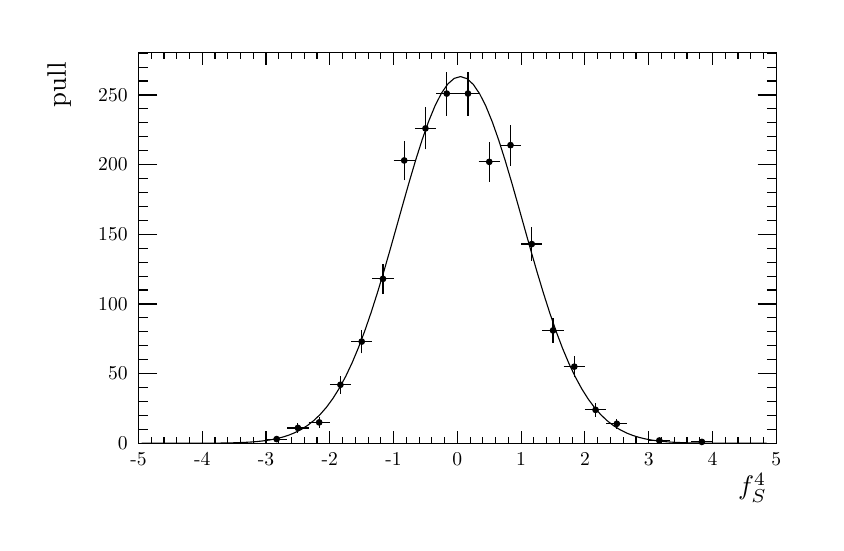
\begin{tikzpicture}
\pgfdeclareplotmark{cross} {
\pgfpathmoveto{\pgfpoint{-0.3\pgfplotmarksize}{\pgfplotmarksize}}
\pgfpathlineto{\pgfpoint{+0.3\pgfplotmarksize}{\pgfplotmarksize}}
\pgfpathlineto{\pgfpoint{+0.3\pgfplotmarksize}{0.3\pgfplotmarksize}}
\pgfpathlineto{\pgfpoint{+1\pgfplotmarksize}{0.3\pgfplotmarksize}}
\pgfpathlineto{\pgfpoint{+1\pgfplotmarksize}{-0.3\pgfplotmarksize}}
\pgfpathlineto{\pgfpoint{+0.3\pgfplotmarksize}{-0.3\pgfplotmarksize}}
\pgfpathlineto{\pgfpoint{+0.3\pgfplotmarksize}{-1.\pgfplotmarksize}}
\pgfpathlineto{\pgfpoint{-0.3\pgfplotmarksize}{-1.\pgfplotmarksize}}
\pgfpathlineto{\pgfpoint{-0.3\pgfplotmarksize}{-0.3\pgfplotmarksize}}
\pgfpathlineto{\pgfpoint{-1.\pgfplotmarksize}{-0.3\pgfplotmarksize}}
\pgfpathlineto{\pgfpoint{-1.\pgfplotmarksize}{0.3\pgfplotmarksize}}
\pgfpathlineto{\pgfpoint{-0.3\pgfplotmarksize}{0.3\pgfplotmarksize}}
\pgfpathclose
\pgfusepathqstroke
}
\pgfdeclareplotmark{cross*} {
\pgfpathmoveto{\pgfpoint{-0.3\pgfplotmarksize}{\pgfplotmarksize}}
\pgfpathlineto{\pgfpoint{+0.3\pgfplotmarksize}{\pgfplotmarksize}}
\pgfpathlineto{\pgfpoint{+0.3\pgfplotmarksize}{0.3\pgfplotmarksize}}
\pgfpathlineto{\pgfpoint{+1\pgfplotmarksize}{0.3\pgfplotmarksize}}
\pgfpathlineto{\pgfpoint{+1\pgfplotmarksize}{-0.3\pgfplotmarksize}}
\pgfpathlineto{\pgfpoint{+0.3\pgfplotmarksize}{-0.3\pgfplotmarksize}}
\pgfpathlineto{\pgfpoint{+0.3\pgfplotmarksize}{-1.\pgfplotmarksize}}
\pgfpathlineto{\pgfpoint{-0.3\pgfplotmarksize}{-1.\pgfplotmarksize}}
\pgfpathlineto{\pgfpoint{-0.3\pgfplotmarksize}{-0.3\pgfplotmarksize}}
\pgfpathlineto{\pgfpoint{-1.\pgfplotmarksize}{-0.3\pgfplotmarksize}}
\pgfpathlineto{\pgfpoint{-1.\pgfplotmarksize}{0.3\pgfplotmarksize}}
\pgfpathlineto{\pgfpoint{-0.3\pgfplotmarksize}{0.3\pgfplotmarksize}}
\pgfpathclose
\pgfusepathqfillstroke
}
\pgfdeclareplotmark{newstar} {
\pgfpathmoveto{\pgfqpoint{0pt}{\pgfplotmarksize}}
\pgfpathlineto{\pgfqpointpolar{44}{0.5\pgfplotmarksize}}
\pgfpathlineto{\pgfqpointpolar{18}{\pgfplotmarksize}}
\pgfpathlineto{\pgfqpointpolar{-20}{0.5\pgfplotmarksize}}
\pgfpathlineto{\pgfqpointpolar{-54}{\pgfplotmarksize}}
\pgfpathlineto{\pgfqpointpolar{-90}{0.5\pgfplotmarksize}}
\pgfpathlineto{\pgfqpointpolar{234}{\pgfplotmarksize}}
\pgfpathlineto{\pgfqpointpolar{198}{0.5\pgfplotmarksize}}
\pgfpathlineto{\pgfqpointpolar{162}{\pgfplotmarksize}}
\pgfpathlineto{\pgfqpointpolar{134}{0.5\pgfplotmarksize}}
\pgfpathclose
\pgfusepathqstroke
}
\pgfdeclareplotmark{newstar*} {
\pgfpathmoveto{\pgfqpoint{0pt}{\pgfplotmarksize}}
\pgfpathlineto{\pgfqpointpolar{44}{0.5\pgfplotmarksize}}
\pgfpathlineto{\pgfqpointpolar{18}{\pgfplotmarksize}}
\pgfpathlineto{\pgfqpointpolar{-20}{0.5\pgfplotmarksize}}
\pgfpathlineto{\pgfqpointpolar{-54}{\pgfplotmarksize}}
\pgfpathlineto{\pgfqpointpolar{-90}{0.5\pgfplotmarksize}}
\pgfpathlineto{\pgfqpointpolar{234}{\pgfplotmarksize}}
\pgfpathlineto{\pgfqpointpolar{198}{0.5\pgfplotmarksize}}
\pgfpathlineto{\pgfqpointpolar{162}{\pgfplotmarksize}}
\pgfpathlineto{\pgfqpointpolar{134}{0.5\pgfplotmarksize}}
\pgfpathclose
\pgfusepathqfillstroke
}
\definecolor{c}{rgb}{1,1,1};
\draw [color=c, fill=c] (0,0) rectangle (10,6.27517);
\draw [color=c, fill=c] (1.4,1.00403) rectangle (9.5,5.96141);
\definecolor{c}{rgb}{0,0,0};
\draw [c] (1.4,1.00403) -- (1.4,5.96141) -- (9.5,5.96141) -- (9.5,1.00403) -- (1.4,1.00403);
\draw [c] (3.155,1.02646) -- (3.155,1.05711);
\draw [c] (3.155,1.05711) -- (3.155,1.08775);
\draw [c] (3.02,1.05711) -- (3.155,1.05711);
\draw [c] (3.155,1.05711) -- (3.29,1.05711);
\foreach \P in {(3.155,1.05711)}{\draw[mark options={color=c,fill=c},mark size=2.402402pt,mark=*,mark size=1pt] plot coordinates {\P};}
\draw [c] (3.425,1.13997) -- (3.425,1.19865);
\draw [c] (3.425,1.19865) -- (3.425,1.25733);
\draw [c] (3.29,1.19865) -- (3.425,1.19865);
\draw [c] (3.425,1.19865) -- (3.56,1.19865);
\foreach \P in {(3.425,1.19865)}{\draw[mark options={color=c,fill=c},mark size=2.402402pt,mark=*,mark size=1pt] plot coordinates {\P};}
\draw [c] (3.695,1.2009) -- (3.695,1.26943);
\draw [c] (3.695,1.26943) -- (3.695,1.33795);
\draw [c] (3.56,1.26943) -- (3.695,1.26943);
\draw [c] (3.695,1.26943) -- (3.83,1.26943);
\foreach \P in {(3.695,1.26943)}{\draw[mark options={color=c,fill=c},mark size=2.402402pt,mark=*,mark size=1pt] plot coordinates {\P};}
\draw [c] (3.965,1.63248) -- (3.965,1.74714);
\draw [c] (3.965,1.74714) -- (3.965,1.86181);
\draw [c] (3.83,1.74714) -- (3.965,1.74714);
\draw [c] (3.965,1.74714) -- (4.1,1.74714);
\foreach \P in {(3.965,1.74714)}{\draw[mark options={color=c,fill=c},mark size=2.402402pt,mark=*,mark size=1pt] plot coordinates {\P};}
\draw [c] (4.235,2.14446) -- (4.235,2.29563);
\draw [c] (4.235,2.29563) -- (4.235,2.4468);
\draw [c] (4.1,2.29563) -- (4.235,2.29563);
\draw [c] (4.235,2.29563) -- (4.37,2.29563);
\foreach \P in {(4.235,2.29563)}{\draw[mark options={color=c,fill=c},mark size=2.402402pt,mark=*,mark size=1pt] plot coordinates {\P};}
\draw [c] (4.505,2.89963) -- (4.505,3.09183);
\draw [c] (4.505,3.09183) -- (4.505,3.28403);
\draw [c] (4.37,3.09183) -- (4.505,3.09183);
\draw [c] (4.505,3.09183) -- (4.64,3.09183);
\foreach \P in {(4.505,3.09183)}{\draw[mark options={color=c,fill=c},mark size=2.402402pt,mark=*,mark size=1pt] plot coordinates {\P};}
\draw [c] (4.775,4.34366) -- (4.775,4.59575);
\draw [c] (4.775,4.59575) -- (4.775,4.84784);
\draw [c] (4.64,4.59575) -- (4.775,4.59575);
\draw [c] (4.775,4.59575) -- (4.91,4.59575);
\foreach \P in {(4.775,4.59575)}{\draw[mark options={color=c,fill=c},mark size=2.402402pt,mark=*,mark size=1pt] plot coordinates {\P};}
\draw [c] (5.045,4.73671) -- (5.045,5.0027);
\draw [c] (5.045,5.0027) -- (5.045,5.26869);
\draw [c] (4.91,5.0027) -- (5.045,5.0027);
\draw [c] (5.045,5.0027) -- (5.18,5.0027);
\foreach \P in {(5.045,5.0027)}{\draw[mark options={color=c,fill=c},mark size=2.402402pt,mark=*,mark size=1pt] plot coordinates {\P};}
\draw [c] (5.315,5.16472) -- (5.315,5.44503);
\draw [c] (5.315,5.44503) -- (5.315,5.72534);
\draw [c] (5.18,5.44503) -- (5.315,5.44503);
\draw [c] (5.315,5.44503) -- (5.45,5.44503);
\foreach \P in {(5.315,5.44503)}{\draw[mark options={color=c,fill=c},mark size=2.402402pt,mark=*,mark size=1pt] plot coordinates {\P};}
\draw [c] (5.585,5.16472) -- (5.585,5.44503);
\draw [c] (5.585,5.44503) -- (5.585,5.72534);
\draw [c] (5.45,5.44503) -- (5.585,5.44503);
\draw [c] (5.585,5.44503) -- (5.72,5.44503);
\foreach \P in {(5.585,5.44503)}{\draw[mark options={color=c,fill=c},mark size=2.402402pt,mark=*,mark size=1pt] plot coordinates {\P};}
\draw [c] (5.855,4.32659) -- (5.855,4.57806);
\draw [c] (5.855,4.57806) -- (5.855,4.82953);
\draw [c] (5.72,4.57806) -- (5.855,4.57806);
\draw [c] (5.855,4.57806) -- (5.99,4.57806);
\foreach \P in {(5.855,4.57806)}{\draw[mark options={color=c,fill=c},mark size=2.402402pt,mark=*,mark size=1pt] plot coordinates {\P};}
\draw [c] (6.125,4.53155) -- (6.125,4.79038);
\draw [c] (6.125,4.79038) -- (6.125,5.04921);
\draw [c] (5.99,4.79038) -- (6.125,4.79038);
\draw [c] (6.125,4.79038) -- (6.26,4.79038);
\foreach \P in {(6.125,4.79038)}{\draw[mark options={color=c,fill=c},mark size=2.402402pt,mark=*,mark size=1pt] plot coordinates {\P};}
\draw [c] (6.395,3.32258) -- (6.395,3.53416);
\draw [c] (6.395,3.53416) -- (6.395,3.74574);
\draw [c] (6.26,3.53416) -- (6.395,3.53416);
\draw [c] (6.395,3.53416) -- (6.53,3.53416);
\foreach \P in {(6.395,3.53416)}{\draw[mark options={color=c,fill=c},mark size=2.402402pt,mark=*,mark size=1pt] plot coordinates {\P};}
\draw [c] (6.665,2.27794) -- (6.665,2.43718);
\draw [c] (6.665,2.43718) -- (6.665,2.59642);
\draw [c] (6.53,2.43718) -- (6.665,2.43718);
\draw [c] (6.665,2.43718) -- (6.8,2.43718);
\foreach \P in {(6.665,2.43718)}{\draw[mark options={color=c,fill=c},mark size=2.402402pt,mark=*,mark size=1pt] plot coordinates {\P};}
\draw [c] (6.935,1.84594) -- (6.935,1.97715);
\draw [c] (6.935,1.97715) -- (6.935,2.10837);
\draw [c] (6.8,1.97715) -- (6.935,1.97715);
\draw [c] (6.935,1.97715) -- (7.07,1.97715);
\foreach \P in {(6.935,1.97715)}{\draw[mark options={color=c,fill=c},mark size=2.402402pt,mark=*,mark size=1pt] plot coordinates {\P};}
\draw [c] (7.205,1.34199) -- (7.205,1.42866);
\draw [c] (7.205,1.42866) -- (7.205,1.51534);
\draw [c] (7.07,1.42866) -- (7.205,1.42866);
\draw [c] (7.205,1.42866) -- (7.34,1.42866);
\foreach \P in {(7.205,1.42866)}{\draw[mark options={color=c,fill=c},mark size=2.402402pt,mark=*,mark size=1pt] plot coordinates {\P};}
\draw [c] (7.475,1.18553) -- (7.475,1.25173);
\draw [c] (7.475,1.25173) -- (7.475,1.31793);
\draw [c] (7.34,1.25173) -- (7.475,1.25173);
\draw [c] (7.475,1.25173) -- (7.61,1.25173);
\foreach \P in {(7.475,1.25173)}{\draw[mark options={color=c,fill=c},mark size=2.402402pt,mark=*,mark size=1pt] plot coordinates {\P};}
\draw [c] (8.015,1.01439) -- (8.015,1.03941);
\draw [c] (8.015,1.03941) -- (8.015,1.06444);
\draw [c] (7.88,1.03941) -- (8.015,1.03941);
\draw [c] (8.015,1.03941) -- (8.15,1.03941);
\foreach \P in {(8.015,1.03941)}{\draw[mark options={color=c,fill=c},mark size=2.402402pt,mark=*,mark size=1pt] plot coordinates {\P};}
\draw [c] (8.555,1.00403) -- (8.555,1.02172);
\draw [c] (8.555,1.02172) -- (8.555,1.03941);
\draw [c] (8.42,1.02172) -- (8.555,1.02172);
\draw [c] (8.555,1.02172) -- (8.69,1.02172);
\foreach \P in {(8.555,1.02172)}{\draw[mark options={color=c,fill=c},mark size=2.402402pt,mark=*,mark size=1pt] plot coordinates {\P};}
\draw [c,line width=0.4] (1.4405,1.00403) -- (1.5215,1.00403) -- (1.6025,1.00403) -- (1.6835,1.00403) -- (1.7645,1.00403) -- (1.8455,1.00403) -- (1.9265,1.00403) -- (2.0075,1.00403) -- (2.0885,1.00403) -- (2.1695,1.0047) -- (2.2505,1.00506) --
 (2.3315,1.0056) -- (2.4125,1.00638) -- (2.4935,1.00752) -- (2.5745,1.00916) -- (2.6555,1.01148) -- (2.7365,1.01474) -- (2.8175,1.01926) -- (2.8985,1.02547) -- (2.9795,1.03389) -- (3.0605,1.04519) -- (3.1415,1.06017) -- (3.2225,1.07979) --
 (3.3035,1.1052) -- (3.3845,1.13772) -- (3.4655,1.17884) -- (3.5465,1.23021) -- (3.6275,1.29361) -- (3.7085,1.3709) -- (3.7895,1.46396) -- (3.8705,1.57458) -- (3.9515,1.70439) -- (4.0325,1.85473) -- (4.1135,2.02652) -- (4.1945,2.22013) --
 (4.2755,2.43526) -- (4.3565,2.6708) -- (4.4375,2.92477) -- (4.5185,3.19426) -- (4.5995,3.47541) -- (4.6805,3.76344) -- (4.7615,4.05277) -- (4.8425,4.33716) -- (4.9235,4.60992) -- (5.0045,4.86414) -- (5.0855,5.09301) -- (5.1665,5.29008) --
 (5.2475,5.4496) -- (5.3285,5.56677) -- (5.4095,5.63797);
\draw [c,line width=0.4] (5.4095,5.63797) -- (5.4905,5.66101) -- (5.5715,5.63513) -- (5.6525,5.56118) -- (5.7335,5.44143) -- (5.8145,5.27958) -- (5.8955,5.08049) -- (5.9765,4.84997) -- (6.0575,4.59448) -- (6.1385,4.32086) -- (6.2195,4.036) --
 (6.3005,3.74658) -- (6.3815,3.4588) -- (6.4625,3.17821) -- (6.5435,2.90952) -- (6.6245,2.65655) -- (6.7055,2.42216) -- (6.7865,2.20826) -- (6.8675,2.01592) -- (6.9485,1.84539) -- (7.0295,1.69628) -- (7.1105,1.56762) -- (7.1915,1.45807) --
 (7.2725,1.36599) -- (7.3535,1.28956) -- (7.4345,1.2269) -- (7.5155,1.17618) -- (7.5965,1.1356) -- (7.6775,1.10354) -- (7.7585,1.0785) -- (7.8395,1.05918) -- (7.9205,1.04444) -- (8.0015,1.03333) -- (8.0825,1.02505) -- (8.1635,1.01896) --
 (8.2445,1.01452) -- (8.3255,1.01132) -- (8.4065,1.00904) -- (8.4875,1.00744) -- (8.5685,1.00633) -- (8.6495,1.00556) -- (8.7305,1.00504) -- (8.8115,1.00469) -- (8.8925,1.00403) -- (8.9735,1.00403) -- (9.0545,1.00403) -- (9.1355,1.00403) --
 (9.2165,1.00403) -- (9.2975,1.00403) -- (9.3785,1.00403);
\draw [c,line width=0.4] (9.3785,1.00403) -- (9.4595,1.00403);
\draw [c,line width=0.4] (1.4,1.00403) -- (9.5,1.00403);
\draw [anchor= east] (9.5,0.441772) node[scale=0.96888, rotate=0]{$f_\text{S}^4$};
\draw [c,line width=0.4] (1.4,1.15651) -- (1.4,1.00403);
\draw [c,line width=0.4] (1.562,1.08027) -- (1.562,1.00403);
\draw [c,line width=0.4] (1.724,1.08027) -- (1.724,1.00403);
\draw [c,line width=0.4] (1.886,1.08027) -- (1.886,1.00403);
\draw [c,line width=0.4] (2.048,1.08027) -- (2.048,1.00403);
\draw [c,line width=0.4] (2.21,1.15651) -- (2.21,1.00403);
\draw [c,line width=0.4] (2.372,1.08027) -- (2.372,1.00403);
\draw [c,line width=0.4] (2.534,1.08027) -- (2.534,1.00403);
\draw [c,line width=0.4] (2.696,1.08027) -- (2.696,1.00403);
\draw [c,line width=0.4] (2.858,1.08027) -- (2.858,1.00403);
\draw [c,line width=0.4] (3.02,1.15651) -- (3.02,1.00403);
\draw [c,line width=0.4] (3.182,1.08027) -- (3.182,1.00403);
\draw [c,line width=0.4] (3.344,1.08027) -- (3.344,1.00403);
\draw [c,line width=0.4] (3.506,1.08027) -- (3.506,1.00403);
\draw [c,line width=0.4] (3.668,1.08027) -- (3.668,1.00403);
\draw [c,line width=0.4] (3.83,1.15651) -- (3.83,1.00403);
\draw [c,line width=0.4] (3.992,1.08027) -- (3.992,1.00403);
\draw [c,line width=0.4] (4.154,1.08027) -- (4.154,1.00403);
\draw [c,line width=0.4] (4.316,1.08027) -- (4.316,1.00403);
\draw [c,line width=0.4] (4.478,1.08027) -- (4.478,1.00403);
\draw [c,line width=0.4] (4.64,1.15651) -- (4.64,1.00403);
\draw [c,line width=0.4] (4.802,1.08027) -- (4.802,1.00403);
\draw [c,line width=0.4] (4.964,1.08027) -- (4.964,1.00403);
\draw [c,line width=0.4] (5.126,1.08027) -- (5.126,1.00403);
\draw [c,line width=0.4] (5.288,1.08027) -- (5.288,1.00403);
\draw [c,line width=0.4] (5.45,1.15651) -- (5.45,1.00403);
\draw [c,line width=0.4] (5.612,1.08027) -- (5.612,1.00403);
\draw [c,line width=0.4] (5.774,1.08027) -- (5.774,1.00403);
\draw [c,line width=0.4] (5.936,1.08027) -- (5.936,1.00403);
\draw [c,line width=0.4] (6.098,1.08027) -- (6.098,1.00403);
\draw [c,line width=0.4] (6.26,1.15651) -- (6.26,1.00403);
\draw [c,line width=0.4] (6.422,1.08027) -- (6.422,1.00403);
\draw [c,line width=0.4] (6.584,1.08027) -- (6.584,1.00403);
\draw [c,line width=0.4] (6.746,1.08027) -- (6.746,1.00403);
\draw [c,line width=0.4] (6.908,1.08027) -- (6.908,1.00403);
\draw [c,line width=0.4] (7.07,1.15651) -- (7.07,1.00403);
\draw [c,line width=0.4] (7.232,1.08027) -- (7.232,1.00403);
\draw [c,line width=0.4] (7.394,1.08027) -- (7.394,1.00403);
\draw [c,line width=0.4] (7.556,1.08027) -- (7.556,1.00403);
\draw [c,line width=0.4] (7.718,1.08027) -- (7.718,1.00403);
\draw [c,line width=0.4] (7.88,1.15651) -- (7.88,1.00403);
\draw [c,line width=0.4] (8.042,1.08027) -- (8.042,1.00403);
\draw [c,line width=0.4] (8.204,1.08027) -- (8.204,1.00403);
\draw [c,line width=0.4] (8.366,1.08027) -- (8.366,1.00403);
\draw [c,line width=0.4] (8.528,1.08027) -- (8.528,1.00403);
\draw [c,line width=0.4] (8.69,1.15651) -- (8.69,1.00403);
\draw [c,line width=0.4] (8.852,1.08027) -- (8.852,1.00403);
\draw [c,line width=0.4] (9.014,1.08027) -- (9.014,1.00403);
\draw [c,line width=0.4] (9.176,1.08027) -- (9.176,1.00403);
\draw [c,line width=0.4] (9.338,1.08027) -- (9.338,1.00403);
\draw [c,line width=0.4] (9.5,1.15651) -- (9.5,1.00403);
\draw [anchor=base] (1.4,0.721644) node[scale=0.708027, rotate=0]{-5};
\draw [anchor=base] (2.21,0.721644) node[scale=0.708027, rotate=0]{-4};
\draw [anchor=base] (3.02,0.721644) node[scale=0.708027, rotate=0]{-3};
\draw [anchor=base] (3.83,0.721644) node[scale=0.708027, rotate=0]{-2};
\draw [anchor=base] (4.64,0.721644) node[scale=0.708027, rotate=0]{-1};
\draw [anchor=base] (5.45,0.721644) node[scale=0.708027, rotate=0]{0};
\draw [anchor=base] (6.26,0.721644) node[scale=0.708027, rotate=0]{1};
\draw [anchor=base] (7.07,0.721644) node[scale=0.708027, rotate=0]{2};
\draw [anchor=base] (7.88,0.721644) node[scale=0.708027, rotate=0]{3};
\draw [anchor=base] (8.69,0.721644) node[scale=0.708027, rotate=0]{4};
\draw [anchor=base] (9.5,0.721644) node[scale=0.708027, rotate=0]{5};
\draw [c,line width=0.4] (1.4,5.96141) -- (9.5,5.96141);
\draw [c,line width=0.4] (1.4,5.80892) -- (1.4,5.96141);
\draw [c,line width=0.4] (1.562,5.88517) -- (1.562,5.96141);
\draw [c,line width=0.4] (1.724,5.88517) -- (1.724,5.96141);
\draw [c,line width=0.4] (1.886,5.88517) -- (1.886,5.96141);
\draw [c,line width=0.4] (2.048,5.88517) -- (2.048,5.96141);
\draw [c,line width=0.4] (2.21,5.80892) -- (2.21,5.96141);
\draw [c,line width=0.4] (2.372,5.88517) -- (2.372,5.96141);
\draw [c,line width=0.4] (2.534,5.88517) -- (2.534,5.96141);
\draw [c,line width=0.4] (2.696,5.88517) -- (2.696,5.96141);
\draw [c,line width=0.4] (2.858,5.88517) -- (2.858,5.96141);
\draw [c,line width=0.4] (3.02,5.80892) -- (3.02,5.96141);
\draw [c,line width=0.4] (3.182,5.88517) -- (3.182,5.96141);
\draw [c,line width=0.4] (3.344,5.88517) -- (3.344,5.96141);
\draw [c,line width=0.4] (3.506,5.88517) -- (3.506,5.96141);
\draw [c,line width=0.4] (3.668,5.88517) -- (3.668,5.96141);
\draw [c,line width=0.4] (3.83,5.80892) -- (3.83,5.96141);
\draw [c,line width=0.4] (3.992,5.88517) -- (3.992,5.96141);
\draw [c,line width=0.4] (4.154,5.88517) -- (4.154,5.96141);
\draw [c,line width=0.4] (4.316,5.88517) -- (4.316,5.96141);
\draw [c,line width=0.4] (4.478,5.88517) -- (4.478,5.96141);
\draw [c,line width=0.4] (4.64,5.80892) -- (4.64,5.96141);
\draw [c,line width=0.4] (4.802,5.88517) -- (4.802,5.96141);
\draw [c,line width=0.4] (4.964,5.88517) -- (4.964,5.96141);
\draw [c,line width=0.4] (5.126,5.88517) -- (5.126,5.96141);
\draw [c,line width=0.4] (5.288,5.88517) -- (5.288,5.96141);
\draw [c,line width=0.4] (5.45,5.80892) -- (5.45,5.96141);
\draw [c,line width=0.4] (5.612,5.88517) -- (5.612,5.96141);
\draw [c,line width=0.4] (5.774,5.88517) -- (5.774,5.96141);
\draw [c,line width=0.4] (5.936,5.88517) -- (5.936,5.96141);
\draw [c,line width=0.4] (6.098,5.88517) -- (6.098,5.96141);
\draw [c,line width=0.4] (6.26,5.80892) -- (6.26,5.96141);
\draw [c,line width=0.4] (6.422,5.88517) -- (6.422,5.96141);
\draw [c,line width=0.4] (6.584,5.88517) -- (6.584,5.96141);
\draw [c,line width=0.4] (6.746,5.88517) -- (6.746,5.96141);
\draw [c,line width=0.4] (6.908,5.88517) -- (6.908,5.96141);
\draw [c,line width=0.4] (7.07,5.80892) -- (7.07,5.96141);
\draw [c,line width=0.4] (7.232,5.88517) -- (7.232,5.96141);
\draw [c,line width=0.4] (7.394,5.88517) -- (7.394,5.96141);
\draw [c,line width=0.4] (7.556,5.88517) -- (7.556,5.96141);
\draw [c,line width=0.4] (7.718,5.88517) -- (7.718,5.96141);
\draw [c,line width=0.4] (7.88,5.80892) -- (7.88,5.96141);
\draw [c,line width=0.4] (8.042,5.88517) -- (8.042,5.96141);
\draw [c,line width=0.4] (8.204,5.88517) -- (8.204,5.96141);
\draw [c,line width=0.4] (8.366,5.88517) -- (8.366,5.96141);
\draw [c,line width=0.4] (8.528,5.88517) -- (8.528,5.96141);
\draw [c,line width=0.4] (8.69,5.80892) -- (8.69,5.96141);
\draw [c,line width=0.4] (8.852,5.88517) -- (8.852,5.96141);
\draw [c,line width=0.4] (9.014,5.88517) -- (9.014,5.96141);
\draw [c,line width=0.4] (9.176,5.88517) -- (9.176,5.96141);
\draw [c,line width=0.4] (9.338,5.88517) -- (9.338,5.96141);
\draw [c,line width=0.4] (9.5,5.80892) -- (9.5,5.96141);
\draw [c,line width=0.4] (1.4,1.00403) -- (1.4,5.96141);
\draw [anchor= east] (0.392,5.96141) node[scale=0.96888, rotate=90]{pull};
\draw [c,line width=0.4] (1.637,1.00403) -- (1.4,1.00403);
\draw [c,line width=0.4] (1.5185,1.18096) -- (1.4,1.18096);
\draw [c,line width=0.4] (1.5185,1.35789) -- (1.4,1.35789);
\draw [c,line width=0.4] (1.5185,1.53482) -- (1.4,1.53482);
\draw [c,line width=0.4] (1.5185,1.71176) -- (1.4,1.71176);
\draw [c,line width=0.4] (1.637,1.88869) -- (1.4,1.88869);
\draw [c,line width=0.4] (1.5185,2.06562) -- (1.4,2.06562);
\draw [c,line width=0.4] (1.5185,2.24255) -- (1.4,2.24255);
\draw [c,line width=0.4] (1.5185,2.41949) -- (1.4,2.41949);
\draw [c,line width=0.4] (1.5185,2.59642) -- (1.4,2.59642);
\draw [c,line width=0.4] (1.637,2.77335) -- (1.4,2.77335);
\draw [c,line width=0.4] (1.5185,2.95028) -- (1.4,2.95028);
\draw [c,line width=0.4] (1.5185,3.12722) -- (1.4,3.12722);
\draw [c,line width=0.4] (1.5185,3.30415) -- (1.4,3.30415);
\draw [c,line width=0.4] (1.5185,3.48108) -- (1.4,3.48108);
\draw [c,line width=0.4] (1.637,3.65801) -- (1.4,3.65801);
\draw [c,line width=0.4] (1.5185,3.83495) -- (1.4,3.83495);
\draw [c,line width=0.4] (1.5185,4.01188) -- (1.4,4.01188);
\draw [c,line width=0.4] (1.5185,4.18881) -- (1.4,4.18881);
\draw [c,line width=0.4] (1.5185,4.36574) -- (1.4,4.36574);
\draw [c,line width=0.4] (1.637,4.54268) -- (1.4,4.54268);
\draw [c,line width=0.4] (1.5185,4.71961) -- (1.4,4.71961);
\draw [c,line width=0.4] (1.5185,4.89654) -- (1.4,4.89654);
\draw [c,line width=0.4] (1.5185,5.07347) -- (1.4,5.07347);
\draw [c,line width=0.4] (1.5185,5.2504) -- (1.4,5.2504);
\draw [c,line width=0.4] (1.637,5.42734) -- (1.4,5.42734);
\draw [c,line width=0.4] (1.637,5.42734) -- (1.4,5.42734);
\draw [c,line width=0.4] (1.5185,5.60427) -- (1.4,5.60427);
\draw [c,line width=0.4] (1.5185,5.7812) -- (1.4,5.7812);
\draw [c,line width=0.4] (1.5185,5.95813) -- (1.4,5.95813);
\draw [anchor= east] (1.35,1.00403) node[scale=0.708027, rotate=0]{0};
\draw [anchor= east] (1.35,1.88869) node[scale=0.708027, rotate=0]{50};
\draw [anchor= east] (1.35,2.77335) node[scale=0.708027, rotate=0]{100};
\draw [anchor= east] (1.35,3.65801) node[scale=0.708027, rotate=0]{150};
\draw [anchor= east] (1.35,4.54268) node[scale=0.708027, rotate=0]{200};
\draw [anchor= east] (1.35,5.42734) node[scale=0.708027, rotate=0]{250};
\draw [c,line width=0.4] (9.5,1.00403) -- (9.5,5.96141);
\draw [c,line width=0.4] (9.263,1.00403) -- (9.5,1.00403);
\draw [c,line width=0.4] (9.3815,1.18096) -- (9.5,1.18096);
\draw [c,line width=0.4] (9.3815,1.35789) -- (9.5,1.35789);
\draw [c,line width=0.4] (9.3815,1.53482) -- (9.5,1.53482);
\draw [c,line width=0.4] (9.3815,1.71176) -- (9.5,1.71176);
\draw [c,line width=0.4] (9.263,1.88869) -- (9.5,1.88869);
\draw [c,line width=0.4] (9.3815,2.06562) -- (9.5,2.06562);
\draw [c,line width=0.4] (9.3815,2.24255) -- (9.5,2.24255);
\draw [c,line width=0.4] (9.3815,2.41949) -- (9.5,2.41949);
\draw [c,line width=0.4] (9.3815,2.59642) -- (9.5,2.59642);
\draw [c,line width=0.4] (9.263,2.77335) -- (9.5,2.77335);
\draw [c,line width=0.4] (9.3815,2.95028) -- (9.5,2.95028);
\draw [c,line width=0.4] (9.3815,3.12722) -- (9.5,3.12722);
\draw [c,line width=0.4] (9.3815,3.30415) -- (9.5,3.30415);
\draw [c,line width=0.4] (9.3815,3.48108) -- (9.5,3.48108);
\draw [c,line width=0.4] (9.263,3.65801) -- (9.5,3.65801);
\draw [c,line width=0.4] (9.3815,3.83495) -- (9.5,3.83495);
\draw [c,line width=0.4] (9.3815,4.01188) -- (9.5,4.01188);
\draw [c,line width=0.4] (9.3815,4.18881) -- (9.5,4.18881);
\draw [c,line width=0.4] (9.3815,4.36574) -- (9.5,4.36574);
\draw [c,line width=0.4] (9.263,4.54268) -- (9.5,4.54268);
\draw [c,line width=0.4] (9.3815,4.71961) -- (9.5,4.71961);
\draw [c,line width=0.4] (9.3815,4.89654) -- (9.5,4.89654);
\draw [c,line width=0.4] (9.3815,5.07347) -- (9.5,5.07347);
\draw [c,line width=0.4] (9.3815,5.2504) -- (9.5,5.2504);
\draw [c,line width=0.4] (9.263,5.42734) -- (9.5,5.42734);
\draw [c,line width=0.4] (9.263,5.42734) -- (9.5,5.42734);
\draw [c,line width=0.4] (9.3815,5.60427) -- (9.5,5.60427);
\draw [c,line width=0.4] (9.3815,5.7812) -- (9.5,5.7812);
\draw [c,line width=0.4] (9.3815,5.95813) -- (9.5,5.95813);
\end{tikzpicture}
}
    \caption{}
    \label{pull_ASMag2_bin4}
  \end{subfigure}%
  \hfill%
  \begin{subfigure}{0.5\textwidth}
    \tikzsetnextfilename{pull_ASPhase_bin4} 
    \scalebox{0.60}{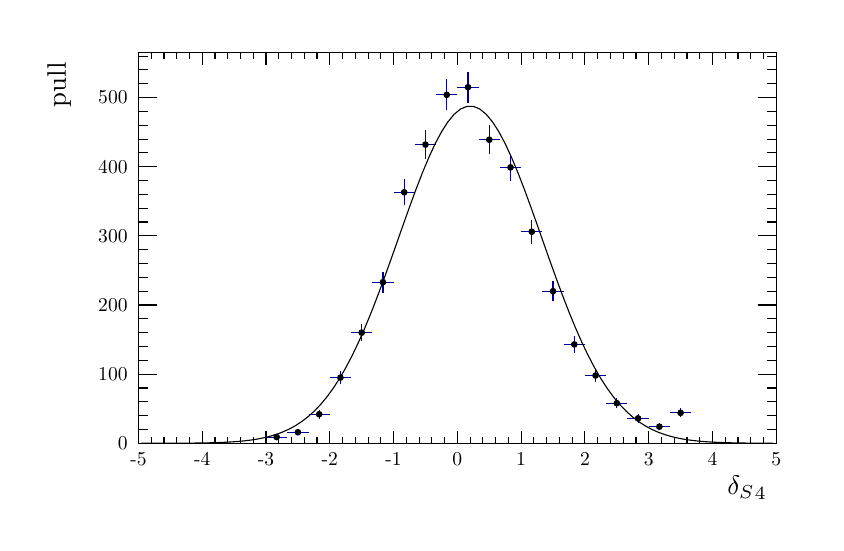
\begin{tikzpicture}
\pgfdeclareplotmark{cross} {
\pgfpathmoveto{\pgfpoint{-0.3\pgfplotmarksize}{\pgfplotmarksize}}
\pgfpathlineto{\pgfpoint{+0.3\pgfplotmarksize}{\pgfplotmarksize}}
\pgfpathlineto{\pgfpoint{+0.3\pgfplotmarksize}{0.3\pgfplotmarksize}}
\pgfpathlineto{\pgfpoint{+1\pgfplotmarksize}{0.3\pgfplotmarksize}}
\pgfpathlineto{\pgfpoint{+1\pgfplotmarksize}{-0.3\pgfplotmarksize}}
\pgfpathlineto{\pgfpoint{+0.3\pgfplotmarksize}{-0.3\pgfplotmarksize}}
\pgfpathlineto{\pgfpoint{+0.3\pgfplotmarksize}{-1.\pgfplotmarksize}}
\pgfpathlineto{\pgfpoint{-0.3\pgfplotmarksize}{-1.\pgfplotmarksize}}
\pgfpathlineto{\pgfpoint{-0.3\pgfplotmarksize}{-0.3\pgfplotmarksize}}
\pgfpathlineto{\pgfpoint{-1.\pgfplotmarksize}{-0.3\pgfplotmarksize}}
\pgfpathlineto{\pgfpoint{-1.\pgfplotmarksize}{0.3\pgfplotmarksize}}
\pgfpathlineto{\pgfpoint{-0.3\pgfplotmarksize}{0.3\pgfplotmarksize}}
\pgfpathclose
\pgfusepathqstroke
}
\pgfdeclareplotmark{cross*} {
\pgfpathmoveto{\pgfpoint{-0.3\pgfplotmarksize}{\pgfplotmarksize}}
\pgfpathlineto{\pgfpoint{+0.3\pgfplotmarksize}{\pgfplotmarksize}}
\pgfpathlineto{\pgfpoint{+0.3\pgfplotmarksize}{0.3\pgfplotmarksize}}
\pgfpathlineto{\pgfpoint{+1\pgfplotmarksize}{0.3\pgfplotmarksize}}
\pgfpathlineto{\pgfpoint{+1\pgfplotmarksize}{-0.3\pgfplotmarksize}}
\pgfpathlineto{\pgfpoint{+0.3\pgfplotmarksize}{-0.3\pgfplotmarksize}}
\pgfpathlineto{\pgfpoint{+0.3\pgfplotmarksize}{-1.\pgfplotmarksize}}
\pgfpathlineto{\pgfpoint{-0.3\pgfplotmarksize}{-1.\pgfplotmarksize}}
\pgfpathlineto{\pgfpoint{-0.3\pgfplotmarksize}{-0.3\pgfplotmarksize}}
\pgfpathlineto{\pgfpoint{-1.\pgfplotmarksize}{-0.3\pgfplotmarksize}}
\pgfpathlineto{\pgfpoint{-1.\pgfplotmarksize}{0.3\pgfplotmarksize}}
\pgfpathlineto{\pgfpoint{-0.3\pgfplotmarksize}{0.3\pgfplotmarksize}}
\pgfpathclose
\pgfusepathqfillstroke
}
\pgfdeclareplotmark{newstar} {
\pgfpathmoveto{\pgfqpoint{0pt}{\pgfplotmarksize}}
\pgfpathlineto{\pgfqpointpolar{44}{0.5\pgfplotmarksize}}
\pgfpathlineto{\pgfqpointpolar{18}{\pgfplotmarksize}}
\pgfpathlineto{\pgfqpointpolar{-20}{0.5\pgfplotmarksize}}
\pgfpathlineto{\pgfqpointpolar{-54}{\pgfplotmarksize}}
\pgfpathlineto{\pgfqpointpolar{-90}{0.5\pgfplotmarksize}}
\pgfpathlineto{\pgfqpointpolar{234}{\pgfplotmarksize}}
\pgfpathlineto{\pgfqpointpolar{198}{0.5\pgfplotmarksize}}
\pgfpathlineto{\pgfqpointpolar{162}{\pgfplotmarksize}}
\pgfpathlineto{\pgfqpointpolar{134}{0.5\pgfplotmarksize}}
\pgfpathclose
\pgfusepathqstroke
}
\pgfdeclareplotmark{newstar*} {
\pgfpathmoveto{\pgfqpoint{0pt}{\pgfplotmarksize}}
\pgfpathlineto{\pgfqpointpolar{44}{0.5\pgfplotmarksize}}
\pgfpathlineto{\pgfqpointpolar{18}{\pgfplotmarksize}}
\pgfpathlineto{\pgfqpointpolar{-20}{0.5\pgfplotmarksize}}
\pgfpathlineto{\pgfqpointpolar{-54}{\pgfplotmarksize}}
\pgfpathlineto{\pgfqpointpolar{-90}{0.5\pgfplotmarksize}}
\pgfpathlineto{\pgfqpointpolar{234}{\pgfplotmarksize}}
\pgfpathlineto{\pgfqpointpolar{198}{0.5\pgfplotmarksize}}
\pgfpathlineto{\pgfqpointpolar{162}{\pgfplotmarksize}}
\pgfpathlineto{\pgfqpointpolar{134}{0.5\pgfplotmarksize}}
\pgfpathclose
\pgfusepathqfillstroke
}
\definecolor{c}{rgb}{1,1,1};
\draw [color=c, fill=c] (0,0) rectangle (10,6.27517);
\draw [color=c, fill=c] (1.4,1.00403) rectangle (9.5,5.96141);
\definecolor{c}{rgb}{0,0,0};
\draw [c] (1.4,1.00403) -- (1.4,5.96141) -- (9.5,5.96141) -- (9.5,1.00403) -- (1.4,1.00403);
\definecolor{c}{rgb}{0,0,0.6};
\draw [c] (3.155,1.05671) -- (3.155,1.08305);
\draw [c] (3.155,1.08305) -- (3.155,1.1094);
\draw [c] (3.02,1.08305) -- (3.155,1.08305);
\draw [c] (3.155,1.08305) -- (3.29,1.08305);
\definecolor{c}{rgb}{0,0,0};
\foreach \P in {(3.155,1.08305)}{\draw[mark options={color=c,fill=c},mark size=2.402402pt,mark=*,mark size=1pt] plot coordinates {\P};}
\definecolor{c}{rgb}{0,0,0.6};
\draw [c] (3.425,1.1094) -- (3.425,1.14452);
\draw [c] (3.425,1.14452) -- (3.425,1.17964);
\draw [c] (3.29,1.14452) -- (3.425,1.14452);
\draw [c] (3.425,1.14452) -- (3.56,1.14452);
\definecolor{c}{rgb}{0,0,0};
\foreach \P in {(3.425,1.14452)}{\draw[mark options={color=c,fill=c},mark size=2.402402pt,mark=*,mark size=1pt] plot coordinates {\P};}
\definecolor{c}{rgb}{0,0,0.6};
\draw [c] (3.695,1.31591) -- (3.695,1.37282);
\draw [c] (3.695,1.37282) -- (3.695,1.42972);
\draw [c] (3.56,1.37282) -- (3.695,1.37282);
\draw [c] (3.695,1.37282) -- (3.83,1.37282);
\definecolor{c}{rgb}{0,0,0};
\foreach \P in {(3.695,1.37282)}{\draw[mark options={color=c,fill=c},mark size=2.402402pt,mark=*,mark size=1pt] plot coordinates {\P};}
\definecolor{c}{rgb}{0,0,0.6};
\draw [c] (3.965,1.75261) -- (3.965,1.83819);
\draw [c] (3.965,1.83819) -- (3.965,1.92378);
\draw [c] (3.83,1.83819) -- (3.965,1.83819);
\draw [c] (3.965,1.83819) -- (4.1,1.83819);
\definecolor{c}{rgb}{0,0,0};
\foreach \P in {(3.965,1.83819)}{\draw[mark options={color=c,fill=c},mark size=2.402402pt,mark=*,mark size=1pt] plot coordinates {\P};}
\definecolor{c}{rgb}{0,0,0.6};
\draw [c] (4.235,2.29787) -- (4.235,2.40894);
\draw [c] (4.235,2.40894) -- (4.235,2.52);
\draw [c] (4.1,2.40894) -- (4.235,2.40894);
\draw [c] (4.235,2.40894) -- (4.37,2.40894);
\definecolor{c}{rgb}{0,0,0};
\foreach \P in {(4.235,2.40894)}{\draw[mark options={color=c,fill=c},mark size=2.402402pt,mark=*,mark size=1pt] plot coordinates {\P};}
\definecolor{c}{rgb}{0,0,0.6};
\draw [c] (4.505,2.91589) -- (4.505,3.04993);
\draw [c] (4.505,3.04993) -- (4.505,3.18396);
\draw [c] (4.37,3.04993) -- (4.505,3.04993);
\draw [c] (4.505,3.04993) -- (4.64,3.04993);
\definecolor{c}{rgb}{0,0,0};
\foreach \P in {(4.505,3.04993)}{\draw[mark options={color=c,fill=c},mark size=2.402402pt,mark=*,mark size=1pt] plot coordinates {\P};}
\definecolor{c}{rgb}{0,0,0.6};
\draw [c] (4.775,4.02412) -- (4.775,4.19141);
\draw [c] (4.775,4.19141) -- (4.775,4.35871);
\draw [c] (4.64,4.19141) -- (4.775,4.19141);
\draw [c] (4.775,4.19141) -- (4.91,4.19141);
\definecolor{c}{rgb}{0,0,0};
\foreach \P in {(4.775,4.19141)}{\draw[mark options={color=c,fill=c},mark size=2.402402pt,mark=*,mark size=1pt] plot coordinates {\P};}
\definecolor{c}{rgb}{0,0,0.6};
\draw [c] (5.045,4.61478) -- (5.045,4.79728);
\draw [c] (5.045,4.79728) -- (5.045,4.97978);
\draw [c] (4.91,4.79728) -- (5.045,4.79728);
\draw [c] (5.045,4.79728) -- (5.18,4.79728);
\definecolor{c}{rgb}{0,0,0};
\foreach \P in {(5.045,4.79728)}{\draw[mark options={color=c,fill=c},mark size=2.402402pt,mark=*,mark size=1pt] plot coordinates {\P};}
\definecolor{c}{rgb}{0,0,0.6};
\draw [c] (5.315,5.23237) -- (5.315,5.42949);
\draw [c] (5.315,5.42949) -- (5.315,5.62662);
\draw [c] (5.18,5.42949) -- (5.315,5.42949);
\draw [c] (5.315,5.42949) -- (5.45,5.42949);
\definecolor{c}{rgb}{0,0,0};
\foreach \P in {(5.315,5.42949)}{\draw[mark options={color=c,fill=c},mark size=2.402402pt,mark=*,mark size=1pt] plot coordinates {\P};}
\definecolor{c}{rgb}{0,0,0.6};
\draw [c] (5.585,5.32681) -- (5.585,5.52608);
\draw [c] (5.585,5.52608) -- (5.585,5.72534);
\draw [c] (5.45,5.52608) -- (5.585,5.52608);
\draw [c] (5.585,5.52608) -- (5.72,5.52608);
\definecolor{c}{rgb}{0,0,0};
\foreach \P in {(5.585,5.52608)}{\draw[mark options={color=c,fill=c},mark size=2.402402pt,mark=*,mark size=1pt] plot coordinates {\P};}
\definecolor{c}{rgb}{0,0,0.6};
\draw [c] (5.855,4.67477) -- (5.855,4.85875);
\draw [c] (5.855,4.85875) -- (5.855,5.04272);
\draw [c] (5.72,4.85875) -- (5.855,4.85875);
\draw [c] (5.855,4.85875) -- (5.99,4.85875);
\definecolor{c}{rgb}{0,0,0};
\foreach \P in {(5.855,4.85875)}{\draw[mark options={color=c,fill=c},mark size=2.402402pt,mark=*,mark size=1pt] plot coordinates {\P};}
\definecolor{c}{rgb}{0,0,0.6};
\draw [c] (6.125,4.33213) -- (6.125,4.50752);
\draw [c] (6.125,4.50752) -- (6.125,4.68291);
\draw [c] (5.99,4.50752) -- (6.125,4.50752);
\draw [c] (6.125,4.50752) -- (6.26,4.50752);
\definecolor{c}{rgb}{0,0,0};
\foreach \P in {(6.125,4.50752)}{\draw[mark options={color=c,fill=c},mark size=2.402402pt,mark=*,mark size=1pt] plot coordinates {\P};}
\definecolor{c}{rgb}{0,0,0.6};
\draw [c] (6.395,3.53732) -- (6.395,3.69092);
\draw [c] (6.395,3.69092) -- (6.395,3.84451);
\draw [c] (6.26,3.69092) -- (6.395,3.69092);
\draw [c] (6.395,3.69092) -- (6.53,3.69092);
\definecolor{c}{rgb}{0,0,0};
\foreach \P in {(6.395,3.69092)}{\draw[mark options={color=c,fill=c},mark size=2.402402pt,mark=*,mark size=1pt] plot coordinates {\P};}
\definecolor{c}{rgb}{0,0,0.6};
\draw [c] (6.665,2.80554) -- (6.665,2.93578);
\draw [c] (6.665,2.93578) -- (6.665,3.06602);
\draw [c] (6.53,2.93578) -- (6.665,2.93578);
\draw [c] (6.665,2.93578) -- (6.8,2.93578);
\definecolor{c}{rgb}{0,0,0};
\foreach \P in {(6.665,2.93578)}{\draw[mark options={color=c,fill=c},mark size=2.402402pt,mark=*,mark size=1pt] plot coordinates {\P};}
\definecolor{c}{rgb}{0,0,0.6};
\draw [c] (6.935,2.15466) -- (6.935,2.25966);
\draw [c] (6.935,2.25966) -- (6.935,2.36467);
\draw [c] (6.8,2.25966) -- (6.935,2.25966);
\draw [c] (6.935,2.25966) -- (7.07,2.25966);
\definecolor{c}{rgb}{0,0,0};
\foreach \P in {(6.935,2.25966)}{\draw[mark options={color=c,fill=c},mark size=2.402402pt,mark=*,mark size=1pt] plot coordinates {\P};}
\definecolor{c}{rgb}{0,0,0.6};
\draw [c] (7.205,1.77761) -- (7.205,1.86453);
\draw [c] (7.205,1.86453) -- (7.205,1.95146);
\draw [c] (7.07,1.86453) -- (7.205,1.86453);
\draw [c] (7.205,1.86453) -- (7.34,1.86453);
\definecolor{c}{rgb}{0,0,0};
\foreach \P in {(7.205,1.86453)}{\draw[mark options={color=c,fill=c},mark size=2.402402pt,mark=*,mark size=1pt] plot coordinates {\P};}
\definecolor{c}{rgb}{0,0,0.6};
\draw [c] (7.475,1.44643) -- (7.475,1.51331);
\draw [c] (7.475,1.51331) -- (7.475,1.58018);
\draw [c] (7.34,1.51331) -- (7.475,1.51331);
\draw [c] (7.475,1.51331) -- (7.61,1.51331);
\definecolor{c}{rgb}{0,0,0};
\foreach \P in {(7.475,1.51331)}{\draw[mark options={color=c,fill=c},mark size=2.402402pt,mark=*,mark size=1pt] plot coordinates {\P};}
\definecolor{c}{rgb}{0,0,0.6};
\draw [c] (7.745,1.26745) -- (7.745,1.32013);
\draw [c] (7.745,1.32013) -- (7.745,1.37282);
\draw [c] (7.61,1.32013) -- (7.745,1.32013);
\draw [c] (7.745,1.32013) -- (7.88,1.32013);
\definecolor{c}{rgb}{0,0,0};
\foreach \P in {(7.745,1.32013)}{\draw[mark options={color=c,fill=c},mark size=2.402402pt,mark=*,mark size=1pt] plot coordinates {\P};}
\definecolor{c}{rgb}{0,0,0.6};
\draw [c] (8.015,1.17175) -- (8.015,1.21476);
\draw [c] (8.015,1.21476) -- (8.015,1.25778);
\draw [c] (7.88,1.21476) -- (8.015,1.21476);
\draw [c] (8.015,1.21476) -- (8.15,1.21476);
\definecolor{c}{rgb}{0,0,0};
\foreach \P in {(8.015,1.21476)}{\draw[mark options={color=c,fill=c},mark size=2.402402pt,mark=*,mark size=1pt] plot coordinates {\P};}
\definecolor{c}{rgb}{0,0,0.6};
\draw [c] (8.285,1.33213) -- (8.285,1.39038);
\draw [c] (8.285,1.39038) -- (8.285,1.44862);
\draw [c] (8.15,1.39038) -- (8.285,1.39038);
\draw [c] (8.285,1.39038) -- (8.42,1.39038);
\definecolor{c}{rgb}{0,0,0};
\foreach \P in {(8.285,1.39038)}{\draw[mark options={color=c,fill=c},mark size=2.402402pt,mark=*,mark size=1pt] plot coordinates {\P};}
\draw [c,line width=0.4] (1.4405,1.00403) -- (1.5215,1.00403) -- (1.6025,1.00403) -- (1.6835,1.00403) -- (1.7645,1.00462) -- (1.8455,1.00489) -- (1.9265,1.00527) -- (2.0075,1.0058) -- (2.0885,1.00653) -- (2.1695,1.00754) -- (2.2505,1.00891) --
 (2.3315,1.01077) -- (2.4125,1.01326) -- (2.4935,1.01658) -- (2.5745,1.02096) -- (2.6555,1.02668) -- (2.7365,1.03409) -- (2.8175,1.04363) -- (2.8985,1.05577) -- (2.9795,1.07111) -- (3.0605,1.09032) -- (3.1415,1.11415) -- (3.2225,1.14347) --
 (3.3035,1.17921) -- (3.3845,1.22238) -- (3.4655,1.27407) -- (3.5465,1.33537) -- (3.6275,1.4074) -- (3.7085,1.49125) -- (3.7895,1.58791) -- (3.8705,1.69827) -- (3.9515,1.82301) -- (4.0325,1.96261) -- (4.1135,2.11721) -- (4.1945,2.28662) --
 (4.2755,2.47023) -- (4.3565,2.66699) -- (4.4375,2.87538) -- (4.5185,3.09338) -- (4.5995,3.31851) -- (4.6805,3.54781) -- (4.7615,3.77792) -- (4.8425,4.00515) -- (4.9235,4.22556) -- (5.0045,4.43506) -- (5.0855,4.62955) -- (5.1665,4.80506) --
 (5.2475,4.95784) -- (5.3285,5.08454) -- (5.4095,5.18231);
\draw [c,line width=0.4] (5.4095,5.18231) -- (5.4905,5.24891) -- (5.5715,5.28278) -- (5.6525,5.28313) -- (5.7335,5.24995) -- (5.8145,5.18402) -- (5.8955,5.08688) -- (5.9765,4.96075) -- (6.0575,4.80848) -- (6.1385,4.63341) -- (6.2195,4.43926) --
 (6.3005,4.23003) -- (6.3815,4.00981) -- (6.4625,3.78268) -- (6.5435,3.55259) -- (6.6245,3.32324) -- (6.7055,3.098) -- (6.7865,2.87982) -- (6.8675,2.6712) -- (6.9485,2.47418) -- (7.0295,2.29029) -- (7.1105,2.12058) -- (7.1915,1.96567) --
 (7.2725,1.82576) -- (7.3535,1.70071) -- (7.4345,1.59006) -- (7.5155,1.49312) -- (7.5965,1.40902) -- (7.6775,1.33675) -- (7.7585,1.27524) -- (7.8395,1.22337) -- (7.9205,1.18003) -- (8.0015,1.14414) -- (8.0825,1.1147) -- (8.1635,1.09076) --
 (8.2445,1.07147) -- (8.3255,1.05605) -- (8.4065,1.04385) -- (8.4875,1.03427) -- (8.5685,1.02681) -- (8.6495,1.02106) -- (8.7305,1.01666) -- (8.8115,1.01332) -- (8.8925,1.01082) -- (8.9735,1.00894) -- (9.0545,1.00756) -- (9.1355,1.00655) --
 (9.2165,1.00581) -- (9.2975,1.00528) -- (9.3785,1.0049);
\draw [c,line width=0.4] (9.3785,1.0049) -- (9.4595,1.00463);
\draw [c,line width=0.4] (1.4,1.00403) -- (9.5,1.00403);
\draw [anchor= east] (9.5,0.441772) node[scale=0.96888, rotate=0]{${\delta_\text{S}}_4$};
\draw [c,line width=0.4] (1.4,1.15651) -- (1.4,1.00403);
\draw [c,line width=0.4] (1.562,1.08027) -- (1.562,1.00403);
\draw [c,line width=0.4] (1.724,1.08027) -- (1.724,1.00403);
\draw [c,line width=0.4] (1.886,1.08027) -- (1.886,1.00403);
\draw [c,line width=0.4] (2.048,1.08027) -- (2.048,1.00403);
\draw [c,line width=0.4] (2.21,1.15651) -- (2.21,1.00403);
\draw [c,line width=0.4] (2.372,1.08027) -- (2.372,1.00403);
\draw [c,line width=0.4] (2.534,1.08027) -- (2.534,1.00403);
\draw [c,line width=0.4] (2.696,1.08027) -- (2.696,1.00403);
\draw [c,line width=0.4] (2.858,1.08027) -- (2.858,1.00403);
\draw [c,line width=0.4] (3.02,1.15651) -- (3.02,1.00403);
\draw [c,line width=0.4] (3.182,1.08027) -- (3.182,1.00403);
\draw [c,line width=0.4] (3.344,1.08027) -- (3.344,1.00403);
\draw [c,line width=0.4] (3.506,1.08027) -- (3.506,1.00403);
\draw [c,line width=0.4] (3.668,1.08027) -- (3.668,1.00403);
\draw [c,line width=0.4] (3.83,1.15651) -- (3.83,1.00403);
\draw [c,line width=0.4] (3.992,1.08027) -- (3.992,1.00403);
\draw [c,line width=0.4] (4.154,1.08027) -- (4.154,1.00403);
\draw [c,line width=0.4] (4.316,1.08027) -- (4.316,1.00403);
\draw [c,line width=0.4] (4.478,1.08027) -- (4.478,1.00403);
\draw [c,line width=0.4] (4.64,1.15651) -- (4.64,1.00403);
\draw [c,line width=0.4] (4.802,1.08027) -- (4.802,1.00403);
\draw [c,line width=0.4] (4.964,1.08027) -- (4.964,1.00403);
\draw [c,line width=0.4] (5.126,1.08027) -- (5.126,1.00403);
\draw [c,line width=0.4] (5.288,1.08027) -- (5.288,1.00403);
\draw [c,line width=0.4] (5.45,1.15651) -- (5.45,1.00403);
\draw [c,line width=0.4] (5.612,1.08027) -- (5.612,1.00403);
\draw [c,line width=0.4] (5.774,1.08027) -- (5.774,1.00403);
\draw [c,line width=0.4] (5.936,1.08027) -- (5.936,1.00403);
\draw [c,line width=0.4] (6.098,1.08027) -- (6.098,1.00403);
\draw [c,line width=0.4] (6.26,1.15651) -- (6.26,1.00403);
\draw [c,line width=0.4] (6.422,1.08027) -- (6.422,1.00403);
\draw [c,line width=0.4] (6.584,1.08027) -- (6.584,1.00403);
\draw [c,line width=0.4] (6.746,1.08027) -- (6.746,1.00403);
\draw [c,line width=0.4] (6.908,1.08027) -- (6.908,1.00403);
\draw [c,line width=0.4] (7.07,1.15651) -- (7.07,1.00403);
\draw [c,line width=0.4] (7.232,1.08027) -- (7.232,1.00403);
\draw [c,line width=0.4] (7.394,1.08027) -- (7.394,1.00403);
\draw [c,line width=0.4] (7.556,1.08027) -- (7.556,1.00403);
\draw [c,line width=0.4] (7.718,1.08027) -- (7.718,1.00403);
\draw [c,line width=0.4] (7.88,1.15651) -- (7.88,1.00403);
\draw [c,line width=0.4] (8.042,1.08027) -- (8.042,1.00403);
\draw [c,line width=0.4] (8.204,1.08027) -- (8.204,1.00403);
\draw [c,line width=0.4] (8.366,1.08027) -- (8.366,1.00403);
\draw [c,line width=0.4] (8.528,1.08027) -- (8.528,1.00403);
\draw [c,line width=0.4] (8.69,1.15651) -- (8.69,1.00403);
\draw [c,line width=0.4] (8.852,1.08027) -- (8.852,1.00403);
\draw [c,line width=0.4] (9.014,1.08027) -- (9.014,1.00403);
\draw [c,line width=0.4] (9.176,1.08027) -- (9.176,1.00403);
\draw [c,line width=0.4] (9.338,1.08027) -- (9.338,1.00403);
\draw [c,line width=0.4] (9.5,1.15651) -- (9.5,1.00403);
\draw [anchor=base] (1.4,0.721644) node[scale=0.708027, rotate=0]{-5};
\draw [anchor=base] (2.21,0.721644) node[scale=0.708027, rotate=0]{-4};
\draw [anchor=base] (3.02,0.721644) node[scale=0.708027, rotate=0]{-3};
\draw [anchor=base] (3.83,0.721644) node[scale=0.708027, rotate=0]{-2};
\draw [anchor=base] (4.64,0.721644) node[scale=0.708027, rotate=0]{-1};
\draw [anchor=base] (5.45,0.721644) node[scale=0.708027, rotate=0]{0};
\draw [anchor=base] (6.26,0.721644) node[scale=0.708027, rotate=0]{1};
\draw [anchor=base] (7.07,0.721644) node[scale=0.708027, rotate=0]{2};
\draw [anchor=base] (7.88,0.721644) node[scale=0.708027, rotate=0]{3};
\draw [anchor=base] (8.69,0.721644) node[scale=0.708027, rotate=0]{4};
\draw [anchor=base] (9.5,0.721644) node[scale=0.708027, rotate=0]{5};
\draw [c,line width=0.4] (1.4,5.96141) -- (9.5,5.96141);
\draw [c,line width=0.4] (1.4,5.80892) -- (1.4,5.96141);
\draw [c,line width=0.4] (1.562,5.88517) -- (1.562,5.96141);
\draw [c,line width=0.4] (1.724,5.88517) -- (1.724,5.96141);
\draw [c,line width=0.4] (1.886,5.88517) -- (1.886,5.96141);
\draw [c,line width=0.4] (2.048,5.88517) -- (2.048,5.96141);
\draw [c,line width=0.4] (2.21,5.80892) -- (2.21,5.96141);
\draw [c,line width=0.4] (2.372,5.88517) -- (2.372,5.96141);
\draw [c,line width=0.4] (2.534,5.88517) -- (2.534,5.96141);
\draw [c,line width=0.4] (2.696,5.88517) -- (2.696,5.96141);
\draw [c,line width=0.4] (2.858,5.88517) -- (2.858,5.96141);
\draw [c,line width=0.4] (3.02,5.80892) -- (3.02,5.96141);
\draw [c,line width=0.4] (3.182,5.88517) -- (3.182,5.96141);
\draw [c,line width=0.4] (3.344,5.88517) -- (3.344,5.96141);
\draw [c,line width=0.4] (3.506,5.88517) -- (3.506,5.96141);
\draw [c,line width=0.4] (3.668,5.88517) -- (3.668,5.96141);
\draw [c,line width=0.4] (3.83,5.80892) -- (3.83,5.96141);
\draw [c,line width=0.4] (3.992,5.88517) -- (3.992,5.96141);
\draw [c,line width=0.4] (4.154,5.88517) -- (4.154,5.96141);
\draw [c,line width=0.4] (4.316,5.88517) -- (4.316,5.96141);
\draw [c,line width=0.4] (4.478,5.88517) -- (4.478,5.96141);
\draw [c,line width=0.4] (4.64,5.80892) -- (4.64,5.96141);
\draw [c,line width=0.4] (4.802,5.88517) -- (4.802,5.96141);
\draw [c,line width=0.4] (4.964,5.88517) -- (4.964,5.96141);
\draw [c,line width=0.4] (5.126,5.88517) -- (5.126,5.96141);
\draw [c,line width=0.4] (5.288,5.88517) -- (5.288,5.96141);
\draw [c,line width=0.4] (5.45,5.80892) -- (5.45,5.96141);
\draw [c,line width=0.4] (5.612,5.88517) -- (5.612,5.96141);
\draw [c,line width=0.4] (5.774,5.88517) -- (5.774,5.96141);
\draw [c,line width=0.4] (5.936,5.88517) -- (5.936,5.96141);
\draw [c,line width=0.4] (6.098,5.88517) -- (6.098,5.96141);
\draw [c,line width=0.4] (6.26,5.80892) -- (6.26,5.96141);
\draw [c,line width=0.4] (6.422,5.88517) -- (6.422,5.96141);
\draw [c,line width=0.4] (6.584,5.88517) -- (6.584,5.96141);
\draw [c,line width=0.4] (6.746,5.88517) -- (6.746,5.96141);
\draw [c,line width=0.4] (6.908,5.88517) -- (6.908,5.96141);
\draw [c,line width=0.4] (7.07,5.80892) -- (7.07,5.96141);
\draw [c,line width=0.4] (7.232,5.88517) -- (7.232,5.96141);
\draw [c,line width=0.4] (7.394,5.88517) -- (7.394,5.96141);
\draw [c,line width=0.4] (7.556,5.88517) -- (7.556,5.96141);
\draw [c,line width=0.4] (7.718,5.88517) -- (7.718,5.96141);
\draw [c,line width=0.4] (7.88,5.80892) -- (7.88,5.96141);
\draw [c,line width=0.4] (8.042,5.88517) -- (8.042,5.96141);
\draw [c,line width=0.4] (8.204,5.88517) -- (8.204,5.96141);
\draw [c,line width=0.4] (8.366,5.88517) -- (8.366,5.96141);
\draw [c,line width=0.4] (8.528,5.88517) -- (8.528,5.96141);
\draw [c,line width=0.4] (8.69,5.80892) -- (8.69,5.96141);
\draw [c,line width=0.4] (8.852,5.88517) -- (8.852,5.96141);
\draw [c,line width=0.4] (9.014,5.88517) -- (9.014,5.96141);
\draw [c,line width=0.4] (9.176,5.88517) -- (9.176,5.96141);
\draw [c,line width=0.4] (9.338,5.88517) -- (9.338,5.96141);
\draw [c,line width=0.4] (9.5,5.80892) -- (9.5,5.96141);
\draw [c,line width=0.4] (1.4,1.00403) -- (1.4,5.96141);
\draw [anchor= east] (0.392,5.96141) node[scale=0.96888, rotate=90]{pull};
\draw [c,line width=0.4] (1.637,1.00403) -- (1.4,1.00403);
\draw [c,line width=0.4] (1.5185,1.17964) -- (1.4,1.17964);
\draw [c,line width=0.4] (1.5185,1.35525) -- (1.4,1.35525);
\draw [c,line width=0.4] (1.5185,1.53087) -- (1.4,1.53087);
\draw [c,line width=0.4] (1.5185,1.70648) -- (1.4,1.70648);
\draw [c,line width=0.4] (1.637,1.8821) -- (1.4,1.8821);
\draw [c,line width=0.4] (1.5185,2.05771) -- (1.4,2.05771);
\draw [c,line width=0.4] (1.5185,2.23332) -- (1.4,2.23332);
\draw [c,line width=0.4] (1.5185,2.40894) -- (1.4,2.40894);
\draw [c,line width=0.4] (1.5185,2.58455) -- (1.4,2.58455);
\draw [c,line width=0.4] (1.637,2.76016) -- (1.4,2.76016);
\draw [c,line width=0.4] (1.5185,2.93578) -- (1.4,2.93578);
\draw [c,line width=0.4] (1.5185,3.11139) -- (1.4,3.11139);
\draw [c,line width=0.4] (1.5185,3.287) -- (1.4,3.287);
\draw [c,line width=0.4] (1.5185,3.46262) -- (1.4,3.46262);
\draw [c,line width=0.4] (1.637,3.63823) -- (1.4,3.63823);
\draw [c,line width=0.4] (1.5185,3.81385) -- (1.4,3.81385);
\draw [c,line width=0.4] (1.5185,3.98946) -- (1.4,3.98946);
\draw [c,line width=0.4] (1.5185,4.16507) -- (1.4,4.16507);
\draw [c,line width=0.4] (1.5185,4.34069) -- (1.4,4.34069);
\draw [c,line width=0.4] (1.637,4.5163) -- (1.4,4.5163);
\draw [c,line width=0.4] (1.5185,4.69191) -- (1.4,4.69191);
\draw [c,line width=0.4] (1.5185,4.86753) -- (1.4,4.86753);
\draw [c,line width=0.4] (1.5185,5.04314) -- (1.4,5.04314);
\draw [c,line width=0.4] (1.5185,5.21875) -- (1.4,5.21875);
\draw [c,line width=0.4] (1.637,5.39437) -- (1.4,5.39437);
\draw [c,line width=0.4] (1.637,5.39437) -- (1.4,5.39437);
\draw [c,line width=0.4] (1.5185,5.56998) -- (1.4,5.56998);
\draw [c,line width=0.4] (1.5185,5.7456) -- (1.4,5.7456);
\draw [c,line width=0.4] (1.5185,5.92121) -- (1.4,5.92121);
\draw [anchor= east] (1.35,1.00403) node[scale=0.708027, rotate=0]{0};
\draw [anchor= east] (1.35,1.8821) node[scale=0.708027, rotate=0]{100};
\draw [anchor= east] (1.35,2.76016) node[scale=0.708027, rotate=0]{200};
\draw [anchor= east] (1.35,3.63823) node[scale=0.708027, rotate=0]{300};
\draw [anchor= east] (1.35,4.5163) node[scale=0.708027, rotate=0]{400};
\draw [anchor= east] (1.35,5.39437) node[scale=0.708027, rotate=0]{500};
\draw [c,line width=0.4] (9.5,1.00403) -- (9.5,5.96141);
\draw [c,line width=0.4] (9.263,1.00403) -- (9.5,1.00403);
\draw [c,line width=0.4] (9.3815,1.17964) -- (9.5,1.17964);
\draw [c,line width=0.4] (9.3815,1.35525) -- (9.5,1.35525);
\draw [c,line width=0.4] (9.3815,1.53087) -- (9.5,1.53087);
\draw [c,line width=0.4] (9.3815,1.70648) -- (9.5,1.70648);
\draw [c,line width=0.4] (9.263,1.8821) -- (9.5,1.8821);
\draw [c,line width=0.4] (9.3815,2.05771) -- (9.5,2.05771);
\draw [c,line width=0.4] (9.3815,2.23332) -- (9.5,2.23332);
\draw [c,line width=0.4] (9.3815,2.40894) -- (9.5,2.40894);
\draw [c,line width=0.4] (9.3815,2.58455) -- (9.5,2.58455);
\draw [c,line width=0.4] (9.263,2.76016) -- (9.5,2.76016);
\draw [c,line width=0.4] (9.3815,2.93578) -- (9.5,2.93578);
\draw [c,line width=0.4] (9.3815,3.11139) -- (9.5,3.11139);
\draw [c,line width=0.4] (9.3815,3.287) -- (9.5,3.287);
\draw [c,line width=0.4] (9.3815,3.46262) -- (9.5,3.46262);
\draw [c,line width=0.4] (9.263,3.63823) -- (9.5,3.63823);
\draw [c,line width=0.4] (9.3815,3.81385) -- (9.5,3.81385);
\draw [c,line width=0.4] (9.3815,3.98946) -- (9.5,3.98946);
\draw [c,line width=0.4] (9.3815,4.16507) -- (9.5,4.16507);
\draw [c,line width=0.4] (9.3815,4.34069) -- (9.5,4.34069);
\draw [c,line width=0.4] (9.263,4.5163) -- (9.5,4.5163);
\draw [c,line width=0.4] (9.3815,4.69191) -- (9.5,4.69191);
\draw [c,line width=0.4] (9.3815,4.86753) -- (9.5,4.86753);
\draw [c,line width=0.4] (9.3815,5.04314) -- (9.5,5.04314);
\draw [c,line width=0.4] (9.3815,5.21875) -- (9.5,5.21875);
\draw [c,line width=0.4] (9.263,5.39437) -- (9.5,5.39437);
\draw [c,line width=0.4] (9.263,5.39437) -- (9.5,5.39437);
\draw [c,line width=0.4] (9.3815,5.56998) -- (9.5,5.56998);
\draw [c,line width=0.4] (9.3815,5.7456) -- (9.5,5.7456);
\draw [c,line width=0.4] (9.3815,5.92121) -- (9.5,5.92121);
\end{tikzpicture}
}
    \caption{}
    \label{pull_ASPhase_bin4}
  \end{subfigure}
\caption{Pull distributions of the parameters of the \swave interest. The distributions imply that the corresponding paramters are gaussian distributed.
         The $\fS{3}$ and $\deltaS{3}$ pull distributions apper to have bearier around 2. This is attributed to the physical boundary of the profile 
         likelihood function of \figref{nll_ASMag2_bin3}.}
\label{pull_swave}
\end{figure}

\begin{table}
  \centering
  \begin{tabular}{c c c c c | c}
    \cline{2-5}
               & \multicolumn{2}{c}{mean} & \multicolumn{2}{c}{rms} &  \\
    \cline{2-6}
    parameters & fit & pull & fit & pull & bias \\
    \cline{1-6}
    $                  \Acp{0}$ & $+0.142$ & $+0.138$ & $0.924$ & $0.921$  & $0.009$ \\    
    $              \Acp{\perp}$ & $+0.112$ & $+0.110$ & $0.955$ & $0.950$  & $0.011$ \\
    $          \Acp{\parallel}$ & $+0.043$ & $+0.048$ & $1.000$ & $0.996$  & $0.008$ \\
    $                  \Acp{S}$ & $-0.356$ & $-0.355$ & $1.001$ & $0.997$  & $0.036$ \\
    \hline                                                                             
    $                   \fP{0}$ & $-0.020$ & $-0.018$ & $1.003$ & $0.999$  & $0.000$ \\
    $           \fP{\parallel}$ & $+0.002$ & $+0.002$ & $1.019$ & $1.014$  & $0.000$ \\
    $         \ampPhase{\perp}$ & $+0.154$ & $+0.159$ & $0.972$ & $0.968$  & $0.018$ \\
    $     \ampPhase{\parallel}$ & $-0.025$ & $-0.027$ & $1.039$ & $1.037$  & $0.004$ \\
    \hline                                                                             
    $                   \fS{1}$ & $-0.162$ & $-0.165$ & $1.110$ & $1.106$  & $0.013$ \\  
    $                   \fS{2}$ & $+0.066$ & $+0.065$ & $1.048$ & $1.044$  & $0.002$ \\
    $                   \fS{3}$ & $+0.012$ & $+0.013$ & $1.156$ & $1.150$  & $0.000$ \\
    $                   \fS{4}$ & $+0.018$ & $+0.019$ & $1.129$ & $1.123$  & $0.002$ \\
    $               \deltaS{1}$ & $+0.405$ & $+0.404$ & $1.019$ & $1.013$  & $0.074$ \\
    $               \deltaS{2}$ & $+0.046$ & $+0.046$ & $1.098$ & $1.090$  & $0.010$ \\   
    $               \deltaS{3}$ & $-0.117$ & $-0.108$ & $0.884$ & $0.882$  & $0.030$ \\
    $               \deltaS{4}$ & $+0.095$ & $+0.096$ & $0.977$ & $0.969$  & $0.015$ \\   
    \hline
  \end{tabular}
  \caption{Summary of toy study. Mean and rms of each pull distribution is shown for two case.
           The first labeld as pull implies that the values are computed directly from the distribution,
           whereas the second labeled as fit coorseponds to the fitted gaussian curve on to of each pull distribution.}
  \label{pull_table}
\end{table}
























